% 正文章节清单；新增章节时按原书顺序在此追加 \input。
% 使用显式输入，避免缺失章节被静默跳过。

% 第一章：引论及补证
\newtheorem{theorem}{定理}
\newtheorem{proposition}{命题}

\chapter{引论}

这一章首先给出下面就要研究的那些概念的定义，譬如什么是常微分方程组，什么叫作它的解，以及存在多少这种解；这样一些主要问题都要在本章中得到回答。解的数量由一些存在和唯一性定理来确定。本章只叙述这些定理而不加以证明；它们的证明原来安排在第四章。到了那里，这些定理在本章中已经被多次使用，读者也就更容易看清它们的作用和意义。除了这些基本知识以外，本章还要介绍几种最简单类型微分方程的解法。本章最后讨论复值函数的微分方程以及它们的复值解，并介绍线性微分方程组的最基本性质。

\section*{记号与约定}
\addcontentsline{toc}{section}{记号与约定}

许多物理问题中的自变量是时间，因此本章通常用实数 \(t\) 表示自变量，并把它限制在开区间
\[
 I=(r_1,r_2)\subseteq\R,
\qquad -\infty\le r_1<r_2\le+\infty
\]
上。端点可以取无穷。标量未知函数通常记为 \(y:I\to\R\)。一般的一阶导数写成 \(y'\)，高阶导数写成 \(y^{(k)}\)，并约定 \(y^{(0)}=y\)。在力学或控制论语境中，为提示“对时间求导”，也会使用牛顿记号 \(\dot y,\ddot y\)；本章始终把
\[
 \dot y=y',\qquad \ddot y=y''
\]
理解为同一个运算，不另立一套含义。

当有 \(n\) 个未知函数时，把它们排成列向量
\begin{equation}
 \vect{x}(t)=
 \begin{pmatrix}
  x_1(t)\\
  x_2(t)\\
  \vdots\\
  x_n(t)
 \end{pmatrix}
 \in\mathbb F^n,
 \qquad \mathbb F=\R\ \text{或}\ \C.
 \label{eq:ch1-state-vector}
\end{equation}
原书使用上标 \(x^1,\ldots,x^n\)；为了避免与幂混淆，本稿统一使用下标 \(x_1,\ldots,x_n\)。一阶显式系统统一写成
\begin{equation}
 \vect{x}'=\vect{f}(t,\vect{x}),
 \qquad
 \vect{f}:\Omega\subseteq\R\times\R^n\longrightarrow\R^n,
 \label{eq:ch1-general-system}
\end{equation}
其中
\[
 \vect{f}(t,\vect{x})=
 \begin{pmatrix}
  f_1(t,x_1,\ldots,x_n)\\
  \vdots\\
  f_n(t,x_1,\ldots,x_n)
 \end{pmatrix}.
\]
如果 \(\vect{f}\) 对状态变量可微，则记
\[
 D_{\vect{x}}\vect{f}(t,\vect{x})
 =
 \begin{pmatrix}
  \dfrac{\partial f_1}{\partial x_1}(t,\vect{x})&\cdots&
  \dfrac{\partial f_1}{\partial x_n}(t,\vect{x})\\
  \vdots&\ddots&\vdots\\
  \dfrac{\partial f_n}{\partial x_1}(t,\vect{x})&\cdots&
  \dfrac{\partial f_n}{\partial x_n}(t,\vect{x})
 \end{pmatrix}
 \in\mathbb F^{n\times n}.
\]
矩阵总是从左边作用于列向量。线性系统的标准形式写作
\[
 \vect{x}'=\mat{A}(t)\vect{x}+\vect{b}(t),
\]
其中 \(\mat{A}(t)\in\mathbb F^{n\times n}\)，\(\vect{b}(t)\in\mathbb F^n\)。符号 \(\vect{x}\) 表示整条解函数，符号 \(\vect{x}(t)\) 表示它在时刻 \(t\) 的状态；两者不能混同。除 §5 明确讨论复值时，本章默认 \(\mathbb F=\R\)。

\section{一阶微分方程}

微分方程是指这样的方程：其中未知的是一个或多个函数，而且方程中不仅含有函数本身，还含有它们的导函数。如果未知函数依赖于多个自变量，并出现偏导数，那么称这类方程为偏微分方程。如果未知函数只依赖于一个自变量，那么称这类方程为常微分方程。今后只讨论常微分方程。

一般的一阶标量微分方程可以写成
\begin{equation}
 F(t,y,y')=0.
 \label{eq:ch1-first-order-implicit}
\end{equation}
这里 \(t\) 是自变量，\(y\) 是 \(t\) 的未知函数，\(y'\) 是未知函数的导数，而 \(F\) 是三个给定变量的函数。函数 \(F\) 未必对所有三元组都有定义，因此需要考虑它的定义域 \(B\subseteq\R^3\)。\(B\) 中的点用坐标
\[
 (t,y,y')
\]
表示。

设 \(y=\varphi(t)\) 在区间 \(r_1<t<r_2\) 上有定义，其中不排除 \(r_1=-\infty\) 或 \(r_2=+\infty\) 的情形。如果：
\begin{enumerate}[label=\arabic*.]
 \item \(\varphi\) 在整个区间上具有一阶导数，特别地连续；
 \item 对每个 \(t\in(r_1,r_2)\)，点 \((t,\varphi(t),\varphi'(t))\) 都属于定义域 \(B\)；
 \item 用 \(\varphi(t)\) 和 \(\varphi'(t)\) 替换上式中的 \(y\) 与 \(y'\) 后，
 \[
  F(t,\varphi(t),\varphi'(t))=0
 \]
 在整个区间上恒成立，
\end{enumerate}
那么就称 \(y=\varphi(t)\) 是微分方程 \eqref{eq:ch1-first-order-implicit} 的解，并称 \((r_1,r_2)\) 是这个解的定义区间。必须把“函数在区间内满足方程”和“函数图形始终落在 \(F\) 的定义域中”同时记住；方程本身不能在一个没有定义的点上成立。

关系式 \eqref{eq:ch1-first-order-implicit} 联系着三个变量 \(t,y,y'\)。在某些情形下，它可以唯一地解出 \(y'\)，于是得到一个形如
\begin{equation}
 y'=f(t,y)
 \label{eq:ch1-first-order-explicit}
\end{equation}
的方程。这样的方程称为已解出导数的一阶微分方程。与隐式形式相比，显式形式通常更容易研究。以下不总把 \eqref{eq:ch1-first-order-explicit} 看成从 \eqref{eq:ch1-first-order-implicit} 解出的特殊结果，而是直接把 \(f\) 当作给定的二元函数。

为了作几何解释，在平面 \(P\) 中取横轴为 \(t\)，纵轴为 \(y\)。函数 \(f\) 可能只在 \(P\) 的某个集合 \(\Gamma\) 上有定义，而不一定在整个平面上有定义，如图~\ref{fig:ch1-domain} 所示。以后总假设 \(\Gamma\) 是开集：对每个 \(p\in\Gamma\)，存在以 \(p\) 为中心、半径为正的圆盘完全含于 \(\Gamma\) 中。还假设 \(f\) 以及偏导数
\[
 \frac{\partial f}{\partial y}
\]
都在 \(\Gamma\) 上连续。

若 \(y=\varphi(t)\) 是 \eqref{eq:ch1-first-order-explicit} 的解，那么它的图形就是平面 \(P\) 中由 \(y=\varphi(t)\) 表示的曲线。因为 \(y'\) 在区间上存在，所以曲线处处有切线；因为函数值落在 \(f\) 的定义域中，所以整条曲线都在 \(\Gamma\) 内。这条曲线称为微分方程的积分曲线。

\begin{figure}[H]
 \centering
 \resizebox{0.52\textwidth}{!}{\begin{tikzpicture}[
    x=0.85cm,y=0.85cm,
    >=Stealth,
    line cap=round,
    line join=round,
    axis/.style={->,thin},
    boundary/.style={thick},
    integral/.style={thin},
    every node/.style={font=\small}
]
  % Define the domain boundary once, then reuse it for drawing and clipping.
  \def\GammaPath{
    (-0.85,1.15)
    .. controls (-1.05,1.65) and (-0.75,2.35) .. (-0.20,2.65)
    .. controls (0.65,3.15) and (2.10,3.25) .. (2.75,2.85)
    .. controls (3.35,2.45) and (3.70,1.75) .. (3.90,1.10)
    .. controls (4.05,0.60) and (3.70,0.35) .. (3.15,0.30)
    .. controls (2.45,0.20) and (1.70,0.30) .. (1.10,0.55)
    .. controls (0.55,0.80) and (0.15,0.95) .. (-0.35,0.90)
    .. controls (-0.65,0.88) and (-0.82,1.00) .. (-0.85,1.15)
    -- cycle
  }
  % Coordinate axes.
  \draw[axis] (-1.1,0)--(4.7,0) node[right] {$t$};
  \draw[axis] (0,-0.75)--(0,3.55) node[above] {$y$};
  \node[below left=1pt] at (0,0) {$O$};

  % Clip all integral curves to the open domain Gamma.
  \begin{scope}
    \clip \GammaPath;
    \draw[integral] (-1.15,1.30).. controls (-0.45,2.15) and (0.90,2.72)..(2.65,3.02);
    \draw[integral] (-1.05,1.18).. controls (-0.35,1.98) and (1.05,2.45)..(3.00,2.75);
    \draw[integral] (-1.00,1.05).. controls (-0.20,1.75) and (1.20,2.15)..(3.30,2.48);
    \draw[integral] (-0.85,0.95).. controls (0.10,1.48) and (1.55,1.88)..(3.55,2.15);
    \draw[integral] (-0.70,0.85).. controls (0.35,1.25) and (1.95,1.55)..(3.85,1.78);
    \draw[integral,very thick] (-0.55,0.75).. controls (0.60,1.00) and (2.15,1.20)..(4.05,1.48);
    \draw[integral] (-0.35,0.65).. controls (0.75,0.72) and (2.25,0.90)..(4.05,1.15);
    \draw[integral] (-0.15,0.55).. controls (0.90,0.45) and (2.30,0.60)..(4.00,0.85);
    \draw[integral] (0.15,0.45).. controls (1.10,0.15) and (2.45,0.10)..(3.75,0.48);
  \end{scope}

  % Redraw the smooth boundary above the clipped curves.
  \draw[boundary] \GammaPath;
  \fill (0.75,0.97) circle (1.7pt);
  \node[below left=1pt] at (0.75,0.97) {$p$};
  \node[rotate=8,font=\footnotesize] at (2.15,1.43) {$y=\varphi(t)$};
  \node at (2.95,2.24) {$\Gamma$};
\end{tikzpicture}
}
 \caption{开区域 \(\Gamma\)、方向场以及过点 \(p\) 的积分曲线（原书图 1）。}
 \label{fig:ch1-domain}
\end{figure}

\subsection{存在和唯一性定理}

正如代数学中回答代数方程根的个数问题的定理十分重要一样，微分方程理论中关于解的存在与唯一性的问题也是基本的理论问题。例如，代数基本定理断言：一个 \(n\) 次多项式在复数域中恰有 \(n\) 个根，重根按重数计算。微分方程的情形则不同：一个微分方程通常有无限多个解。因此，对微分方程不应先问“有几个解”，而应问怎样描述给定方程的全部解。本节的定理 1 回答这个问题，而原书把它的证明放在第四章 §20；本翻新稿把证明统一移到\hyperref[sec:existence-proofs]{本章补证}。

\begin{theorem}[一阶标量方程的存在唯一性]
 \label{thm:ch1-scalar-existence}
 设函数 \(f(t,y)\) 在 \((t,y)\) 平面的某个开集 \(\Gamma\) 上有定义，并且 \(f\) 及其偏导数 \(\partial f/\partial y\) 都在整个 \(\Gamma\) 上连续。考虑
 \[
  y'=f(t,y).
 \]
 则有以下两条结论。
 \begin{enumerate}[label=\arabic*.]
  \item 对 \(\Gamma\) 中任意一点 \((t_0,y_0)\)，存在一个包含 \(t_0\) 的区间，以及定义在该区间上的解 \(y=\varphi(t)\)，满足
  \[
   \varphi(t_0)=y_0.
  \]
  \item 如果 \(y=\varphi(t)\) 和 \(y=\chi(t)\) 是同一方程的两个解，并且它们在某个共同时刻 \(t_0\) 相等，即
  \[
   \varphi(t_0)=\chi(t_0),
  \]
  那么对两者都有定义的每个 \(t\)，必有 \(\varphi(t)=\chi(t)\)。
 \end{enumerate}
\end{theorem}

证明见\hyperref[sec:existence-proofs]{本章补证}。其中“局部构造”和“公共区间上的唯一性”两小节，在 \(n=1\) 时正是定理~\ref{thm:ch1-scalar-existence} 的证明；“最大解的存在与唯一”一节则证明定理第二条可以进一步组织为最大延拓的结论。原证明路线是 Picard 逐次逼近：先把微分方程改写成积分方程，再在足够小的时间区间上作压缩映射。

数 \(t_0\) 称为解的初始时刻，\(y_0\) 称为初始值，关系式 \(y(t_0)=y_0\) 称为初始条件。也说解 \(y=\varphi(t)\) 满足这个初始条件，或具有这个初始值。当说一个解满足初始条件时，总默认它的定义区间包含 \(t_0\)。于是定理 1 的第一条断言：\(\Gamma\) 中每一点的坐标都可以作为某个解的初始值；第二条断言：具有相同初始值的两个解，在共同定义区间上完全相同。

定理 1 的几何含义是：通过 \(\Gamma\) 中每一点 \((t_0,y_0)\)，有且只有一条积分曲线。这里必须仔细理解“有且只有一条”。即使允许某个方程在某一点附近拥有两个具有相同初始值、但定义区间不同的解，定理仍只断言它们在共同区间上相等。它没有断言两个解原有的定义区间必须相同。

如果两个解的定义区间分别为 \(I=(r_1,r_2)\) 和 \(J=(s_1,s_2)\)，且
\[
 s_1\le r_1<r_2\le s_2,
\]
并且定义在 \(J\) 上的解限制到 \(I\) 后等于原来定义在 \(I\) 上的解，那么称 \(J\) 上的解是 \(I\) 上解的延拓。注意力自然集中在不能再向左或向右延拓的解上；这种解称为不可延拓解，或最大解。

在定理 1 的条件下，每一个解都可以用唯一的方法延拓到不可延拓解。这个命题在\hyperref[sec:existence-proofs]{本章补证}的“最大解的存在与唯一”一节中明确证明。把每个解都换成其唯一的不可延拓延拓后，“过每一点恰有一条积分曲线”的几何陈述就没有歧义了。

\subsection{方向场与例题}

积分曲线给出方程单个解的几何解释；方程本身还可以用方向场解释。对 \(\Gamma\) 的每一点 \((t,y)\)，取一条斜率为 \(f(t,y)\) 的直线；所有这些直线组成对应于方程的平面方向场。因为积分曲线在点 \((t,\varphi(t))\) 处的斜率为
\[
 \varphi'(t)=f(t,\varphi(t)),
\]
所以任一积分曲线在每一点都与该点的方向场直线相切。这就是方程的几何解释与解的几何解释之间的联系，如图~\ref{fig:ch1-direction-field} 所示。

\begin{figure}[H]
 \centering
 \resizebox{0.46\textwidth}{!}{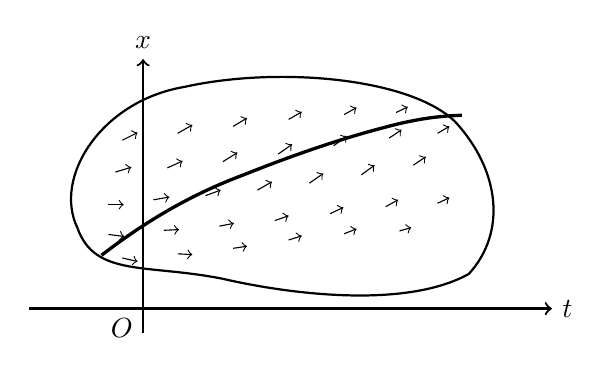
\begin{tikzpicture}[x=0.88cm,y=0.88cm,thick]
  \draw[thick] (-3.1,-0.38) .. controls (-3.45,0.35) and (-2.75,1.45) .. (-1.55,1.65)
    .. controls (-0.2,1.95) and (1.7,1.78) .. (2.35,1.15)
    .. controls (3.0,0.45) and (3.1,-0.45) .. (2.55,-1.05)
    .. controls (1.65,-1.55) and (0.0,-1.35) .. (-1.0,-1.12)
    .. controls (-2.1,-0.9) and (-2.85,-1.1) .. (-3.1,-0.38);
  \draw[->] (-3.8,-1.55)--(3.75,-1.55) node[right] {$t$};
  \draw[->] (-2.15,-1.9)--(-2.15,2.05) node[above] {$x$};
  \node[below left] at (-2.15,-1.55) {$O$};
  % A sampled direction field; each small segment has slope depending on t and x.
  \foreach \x/\y/\dx/\dy in {
  -2.65/-0.05/0.22/0.00,-2.0/0.02/0.23/0.04,-1.25/0.08/0.22/0.08,-0.5/0.16/0.21/0.12,0.25/0.26/0.20/0.14,1.0/0.38/0.19/0.14,1.75/0.52/0.18/0.12,
  -2.55/0.42/0.23/0.07,-1.8/0.48/0.22/0.10,-1.0/0.57/0.21/0.13,-0.2/0.68/0.20/0.14,0.6/0.80/0.19/0.14,1.4/0.91/0.18/0.12,2.1/0.98/0.17/0.10,
  -2.45/0.88/0.22/0.11,-1.65/0.98/0.21/0.12,-0.85/1.08/0.20/0.12,-0.05/1.18/0.19/0.11,0.75/1.25/0.18/0.10,1.5/1.28/0.17/0.08,
  -2.65/-0.48/0.23/-0.03,-1.85/-0.42/0.22/0.01,-1.05/-0.36/0.21/0.04,-0.25/-0.28/0.20/0.07,0.55/-0.18/0.19/0.09,1.35/-0.08/0.18/0.10,2.1/-0.03/0.17/0.08,
  -2.45/-0.82/0.22/-0.05,-1.65/-0.76/0.21/-0.01,-0.85/-0.68/0.20/0.03,-0.05/-0.56/0.19/0.06,0.75/-0.47/0.18/0.07,1.55/-0.43/0.17/0.05}
    {\draw[->,thin] (\x,\y)--++(\dx,\dy);}
  \draw[very thick] (-2.75,-0.78) .. controls (-2.1,-0.28) and (-1.45,0.1) .. (-0.7,0.38)
    .. controls (0.1,0.7) and (0.85,0.95) .. (1.55,1.12)
    .. controls (1.9,1.2) and (2.15,1.23) .. (2.45,1.24);
\end{tikzpicture}
}
 \caption{实心点表示取样点 \((t,y)\)，以该点为中点的短线段表示斜率 \(f(t,y)\)；粗实线为一条积分曲线，在其上的取样点处与对应短线段相切（原书图 2）。}
 \label{fig:ch1-direction-field}
\end{figure}

\paragraph{例 1：指数增长与衰减.}
为了说明定理 1，特别是它的唯一性部分的含义，求解
\begin{equation}
 y'=ay,
 \label{eq:ch1-exponential}
\end{equation}
其中 \(a\in\R\)。这里
\[
 f(t,y)=ay,\qquad \frac{\partial f}{\partial y}=a.
\]
函数实际上只依赖于 \(y\)，定义集合可以取整个平面 \(P\)。函数 \(f\) 及其偏导数在整个平面上连续，因此定理 1 适用。直接代入可知，对任意常数 \(c\in\R\)，
\begin{equation}
 y(t)=ce^{at}
 \label{eq:ch1-exponential-solutions}
\end{equation}
都是 \eqref{eq:ch1-exponential} 的解，并且都定义在整个实轴 \(-\infty<t<+\infty\) 上，所以是不可延拓解。

还要证明 \eqref{eq:ch1-exponential-solutions} 给出了全部解。设 \(y=\varphi(t)\) 是任一解，在它的定义区间中取一点 \(t_0\)，记 \(y_0=\varphi(t_0)\)。取
\[
 c=y_0e^{-at_0}.
\]
那么解 \(ce^{at}\) 与 \(\varphi(t)\) 具有相同的初始值 \((t_0,y_0)\)。由定理 1 的第二部分，它们在共同区间上相同。因此，随着 \(c\) 取遍一切实数，公式 \eqref{eq:ch1-exponential-solutions} 确实给出全部解。

\paragraph{例 2：放射性衰变.}
用 \(y(t)\) 表示到时刻 \(t\) 尚未衰变的放射性物质量。由物理上的假设，若不能追踪整个反应过程，至少可以说衰变速度与剩余物质量成正比：
\begin{equation}
 y'(t)=-\beta y(t),
 \label{eq:ch1-radioactive}
\end{equation}
其中 \(\beta>0\) 是依赖于物质性质的常数，负号表示物质量在减少。这个方程正是例 1 中 \(a=-\beta\) 的情形，所以
\[
 y(t)=ce^{-\beta t}.
\]
若已知在 \(t=0\) 时物质量为 \(y_0\)，则 \(c=y_0\)，于是
\[
 y(t)=y_0e^{-\beta t}.
\]
这里的 \(\beta\) 具有量纲 \(1/\text{秒}\)。通常用半衰期代替 \(\beta\) 描述衰变快慢。半衰期 \(T\) 是物质量减到原来一半所需的时间，因此
\[
 \frac{y_0}{2}=y_0e^{-\beta T}.
\]
当 \(y_0>0\) 时约去 \(y_0\)，得到
\[
 e^{-\beta T}=\frac12,
 \qquad
 T=\frac{\ln 2}{\beta}.
\]

\section{一些初等的求积方法}

研究微分方程时，首先遇到的通常是如何求解的问题。这与代数学中的情况类似。代数学曾试图用开根给出任意次方程的解：二次方程有求根公式，三次方程有 Cardan 公式，四次方程有 Ferrari 公式；后来证明，用根式给出四次以上方程的一般公式是不可能的。可是，始终可以求数值系数方程的近似解，也可以研究方程的根如何依赖系数。

微分方程理论早期也力图用初等函数以及这些函数的积分把解表示出来，即所谓“用求积方式积分出微分方程”。当人们弄清只有少数类型的方程才具有这种意义下的解以后，理论重点便转移到研究解的一般性质和变化规律。本节只介绍几类最简单的一阶方程，它们仍展示了“积分—隐式解—分支—唯一性”之间的关系。

\subsection{正合方程}

\textbf{(A) 正合方程.} 考虑
\begin{equation}
 y'=\frac{g(t,y)}{h(t,y)}.
 \label{eq:ch1-exact-normal}
\end{equation}
假设 \(g,h\) 在 \((t,y)\) 平面的某个开集 \(\Gamma\) 上有定义且连续；分母 \(h(t,y)\) 在 \(\Gamma\) 的每一点都不为零。再假设微分形式
\[
 h(t,y)\,\dd y-g(t,y)\,\dd t
\]
在整个 \(\Gamma\) 上是全微分。这意味着存在函数 \(F:\Gamma\to\R\)，使得
\begin{equation}
 \frac{\partial F}{\partial y}(t,y)=h(t,y),
 \qquad
 \frac{\partial F}{\partial t}(t,y)=-g(t,y).
 \label{eq:ch1-exact-potential}
\end{equation}
于是 \eqref{eq:ch1-exact-normal} 可以约定地写成
\[
 h(t,y)\,\dd y-g(t,y)\,\dd t=0,
\]
而左边正是 \(\dd F\)。

\begin{proposition}[正合方程的解]
 \label{prop:ch1-exact}
 在以上条件下，方程 \eqref{eq:ch1-exact-normal} 的每一个解 \(y=\varphi(t)\) 都满足
 \[
  F(t,\varphi(t))=\text{常数}.
 \]
 反之，由含任意常数 \(c\) 的隐式关系
 \begin{equation}
  F(t,y)=c
  \label{eq:ch1-exact-integral}
 \end{equation}
 在某个区间上确定的可微函数 \(y=\varphi(t)\)，都是方程 \eqref{eq:ch1-exact-normal} 的解。
\end{proposition}

\begin{proof}
先设 \(y=\varphi(t)\) 是 \eqref{eq:ch1-exact-normal} 在区间 \(r_1<t<r_2\) 上的解。对这个区间中的每个 \(t\)，都有
\[
 h(t,\varphi(t))\varphi'(t)-g(t,\varphi(t))=0.
\]
由 \eqref{eq:ch1-exact-potential}，左边正是 \(F(t,\varphi(t))\) 对 \(t\) 的全导数：
\[
 \frac{\dd}{\dd t}F(t,\varphi(t))
 =F_t(t,\varphi(t))+F_y(t,\varphi(t))\varphi'(t)
 =-g(t,\varphi(t))+h(t,\varphi(t))\varphi'(t)=0.
\]
根据微积分中的已知结论，在连通区间上导数为零的函数为常数，所以 \(F(t,\varphi(t))\) 在整个定义区间上为常数。

反过来，若 \(y=\varphi(t)\) 是由 \eqref{eq:ch1-exact-integral} 定义的解，即 \(F(t,\varphi(t))\equiv c\)，对 \(t\) 求导，得到
\[
 F_t(t,\varphi(t))+F_y(t,\varphi(t))\varphi'(t)=0.
\]
代入 \eqref{eq:ch1-exact-potential}，便有
\[
 h(t,\varphi(t))\varphi'(t)-g(t,\varphi(t))=0.
\]
因为 \(h\neq0\)，这正是 \eqref{eq:ch1-exact-normal}。命题得证。
\end{proof}

几何上，方程 \eqref{eq:ch1-exact-normal} 的每一条积分曲线都完全位于函数 \(F(t,y)\) 的某条水平线
\[
 F(t,y)=c
\]
上。反过来，每一条水平线的连通部分，只要能够表示为某个区间上的函数 \(y=\varphi(t)\)，就是积分曲线。可是，水平线可能由分开的几段组成；在这种情况下，一个常数 \(c\) 可能确定几条不同的积分曲线。换言之，同一个隐式公式可能对应几个，甚至无限多个，不可延拓解。例 3 将具体展示这一点。

\subsection{一阶线性方程}

\textbf{(B) 线性方程.} 求解
\begin{equation}
 y'=a(t)y+b(t),
 \label{eq:ch1-linear-scalar}
\end{equation}
其中 \(a(t),b(t)\) 在区间
\[
 I=(r_1,r_2)
\]
上有定义且连续，端点可以取无穷。此时
\[
 \Gamma=I\times\R.
\]
若两个端点都有限，则 \(\Gamma\) 是带形区域；若只有一个端点有限，则它是半平面；若两个端点为无穷，则 \(\Gamma\) 是整个平面。在整个 \(\Gamma\) 上，方程右端及其对 \(y\) 的偏导数都连续，所以定理 1 的条件满足。

固定 \(t_0\in I\)，记
\begin{equation}
 A(t)=\int_{t_0}^{t}a(s)\,\dd s.
 \label{eq:ch1-linear-integrated-coefficient}
\end{equation}
函数 \(A(t)\) 在整个 \(I\) 上有定义。方程 \eqref{eq:ch1-linear-scalar} 的全部解可写成
\begin{equation}
 y(t)=e^{A(t)}
 \left(
  c+\int_{t_0}^{t}e^{-A(s)}b(s)\,\dd s
 \right),
 \qquad c\in\R.
 \label{eq:ch1-linear-solution}
\end{equation}
这些解都在整个 \(I\) 上有定义，因而是相对于给定定义域 \(I\times\R\) 的不可延拓解：在区间端点之外，方程右端本来就没有定义。

\begin{proof}[公式 \eqref{eq:ch1-linear-solution} 的验证与完整性]
先验证这些函数确实是解。由微积分基本定理，
\[
 \frac{\dd}{\dd t}e^{A(t)}=a(t)e^{A(t)},
 \qquad
 \frac{\dd}{\dd t}\int_{t_0}^{t}e^{-A(s)}b(s)\,\dd s
 =e^{-A(t)}b(t).
\]
因此
\[
 \begin{aligned}
  y'(t)
  &=a(t)e^{A(t)}
    \left(c+\int_{t_0}^{t}e^{-A(s)}b(s)\,\dd s\right)
    +e^{A(t)}e^{-A(t)}b(t)\\
  &=a(t)y(t)+b(t).
 \end{aligned}
\]

现在证明公式包含全部解。设 \(y=\varphi(t)\) 是 \eqref{eq:ch1-linear-scalar} 在某个区间 \(J\subseteq I\) 上的任意解，取 \(\tau_0\in J\)，令 \(\xi_0=\varphi(\tau_0)\)。需要选择常数 \(c\)，使公式给出的解在 \(\tau_0\) 处等于 \(\xi_0\)。条件为
\[
 \left(
  c+\int_{t_0}^{\tau_0}e^{-A(s)}b(s)\,\dd s
 \right)e^{A(\tau_0)}
 =\xi_0.
\]
这是关于 \(c\) 的一次方程，而且未知量 \(c\) 的系数 \(e^{A(\tau_0)}\) 不为零，所以可唯一地解出
\[
 c=\xi_0e^{-A(\tau_0)}
 -\int_{t_0}^{\tau_0}e^{-A(s)}b(s)\,\dd s.
\]
由定理 1 的唯一性，公式给出的解与 \(\varphi\) 在共同定义区间上完全相同。因此公式 \eqref{eq:ch1-linear-solution} 包含全部解。
\end{proof}

为了与教科书中常见的记忆方法对照，可以重新推导这个公式。先考虑齐次方程
\begin{equation}
 y'=a(t)y.
 \label{eq:ch1-linear-homogeneous}
\end{equation}
在 \(y\neq0\) 时，把它写成
\[
 \frac{\dd y}{y}-a(t)\,\dd t=0.
\]
这是正合方程。取
\[
 F(t,y)=\ln|y|-A(t),
\]
则齐次解由
\[
 \ln|y|-A(t)=c_1
\]
确定，即
\begin{equation}
 y=ce^{A(t)}.
 \label{eq:ch1-linear-homogeneous-solution}
\end{equation}
这里 \(c\) 可以取任意实数；\(y=0\) 对应 \(c=0\)。严格地说，先除以 \(y\) 的推导没有覆盖 \(y=0\)，但这个遗漏可以由公式的完整性证明，或由 \(c=0\) 补上，因此不影响齐次解公式。

再用常数变易法求非齐次解。设
\[
 y=c(t)e^{A(t)},
\]
其中 \(c(t)\) 是待定函数。代入 \eqref{eq:ch1-linear-scalar}，得到
\[
 c'(t)e^{A(t)}+c(t)a(t)e^{A(t)}
 =a(t)c(t)e^{A(t)}+b(t).
\]
含有 \(a(t)\) 的项相消，于是
\[
 c'(t)e^{A(t)}=b(t),
 \qquad
 c(t)=c_0+\int_{t_0}^{t}e^{-A(s)}b(s)\,\dd s.
\]
代回即得 \eqref{eq:ch1-linear-solution}。这就是常数变易法：把齐次解中的常数换成时间函数。

\subsection{例题}

\paragraph{例 1：可分离变量方程.}
求解
\begin{equation}
 y'=f(t)g(y).
 \label{eq:ch1-separable}
\end{equation}
假设 \(f(t)\) 在区间 \(r_1<t<r_2\) 上有定义且连续；\(g(y)\) 在区间 \(q_1<y<q_2\) 上有定义、连续且处处不为零。于是方程可以约定写成
\[
 \frac{\dd y}{g(y)}-f(t)\,\dd t=0.
\]
取
\[
 F(t,y)=\int_{y_0}^{y}\frac{\dd \xi}{g(\xi)}
 -\int_{t_0}^{t}f(\tau)\,\dd \tau,
\]
其中 \(y_0\) 属于区间 \((q_1,q_2)\)，\(t_0\) 属于区间 \((r_1,r_2)\)。根据正合方程命题，全部解由隐式关系
\begin{equation}
 \int_{y_0}^{y(t)}\frac{\dd \xi}{g(\xi)}
 =
 \int_{t_0}^{t}f(\tau)\,\dd \tau+c
 \label{eq:ch1-separable-integral}
\end{equation}
确定。

条件 \(g\neq0\) 是分离变量时除法的要求。若原方程在某个零点 \(g(y_*)=0\) 附近有定义，应当把常数解 \(y\equiv y_*\) 单独检查，不能因为公式中出现了除法就把这些解删去。

\paragraph{例 2：右端只依赖于比值的所谓齐次方程.}
求解
\begin{equation}
 y'=h\left(\frac{y}{t}\right).
 \label{eq:ch1-ratio-equation}
\end{equation}
这里“齐次”是指右端只依赖于比值 \(y/t\)，与线性方程中“自由项为零”的齐次含义不同。假设 \(h(u)\) 在某个区间上有定义且连续，并且在该区间上
\[
 h(u)-u\neq0.
\]
在不含 \(t=0\) 的区间上引入新未知函数
\[
 u(t)=\frac{y(t)}{t},
 \qquad y=tu.
\]
求导得 \(y'=u+tu'\)，因此原方程化为
\[
 u+tu'=h(u),
 \qquad
 u'=\frac{h(u)-u}{t}.
\]
这就是可分离变量方程：
\[
 \frac{\dd u}{h(u)-u}=\frac{\dd t}{t}.
\]
按例 1 求出 \(u\)，再由 \(y=tu\) 返回原未知函数。

若某个 \(u_*\) 满足 \(h(u_*)=u_*\)，则直接检查可知 \(y=u_*t\) 是直线解。原书在 \(h(u)-u\neq0\) 的区域上用分离变量讨论，正是为了避免除零。

\paragraph{例 3：一个公式可能给出无限多个最大解.}
求解
\begin{equation}
 y'=y^2\cos t.
 \label{eq:ch1-branch-example}
\end{equation}
它的定义集合是整个 \((t,y)\) 平面。当 \(y>0\) 或 \(y<0\) 时，可以用可分离变量法：
\[
 \int\frac{\dd y}{y^2}=\int\cos t\,\dd t.
\]
于是
\[
 -\frac1y=\sin t-c,
\]
即
\begin{equation}
 y(t)=\frac{1}{c-\sin t}.
 \label{eq:ch1-branch-formula}
\end{equation}
除这个公式表示的解以外，还有显然的解
\begin{equation}
 y(t)\equiv0.
 \label{eq:ch1-zero-solution}
\end{equation}

公式 \eqref{eq:ch1-branch-formula} 与零解已经包括方程的全部解。设 \((t_0,y_0)\) 为任意初始值。若 \(y_0=0\)，零解满足这个初始条件。若 \(y_0\neq0\)，取
\[
 c=\sin t_0+\frac1{y_0},
\]
则公式 \eqref{eq:ch1-branch-formula} 给出的解在 \(t_0\) 处取值 \(y_0\)。由唯一性，不再有其他解。

接下来必须按定义区间分类。零解定义在整个实轴上，因而不可延拓。当
\[
 |c|>1
\]
时，分母 \(c-\sin t\) 始终不为零，公式在整条实轴上定义，构成一个不可延拓解。当
\[
 |c|<1
\]
时，方程 \(\sin t=c\) 有无穷多个解，相邻两个零点为 \(r_1<r_2\)。在每一个区间
\[
 r_1<t<r_2
\]
上，公式给出一个单独的不可延拓解；到了端点，分母趋于零，解不能继续作为有限实值解延拓。当 \(|c|=1\) 时，端点情形相同，也要按相邻零点之间分段理解。

因此，只要 \(|c|\le1\)，同一个常数 \(c\) 和同一个代数公式 \eqref{eq:ch1-branch-formula} 就给出无限多个解，而不是一个解。图~\ref{fig:ch1-branches} 上方画出辅助曲线 \(y=c-\sin t\) 的零点，下方画出对应的倒数分支。

\begin{figure}[H]
 \centering
 \resizebox{0.72\textwidth}{!}{\begin{tikzpicture}[x=0.48cm,y=0.43cm,thick]
  % Upper graph: y=c-sin(t), with c=1/2 and two adjacent roots marked.
  \draw[->] (-5.9,0)--(13.9,0) node[right] {$t$};
  \draw[->] (0,-1.5)--(0,1.75) node[above] {$y$};
  \draw[domain=-5.8:13.8,samples=220,smooth,variable=\t] plot (\t,{0.5-sin(57.2958*\t)});
  \fill (0.524,0) circle (1.4pt) node[below] {$r_1$};
  \fill (2.618,0) circle (1.4pt) node[below] {$r_2$};
  \node at (9.6,-1.05) {$y=c-\sin t$};
  % Reciprocal branches; vertical dashed lines are singular times.
  \begin{scope}[yshift=-5.0cm]
    \draw[->] (-5.9,0)--(13.9,0) node[right] {$t$};
    \draw[->] (0,-3.1)--(0,3.1) node[above] {$y$};
    \foreach \a in {-5.76,0.524,6.807,13.091} {\draw[dashed,thin] (\a,-3.05)--(\a,3.05);}
    \foreach \a in {-3.665,2.618,8.901} {\draw[dashed,thin] (\a,-3.05)--(\a,3.05);}
    \draw[domain=-5.70:-3.72,samples=100,smooth,variable=\t] plot (\t,{max(-3,min(3,1/(0.5-sin(57.2958*\t))))});
    \draw[domain=-3.60:0.45,samples=120,smooth,variable=\t] plot (\t,{max(-3,min(3,1/(0.5-sin(57.2958*\t))))});
    \draw[domain=0.60:2.55,samples=100,smooth,variable=\t] plot (\t,{max(-3,min(3,1/(0.5-sin(57.2958*\t))))});
    \draw[domain=2.70:6.75,samples=120,smooth,variable=\t] plot (\t,{max(-3,min(3,1/(0.5-sin(57.2958*\t))))});
    \draw[domain=6.90:8.85,samples=100,smooth,variable=\t] plot (\t,{max(-3,min(3,1/(0.5-sin(57.2958*\t))))});
    \draw[domain=8.97:13.0,samples=120,smooth,variable=\t] plot (\t,{max(-3,min(3,1/(0.5-sin(57.2958*\t))))});
    \node at (10.9,-4.20) {$y=\dfrac{1}{c-\sin t}$};
    \fill (0.524,0) circle (1.4pt) node[below] {$r_1$};
    \fill (2.618,0) circle (1.4pt) node[below] {$r_2$};
  \end{scope}
\end{tikzpicture}
}
 \caption{辅助曲线的零点决定倒数公式的各个最大解分支（原书图 3）。}
 \label{fig:ch1-branches}
\end{figure}

\paragraph{例 4：右端连续仍可能失去唯一性.}
考虑
\begin{equation}
 y'=3y^{2/3},
 \qquad
 y^{2/3}=(\sqrt[3]{y})^2.
 \label{eq:ch1-nonunique}
\end{equation}
右端对所有 \(y\in\R\) 都有定义且连续；但它的导函数
\[
 \frac{\partial}{\partial y}\bigl(3y^{2/3}\bigr)=2y^{-1/3}
\]
在 \(y=0\) 处不存在，并在那里出现间断。如果把整个平面作为定义域，定理 1 的条件不满足。若只在
\[
 y>0\quad\text{或}\quad y<0
\]
的半平面中讨论，定理 1 仍可应用，分离变量得到
\[
 y^{1/3}=t-c,
\]
或者
\begin{equation}
 y=(t-c)^3.
 \label{eq:ch1-cubic-solutions}
 \end{equation}
当 \(t<c\) 时，这个函数的一部分位于半平面 \(y<0\)；当 \(t>c\) 时，另一部分位于半平面 \(y>0\)。

可是，直接代入可知，公式 \eqref{eq:ch1-cubic-solutions} 在整个实轴上都满足方程 \eqref{eq:ch1-nonunique}；同时 \(y\equiv0\) 也是解。于是，通过直线 \(y=0\) 上的每一点 \((t,y)=(c,0)\)，至少存在两个解：三次函数 \eqref{eq:ch1-cubic-solutions} 和零解。图~\ref{fig:ch1-nonunique} 给出若干条三次曲线，它们都在 \(y=0\) 上与零解相切。

这个例子说明：只有右端连续而不具备连续的状态偏导数时，唯一性结论可能失败。它没有断言“偏导数不连续必然失去唯一性”；定理 1 的条件是保证唯一性的充分条件。

\begin{figure}[H]
 \centering
 \resizebox{0.62\textwidth}{!}{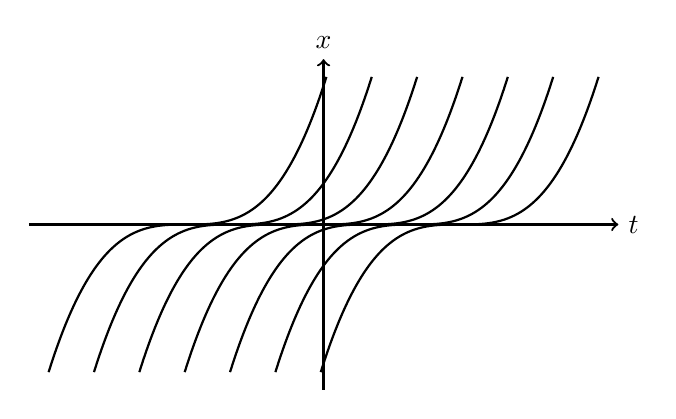
\begin{tikzpicture}[x=0.72cm,y=0.75cm,thick]
  \draw[->] (-5.2,0)--(5.2,0) node[right] {$t$};
  \draw[->] (0,-2.8)--(0,2.8) node[above] {$x$};
  \foreach \c in {-2.4,-1.6,-0.8,0,0.8,1.6,2.4} {
    \pgfmathsetmacro{\lo}{\c-2.45}
    \pgfmathsetmacro{\hi}{\c+2.45}
    \draw[domain=\lo:\hi,samples=90,smooth,variable=\t]
      plot (\t,{0.17*(\t-\c)^3});
  }
\end{tikzpicture}
}
 \caption{连续但不满足状态偏导数条件的右端使得同一初始值可对应多个解（原书图 4）。}
 \label{fig:ch1-nonunique}
\end{figure}

\section{存在和唯一性定理的叙述}

§1 讨论了一个一阶微分方程，并叙述了它的存在和唯一性定理。常微分方程理论还要处理更一般的方程组。通常，由几个一阶方程组成的系统含有几个未知函数，而这些未知函数都是同一个自变量的函数。无论方程的形式如何，存在和唯一性定理都是研究给定微分方程组的理论基础。

原书先对一种表面形式较特殊的系统叙述并证明定理；实际上，相当一般的系统都可以化成这种形式。这种特殊形式称为标准方程组。用现代列向量记号，标准系统就是
\begin{equation}
 \vect{x}'=\vect{f}(t,\vect{x}),
 \qquad
 \vect{f}:\Omega\subseteq\R\times\R^n\to\R^n.
 \label{eq:ch1-standard-system}
\end{equation}
分量形式为
\begin{equation}
 x_i'=f_i(t,x_1,\ldots,x_n),
 \qquad i=1,\ldots,n.
 \label{eq:ch1-standard-components}
\end{equation}
这里 \(t\) 是自变量，\(x_1,\ldots,x_n\) 是未知函数，而 \(f_1,\ldots,f_n\) 定义在 \(n+1\) 维空间中的开集 \(\Omega\) 上。\(\Omega\) 中点的坐标是
\[
 (t,x_1,\ldots,x_n).
\]
今后总假设 \(\vect{f}\) 在 \(\Omega\) 上连续，并且它的状态偏导数
\begin{equation}
 \frac{\partial f_i}{\partial x_j}(t,\vect{x}),
 \qquad i,j=1,\ldots,n,
 \label{eq:ch1-state-partials}
\end{equation}
在 \(\Omega\) 上存在且连续。这里强调：这些偏导数只关于 \(x_1,\ldots,x_n\) 求，不要求关于 \(t\) 的偏导数存在。

连续向量函数 \(\vect{x}:I\to\R^n\) 是系统 \eqref{eq:ch1-standard-system} 的解，是指它在 \(I\) 上可微，并且在每个 \(t\in I\) 处都有
\[
 (t,\vect{x}(t))\in\Omega,
 \qquad
 \vect{x}'(t)=\vect{f}(t,\vect{x}(t)).
\]
区间 \(I\) 称为解的定义区间，不排除 \(I=(-\infty,+\infty)\) 的情形。“在区间上满足方程组”是指把 \(x_1(t),\ldots,x_n(t)\) 代入后得到整个区间上的恒等式；因此既要求 \(\vect{x}(t)\) 在每一点可微，也要求代换后的点始终落在右端函数的定义域中。

\begin{theorem}[标准方程组的存在唯一性]
 \label{thm:ch1-system-existence}
 设 \eqref{eq:ch1-standard-system} 是标准方程组，\(\vect{f}\) 在开集 \(\Omega\subseteq\R\times\R^n\) 上有定义且连续，并且 \(D_{\vect{x}}\vect{f}\) 在 \(\Omega\) 上存在且连续。则：
 \begin{enumerate}[label=\arabic*.]
  \item 对 \(\Omega\) 中每一点 \((t_0,\vect{x}_0)\)，存在一个包含 \(t_0\) 的区间上的解 \(\vect{x}=\vect{\varphi}(t)\)，满足
  \[
   \vect{\varphi}(t_0)=\vect{x}_0.
  \]
  \item 若两个解 \(\vect{x}=\vect{\psi}(t)\) 和 \(\vect{x}=\vect{\chi}(t)\) 的定义区间都含有 \(t_0\)，并且
  \[
   \vect{\psi}(t_0)=\vect{\chi}(t_0),
  \]
  则它们在共同定义区间上处处相等。
 \end{enumerate}
\end{theorem}

证明见\hyperref[sec:existence-proofs]{本章补证}。补证在开集 \(\Omega\)、\(\vect{f}\) 连续且 \(D_{\vect{x}}\vect{f}\) 连续的条件下，用向量形式的 Picard 逐次逼近构造局部解；随后沿公共区间反复使用局部唯一性，得到整个公共区间上的唯一性；最大解一节再把所有同初值解合并成唯一的不可延拓解。

向量
\[
 \vect{x}_0=
 \begin{pmatrix}
  x_{10}\\
  \vdots\\
  x_{n0}
 \end{pmatrix}
\]
称为初始值，关系式
\begin{equation}
 \vect{x}(t_0)=\vect{x}_0
 \label{eq:ch1-initial-condition}
\end{equation}
称为初始条件。说一个解具有初始值 \(\vect{x}_0\)，总表示它的定义区间含有 \(t_0\)。定理 2 可以简述为：对任意初始值，总存在以它为初值的局部解；若两个解具有相同初值，则它们在共同定义区间上完全重合。

完全与 §1 一样，可以定义延拓和不可延拓解。设 \(\vect{x}:I\to\R^n\) 和 \(\vect{\widetilde{x}}:J\to\R^n\) 都是同一系统的解，且 \(I\subseteq J\)，\(\vect{\widetilde{x}}|_I=\vect{x}\)，则称 \(\vect{\widetilde{x}}\) 是 \(\vect{x}\) 的延拓。特别地，自身也算自身的一个延拓。若不存在任何不同于它自身、却仍以它为限制的延拓，则称该解不可延拓。在定理 2 的条件下，每一个解都可以唯一地延拓到不可延拓解；详细证明见\hyperref[sec:existence-proofs]{本章补证}中的“最大解的存在与唯一”一节。

\begin{theorem}[线性系统的整体存在性]
 \label{thm:ch1-linear-existence}
 设
 \begin{equation}
  \vect{x}'=\mat{A}(t)\vect{x}+\vect{b}(t)
  \label{eq:ch1-linear-system}
 \end{equation}
 是标准线性系统，其中
 \[
  \mat{A}:I\to\R^{n\times n},
  \qquad
  \vect{b}:I\to\R^n
 \]
 在区间 \(I=(q_1,q_2)\) 上连续。则对任意 \(t_0\in I\) 和任意 \(\vect{x}_0\in\R^n\)，系统 \eqref{eq:ch1-linear-system} 存在一个以
 \[
  \vect{x}(t_0)=\vect{x}_0
 \]
 为初始条件、并且在整个区间 \(I\) 上有定义的解。
 \end{theorem}

特别地，如果 \(\mat{A}(t)\) 和 \(\vect{b}(t)\) 在整条实轴上连续，即 \(q_1=-\infty,q_2=+\infty\)，那么对任意初值，系统都存在定义在整个无限区间 \(-\infty<t<+\infty\) 上的解。结合定理 2，整个区间上的解还是唯一的。这个结论将在\hyperref[sec:existence-proofs]{本章补证}的“线性系统为何在系数连续的整个区间上存在”一节中证明；线性迭代差的阶乘估计使逐次逼近在每个紧子区间上收敛，而不需要把时间区间缩小到压缩系数小于一。

标准系统的解有直接的几何意义。以
\[
 t,x_1,\ldots,x_n
\]
为坐标得到 \(n+1\) 维空间；解 \(\vect{x}=\vect{\varphi}(t)\) 对应于曲线
\begin{equation}
 t\longmapsto
 \begin{pmatrix}
  t\\
  \varphi_1(t)\\
  \vdots\\
  \varphi_n(t)
 \end{pmatrix}
 \in\R^{n+1}.
 \label{eq:ch1-integral-curve-system}
\end{equation}
这条曲线称为系统的积分曲线。它的切向量为
\[
 \begin{pmatrix}
  1\\
  x_1'(t)\\
  \vdots\\
  x_n'(t)
 \end{pmatrix}
 =
 \begin{pmatrix}
  1\\
  f_1(t,\vect{x}(t))\\
  \vdots\\
  f_n(t,\vect{x}(t))
 \end{pmatrix}.
\]
系统本身在 \(\Omega\) 的每一点规定了方向 \((1,\vect{f}(t,\vect{x}))\)，于是得到 \(n+1\) 维空间中的方向场。这个方向场是 §1 平面情形的高维类比。

\subsection{例题}

\paragraph{例 1：平面旋转系统.}
求解
\begin{equation}
 x_1'=-\omega x_2,
 \qquad
 x_2'=\omega x_1,
 \label{eq:ch1-rotation}
\end{equation}
其中 \(\omega\) 是实常数。集合 \(\Omega\) 是坐标 \((t,x_1,x_2)\) 的整个三维空间。直接求导可知
\begin{equation}
 x_1(t)=c_1\cos(\omega t+c_2),
 \qquad
 x_2(t)=c_1\sin(\omega t+c_2)
 \label{eq:ch1-rotation-solution}
\end{equation}
是解，其中 \(c_1,c_2\) 是常数。

要证明 \eqref{eq:ch1-rotation-solution} 包含全部解，只需证明任意初值都能由适当的常数实现。给定初值 \((t_0,x_{10},x_{20})\)，令 \((\rho,\varphi)\) 是点 \((x_{10},x_{20})\) 的极坐标，因此
\[
 x_{10}=\rho\cos\varphi,
 \qquad
 x_{20}=\rho\sin\varphi.
\]
把初值代入 \eqref{eq:ch1-rotation-solution}，得到决定 \(c_1,c_2\) 的条件
\[
 c_1\cos(\omega t_0+c_2)=x_{10},
 \qquad
 c_1\sin(\omega t_0+c_2)=x_{20}.
\]
利用极坐标化为
\[
 c_1\cos(\omega t_0+c_2)=\rho\cos\varphi,
 \qquad
 c_1\sin(\omega t_0+c_2)=\rho\sin\varphi.
\]
取
\[
 c_1=\rho,
 \qquad
 c_2=\varphi-\omega t_0,
\]
这两式便同时成立。若 \((x_{10},x_{20})=\vect{0}\)，取 \(\rho=0\) 即可。因此通过每一点 \((t_0,x_{10},x_{20})\) 都有公式 \eqref{eq:ch1-rotation-solution} 给出的解；由定理 2 的唯一性，公式包含全部解。

用矩阵写成
\[
 \vect{x}'=
 \begin{pmatrix}
  0&-\omega\\
  \omega&0
 \end{pmatrix}\vect{x},
\]
可以更直接看出右端是线性的。后文将利用复指数函数再次求解这类系统。

\paragraph{例 2：右端的光滑性与解的光滑性.}
证明：如果标准系统 \eqref{eq:ch1-standard-system} 的右端 \(\vect{f}\) 是 \(k\) 次连续可微的，也就是说 \(\vect{f}\) 对全部变量 \(t,x_1,\ldots,x_n\) 具有直到 \(k\) 阶的连续偏导数，并且包括混合偏导数，那么它的任一解 \(\vect{x}=\vect{\varphi}(t)\) 具有 \(k+1\) 阶连续导数。

事实上，对于解有恒等式
\begin{equation}
 \varphi_i'(t)=f_i(t,\varphi_1(t),\ldots,\varphi_n(t)),
 \qquad i=1,\ldots,n.
 \label{eq:ch1-solution-identity}
\end{equation}
如果 \(\vect{f}\) 具有连续的一阶偏导数，那么恒等式右端对 \(t\) 有连续导数，因此 \(\varphi_i'(t)\) 连续可微，从而 \(\varphi_i''(t)\) 存在且连续。对恒等式 \eqref{eq:ch1-solution-identity} 逐次求导，并反复使用链式法则，就可以依次证明
\[
 \varphi_i',\varphi_i'',\ldots,\varphi_i^{(k+1)}
\]
的存在性和连续性。用矩阵写出一阶导数的显式公式就是
\[
 \vect{x}''(t)
 =\vect{f}_t(t,\vect{x}(t))+D_{\vect{x}}\vect{f}(t,\vect{x}(t))\vect{x}'(t).
\]
继续求导时，还会出现 \(\vect{f}\) 的各高阶状态偏导数和混合偏导数，这正是题设要求它们连续的原因。

\section{化一般微分方程组为标准方程组}

前一节对标准方程组叙述了解的存在和唯一性定理。现在说明怎样把相当一般的高阶微分方程组化为标准方程组；同时，一般方程组的存在和唯一性结论也由此得到。

先给出一般微分方程的形式。一个未知函数 \(y\) 的方程可以写为
\begin{equation}
 F(t,y,y',\ldots,y^{(n)})=0,
 \label{eq:ch1-general-high-order}
\end{equation}
其中 \(t\) 是自变量，\(y\) 是未知函数，\(F\) 是给定的 \(n+2\) 个变量的函数。函数 \(F\) 未必对所有变量值都有定义，所以需要谈它的定义域 \(B\)，其中 \(B\) 是坐标
\[
 t,y,y',\ldots,y^{(n)}
\]
的 \(n+2\) 维空间中的开集。如果方程中导数的最高阶数等于 \(n\)，就称它是 \(n\) 阶方程。

如果定义在区间 \(r_1<t<r_2\) 上的函数 \(y=\varphi(t)\) 具有直到 \(n\) 阶的导数，使得
\[
 \bigl(t,\varphi(t),\varphi'(t),\ldots,\varphi^{(n)}(t)\bigr)\in B
\]
在整个区间上成立，并且代入后使 \eqref{eq:ch1-general-high-order} 成为恒等式，则称它是该方程的解。与一阶情形一样，必须同时检查所需导数的存在性和右端定义域。

若有同一自变量的两个未知函数 \(u,v\)，则两个微分方程组成的方程组可以写成
\begin{equation}
 \begin{cases}
  F(t,u,u',\ldots,u^{(m)},v,v',\ldots,v^{(n)})=0,\\
  G(t,u,u',\ldots,u^{(m)},v,v',\ldots,v^{(n)})=0.
 \end{cases}
 \label{eq:ch1-two-unknown-general}
\end{equation}
其中 \(F,G\) 定义在某个开集 \(B\) 上。若 \(u\) 在方程中出现的最高导数阶数为 \(m\)，\(v\) 的最高导数阶数为 \(n\)，则分别称 \(m,n\) 为方程组关于 \(u,v\) 的阶，并称
\[
 m+n
\]
为整个方程组的阶。定义在共同区间上的一对函数 \(u=\varphi(t),v=\psi(t)\) 若代入后使两个方程在整个区间上恒成立，就称为方程组的解。

对未知函数 \(y_1,\ldots,y_r\) 同样可以定义方程组。若 \(y_i\) 在方程组中出现的最高导数阶数为 \(q_i\)，则
\[
 q=q_1+\cdots+q_r
\]
称为方程组的阶。§3 的标准方程组按这种计数法是一阶方程组，因为它只含一阶导数，并且有 \(n\) 个未知函数，所以总阶数为 \(n\)。

如果关系式 \eqref{eq:ch1-general-high-order} 可以关于 \(y^{(n)}\) 解出，就得到
\begin{equation}
 y^{(n)}=f(t,y,y',\ldots,y^{(n-1)}).
 \label{eq:ch1-explicit-high-order}
\end{equation}
同样，如果两个未知函数的方程组可以关于 \(u^{(m)},v^{(n)}\) 解出，就得到
\begin{equation}
 \begin{cases}
  u^{(m)}
  =f(t,u,u',\ldots,u^{(m-1)},v,v',\ldots,v^{(n-1)}),\\
  v^{(n)}
  =g(t,u,u',\ldots,u^{(m-1)},v,v',\ldots,v^{(n-1)}).
 \end{cases}
 \label{eq:ch1-explicit-two-high-order}
\end{equation}
这两类方程称为已解出最高阶导数的方程。任意多个未知函数的方程也可以类似定义。今后几乎只研究已解出最高阶导数的系统；§3 的标准一阶系统正是其中的特殊情形。

现在证明：任何已解出最高阶导数的 \(n\) 阶微分方程组，都可以化为标准一阶方程组。先处理一个 \(n\) 阶标量方程。

\subsection{一个高阶方程的转化}

\textbf{(A) 一个 \(n\) 阶方程.} 设
\begin{equation}
 y^{(n)}=f(t,y,y',\ldots,y^{(n-1)})
 \label{eq:ch1-high-order-scalar}
\end{equation}
是一个已解出最高阶导数的 \(n\) 阶微分方程。这里 \(t\) 是自变量，\(y\) 是未知函数。函数 \(f\) 定义在 \(n+1\) 维坐标空间中的开集 \(\Gamma\) 内，其坐标是
\[
 t,y,y',\ldots,y^{(n-1)}.
\]
假设 \(f\) 在 \(\Gamma\) 上连续，并且它关于各个状态变量
\[
 y,y',\ldots,y^{(n-1)}
\]
的偏导数在 \(\Gamma\) 上也连续。这里把 \(y,y',\ldots,y^{(n-1)}\) 看成彼此独立的坐标。

为了把 \eqref{eq:ch1-high-order-scalar} 化为标准系统，引入新未知函数
\begin{equation}
 x_1=y,\qquad x_2=y',\qquad \ldots,\qquad x_n=y^{(n-1)}.
 \label{eq:ch1-companion-coordinates}
\end{equation}
把它们排成状态列向量
\begin{equation}
 \vect{x}(t)=
 \begin{pmatrix}
  x_1(t)\\
  x_2(t)\\
  \vdots\\
  x_n(t)
 \end{pmatrix}
 =
 \begin{pmatrix}
  y(t)\\
  y'(t)\\
  \vdots\\
  y^{(n-1)}(t)
 \end{pmatrix}
 \in\R^n.
 \label{eq:ch1-scalar-state}
\end{equation}
方程 \eqref{eq:ch1-high-order-scalar} 等价于标准系统
\begin{equation}
 \begin{cases}
  x_1'=x_2,\\
  x_2'=x_3,\\
  \qquad\vdots\\
  x_{n-1}'=x_n,\\
  x_n'=f(t,x_1,x_2,\ldots,x_n).
 \end{cases}
 \label{eq:ch1-companion-system}
\end{equation}
用向量形式写作
\begin{equation}
 \vect{x}'=
 \begin{pmatrix}
  x_2\\
  x_3\\
  \vdots\\
  x_n\\
  f(t,x_1,\ldots,x_n)
 \end{pmatrix}.
 \label{eq:ch1-companion-vector}
\end{equation}

下面证明“等价”在两个方向上成立。先设 \(y=\varphi(t)\) 满足 \eqref{eq:ch1-high-order-scalar}。由 \eqref{eq:ch1-companion-coordinates} 定义
\[
 x_1=\varphi,\quad x_2=\varphi',\quad\ldots,\quad x_n=\varphi^{(n-1)}.
\]
对关系式求导，得到
\begin{equation}
 x_k'=y^{(k)}=x_{k+1},
 \qquad k=1,\ldots,n-1,
 \label{eq:ch1-companion-first-equations}
\end{equation}
而
\begin{equation}
 x_n'=y^{(n)}
 =f(t,y,y',\ldots,y^{(n-1)})
 =f(t,x_1,x_2,\ldots,x_n).
 \label{eq:ch1-companion-last-equation}
\end{equation}
所以 \(\vect{x}\) 满足系统 \eqref{eq:ch1-companion-system}。

反过来，设 \(\vect{x}=(x_1,\ldots,x_n)\) 满足系统 \eqref{eq:ch1-companion-system}，并令 \(y=x_1\)。系统第一式给出
\[
 y'=x_1'=x_2.
\]
第二式给出
\[
 y''=x_2'=x_3.
\]
继续逐式代换，得到
\[
 y^{(k)}=x_{k+1},
 \qquad k=0,\ldots,n-1.
\]
最后，在系统最后一式中代入这些关系：
\[
 y^{(n)}=x_n'
 =f(t,x_1,\ldots,x_n)
 =f(t,y,y',\ldots,y^{(n-1)}).
\]
所以 \(y\) 满足原高阶方程。两段构造互相逆转，故在共同区间上，原方程的解与系统 \eqref{eq:ch1-companion-system} 的解一一对应。

原方程的初始条件通常写成
\begin{equation}
 y^{(k)}(t_0)=y_{0}^{(k)},
 \qquad k=0,1,\ldots,n-1.
 \label{eq:ch1-high-order-initial}
\end{equation}
它在变换 \eqref{eq:ch1-companion-coordinates} 下恰好变成状态初值
\begin{equation}
 \vect{x}(t_0)=
 \begin{pmatrix}
  y_0\\
  y_0'\\
  \vdots\\
  y_0^{(n-1)}
 \end{pmatrix}.
 \label{eq:ch1-state-initial}
\end{equation}
要求
\[
 (t_0,y_0,y_0',\ldots,y_0^{(n-1)})\in\Gamma.
\]
由于 \eqref{eq:ch1-companion-vector} 的右端及其 Jacobian 在相应开集上连续，定理 2 给出满足这些初始条件的局部解，并断言两个具有相同状态初值的解在共同区间上相同。

如果原方程是线性的，即
\begin{equation}
 y^{(n)}
 =a_0(t)y+a_1(t)y'+\cdots+a_{n-1}(t)y^{(n-1)}+q(t),
 \label{eq:ch1-linear-high-order}
\end{equation}
并且系数 \(a_0,\ldots,a_{n-1}\) 与自由项 \(q\) 在区间 \(I=(q_1,q_2)\) 上连续，那么系统 \eqref{eq:ch1-companion-system} 也是线性的：
\begin{equation}
 \vect{x}'=\mat{A}(t)\vect{x}+\vect{b}(t),
 \label{eq:ch1-high-order-linear-system}
\end{equation}
其中
\begin{equation}
 \mat{A}(t)=
 \begin{pmatrix}
  0&1&0&\cdots&0\\
  0&0&1&\cdots&0\\
  \vdots&\vdots&\vdots&\ddots&\vdots\\
  0&0&0&\cdots&1\\
  a_0(t)&a_1(t)&a_2(t)&\cdots&a_{n-1}(t)
 \end{pmatrix},
 \qquad
 \vect{b}(t)=
 \begin{pmatrix}
  0\\
  0\\
  \vdots\\
  0\\
  q(t)
 \end{pmatrix}.
 \label{eq:ch1-companion-linear-data}
\end{equation}
由定理 3，任意初始条件 \eqref{eq:ch1-high-order-initial} 都确定一个在整个 \(I\) 上定义的解。这就是命题 (A) 的最后一项整体存在结论。

\subsection{多个高阶方程的转化}

\textbf{(B) 两个二阶方程组成的方程组.} 为减少记号上的复杂性，原书以两个二阶方程为例：
\begin{equation}
 \begin{cases}
  u''=f(t,u,u',v,v'),\\
  v''=g(t,u,u',v,v').
 \end{cases}
 \label{eq:ch1-two-second-order}
\end{equation}
按照
\begin{equation}
 x_1=u,\qquad x_2=u',\qquad x_3=v,\qquad x_4=v'
 \label{eq:ch1-two-state-coordinates}
\end{equation}
引入新的未知函数后，方程组化成
\begin{equation}
 \begin{cases}
  x_1'=x_2,\\
  x_2'=f(t,x_1,x_2,x_3,x_4),\\
  x_3'=x_4,\\
  x_4'=g(t,x_1,x_2,x_3,x_4).
 \end{cases}
 \label{eq:ch1-two-standard-system}
\end{equation}
用列向量写就是
\begin{equation}
 \vect{x}'=
 \begin{pmatrix}
  x_2\\
  f(t,x_1,x_2,x_3,x_4)\\
  x_4\\
  g(t,x_1,x_2,x_3,x_4)
 \end{pmatrix}.
 \label{eq:ch1-two-standard-vector}
\end{equation}

假设右端函数 \(f,g\) 在五维空间中坐标为
\[
 t,u,u',v,v'
\]
的某个开集 \(\Gamma\) 上有定义且连续，并且它们关于四个状态变量的偏导数也连续，那么在 \eqref{eq:ch1-two-standard-vector} 经过坐标变换后，新的右端满足定理 2 的条件。于是对 \(\Gamma\) 中任一点
\[
 (t_0,u_0,p_0,v_0,q_0),
\]
存在满足
\begin{equation}
 u(t_0)=u_0,\qquad u'(t_0)=p_0,
 \qquad
 v(t_0)=v_0,\qquad v'(t_0)=q_0
 \label{eq:ch1-two-initial-conditions}
\end{equation}
的解 \(u=\varphi(t),v=\psi(t)\)。此外，任何两个具有同样初始条件的解，在它们定义区间的公共部分上相同。

命题 (B) 的证明与命题 (A) 完全一样。正向地，对方程组 \eqref{eq:ch1-two-second-order} 的解按 \eqref{eq:ch1-two-state-coordinates} 定义 \(x_1,\ldots,x_4\)，求导便得到系统 \eqref{eq:ch1-two-standard-system}。反向地，若 \(x_1,\ldots,x_4\) 满足该系统，令 \(u=x_1,v=x_3\)，第一式和第三式给出
\[
 u'=x_2,
 \qquad
 v'=x_4,
\]
第二式和第四式再给出原来的两个二阶方程。初始条件也在变换 \eqref{eq:ch1-two-state-coordinates} 下逐项对应。因此原方程组的解与四维标准系统的解一一对应。

对更多未知函数，做法完全相同：依次把每个未知函数和它低于最高阶的各阶导数排入状态向量。若各未知函数的最高阶数分别为 \(q_1,\ldots,q_r\)，则状态向量有
\[
 q_1+\cdots+q_r
\]
个分量。这样就把总阶数有限的已解出最高阶导数系统化成了标准一阶系统。

\subsection{尚未解出最高阶导数时的问题}

如果 \(n\) 阶方程仍以
\begin{equation}
 F(t,y,y',\ldots,y^{(n)})=0
 \label{eq:ch1-implicit-high-order}
\end{equation}
给出，而没有解出未知函数的最高阶导数 \(y^{(n)}\)，那么首先出现的问题是：能否在给定区域中解出 \(y^{(n)}\)。这更像一个函数论中的隐函数问题，但它会把一些新的现象带入微分方程研究。

例如，若 \(F\) 关于 \(y^{(n)}\) 是二次的，那么在其他变量固定时，方程可能确定 \(y^{(n)}\) 的两个值。如果这两个值在某一区域内处处不同，就可以分别研究两个形如
\[
 y^{(n)}=f_\pm(t,y,y',\ldots,y^{(n-1)})
\]
的已解出方程。但如果两个值在某个集合上重合，或不能连续地分成彼此分离的分支，就不能简单地把原方程拆成两个标准方程。研究这种情形会导致微分方程奇解的概念，以及与曲面上微分方程有关的理论。原书不讨论这些问题；本节的转化结论始终以最高阶导数已经显式解出为前提。

\subsection{例题}

\paragraph{例 1：简谐振动方程.}
求解
\begin{equation}
 y''+\omega^2y=0,
 \qquad \omega>0.
 \label{eq:ch1-harmonic}
\end{equation}
直接验证可知，函数
\begin{equation}
 y(t)=r\cos(\omega t+\alpha),
 \qquad r\ge0,
 \label{eq:ch1-harmonic-solution}
\end{equation}
满足这个方程，其中 \(r,\alpha\) 是常数。

还要证明公式 \eqref{eq:ch1-harmonic-solution} 包含全部解。设 \(y=\varphi(t)\) 是任一解。由线性高阶方程的整体存在结论，也就是命题 (A) 的末尾部分，可以认为这个解对所有 \(t\in\R\) 有定义。令
\[
 y(0)=y_0,
 \qquad
 y'(0)=v_0.
\]
直接验证可以选取常数 \(r,\alpha\)，使
\begin{equation}
 r\cos\alpha=y_0,
 \qquad
 -r\omega\sin\alpha=v_0.
 \label{eq:ch1-harmonic-initial-match}
\end{equation}
如果这些等式成立，那么公式 \eqref{eq:ch1-harmonic-solution} 给出的解与原解有相同的初始值 \((0,y_0,v_0)\)，由命题 (A) 和唯一性，它们相同。

为具体选出 \(r,\alpha\)，当 \((y_0,v_0)\neq(0,0)\) 时取
\[
 r=\sqrt{y_0^2+\frac{v_0^2}{\omega^2}},
\]
并要求
\[
 \cos\alpha=\frac{y_0}{r},
 \qquad
 \sin\alpha=-\frac{v_0}{\omega r}.
\]
两式的平方和为
\[
 \frac{y_0^2}{r^2}+\frac{v_0^2}{\omega^2r^2}=1,
\]
所以这样的 \(\alpha\) 存在；若 \(y_0=v_0=0\)，取 \(r=0\) 即可。因此公式 \eqref{eq:ch1-harmonic-solution} 确实给出全部解。

函数 \eqref{eq:ch1-harmonic-solution} 描述简谐振动。正数 \(r\) 称为振幅，\(\alpha\) 称为初相位，简称相位。方程 \eqref{eq:ch1-harmonic} 称为简谐振动方程。数 \(\omega\) 称为角频率；每单位时间内完成完整振动的次数为
\begin{equation}
 \nu=\frac{\omega}{2\pi}.
 \label{eq:ch1-frequency-harmonic}
\end{equation}
用状态 \(\vect{x}=(y,y')\) 表示，方程是
\[
 \vect{x}'=
 \begin{pmatrix}
  0&1\\
  -\omega^2&0
 \end{pmatrix}\vect{x}.
\]
两个状态分量分别是位移与速度；初值 \(\vect{x}(0)=(y_0,v_0)\) 正好同时给出这两个信息。

\paragraph{例 2：弹性回复力下的直线运动.}
讨论质量为 \(m\) 的质点 \(p\) 在力 \(F\) 的作用下沿水平直线 \(L\) 的运动。设力始终沿该直线指向固定点 \(O\)，大小与 \(p\) 到 \(O\) 的距离成正比。在直线上取 \(O\) 为原点，用 \(x=x(t)\) 表示质点 \(p\) 的有符号坐标。在物理记号中，对时间的一阶、二阶导数写为 \(\dot x,\ddot x\)。根据牛顿第二定律，
\begin{equation}
 m\ddot x=F=-kx,
 \qquad k>0.
 \label{eq:ch1-spring-newton}
\end{equation}
通常写成
\begin{equation}
 m\ddot x+kx=0.
 \label{eq:ch1-spring}
\end{equation}
负号自动处理原点两侧：当 \(x>0\) 时，力指向负方向；当 \(x<0\) 时，力指向正方向。

在物理上，这种回复力可以由弹簧实现，如图~\ref{fig:ch1-spring} 所示。数 \(k\) 称为弹簧的弹性系数。把 \eqref{eq:ch1-spring} 除以 \(m\)，与例 1 比较，得到
\begin{equation}
 x(t)=r\cos\left(\sqrt{\frac{k}{m}}\,t+\alpha\right),
 \qquad r\ge0.
 \label{eq:ch1-spring-solution}
\end{equation}
于是质点 \(p\) 的角频率
\[
 \omega=\sqrt{\frac{k}{m}}
\]
由质量 \(m\) 和弹性系数 \(k\) 决定，与初始条件无关。振幅 \(r\) 和初相位 \(\alpha\) 则与初始条件有关，也就是与 \(t=0\) 时质点 \(p\) 的位置 \(x(0)\) 和速度 \(\dot x(0)\) 有关。

\begin{figure}[H]
 \centering
 \resizebox{0.78\textwidth}{!}{\begin{tikzpicture}[x=0.8cm,y=0.8cm,thick]
  % Fixed supports and a mass between two elastic springs.
  \fill[pattern=north east lines] (-4.1,-0.58) rectangle (-3.85,0.58);
  \fill[pattern=north east lines] (3.85,-0.58) rectangle (4.1,0.58);
  \draw[thick] (-3.85,0)--(3.85,0);
  \draw[decorate,decoration={coil,aspect=0.5,segment length=4mm,amplitude=3mm}] (-3.65,0)--(-0.65,0);
  \draw[decorate,decoration={coil,aspect=0.5,segment length=4mm,amplitude=3mm}] (0.65,0)--(3.65,0);
  \draw[fill=white,thick] (0,0) circle (0.48);
  \fill (0,0) circle (1.6pt);
  \node at (0.72,0.58) {$p$};
  \draw[<->] (-0.05,0.88)--(1.45,0.88) node[midway,above] {$x$};
  \draw[->] (0,-0.72)--(-1.55,-0.72) node[midway,below] {$F$};
\end{tikzpicture}
}
 \caption{弹性回复力下的直线运动；位移 \(x\) 和回复力 \(F\) 取有符号方向（原书图 5）。}
 \label{fig:ch1-spring}
\end{figure}

\paragraph{例 3：数学摆的小振动.}
数学摆由一个质量为 \(m\) 的质点 \(p\) 组成；在重力作用下，质点沿竖直平面内半径为 \(\ell\) 的圆周 \(K\) 运动，\(\ell\) 称为摆长。取圆周最低点 \(O\) 为角坐标零点，在圆周上取正方向，用 \(\theta=\theta(t)\) 表示质点的变动角坐标，如图~\ref{fig:ch1-pendulum} 所示。为与全文三角函数记号一致，这里把原书的 \(\varphi\) 写为 \(\theta\)。

作用在质点 \(p\) 上的重力大小为 \(mg\)，方向竖直向下。重力沿圆周法线方向的分量由约束力提供的方向相反作用来平衡；重力的切向分量，若取角增加的方向为正，则等于
\[
 -mg\sin\theta.
\]
沿切线应用牛顿第二定律，质点的加速度为 \(\ell\ddot\theta\)，于是
\[
 m\ell\ddot\theta=-mg\sin\theta,
\]
或者
\begin{equation}
 \ell\ddot\theta+g\sin\theta=0.
 \label{eq:ch1-pendulum}
\end{equation}
这个方程是非线性的，求它的精确解相当困难。若在运动中角 \(\theta\) 始终与零相差很小，就可以用 \(\theta\) 代替 \(\sin\theta\)，得到摆的近似方程
\begin{equation}
 \ell\ddot\theta+g\theta=0.
 \label{eq:ch1-pendulum-linearized}
\end{equation}
它的解具有例 1 的形式：
\begin{equation}
 \theta(t)=r\cos\left(\sqrt{\frac{g}{\ell}}\,t+\alpha\right).
 \label{eq:ch1-pendulum-small-solution}
\end{equation}
因此摆的小振动角频率为
\[
 \omega=\sqrt{\frac{g}{\ell}},
\]
单位时间内完整振动次数为
\[
 \nu=\frac{\omega}{2\pi}
 =\frac{1}{2\pi}\sqrt{\frac{g}{\ell}}.
\]
例如秒摆，即每秒振动一次的摆，满足 \(\nu=1\,\mathrm{s}^{-1}\)。于是
\[
 \ell=\frac{g}{4\pi^2}\approx 0.25\,\mathrm m.
\]
这里的余弦解是小角近似方程的解，而不是非线性摆方程 \eqref{eq:ch1-pendulum} 的精确解。精确摆方程可写成标准状态系统
\[
 x_1=\theta,\quad x_2=\dot\theta,
 \qquad
 \begin{cases}
  x_1'=x_2,\\
  x_2'=-\dfrac{g}{\ell}\sin x_1.
 \end{cases}
\]

\begin{figure}[H]
 \centering
 \resizebox{0.58\textwidth}{!}{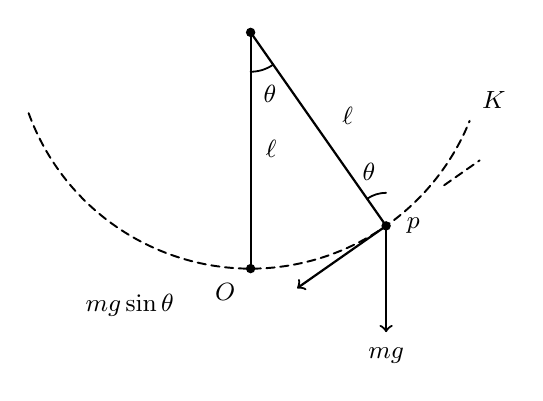
\begin{tikzpicture}[
  x=1cm,
  y=1cm,
  line cap=round,
  line join=round,
  every node/.style={font=\small}
]
  % 以悬点为圆心，O 和 p 同在半径为 l 的圆弧上。
  \def\radius{3}
  \def\swingangle{35}
  \pgfmathsetmacro{\px}{\radius*sin(\swingangle)}
  \pgfmathsetmacro{\py}{\radius-\radius*cos(\swingangle)}
  \pgfmathsetmacro{\topEndAngle}{270+\swingangle}
  \pgfmathsetmacro{\pEndAngle}{90+\swingangle}
  \pgfmathsetmacro{\pLabelAngle}{90+\swingangle/2}

  \coordinate (C) at (0,\radius);
  \coordinate (O) at (0,0);
  \coordinate (P) at (\px,\py);
  \coordinate (Kleft) at ({\radius*cos(200)},{\radius+\radius*sin(200)});
  \coordinate (Kright) at ({\radius*cos(338)},{\radius+\radius*sin(338)});
  \coordinate (TopAngleStart) at ({0.50*cos(270)},{\radius+0.50*sin(270)});
  \coordinate (TopAngleLabel) at ({0.82*cos(270+\swingangle/2)},{\radius+0.82*sin(270+\swingangle/2)});
  \coordinate (PAngleStart) at ({\px+0.42*cos(90)},{\py+0.42*sin(90)});
  \coordinate (PAngleLabel) at ({\px+0.72*cos(\pLabelAngle)},{\py+0.72*sin(\pLabelAngle)});

  % 轨道圆弧，以原图的悬点为圆心。
  \draw[densely dashed, line width=0.7pt]
    (Kleft) arc[start angle=200,end angle=338,radius=\radius cm];

  % 悬点到最低点和质点的两条半径。
  \draw[line width=0.8pt] (C)--(O);
  \draw[line width=0.8pt] (C)--(P)
    node[pos=0.56,above right=2pt] {$\ell$};
  \node[right=2pt] at (0,1.52) {$\ell$};

  % p 点处的切线及重力、切向分量。
  \pgfmathsetmacro{\tangentStartX}{\px+0.90*cos(\swingangle)}
  \pgfmathsetmacro{\tangentStartY}{\py+0.90*sin(\swingangle)}
  \pgfmathsetmacro{\tangentEndX}{\px+1.45*cos(\swingangle)}
  \pgfmathsetmacro{\tangentEndY}{\py+1.45*sin(\swingangle)}
  \pgfmathsetmacro{\componentEndX}{\px-1.38*cos(\swingangle)}
  \pgfmathsetmacro{\componentEndY}{\py-1.38*sin(\swingangle)}
  \draw[densely dashed, line width=0.7pt]
    (\tangentStartX,\tangentStartY)--(\tangentEndX,\tangentEndY);
  \draw[->,line width=0.8pt] (P)--(\px,\py-1.35)
    node[below=2pt] {$mg$};
  \draw[->,line width=0.8pt] (P)--(\componentEndX,\componentEndY);
  \node[anchor=east] at (-0.85,-0.46) {$mg\sin\theta$};

  % 两处角标相同：摆杆与竖直方向的夹角。
  \draw[line width=0.65pt] (TopAngleStart)
    arc[start angle=270,end angle=\topEndAngle,radius=0.50cm];
  \node at (TopAngleLabel) {$\theta$};
  \draw[line width=0.65pt] (PAngleStart)
    arc[start angle=90,end angle=\pEndAngle,radius=0.42cm];
  \node at (PAngleLabel) {$\theta$};

  \fill (C) circle (1.7pt);
  \fill (O) circle (1.7pt);
  \fill (P) circle (1.7pt);
  \node[below left=2pt] at (O) {$O$};
  \node[right=4pt] at (P) {$p$};
  \node[above right=1pt] at (Kright) {$K$};
\end{tikzpicture}
}
 \caption{数学摆的角坐标 $\theta$ 与重力的切向分量（据原书图 6 重绘）。}
 \label{fig:ch1-pendulum}
\end{figure}

\section{复值微分方程}

直到现在，只讨论了实值微分方程及其实解。但在某些情况下，例如求解常系数线性方程时，先求出实方程的复值解，再由复值解取得实解会更方便。为了说明这个过程，必须引入实变量的复值函数，以及复值微分方程组。

\subsection{实变量的复值函数}

\textbf{(A) 复值函数.} 如果对区间 \(r_1<t<r_2\) 上的每一个实数值 \(t\)，有复数
\begin{equation}
 z(t)=u(t)+iv(t)
 \label{eq:ch1-complex-function}
\end{equation}
与之对应，其中 \(u(t),v(t)\) 是实变量的实函数，则称 \(z\) 是实变量 \(t\) 的复值函数。函数 \(u\) 称为 \(z\) 的实部，\(v\) 称为 \(z\) 的虚部：
\[
 u(t)=\operatorname{Re}z(t),
 \qquad
 v(t)=\operatorname{Im}z(t).
\]
如果 \(u,v\) 连续，就称复值函数 \(z\) 连续；如果 \(u,v\) 可微，就称 \(z\) 可微，并定义
\begin{equation}
 z'(t)=u'(t)+iv'(t).
 \label{eq:ch1-complex-derivative}
\end{equation}
这里 \(t\) 仍然是实变量，所以这是沿实轴求导，而不是复分析意义下的全纯导数。

直接验证可知，实变量的复值函数仍满足通常的和、积、商求导法则；商法则要求分母不为零。例如
\[
 (z_1z_2)'
 =z_1'z_2+z_1z_2'.
\]
复向量值函数的连续性、可微性按每个分量定义。

\subsection{复系统的实化}

\textbf{(B) 标准复方程组.} 考虑
\begin{equation}
 \vect{z}'=\vect{h}(t,\vect{z}),
 \qquad
 \vect{z}(t)\in\C^n,
 \qquad
 \vect{h}:\Omega\subseteq\R\times\C^n\longrightarrow\C^n.
 \label{eq:ch1-complex-system}
\end{equation}
为了避免复分析中额外的可微性理论，本章按原书范围假设 \(\vect{h}\) 的每个分量都是复变量 \(z_1,\ldots,z_n\) 的多项式，并且多项式系数是实变量 \(t\) 在区间 \(I=(q_1,q_2)\) 上的连续实值或复值函数。在这个条件下，\(\vect{h}\) 对任意 \(\vect{z}\in\C^n\) 都有定义。

若定义在某个区间上的复值向量函数 \(\vect{z}(t)\) 代入 \eqref{eq:ch1-complex-system} 后得到恒等式，就称它是解。对任意 \(t_0\in I\) 和任意 \(\vect{z}_0\in\C^n\)，系统存在满足
\begin{equation}
 \vect{z}(t_0)=\vect{z}_0
 \label{eq:ch1-complex-initial}
\end{equation}
的局部解；具有相同初值的两个解在共同定义区间上相同。若系统是线性的，则解在整个 \(I\) 上有定义。

这些结论可以直接由定理 2 推出。把每个复未知函数分成实部和虚部：
\begin{equation}
 z_j=x_j+iy_j,
 \qquad j=1,\ldots,n.
 \label{eq:ch1-complex-real-components}
\end{equation}
在 \eqref{eq:ch1-complex-system} 中用 \(x_j+iy_j\) 代替 \(z_j\)，得到
\begin{equation}
 \dot x_j+i\dot y_j
 =f_j(t,x_1,\ldots,x_n,y_1,\ldots,y_n)
 +ig_j(t,x_1,\ldots,x_n,y_1,\ldots,y_n),
 \label{eq:ch1-complex-realified-component}
\end{equation}
其中 \(f_j,g_j\) 都是实变量的实值函数，并满足
\begin{equation}
 f_j+ig_j
 =h_j(t,x_1+iy_1,\ldots,x_n+iy_n).
 \label{eq:ch1-complex-real-part-definition}
\end{equation}
比较 \eqref{eq:ch1-complex-realified-component} 两边的实部和虚部，就得到实系统
\begin{equation}
 \begin{cases}
  x_j'=f_j(t,x_1,\ldots,x_n,y_1,\ldots,y_n),\\
  y_j'=g_j(t,x_1,\ldots,x_n,y_1,\ldots,y_n),
 \end{cases}
 \qquad j=1,\ldots,n.
 \label{eq:ch1-complex-realified-system}
\end{equation}
因为 \(\vect{h}\) 关于复变量是多项式，所以 \(f_j,g_j\) 关于 \(2n\) 个实变量 \(x_1,\ldots,x_n,y_1,\ldots,y_n\) 也是多项式；又因为 \(\vect{h}\) 的系数关于 \(t\) 连续，所以 \(f_j,g_j\) 的系数也关于 \(t\) 连续。于是实系统 \eqref{eq:ch1-complex-realified-system} 满足定理 2 的条件。

若
\[
 \vect{z}_0=\vect{x}_0+i\vect{y}_0,
\]
则复初始条件 \eqref{eq:ch1-complex-initial} 等价于实初始条件
\begin{equation}
 \vect{x}(t_0)=\vect{x}_0,
 \qquad
 \vect{y}(t_0)=\vect{y}_0.
 \label{eq:ch1-complex-real-initial}
\end{equation}
定理 2 给出实系统的局部存在唯一性；反过来，任何一个实系统解都可以通过 \(\vect{z}=\vect{x}+i\vect{y}\) 组成复系统解。因为两个复数相等当且仅当实部、虚部分别相等，所以这个对应在两个方向上都成立。

对线性复系统，实化可以写得很明确。设
\begin{equation}
 \vect{z}'=\mat{A}(t)\vect{z}+\vect{b}(t),
 \qquad
 \mat{A}(t)=\mat{B}(t)+i\mat{C}(t),
 \quad
 \vect{b}(t)=\vect{p}(t)+i\vect{q}(t),
 \label{eq:ch1-complex-linear}
\end{equation}
其中 \(\mat{B}(t),\mat{C}(t)\in\R^{n\times n}\)，\(\vect{p}(t),\vect{q}(t)\in\R^n\)。若 \(\vect{z}=\vect{x}+i\vect{y}\)，则
\[
 (\mat{B}+i\mat{C})(\vect{x}+i\vect{y})
 =(\mat{B}\vect{x}-\mat{C}\vect{y})+i(\mat{C}\vect{x}+\mat{B}\vect{y}).
\]
因此 \eqref{eq:ch1-complex-linear} 等价于
\begin{equation}
 \frac{\dd}{\dd t}
 \begin{pmatrix}
  \vect{x}\\\vect{y}
 \end{pmatrix}
 =
 \begin{pmatrix}
  \mat{B}(t)&-\mat{C}(t)\\
  \mat{C}(t)&\mat{B}(t)
 \end{pmatrix}
 \begin{pmatrix}
  \vect{x}\\\vect{y}
 \end{pmatrix}
 +
 \begin{pmatrix}
  \vect{p}(t)\\\vect{q}(t)
 \end{pmatrix}.
 \label{eq:ch1-complex-linear-realified}
\end{equation}
这是 \(2n\) 维实线性系统，系数连续，因此由定理 3，解在整个 \(I\) 上存在。矩阵 \eqref{eq:ch1-complex-linear-realified} 中的四个块顺序不能随意调换：左上、右下分别来自 \(\mat{A}\) 的实部和虚部，右上块带负号，左下块带正号。

最后指出，右端为复变量多项式的复系统，其多项式系数可能全部是 \(t\) 的实函数。即使如此，仍可把 \(z_1,\ldots,z_n\) 看成复变量并寻找复值解。这样做是因为某些实系统求复值解比直接求实值解更容易。先求复值解，再从中分出实值解；所谓分出，就是只保留虚部恒为零的那些复值解。对一般非线性方程，不能把任意复值解的实部直接当作实值解。

\subsection{高阶复方程}

\textbf{(C) \(n\) 阶复方程.} 设
\begin{equation}
 z^{(n)}
 =f(t,z,z',\ldots,z^{(n-1)})
 \label{eq:ch1-complex-high-order}
\end{equation}
是 \(n\) 阶复值方程。假设右端是关于复变量
\[
 z,z',\ldots,z^{(n-1)}
\]
的多项式，其系数是实变量 \(t\) 在 \(I=(q_1,q_2)\) 上的实值或复值连续函数。如果
\[
 t_0\in I,
\]
而 \(z_0,z_0',\ldots,z_0^{(n-1)}\) 是任意复数，那么方程 \eqref{eq:ch1-complex-high-order} 存在满足
\begin{equation}
 z(t_0)=z_0,
 \quad
 z'(t_0)=z_0',
 \quad
 \ldots,
 \quad
 z^{(n-1)}(t_0)=z_0^{(n-1)}
 \label{eq:ch1-complex-high-order-initial}
\end{equation}
的局部复值解。任何两个具有相同初始条件的解，在定义区间的公共部分上相同。若方程是线性的，即右端多项式关于各状态变量是一次多项式，则对任意初始值，解都在整个 \(I\) 上有定义。

证明与 §4 命题 (A) 相同。令
\begin{equation}
 \vect{\zeta}=
 \begin{pmatrix}
  z\\z'\\\vdots\\z^{(n-1)}
 \end{pmatrix}
 \in\C^n.
 \label{eq:ch1-complex-state}
\end{equation}
原方程等价于复标准系统
\begin{equation}
 \vect{\zeta}'=
 \begin{pmatrix}
  \zeta_2\\
  \zeta_3\\
  \vdots\\
  \zeta_n\\
  f(t,\zeta_1,\ldots,\zeta_n)
 \end{pmatrix}.
 \label{eq:ch1-complex-companion}
\end{equation}
正向地，若 \(z\) 满足高阶方程，按 \eqref{eq:ch1-complex-state} 定义状态向量，逐分量求导即得系统。反向地，令 \(z=\zeta_1\)；系统前 \(n-1\) 式依次给出
\[
 \zeta_{k+1}=z^{(k)},
 \ k=0,\ldots,n-1,
\]
最后一式给出原高阶方程。新的右端是复变量的多项式，因此前面复系统实化的存在唯一性结论适用；线性高阶方程产生线性复系统，整体存在性由定理 3 的复值版本得到。

\subsection{复指数函数}

\textbf{(D) \(e^w\) 的定义与性质.} 令 \(w=u+iv\) 是任意复数，定义
\begin{equation}
 e^w=e^u(\cos v+i\sin v).
 \label{eq:ch1-complex-exponential-definition}
\end{equation}
由此容易看出
\begin{equation}
 e^{\overline w}=\overline{e^w}.
 \label{eq:ch1-complex-conjugate-exponential}
\end{equation}
下面证明乘法公式
\begin{equation}
 e^{w_1}e^{w_2}=e^{w_1+w_2}.
 \label{eq:ch1-complex-exponential-product}
\end{equation}
由此可直接取得 Euler 公式：
\begin{equation}
 \cos v=\frac{e^{iv}+e^{-iv}}2,
 \qquad
 \sin v=\frac{e^{iv}-e^{-iv}}{2i}.
 \label{eq:ch1-euler-formulas}
\end{equation}
若 \(\lambda=\mu+i\nu\) 是复数，则根据定义
\begin{equation}
 e^{\lambda t}
 =e^{\mu t}
 \bigl(\cos(\nu t)+i\sin(\nu t)\bigr).
 \label{eq:ch1-exponential-real-time}
\end{equation}

也可以用幂级数
\begin{equation}
 e^w=1+w+\frac{w^2}{2!}+\frac{w^3}{3!}+\cdots
 \label{eq:ch1-complex-exponential-series}
\end{equation}
定义 \(e^w\)，再证明它与 \eqref{eq:ch1-complex-exponential-definition} 相同。原书把三角函数定义式 \eqref{eq:ch1-complex-exponential-definition} 作为出发点，本稿沿用这一安排。

现在证明乘法公式。设
\[
 w_1=u_1+iv_1,
 \qquad
 w_2=u_2+iv_2.
\]
由定义和三角函数和角公式，
\[
 \begin{aligned}
 e^{w_1}e^{w_2}
 &=e^{u_1}(\cos v_1+i\sin v_1)
   e^{u_2}(\cos v_2+i\sin v_2)\\
 &=e^{u_1+u_2}
   \bigl(\cos(v_1+v_2)+i\sin(v_1+v_2)\bigr)\\
 &=e^{w_1+w_2}.
 \end{aligned}
\]
特别地，由 \(e^{iv}e^{-iv}=1\) 和上述乘法公式即可得到 \eqref{eq:ch1-euler-formulas}。

再证明关于实时间 \(t\) 的求导公式
\begin{equation}
 \frac{\dd}{\dd t}e^{\lambda t}
 =\lambda e^{\lambda t}.
 \label{eq:ch1-complex-exponential-derivative}
\end{equation}
先讨论纯虚数 \(\lambda=iv\) 的情形：
\[
 \begin{aligned}
 \frac{\dd}{\dd t}e^{ivt}
 &=\frac{\dd}{\dd t}\bigl(\cos vt+i\sin vt\bigr)\\
 &=-v\sin vt+iv\cos vt\\
 &=iv(\cos vt+i\sin vt)
 =iv e^{ivt}.
 \end{aligned}
\]
对于任意 \(\lambda=\mu+i\nu\)，由
\[
 e^{\lambda t}=e^{\mu t}e^{i\nu t}
\]
和乘积求导法则，得到
\[
 \begin{aligned}
 \frac{\dd}{\dd t}e^{\lambda t}
 &=
 \left(\frac{\dd}{\dd t}e^{\mu t}\right)e^{i\nu t}
 +e^{\mu t}\frac{\dd}{\dd t}e^{i\nu t}\\
 &=\mu e^{\mu t}e^{i\nu t}
 +i\nu e^{\mu t}e^{i\nu t}
 =(\mu+i\nu)e^{\lambda t}
 =\lambda e^{\lambda t}.
 \end{aligned}
\]

\subsection{复值方程例题}

\paragraph{例 1：复指数解与二维实系统.}
讨论复方程
\begin{equation}
 z'=\lambda z,
 \qquad
 z=x+iy,
 \qquad
 \lambda=\mu+i\nu,
 \label{eq:ch1-complex-linear-example}
\end{equation}
其中 \(z\) 是实变量 \(t\) 的复值未知函数。由公式 \eqref{eq:ch1-complex-exponential-derivative}，对任意复常数 \(c\)，
\begin{equation}
 z(t)=ce^{\lambda t}
 \label{eq:ch1-complex-exponential-solution}
\end{equation}
都是 \eqref{eq:ch1-complex-linear-example} 的解。

要证明 \eqref{eq:ch1-complex-exponential-solution} 包含全部解，可以像 §1 例 1 那样使用唯一性；这里改用定理 3，以便稍微简化计算。由于方程是线性复方程，可以认为任一解对所有实数值 \(t\) 都有定义。设任一解为 \(z=\chi(t)\)，令 \(z(0)=z_0\)。在 \eqref{eq:ch1-complex-exponential-solution} 中取 \(c=z_0\)，得到
\[
 z=z_0e^{\lambda t},
\]
它与 \(\chi(t)\) 具有相同的初始值 \((0,z_0)\)。由唯一性，两者相同。因此全部解都由 \eqref{eq:ch1-complex-exponential-solution} 给出。

若 \(c=re^{i\alpha}\)，其中 \(r>0\)、\(\alpha\in\R\)，则非零解可以写成
\begin{equation}
 z(t)=re^{\lambda t+i\alpha}.
 \label{eq:ch1-complex-polar-solution}
\end{equation}
若 \(c=0\)，取 \(r=0\) 即可。把 \eqref{eq:ch1-complex-linear-example} 分成实部和虚部：
\[
 x'+iy'=(\mu+i\nu)(x+iy)
 =(\mu x-\nu y)+i(\nu x+\mu y).
\]
于是
\begin{equation}
 \begin{cases}
  x'=\mu x-\nu y,\\
  y'=\nu x+\mu y.
 \end{cases}
 \label{eq:ch1-complex-real-system-example}
\end{equation}
两个实方程的方程组 \eqref{eq:ch1-complex-real-system-example} 等价于一个复方程 \eqref{eq:ch1-complex-linear-example}。再把 \eqref{eq:ch1-complex-polar-solution} 展开：
\[
 \begin{aligned}
 x(t)+iy(t)
 &=re^{\mu t}
 \bigl(\cos(\nu t+\alpha)+i\sin(\nu t+\alpha)\bigr),
 \end{aligned}
\]
因此
\begin{equation}
 \begin{cases}
  x(t)=re^{\mu t}\cos(\nu t+\alpha),\\
  y(t)=re^{\mu t}\sin(\nu t+\alpha).
 \end{cases}
 \label{eq:ch1-complex-real-solution-example}
\end{equation}
用复数乘法求出的实系统解 \eqref{eq:ch1-complex-real-solution-example}，正是复方法的价值所在。写成矩阵就是
\[
 \frac{\dd}{\dd t}
 \begin{pmatrix}
  x\\y
 \end{pmatrix}
 =
 \begin{pmatrix}
  \mu&-\nu\\
  \nu&\mu
 \end{pmatrix}
 \begin{pmatrix}
  x\\y
 \end{pmatrix}.
\]

\paragraph{例 2：非线性复方程的实化.}
设
\begin{equation}
 z'=z^2+iz,
 \qquad
 z=x+iy,
 \label{eq:ch1-nonlinear-complex-example}
\end{equation}
其中 \(z\) 是实变量 \(t\) 的复值未知函数。把右端展开：
\[
 (x+iy)^2+i(x+iy)
 =x^2-y^2+2ixy+ix-y
 =x^2-y^2-y+i(2xy+x).
\]
比较实部和虚部，原复方程等价于
\begin{equation}
 \begin{cases}
  x'=x^2-y^2-y,\\
  y'=2xy+x.
 \end{cases}
 \label{eq:ch1-nonlinear-complex-real-system}
\end{equation}
这个例子说明，即使不求解，也可以通过实化把一个复方程化为两个实方程。

\section{线性微分方程的基本性质}

如果在微分方程组中出现的所有未知函数以及它们的导数都是一次的，那么就称这个方程组是线性的。因此，线性微分方程组的一般形式可以写成
\begin{equation}
 \sum_{j,k}a_{ijk}(t)(x_j)^{(k)}+b_i(t)=0,
 \qquad i=1,\ldots,n.
 \label{eq:ch1-linear-general-components}
\end{equation}
这里 \(x_1,\ldots,x_n\) 是自变量 \(t\) 的未知函数，系数 \(a_{ijk}(t)\) 和自由项 \(b_i(t)\) 都是 \(t\) 的函数。若所有自由项恒等于零，就称方程组为齐次的。从每一个线性方程组中丢掉自由项，就得到与它对应的齐次方程组：
\begin{equation}
 \sum_{j,k}a_{ijk}(t)(x_j)^{(k)}=0,
 \qquad i=1,\ldots,n.
 \label{eq:ch1-linear-homogeneous-components}
\end{equation}

下面的性质都假设所有系数和自由项在共同区间
\[
 I=(q_1,q_2)
\]
上有定义且连续，所讨论的解都在整个 \(I\) 上给定。为了用矩阵书写，令出现的最高导数阶数为 \(N\)，并把没有出现的项系数补为零。定义
\begin{equation}
 \mat{A}_k(t)=\bigl(a_{ijk}(t)\bigr)_{i,j=1}^{n},
 \qquad
 k=0,\ldots,N,
 \label{eq:ch1-linear-coefficient-matrices}
\end{equation}
以及
\begin{equation}
 \vect{b}(t)=
 \begin{pmatrix}
  b_1(t)\\
  \vdots\\
  b_n(t)
 \end{pmatrix},
 \qquad
 \vect{x}^{(0)}(t)=\vect{x}(t).
 \label{eq:ch1-linear-forcing-vector}
\end{equation}
那么 \eqref{eq:ch1-linear-general-components} 可以写成
\begin{equation}
 \sum_{k=0}^{N}\mat{A}_k(t)\vect{x}^{(k)}(t)+\vect{b}(t)=\vect{0}.
 \label{eq:ch1-linear-matrix-general}
\end{equation}
定义线性微分算子
\begin{equation}
 L[\vect{x}](t)=\sum_{k=0}^{N}\mat{A}_k(t)\vect{x}^{(k)}(t).
 \label{eq:ch1-linear-operator}
\end{equation}
于是非齐次方程是
\begin{equation}
 L[\vect{x}]+\vect{b}=\vect{0},
 \label{eq:ch1-linear-operator-equation}
\end{equation}
而对应的齐次方程是
\begin{equation}
 L[\vect{x}]=\vect{0}.
 \label{eq:ch1-linear-operator-homogeneous}
\end{equation}
这里没有假设最高阶系数矩阵 \(\mat{A}_N(t)\) 可逆；下面的性质只依赖 \(L\) 的线性性。

对任意常数 \(\alpha,\beta\) 和充分光滑的函数 \(\vect{u},\vect{v}\)，有
\begin{equation}
 L[\alpha \vect{u}+\beta \vect{v}]
 =\alpha L[\vect{u}]+\beta L[\vect{v}].
 \label{eq:ch1-linear-operator-linearity}
\end{equation}
事实上，
\[
 \begin{aligned}
 L[\alpha \vect{u}+\beta \vect{v}](t)
 &=\sum_{k=0}^{N}\mat{A}_k(t)
  \bigl(\alpha \vect{u}^{(k)}(t)+\beta \vect{v}^{(k)}(t)\bigr)\\
 &=\alpha\sum_{k=0}^{N}\mat{A}_k(t)\vect{u}^{(k)}(t)
  +\beta\sum_{k=0}^{N}\mat{A}_k(t)\vect{v}^{(k)}(t)\\
 &=\alpha L[\vect{u}](t)+\beta L[\vect{v}](t).
 \end{aligned}
\]

\subsection{齐次解可以线性组合}

\textbf{(A) 齐次解的性质.} 如果
\[
 \vect{x}=\vect{\varphi}(t),
 \qquad
 \vect{x}=\vect{\psi}(t)
\]
都是线性齐次方程组 \eqref{eq:ch1-linear-operator-homogeneous} 的解，而 \(c_1,c_2\) 是两个任意常数，那么
\begin{equation}
 \vect{x}(t)=c_1\vect{\varphi}(t)+c_2\vect{\psi}(t)
 \label{eq:ch1-homogeneous-combination}
\end{equation}
也是齐次方程组的解。对三个以及更多个齐次解，类似结论成立。

证明只需使用线性性：
\[
 L[c_1\vect{\varphi}+c_2\vect{\psi}]
 =c_1L[\vect{\varphi}]+c_2L[\vect{\psi}]
 =c_1\cdot\vect{0}+c_2\cdot\vect{0}=\vect{0}.
\]
因此齐次解集合在相加和数乘下封闭，是函数空间中的向量子空间：
\[
 \ker L
 =
 \{\vect{x}:L[\vect{x}]=\vect{0}\}.
\]
这里相加和数乘的对象都是整条函数，例如
\[
 (c_1\vect{\varphi}+c_2\vect{\psi})(t)
 =c_1\vect{\varphi}(t)+c_2\vect{\psi}(t).
\]

\subsection{非齐次解之差与特解加齐次解}

\textbf{(B) 两个非齐次解之差.} 设
\[
 \vect{x}=\vect{\psi}(t),
 \qquad
 \vect{x}=\vect{\chi}(t)
\]
都是非齐次方程组
\[
 L[\vect{x}]+\vect{b}=\vect{0}
\]
的解。那么
\begin{equation}
 \vect{y}(t)=\vect{\chi}(t)-\vect{\psi}(t)
 \label{eq:ch1-difference-of-solutions}
\end{equation}
是齐次方程组 \(L[\vect{y}]=\vect{0}\) 的解，因为
\[
 L[\vect{\chi}-\vect{\psi}]=L[\vect{\chi}]-L[\vect{\psi}]=(-\vect{b})-(-\vect{b})=\vect{0}.
\]

其次，如果
\[
 \vect{y}=\vect{\varphi}(t)
\]
是齐次方程组的解，而
\[
 \vect{x}=\vect{\psi}(t)
\]
是非齐次方程组 \eqref{eq:ch1-linear-operator-equation} 的解，那么
\begin{equation}
 \vect{x}(t)=\vect{\varphi}(t)+\vect{\psi}(t)
 \label{eq:ch1-particular-plus-homogeneous}
\end{equation}
仍是非齐次方程组的解。确实，
\[
 L[\vect{\varphi}+\vect{\psi}]+\vect{b}
 =L[\vect{\varphi}]+L[\vect{\psi}]+\vect{b}
 =\vect{0}+(-\vect{b})+\vect{b}=\vect{0}.
\]

两句话合在一起说明：只要非齐次方程有一个特解 \(\vect{\psi}\)，它的全部解就是
\begin{equation}
 \{\vect{\psi}(t)+\vect{y}(t):L[\vect{y}]=\vect{0}\}
 =\vect{\psi}+\ker L.
 \label{eq:ch1-affine-solution-set}
\end{equation}
这是原书性质 (B) 的现代集合表述。\(\vect{x}=\vect{\psi}\) 不是唯一的；选不同的特解，只会把整个齐次解子空间平移。这里没有断言 \(\vect{\psi}+\ker L\) 的维数，因为一般形式 \eqref{eq:ch1-linear-matrix-general} 尚未假设最高阶系数矩阵可逆。

\subsection{自由项的线性叠加}

\textbf{(C) 自由项可以分拆.} 设线性方程组的自由项具有和的形式
\begin{equation}
 b_i(t)=\alpha c_i(t)+\beta d_i(t),
 \qquad i=1,\ldots,n,
 \label{eq:ch1-forcing-decomposition}
\end{equation}
其中 \(\alpha,\beta\) 是常数。写成列向量就是
\[
 \vect{b}(t)=\alpha \vect{c}(t)+\beta \vect{d}(t).
\]
除了原方程组
\begin{equation}
 L[\vect{x}]+\alpha \vect{c}+\beta \vect{d}=\vect{0}
 \label{eq:ch1-superposition-target}
\end{equation}
以外，再考虑两个辅助方程组
\begin{equation}
 L[\vect{x}]+\vect{c}(t)=\vect{0},
 \label{eq:ch1-superposition-first}
\end{equation}
和
\begin{equation}
 L[\vect{x}]+\vect{d}(t)=\vect{0}.
 \label{eq:ch1-superposition-second}
\end{equation}
如果
\begin{equation}
 \vect{x}=\vect{\varphi}(t)
 \label{eq:ch1-superposition-first-solution}
\end{equation}
是 \eqref{eq:ch1-superposition-first} 的解，而
\begin{equation}
 \vect{x}=\vect{\chi}(t)
 \label{eq:ch1-superposition-second-solution}
\end{equation}
是 \eqref{eq:ch1-superposition-second} 的解，那么
\begin{equation}
 \vect{x}(t)=\alpha\vect{\varphi}(t)+\beta\vect{\chi}(t)
 \label{eq:ch1-superposition-combination}
\end{equation}
是原方程组 \eqref{eq:ch1-superposition-target} 的解。

证明为
\[
 \begin{aligned}
 L[\alpha\vect{\varphi}+\beta\vect{\chi}]+\alpha \vect{c}+\beta \vect{d}
 &=\alpha L[\vect{\varphi}]+\beta L[\vect{\chi}]+\alpha \vect{c}+\beta \vect{d}\\
 &=\alpha(-\vect{c})+\beta(-\vect{d})+\alpha \vect{c}+\beta \vect{d}\\
 &=\vect{0}.
 \end{aligned}
\]
因此，可以把自由项拆成若干部分，分别求出对应方程的解，再按与自由项相同的系数组合。它与 (A) 中“齐次解可以任意线性组合”是同一个线性原则的两个不同用法：组合自由项时，必须同时组合对应的解；只改变解而不相应改变自由项，一般得不到原方程的解。

\section*{本章补证：存在、唯一性、最大延拓与线性系统的整体存在}
\addcontentsline{toc}{section}{本章补证：存在、唯一性、最大延拓与线性系统的整体存在}
\label{sec:existence-proofs}

\noindent\textbf{编排说明。}
原书第一章的定理1、2、3，把证明安排在第四章的§20、§21。
这里把所需论证移到第一章末，使本章可以独立、连续地阅读。
证明仍采用原书的Picard逐次逼近路线；用向量范数和Jacobian矩阵统一标量与系统的情形。
最大延拓的拼接论证另在这里明确写出。
本节不改变这些定理的假设，也不把只适用于局部时间区间的结论说成全局存在。

\subsection*{1. 微分方程与积分方程的等价性}

设$\Omega\subset\R\times\R^n$为开集，
$\vect{f}:\Omega\to\R^n$连续，$(t_0,\vect{x}_0)\in\Omega$。
在含$t_0$的区间$I$上，考虑初值问题
\begin{equation}
 \vect{x}'(t)=\vect{f}(t,\vect{x}(t)),\qquad \vect{x}(t_0)=\vect{x}_0.
 \label{eq:proof-ivp}
\end{equation}
它与下面的积分方程等价：
\begin{equation}
 \vect{x}(t)=\vect{x}_0+\int_{t_0}^t \vect{f}(s,\vect{x}(s))\,\dd s.
 \label{eq:proof-integral}
\end{equation}
这里始终要求$(t,\vect{x}(t))\in\Omega$，向量积分按分量定义。

先假定$\vect{x}$满足\eqref{eq:proof-ivp}。对导数等式从$t_0$积分到$t$，
由微积分基本定理得到
\[
 \vect{x}(t)-\vect{x}(t_0)=\int_{t_0}^t \vect{f}(s,\vect{x}(s))\,\dd s;
\]
再代入初值，就得到\eqref{eq:proof-integral}。
反过来，若连续函数$\vect{x}$满足\eqref{eq:proof-integral}，
则被积函数连续，右端关于$t$连续可微。
所以$\vect{x}$也连续可微；对等式求导得到微分方程，令$t=t_0$得到初值。
这个等价性说明，求解初值问题可以转化为寻找积分算子的不动点。

\subsection*{2. 向量估计与函数空间中的距离}

在$\R^n$上用欧氏范数$\|\cdot\|$，在矩阵空间上用相应的算子范数。
连续向量函数$\vect{g}$满足
\[
 \left\|\int_a^b \vect{g}(s)\,\dd s\right\|
 \le \int_{\min(a,b)}^{\max(a,b)}\|\vect{g}(s)\|\,\dd s.
\]
这是向量三角不等式对Riemann和取极限的结果。
特别地，$b<a$时不能把右端写成一个负的积分。

若$\vect{f}$关于状态变量的Jacobian矩阵$D_{\vect{x}}\vect{f}$连续，
并在连接$\vect{x}$与$\vect{z}$的整条线段上有$\|D_{\vect{x}}\vect{f}(t,\cdot)\|\le L$，
则由沿线段积分的链式法则，
\[
 \vect{f}(t,\vect{x})-\vect{f}(t,\vect{z})
 =\int_0^1D_{\vect{x}}\vect{f}\bigl(t,\vect{z}+\theta(\vect{x}-\vect{z})\bigr)(\vect{x}-\vect{z})\,\dd\theta.
\]
因此
\begin{equation}
 \|\vect{f}(t,\vect{x})-\vect{f}(t,\vect{z})\|\le L\|\vect{x}-\vect{z}\|.
 \label{eq:proof-lipschitz}
\end{equation}
原书逐个估计偏导数、再把分量估计合并；矩阵范数把同一步骤组织成了这个不等式。
它没有要求$\partial \vect{f}/\partial t$存在。

令$J=[t_0-h,t_0+h]$。在连续函数空间$C(J;\R^n)$上定义
\[
 \|\vect{u}\|_\infty=\max_{t\in J}\|\vect{u}(t)\|.
\]
于是$\|\vect{u}-\vect{v}\|_\infty$同时控制整个时间区间上两函数的差别。
若函数列对这个范数是Cauchy列，则每个$t$处的向量列都收敛，
而Cauchy估计对$t$一致，故极限是一致极限。
连续函数的一致极限连续，所以极限仍属于$C(J;\R^n)$。
这说明该空间是完备的；以下逐次逼近正是利用这一事实。

\subsection*{3. 在一个闭时间区间内构造解}

假定$\vect{f}$和$D_{\vect{x}}\vect{f}$都在$\Omega$上连续。
因为$\Omega$开，可选$a,r>0$，使闭柱体
\[
 K=\{(t,\vect{x}):|t-t_0|\le a,\ \|\vect{x}-\vect{x}_0\|\le r\}
\]
完全包含在$\Omega$内。
连续函数在紧集上有界，因此可取正数$M,L$满足
\[
 \|\vect{f}(t,\vect{x})\|\le M,\qquad \|D_{\vect{x}}\vect{f}(t,\vect{x})\|\le L
 \quad ((t,\vect{x})\in K).
\]
即使某个上界可以取零，这里仍可把它增大为正数。
选择$h>0$，使
\[
 h\le a,\qquad Mh\le r,\qquad q:=Lh<1.
\]
定义闭函数集合
\[
 \mathcal B=\{\vect{u}\in C(J;\R^n):\|\vect{u}-\vect{x}_0\|_\infty\le r\},
\]
其中$\vect{x}_0$在这个式子中表示常值函数。
定义积分算子
\[
 (\mathcal T\vect{u})(t)=\vect{x}_0+\int_{t_0}^t \vect{f}(s,\vect{u}(s))\,\dd s.
\]

\textbf{第一步：算子不会把函数带出$\mathcal B$。}
若$\vect{u}\in\mathcal B$，其时间—状态图形位于$K$内，故
\[
 \|(\mathcal T\vect{u})(t)-\vect{x}_0\|
 \le M|t-t_0|\le Mh\le r.
\]
所以$\mathcal T(\mathcal B)\subset\mathcal B$。
这一步保证每次迭代的被积函数都有定义，而不是形式地反复代入。

\textbf{第二步：比较两次输入。}
同一时刻$\vect{u}(s),\vect{v}(s)$之间的线段留在闭球内，
故\eqref{eq:proof-lipschitz}适用。于是
\[
 \|(\mathcal T\vect{u})(t)-(\mathcal T\vect{v})(t)\|
 \le L|t-t_0|\|\vect{u}-\vect{v}\|_\infty,
\]
从而
\begin{equation}
 \|\mathcal T\vect{u}-\mathcal T\vect{v}\|_\infty\le q\|\vect{u}-\vect{v}\|_\infty,
 \qquad 0<q<1.
 \label{eq:proof-contraction}
\end{equation}

\textbf{第三步：逐次逼近及其收敛。}
从$\vect{u}_0(t)=\vect{x}_0$出发，递归定义
\[
 \vect{u}_{k+1}=\mathcal T\vect{u}_k,\qquad k=0,1,2,\ldots.
\]
第一步保证所有$\vect{u}_k$属于$\mathcal B$。
第二步给出
\[
 \|\vect{u}_{k+1}-\vect{u}_k\|_\infty
 \le q^k\|\vect{u}_1-\vect{u}_0\|_\infty.
\]
若$m>k$，把相邻差相加，得到
\[
 \|\vect{u}_m-\vect{u}_k\|_\infty
 \le\sum_{j=k}^{m-1}q^j\|\vect{u}_1-\vect{u}_0\|_\infty
 \le\frac{q^k}{1-q}\|\vect{u}_1-\vect{u}_0\|_\infty.
\]
右端趋于零，所以$\vect{u}_k$一致收敛于某个连续函数$\vect{u}$。
因为$\mathcal B$是闭集，$\vect{u}\in\mathcal B$。
而\eqref{eq:proof-contraction}说明$\mathcal T\vect{u}_k\to\mathcal T\vect{u}$，
在$\vect{u}_{k+1}=\mathcal T\vect{u}_k$中取极限便有$\vect{u}=\mathcal T\vect{u}$。
由积分方程与微分方程的等价性，$\vect{u}$就是所求的解。
同时得到实际的误差估计
\[
 \|\vect{u}-\vect{u}_k\|_\infty
 \le\frac{q^k}{1-q}\|\vect{u}_1-\vect{u}_0\|_\infty.
\]

\subsection*{4. 局部唯一性为什么能推出整个公共区间上的唯一性}

若$\vect{u},\vect{v}\in\mathcal B$都是同一初值问题的解，则
$\vect{u}=\mathcal T\vect{u}$、$\vect{v}=\mathcal T\vect{v}$。因此
\[
 \|\vect{u}-\vect{v}\|_\infty\le q\|\vect{u}-\vect{v}\|_\infty.
\]
由于$q<1$，只能有$\|\vect{u}-\vect{v}\|_\infty=0$，故$\vect{u}=\vect{v}$。

这一推理不只比较由迭代得到的函数。
任何经过$(t_0,\vect{x}_0)$的连续解，在足够短的时间区间内都会留在上述闭球中；
把$h$进一步缩小后，同一个估计同样适用于它。
因此所有经过这一点的解都在该点附近一致。

现在设$\vect{u}:I_1\to\R^n$、$\vect{v}:I_2\to\R^n$是两个解，
且在$t_0\in I_1\cap I_2$处相同。令
\[
 E=\{t\in I_1\cap I_2:\vect{u}(t)=\vect{v}(t)\}.
\]
$E$非空；由连续性，$E$在公共区间中相对闭。
对任意$t_*\in E$，把$(t_*,\vect{u}(t_*))$作为初值重复局部唯一性证明，
便知$t_*$附近仍有$\vect{u}=\vect{v}$，所以$E$也相对开。
公共区间是连通的，非空且同时相对开闭的子集只能是整个区间。
故$\vect{u}$和$\vect{v}$在整个公共区间上一致。
这就证明了定理2的唯一性；取$n=1$，也得到定理1。

\subsection*{5. 最大解的存在与唯一}

固定$(t_0,\vect{x}_0)$，考察所有满足该初值的解及其开定义区间。
每个区间都含$t_0$，因此这些区间的并集仍是一个开区间，记为
$I_{\max}=(\alpha,\beta)$。
如果$t$属于两个这样的区间，上一段的唯一性保证两条解在$t$处取值相同。
所以可以无歧义地定义
\[
 \vect{x}_{\max}(t)=\text{任意一个在$t$处有定义的上述解的值}.
\]
在每个$t\in I_{\max}$附近，$\vect{x}_{\max}$与某条已知解一致，
因此$\vect{x}_{\max}$本身就是解。
所有具有给定初值的解都是它的限制。
如果它还能延拓到更大的开区间，那个延拓也应属于刚才取并的解族，
这与$I_{\max}$的定义矛盾。因此它不可继续延拓，且唯一。

\textbf{有限端点处为什么不能停在定义域内部？}
假设$\beta<+\infty$，且当$t\uparrow\beta$时有$\vect{x}_{\max}(t)\to \vect{x}_*$，
并且$(\beta,\vect{x}_*)\in\Omega$。
在$(\beta,\vect{x}_*)$处局部存在解$\vect{z}$。
把原解在$t=\beta$处补上$\vect{x}_*$，由积分恒等式和$\vect{f}$的连续性，
补上的函数在端点也满足初值问题；
局部唯一性保证它与$\vect{z}$在左侧重叠部分一致。
于是二者可拼接成越过$\beta$的解，矛盾。
所以最大解不会仅因到达定义域内部的某个普通点而停止。

更一般地，如果$t\uparrow\beta$时整条时间—状态曲线始终留在某个
紧集$K_*\subset\Omega$内，则$\vect{f}$在$K_*$上有界，设上界为$M_*$。
对足够接近$\beta$的$s,t$，
\[
 \|\vect{x}_{\max}(t)-\vect{x}_{\max}(s)\|\le M_*|t-s|.
\]
因此$\vect{x}_{\max}(t)$存在有限极限；紧集的闭性保证极限点仍在$K_*$内，
又回到上一个矛盾。
这说明有限时间内不能延拓，必然伴随时间—状态曲线离开定义域内部的每个紧集。
可能是状态趋于无穷，也可能是接近$\Omega$的边界；不能只考虑前一种情况。

\subsection*{6. 线性系统为何在系数连续的整个区间上存在}

设$I\subset\R$为开区间，
$\mat{A}:I\to\R^{n\times n}$、$\vect{b}:I\to\R^n$连续。
考虑定理3中的问题
\[
 \vect{x}'=\mat{A}(t)\vect{x}+\vect{b}(t),\qquad \vect{x}(t_0)=\vect{x}_0.
\]
在整个$I$上定义逐次逼近
\[
 \vect{u}_0(t)=\vect{x}_0,\qquad
 \vect{u}_{k+1}(t)=\vect{x}_0+\int_{t_0}^t\bigl(\mat{A}(s)\vect{u}_k(s)+\vect{b}(s)\bigr)\,\dd s.
\]
每一步都在整个$I$上有意义。
关键是证明它在$I$内每个紧时间区间上一致收敛，
而不要求把这些区间缩短到$Lh<1$。

任取$[a,b_*]\subset I$，其中$a<t_0<b_*$，设
\[
 L=\max_{[a,b_*]}\|\mat{A}(t)\|,\qquad
 B=\max_{[a,b_*]}\|\mat{A}(t)\vect{x}_0+\vect{b}(t)\|,\qquad
 H=\max(t_0-a,b_*-t_0).
\]
首先
\[
 \|\vect{u}_1(t)-\vect{u}_0(t)\|\le B|t-t_0|.
\]
假定
\[
 \|\vect{u}_{k+1}(t)-\vect{u}_k(t)\|
 \le \frac{BL^k|t-t_0|^{k+1}}{(k+1)!}.
\]
利用线性性，相邻两次迭代之差为
\[
 \vect{u}_{k+2}(t)-\vect{u}_{k+1}(t)
 =\int_{t_0}^t \mat{A}(s)\bigl(\vect{u}_{k+1}(s)-\vect{u}_k(s)\bigr)\,\dd s.
\]
取范数并积分，得到
\[
 \|\vect{u}_{k+2}(t)-\vect{u}_{k+1}(t)\|
 \le \frac{BL^{k+1}|t-t_0|^{k+2}}{(k+2)!}.
\]
因此这一估计对所有$k\ge0$成立，且
\[
 \sum_{k=0}^\infty
 \|\vect{u}_{k+1}-\vect{u}_k\|_\infty
 \le
 \sum_{k=0}^\infty\frac{BL^kH^{k+1}}{(k+1)!}<\infty.
\]
右侧是指数级数的一部分，不论$LH$有多大都收敛。
若$L=0$，从第二次迭代起相邻差直接为零，结论同样成立。

故$\vect{u}_k$在$[a,b_*]$上一致收敛于连续函数$\vect{x}$。
由于$\mat{A}$有界，可以在积分中取极限：
\[
 \vect{x}(t)=\vect{x}_0+\int_{t_0}^t\bigl(\mat{A}(s)\vect{x}(s)+\vect{b}(s)\bigr)\,\dd s.
\]
任意$t\in I$都包含在某个这样的紧区间中，
而所有紧区间上的极限来自同一个函数列，故彼此一致。
这样就得到定义在整个$I$上的解，唯一性由定理2的已证部分给出。
这完整证明了定理3。

与一般非线性情形相比，差别在于线性系统的迭代差出现了阶乘分母。
它使逐次逼近可在任意紧时间区间上收敛，
无需在整个区间上满足压缩估计$q<1$。

\subsection*{7. 原书逐次逼近例题的完整计算}

对$x'=x,\ x(0)=1$，积分方程为
\[
 x(t)=1+\int_0^t x(s)\,\dd s.
\]
取$u_0(t)=1$，逐次得到
\[
 u_1(t)=1+t,\quad
 u_2(t)=1+t+\frac{t^2}{2!},\quad
 u_3(t)=1+t+\frac{t^2}{2!}+\frac{t^3}{3!}.
\]
若$u_k(t)=\sum_{j=0}^k t^j/j!$，则
\[
 u_{k+1}(t)
 =1+\int_0^t\sum_{j=0}^k\frac{s^j}{j!}\,\dd s
 =\sum_{j=0}^{k+1}\frac{t^j}{j!}.
\]
因此在任意有界时间区间上一致地有$u_k(t)\to e^t$，
从而解为$x(t)=e^t$。
这里既说明了逐次逼近怎样计算，也显示出解的幂级数如何由初值问题本身产生。


% 第二章：常系数线性方程及补证
\chapter{常系数线性方程}

常系数线性常微分方程组是一类规模很大、地位又很重要的方程；它的解原则上可以由初等函数以及这些函数与多项式、指数的有限组合表示出来。正因如此，过去常有人以为它在理论上没有多少内容，教科书中也往往只把常系数线性方程作为一般线性方程理论的一个简单例子。事实并非如此。大量技术问题都由常系数线性方程描述，而且这些问题通常会提出新的理论要求：既要说明解的结构，也要给出适合工程计算的稳定判据、算子演算和求特解的方法。本章若干内容正是围绕这些要求展开的。

本章将讨论工程中常用的微分算子法。它把微分方程看作以 \(D=\frac{\dd}{\dd t}\) 为符号的多项式方程，特别适合用消去法处理线性方程组。本章还要研究线性方程与线性方程组解的稳定性，因为自动控制理论中经常需要判断长期行为。对于受周期外力作用的系统，复数振幅法能够迅速给出稳定特解，它在电路技术中尤其常用。因此，本章并不只处理从实际中提炼出来的个别数学问题，还会对电路理论作一个简洁而系统的介绍；电路恰好为这些数学方法提供了重要而具体的模型。

本章后半部还要研究常系数二阶线性系统的相平面。它是自治系统相空间理论的基础，而自治系统，包括一般非线性自治系统，在技术中也有广泛用途。由于这些应用背景，本书关于常系数线性方程的篇幅大于一般常微分方程教科书中的相应部分。本章材料本质上仍是初等的；只有后面的 §14 会系统使用矩阵的 Jordan 型。即使在那里，后面各节真正反复使用的也只是“互异特征值可对角化”这一较初等的事实，关于一般 Jordan 型的内容不影响后续阅读。

\setcounter{section}{6}
\setcounter{theorem}{3}

\section{常系数线性齐次方程（单根情形）}

这一节和下一节要求解 \(n\) 阶常系数线性齐次方程
\begin{equation}
 y^{(n)}+a_1y^{(n-1)}+\cdots+a_{n-1}y'+a_ny=0,
 \label{eq:ch2-7-homogeneous}
\end{equation}
其中未知函数 \(y=y(t)\) 定义在实自变量 \(t\) 的某个区间上，而
\[
 a_1,a_2,\ldots,a_n
\]
都是实常数或复常数。我们首先求出这个方程的全部复值解；当所有系数都是实数时，再从复值解中分离出全部实值解。

把最高阶导数解出，可把 \eqref{eq:ch2-7-homogeneous} 写成
\begin{equation}
 y^{(n)}
 =-a_1y^{(n-1)}-\cdots-a_{n-1}y'-a_ny.
 \label{eq:ch2-7-solved-highest}
\end{equation}
于是关于高阶方程的存在与唯一性定理可以应用于它。下面实际上只需要唯一性：方程的解将被明确构造出来，所以存在性也随之得到；唯一性则用来证明没有漏掉任何解。

在工程应用中，常系数常微分方程的算子法具有重要作用。这里先建立它的符号基础。对函数求导的运算记为
\[
 D=\frac{\dd}{\dd t},
 \qquad D^k=\frac{\dd^k}{\dd t^k}\quad(k=0,1,2,\ldots).
\]
原书使用字母 \(p\) 表示 \(d/dt\)；本稿统一把作用在函数上的算子写作 \(D\)，把对应的普通多项式写作 \(L(s)\)。这样就不必用同一字母同时表示微分运算与复变量。

\medskip
\noindent\textbf{定义 (A)：常系数微分算子.}
设
\begin{equation}
 L(s)=a_0s^n+a_1s^{n-1}+\cdots+a_{n-1}s+a_n
 \label{eq:ch2-7-polynomial}
\end{equation}
是常系数多项式，系数属于 \(\R\) 或 \(\C\)。把 \(s\) 换成微分算子 \(D\)，并令算子多项式作用在足够多次可微的函数 \(y\) 上：
\begin{equation}
 L(D)y
 =a_0D^ny+a_1D^{n-1}y+\cdots+a_{n-1}Dy+a_ny.
 \label{eq:ch2-7-operator-definition}
\end{equation}
这就是常系数线性微分算子 \(L(D)\) 的定义。若 \(L_1,L_2\) 是两个多项式，\(y_1,y_2\) 是足够光滑的函数，则由求导的线性性以及
\[
 D^kD^\ell y=D^{k+\ell}y,
\]
立即得到
\begin{align}
 L_1(D)(y_1+y_2)&=L_1(D)y_1+L_1(D)y_2,\notag\\
 \bigl(L_1(D)+L_2(D)\bigr)y&=L_1(D)y+L_2(D)y,
 \label{eq:ch2-7-operator-identities}\\
 L_1(D)\bigl(L_2(D)y\bigr)&=\bigl(L_1(D)L_2(D)\bigr)y.\notag
\end{align}
这些恒等式说明，常系数算子之间的加法与乘法可以按普通多项式进行；求导因子的先后次序并不影响结果。

原方程 \eqref{eq:ch2-7-homogeneous} 的首项系数为 \(1\)，因此可以写成
\begin{equation}
 L(D)y=0,
 \qquad
 L(s)=s^n+a_1s^{n-1}+\cdots+a_{n-1}s+a_n.
 \label{eq:ch2-7-Ly-zero}
\end{equation}

\medskip
\noindent\textbf{命题 (B).}
若 \(L(s)\) 是任意常系数多项式，则对每个复数 \(\lambda\)，
\begin{equation}
 L(D)e^{\lambda t}=L(\lambda)e^{\lambda t}.
 \label{eq:ch2-7-exponential-eigenfunction}
\end{equation}

\begin{proof}
首先有
\[
 De^{\lambda t}=\lambda e^{\lambda t},
\]
反复求导便得到
\[
 D^k e^{\lambda t}=\lambda^k e^{\lambda t},
 \qquad k=0,1,\ldots.
\]
代入算子多项式的定义，便得到
\[
 L(D)e^{\lambda t}
 =\left(\sum_{k=0}^n a_kD^{n-k}\right)e^{\lambda t}
 =\left(\sum_{k=0}^n a_k\lambda^{n-k}\right)e^{\lambda t}
 =L(\lambda)e^{\lambda t}.
\]
\end{proof}

由 \eqref{eq:ch2-7-exponential-eigenfunction}，函数 \(e^{\lambda t}\) 是齐次方程 \eqref{eq:ch2-7-Ly-zero} 的解，当且仅当
\[
 L(\lambda)=0.
\]
因此，原微分方程对应的普通多项式 \(L(s)\) 称为它的\emph{特征多项式}；它的根称为特征根。函数 \(e^{\lambda t}\) 是关于 \(D\) 的特征函数，特征根 \(\lambda\) 则是相应的特征值。这个观点与线性代数中“算子作用于特征向量后只多出一个标量因子”的说法完全一致，只是这里的向量位于函数空间中。

当特征多项式没有重根时，方程的全部解由下面的定理给出。

\begin{theorem}[单根情形的基本解组]
\label{thm:ch2-4-simple-roots}
 假设
 \begin{equation}
  L(D)y=0
  \label{eq:ch2-7-theorem4-equation}
 \end{equation}
 的特征多项式 \(L(s)\) 没有重根，并设 \(\lambda_1,\ldots,\lambda_n\) 是它的 \(n\) 个互不相同的根。令
 \begin{equation}
  y_j(t)=e^{\lambda_jt},
  \qquad j=1,\ldots,n.
  \label{eq:ch2-7-simple-fundamental-functions}
 \end{equation}
 那么对任意复常数 \(c_1,\ldots,c_n\)，函数
 \begin{equation}
  y(t)=c_1e^{\lambda_1t}+\cdots+c_ne^{\lambda_nt}
  \label{eq:ch2-7-general-complex-solution}
 \end{equation}
 都是方程 \eqref{eq:ch2-7-theorem4-equation} 的解；反过来，方程的每一个解都能唯一地写成 \eqref{eq:ch2-7-general-complex-solution} 的形式。也就是说，任意给定解都唯一确定一组积分常数 \(c_1,\ldots,c_n\)。
\end{theorem}

\begin{proof}
由命题 (B)，每个 \(e^{\lambda_jt}\) 都是齐次方程的解。齐次方程的解对线性组合封闭，所以任意复常数 \(c_1,\ldots,c_n\) 所给出的 \eqref{eq:ch2-7-general-complex-solution} 都是解。

设 \(y_*(t)\) 是方程的任意一个解。由高阶线性方程的唯一性定理，可以把它的定义区间取为整条实轴。令
\begin{equation}
 y_*(0)=y_0,\qquad
 \dot y_*(0)=y_1,\qquad\ldots,\qquad
 y_*^{(n-1)}(0)=y_{n-1}.
 \label{eq:ch2-7-initial-vector}
\end{equation}
要证明 \(y_*\) 具有 \eqref{eq:ch2-7-general-complex-solution} 的形式，只须选取 \(c_1,\ldots,c_n\)，使得由 \eqref{eq:ch2-7-general-complex-solution} 定义的新解满足同一组初始条件。

记 \(y_j^{(r)}=D^ry_j\)。把 \eqref{eq:ch2-7-general-complex-solution} 代入初始条件，得到 \(n\) 个线性方程：
\begin{equation}
 c_1y_1^{(r)}(0)+\cdots+c_ny_n^{(r)}(0)=y_r,
 \qquad r=0,1,\ldots,n-1.
 \label{eq:ch2-7-initial-linear-system}
\end{equation}
其系数矩阵为
\begin{equation}
 \begin{pmatrix}
  y_1(0)&y_2(0)&\cdots&y_n(0)\\
  y_1'(0)&y_2'(0)&\cdots&y_n'(0)\\
  \vdots&\vdots&&\vdots\\
  y_1^{(n-1)}(0)&y_2^{(n-1)}(0)&\cdots&y_n^{(n-1)}(0)
 \end{pmatrix}.
 \label{eq:ch2-7-wronskian-matrix}
\end{equation}
由于 \(D^re^{\lambda t}=\lambda^re^{\lambda t}\)，这个矩阵就是
\begin{equation}
 \begin{pmatrix}
  1&1&\cdots&1\\
  \lambda_1&\lambda_2&\cdots&\lambda_n\\
  \lambda_1^2&\lambda_2^2&\cdots&\lambda_n^2\\
  \vdots&\vdots&&\vdots\\
  \lambda_1^{n-1}&\lambda_2^{n-1}&\cdots&\lambda_n^{n-1}
 \end{pmatrix}.
 \label{eq:ch2-7-vandermonde}
\end{equation}
当 \(\lambda_1,\ldots,\lambda_n\) 两两不同时，其行列式是非零 Vandermonde 行列式。因此方程组 \eqref{eq:ch2-7-initial-linear-system} 有唯一的解 \((c_1,\ldots,c_n)\)。

原书在这里再给出一个不直接引用 Vandermonde 公式的论证，因为它可推广到重根情形。假设矩阵 \eqref{eq:ch2-7-wronskian-matrix} 的行线性相关。于是存在不全为零的常数 \(b_{n-1},b_{n-2},\ldots,b_0\)，使得依次用它们乘各行再相加后得到零行。考察所得零行的第 \(j\) 列：
\begin{equation}
 b_{n-1}y_j(0)+b_{n-2}y_j'(0)+\cdots+b_0y_j^{(n-1)}(0)=0,
 \qquad j=1,\ldots,n.
 \label{eq:ch2-7-row-relation}
\end{equation}
令
\[
 M(s)=b_0s^{n-1}+b_1s^{n-2}+\cdots+b_{n-2}s+b_{n-1}.
\]
则 \eqref{eq:ch2-7-row-relation} 等价于
\[
 M(D)e^{\lambda_jt}\big|_{t=0}=M(\lambda_j)=0,
 \qquad j=1,\ldots,n.
\]
这说明次数不超过 \(n-1\) 的多项式 \(M(s)\) 有 \(n\) 个互不相同的根 \(\lambda_1,\ldots,\lambda_n\)。除非 \(M\equiv0\)，非零多项式不可能有这么多根；但 \(b_0,\ldots,b_{n-1}\) 不全为零，所以 \(M\not\equiv0\)，矛盾。因此矩阵 \eqref{eq:ch2-7-wronskian-matrix} 非奇异。

于是可以并且唯一地选出一组常数，使构造出的解与 \(y_*\) 满足同样的初始条件。由唯一性，两者在整条实轴上相同。常数之所以唯一，也因为方程组的系数矩阵非奇异。定理得证。
\end{proof}

定理中的函数组 \eqref{eq:ch2-7-simple-fundamental-functions} 称为齐次方程的一个基本解组；它们在整个实轴上定义。解空间由这些函数张成，维数等于特征多项式的次数 \(n\)。

若特征多项式 \(L(s)\) 的系数全为实数，则复值解总体 \eqref{eq:ch2-7-general-complex-solution} 中还要分辨哪些解是实值的。下面的向量命题是处理这一点的工具。

\medskip
\noindent\textbf{命题 (C).}
把 \(n\) 个复数排成列向量
\[
 \vect{z}=
 \begin{pmatrix}
  z_1\\ \vdots\\ z_n
 \end{pmatrix}\in\C^n.
\]
复共轭按分量定义为
\[
 \overline{\vect{z}}=
 \begin{pmatrix}
  \overline z_1\\ \vdots\\ \overline z_n
 \end{pmatrix}.
\]
向量 \(\vect{z}\) 为实向量当且仅当 \(\overline{\vect{z}}=\vect{z}\)。有限个向量 \(\vect{z}_1,\ldots,\vect{z}_r\in\C^n\) 线性相关，是指存在不全为零的复常数 \(\alpha_1,\ldots,\alpha_r\)，使得
\[
 \alpha_1\vect{z}_1+\cdots+\alpha_r\vect{z}_r=\vect{0};
\]
不存在这样的常数时称它们线性无关。若 \(r=n\)，把 \(\vect{z}_j\) 作为第 \(j\) 列组成方阵，则这些列向量线性无关当且仅当该方阵的行列式不为零。

\medskip
\noindent\textbf{命题 (D).}
设 \(\vect{z}_1,\ldots,\vect{z}_n\) 是 \(\C^n\) 中 \(n\) 个线性无关的复向量，并假设这组向量在含有某个向量的同时也含有它的复共轭。对于
\begin{equation}
 \vect{z}=c_1\vect{z}_1+\cdots+c_n\vect{z}_n,
 \label{eq:ch2-7-complex-linear-combination}
\end{equation}
向量 \(\vect{z}\) 是实向量，当且仅当互为共轭的一对向量前面的系数也互为共轭，实向量前面的系数为实数。

\begin{proof}
为书写明确，把编号安排成
\[
 \overline{\vect{z}}_1=\vect{z}_2,\quad\ldots,\quad
 \overline{\vect{z}}_{2k-1}=\vect{z}_{2k},
 \qquad
 \overline{\vect{z}}_j=\vect{z}_j\quad(j=2k+1,\ldots,n).
\]
于是
\begin{align}
 \vect{z}&=c_1\vect{z}_1+c_2\vect{z}_2+\cdots+c_{2k-1}\vect{z}_{2k-1}
   +c_{2k}\vect{z}_{2k}
   +c_{2k+1}\vect{z}_{2k+1}+\cdots+c_n\vect{z}_n,\notag\\
 \overline{\vect{z}}
 &=\overline{c_1}\,\vect{z}_2+\overline{c_2}\,\vect{z}_1+\cdots
   +\overline{c_{2k-1}}\,\vect{z}_{2k}
   +\overline{c_{2k}}\,\vect{z}_{2k-1}\notag\\
 &\qquad+\overline{c_{2k+1}}\,\vect{z}_{2k+1}+\cdots
   +\overline{c_n}\,\vect{z}_n.
 \label{eq:ch2-7-conjugate-combination}
\end{align}
若
\begin{equation}
 c_1=\overline{c_2},\quad\ldots,\quad
 c_{2k-1}=\overline{c_{2k}},
 \qquad
 c_{2k+1}=\overline{c_{2k+1}},\ldots,
 c_n=\overline{c_n},
 \label{eq:ch2-7-real-coefficient-conditions}
\end{equation}
则由两式立即得到 \(\overline{\vect{z}}=\vect{z}\)。反过来，若 \(\vect{z}=\overline{\vect{z}}\)，把 \(\vect{z}\) 与 \(\overline{\vect{z}}\) 都按同一组基向量 \(\vect{z}_1,\ldots,\vect{z}_n\) 展开，比较系数，并利用这组向量的线性无关性，便得到 \eqref{eq:ch2-7-real-coefficient-conditions}。故命题成立。
\end{proof}

\medskip
\noindent\textbf{命题 (E).}
假设 \(L(s)\) 的系数全为实数。若 \(\lambda\) 是特征根，则 \(\overline\lambda\) 也是特征根；对应的指数解 \(e^{\lambda t}\) 与 \(e^{\overline\lambda t}\) 互为复共轭。若 \(\lambda\) 为实数，则 \(e^{\lambda t}\) 本身为实函数。因此，在基本解组中，每个复值解都与它的共轭解一同出现。复值线性组合 \eqref{eq:ch2-7-general-complex-solution} 为实值解，当且仅当实特征根对应的系数为实数，而每一对共轭特征根对应的系数互为共轭。

\begin{proof}
对每个特征函数，把
\[
 z_j(t)=e^{\lambda_jt},
 \quad
 z_j'(t)=\lambda_je^{\lambda_jt},
 \quad\ldots,\quad
 z_j^{(n-1)}(t)=\lambda_j^{n-1}e^{\lambda_jt}
\]
在 \(t=0\) 取值，得到向量
\[
 \vect{Z}_j=(1,\lambda_j,\ldots,\lambda_j^{n-1})^{\mathsf T}\in\C^n.
\]
再令
\[
 \vect{Z}=(y(0),y'(0),\ldots,y^{(n-1)}(0))^{\mathsf T}.
\]
线性组合 \eqref{eq:ch2-7-general-complex-solution} 给出
\[
 c_1\vect{Z}_1+\cdots+c_n\vect{Z}_n=\vect{Z}.
\]
矩阵 \eqref{eq:ch2-7-wronskian-matrix} 非奇异，所以 \(\vect{Z}_1,\ldots,\vect{Z}_n\) 线性无关。因此，解为实值当且仅当向量 \(\vect{Z}\) 为实向量；由命题 (D)，这又当且仅当共轭特征根对应的积分常数互为共轭，实特征根对应的积分常数为实数。最后，若 \(\lambda_1=\overline{\lambda_2}\) 且 \(c_1=\overline{c_2}\)，则
\[
 c_1e^{\lambda_1t}+c_2e^{\lambda_2t}
 =w+\overline w=2\operatorname{Re}w,
\]
它显然是实函数。故命题成立。
\end{proof}

\subsection*{例题}

\noindent\textbf{例 1.}
求方程
\begin{equation}
 y''' -3y''+9y'+13y=0
 \label{eq:ch2-7-example1}
\end{equation}
的全部复值解。这里
\[
 L(s)=s^3-3s^2+9s+13.
\]
直接验算可知 \(s=-1\) 是一个根，并且
\[
 L(s)=(s+1)(s^2-4s+13).
\]
二次因子给出另外两个根 \(2\pm3i\)。因此
\[
 \lambda_1=2+3i,\qquad
 \lambda_2=2-3i,\qquad
 \lambda_3=-1.
\]
由定理 4，方程的全部复值解为
\begin{equation}
 y=c_1e^{(2+3i)t}+c_2e^{(2-3i)t}+c_3e^{-t},
 \qquad c_1,c_2,c_3\in\C.
 \label{eq:ch2-7-example1-complex-general}
\end{equation}

\noindent\textbf{例 2.}
下面给出从复基本解组分离实解的一般写法。把基本解组安排成
\[
 \overline z_1=z_2,\quad\ldots,\quad
 \overline z_{2k-1}=z_{2k},
 \qquad
 \overline z_{2k+1}=z_{2k+1},\ldots,
 \overline z_n=z_n.
\]
对于一对共轭解，写
\[
 z_{2j-1}(t)=x_j(t)+iy_j(t),
 \qquad j=1,\ldots,k,
\]
其中 \(x_j,y_j\) 都是实函数。若取
\begin{equation}
 c_{2j-1}=\frac12(a_j-ib_j),
 \qquad
 c_{2j}=\frac12(a_j+ib_j),
 \qquad a_j,b_j\in\R,
 \label{eq:ch2-7-example2-real-constants}
\end{equation}
则相应的复共轭项之和为
\[
 c_{2j-1}z_{2j-1}+c_{2j}z_{2j}
 =a_jx_j+b_jy_j.
\]
所以方程的实通解可写成
\begin{equation}
 y=a_1x_1+b_1y_1+\cdots+a_kx_k+b_ky_k
 +c_{2k+1}z_{2k+1}+\cdots+c_nz_n,
 \label{eq:ch2-7-example2-real-general}
\end{equation}
其中 \(a_1,b_1,\ldots,a_k,b_k,c_{2k+1},\ldots,c_n\) 是任意实常数。

\noindent\textbf{例 3.}
仍采用上一例的共轭配对，并把复特征根写成
\[
 \lambda_{2j-1}=\mu_j+i\nu_j,
 \qquad j=1,\ldots,k.
\]
取
\begin{equation}
 c_{2j-1}=\frac12\rho_je^{i\alpha_j},
 \qquad
 c_{2j}=\frac12\rho_je^{-i\alpha_j},
 \qquad \rho_j\ge0,\quad \alpha_j\in\R.
 \label{eq:ch2-7-example3-polar-constants}
\end{equation}
那么相应的实解可以写成
\begin{equation}
 y=\rho_1e^{\mu_1t}\cos(\nu_1t+\alpha_1)+\cdots
   +\rho_ke^{\mu_kt}\cos(\nu_kt+\alpha_k)
   +c_{2k+1}e^{\lambda_{2k+1}t}+\cdots+c_ne^{\lambda_nt}.
 \label{eq:ch2-7-example3-real-solution}
\end{equation}
这里 \(\rho_j,\alpha_j\) 以及余下的实根系数都是任意实常数。这个形式说明：非零虚部 \(\nu_j\) 产生振动因子；实部 \(\mu_j>0\) 使振动振幅按指数增长，\(\mu_j<0\) 则使其按指数衰减。

\noindent\textbf{例 4.}
回到例 1，全部实值解可以写成以下两种形式：
\begin{align}
 y&=a_1e^{2t}\cos3t+b_1e^{2t}\sin3t+c_3e^{-t},
 \label{eq:ch2-7-example4-rectangular}\\
 y&=\rho_1e^{2t}\cos(3t+\alpha_1)+c_3e^{-t},
 \label{eq:ch2-7-example4-polar}
\end{align}
其中 \(a_1,b_1,c_3,\rho_1,\alpha_1\) 都是实常数，\(\rho_1\ge0\)。

\section{常系数线性齐次方程（重根情形）}

仍考虑
\begin{equation}
 L(D)y=0,
 \qquad
 L(s)=s^n+a_1s^{n-1}+\cdots+a_{n-1}s+a_n.
 \label{eq:ch2-8-equation}
\end{equation}
若特征多项式有重根，形如 \(e^{\lambda t}\) 的互异函数不可能给出 \(n\) 个不同的基本解。为寻找缺少的解，可以先看一个极限想法。设 \(\lambda_1,\lambda_2\) 是特征多项式两个不同的实根。由线性性，
\begin{equation}
 \frac{e^{\lambda_1t}-e^{\lambda_2t}}{\lambda_1-\lambda_2}
 \label{eq:ch2-8-divided-difference}
\end{equation}
也是方程的解。如果连续改变多项式系数，使 \(\lambda_2\to\lambda_1\)，这个解的形式极限是
\[
 te^{\lambda_1t}.
\]
因此很自然地猜测：当 \(\lambda_1\) 是二重根时，除 \(e^{\lambda_1t}\) 外，\(te^{\lambda_1t}\) 也应当是解。进一步，若 \(\lambda\) 是 \(k\) 重根，则应当有
\[
 e^{\lambda t},\quad te^{\lambda t},\quad\ldots,\quad
 t^{k-1}e^{\lambda t}.
\]
把这一猜测推广到所有重根，便得到下面定理。

\begin{theorem}[重根情形的基本解组]
\label{thm:ch2-5-repeated-roots}
 设 \eqref{eq:ch2-8-equation} 是 \(n\) 阶常系数线性齐次方程。设
 \[
  \lambda_1,\ldots,\lambda_m
 \]
 是特征多项式 \(L(s)\) 的全部两两不同的根，而 \(\lambda_j\) 的重数为 \(k_j\)，于是
 \[
  k_1+\cdots+k_m=n.
 \]
 把函数组按重根顺序排成
 \begin{equation}
 \left\{
 \begin{aligned}
  &e^{\lambda_1t},\,te^{\lambda_1t},\,\ldots,\,
   t^{k_1-1}e^{\lambda_1t},\\
  &e^{\lambda_2t},\,te^{\lambda_2t},\,\ldots,\,
   t^{k_2-1}e^{\lambda_2t},\\
  &\hspace{2.2cm}\vdots\\
  &e^{\lambda_mt},\,te^{\lambda_mt},\,\ldots,\,
   t^{k_m-1}e^{\lambda_mt}.
 \end{aligned}
 \right.
 \label{eq:ch2-8-fundamental-system}
 \end{equation}
 那么组 \eqref{eq:ch2-8-fundamental-system} 中的每个函数都是方程的解；因此对任意复常数 \(c_1,\ldots,c_n\)，其线性组合
 \begin{equation}
  y=c_1y_1+\cdots+c_ny_n
  \label{eq:ch2-8-general-solution}
 \end{equation}
 也是解。反过来，方程的每个解都能通过适当选取常数由 \eqref{eq:ch2-8-general-solution} 得到，而且对于同一个解，这些常数唯一确定。
\end{theorem}

在证明定理之前，先建立两个工具。

\medskip
\noindent\textbf{命题 (A)：平移公式.}
设 \(L(s)\) 是任意多项式，\(\lambda\in\C\)，而 \(f\) 是足够多次可微的函数。则
\begin{equation}
 L(D)\bigl(e^{\lambda t}f(t)\bigr)
 =e^{\lambda t}L(D+\lambda)f(t).
 \label{eq:ch2-8-shift-formula}
\end{equation}
右端的 \(L(D+\lambda)\) 表示把多项式 \(L(s)\) 中的自变量 \(s\) 形式地替换成 \(D+\lambda\)。

\begin{proof}
先看 \(L(s)=s\)：
\[
 D(e^{\lambda t}f)
 =\lambda e^{\lambda t}f+e^{\lambda t}Df
 =e^{\lambda t}(D+\lambda)f.
\]
对 \(L(s)=as+b\)，由线性性，
\[
 (aD+b)(e^{\lambda t}f)
 =ae^{\lambda t}(D+\lambda)f+be^{\lambda t}f
 =e^{\lambda t}\bigl(a(D+\lambda)+b\bigr)f.
\]
一般情形可按多项式次数归纳。假设公式对所有次数小于 \(n\) 的多项式成立，并把 \(n\) 次多项式分解为
\[
 L(s)=L_1(s)L_2(s),
\]
其中 \(L_1\) 是一次，\(L_2\) 是 \(n-1\) 次。利用算子多项式的乘积法则以及归纳假设，
\begin{align*}
 L_1(D)\bigl(L_2(D)(e^{\lambda t}f)\bigr)
 &=L_1(D)\bigl(e^{\lambda t}L_2(D+\lambda)f\bigr)\\
 &=e^{\lambda t}L_1(D+\lambda)L_2(D+\lambda)f\\
 &=e^{\lambda t}L(D+\lambda)f.
\end{align*}
因此公式 \eqref{eq:ch2-8-shift-formula} 对一切多项式成立。
\end{proof}

\medskip
\noindent\textbf{命题 (B)：重根的算子判据.}
令
\begin{equation}
 \omega_r(t)=L(D)\bigl(t^re^{\lambda t}\bigr),
 \qquad r=0,1,\ldots.
 \label{eq:ch2-8-omega}
\end{equation}
若 \(\lambda\) 是 \(L(s)\) 的 \(k\) 重根，则
\[
 \omega_0(t)=\cdots=\omega_{k-1}(t)\equiv0.
\]
反过来，若对某个 \(t=t_0\) 有
\begin{equation}
 \omega_0(t_0)=\omega_1(t_0)=\cdots=\omega_{k-1}(t_0)=0,
 \label{eq:ch2-8-multiplicity-condition}
\end{equation}
则 \(\lambda\) 是 \(L(s)\) 的根，而且重数至少为 \(k\)。

\begin{proof}
由平移公式，
\begin{equation}
 \omega_r(t)
 =e^{\lambda t}L(D+\lambda)t^r.
 \label{eq:ch2-8-omega-shift}
\end{equation}
先设 \(\lambda\) 是 \(k\) 重根，于是
\[
 L(s)=M(s)(s-\lambda)^k,
 \qquad M(\lambda)\ne0.
\]
把 \(s\) 换成 \(D+\lambda\)，得到
\[
 L(D+\lambda)=M(D+\lambda)D^k.
\]
当 \(r=0,1,\ldots,k-1\) 时，\(D^k t^r=0\)，所以 \(\omega_r\equiv0\)。

反过来，假设 \eqref{eq:ch2-8-multiplicity-condition} 成立。把 \(L(D+\lambda)\) 按 \(D\) 的幂展开为
\begin{equation}
 L(D+\lambda)=b_0+b_1D+\cdots+b_nD^n.
 \label{eq:ch2-8-expanded-shift}
\end{equation}
由 \eqref{eq:ch2-8-omega-shift}，在 \(t=t_0\) 处
\[
 \omega_0(t_0)=e^{\lambda t_0}b_0.
\]
由 \(\omega_0(t_0)=0\)，得 \(b_0=0\)，即 \(L(\lambda)=0\)。

再假设已经证明
\[
 b_0=b_1=\cdots=b_{r-1}=0
\quad(0\le r\le k-1).
\]
由于 \(D^\ell t^r|_{t=t_0}=0\) 对 \(0\le\ell<r\) 成立，而 \(D^rt^r=r!\)，所以
\[
 \omega_r(t_0)
 =e^{\lambda t_0}L(D+\lambda)t^r\big|_{t=t_0}
 =e^{\lambda t_0}r!b_r.
\]
条件 \(\omega_r(t_0)=0\) 给出 \(b_r=0\)。逐步归纳得
\[
 b_0=b_1=\cdots=b_{k-1}=0.
\]
因此 \(L(D+\lambda)\) 能被 \(D^k\) 整除；把 \(D\) 换回 \(s-\lambda\)，便知 \(L(s)\) 能被 \((s-\lambda)^k\) 整除。所以 \(\lambda\) 至少是 \(k\) 重根。
\end{proof}

\begin{proof}[定理 5 的证明]
命题 (B) 已经证明函数组 \eqref{eq:ch2-8-fundamental-system} 中每个函数都是方程的解，因此它们的任意线性组合也是解。还需证明任意解都能由这组函数表示，并且系数唯一。

设 \(y_*(t)\) 是方程在某个区间上的任意解，取该区间内一点 \(t_0\)。记
\[
 y_*^{(r)}(t_0)=y_r,
 \qquad r=0,1,\ldots,n-1.
\]
我们寻找常数 \(c_1,\ldots,c_n\)，使线性组合 \eqref{eq:ch2-8-general-solution} 满足同一组初始条件。代入后得到
\begin{equation}
 c_1y_1^{(r)}(t_0)+\cdots+c_ny_n^{(r)}(t_0)=y_r,
 \qquad r=0,1,\ldots,n-1.
 \label{eq:ch2-8-initial-system}
\end{equation}
只要系数矩阵
\begin{equation}
 \begin{pmatrix}
  y_1(t_0)&y_2(t_0)&\cdots&y_n(t_0)\\
  y_1'(t_0)&y_2'(t_0)&\cdots&y_n'(t_0)\\
  \vdots&\vdots&&\vdots\\
  y_1^{(n-1)}(t_0)&y_2^{(n-1)}(t_0)&\cdots&
  y_n^{(n-1)}(t_0)
 \end{pmatrix}
 \label{eq:ch2-8-initial-matrix}
\end{equation}
非奇异，方程组就有唯一解。由唯一性定理，所得解与 \(y_*\) 相同；同时常数也唯一。

假设矩阵 \eqref{eq:ch2-8-initial-matrix} 奇异，则其各行线性相关。存在不全为零的常数 \(b_{n-1},b_{n-2},\ldots,b_0\)，使得依次乘各行并相加得到零行。考察第 \(j\) 列，得到
\begin{equation}
 b_{n-1}y_j(t_0)+b_{n-2}y_j'(t_0)+\cdots
 +b_0y_j^{(n-1)}(t_0)=0,
 \qquad j=1,\ldots,n.
 \label{eq:ch2-8-matrix-row-relation}
\end{equation}
令
\[
 M(s)=b_0s^{n-1}+b_1s^{n-2}+\cdots+b_{n-2}s+b_{n-1}.
\]
则上式就是
\begin{equation}
 M(D)y_j(t)\big|_{t=t_0}=0,
 \qquad j=1,\ldots,n.
 \label{eq:ch2-8-M-annihilates-fundamental}
\end{equation}
对于重根 \(\lambda_1\)，前 \(k_1\) 个基本解是
\(e^{\lambda_1t},te^{\lambda_1t},\ldots,t^{k_1-1}e^{\lambda_1t}\)。
所以 \eqref{eq:ch2-8-M-annihilates-fundamental} 对这些函数都成立；由命题 (B)，\(\lambda_1\) 至少是 \(M(s)\) 的 \(k_1\) 重根。对 \(\lambda_2\) 得到至少 \(k_2\) 重，依此类推。

于是次数不超过 \(n-1\) 的多项式 \(M(s)\) 至少有
\[
 k_1+\cdots+k_m=n
\]
个根，重根按重数计算，这只能迫使 \(M\equiv0\)，与 \(b_0,\ldots,b_{n-1}\) 不全为零矛盾。因此矩阵 \eqref{eq:ch2-8-initial-matrix} 非奇异，定理得证。
\end{proof}

\medskip
\noindent\textbf{命题 (C).}
方程 \eqref{eq:ch2-8-equation} 的每个解都能唯一地写成
\begin{equation}
 y(t)=f_1(t)e^{\lambda_1t}+\cdots+f_m(t)e^{\lambda_mt},
 \label{eq:ch2-8-polynomial-exponential-form}
\end{equation}
其中 \(f_j(t)\) 是次数不超过 \(k_j-1\) 的多项式。由于这些多项式的系数就是定理 5 中唯一的积分常数，它们也由解 \(y\) 唯一确定。

\medskip
\noindent\textbf{命题 (D).}
假设特征多项式 \(L(s)\) 的系数全为实数，\(\lambda\) 是它的 \(k\) 重根。对
\(r=0,1,\ldots,k-1\)，函数 \(t^re^{\lambda t}\) 是方程的解。若 \(\lambda\) 为实数，则这些函数都是实的；若 \(\lambda\) 为复数，则 \(\overline\lambda\) 也是 \(k\) 重根，并且 \(t^re^{\overline\lambda t}\) 与 \(t^re^{\lambda t}\) 互为复共轭。因此，为了让复值线性组合成为实解，实根项所带的系数必须为实数，每对共轭根项所带的系数必须互为共轭。

其证明与 §7 命题 (E) 完全相同：把基本解及其直到 \(n-1\) 阶导数在一点的值组成实向量，再应用命题 (D) 的实向量判据即可。

\subsection*{例题}

\noindent\textbf{例 1.}
解方程
\begin{equation}
 y^{(5)}+3y^{(4)}+3y'''+y''=0.
 \label{eq:ch2-8-example1}
\end{equation}
特征多项式为
\[
 L(s)=s^5+3s^4+3s^3+s^2=s^2(s+1)^3.
\]
所以
\[
 \lambda_1=0\quad(k_1=2),
 \qquad
 \lambda_2=-1\quad(k_2=3).
\]
基本解组为
\[
 1,\quad t,\quad e^{-t},\quad te^{-t},\quad t^2e^{-t}.
\]
故通解为
\begin{equation}
 y=(c_1+c_2t)+(c_3+c_4t+c_5t^2)e^{-t}.
 \label{eq:ch2-8-example1-general}
\end{equation}

\noindent\textbf{例 2.}
解方程
\begin{equation}
 y^{(4)}+2y''+y=0.
 \label{eq:ch2-8-example2}
\end{equation}
特征多项式为
\[
 L(s)=(s^2+1)^2=(s-i)^2(s+i)^2.
\]
两个二重根为 \(\lambda_1=i,\lambda_2=-i\)。因此复通解为
\begin{equation}
 y=(c_1+c_2t)e^{it}+(c_3+c_4t)e^{-it}.
 \label{eq:ch2-8-example2-general}
\end{equation}

\noindent\textbf{例 3.}
在重根情形中，分离实解的规则与 §7 例 2 相同：把每一对共轭基本解
\[
 t^re^{\lambda t},\qquad t^re^{\overline\lambda t}
\]
换成其中一个的实部和虚部。所得实基本解组具有这样的性质：任意实解都是它们的实系数线性组合。

\noindent\textbf{例 4.}
若
\[
 \lambda=\mu+i\nu,
 \qquad \nu\ne0,
\]
而一对共轭项前面的系数取为
\[
 c=\frac12\rho e^{i\alpha},
 \qquad
 \overline c=\frac12\rho e^{-i\alpha},
\]
那么这一对共轭项之和为
\begin{equation}
 ct^re^{(\mu+i\nu)t}+\overline c\,t^re^{(\mu-i\nu)t}
 =\rho t^re^{\mu t}\cos(\nu t+\alpha).
 \label{eq:ch2-8-real-repeated-term}
\end{equation}
于是可以用两对任意实常数 \((\rho_j,\alpha_j)\) 代替复共轭常数对。

与 §7 例 3 一样，根的非零虚部产生振动因子，根的实部决定指数增长或衰减。重数 \(r+1\) 额外引入因子 \(t^r\)。它可能使短时间内的增长看起来更强，但若 \(\mu<0\)，指数衰减 \(e^{\mu t}\) 最终仍压过多项式因子，任何固定重数的解在 \(t\to+\infty\) 时都趋于零。

\noindent\textbf{例 5.}
由例 3 和例 4，例 2 的全部实解可以写成
\begin{align}
 y&=(a_1+a_2t)\cos t+(b_1+b_2t)\sin t,
 \label{eq:ch2-8-example2-real-rectangular}\\
 y&=\rho_1\cos(t+\alpha_1)+t\rho_2\cos(t+\alpha_2).
 \label{eq:ch2-8-example2-real-polar}
\end{align}
第二式中的第二项含因子 \(t\)，表示重根带来的线性多项式包络；这层含义由第一式直接可见。

\section{稳定多项式}

仍设
\begin{equation}
 L(D)y=0
 \label{eq:ch2-9-equation}
\end{equation}
是常系数线性齐次方程。当 \(t\to+\infty\) 时，它的解是趋于零、保持有界，还是无限增长，是常微分方程应用中最重要的问题之一。§7 例 3 和 §8 例 4 已经说明，长期行为由特征根实部的符号控制。现在把这一联系写成一般判据。

\medskip
\noindent\textbf{定义 (A).}
若多项式 \(L(s)\) 的所有根都有严格负实部，也就是说所有根都位于复平面虚轴的左侧，则称 \(L(s)\) 为\emph{稳定多项式}。

设特征根为
\[
 \lambda_j=\mu_j+i\nu_j,
 \qquad j=1,\ldots,m,
\]
其中同一个根只列一次，但后面的估计会同时利用它的重数。由有限个根和严格不等式 \(\mu_j<0\)，总存在正数 \(\alpha\)，使得
\begin{equation}
 \mu_j<-\alpha,
 \qquad j=1,\ldots,m.
 \label{eq:ch2-9-negative-spectral-gap}
\end{equation}
我们证明此时存在正数 \(M\)，使得方程 \eqref{eq:ch2-9-equation} 的每个解 \(y(t)\) 都满足
\begin{equation}
 |y(t)|<Me^{-\alpha t},
 \qquad t\ge0.
 \label{eq:ch2-9-exponential-estimate}
\end{equation}
这个估计不仅说明所有解趋于零，还给出统一的指数衰减速度。

\begin{proof}
先对 §8 基本解组中的任意一个函数
\[
 y_j(t)=t^re^{\lambda_jt}
\]
证明相应估计。由 \eqref{eq:ch2-9-negative-spectral-gap}，
\[
 \left|\frac{y_j(t)}{e^{-\alpha t}}\right|
 =t^re^{(\mu_j+\alpha)t}.
\]
因为 \(\mu_j+\alpha<0\)，函数 \(t^re^{(\mu_j+\alpha)t}\) 当 \(t\to+\infty\) 时趋于零，所以它在 \([0,+\infty)\) 上有界。于是存在 \(M_j>0\)，使
\[
 \left|\frac{y_j(t)}{e^{-\alpha t}}\right|<M_j,
 \qquad t\ge0,
\]
等价地，
\begin{equation}
 |y_j(t)|<M_je^{-\alpha t},
 \qquad t\ge0.
 \label{eq:ch2-9-basis-estimate}
\end{equation}

任意解可以写成
\[
 y(t)=c_1y_1(t)+\cdots+c_ny_n(t).
\]
于是当 \(t\ge0\) 时，
\begin{align*}
 |y(t)|
 &\le |c_1||y_1(t)|+\cdots+|c_n||y_n(t)|\\
 &\le \bigl(|c_1|M_1+\cdots+|c_n|M_n\bigr)e^{-\alpha t}.
\end{align*}
取
\[
 M=|c_1|M_1+\cdots+|c_n|M_n
\]
即可。若解不是零解，还可以把严格不等式改成不超过某个常数；这里取更大的 \(M\) 不影响证明。
\end{proof}

反过来，如果 \(L(s)\) 至少有一个根 \(\lambda_j\) 的实部 \(\mu_j>0\)，则对应的解 \(e^{\lambda_jt}\) 的模为 \(e^{\mu_jt}\)，当 \(t\to+\infty\) 时无限增长。因此，所有根实部严格为负是“每条解都按指数速度趋于零”的充分条件；对本节的常系数齐次方程，它也是必要条件。

找出便于实际使用的稳定性代数判据，长期吸引了许多数学家的研究。二次多项式可以直接由求根公式判断；任意次多项式的稳定性则由 Routh 和 Hurwitz 以略有不同的形式解决。Routh--Hurwitz 条件在实际计算中并不总是方便，因此人们不断寻求新的等价形式。下面先给出二次判据、实系数稳定性的必要条件，再证明三次情形的 Routh--Hurwitz 判据，最后陈述一般次数的 Hurwitz 判据。

\medskip
\noindent\textbf{命题 (B).}
设
\[
 L(s)=s^2+as+b,
 \qquad a,b\in\R.
\]
则 \(L(s)\) 稳定，当且仅当
\[
 a>0,\qquad b>0.
\]

\begin{proof}
两个根的和为 \(-a\)，乘积为 \(b\)。若两个根实部都为负，则根的乘积为正，所以 \(b>0\)；根的实部之和为负，所以 \(a>0\)。反过来，若 \(a>0,b>0\)，由二次方程求根公式，根或者是一对负实部的共轭复数，或者是两个和为负、乘积为正的实根；后者只能都是负实根。故稳定。
\end{proof}

\medskip
\noindent\textbf{命题 (C).}
若实系数多项式
\[
 L(s)=s^n+a_1s^{n-1}+\cdots+a_n
\]
稳定，则它的所有系数 \(a_1,\ldots,a_n\) 都为正。

\begin{proof}
把实系数多项式分解为实的一次因子 \(s+c\) 与实二次因子 \(s^2+as+b\) 的乘积。若某个一次因子本身不是稳定多项式，乘积中就会有一个根不具严格负实部，与整体稳定矛盾。因此每个一次因子稳定，故 \(c>0\)。同理，每个二次因子稳定；由命题 (B)，相应的 \(a>0,b>0\)。所有因子系数为正，逐次相乘时各项系数也都为正。所以原多项式的所有系数为正。
\end{proof}

\begin{theorem}[三次多项式的稳定判据]
\label{thm:ch2-6-cubic-stability}
 设实系数三次多项式
 \[
  L(s)=a_0s^3+a_1s^2+a_2s+a_3,
  \qquad a_0>0.
 \]
 则 \(L(s)\) 稳定，当且仅当
 \[
  a_1>0,\quad a_2>0,\quad a_3>0,
  \qquad
  a_1a_2>a_0a_3.
 \]
\end{theorem}

\begin{proof}
因 \(a_0>0\)，可除以 \(a_0\)，化为首项系数为 \(1\) 的多项式
\begin{equation}
 L(s)=s^3+as^2+bs+c.
 \label{eq:ch2-9-monic-cubic}
\end{equation}
由命题 (C)，若它稳定，必有 \(a,b,c>0\)。在这个前提下还要证明：稳定当且仅当
\begin{equation}
 ab>c.
 \label{eq:ch2-9-cubic-inequality}
\end{equation}
证明用到一件基本事实：多项式的根连续依赖于它的系数。

先判断何时会有纯虚根。这里把 \(s=0\) 也看作落在虚轴上的退化纯虚根。若 \(s=0\) 是根，则 \(c=0\)，但已假设 \(c>0\)，故不会发生。把多项式整理为
\begin{equation}
 L(s)=(s+a)(s^2+b)-ab+c.
 \label{eq:ch2-9-cubic-decomposition}
\end{equation}
设 \(s=i\omega,\omega\ne0\)，是 \(L\) 的根。则
\[
 L(i\omega)=(i\omega+a)(-\omega^2+b)-ab+c.
\]
如果 \(-\omega^2+b\ne0\)，那么 \((i\omega+a)(-\omega^2+b)\) 的虚部等于
\(\omega(b-\omega^2)\ne0\)，它不可能与实数 \(-ab+c\) 相加为零。因此必须有
\[
 b-\omega^2=0,
\]
并且
\[
 L(i\omega)=-ab+c=0.
\]
反过来，若 \(ab=c\)，由 \(b>0\) 可取 \(\omega=\sqrt b\)，上面的计算给出 \(L(\pm i\sqrt b)=0\)。因此，具有正系数 \(a,b,c\) 的三次多项式有纯虚根，当且仅当
\[
 ab=c.
\]
当系数连续改变时，根只能连续移动；若根从虚轴左侧移到右侧，途中必与虚轴相交。因此等号 \(ab=c\) 正是稳定域与不稳定域之间的边界。

若 \(ab<c\)，先连续改变正数 \(a,b\)，使它们趋于零，同时保持
\begin{equation}
 ab<c.
 \label{eq:ch2-9-bad-region}
 \end{equation}
这个过程中不能穿过边界 \(ab=c\)，所以稳定性状态不变。当 \(a=b=0\) 时，
\[
 L(s)=s^3+c.
\]
它的三个根为
\[
 -c^{1/3},\qquad
 c^{1/3}\left(\cos\frac{\pi}{3}\pm i\sin\frac{\pi}{3}\right),
\]
其中后两个根的实部为正，所以此多项式不稳定。由根对系数的连续依赖，正数 \(a,b\) 充分小时仍不稳定；因而整个 \(ab<c\) 的区域都不稳定。

若 \(ab=c\)，上面已经看到存在纯虚根，也不稳定。于是稳定必须有充分条件 \(ab>c\)。

最后假设 \(ab>c\)。让 \(c\) 连续减小并仍保持为正，直到 \(c\to0\)，过程中不穿过临界等式 \(ab=c\)。当 \(c=0\) 时，
\begin{equation}
 L(s)=s(s^2+as+b),
 \label{eq:ch2-9-boundary-cubic}
\end{equation}
有一个零根，另外两个根满足二次稳定条件 \(a>0,b>0\)，所以具有负实部。对足够小的正 \(c\)，后两个根的实部仍为负；零根则连续变为一个很小的实根。三个根之积等于 \(-c<0\)，而另外两个根的乘积为正，所以这个接近零的根必须是负实根。故在 \(ab>c\) 时三个根都有负实部，多项式稳定。定理得证。
\end{proof}

为了陈述任意次数的稳定性判据，先引入主子式。设
\[
 \mat{P}=(p_{ij})_{i,j=1}^n
\]
是 \(n\) 阶方阵。把前 \(k\) 行和前 \(k\) 列交叉处元素组成的 \(k\) 阶方阵的行列式记为
\[
 \Delta_k(\mat{P})=
 \det
 \begin{pmatrix}
  p_{11}&\cdots&p_{1k}\\
  \vdots&\ddots&\vdots\\
  p_{k1}&\cdots&p_{kk}
 \end{pmatrix},
 \qquad k=1,\ldots,n.
\]
这些数称为 \(\mat{P}\) 的\emph{顺序主子式}（也作前导主子式）。

\begin{theorem}[Hurwitz 稳定性判据]
\label{thm:ch2-7-hurwitz}
 设
 \begin{equation}
  L(s)=a_0s^n+a_1s^{n-1}+\cdots+a_n,
  \qquad a_0>0,
  \label{eq:ch2-9-hurwitz-polynomial}
 \end{equation}
 是 \(n\) 次实系数多项式。构造 \(n\) 阶 Hurwitz 矩阵
 \begin{equation}
  \mat{Q}=
  \begin{pmatrix}
   a_1&a_3&a_5&\cdots&0\\
   a_0&a_2&a_4&\cdots&0\\
   0&a_1&a_3&\cdots&0\\
   \vdots&\vdots&\vdots&\ddots&\vdots\\
   0&\cdots&a_{n-2}&a_n
  \end{pmatrix},
  \label{eq:ch2-9-hurwitz-matrix}
 \end{equation}
 其中当 \(r<0\) 或 \(r>n\) 时约定 \(a_r=0\)。则 \(L(s)\) 稳定，当且仅当
 \[
  \Delta_k(\mat{Q})>0,
  \qquad k=1,\ldots,n.
 \]
\end{theorem}

原书在正文中不展开定理 7 的证明，而是引用切塔也夫《运动稳定性》中的证明。本稿保持这一编排：定理 7 的完整补证不放在本节正文的末尾，而由本章独立的 Hurwitz 补证文件承担。下面只说明如何避免排写矩阵 \(\mat{Q}\) 时出错。矩阵 \(\mat{Q}\) 的第 \(k\) 列从主对角线元素 \(a_k\) 开始，向上依次为
\[
 \cdots,\ a_{k+2},\ a_{k+1},\ a_k,\ a_{k-1},\ a_{k-2},\ \cdots,
\]
而下标超出 \(0,\ldots,n\) 的系数按零处理。

\subsection*{例题}

\noindent\textbf{例 1.}
从定理 7 推出定理 6。当 \(n=3\) 时，
\[
 \mat{Q}=
 \begin{pmatrix}
  a_1&a_3&0\\
  a_0&a_2&0\\
  0&a_1&a_3
 \end{pmatrix}.
\]
其顺序主子式为
\[
 \Delta_1(\mat{Q})=a_1,
 \quad
 \Delta_2(\mat{Q})=a_1a_2-a_0a_3,
 \quad
 \Delta_3(\mat{Q})=a_3\Delta_2(\mat{Q}).
\]
因此
\[
 \Delta_1>0,\quad \Delta_2>0,\quad \Delta_3>0
\]
与 \(a_0>0\) 合在一起，等价于
\[
 a_0>0,\quad
 a_1>0,\quad
 a_3>0,\quad
 a_1a_2>a_0a_3.
\]
由于 \(a_1>0\) 且 \(a_1a_2>a_0a_3>0\)，还可以推出 \(a_2>0\)。于是恰为定理 6 的条件。

\noindent\textbf{例 2.}
当 \(n=4\) 时，
\[
 \mat{Q}=
 \begin{pmatrix}
  a_1&a_3&0&0\\
  a_0&a_2&a_4&0\\
  0&a_1&a_3&0\\
  0&a_0&a_2&a_4
 \end{pmatrix}.
\]
顺序主子式为
\begin{align*}
 \Delta_1(\mat{Q})&=a_1,\\
 \Delta_2(\mat{Q})&=a_1a_2-a_0a_3,\\
 \Delta_3(\mat{Q})&=a_1a_2a_3-a_0a_3^2-a_1^2a_4,\\
 \Delta_4(\mat{Q})&=a_4\Delta_3(\mat{Q}).
\end{align*}
这些量全为正，再与 \(a_0>0\) 合在一起，等价于
\[
 a_0>0,\quad a_1>0,\quad a_2>0,\quad a_3>0,\quad a_4>0,
\]
以及
\[
 \Delta_3(\mat{Q})=a_1a_2a_3-a_0a_3^2-a_1^2a_4>0.
\]
最后一个严格不等式不能用“系数全正”代替；它正体现了四次情形中根分布对系数组合的限制。

\section{常系数线性非齐次方程}

本节讨论含有自由项的常系数线性方程
\begin{equation}
 L(D)y=F(t),
 \label{eq:ch2-10-nonhomogeneous}
\end{equation}
其中自由项属于所谓拟多项式。工程中常见的多项式、指数函数、正弦与余弦以及它们的有限乘积，都可以纳入这一框架。

\medskip
\noindent\textbf{定义 (A).}
若函数可以写成
\begin{equation}
 F(t)=f_1(t)e^{\lambda_1t}+f_2(t)e^{\lambda_2t}
   +\cdots+f_m(t)e^{\lambda_mt},
 \label{eq:ch2-10-quasipolynomial}
\end{equation}
其中 \(\lambda_1,\ldots,\lambda_m\) 是复数，\(f_1(t),\ldots,f_m(t)\) 是多项式，则称 \(F(t)\) 为\emph{拟多项式}。

由 §8 命题 (C)，常系数线性齐次方程的每个解都是拟多项式。反过来也能证明：每一个拟多项式都满足某一个常系数线性齐次方程，因而都属于某一类有限维解空间。不过本节只需要拟多项式的几个封闭性质。

若 \eqref{eq:ch2-10-quasipolynomial} 中有两个指数相同，例如 \(\lambda_1=\lambda_2\)，就把相应两项合并为
\[
 (f_1+f_2)e^{\lambda_1t}.
\]
因此，总可以把同一个拟多项式改写成指数 \(\lambda_j\) 两两不同的形式。再用分配律，任意两个拟多项式的和与积仍是拟多项式；这是有限和与有限乘积的直接结果。把任意常系数微分算子 \(L(D)\) 作用于一个拟多项式，由 Leibniz 法则可知，所得仍然是有限个“多项式乘指数”的和，因而仍是拟多项式。

与 \eqref{eq:ch2-10-nonhomogeneous} 对应的齐次方程为
\begin{equation}
 L(D)u=0.
 \label{eq:ch2-10-associated-homogeneous}
\end{equation}
由线性性立即得到下面的解集结构。

\medskip
\noindent\textbf{命题 (B).}
若 \(\widetilde y\) 是非齐次方程 \eqref{eq:ch2-10-nonhomogeneous} 的一个特解，则它的每一个解都可以写成
\begin{equation}
 y=\widetilde y+u,
 \label{eq:ch2-10-affine-solution-set}
\end{equation}
其中 \(u\) 是对应齐次方程 \eqref{eq:ch2-10-associated-homogeneous} 的某个解。反过来，任何形如 \eqref{eq:ch2-10-affine-solution-set} 的函数都是非齐次方程的解。

\begin{proof}
若 \(y\) 与 \(\widetilde y\) 都满足 \(L(D)y=F\)，令 \(u=y-\widetilde y\)，则
\[
 L(D)u=L(D)y-L(D)\widetilde y=F-F=0.
\]
反过来，若 \(u\) 满足齐次方程，则
\[
 L(D)(\widetilde y+u)=F+0=F.
\]
\end{proof}

因此，求解非齐次方程归结为两件事：先求出相应齐次方程的全部解，再求出非齐次方程的一个特解。由于拟多项式的线性组合仍然给出拟多项式，问题还可以进一步化简。若
\[
 F=\sum_{j=1}^mF_j,
\]
并且 \(y_j\) 是方程 \(L(D)y_j=F_j\) 的特解，则线性性给出
\[
 L(D)\left(\sum_{j=1}^m y_j\right)=\sum_{j=1}^mF_j=F.
\]
所以只须处理单项自由项
\begin{equation}
 F(t)=f(t)e^{\lambda t},
 \qquad f\ \text{是多项式},
 \label{eq:ch2-10-single-quasipolynomial}
\end{equation}
再把各单项的特解相加。

为避免歧义，本节的“\(r\) 次多项式”指形式
\[
 a_0t^r+a_1t^{r-1}+\cdots+a_r
\]
的函数；但不预先假定最高次项系数 \(a_0\ne0\)。真正比较最高次项时会另外说明。

\begin{theorem}[拟多项式非齐次方程的特解形式]
\label{thm:ch2-8-quasipolynomial}
 考虑非齐次方程
 \begin{equation}
  L(D)y=f(t)e^{\lambda t},
  \label{eq:ch2-10-theorem8-equation}
 \end{equation}
 其中 \(f(t)\) 是 \(r\) 次多项式，\(\lambda\in\C\)。
 若 \(L(\lambda)\ne0\)，取 \(k=0\)；若 \(L(\lambda)=0\)，取 \(k\) 为 \(\lambda\) 在特征多项式 \(L(s)\) 中的重数。则方程存在形如
 \begin{equation}
  y=t^kg(t)e^{\lambda t}
  \label{eq:ch2-10-resonance-ansatz}
 \end{equation}
 的特解，其中 \(g(t)\) 是一个 \(r\) 次多项式。多项式 \(g(t)\) 的系数可以由待定系数法求出。
\end{theorem}

\begin{proof}
把首项从 \(f\) 中分出，写成
\begin{equation}
 f(t)=a_0t^r+f^*(t),
 \label{eq:ch2-10-split-f}
\end{equation}
其中 \(f^*\) 是次数不超过 \(r-1\) 的已知多项式。再设未知
\begin{equation}
 g(t)=b_0t^r+g^*(t),
 \label{eq:ch2-10-split-g}
\end{equation}
其中 \(g^*\) 的次数不超过 \(r-1\)。

按 \(k\) 的定义，存在多项式 \(M(s)\)，使
\begin{equation}
 L(s)=M(s)(s-\lambda)^k,
 \qquad M(\lambda)\ne0.
 \label{eq:ch2-10-factor-at-lambda}
\end{equation}
要使 \eqref{eq:ch2-10-resonance-ansatz} 成为解，代入后约去共同的 \(e^{\lambda t}\)，由平移公式 §8(A) 得到条件
\begin{equation}
 L(D+\lambda)\bigl(t^kg(t)\bigr)=f(t).
 \label{eq:ch2-10-shifted-condition}
\end{equation}
由 \eqref{eq:ch2-10-factor-at-lambda}，
\[
 L(D+\lambda)=M(D+\lambda)D^k.
\]
又因为 \(M(\lambda)\ne0\)，可把 \(M(D+\lambda)\) 写成
\begin{equation}
 M(D+\lambda)=M(\lambda)+D M_*(D+\lambda),
 \label{eq:ch2-10-M-expansion}
\end{equation}
其中 \(M_*\) 仍是多项式。

把 \eqref{eq:ch2-10-split-f}、\eqref{eq:ch2-10-split-g} 和 \eqref{eq:ch2-10-M-expansion} 代入 \eqref{eq:ch2-10-shifted-condition}。比较最高次项 \(t^r\)，得到
\begin{equation}
 b_0M(\lambda)D^k t^{k+r}=a_0t^r.
 \label{eq:ch2-10-leading-coefficient-equation}
\end{equation}
这里
\[
 D^kt^{k+r}=\frac{(k+r)!}{r!}\,t^r.
\]
因为 \(M(\lambda)\ne0\)，这一关系唯一确定 \(b_0\)。

把已求出的 \(b_0\) 及 \(g(t)=b_0t^r+g^*(t)\) 代入后，最高次项在等式两边相消；其余项合并并移项，得到一个右端为已知、次数不超过 \(r-1\) 的同类方程。对其中最高的 \(r-1\) 次项重复刚才的比较，就唯一确定 \(g^*\) 的首项系数 \(b_1\)。继续下去，依次确定
\[
 b_0,b_1,\ldots,b_r,
\]
从而得到满足 \eqref{eq:ch2-10-shifted-condition} 的多项式 \(g\)。于是 \eqref{eq:ch2-10-resonance-ansatz} 是原非齐次方程的解。

也可以直接假定 \(g\) 的全部系数未知，把拟设解直接代入原方程，按 \(t^qe^{\lambda t}\) 的系数比较。所得线性代数方程组具有上三角（按高次到低次排列时）系数矩阵：\(t^r\) 的方程只含 \(b_0\)，\(t^{r-1}\) 的方程只含 \(b_0,b_1\)，依此类推。上面的递推同时说明了这个三角方程组可解。定理得证。
\end{proof}

\medskip
\noindent\textbf{命题 (C).}
设
\begin{equation}
 F(t)=f_1(t)e^{\lambda_1t}+\cdots+f_m(t)e^{\lambda_mt}
 \label{eq:ch2-10-distinct-quasipolynomial}
\end{equation}
中的 \(\lambda_1,\ldots,\lambda_m\) 两两不同。若 \(F(t)\) 在某个区间上恒等于零，则所有多项式 \(f_j(t)\) 都恒等于零，因而拟多项式的全部系数为零。特别地，若两个拟多项式在某个区间上恒等，则对应的指数项和同次幂系数分别相同。

\begin{proof}
对项数 \(m\) 作归纳。\(m=1\) 时，恒等式
\[
 f_1(t)e^{\lambda_1t}=0
\]
在区间上成立，而指数因子处处不为零，故 \(f_1\equiv0\)。

设命题对 \(m-1\) 项已经成立。令 \(l\) 是多项式 \(f_m\) 的次数，并作
\begin{equation}
 G(t)=D^{l+1}\bigl(F(t)e^{-\lambda_mt}\bigr).
 \label{eq:ch2-10-annihilator}
\end{equation}
微分算子与 \(e^{-\lambda_mt}\) 的乘积可用平移公式展开。对 \(j=1,\ldots,m-1\)，
\begin{equation}
 G(t)=g_1(t)e^{(\lambda_1-\lambda_m)t}
       +\cdots+g_{m-1}(t)e^{(\lambda_{m-1}-\lambda_m)t},
 \label{eq:ch2-10-reduced-quasipolynomial}
\end{equation}
其中
\begin{equation}
 g_j(t)=(D+\lambda_j-\lambda_m)^{l+1}f_j(t),
 \qquad j=1,\ldots,m-1.
 \label{eq:ch2-10-gj}
\end{equation}
含 \(e^{\lambda_mt}\) 的末项乘以 \(e^{-\lambda_mt}\) 后变成多项式 \(f_m(t)\)；对它作 \(l+1\) 次微分，结果为零。

由于 \(F\equiv0\)，也有 \(G\equiv0\)。它是一个 \(m-1\) 项的拟多项式，而且指数
\[
 \lambda_1-\lambda_m,\ldots,\lambda_{m-1}-\lambda_m
\]
仍两两不同。由归纳假设，\(g_1,\ldots,g_{m-1}\) 全为零。

假设某个 \(f_j\not\equiv0\)，其中 \(j<m\)。设它的次数为 \(d\)，最高次项系数为 \(c_0\ne0\)。因为
\(\lambda_j-\lambda_m\ne0\)，算子 \((D+\lambda_j-\lambda_m)^{l+1}\) 作用在 \(f_j\) 上所得多项式的次数仍为 \(d\)，其最高次项系数为
\[
 (\lambda_j-\lambda_m)^{l+1}c_0\ne0.
\]
这与 \(g_j\equiv0\) 矛盾。因此
\[
 f_1\equiv f_2\equiv\cdots\equiv f_{m-1}\equiv0.
\]
原恒等式随即化为
\[
 f_m(t)e^{\lambda_mt}=0.
\]
因指数不为零，\(f_m\equiv0\)。命题得证。

若两个拟多项式 \(F\) 与 \(F^*\) 在区间上恒等，只需把 \(F-F^*\) 合并同类指数项，再应用上面的结论。
\end{proof}

\subsection*{例题}

\noindent\textbf{例 1.}
求方程
\begin{equation}
 y''+y=t\cos t
 \label{eq:ch2-10-example1}
\end{equation}
的一个特解。先把右端写成复指数：
\begin{equation}
 t\cos t=\frac12te^{it}+\frac12te^{-it}.
 \label{eq:ch2-10-example1-complex-force}
\end{equation}
分别考虑
\begin{gather}
 y''+y=\frac12te^{it},
 \label{eq:ch2-10-example1-plus}\\
 y''+y=\frac12te^{-it}.
 \label{eq:ch2-10-example1-minus}
\end{gather}
若 \(y\) 是 \eqref{eq:ch2-10-example1-plus} 的解，则 \(\overline y\) 是 \eqref{eq:ch2-10-example1-minus} 的解。两个解相加即为原方程的特解，因此只须先解 \eqref{eq:ch2-10-example1-plus}。

这里 \(L(s)=s^2+1\)，\(L(i)=0\)，且 \(i\) 是一重根，所以 \(k=1\)。又 \(r=1\)，应设
\begin{equation}
 y=t(c_1+c_2t)e^{it}.
 \label{eq:ch2-10-example1-ansatz}
 \end{equation}
按定理 8 的条件，
\begin{equation}
 \bigl[(D+i)^2+1\bigr]\bigl(c_1t+c_2t^2\bigr)=\frac12t.
 \label{eq:ch2-10-example1-shifted}
\end{equation}
而
\[
 (D+i)^2+1=D^2+2iD.
\]
于是
\begin{align*}
 D(c_1t+c_2t^2)&=c_1+2c_2t,\\
 D^2(c_1t+c_2t^2)&=2c_2,
 \end{align*}
从而
\begin{equation}
 2c_2+2ic_1+4ic_2t=\frac12t.
 \label{eq:ch2-10-example1-coefficients}
\end{equation}
比较常数项与一次项，得到
\[
 c_2=-\frac{i}{8},\qquad c_1=\frac18.
\]
所以
\begin{equation}
 y_+(t)=\left(\frac18t-\frac{i}{8}t^2\right)e^{it}
 \label{eq:ch2-10-example1-plus-solution}
\end{equation}
是 \eqref{eq:ch2-10-example1-plus} 的解。原方程的特解为
\begin{equation}
 y_++\overline{y_+}
 =\frac14t\cos t+\frac14t^2\sin t.
 \label{eq:ch2-10-example1-particular}
\end{equation}
加上相应齐次方程的通解，就得到原方程的全部解。

\noindent\textbf{例 2.}
把
\begin{equation}
 f(t)=\cos(2t)\cos(3t)e^{4t}
 \label{eq:ch2-10-example2}
\end{equation}
化成指数两两不同的拟多项式。利用
\[
 \cos(2t)=\frac{e^{2it}+e^{-2it}}2,
 \qquad
 \cos(3t)=\frac{e^{3it}+e^{-3it}}2,
\]
得到
\begin{align}
 f(t)
 &=\frac14\left(e^{(4+5i)t}+e^{(4+i)t}
   +e^{(4-i)t}+e^{(4-5i)t}\right).
 \label{eq:ch2-10-example2-expanded}
\end{align}
四个指数互不相同。于是求解一个以 \(f\) 为非齐次项方程的特解，可以拆成四个指数型自由项分别用定理 8 求特解，再把四个特解相加。这个过程没有改变原方程，只是把复数振幅法所需的代数结构显式展开。

\section{消去法}

前面讨论的是单个标量方程。许多工程系统自然写成多个未知函数联立的常系数线性微分方程组；一般说来，这种方程组可以通过消去法化成一个高阶标量方程。这里说的消去法与线性代数中解线性方程组的消元法相似，只是系数不再是数，而是微分算子多项式。

考虑
\begin{equation}
 \sum_{s=1}^n L_s^j(D)x_s=f_j(t),
 \qquad j=1,\ldots,n,
 \label{eq:ch2-11-operator-system}
\end{equation}
其中 \(\vect{x}(t)=(x_1(t),\ldots,x_n(t))^{\mathsf T}\) 是未知列向量，\(\vect{f}(t)=(f_1(t),\ldots,f_n(t))^{\mathsf T}\) 是给定列向量，而每个 \(L_s^j(D)\) 都是常系数微分算子多项式。方程个数与未知函数个数相同。

设第 \(s\) 个未知函数在原方程组中出现的最高阶导数阶数为 \(q_s\)，则总阶数定义为
\begin{equation}
 q=q_1+\cdots+q_n.
 \label{eq:ch2-11-total-order}
\end{equation}
求解时至少要假定每个 \(x_s\) 具有到 \(q_s\) 阶的导数；但从方程本身不能立刻推出更高阶导数存在。应用消去法时，会暂时假定未知函数和右端函数具有足够多阶导数。这个假定先缩小了所讨论的解类和右端函数的范围；一旦证明下面的消去结论，只要右端足够光滑，未知函数的光滑性可以事后推出。

\medskip
\noindent\textbf{命题 (A)：多项式矩阵的消去.}
把方程组写成矩阵形式
\begin{equation}
 \mat{L}(D)\vect{x}=\vect{f},
 \qquad
 \mat{L}(D)=
 \begin{pmatrix}
  L_1^1(D)&\cdots&L_n^1(D)\\
  \vdots&\ddots&\vdots\\
  L_1^n(D)&\cdots&L_n^n(D)
 \end{pmatrix}.
 \label{eq:ch2-11-matrix-form}
\end{equation}
设
\begin{equation}
 D_{\mat{L}}(D)=\det \mat{L}(D)
 \label{eq:ch2-11-determinant}
\end{equation}
是算子矩阵的行列式（即把普通多项式矩阵的行列式中的 \(s\) 换成 \(D\)）。令 \(M_j^s(D)\) 是元素 \(L_s^j(D)\) 在矩阵 \(\mat{L}(D)\) 中的代数余子式。则有恒等式
\begin{equation}
 \sum_{j=1}^nM_j^r(D)L_s^j(D)=\delta_s^rD_{\mat{L}}(D),
 \qquad r,s=1,\ldots,n,
 \label{eq:ch2-11-adjugate-identity}
\end{equation}
其中 \(\delta_s^r\) 是 Kronecker 符号。

用 \(M_j^i(D)\) 乘第 \(j\) 个方程，再对 \(j\) 求和，得到
\begin{equation}
 \sum_{j,s=1}^nM_j^i(D)L_s^j(D)x_s
 =\sum_{j=1}^nM_j^i(D)f_j(t).
 \label{eq:ch2-11-elimination-sum}
\end{equation}
利用 \eqref{eq:ch2-11-adjugate-identity}，左端只剩含 \(x_i\) 的项：
\begin{equation}
 D_{\mat{L}}(D)x_i=\sum_{j=1}^nM_j^i(D)f_j(t),
 \qquad i=1,\ldots,n.
 \label{eq:ch2-11-decoupled-equations}
\end{equation}

这说明原方程组的任一解，其每个分量都满足相应的标量方程 \eqref{eq:ch2-11-decoupled-equations}。但反过来不能随意为每个 \(i\) 独立选取右边方程的一个解，再把它们拼成向量；这样得到的 \(n\) 个函数通常不满足原来的耦合方程组。正确做法是：先分别写出这些标量方程的通解，其中含有若干积分常数，再把这些表达式代回原方程组，求出不同分量所带常数之间必须满足的关系。

先看齐次方程组
\begin{equation}
 \mat{L}(D)\vect{x}=\vect{0}.
 \label{eq:ch2-11-homogeneous-system}
\end{equation}
由 \eqref{eq:ch2-11-decoupled-equations} 立得：

\medskip
\noindent\textbf{命题 (B).}
若 \(\vect{x}=(x_1,\ldots,x_n)^{\mathsf T}\) 是齐次方程组 \eqref{eq:ch2-11-homogeneous-system} 的解，则每个分量都满足
\begin{equation}
 D_{\mat{L}}(D)x_i=0,
 \qquad i=1,\ldots,n.
 \label{eq:ch2-11-common-scalar-equation}
\end{equation}
特别地，若行列式 \(D_{\mat{L}}(s)\) 是稳定多项式，则存在常数 \(\alpha>0\)，使得每组解都满足
\begin{equation}
 x_1(t)^2+\cdots+x_n(t)^2<R^2e^{-2\alpha t},
 \qquad t\ge0,
 \label{eq:ch2-11-system-stability-estimate}
\end{equation}
其中 \(R\) 依赖初值，\(\alpha\) 只依赖方程组。

\begin{proof}
第一句已经由消去恒等式得到。若 \(D_{\mat{L}}(s)\) 稳定，由 §9，每个标量解 \(x_i\) 都满足
\(|x_i(t)|<M_ie^{-\alpha t}\)。取
\[
 R^2=n\max_iM_i^2
\]
即可得到 \eqref{eq:ch2-11-system-stability-estimate}。
\end{proof}

\medskip
\noindent\textbf{命题 (C)：对应重特征根的拟设.}
消去法还给出一个适合处理重根的拟设形式。假设
\begin{equation}
 D_{\mat{L}}(s)\not\equiv0,
 \label{eq:ch2-11-nonzero-determinant}
\end{equation}
并设 \(\lambda\) 是 \(D_{\mat{L}}(s)\) 的 \(k\) 重根。寻找齐次方程组形如
\begin{equation}
 \vect{x}(t)=\vect{g}(t)e^{\lambda t},
 \qquad
 \vect{g}(t)=
 \begin{pmatrix}
  g_1(t)\\ \vdots\\ g_n(t)
 \end{pmatrix},
 \label{eq:ch2-11-vector-ansatz}
\end{equation}
的解，其中各 \(g_i(t)\) 是次数不超过 \(k-1\) 的待定多项式。把 \eqref{eq:ch2-11-vector-ansatz} 代入 \(\mat{L}(D)\vect{x}=\vect{0}\)，利用平移公式 §8(A)：
\begin{equation}
 \vect{0}=\mat{L}(D)\bigl(\vect{g}(t)e^{\lambda t}\bigr)
 =e^{\lambda t}\mat{L}(D+\lambda)\vect{g}(t).
 \label{eq:ch2-11-shifted-vector-equation}
\end{equation}
约去非零因子 \(e^{\lambda t}\)，得到
\begin{equation}
 \mat{L}(D+\lambda)\vect{g}(t)=\vect{0},
 \label{eq:ch2-11-shifted-polynomial-condition}
\end{equation}
即
\begin{equation}
 \sum_{s=1}^nL_s^j(D+\lambda)g_s(t)=0,
 \qquad j=1,\ldots,n.
 \label{eq:ch2-11-coordinate-conditions}
\end{equation}
每个方程左端都是 \(t\) 的多项式。令各次幂的系数分别等于零，就得到关于 \(g_1,\ldots,g_n\) 全部系数的齐次线性代数方程组。于是，求形式 \eqref{eq:ch2-11-vector-ansatz} 的解化为一个有限维线性代数问题。

把不同特征根贡献的解相加，可以得到齐次方程组的全部解。

\begin{theorem}[算子方程组的特征分解]
\label{thm:ch2-9-operator-system}
 假设齐次方程组 \eqref{eq:ch2-11-homogeneous-system} 的行列式 \(D_{\mat{L}}(s)\) 不恒等于零，并设
 \[
  \lambda_1,\ldots,\lambda_m
 \]
 是 \(D_{\mat{L}}(s)\) 的全部不同特征根。则齐次方程组的每个解都可以写成
 \begin{equation}
  \vect{x}(t)=\vect{x}^{(1)}(t)+\cdots+\vect{x}^{(m)}(t),
  \label{eq:ch2-11-sum-root-contributions}
 \end{equation}
 其中 \(\vect{x}^{(i)}(t)=\vect{g}_i(t)e^{\lambda_it}\)，而 \(\vect{g}_i\) 是次数不超过 \(\lambda_i\) 重数减一的多项式向量。特别地，齐次方程组的每个解都在整个实轴上定义。
\end{theorem}

\begin{proof}
设 \(\vect{x}=(x_1,\ldots,x_n)^{\mathsf T}\) 是齐次方程组在某个区间上的解。由命题 (B)，每个分量满足
\[
 D_{\mat{L}}(D)x_s=0,
 \qquad s=1,\ldots,n.
\]
由 §8 命题 (C)，存在多项式 \(g_i^s(t)\)，使
\begin{equation}
 x_s(t)=\sum_{i=1}^mg_i^s(t)e^{\lambda_it},
 \qquad s=1,\ldots,n,
 \label{eq:ch2-11-component-decomposition}
\end{equation}
其中 \(g_i^s\) 的次数不超过 \(\lambda_i\) 的重数减一。把 \(g_i^s\) 按 \(s\) 排成向量 \(\vect{g}_i(t)\)，便得到
\begin{equation}
 \vect{x}(t)=\vect{g}_1(t)e^{\lambda_1t}+\cdots+\vect{g}_m(t)e^{\lambda_mt}.
 \label{eq:ch2-11-vector-decomposition}
\end{equation}

还要说明每一项 \(\vect{g}_i(t)e^{\lambda_it}\) 本身都是齐次方程组的解。把 \eqref{eq:ch2-11-vector-decomposition} 代入 \(\mat{L}(D)\vect{x}=\vect{0}\)，得
\begin{align}
 \vect{0}
 &=\mat{L}(D)\left(\sum_{i=1}^m\vect{g}_i(t)e^{\lambda_it}\right)\notag\\
 &=e^{\lambda_1t}\mat{L}(D+\lambda_1)\vect{g}_1(t)+\cdots
   +e^{\lambda_mt}\mat{L}(D+\lambda_m)\vect{g}_m(t).
 \label{eq:ch2-11-expanded-system-decomposition}
\end{align}
这里每个
\[
 \vect{h}_i(t)=\mat{L}(D+\lambda_i)\vect{g}_i(t)
\]
都是多项式向量。由于 \(\lambda_1,\ldots,\lambda_m\) 两两不同，由 §10 命题 (C) 的多项式唯一性，\eqref{eq:ch2-11-expanded-system-decomposition} 中每一项都必须为零：
\begin{equation}
 e^{\lambda_it}\mat{L}(D+\lambda_i)\vect{g}_i(t)=\vect{0},
 \qquad i=1,\ldots,m.
 \label{eq:ch2-11-each-root-term-zero}
\end{equation}
所以
\[
 \mat{L}(D)\bigl(\vect{g}_i(t)e^{\lambda_it}\bigr)=\vect{0}.
\]
这就是说每个 \(\vect{x}^{(i)}=\vect{g}_i(t)e^{\lambda_it}\) 都是所求齐次方程组的解。定理得证。
\end{proof}

\subsection*{例题}

\noindent\textbf{例 1.}
解方程组
\begin{equation}
 \left\{
 \begin{aligned}
  x_1'+x_1+x_2'&=0,\\
  x_1'-x_1+x_2''+x_2&=0.
 \end{aligned}
 \right.
 \label{eq:ch2-11-example1}
\end{equation}
用微分算子写成
\begin{equation}
 \left\{
 \begin{aligned}
  (D+1)x_1+Dx_2&=0,\\
  (D^2-1)x_1+(D^2+1)x_2&=0.
 \end{aligned}
 \right.
 \label{eq:ch2-11-example1-operator}
\end{equation}
系数行列式为
\begin{align*}
 D_{\mat{L}}(s)
 &=(s+1)(s^2+1)-s(s^2-1)\\
 &=s^2+2s+1=(s+1)^2.
\end{align*}
所以只有二重根 \(\lambda=-1\)。按定理 9 设
\[
 x_1=(at+b)e^{-t},
 \qquad
 x_2=(ct+d)e^{-t}.
\]
代入第一个方程并约去 \(e^{-t}\)。注意
\[
 (D+1)x_1=a e^{-t},
 \qquad
 D x_2=(c-ct-d)e^{-t},
\]
于是
\[
 a+c-d-ct=0.
\]
比较 \(t\) 的同次幂，得
\[
 c=0,\qquad a=d.
\]
代入第二个方程会得到同样的关系。因此通解为
\begin{equation}
 x_1=(at+b)e^{-t},
 \qquad
 x_2=ae^{-t},
 \label{eq:ch2-11-example1-general}
\end{equation}
其中 \(a,b\) 为任意常数。

\noindent\textbf{例 2.}
把消去法用于标准常系数线性齐次方程组
\begin{equation}
 \dot{\vect{x}}=\mat{A}\vect{x},
 \qquad
 \mat{A}=(a_s^j)_{j,s=1}^n,
 \label{eq:ch2-11-standard-linear-system}
\end{equation}
其中未知向量按列排为 \(\vect{x}=(x_1,\ldots,x_n)^{\mathsf T}\)。用 \(D\) 表示，
\[
 D x_j=\sum_{s=1}^na_s^jx_s,
 \qquad j=1,\ldots,n,
\]
或
\begin{equation}
 \sum_{s=1}^n(a_s^j-\delta_s^jD)x_s=0,
 \qquad j=1,\ldots,n.
 \label{eq:ch2-11-standard-matrix-equation}
\end{equation}
这时 \(D_{\mat{L}}(s)=\det(\mat{A}-s\mat{I})\) 是 \(\mat{A}\) 的特征多项式，只在符号约定上与通常写法可能相差一个整体因子；根仍为矩阵 \(\mat{A}\) 的特征值。

若特征值 \(\lambda_1,\ldots,\lambda_n\) 两两不同，按 §8 的单根情形，可以寻找
\begin{equation}
 \vect{x}^{(i)}(t)=\vect{h}_i e^{\lambda_it},
 \qquad \vect{h}_i\ne\vect{0},
 \label{eq:ch2-11-eigenmode-ansatz}
\end{equation}
其中 \(\vect{h}_i\) 是常向量。代入 \eqref{eq:ch2-11-standard-linear-system}，约去 \(e^{\lambda_it}\)，得到
\begin{equation}
 \mat{A}\vect{h}_i=\lambda_i\vect{h}_i.
 \label{eq:ch2-11-eigenvector-equation}
\end{equation}
因此 \(\vect{h}_i\) 是对应于特征值 \(\lambda_i\) 的特征向量。由于特征值互异，每个特征子空间都是一维的；为每个 \(\lambda_i\) 选定一个非零特征向量 \(\vect{h}_i\)，全部解便可写成
\begin{equation}
 \vect{x}(t)=c_1\vect{h}_1e^{\lambda_1t}+\cdots+c_n\vect{h}_ne^{\lambda_nt},
 \label{eq:ch2-11-simple-spectrum-solution}
\end{equation}
其中 \(c_1,\ldots,c_n\) 是任意常数。这与 §14 中用对角化解释的结论一致；那里会进一步处理重特征值。

\noindent\textbf{例 3：可标准化方程组.}
对一般常数算子方程组
\begin{equation}
 \sum_{s=1}^nL_s^j(D)x_s=f_j(t),
 \qquad j=1,\ldots,n,
 \label{eq:ch2-11-general-again}
\end{equation}
仍记 \(q_s\) 为第 \(s\) 个未知函数的阶数，
\[
 q=q_1+\cdots+q_n.
\]
设 \(L_s^j(D)\) 的首项系数为 \(a_s^j\)：
\begin{equation}
 L_s^j(s)=a_s^js^{q_s}+\cdots,
 \label{eq:ch2-11-leading-polynomials}
\end{equation}
其中省略号表示次数低于 \(q_s\) 的项。记
\[
 \mat{A}_0=(a_s^j)_{j,s=1}^n,
 \qquad
 \Delta=\det \mat{A}_0.
\]
直接展开行列式可见
\begin{equation}
 D_{\mat{L}}(s)=\Delta s^q+\cdots,
 \qquad
 \deg D_{\mat{L}}\le q.
 \label{eq:ch2-11-determinant-leading-degree}
\end{equation}
若 \(\deg D_{\mat{L}}=q\)，则 \(\Delta\ne0\)，方程组称为\emph{可标准化}的。把各方程中最高阶导数项分离出来，得到
\begin{equation}
 \sum_{s=1}^na_s^jx_s^{(q_s)}+\cdots=f_j(t),
 \qquad j=1,\ldots,n.
 \label{eq:ch2-11-leading-system}
\end{equation}
由于系数矩阵 \(\mat{A}_0\) 非奇异，可以从这组方程中解出
\[
 (x_1^{(q_1)},\ldots,x_n^{(q_n)}),
\]
从而把原方程组化为一阶标准系统。再应用标准系统的存在与可微性结论，可知只要右端 \(f_j\) 足够光滑，可标准化方程组的解也具有任意预先指定的有限阶导数。

\noindent\textbf{例 4：非可标准化情形.}
仍考虑一般方程组 \eqref{eq:ch2-11-general-again}，但假设
\[
 D_{\mat{L}}(s)\not\equiv0,
 \qquad
 \deg D_{\mat{L}}<q.
\]
这时 \(\Delta=0\)，矩阵 \(\mat{A}_0\) 的列线性相关。于是存在不全为零的常数 \(b^1,\ldots,b^n\)，使得
\[
 \sum_{s=1}^nb^sa_s^j=0,
 \qquad j=1,\ldots,n.
\]
重新编号未知函数，使得非零系数排在前面：
\begin{equation}
 b^1\ne0,\ldots,b^m\ne0,\qquad
 b^{m+1}=\cdots=b^n=0,
 \label{eq:ch2-11-nonzero-column-coefficients}
\end{equation}
同时使
\[
 q_1\ge q_2,\qquad q_1\ge q_3,\ldots,\qquad q_1\ge q_m.
\]
再由线性关系把 \(b^1,\ldots,b^m\) 整体乘以同一个非零常数，可以设 \(b^1=1\)。

引入新未知函数 \(y_1,\ldots,y_n\)：
\begin{equation}
 \left\{
 \begin{aligned}
  x_1&=y_1,\\
  x_i&=y_i+b^iD^{q_1-q_i}y_1,
  &&i=2,\ldots,m,\\
  x_i&=y_i,&&i=m+1,\ldots,n.
 \end{aligned}
 \right.
 \label{eq:ch2-11-variable-change}
\end{equation}
这些关系可以逆解：
\begin{equation}
 \left\{
 \begin{aligned}
  y_1&=x_1,\\
  y_i&=x_i-b^iD^{q_1-q_i}x_1,
  &&i=2,\ldots,m,\\
  y_i&=x_i,&&i=m+1,\ldots,n.
 \end{aligned}
 \right.
 \label{eq:ch2-11-inverse-variable-change}
\end{equation}
变换矩阵和逆变换矩阵都是上三角矩阵，主对角线全为 \(1\)，所以两个行列式都等于 \(1\)。

把 \eqref{eq:ch2-11-variable-change} 代入原方程组，得到关于 \(\vect{y}\) 的新方程组。由于最高阶项中的列线性关系正好使 \(D^{q_1}y_1\) 在相加时抵消，\(y_1\) 在新方程中的阶数严格小于 \(q_1\)，而其余 \(y_i\) 的阶数分别仍为 \(q_i\)。因此新方程组的总阶数
\[
 q'<q.
\]
变换的行列式为 \(1\)，故新方程组的行列式仍等于原来的 \(D_{\mat{L}}(s)\)。于是“总阶数减行列式次数”的差下降。重复有限次，最终得到可标准化方程组。

这个过程不会丢掉原来方程组的解。设
\[
 x_s=\varphi_s(t)
 \qquad(s=1,\ldots,n)
\]
是原方程组的一个解。由变换 \eqref{eq:ch2-11-variable-change} 得到新方程组的对应解 \(y_s=\psi_s(t)\)。一旦最终可标准化方程组被证明具有任意给定阶数的导数，逆变换 \eqref{eq:ch2-11-inverse-variable-change} 就给出原解 \(\varphi_s\) 也具有任意给定阶数的导数。因此，先前为使用消去法而加的“未知函数足够光滑”假定，可以由右端的足够光滑性事后取消。

\section{复数振幅法}

在机械振动、声学、交流电路以及其他与周期过程有关的技术领域中，简谐振动占有中心地位。数学上，简谐振动可以写成
\begin{equation}
 y(t)=r\cos(\omega t+\alpha),
 \qquad r\ge0,
 \label{eq:ch2-12-real-harmonic}
\end{equation}
其中 \(r\) 是振幅，\(\alpha\) 是初位相，而 \(\omega\) 是角频率。若 \(\nu\) 表示每秒完成的振动次数，则周期为 \(1/\nu\)，角频率与普通频率满足
\begin{equation}
 \omega=2\pi\nu.
 \label{eq:ch2-12-frequency-relation}
\end{equation}
因此 \(\omega\) 数的是 \(2\pi\) 秒内振动的弧度相位，而不是每秒的振动次数。

由前面的无阻尼振动方程，
\begin{equation}
 \ddot y+\omega^2y=0
 \label{eq:ch2-12-harmonic-oscillator}
\end{equation}
的全部解都可以写成 \eqref{eq:ch2-12-real-harmonic} 的形式，其中振幅与位相任意。这个方程称为简谐振动方程；更一般的受迫振动则会出现非齐次项。

设 \(L(D)\) 是实系数常系数微分算子。常见的受迫振动问题形如
\begin{equation}
 L(D)y=r\cos(\omega t+\alpha),
 \label{eq:ch2-12-scalar-forced}
\end{equation}
右端是简谐函数。由于简谐函数属于拟多项式，定理 8 已经足以处理它。对实系数算子还有一种更简洁、更适合电工程计算的写法，就是复数振幅法。

\medskip
\noindent\textbf{命题 (A).}
考虑与实简谐函数 \eqref{eq:ch2-12-real-harmonic} 对应的复简谐函数
\begin{equation}
 \rho e^{i\omega t},
 \qquad
 \rho=re^{i\alpha}.
 \label{eq:ch2-12-complex-harmonic}
\end{equation}
它满足
\begin{equation}
 \rho e^{i\omega t}
 =re^{i(\omega t+\alpha)}
 =r\cos(\omega t+\alpha)+ir\sin(\omega t+\alpha).
 \label{eq:ch2-12-complex-harmonic-real-part}
\end{equation}
因此其实部正是原来的实简谐函数 \(r\cos(\omega t+\alpha)\)。复数 \(\rho=re^{i\alpha}\) 同时记录振幅与初位相，称为复振幅；并且
\[
 r=|\rho|.
\]

当 \(L\) 的系数为实数时，求实方程 \eqref{eq:ch2-12-scalar-forced} 的特解，可以先求对应的复方程
\begin{equation}
 L(D)z=\rho e^{i\omega t}.
 \label{eq:ch2-12-complex-forced}
\end{equation}
若 \(z=x+iy\) 是它的复值解，则实部 \(x\) 满足
\[
 L(D)x=\operatorname{Re}\bigl(\rho e^{i\omega t}\bigr)
 =r\cos(\omega t+\alpha).
\]
这一步完全依赖于算子系数为实数：只有这样，\(L(D)z\) 的实部才等于 \(L(D)\) 作用于 \(z\) 的实部。

假设 \(\omega\) 满足
\begin{equation}
 L(i\omega)\ne0.
 \label{eq:ch2-12-nonresonant-frequency}
\end{equation}
由定理 8，可以寻找形如
\begin{equation}
 z=\sigma e^{i\omega t}
 \label{eq:ch2-12-steady-complex-ansatz}
\end{equation}
的特解，其中复振幅 \(\sigma\) 待定。代入 \eqref{eq:ch2-12-complex-forced}，由
\(L(D)e^{i\omega t}=L(i\omega)e^{i\omega t}\)，约去非零的 \(e^{i\omega t}\)，得到
\begin{equation}
 \sigma=\frac{\rho}{L(i\omega)}.
 \label{eq:ch2-12-scalar-complex-amplitude}
\end{equation}
因此 \eqref{eq:ch2-12-scalar-forced} 的一个特解是
\begin{equation}
 y=s\cos(\omega t+\beta),
 \label{eq:ch2-12-steady-real-solution}
\end{equation}
其中 \(s,\beta\) 由
\begin{equation}
 se^{i\beta}=\sigma
 =\frac{re^{i\alpha}}{L(i\omega)}
 \label{eq:ch2-12-real-amplitude-phase}
\end{equation}
确定。特别地，
\begin{equation}
 s=|\sigma|=\frac{r}{|L(i\omega)|}.
 \label{eq:ch2-12-amplitude-formula}
\end{equation}

若 \(L(s)\) 是稳定多项式，则 \(L(i\omega)\ne0\) 自动成立。此时非齐次方程的任意解为
\begin{equation}
 y=u+s\cos(\omega t+\beta),
 \label{eq:ch2-12-steady-plus-transient}
\end{equation}
其中 \(u\) 是对应齐次方程的解。由于 \(L\) 稳定，\(u(t)\to0\)（\(t\to+\infty\)），所以一切解都趋近于同一个周期解 \eqref{eq:ch2-12-steady-real-solution}。这个周期解称为\emph{定态解}；齐次项 \(u\) 描述初始条件造成的\emph{过渡过程}。在稳定情形，定态解也是原非齐次方程唯一的周期解。

实际使用复数振幅法时，通常不必先把实方程整体解完，而直接写出复方程，求复振幅，再取实部。这个步骤可以原样推广到实系数线性方程组。考虑
\begin{equation}
 \sum_{s=1}^nL_s^j(D)x_s
 =r^j\cos(\omega t+\alpha^j),
 \qquad j=1,\ldots,n,
 \label{eq:ch2-12-real-harmonic-system}
 \end{equation}
右端的各项都具有同一角频率 \(\omega\)。

\medskip
\noindent\textbf{命题 (B).}
设系数矩阵 \(\mat{L}(D)\) 的行列式 \(D_{\mat{L}}(s)\) 满足
\begin{equation}
 D_{\mat{L}}(i\omega)\ne0.
 \label{eq:ch2-12-nonresonant-system}
\end{equation}
先求复系数方程组
\begin{equation}
 \sum_{s=1}^nL_s^j(D)z_s
 =\rho^je^{i\omega t},
 \qquad j=1,\ldots,n,
 \label{eq:ch2-12-complex-harmonic-system}
\end{equation}
其中
\[
 \rho^j=r^je^{i\alpha^j}.
\]
由于所有多项式 \(L_s^j(s)\) 的系数都是实数，如果 \(\vect{z}(t)\) 是 \eqref{eq:ch2-12-complex-harmonic-system} 的解，则其实部 \(\vect{x}=\operatorname{Re}\vect{z}\) 就是 \eqref{eq:ch2-12-real-harmonic-system} 的解。

寻找形式
\begin{equation}
 z_s=\sigma_se^{i\omega t},
 \qquad s=1,\ldots,n,
 \label{eq:ch2-12-system-steady-ansatz}
\end{equation}
代入后约去 \(e^{i\omega t}\)，得到只含未知复振幅 \(\sigma_1,\ldots,\sigma_n\) 的线性代数方程组
\begin{equation}
 \sum_{s=1}^nL_s^j(i\omega)\sigma_s=\rho^j,
 \qquad j=1,\ldots,n.
 \label{eq:ch2-12-complex-amplitude-system}
\end{equation}
其系数行列式为 \(D_{\mat{L}}(i\omega)\ne0\)，所以解 \(\sigma_1,\ldots,\sigma_n\) 存在且唯一。若写成
\[
 \sigma_s=s_se^{i\beta_s},
\]
则原实方程组的定态解为
\begin{equation}
 x_s(t)=s_s\cos(\omega t+\beta_s),
 \qquad s=1,\ldots,n.
 \label{eq:ch2-12-system-steady-real}
\end{equation}

若 \(D_{\mat{L}}(s)\) 是稳定多项式，则 \(D_{\mat{L}}(i\omega)\ne0\) 仍成立；而且原非齐次方程组的每个解与 \eqref{eq:ch2-12-system-steady-real} 之差都满足相应齐次方程组，当 \(t\to+\infty\) 时按指数衰减至零。因此 \eqref{eq:ch2-12-system-steady-real} 不仅是某个特解，也是整个系统的定态解。

\subsection*{例题：受简谐外力作用的振子}

研究无阻尼振子
\begin{equation}
 \ddot y+\omega_1^2y=r\cos(\omega t+\alpha),
 \qquad \omega_1>0.
 \label{eq:ch2-12-oscillator-forced}
\end{equation}
对应的复方程为
\begin{equation}
 \ddot z+\omega_1^2z=\rho e^{i\omega t},
 \qquad
 \rho=re^{i\alpha}.
 \label{eq:ch2-12-oscillator-complex-forced}
\end{equation}

若 \(\omega\ne\omega_1\)，则 \(\omega_1^2-\omega^2\ne0\)，并且
\[
 L(i\omega)=\omega_1^2-\omega^2.
\]
由 \eqref{eq:ch2-12-scalar-complex-amplitude}，
\begin{equation}
 \sigma=\frac{\rho}{\omega_1^2-\omega^2}
 =\frac{re^{i\alpha}}{\omega_1^2-\omega^2}.
 \label{eq:ch2-12-oscillator-nonresonant-amplitude}
\end{equation}
因此当 \(\omega_1>\omega\) 时，
\begin{equation}
 y=\frac{r}{\omega_1^2-\omega^2}\cos(\omega t+\alpha),
 \label{eq:ch2-12-oscillator-nonresonant-low}
\end{equation}
而当 \(\omega_1<\omega\) 时，分母为负，故
\begin{equation}
 y=\frac{r}{\omega^2-\omega_1^2}
  \cos(\omega t+\alpha+\pi).
 \label{eq:ch2-12-oscillator-nonresonant-high}
 \end{equation}
也可统一写成
\begin{equation}
 y=\frac{r}{|\omega_1^2-\omega^2|}
 \cos(\omega t+\beta),
 \label{eq:ch2-12-oscillator-forced-unified}
\end{equation}
其中
\[
 \beta=
 \begin{cases}
  \alpha,&\omega_1>\omega,\\
  \alpha+\pi,&\omega_1<\omega.
 \end{cases}
\]
这是外力的强迫振动。强迫振动的振幅
\[
 \frac{r}{|\omega_1^2-\omega^2|}
\]
随着 \(|\omega_1^2-\omega^2|\) 减小而增大；当受迫频率接近固有频率时，系统出现共振。位相方面，在低频段 \(\omega<\omega_1\)，强迫振动与外力的位相相同；在高频段 \(\omega>\omega_1\)，两者相差 \(\pi\)，表现为反相。

原方程的通解应再加上齐次方程的通解。记
\[
 u=r_1\cos(\omega_1t+\alpha_1),
\]
则
\begin{equation}
 y=r_1\cos(\omega_1t+\alpha_1)
 +\frac{r}{|\omega_1^2-\omega^2|}
  \cos(\omega t+\beta).
 \label{eq:ch2-12-oscillator-general}
\end{equation}
其中第一项称为固有振动，第二项称为强迫振动。

当 \(\omega=\omega_1\) 时，前面的非共振公式失效，因为 \(L(i\omega_1)=0\)，属于共振的退化情形。按定理 8，应对复方程寻找形式
\begin{equation}
 z=\sigma t e^{i\omega_1t}.
 \label{eq:ch2-12-resonance-ansatz}
\end{equation}
代入 \eqref{eq:ch2-12-oscillator-complex-forced}，利用平移公式，有
\begin{equation}
 \bigl[(D+i\omega_1)^2+\omega_1^2\bigr]\sigma t
 =r e^{i\alpha}.
 \label{eq:ch2-12-resonance-condition}
\end{equation}
因为
\[
 (D+i\omega_1)^2+\omega_1^2=D^2+2i\omega_1D,
\]
作用在 \(\sigma t\) 上得到 \(2i\omega_1\sigma\)，于是
\begin{equation}
 \sigma=\frac{re^{i\alpha}}{2i\omega_1}
 =\frac{r}{2\omega_1}e^{i(\alpha-\pi/2)}.
 \label{eq:ch2-12-resonance-amplitude}
\end{equation}
所以
\begin{equation}
 z=\frac{rt}{2\omega_1}e^{i(\omega_1t+\alpha-\pi/2)}.
 \label{eq:ch2-12-resonance-complex-solution}
\end{equation}
取实部，得
\begin{equation}
 y=\frac{rt}{2\omega_1}
 \cos\left(\omega_1t+\alpha-\frac{\pi}{2}\right)
 =\frac{rt}{2\omega_1}\sin(\omega_1t+\alpha).
 \label{eq:ch2-12-resonance-real-solution}
\end{equation}
振幅因子 \(rt/(2\omega_1)\) 随 \(t\) 线性增长，因而在这个无阻尼理想模型中会无限增大。实际仪器总有阻尼，所以不会观察到这种无界增长；阻尼会限制共振振幅，并使增长最终转为稳定周期振动或缓慢衰减。

\section{电路}

常微分方程理论在电子技术，尤其是无线电技术中有大量应用。经过一定理想化之后，无线电仪器的工作可以由常微分方程组描述；方程组中的未知时间函数通常是流经各元件的电流，或元件端子之间的电压降。与一般力学问题相比，电路问题能够提供更丰富、更直接的线性模型，因为不同技术对象对应的微分方程组往往可以用电子线路来模拟。若两个系统由形式相同的方程支配，那么观察模拟电路中的电流和电压，就能直观看到未知函数的性态。支配基本电子元件的物理规律又相当简单，因此这里先以较系统的方式陈述最基本的技术定律，再用几个电路说明前面的微分方程方法。

\subsection*{二端元件与电学变量}

电阻、电感（自感）和电容是构成电子仪器的重要元件。三者中最基本的模型都是\emph{二端元件}，也就是只有两个接点的网络。装配仪器时，一个元件的两端与其他元件的端点连接；工作时，元件两端之间有电压，端点所连支路中有电流。应当在开始计算前选定参考方向。

设二端元件为 \(ab\)。从端点 \(a\) 流向端点 \(b\) 的电流记为 \(I_{ab}(t)\)，从 \(a\) 到 \(b\) 的电压降记为 \(U_{ab}(t)\)。这里的电流方向采用工程技术中的电流方向。\(I_{ab}\) 可以取正号，也可以取负号：当实际电流由 \(a\) 流向 \(b\) 时为正，反向时为负。电压降定义为端点电位之差：
\begin{equation}
 U_{ab}(t)=V_a(t)-V_b(t).
 \label{eq:ch2-13-voltage-potential}
\end{equation}
因此，把端点顺序由 \(ab\) 换成 \(ba\) 时，两个量都变号：
\begin{equation}
 I_{ba}(t)=-I_{ab}(t),
 \qquad
 U_{ba}(t)=-U_{ab}(t).
 \label{eq:ch2-13-reversed-signs}
\end{equation}
这两个关系不是额外的物理定律，而是参考方向改变后读数应有的一致性要求。

\medskip
\noindent\textbf{命题 (A)：无源二端元件的本构关系.}
\begin{enumerate}[label=(\arabic*)]
 \item 对电阻 \(ab\)，有欧姆定律
 \begin{equation}
  U_{ab}(t)=R_{ab}I_{ab}(t),
  \label{eq:ch2-13-ohm}
 \end{equation}
 其中 \(R_{ab}>0\)，称为电阻。对给定电阻，这个系数是常数，并且
 \begin{equation}
  R_{ba}=R_{ab}.
  \label{eq:ch2-13-resistance-symmetry}
 \end{equation}
 \item 对电感 \(ab\)，有
 \begin{equation}
  U_{ab}(t)=L_{ab}\frac{\dd}{\dd t}I_{ab}(t),
  \label{eq:ch2-13-inductance}
 \end{equation}
 其中 \(L_{ab}>0\)，称为电感。对给定电感，这个系数是常数，并且
 \begin{equation}
  L_{ba}=L_{ab}.
  \label{eq:ch2-13-inductance-symmetry}
 \end{equation}
 \item 对电容 \(ab\)，有
 \begin{equation}
  I_{ab}(t)=C_{ab}\frac{\dd}{\dd t}U_{ab}(t),
  \label{eq:ch2-13-capacitance}
 \end{equation}
 其中 \(C_{ab}>0\)，称为电容。对给定电容，这个系数是完全确定的常数，并且
 \begin{equation}
  C_{ba}=C_{ab}.
  \label{eq:ch2-13-capacitance-symmetry}
 \end{equation}
\end{enumerate}

对电容关系积分，可得
\begin{equation}
 U_{ab}(t)=U_{ab}(t_0)
 +\frac1{C_{ab}}\int_{t_0}^{t}I_{ab}(\tau)\,\dd\tau.
 \label{eq:ch2-13-capacitor-integral}
\end{equation}
函数
\begin{equation}
 Q_{ab}(t)=C_{ab}U_{ab}(t)
 \label{eq:ch2-13-charge-definition}
\end{equation}
是与给定时刻电容器状态有关的物理量，称为电容器 \(ab\) 的电量。于是 \eqref{eq:ch2-13-capacitor-integral} 也常写成
\begin{equation}
 U_{ab}(t)=\frac1{C_{ab}}\int I_{ab}(t)\,\dd t,
 \label{eq:ch2-13-capacitor-indefinite}
\end{equation}
其中不定积分表示电容器的电量，积分常数由初始电量决定。

端点交换后的对称关系可以由本构关系直接推出。例如电阻情形，
\begin{align*}
 R_{ab}I_{ab}(t)
 &=U_{ab}(t)
  =-U_{ba}(t)\\
 &=-R_{ba}I_{ba}(t)
 =R_{ba}\bigl(-I_{ba}(t)\bigr)
 =R_{ba}I_{ab}(t).
\end{align*}
因这个关系对任意电流都成立，故 \(R_{ba}=R_{ab}\)。电感和电容情形同理。

\subsection*{互感与有源元件}

\medskip
\noindent\textbf{命题 (B)：互感.}
设两个电感 \(a_1b_1\) 和 \(a_2b_2\) 的电感分别为
\[
 L_{a_1b_1}=L_1,
 \qquad
 L_{a_2b_2}=L_2.
\]
当它们处于互感状态时，一个电感中的电流变化会在另一个电感中感应出电压。互感系数记为
\[
 M=M_{a_1b_1,a_2b_2}.
\]
在已经选定参考方向后，两个电感满足
\begin{align}
 U_1(t)&=L_1D I_1(t)+MDI_2(t),
 \label{eq:ch2-13-mutual-first}\\
 U_2(t)&=L_2D I_2(t)+MDI_1(t),
 \label{eq:ch2-13-mutual-second}
\end{align}
其中
\[
 I_1(t)=I_{a_1b_1}(t),
 \qquad
 U_1(t)=U_{a_1b_1}(t),
\]
而 \(I_2,U_2\) 的定义相同。互感系数的参考方向满足相应的对称与变号关系；在常用的同向选号下可把它当作一个对称的实参数。

无论具体符号如何，总能安排为
\begin{equation}
 M^2\le L_1L_2.
 \label{eq:ch2-13-coupling-inequality}
\end{equation}
两个电感的相互耦合越强，\(|M|\) 越接近 \(\sqrt{L_1L_2}\)。这个不等式不仅来自物理能量条件，也保证下面变压器电路的二次型具有正确的正定性。

电阻、电感和电容本身不能在电路中自动产生持续电流，因此称为\emph{无源元件}。电路中电流得以出现，直接原因是存在\emph{有源元件}，即电压源和电流源。

\medskip
\noindent\textbf{命题 (C)：理想电源.}
对电压源 \(ab\)，
\begin{equation}
 U_{ab}(t)=U(t),
 \label{eq:ch2-13-voltage-source}
\end{equation}
其中 \(U(t)\) 是给定的时间函数，描述电源输出电压；它不完全由端点电流决定。对电流源 \(ab\)，
\begin{equation}
 I_{ab}(t)=I(t),
 \label{eq:ch2-13-current-source}
\end{equation}
其中 \(I(t)\) 是给定的时间函数。最常见的电源函数是常数，或周期函数
\begin{equation}
 r\cos(\omega t+\alpha).
 \label{eq:ch2-13-harmonic-source}
\end{equation}

电子仪器由这些最基本的元件装配而成。仪器整体称为\emph{电路}，装配它的元件称为\emph{网络元件}。除二端元件外，技术上还会用到具有多个接点的多端元件，例如三极管；本节只讨论二端元件组成的线性电路。

\subsection*{基尔霍夫定律}

\medskip
\noindent\textbf{命题 (D)：基尔霍夫定律.}
一个电路由有限个元件组成；各元件的端点连接成电路的\emph{节点}。每个节点连接两个或两个以上不同元件的端点。

基尔霍夫第一定律（电流定律）断言：在任一节点处，所有连接该节点的支路流入节点的电流代数和为零。

基尔霍夫第二定律（电压定律）可以由“存在节点电位”这一点推出。若节点 \(a\) 的电位为 \(V_a(t)\)，则从 \(a\) 到 \(b\) 的电压降为
\[
 U_{ab}(t)=V_a(t)-V_b(t).
\]
因此若 \(a,b,c,\ldots,h,k\) 依次组成闭合回路，则
\begin{equation}
 U_{ab}(t)+U_{bc}(t)+\cdots+U_{hk}(t)+U_{ka}(t)=0.
 \label{eq:ch2-13-kvl-cycle}
\end{equation}
也就是说，沿任一闭合回路，各段电压降的代数和为零。这个论证只用到电压是电位差，并不要求元件必须是二端元件。

\medskip
\noindent\textbf{命题 (E)：二端网络中的具体形式.}
设 \(S\) 是由二端元件组成的电路。若 \(a\) 是 \(S\) 的一个节点，而
\[
 b_1a,b_2a,\ldots,b_qa
\]
是所有连接在节点 \(a\) 处的二端元件，则基尔霍夫第一定律为
\begin{equation}
 I_{b_1a}(t)+I_{b_2a}(t)+\cdots+I_{b_qa}(t)=0.
 \label{eq:ch2-13-kcl-at-node}
\end{equation}
每个电流都按“从相应 \(b_i\) 流入节点 \(a\)”的方向计算。

\begin{figure}[H]
 \centering
 \resizebox{0.55\textwidth}{!}{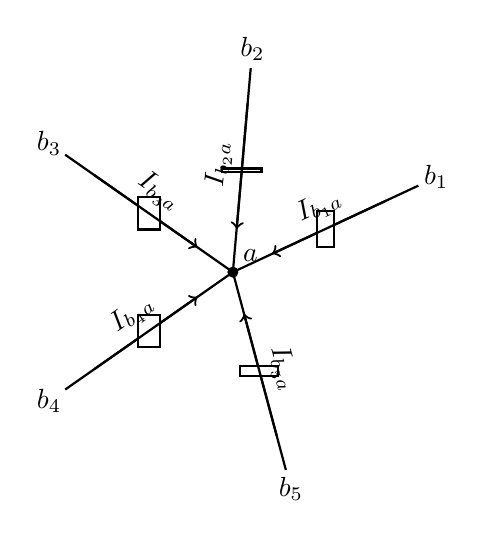
\begin{tikzpicture}[x=1cm,y=1cm,thick]
  \coordinate (a) at (0,0);
  \foreach \ang/\name/\lab in {25/b_1/I_{b_1a},85/b_2/I_{b_2a},145/b_3/I_{b_3a},215/b_4/I_{b_4a},285/b_5/I_{b_5a}} {
    \draw (a)--({2.6*cos(\ang)},{2.6*sin(\ang)});
    \draw[fill=white] ({1.3*cos(\ang)-0.25*sin(\ang)},{1.3*sin(\ang)+0.25*cos(\ang)}) rectangle
      ({1.3*cos(\ang)+0.25*sin(\ang)},{1.3*sin(\ang)-0.25*cos(\ang)});
    \draw[->] ({2.15*cos(\ang)},{2.15*sin(\ang)})--({0.55*cos(\ang)},{0.55*sin(\ang)})
      node[midway,sloped,above] {$\lab$};
    \node at ({2.85*cos(\ang)},{2.85*sin(\ang)}) {$\name$};
  }
  \fill (a) circle (2pt) node[above right] {$a$};
\end{tikzpicture}
}
 \caption{节点 \(a\) 连接若干二端支路 \(b_i a\)。各电流 \(I_{b_i a}\) 都取流入节点 \(a\) 的方向，基尔霍夫第一定律要求它们在每一时刻的代数和为零（原书图 7）。}
 \label{fig:ch2-13-kcl}
\end{figure}

图~\ref{fig:ch2-13-kcl} 表明，电流方程只涉及同一节点的各支路，不涉及节点之间的具体元件类型。若某条支路的参考方向与图中相反，只需把该电流整体变号。

若
\[
 ab,bc,\ldots,hk,ka
\]
依次构成电路中的一个闭合回路，则基尔霍夫第二定律为
\begin{equation}
 U_{ab}(t)+U_{bc}(t)+\cdots+U_{hk}(t)+U_{ka}(t)=0.
 \label{eq:ch2-13-loop-voltage}
\end{equation}

\begin{figure}[H]
 \centering
 \resizebox{0.55\textwidth}{!}{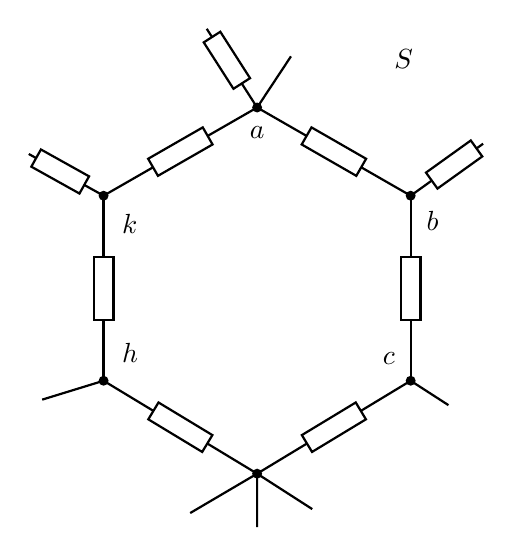
\begin{tikzpicture}[x=1cm,y=1cm,line width=0.8pt]
  \coordinate (a) at (0,2.35);
  \coordinate (b) at (1.95,1.23);
  \coordinate (c) at (1.95,-1.12);
  \coordinate (m) at (0,-2.30);
  \coordinate (h) at (-1.95,-1.12);
  \coordinate (k) at (-1.95,1.23);

  % The unlabelled lower vertex represents intermediate nodes in ab,bc,...,hk,ka.
  \foreach \from/\to in {a/b,b/c,c/m,m/h,h/k,k/a} {
    \draw (\from)--node[midway,sloped,draw,fill=white,
      minimum width=8mm,minimum height=2.5mm,inner sep=0pt]{} (\to);
  }

  % Other branches incident at the loop vertices remain visible.
  \draw (a)--++(0.43,0.65);
  \draw (a)--node[pos=0.60,sloped,draw,fill=white,
    minimum width=7mm,minimum height=2.5mm,inner sep=0pt]{} ++(-0.64,1.00);
  \draw (b)--node[pos=0.60,sloped,draw,fill=white,
    minimum width=7mm,minimum height=2.5mm,inner sep=0pt]{} ++(0.92,0.66);
  \draw (c)--++(0.48,-0.31);
  \draw (m)--++(-0.85,-0.50) (m)--++(0.70,-0.45) (m)--++(0,-0.68);
  \draw (h)--++(-0.78,-0.24);
  \draw (k)--node[pos=0.58,sloped,draw,fill=white,
    minimum width=7mm,minimum height=2.5mm,inner sep=0pt]{} ++(-0.95,0.53);

  \foreach \p in {a,b,c,m,h,k} {\fill (\p) circle (1.8pt);}
  \node[below=3pt] at (a) {$a$};
  \node[below right=2pt] at (b) {$b$};
  \node[above left=2pt] at (c) {$c$};
  \node[above right=3pt] at (h) {$h$};
  \node[below right=3pt] at (k) {$k$};
  \node at (1.86,2.96) {$S$};
\end{tikzpicture}
}
 \caption{闭合回路 \(a\to b\to c\to h\to k\to a\)。沿所有边的电压降按同一绕行方向相加，总代数和为零（原书图 8）。}
 \label{fig:ch2-13-kvl}
\end{figure}

图~\ref{fig:ch2-13-kvl} 的闭合路径说明，电压定律把沿一条闭合路径的各段电压联系起来。实际列方程时，一旦选定绕行方向，逆着绕行方向的电压就带负号；这与 \eqref{eq:ch2-13-reversed-signs} 完全一致。

若电路由 \(n\) 个二端元件组成，则共有 \(2n\) 个未知时间函数，即每个元件的电流与电压。每个元件的本构关系给出 \(n\) 个方程；基尔霍夫定律再提供 \(n\) 个彼此独立的关系。所得方程中，一部分是微分方程，一部分是有限代数方程。通常先利用基尔霍夫定律消去未知函数，再保留最小数目的独立变量代入本构关系。常见做法有两种。

\begin{enumerate}[label=\arabic*.]
 \item \textbf{回路电流法.} 取电流为基本未知函数。先利用基尔霍夫第一定律，把全部支路电流用最小数目的独立回路电流表示；再用基尔霍夫第二定律，把回路中每段电压按本构关系换成相应的电流表达式。
 \item \textbf{节点电压法.} 取电压为基本未知函数。先利用基尔霍夫第二定律，把全部电压用最小数目的独立节点电压表示；再利用基尔霍夫第一定律，把每条支路电流按本构关系换成相应的电压表达式。
\end{enumerate}

两种方法都是有限维线性代数中的基选择思想在电路中的应用：独立回路电流是电流约束的基变量，独立节点电压是电压约束的基变量。

\subsection*{二端网络的算子阻抗}

\medskip
\noindent\textbf{命题 (F)：算子阻抗与算子导纳.}
设 \(ab\) 是电阻、电感或电容。记
\begin{equation}
 U_{ab}(t)=U(t),
 \qquad
 I_{ab}(t)=I(t),
 \qquad
 R_{ab}=R,\quad L_{ab}=L,\quad C_{ab}=C.
 \label{eq:ch2-13-generic-element-data}
\end{equation}
除了前面对 \(D=d/dt\) 的记法，还自然引入
\begin{equation}
 \frac1D f(t)=\int f(t)\,\dd t.
 \label{eq:ch2-13-inverse-D}
\end{equation}
其中不定积分的常数反映电容的初始电量。在零初始条件或只研究定态时，可以把它看作普通的逆运算。

三类无源元件的本构关系可以统一写成
\begin{equation}
 U(t)=Z(D)I(t),
 \label{eq:ch2-13-impedance-law}
\end{equation}
其中
\begin{equation}
 Z_R(D)=R,
 \qquad
 Z_L(D)=LD,
 \qquad
 Z_C(D)=\frac1{CD}.
 \label{eq:ch2-13-element-impedances}
\end{equation}
函数 \(Z(D)\) 称为二端网络的\emph{算子阻抗}。电阻和电感的阻抗是 \(D\) 的多项式，电容的阻抗是有理函数。对电容方程也可写成
\begin{equation}
 U(t)=\frac1{CD}I(t),
 \label{eq:ch2-13-capacitor-impedance}
 \end{equation}
两边乘以 \(CD\) 就回到 \(I=C DU\)。

若 \(Z(D)\) 可逆，则令
\begin{equation}
 G(D)=\frac1{Z(D)},
 \label{eq:ch2-13-admittance-definition}
\end{equation}
并把 \eqref{eq:ch2-13-impedance-law} 改写成
\begin{equation}
 I(t)=G(D)U(t).
 \label{eq:ch2-13-admittance-law}
\end{equation}
\(G(D)\) 称为\emph{算子导纳}。对三种基本元件，
\[
 G_R(D)=\frac1R,
 \qquad
 G_L(D)=\frac1{LD},
 \qquad
 G_C(D)=CD.
\]

图~\ref{fig:ch2-13-terminal-impedance} 用一个方块表示二端网络只看端点时可以观察到的关系。其内部结构不必出现在端点方程中，端点行为已由算子阻抗 \(Z(D)\) 概括。

\begin{figure}[H]
 \centering
 \resizebox{0.62\textwidth}{!}{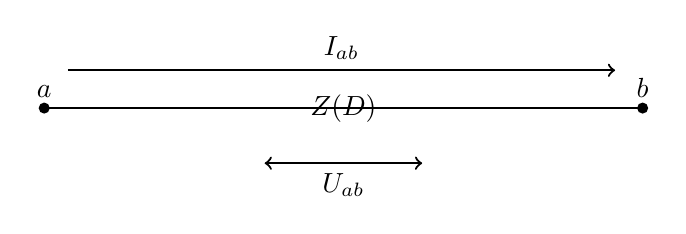
\begin{tikzpicture}[x=1cm,y=1cm,thick]
  \draw (-3.8,0)--(-1.0,0); \draw (1.0,0)--(3.8,0);
  \draw[fill=white,minimum width=2cm,minimum height=0.8cm] (-1,0) rectangle (1,0);
  \node at (0,0) {$Z(D)$};
  \fill (-3.8,0) circle (2pt) node[above] {$a$}; \fill (3.8,0) circle (2pt) node[above] {$b$};
  \draw[->] (-3.5,0.48)--(3.45,0.48) node[midway,above] {$I_{ab}$};
  \draw[<->] (-1.0,-0.7)--(1.0,-0.7) node[midway,below] {$U_{ab}$};
\end{tikzpicture}
}
 \caption{二端网络的端点模型：电流 \(I_{ab}\) 从左端 \(a\) 流向右端 \(b\)，端点电压降为 \(U_{ab}\)，端点本构关系可写成 \(U_{ab}=Z(D)I_{ab}\)（原书图 9）。}
 \label{fig:ch2-13-terminal-impedance}
\end{figure}

对互感，算子记法下的关系为
\begin{align}
 U_1(t)&=L_1D I_1(t)+MD I_2(t),
 \label{eq:ch2-13-mutual-operator-first}\\
 U_2(t)&=L_2D I_2(t)+MD I_1(t).
 \label{eq:ch2-13-mutual-operator-second}
\end{align}

实际的电路常用图表示：用点表示节点，用线段或曲线表示二端元件，在线上标记元件的约定符号。

\begin{figure}[H]
 \centering
 \resizebox{0.42\textwidth}{!}{\begin{tikzpicture}[x=1cm,y=1cm,line width=0.8pt]
  % Resistor.
  \draw (0,7.40)--(0.55,7.40) (2.00,7.40)--(2.55,7.40);
  \draw (0.55,7.25) rectangle (2.00,7.55);
  \node[above=2pt] at (1.28,7.55) {$R$};
  \node[right] at (2.95,7.40) {电阻};

  % The inductor is a sequence of upper semicircles.
  \draw (0,6.43)--(0.38,6.43);
  \draw (0.38,6.43)
    arc[start angle=180,end angle=0,radius=0.18]
    arc[start angle=180,end angle=0,radius=0.18]
    arc[start angle=180,end angle=0,radius=0.18]
    arc[start angle=180,end angle=0,radius=0.18]
    arc[start angle=180,end angle=0,radius=0.18]
    --(2.55,6.43);
  \node[above=2pt] at (1.28,6.61) {$L$};
  \node[right] at (2.95,6.43) {电感};

  % Two separate vertical windings and the coupling arch.
  \draw (0.88,5.69)--(0.88,5.49)
    arc[start angle=90,end angle=270,radius=0.14]
    arc[start angle=90,end angle=270,radius=0.14]
    arc[start angle=90,end angle=270,radius=0.14]
    arc[start angle=90,end angle=270,radius=0.14]
    --(0.88,4.15);
  \draw (1.90,5.69)--(1.90,5.49)
    arc[start angle=90,end angle=-90,radius=0.14]
    arc[start angle=90,end angle=-90,radius=0.14]
    arc[start angle=90,end angle=-90,radius=0.14]
    arc[start angle=90,end angle=-90,radius=0.14]
    --(1.90,4.15);
  \draw (1.05,5.60)..controls (1.25,5.76) and (1.53,5.76)..(1.73,5.60);
  \node[left=4pt] at (0.74,4.91) {$L_1$};
  \node[right=4pt] at (2.04,4.91) {$L_2$};
  \node[right] at (2.95,4.91) {互感};

  % Capacitor plates are separated by a genuine gap.
  \draw (0,3.67)--(1.05,3.67) (1.35,3.67)--(2.55,3.67);
  \draw[line width=2pt] (1.05,3.36)--(1.05,3.98)
    (1.35,3.36)--(1.35,3.98);
  \node[above right=1pt] at (1.35,3.85) {$C$};
  \node[right] at (2.95,3.67) {电容};

  % Source conventions in the original: negative left, positive right.
  \draw (0,2.60)--(1.05,2.60) (1.38,2.60)--(2.55,2.60);
  \draw (1.05,2.42)--(1.05,2.78) (1.38,2.24)--(1.38,2.96);
  \node[above=1pt] at (0.86,2.78) {$-$};
  \node[above=1pt] at (1.67,2.78) {$+$};

  \draw (0,1.65)--(0.84,1.65) (1.66,1.65)--(2.55,1.65);
  \fill (0.84,1.65) circle (2.4pt);
  \fill (1.66,1.65) circle (2.4pt);
  \node at (1.25,1.65) {$\sim$};

  \draw (0,0.60)--(0.84,0.60) (1.70,0.60)--(2.55,0.60);
  \draw (1.27,0.60) circle (0.43);
  \node at (1.27,0.60) {$U(t)$};
  \node[above=1pt] at (0.63,0.83) {$-$};
  \node[above=1pt] at (1.91,0.83) {$+$};

  % Hand-drawn brace; this figure needs no additional TikZ library.
  \draw (2.72,3.06)..controls (2.93,3.06) and (2.94,2.84)..(2.94,2.61)
    --(2.94,2.09)..controls (2.94,1.88) and (3.02,1.83)..(3.13,1.78)
    ..controls (3.02,1.73) and (2.94,1.68)..(2.94,1.47)
    --(2.94,0.77)..controls (2.94,0.49) and (2.91,0.19)..(2.72,0.19);
  \node[right,align=left] at (3.24,1.78) {不变的、简谐的和\\任意变动的电压源};
\end{tikzpicture}
}
 \caption{电路元件的约定记号：电阻、电感、互感、电容，以及不变、简谐和任意变动的电压源。符号只规定元件的支路关系，不规定实际电流的正负（原书图 10）。}
 \label{fig:ch2-13-symbols}
\end{figure}

图~\ref{fig:ch2-13-symbols} 中的符号用于下面三个例子。图形本身不是方程；列方程时仍须结合箭头、正负号和所选绕行方向。

\subsection*{例题 1：振荡回路}

设电路 \(S\) 有四个节点 \(a,b,c,d\)，由四个二端元件
\[
 ab,\quad bc,\quad cd,\quad da
\]
组成。元件 \(ab\) 是电感 \(L\)，\(bc\) 是电阻 \(R\)，\(cd\) 是电容 \(C\)，\(da\) 是电压源 \(U_{da}(t)=-U(t)\)，等价地 \(U_{ad}(t)=U(t)\)。

\begin{figure}[H]
 \centering
 \resizebox{0.48\textwidth}{!}{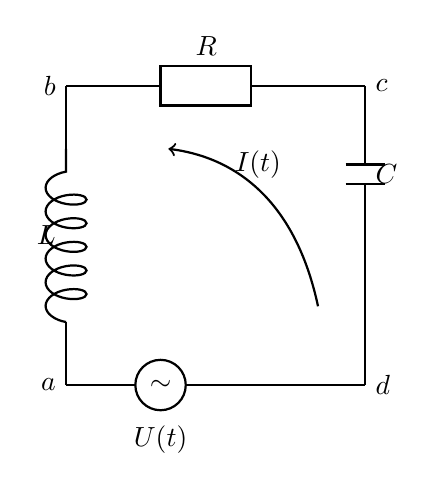
\begin{tikzpicture}[x=1cm,y=1cm,thick]
  \draw (0,0)--(0,0.8); \draw[decorate,decoration={coil,segment length=3mm,amplitude=2.6mm}] (0,0.8)--(0,3.0); \draw (0,3.0)--(0,3.8);
  \draw (0,3.8)--(1.2,3.8); \draw[fill=white] (1.2,3.55) rectangle (2.35,4.05); \node[above] at (1.78,4.05) {$R$}; \draw (2.35,3.8)--(3.8,3.8);
  \draw (3.8,3.8)--(3.8,2.8); \draw (3.55,2.8)--(4.05,2.8); \draw (3.55,2.55)--(4.05,2.55); \draw (3.8,2.55)--(3.8,0);
  \draw (0,0)--(0.88,0); \draw (1.2,0) circle (0.32); \draw (1.52,0)--(3.8,0);
  \node at (1.2,0) {$\sim$};
  \node[left] at (0,0) {$a$}; \node[left] at (0,3.8) {$b$}; \node[right] at (3.8,3.8) {$c$}; \node[right] at (3.8,0) {$d$};
  \node[left] at (0,1.9) {$L$}; \node[right] at (3.8,2.68) {$C$}; \node[below] at (1.2,-0.38) {$U(t)$};
  \draw[->] (3.2,1.0) .. controls (2.9,2.4) and (2.1,2.9) .. (1.3,3.0) node[midway,above] {$I(t)$};
\end{tikzpicture}
}
 \caption{由电感 \(L\)、电阻 \(R\)、电容 \(C\) 和电压源 \(U(t)\) 串联组成的回路；回路中只有一条独立电流，记为 \(I(t)\)（原书图 11）。}
 \label{fig:ch2-13-oscillator-circuit}
\end{figure}

采用回路电流法。在节点 \(b\) 应用基尔霍夫第一定律，有
\begin{equation}
 I_{ab}(t)+I_{cb}(t)=0;
\end{equation}
按参考方向写成常用形式就是 \(I_{ab}(t)=I_{bc}(t)\)。在只有两个二端元件相接的节点处都会得到这类等式。于是四个元件中的电流都相同，记为回路电流 \(I(t)\)：
\begin{equation}
 I_{ab}(t)=I_{bc}(t)=I_{cd}(t)=I_{da}(t)=I(t).
 \label{eq:ch2-13-loop-current}
\end{equation}

对四个元件应用本构关系：
\begin{equation}
 \left\{
 \begin{aligned}
  U_{ab}(t)&=LDI(t),\\
  U_{bc}(t)&=RI(t),\\
  U_{cd}(t)&=\frac1{CD}I(t),\\
  U_{da}(t)&=-U(t).
 \end{aligned}
 \right.
 \label{eq:ch2-13-oscillator-element-voltages}
\end{equation}
沿整个回路应用基尔霍夫第二定律：
\begin{equation}
 U_{ab}(t)+U_{bc}(t)+U_{cd}(t)+U_{da}(t)=0.
 \label{eq:ch2-13-oscillator-kvl}
\end{equation}
代入上面各式，得
\begin{equation}
 \left(LD+R+\frac1{CD}\right)I(t)=U(t).
 \label{eq:ch2-13-oscillator-impedance}
\end{equation}
这是用算子阻抗写出的串联回路方程。两边乘以 \(D\)，就得到不含逆算子的微分方程
\begin{equation}
 \left(LD^2+RD+\frac1C\right)I(t)=DU(t).
 \label{eq:ch2-13-oscillator-differential}
\end{equation}

如果从回路中除去有源元件 \(da\)，就得到断开的无源电路，它由 \(ab,bc,cd\) 三个二端元件串联组成，回路端点 \(a,d\) 之间可整体看成一个二端网络。

\begin{figure}[H]
 \centering
 \resizebox{0.56\textwidth}{!}{\begin{tikzpicture}[x=1cm,y=1cm,thick]
  \draw (0,0)--(0.8,0); \draw[decorate,decoration={coil,segment length=2.8mm,amplitude=2.3mm}] (0.8,0)--(2.1,0); \draw (2.1,0)--(2.3,0);
  \draw (2.3,-0.22) rectangle (3.25,0.22); \node at (2.78,0) {$R$}; \draw (3.25,0)--(3.5,0);
  \draw (3.5,-0.28)--(3.5,0.28); \draw (3.75,-0.28)--(3.75,0.28); \draw (3.75,0)--(4.5,0);
  \fill (0,0) circle (2pt) node[above] {$b$}; \fill (4.5,0) circle (2pt) node[above] {$a$};
  \node[below] at (1.45,-0.05) {$L$}; \node[below] at (3.62,-0.32) {$C$};
  \draw[dashed] (0,-0.72) rectangle (4.5,0.72);
  \node at (2.35,-1.3) {$Z(D)=LD+R+\dfrac{1}{CD}$};
\end{tikzpicture}
}
 \caption{从原回路中移去电压源后，电感、电阻、电容串联形成一个二端网络；其总算子阻抗为 \(Z(D)=LD+R+\frac1{CD}\)（原书图 12）。}
 \label{fig:ch2-13-disconnected-circuit}
\end{figure}

图~\ref{fig:ch2-13-disconnected-circuit} 的端点模型满足
\begin{equation}
 U_{ad}(t)=Z(D)I(t),
 \qquad
 Z(D)=LD+R+\frac1{CD}.
 \label{eq:ch2-13-series-impedance}
\end{equation}
相应的算子导纳为
\begin{equation}
 G(D)=\frac1{Z(D)}
 =\frac{CD}{LCD^2+RCD+1}.
 \label{eq:ch2-13-series-admittance}
\end{equation}

若电源 \(U(t)=0\)，电路由三个无源元件组成，两端点 \(a,d\) 重合。

\begin{figure}[H]
 \centering
 \resizebox{0.45\textwidth}{!}{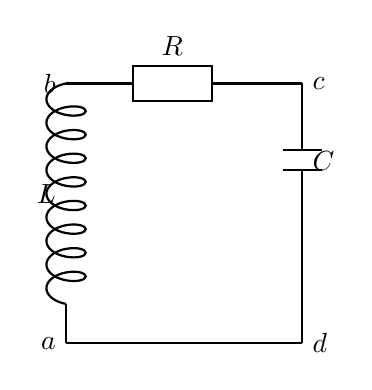
\begin{tikzpicture}[x=1cm,y=1cm,thick]
  \draw (0,0)--(0,0.5); \draw[decorate,decoration={coil,segment length=3mm,amplitude=2.5mm}] (0,0.5)--(0,3.3);
  \draw (0,3.3)--(0.85,3.3); \draw[fill=white] (0.85,3.08) rectangle (1.85,3.52); \node[above] at (1.35,3.52) {$R$}; \draw (1.85,3.3)--(3,3.3);
  \draw (3,3.3)--(3,2.45); \draw (2.75,2.45)--(3.25,2.45); \draw (2.75,2.2)--(3.25,2.2); \draw (3,2.2)--(3,0);
  \draw (0,0)--(3,0); \node[left] at (0,0) {$a$}; \node[left] at (0,3.3) {$b$}; \node[right] at (3,3.3) {$c$}; \node[right] at (3,0) {$d$};
  \node[left] at (0,1.9) {$L$}; \node[right] at (3,2.32) {$C$};
\end{tikzpicture}
}
 \caption{无源闭合振荡回路：去除电压源并以导线闭合端点后，支路中仍可存在初始电流；电感、电阻和电容共同决定其自由衰减（原书图 13）。}
 \label{fig:ch2-13-passive-loop}
\end{figure}

图~\ref{fig:ch2-13-passive-loop} 对应方程
\begin{equation}
 \left(LD^2+RD+\frac1C\right)I(t)=0.
 \label{eq:ch2-13-passive-loop-equation}
\end{equation}
无源电路不会自发产生持续电流，零函数是它的特解；但若初始时已有电流或电容已充电，仍可研究这些状态如何随时间演化。特征多项式为
\begin{equation}
 L(s)=Ls^2+Rs+\frac1C.
 \label{eq:ch2-13-loop-characteristic}
\end{equation}
因为 \(L,C>0\)，若 \(R\ge0\)，则所有系数非负且常数项为正；由 §9 命题 (B)，在 \(R>0\) 时它稳定，电流按指数速度衰减。若 \(R=0\)，则为下一段的无阻尼理想情形。

为区分衰减方式，计算判别式
\begin{equation}
 \Delta=\left(\frac{R}{2L}\right)^2-\frac1{LC}.
 \label{eq:ch2-13-loop-discriminant}
\end{equation}
若 \(\Delta<0\)，两个特征根为共轭复数，非零解具有振动特性；若 \(\Delta>0\)，两个根都是负实数，非周期地衰减。\(\Delta=0\) 是退化边界，此时有负二重根
\[
 \lambda=-\frac{R}{2L},
\]
解含因子 \(1,t\)，仍不振荡且当 \(t\to+\infty\) 时趋于零。无论 \(\Delta\) 属于哪一种，只有 \(\Delta<0\) 时才会在衰减包络下反复改变符号。

特别考虑完全没有电阻的振荡回路。此时电路只剩电感 \(ab\) 与电容 \(cd\)，并且端点满足 \(b=c,a=d\)。

\begin{figure}[H]
 \centering
 \resizebox{0.34\textwidth}{!}{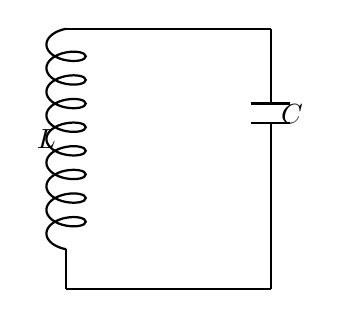
\begin{tikzpicture}[x=1cm,y=1cm,thick]
  \draw (0,0)--(0,0.5); \draw[decorate,decoration={coil,segment length=3mm,amplitude=2.5mm}] (0,0.5)--(0,3.3);
  \draw (0,3.3)--(2.6,3.3); \draw (2.6,3.3)--(2.6,2.35); \draw (2.35,2.35)--(2.85,2.35); \draw (2.35,2.1)--(2.85,2.1); \draw (2.6,2.1)--(2.6,0); \draw (0,0)--(2.6,0);
  \node[left] at (0,1.9) {$L$}; \node[right] at (2.6,2.22) {$C$};
\end{tikzpicture}
}
 \caption{无电阻的理想 LC 回路。电感与电容直接把能量相互转换，既不耗散也不产生能量，因此得到频率为 \(1/\sqrt{LC}\) 的非衰减振荡（原书图 14）。}
 \label{fig:ch2-13-lc-loop}
\end{figure}

图~\ref{fig:ch2-13-lc-loop} 的回路方程为
\begin{equation}
 \left(LD^2+\frac1C\right)I(t)=0,
 \label{eq:ch2-13-lc-equation}
\end{equation}
或
\begin{equation}
 \left(D^2+\frac1{LC}\right)I(t)=0.
 \label{eq:ch2-13-lc-normalized}
\end{equation}
通解为
\begin{equation}
 I(t)=s\cos(\omega_1t+\beta),
 \qquad
 \omega_1=\frac1{\sqrt{LC}},
 \label{eq:ch2-13-lc-solution}
\end{equation}
其中 \(s,\beta\) 是实常数。量
\[
 \omega_1=\frac1{\sqrt{LC}}
\]
称为振荡回路的固有角频率；没有电阻时，它与振幅无关，振荡永不衰减。

再回到包含简谐电压源的回路。若
\begin{equation}
 U(t)=re^{i\omega t},
 \qquad r>0,
 \label{eq:ch2-13-harmonic-loop-source}
\end{equation}
那么由 \eqref{eq:ch2-13-oscillator-differential}，
\begin{equation}
 DU(t)=ir\omega e^{i\omega t}.
 \label{eq:ch2-13-source-derivative}
\end{equation}
设定态电流为
\[
 I_{\mathrm{ss}}(t)=\sigma e^{i\omega t}.
\]
在 \eqref{eq:ch2-13-oscillator-impedance} 中取 \(D=i\omega\)，得到
\begin{align}
 \sigma
 &=\frac{ir\omega}
 {iR\omega+\left(-L\omega^2+\frac1C\right)}\notag\\
 &=\frac{r}{R+i\left(L\omega-\frac1{C\omega}\right)}.
 \label{eq:ch2-13-loop-complex-amplitude}
\end{align}
因此定态电流的实振幅为
\begin{equation}
 s=|\sigma|
 =\frac{r}
 {\sqrt{R^2+\left(L\omega-\frac1{C\omega}\right)^2}}.
 \label{eq:ch2-13-loop-amplitude}
\end{equation}
对固定振幅 \(r\) 的电源，当
\begin{equation}
 L\omega-\frac1{C\omega}=0,
 \qquad
 \omega=\frac1{\sqrt{LC}}=\omega_1
 \label{eq:ch2-13-loop-resonance}
\end{equation}
时分母最小，电流振幅达到最大值
\[
 s=\frac rR.
\]
也就是说，在共振频率处，回路表现得好似只有电阻 \(R\) 存在。对其他频率，振幅都小于 \(r/R\)。这就是 RLC 振荡回路的共振现象。

\subsection*{例题 2：变压器}

变压器由安装在同一铁芯上的原绕组和副绕组构成。原绕组接可变电压源，副绕组接负载，例如外电阻。每个绕组都有电感和内电阻；两个绕组之间还有互感。因此可把变压器看成两个通过互感耦合的回路。

\begin{figure}[H]
 \centering
 \resizebox{0.68\textwidth}{!}{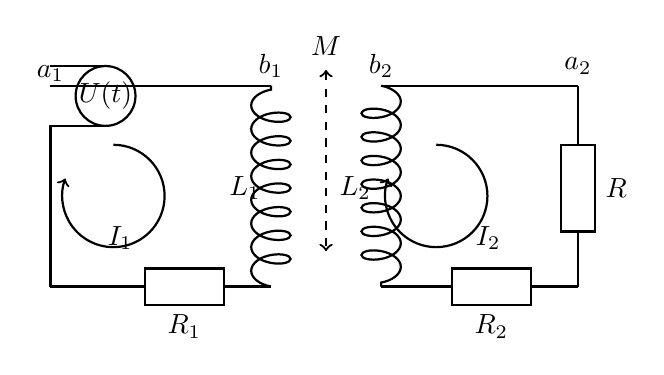
\begin{tikzpicture}[x=1cm,y=1cm,thick]
  % Coupled primary and secondary loops with distinct current arrows.
  \draw (0,0)--(0.7,0); \draw (0.7,-0.38) circle (0.38); \node at (0.7,-0.38) {$U(t)$}; \draw (0.7,-0.76)--(0,-0.76)--(0,-2.8);
  \draw (0,-2.8)--(1.2,-2.8); \draw[fill=white] (1.2,-3.03) rectangle (2.2,-2.57); \node[below] at (1.7,-3.03) {$R_1$}; \draw (2.2,-2.8)--(2.8,-2.8);
  \draw[decorate,decoration={coil,segment length=3mm,amplitude=2.5mm}] (2.8,-2.8)--(2.8,-0.25); \draw (2.8,-0.25)--(0,-0.25);
  \draw (4.2,-0.25)--(6.7,-0.25); \draw[decorate,decoration={coil,segment length=3mm,amplitude=2.5mm}] (4.2,-0.25)--(4.2,-2.8); \draw (4.2,-2.8)--(5.1,-2.8);
  \draw[fill=white] (5.1,-3.03) rectangle (6.1,-2.57); \node[below] at (5.6,-3.03) {$R_2$}; \draw (6.1,-2.8)--(6.7,-2.8);
  \draw (6.7,-2.8)--(6.7,-0.25); \draw (6.7,-1.0)--(6.7,-2.1); \draw[fill=white] (6.48,-2.1) rectangle (6.92,-1.0); \node[right] at (6.92,-1.55) {$R$};
  \node[left] at (2.8,-1.55) {$L_1$}; \node[left] at (4.2,-1.55) {$L_2$};
  \node at (3.5,0.25) {$M$}; \draw[<->,dashed] (3.5,-0.05)--(3.5,-2.35);
  \draw[->] (0.8,-1.0) arc[start angle=90,end angle=-200,radius=0.65] node[midway,left] {$I_1$};
  \draw[->] (4.9,-1.0) arc[start angle=90,end angle=-200,radius=0.65] node[midway,right] {$I_2$};
  \node at (0,-0.1) {$a_1$}; \node at (2.8,0) {$b_1$}; \node at (4.2,0) {$b_2$}; \node at (6.7,0) {$a_2$};
\end{tikzpicture}
}
 \caption{互感耦合的变压器模型：原边回路含电源 \(U(t)\)、电感 \(L_1\) 和内电阻 \(R_1\)，副边回路含电感 \(L_2\)、内电阻 \(R_2\) 与负载电阻 \(R\)，两电感以 \(M\) 耦合（原书图 15）。}
 \label{fig:ch2-13-transformer}
\end{figure}

图~\ref{fig:ch2-13-transformer} 中第一个回路有三个二端元件：电感 \(L_1\)、内电阻 \(R_1\) 和电压源 \(U(t)\)。第二个回路也有三个：电感 \(L_2\)、内电阻 \(R_2\) 和负载电阻 \(R\)。此外还有互感
\[
 M=M_{a_1b_1,a_2b_2}.
\]
设两个回路电流分别为 \(I_1,I_2\)。在每个只有两个元件相接的节点处应用基尔霍夫第一定律，可知同一绕组回路中的所有支路电流相同。于是两个回路的回路电流正是 \(I_1,I_2\)。

对两个回路应用基尔霍夫第二定律并代入互感本构关系，得到
\begin{align}
 L_1DI_1+MDI_2+R_1I_1-U(t)&=0,
 \label{eq:ch2-13-transformer-loop1}\\
 L_2DI_2+MDI_1+R_2I_2+RI_2&=0.
 \label{eq:ch2-13-transformer-loop2}
\end{align}
整理成标准形式：
\begin{align}
 (L_1D+R_1)I_1+MDI_2&=U(t),
 \label{eq:ch2-13-transformer-system1}\\
 MDI_1+(L_2D+R_2+R)I_2&=0.
 \label{eq:ch2-13-transformer-system2}
\end{align}

系数矩阵的行列式为
\begin{align}
 D_{\mat{L}}(s)
 &=(L_1s+R_1)(L_2s+R_2+R)-M^2s^2\notag\\
 &=(L_1L_2-M^2)s^2
   +\bigl(L_1(R_2+R)+R_1L_2\bigr)s
   +R_1(R_2+R).
 \label{eq:ch2-13-transformer-determinant}
\end{align}
由 \(M^2<L_1L_2\) 以及正的电阻值，三个系数都为正。它是二次实多项式，由 §9 命题 (B)，稳定；因此自由响应随时间衰减，可以讨论唯一的定态响应。

设原边电压为复简谐函数
\begin{equation}
 U(t)=u_1e^{i\omega t},
 \qquad u_1>0.
 \label{eq:ch2-13-transformer-harmonic-source}
\end{equation}
寻找
\begin{equation}
 I_1(t)=\sigma_1e^{i\omega t},
 \qquad
 I_2(t)=\sigma_2e^{i\omega t}.
 \label{eq:ch2-13-transformer-complex-currents}
\end{equation}
代入 \eqref{eq:ch2-13-transformer-system1}--\eqref{eq:ch2-13-transformer-system2}，约去 \(e^{i\omega t}\)：
\begin{align}
 (iL_1\omega+R_1)\sigma_1+iM\omega\sigma_2&=u_1,
 \label{eq:ch2-13-transformer-phasors1}\\
 iM\omega\sigma_1+(iL_2\omega+R_2+R)\sigma_2&=0.
 \label{eq:ch2-13-transformer-phasors2}
\end{align}

理论分析中最重要的是理想变压器极限：内电阻 \(R_1,R_2\) 以及漏感量 \(L_1L_2-M^2\) 都很小。忽略这些小量后，
\begin{align}
 iL_1\omega\sigma_1+iM\omega\sigma_2&=u_1,
 \label{eq:ch2-13-ideal-transformer1}\\
 iM\omega\sigma_1+(iL_2\omega+R)\sigma_2&=0.
 \label{eq:ch2-13-ideal-transformer2}
\end{align}
此时 \(M\approx\sqrt{L_1L_2}\)。把第一式乘以 \(\sqrt{L_2/L_1}\)，再减去第二式，第一组中的 \(\sigma_1\) 项因
\[
 \sqrt{\frac{L_2}{L_1}}\,L_1=\sqrt{L_1L_2}\approx M
\]
而抵消，得到
\begin{equation}
 R\sigma_2=-\sqrt{\frac{L_2}{L_1}}u_1.
 \label{eq:ch2-13-transformer-load-current}
\end{equation}
因此负载 \(R\) 上的电压振幅为
\begin{equation}
 u_2=R|\sigma_2|
 =\sqrt{\frac{L_2}{L_1}}u_1.
 \label{eq:ch2-13-transformer-voltage-ratio}
\end{equation}
比值
\[
 \sqrt{\frac{L_2}{L_1}}
\]
称为变压器的变压系数。若 \(L_2>L_1\)，则 \(u_2/u_1>1\)，这是升压变压器；若 \(L_2<L_1\)，则 \(u_2/u_1<1\)，这是降压变压器。

\subsection*{例题 3：电子滤波器}

考虑有四个节点 \(a,b,c,d\) 和五个二端元件的电路：\(ab\) 是电感 \(L\)，\(bc\) 是具有同样电感 \(L\) 的电感，\(bd\) 是电容 \(C\)，\(ad\) 是电压源 \(U_{ad}(t)=U(t)\)，\(cd\) 是负载电阻 \(R\)。

\begin{figure}[H]
 \centering
 \resizebox{0.72\textwidth}{!}{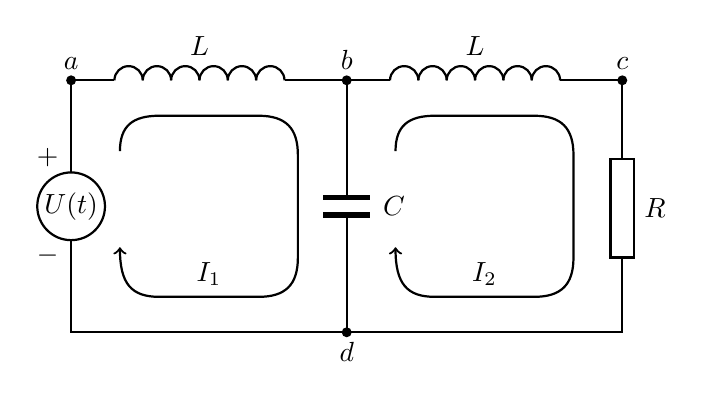
\begin{tikzpicture}[x=1cm,y=1cm,thick]
  % Two series inductors; shunt capacitor bd has a real dielectric gap.
  \draw (0,3.2)--(0.55,3.2);
  \foreach \k in {0,...,5}
    \draw ({0.55+0.36*\k},3.2) arc[start angle=180,end angle=0,radius=0.18];
  \draw (2.71,3.2)--(3.5,3.2)--(4.05,3.2);
  \foreach \k in {0,...,5}
    \draw ({4.05+0.36*\k},3.2) arc[start angle=180,end angle=0,radius=0.18];
  \draw (6.21,3.2)--(7,3.2)--(7,2.2);
  \draw (6.85,0.95) rectangle (7.15,2.2);
  \draw (7,0.95)--(7,0)--(0,0)--(0,1.17);
  \draw (0,1.6) circle (0.43);
  \draw (0,2.03)--(0,3.2);
  \node at (0,1.6) {$U(t)$};
  \node[left] at (-0.03,2.22) {$+$}; \node[left] at (-0.03,0.98) {$-$};
  \draw (3.5,3.2)--(3.5,1.71);
  \draw[line width=2pt] (3.2,1.71)--(3.8,1.71) (3.2,1.49)--(3.8,1.49);
  \draw (3.5,1.49)--(3.5,0);
  \fill (0,3.2) circle (1.8pt) node[above] {$a$};
  \fill (3.5,3.2) circle (1.8pt) node[above] {$b$};
  \fill (7,3.2) circle (1.8pt) node[above] {$c$};
  \fill (3.5,0) circle (1.8pt) node[below] {$d$};
  \node[above] at (1.63,3.38) {$L$}; \node[above] at (5.13,3.38) {$L$};
  \node[right] at (3.83,1.60) {$C$}; \node[right] at (7.15,1.575) {$R$};
  \draw[->] (0.62,2.3)
    .. controls (0.62,2.62) and (0.78,2.75) .. (1.12,2.75)
    --(2.38,2.75)
    .. controls (2.73,2.75) and (2.88,2.59) .. (2.88,2.25)
    --(2.88,0.95)
    .. controls (2.88,0.6) and (2.72,0.45) .. (2.38,0.45)
    --(1.12,0.45)
    .. controls (0.77,0.45) and (0.62,0.61) .. (0.62,1.08);
  \node[above] at (1.75,0.46) {$I_1$};
  \draw[->] (4.12,2.3)
    .. controls (4.12,2.62) and (4.28,2.75) .. (4.62,2.75)
    --(5.88,2.75)
    .. controls (6.23,2.75) and (6.38,2.59) .. (6.38,2.25)
    --(6.38,0.95)
    .. controls (6.38,0.6) and (6.22,0.45) .. (5.88,0.45)
    --(4.62,0.45)
    .. controls (4.27,0.45) and (4.12,0.61) .. (4.12,1.08);
  \node[above] at (5.25,0.46) {$I_2$};
\end{tikzpicture}
}
 \caption{两级 LC 低通滤波器：两个等值电感 \(L\) 分处上支路，电容 \(C\) 跨接在中间节点 \(b\) 与下节点 \(d\) 之间，负载电阻 \(R\) 接在右端；回路电流分别为 \(I_1,I_2\)（原书图 16）。}
 \label{fig:ch2-13-filter}
\end{figure}

图~\ref{fig:ch2-13-filter} 中用两个回路电流 \(I_1,I_2\) 表示支路电流：
\begin{equation}
 I_{ab}=I_1,
 \qquad
 I_{bc}=I_2.
 \label{eq:ch2-13-filter-loop-currents}
\end{equation}
在节点 \(b\) 应用基尔霍夫第一定律，得到
\begin{equation}
 I_{bd}=I_1-I_2,
 \qquad
 I_{cd}=I_2.
 \label{eq:ch2-13-filter-branch-currents}
\end{equation}

沿左侧大回路和右侧回路分别应用基尔霍夫第二定律：
\begin{align}
 U_{ab}+U_{bc}+U_{cd}+U_{da}&=0,
 \label{eq:ch2-13-filter-kvl1}\\
 U_{bc}+U_{cd}+U_{db}&=0.
 \label{eq:ch2-13-filter-kvl2}
\end{align}
代入本构关系：
\begin{align}
 LDI_1+LDI_2+RI_2-U(t)&=0,
 \label{eq:ch2-13-filter-equations1}\\
 LDI_2+RI_2+\frac1{CD}(I_2-I_1)&=0.
 \label{eq:ch2-13-filter-equations2}
\end{align}
把第二式乘以 \(D\)，整理为
\begin{align}
 LDI_1+(LD+R)I_2&=U(t),
 \label{eq:ch2-13-filter-system1}\\
 -\frac1C I_1+\left(LD^2+RD+\frac1C\right)I_2&=0.
 \label{eq:ch2-13-filter-system2}
\end{align}

系数矩阵的行列式为
\begin{equation}
 D_{\mat{L}}(s)
 =L^2s^3+LRs^2+\frac{2L}{C}s+\frac{R}{C}.
 \label{eq:ch2-13-filter-determinant}
\end{equation}
它的首项系数为正，所有系数都为正，并且
\[
 (LR)\left(\frac{2L}{C}\right)
 > L^2\left(\frac{R}{C}\right).
\]
由定理 6，三次多项式 \(D_{\mat{L}}(s)\) 稳定。因此滤波器存在稳定定态。

研究复简谐输入
\begin{equation}
 U(t)=be^{i\omega t},
 \qquad b>0,
 \label{eq:ch2-13-filter-input}
\end{equation}
并设
\begin{equation}
 I_1(t)=\alpha_1e^{i\omega t},
 \qquad
 I_2(t)=\alpha_2e^{i\omega t}.
 \label{eq:ch2-13-filter-complex-currents}
\end{equation}
在 \eqref{eq:ch2-13-filter-system1}--\eqref{eq:ch2-13-filter-system2} 中取 \(D=i\omega\)，可先由第二式得到
\begin{equation}
 \alpha_1
 =C\left(-L\omega^2+iR\omega+\frac1C\right)\alpha_2.
 \label{eq:ch2-13-filter-alpha1}
\end{equation}
再代回第一式并解出
\begin{equation}
 \alpha_2=
 \frac{b/C}
 {\left(\frac RC-LR\omega^2\right)
  +i\omega\left(\frac{2L}{C}-L^2\omega^2\right)}.
 \label{eq:ch2-13-filter-alpha2}
\end{equation}

负载电阻上的电压降为 \(U_{cd}=RI_2\)，其振幅为
\begin{equation}
 a=|\alpha_2|R
 =\frac{bR/C}
 {\sqrt{\left(\frac RC-LR\omega^2\right)^2
 +\omega^2\left(\frac{2L}{C}-L^2\omega^2\right)^2}}.
 \label{eq:ch2-13-filter-output-amplitude}
\end{equation}
因此
\begin{equation}
 \frac ab
 =\frac{R/C}
 {\sqrt{\left(\frac RC-LR\omega^2\right)^2
 +\omega^2\left(\frac{2L}{C}-L^2\omega^2\right)^2}}.
 \label{eq:ch2-13-filter-transfer}
\end{equation}

当频率 \(\omega\) 很小时，分母近似为 \(R/C\)，所以
\[
 \frac ab\approx1.
\]
低频电压几乎原样传到负载。当频率很大时，分母主项由
\(LR\omega^2\) 与 \(L^2\omega^3/C\) 给出，其中三次项占主导，因而
\begin{equation}
 \frac ab\approx\frac{R}{CL^2\omega^3}.
 \label{eq:ch2-13-filter-high-frequency}
\end{equation}
比值迅速趋近于零，高频信号几乎不能通过。于是这个电路表现为低通滤波器：低频容易通过，高频被“滤掉”。这里的“稳定”“定态”“滤掉”都是对上述理想线性模型而言；真实滤波器还受元件寄生效应、负载变化和物理功率限制的影响。

\section{标准的常系数线性齐次方程组}

\newenvironment{sourceitem}[1]
  {\par\medskip\noindent\textbf{#1}\quad\ignorespaces}
  {\par\medskip}

本节讨论常系数线性齐次方程组
\begin{equation}
 x_i'=\sum_{j=1}^{n}a_{ij}x_j,\qquad i=1,\ldots,n,
 \tag{1}
\end{equation}
其中 \(\mat{A}=(a_{ij})\in\R^{n\times n}\)。把未知函数排成列向量
\[
 \vect{x}(t)=
 \begin{pmatrix}
  x_1(t)\\
  \vdots\\
  x_n(t)
 \end{pmatrix},
\]
方程组便写成标准的向量形式
\begin{equation}
 \vect{x}'=\mat{A}\vect{x}.
 \tag{2}
\end{equation}
这里 \(\vect{x}'(t)\) 是逐分量求导所得的列向量。以后若不另作说明，\(\mat{A}\) 的元素均为实常数；
讨论复特征向量时，使用复向量空间 \(\C^n\)，但最终仍要从中分出实解。

这个方程组当然可以用消去法求解，即将它写成多项式矩阵方程并利用第~\S11 中的消元程序；
本节采用另一种组织方式：研究 \(\mat{A}\) 的特征向量、广义特征向量和 Jordan 链。若 \(\mat{A}\) 有
\(n\) 个互不相同的特征值，则存在由特征向量组成的基，把 \(\mat{A}\) 对角化。这一步只依赖
线性代数的基本结论，这种谱称为简单谱。若 \(\mat{A}\) 有重特征值而不能对角化，则一般
Jordan 标准形需要较完整
的线性代数证明；本书后面的内容并不要求读者先掌握一般 Jordan 标准形的构造。本节仍把
相应结论写入命题 (C)、(D)、(G)，以便说明通解为何具有 \(t^k e^{\lambda t}\) 的形状，
并保证关于常系数线性系统的叙述完整。只关心单特征值情形的读者可以先读到命题 (F)，再
继续后面各节；Jordan 链部分不成为后续相平面讨论的必要前提。

把矩阵化为 Jordan 标准形，通常伴随未知函数的线性变换。本节末尾的“变量的变换”会系统
说明这一点。本节的直接构造则先以特征向量和 Jordan 链给出基本解，实际上仍是标准形思想
的坐标表述。

本节在固定标准基下暂时不再区分矩阵 \(\mat{A}\) 与它表示的线性算子，因为大部分公式不需要换基。
只在命题 (F) 中选取特征向量基时，才有必要区分算子与它在不同基底下的矩阵。若把 \(\mat{A}\)
看成 \(T_{\mat{A}}:\R^n\to\R^n\)，那么 \(\mat{A}\vect{h}=\lambda \vect{h}\) 就是 \(T_{\mat{A}}\vect{h}=\lambda \vect{h}\) 的矩阵写法。

\subsection*{特征方程的根全是单根的情形}
\addcontentsline{toc}{subsection}{特征方程的根全是单根的情形}

\begin{sourceitem}{命题 (A)}
设 \(\vect{h}\in\C^n\setminus\{\vect{0}\}\) 是 \(\mat{A}\) 对应于特征值 \(\lambda\) 的特征向量，即
\begin{equation}
 \mat{A}\vect{h}=\lambda \vect{h}.
 \tag{3}
\end{equation}
则向量函数
\begin{equation}
 \vect{x}(t)=\vect{h}\,e^{\lambda t}
 \tag{4}
\end{equation}
是方程 \(\vect{x}'=\mat{A}\vect{x}\) 的解。
\end{sourceitem}

把命题 (A) 中的候选函数直接代入即可：
\[
 \vect{x}'(t)=\lambda \vect{h} e^{\lambda t},\qquad
 \mat{A}\vect{x}(t)=\mat{A} \vect{h} e^{\lambda t}=\lambda \vect{h} e^{\lambda t}.
\]
这里真正用到的是 \(\vect{h}\neq\vect{0}\)。若 \(\vect{h}=\vect{0}\)，公式虽然给出零解，却不能把任何方向标成特征
方向。由线性性，若干个这样的解相加仍然给出解。关键问题是这些解是否已经覆盖了全部解。

\begin{sourceitem}{定理 10}
设
\begin{equation}
 \vect{x}'=\mat{A}\vect{x}
 \tag{5}
\end{equation}
中的矩阵 \(\mat{A}\) 有 \(n\) 个两两不同的特征值
\[
 \lambda_1,\lambda_2,\ldots,\lambda_n,
\]
并设 \(\vect{h}_1,\ldots,\vect{h}_n\) 分别是与它们对应的特征向量。令
\begin{equation}
 \vect{x}_i(t)=\vect{h}_i e^{\lambda_i t},\qquad i=1,\ldots,n,
 \tag{6}
\end{equation}
则
\begin{equation}
 \vect{x}(t)=c_1\vect{x}_1(t)+\cdots+c_n\vect{x}_n(t)
   =\sum_{i=1}^{n}c_i \vect{h}_i e^{\lambda_i t}
 \tag{7}
\end{equation}
是方程 (5) 的解，其中 \(c_1,\ldots,c_n\) 为任意常数；并且方程
(5) 的每一个解都可以写成式 (7) 的形式。
\end{sourceitem}

由命题 (A)，每一个 \(\vect{x}_i\) 都是方程的解；由齐次线性方程组的叠加原理，任意线性组合
式 (7) 仍是解。下面证明没有遗漏。

设 \(\vect{\varphi}(t)\) 是方程的任一解。根据常系数线性系统解的整体存在唯一性，可以把它的
定义区间延拓为整个实轴，因此 \(\vect{\varphi}(0)\) 有意义。记
\[
 \vect{x}_0=\vect{\varphi}(0).
\]
因为属于不同特征值的特征向量线性无关，而这里恰有 \(n\) 个，所以
\(\vect{h}_1,\ldots,\vect{h}_n\) 构成 \(\C^n\) 的一组基。于是可唯一写出
\begin{equation}
 \vect{x}_0=c_1\vect{h}_1+\cdots+c_n\vect{h}_n.
 \tag{8}
\end{equation}
由定义 \(\vect{x}_i(0)=\vect{h}_i\)，由式 (7) 定义的解满足
\[
 \vect{x}(0)=\sum_{i=1}^{n}c_i\vect{h}_i=\vect{x}_0.
\]
因此 \(\vect{x}(t)\) 与 \(\vect{\varphi}(t)\) 具有相同初始值。由初值问题解的唯一性，
\(\vect{\varphi}(t)=\vect{x}(t)\)。这就证明了定理 10。

当 \(\mat{A}\) 是实矩阵时，定理 10 的复解公式还不是实解公式。实矩阵的复特征值成共轭对出现，
但若任意选取复特征向量，所得基中的复共轭关系也可能不整齐。通常按下列方式选基。

\begin{sourceitem}{命题 (B)}
设 \(\mat{A}\) 是实矩阵，并选取特征向量基 \(\vect{h}_1,\ldots,\vect{h}_n\)，使实特征值对应实特征向量，
使复共轭特征值 \(\lambda\) 与 \(\overline\lambda\) 对应复共轭特征向量
\(\vect{h}\) 与 \(\overline{\vect{h}}\)。那么公式 (7) 是实解，当且仅当实特征值所对
应的系数取实常数，而每一对复共轭解所对应的系数取彼此复共轭的常数。
\end{sourceitem}

原因是实矩阵把 \(\overline{\vect{h}}\) 送到与 \(\overline\lambda\) 对应的特征向量，而
\(e^{\overline\lambda t}=\overline{e^{\lambda t}}\)。只要系数按共轭方式配对，对
式 (7) 取共轭后所得向量函数仍等于它自身，故解为实值。这一点与
第~\S7 中实系数方程分离实解的命题完全一致。反过来，若组合为实值，按复特征基坐标的
唯一性，实特征向量前的系数与复共轭特征向量前的系数也必须按同样方式配对。

\subsection*{一般情形与 Jordan 链}
\addcontentsline{toc}{subsection}{一般情形与 Jordan 链}

现在允许 \(\mat{A}\) 有重特征值。若 \(\mat{A}\) 不能对角化，单靠 \(e^{\lambda t}\vect{h}\) 不足以产生
全部解；Jordan 链会补充 \(t e^{\lambda t},t^2e^{\lambda t},\ldots\) 这类项。先取一个
固定特征值 \(\lambda\)，设
\begin{equation}
 \vect{h}_1,\ldots,\vect{h}_k
 \tag{9}
\end{equation}
是 \(\mat{A}\) 关于 \(\lambda\) 的一条 Jordan 链，即
\begin{equation}
 \mat{A}\vect{h}_1=\lambda \vect{h}_1,\qquad
 \mat{A}\vect{h}_2=\lambda \vect{h}_2+\vect{h}_1,\qquad
 \ldots,\qquad
 \mat{A}\vect{h}_k=\lambda \vect{h}_k+\vect{h}_{k-1}.
 \tag{10}
\end{equation}
这里 \(\vect{h}_1\neq\vect{0}\)，而 \(\vect{h}_2,\ldots,\vect{h}_k\) 一般只是广义特征向量。等价地，
\((\mat{A}-\lambda \mat{I})\vect{h}_1=\vect{0}\)，并且 \((\mat{A}-\lambda \mat{I})\vect{h}_r=\vect{h}_{r-1}\) 对
\(r=2,\ldots,k\) 成立。

\begin{sourceitem}{命题 (C)}
对 \(r=1,\ldots,k\)，定义向量多项式
\begin{equation}
 \vect{w}_r(t)=\frac{t^{r-1}}{(r-1)!}\vect{h}_1
       +\frac{t^{r-2}}{(r-2)!}\vect{h}_2
       +\cdots+\vect{h}_r,
 \tag{11}
\end{equation}
并约定 \(\vect{w}_0(t)=\vect{0}\)。则
\begin{equation}
 \vect{x}_r(t)=\vect{w}_r(t)e^{\lambda t},\qquad r=1,\ldots,k,
 \tag{12}
\end{equation}
都是 \(\vect{x}'=\mat{A}\vect{x}\) 的解，并且
\begin{equation}
 \vect{x}_r(0)=\vect{h}_r.
 \tag{13}
\end{equation}
\end{sourceitem}

先注意两个直接由定义得到的恒等式：
\begin{equation}
 \vect{w}_r'(t)=\vect{w}_{r-1}(t),\qquad
 \mat{A}\vect{w}_r(t)=\lambda \vect{w}_r(t)+\vect{w}_{r-1}(t),
 \qquad r=1,\ldots,k.
 \tag{14}
\end{equation}
第二式在 \(r=1\) 时就是 \(\mat{A}\vect{w}_1=\lambda \vect{w}_1\)，因为 \(\vect{w}_0=\vect{0}\)。于是
\[
 \vect{x}_r'(t)
 =\vect{w}_r'(t)e^{\lambda t}+\lambda \vect{w}_r(t)e^{\lambda t}
 =\bigl(\vect{w}_{r-1}(t)+\lambda \vect{w}_r(t)\bigr)e^{\lambda t},
\]
而
\[
 \mat{A}\vect{x}_r(t)=\mat{A}\vect{w}_r(t)e^{\lambda t}
 =\bigl(\lambda \vect{w}_r(t)+\vect{w}_{r-1}(t)\bigr)e^{\lambda t}.
\]
两边相等，所以 \(\vect{x}_r'=\mat{A}\vect{x}_r\)。在 \(t=0\) 时，\(\vect{w}_r(0)=\vect{h}_r\)，从而
\(\vect{x}_r(0)=\vect{h}_r\)。

若线性算子在某一组基下有多个 Jordan 块，每一块都给出一组如式 (12) 的解。把所有块得到
的解合并，应该得到 \(n\) 个线性无关的解。下面的定理把这一结论写成
不需要单独选择坐标的向量形式。

\begin{sourceitem}{定理 11}
设 \(\vect{x}'=\mat{A}\vect{x}\)。存在由若干条 Jordan 链组成的基
\begin{equation}
 \vect{h}_1,\ldots,\vect{h}_n.
 \tag{15}
\end{equation}
按特征值把各链分组；为确定记号，假设
\[
 \vect{h}_1,\ldots,\vect{h}_{k_1}
\]
是关于 \(\lambda_1\) 的一条链，
\[
 \vect{h}_{k_1+1},\ldots,\vect{h}_{k_1+k_2}
\]
是关于 \(\lambda_2\) 的一条链，余此类推。每一组链都按命题 (C) 生成对应的解。把所得
\(n\) 个解记为 \(\vect{x}_1,\ldots,\vect{x}_n\)。则
\begin{equation}
 \vect{x}(t)=c_1\vect{x}_1(t)+\cdots+c_n\vect{x}_n(t)
 \tag{16}
\end{equation}
总是方程 \(\vect{x}'=\mat{A}\vect{x}\) 的解，其中 \(c_1,\ldots,c_n\) 任意；并且方程的每一个解都能由某个
常数向量 \((c_1,\ldots,c_n)\) 按式 (16) 表示。
\end{sourceitem}

证明与定理 10 相同。先由叠加原理知道式 (16) 是解；再由命题 (C)，
\(\vect{x}_i(0)=\vect{h}_i\)，而 \(\vect{h}_1,\ldots,\vect{h}_n\) 是基。对任一解 \(\vect{\varphi}(t)\)，把
\(\vect{\varphi}(0)\) 沿这组基展开：
\[
 \vect{\varphi}(0)=c_1\vect{h}_1+\cdots+c_n\vect{h}_n.
\]
相应线性组合 \(\vect{x}(t)\) 与 \(\vect{\varphi}(t)\) 初值相同，由唯一性得
\(\vect{\varphi}(t)=\vect{x}(t)\)。因此 Jordan 链确实提供了完整的解基。

对于实矩阵，还需像命题 (B) 那样分离实解。

从不变子空间的观点看，每个特征子空间
\(E_\lambda=\ker(\mat{A}-\lambda \mat{I})\) 以及广义特征子空间
\(E_\lambda^{(m)}=\ker((\mat{A}-\lambda \mat{I})^m)\) 都满足
\(\mat{A}(E_\lambda^{(m)})\subseteq E_\lambda^{(m)}\)。空间 \(\C^n\) 分解为这些广义特征
子空间的直和；在每一块上，算子写成“特征值乘以恒等算子”加一个幂零部分。Jordan 链正是
这个幂零部分的一组适配基，而 \(t^r e^{\lambda t}\) 因子就是沿链逐次积分所得的现代
线性代数解释。

\begin{sourceitem}{命题 (D)}
设 \(\mat{A}\) 是实矩阵，并按实 Jordan 基组织 \(\R^n\)，其中实特征值对应实链，复共轭特征值
对应复共轭链。则在定理 11 给出的解中，实链给出实解，共轭链成对给出复共轭解。公式
式 (16) 为实解，当且仅当实解前取实常数，复共轭解前取复共轭常数。
\end{sourceitem}

此命题与命题 (B) 的理由相同。复共轭的链在取共轭后互相交换，指数因子也互相共轭；只有
系数同样配对，整个组合才保持不变。

上述结果也解释了第~\S7、\S8 中单个 \(n\) 阶常系数齐次方程的结论。把
\[
 y^{(n)}+a_1y^{(n-1)}+\cdots+a_{n-1}y'+a_ny=0
\]
按第~\S4 的方法化成一阶系统后，所得系数矩阵的特征多项式与原方程的特征多项式相同。
因此高阶方程解中的 \(e^{\lambda t},te^{\lambda t},\ldots\) 正是 Jordan 链在一阶系统
中的表现。

\subsection*{变量的变换}
\addcontentsline{toc}{subsection}{变量的变换}

\begin{sourceitem}{命题 (E)}
在常系数系统 \(\vect{x}'=\mat{A}\vect{x}\) 中取可逆常矩阵 \(\mat{S}\)，引入新未知向量
\begin{equation}
 \vect{y}=\mat{S}\vect{x}.
 \tag{17}
\end{equation}
则
\begin{equation}
 \vect{y}'=\mat{B}\vect{y},\qquad \mat{B}=\mat{S}\mat{A}\mat{S}^{-1}.
 \tag{18}
 \end{equation}
\end{sourceitem}

由于 \(\mat{S}\) 是常矩阵，
\[
 \vect{y}'=\mat{S}\vect{x}'=\mat{S}\mat{A}\vect{x}.
\]
又由 \(\vect{x}=\mat{S}^{-1}\vect{y}\)，代入得
\[
 \vect{y}'=\mat{S}\mat{A}\mat{S}^{-1}\vect{y}.
\]
所以新矩阵为 \(\mat{B}=\mat{S}\mat{A}\mat{S}^{-1}\)。这就是相似变换的微分方程意义。若分量写成
\(y_i=\sum_jS_{ij}x_j\)，求导后同样得到
\(y_i'=\sum_jS_{ij}x_j'\)。系数矩阵随坐标作相似变换，而解向量随坐标作 \(\mat{S}\) 变换；
两者不能混为一谈。

选取适当的 \(\mat{S}\) 可以把 \(\mat{A}\) 化为 Jordan 标准形。若特征值全是单根，则 Jordan 形就是
对角形；若不能对角化，则会出现非零的上次对角线项。这就引出下面两个关于新变量系统的
命题。

\begin{sourceitem}{命题 (F)}
若 \(\mat{A}\) 的特征值 \(\lambda_1,\ldots,\lambda_n\) 两两不同，则可选取可逆实或复线性变换
\(\vect{y}=\mat{S}\vect{x}\)，使新方程组成为
\begin{equation}
 y_k'=\lambda_k y_k,\qquad k=1,\ldots,n.
 \tag{19}
\end{equation}
若 \(\mat{A}\) 为实矩阵，还可把每一对复共轭方程合并为两个实方程。设
\begin{equation}
 \lambda_k=\mu_k+i\nu_k,\qquad
 y_k=\xi_k+i\eta_k,
 \tag{20}
\end{equation}
其中 \(\mu_k,\nu_k,\xi_k,\eta_k\in\R\)。则复共轭方程
\[
 y_k'=\lambda_k y_k,\qquad
 \overline{y_k}'=\overline{\lambda_k}\,\overline{y_k}
\]
等价于实方程组
\begin{equation}
 \xi_k'=\mu_k\xi_k-\nu_k\eta_k,\qquad
 \eta_k'=\nu_k\xi_k+\mu_k\eta_k.
 \tag{21}
\end{equation}
\end{sourceitem}

证明的关键只是换基。取 \(\mat{A}\) 的特征向量 \(\vect{h}_1,\ldots,\vect{h}_n\) 作为新基，并令 \(y_k\) 是
向量 \(\vect{x}\) 在 \(\vect{h}_k\) 上的坐标。因为特征向量基使 \(\mat{A}\) 对角化，所以在这种坐标下矩阵
为 \(\diag(\lambda_1,\ldots,\lambda_n)\)，方程就是式 (19)。

对实矩阵，当特征值复共轭成对时，可以相应地选取复共轭特征向量。任意实向量写成
\begin{equation}
 \vect{x}=\sum_{j=1}^{n}y_j\vect{h}_j.
 \tag{22}
\end{equation}
若 \(\vect{x}\) 为实向量，则实特征向量前的坐标应为实数，复共轭特征向量前的坐标应彼此共轭。
把
\[
 \xi_k+i\eta_k
 =(\mu_k+i\nu_k)(\xi_k+i\eta_k)
\]
的实部和虚部分开，即得式 (21)。这一步也说明，实系统中的一对复特征值
不是两个互不相关的复坐标，而是一个二维实不变子空间上的旋转加伸缩。

在单根情形，新方程 (19) 有显然解
\[
 y_k(t)=c_ke^{\lambda_k t},\qquad k=1,\ldots,n.
\]
要回到原变量 \(\vect{x}\)，必须知道特征向量矩阵，故命题 (F) 与定理 10 在计算上是等价的。

\begin{sourceitem}{命题 (G)}
设 \(\mat{A}\) 为任意常矩阵，并取 \(\mat{S}\) 使 \(\mat{B}=\mat{S}\mat{A}\mat{S}^{-1}\) 为 Jordan 形。设某个特征值为
\(\lambda\)，相应的 Jordan 块阶数为 \(k\)，且位于 \(\mat{B}\) 的前 \(k\) 行。则对应于这一块
的新方程组可写成
\begin{equation}
 \begin{aligned}
  y_1'&=\lambda y_1+y_2,\\
  y_2'&=\lambda y_2+y_3,\\
  &\ \vdots\\
  y_{k-1}'&=\lambda y_{k-1}+y_k,\\
  y_k'&=\lambda y_k.
 \end{aligned}
 \tag{23}
\end{equation}
矩阵 \(\mat{B}\) 的其他 Jordan 块给出同型的彼此解耦方程组。
\end{sourceitem}

从式 (23) 的最后一个方程开始向前积分，可得
\[
 y_k=c_ke^{\lambda t},
\]
再往上得到含 \(e^{\lambda t},te^{\lambda t},\ldots,t^{k-1}e^{\lambda t}\) 的解。
把新变量 \(\vect{y}\) 通过 \(\vect{x}=\mat{S}^{-1}\vect{y}\) 换回原变量，就是定理 11 中同一条 Jordan 链所给出的
解组。因此命题 (G) 只是定理 11 的坐标版本。

\subsection*{例题}

\paragraph{例 1.}
应用本节方法求 \(\vect{x}'=\mat{A}\vect{x}\) 时，可以先去求特征值和由 Jordan 链组成的基。不过，求基本身
是一个独立的代数问题。根据定理 11，也可以直接用待定系数法，而不显式求出整组 Jordan
链。设 \(\lambda\) 是 \(\mat{A}\) 的某个特征值。对应于 \(\lambda\) 可能有若干条 Jordan 链，
用 \(k\) 表示这些链中的最大长度。于是所有属于 \(\lambda\) 的解都可以写成
\begin{equation}
 x_i(t)=f_i(t)e^{\lambda t},\qquad i=1,\ldots,n,
 \tag{24}
\end{equation}
这里 \(x_i(t)\) 表示解向量 \(\vect{x}(t)\) 的第 \(i\) 个标量分量，
与前面定理中的第 \(i\) 个向量解 \(\vect{x}_i(t)\) 不同。
其中 \(f_i(t)\) 是次数不超过 \(k-1\) 的多项式。把这种形式代入原方程组，把各多项式的
系数当作未知常数，比较同类项，就能由待定系数法得到属于 \(\lambda\) 的解。

采用这种办法时，不需要知道每一条链的具体向量，只需知道链长的上界。确定 Jordan 链的
准确最大长度属于矩阵初等因子理论；它比完整构造 Jordan 标准形容易，而且本书别处不必
使用初等因子。若只求通解，直接按最大可能次数待定也常能完成计算；多余的系数会在比较
系数时受到约束。

\paragraph{例 2.}
也可以把第~\S11 的消去法用于方程组 (1)。先把原系统移项并写成
\begin{equation}
 \sum_{j=1}^{n}L_j^{\,i}(D)x_j=0,\qquad i=1,\ldots,n,
 \tag{25}
\end{equation}
其中 \(D=\dfrac{\dd}{\dd t}\)，而
\[
 L_j^{\,i}(p)=a_j^{\,i}-p\delta_j^{\,i}.
\]
此处 \(a_j^{\,i}\) 是原书按行列位置所写的系数；用现代矩阵记号就是
\(\mat{L}(D)=\mat{A}-D\mat{I}\)，相应地 \(D\mat{I}-\mat{A}\) 只与它相差一个整体负号，不影响方程。矩阵
\(\mat{L}(p)\) 的行列式 \(D_{\mat{A}}(p)=\det \mat{L}(p)\) 正是 \(\mat{A}\) 的特征多项式。

设 \(\lambda\) 是 \(D_{\mat{A}}(p)\) 的根，也就是 \(\mat{A}\) 的特征值，并设其代数重数为 \(l\)。
第~\S11 的消去法说明，所有属于 \(\lambda\) 的解都应在
\[
 x_i(t)=g_i(t)e^{\lambda t},\qquad i=1,\ldots,n
\]
中寻找，其中 \(g_i(t)\) 的次数不超过 \(l-1\)。与例 1 相比，两种待定系数法的主要差别
只在多项式次数的上界：例 1 的 \(k\) 通常小于代数重数 \(l\)。实际上，与 \(\lambda\)
对应的所有 Jordan 链长度之和等于 \(l\)，而 \(k\) 只是其中最长的一条链；只有在
\(\lambda\) 仅对应一条链时才有 \(k=l\)。因此例 1 的次数估计更精细，而例 2 与消去法
直接相连。

\section{自治的微分方程组及其相空间}

本节从相空间和轨线的观点解释自治微分方程组。它与第~\S1、\S3 中把解看成空间曲线的
几何解释有本质区别。那里主要研究积分曲线；这里把同一个解理解为相空间中的点随时间运动。
因此这里得到的是动力学解释：不仅画出曲线，还在曲线上标出运动方向，并研究哪些轨道会
重复、相交、趋于平衡位置或绕成闭环。相空间解释在某些方面比积分曲线族更深刻，因为不同
时间参数化下看起来不同的积分曲线，可以在相空间中描述同一条轨线。

\subsection*{自治方程组}
\addcontentsline{toc}{subsection}{自治方程组}

若一阶方程组的右端不明显含自变量 \(t\)，就称它为自治的。也就是说，未知函数的变化规律
不随时间的推移而改变。自治性首先给出时间平移不变性：如果
\begin{equation}
 x_i=\varphi_i(t),\qquad i=1,\ldots,n,
 \tag{1}
\end{equation}
是某个自治方程组的解，那么对任意常数 \(c\)，
\begin{equation}
 x_i=\varphi_i(t+c),\qquad i=1,\ldots,n,
 \tag{2}
\end{equation}
也是同一个方程组的解。

\begin{sourceitem}{命题 (A)}
设
\begin{equation}
 x_i'=f_i(x_1,\ldots,x_n),\qquad i=1,\ldots,n,
 \tag{3}
\end{equation}
是 \(n\) 阶标准自治方程组，或写成向量形式
\begin{equation}
 \vect{x}'=\vect{f}(\vect{x}).
 \tag{4}
\end{equation}
设 \(\vect{f}=(f_1,\ldots,f_n)\) 定义在 \(\R^n\) 的开集 \(\Delta\) 上，并且 \(f_i\) 及其一阶
偏导数在 \(\Delta\) 上连续。若
\begin{equation}
 x_i=\varphi_i(t),\qquad i=1,\ldots,n
 \tag{5}
\end{equation}
是方程的解，则对任意 \(c\in\R\)，函数
\begin{equation}
 x_i=\varphi_i(t+c),\qquad i=1,\ldots,n
 \tag{6}
\end{equation}
仍是解。
\end{sourceitem}

记 \(\vect{\varphi}(t)=(\varphi_1(t),\ldots,\varphi_n(t))\)。复合函数求导给出
\[
 \frac{\dd}{\dd t}\varphi_i(t+c)
 =\varphi_i'(t+c),
\]
而因为 \(\vect{\varphi}\) 是解，又有
\[
 \varphi_i'(t+c)
 =f_i(\varphi_1(t+c),\ldots,\varphi_n(t+c)).
\]
所以时间平移后的函数满足同一方程组。这里不需要 \(\vect{f}\) 连续可微以外的额外结构；自治性
正是 \(\vect{f}\) 不显含 \(t\)，因此把 \(t\) 换成 \(t+c\) 后右端形式不变。

\subsection*{轨线、平衡位置和闭轨线}
\addcontentsline{toc}{subsection}{轨线、平衡位置和闭轨线}

\begin{sourceitem}{命题 (B)}
对自治系统 \(\vect{x}'=\vect{f}(\vect{x})\) 的每一个解
\begin{equation}
 x_i=\varphi_i(t),\qquad i=1,\ldots,n,
 \tag{7}
\end{equation}
把 \(t\) 看成时间，把 \((\varphi_1(t),\ldots,\varphi_n(t))\) 看成相空间中运动的点。
这个点所描出的曲线称为运动的轨线或相轨线。若另一个解为
\begin{equation}
 x_i=\psi_i(t),\qquad i=1,\ldots,n,
 \tag{8}
\end{equation}
且两条轨线至少有一个公共点，即存在 \(t_1,t_2\) 使
\begin{equation}
 \varphi_i(t_1)=\psi_i(t_2),\qquad i=1,\ldots,n,
 \tag{9}
\end{equation}
则两条轨线整体重合，并且
\begin{equation}
 \psi_i(t)=\varphi_i(t+c),\qquad c=t_1-t_2,
 \tag{10}
\end{equation}
这里在两个解都有定义的区间上成立。
\end{sourceitem}

若把解只看成平面或空间中的曲线，就丢失了经过各点的时间和运动方向；因此相图通常要在
轨线上标出箭头。命题说明，自治系统的两条相轨线或者完全不相交，或者作为集合重合。它们
甚至可以重合而时间参数只差一个平移：第一个解对应的点在时刻 \(t+c\) 到达的位置，第二
个解对应的点可能已在时刻 \(t\) 到达过。

为证明这一点，除解 \(\vect{\varphi}(t)\) 外考虑时间平移后的解
\[
 \vect{\varphi}_*(t)=\vect{\varphi}(t+c).
\]
取 \(c=t_1-t_2\)。由公共点条件，
\[
 \vect{\varphi}_*(t_2)=\vect{\varphi}(t_1)=\vect{\psi}(t_2).
\]
于是 \(\vect{\varphi}_*\) 与 \(\vect{\psi}\) 在同一时刻有相同初值，由初值问题唯一性，它们相等。故
\(\vect{\psi}(t)=\vect{\varphi}(t+c)\)。

\begin{sourceitem}{命题 (C)}
设解
\begin{equation}
 x_i=\varphi_i(t),\qquad i=1,\ldots,n
 \tag{11}
\end{equation}
的轨线在 \(t_1\neq t_2\) 时回到同一点：
\begin{equation}
 \varphi_i(t_1)=\varphi_i(t_2),\qquad i=1,\ldots,n.
 \tag{12}
\end{equation}
则这个解可以延拓到整个实轴。延拓后只有两种互斥的可能：
\begin{enumerate}[label=\arabic*.]
 \item 对一切 \(t\) 有
 \[
  \varphi_i(t)=a_i,\qquad i=1,\ldots,n,
 \]
 其中 \((a_1,\ldots,a_n)\in\Delta\) 是与 \(t\) 无关的点。这时点不运动，解以及点
  \((a_1,\ldots,a_n)\) 都称为平衡位置。
 \item 存在正数 \(T\)，使对一切 \(t\) 有
 \[
  \varphi_i(t+T)=\varphi_i(t),\qquad i=1,\ldots,n,
 \]
 但存在 \(r_1,r_2\) 使 \(|r_1-r_2|<T\) 时，至少有一个分量满足
  \(\varphi_i(r_1)\neq\varphi_i(r_2)\)。这时解称为以 \(T\) 为周期的周期解，轨线称为
  闭轨线或环。
\end{enumerate}
\end{sourceitem}

证明分两步。第一步说明解能够整体延拓。由回到同一点的条件 (11)，
令 \(c=t_1-t_2\)，则
\[
 \vect{\varphi}(t+c)=\vect{\varphi}(t)
\]
在原来的定义区间上成立。函数 \(\vect{\varphi}(t+c)\) 仍是解。它与原解在公共部分相同，可以
把两者拼接，从而把解向一侧延长一段。再利用同一个平移关系继续延长，最终得到定义在整个
实轴上的解，并保持这个恒等关系。

第二步研究所有周期。把满足
\begin{equation}
 \vect{\varphi}(t+c)=\vect{\varphi}(t)
 \tag{13}
\end{equation}
的 \(c\) 称为解的一个周期，记所有周期组成的集合为 \(F\)。由式 (13)
可知 \(F\) 含非零元素。若 \(c\in F\)，把 \(t\) 换成 \(t-c\)，便得
\(\vect{\varphi}(t)=\vect{\varphi}(t-c)\)，所以 \(-c\in F\)。若 \(c_1,c_2\in F\)，则
\[
 \vect{\varphi}\bigl(t+(c_1+c_2)\bigr)
 =\vect{\varphi}\bigl((t+c_2)+c_1\bigr)
 =\vect{\varphi}(t+c_2)
 =\vect{\varphi}(t),
\]
故 \(c_1+c_2\in F\)。因此 \(F\) 是 \(\R\) 的加法子群。

再证明 \(F\) 是闭集。设 \(c_m\in F\)，且 \(c_m\to c_0\)。对固定 \(t\)，由连续性，
\[
 \vect{\varphi}(t+c_0)
 =\lim_{m\to\infty}\vect{\varphi}(t+c_m)
 =\vect{\varphi}(t).
\]
所以 \(c_0\in F\)。一个同时是闭集和加法子群的实数集合，只可能有两种形状：若不是
\(\R\)，就存在最小正元素 \(T\)，且 \(F=T\mathbb Z\)。事实上，若 \(F\) 没有最小正数，
就可取任意小的正周期；由整除性可得任意实数都是周期的极限，再由闭性知所有实数都是
周期。若 \(F\) 有最小正数 \(T\)，对任意 \(c\in F\)，取整数 \(m\) 使
\(|c-mT|<T\)。差 \(c-mT\) 也是周期；若它非零，就给出比 \(T\) 更小的正周期，矛盾。
因此 \(c=mT\)。

于是仅有三种相轨线：平衡位置；由非恒定周期解描出的闭轨线或环；以及自己不相交的轨线。
最后一种在空间中最常见，但平衡位置和闭轨线具有特别的动力学意义。由唯一性，自治系统
定义域 \(\Delta\) 中每一点都位于一条轨线上，整个区域被互不相交的相轨线填满。

最原始的 \(t\)–\(\vect{x}\) 图像通常称为积分曲线或解的图形；它在相空间中的投影才是轨线。两条
积分曲线可能因时间参数不同而看起来不同，却在相空间中给出同一轨线；而自治系统恰恰保证，
只要两条相轨线有一个公共点，它们就整体重合。

\subsection*{相空间和相速度}
\addcontentsline{toc}{subsection}{相空间和相速度}

\begin{sourceitem}{命题 (D)}
自治系统 (4) 定义在开集 \(\Delta\subseteq\R^n\) 上时，在每一点
\((x_1,\ldots,x_n)\in\Delta\) 给定一个从该点出发的向量
\[
 \vect{f}(x_1,\ldots,x_n)
 =\bigl(f_1(x_1,\ldots,x_n),\ldots,f_n(x_1,\ldots,x_n)\bigr).
\]
这就给出了 \(\Delta\) 上的向量场。
\end{sourceitem}

若 \(\vect{x}(t)=\vect{\varphi}(t)\) 是满足
\[
 \varphi_i(t_0)=x_i^0,\qquad i=1,\ldots,n
\]
的解，则当点沿轨线经过 \((x_1^0,\ldots,x_n^0)\) 时，它的速度向量正是
\(\vect{f}(x_1^0,\ldots,x_n^0)\)。也就是说，轨线的切向量与方程在相应位置指定的向量相同。

包含轨线的 \(n\) 维空间称为自治系统的相空间；其中的轨线称为相轨线；向量
\(\vect{f}(\vect{x})\) 称为相速度。相速度不是“运动点的总速度”经过人为选择后的装饰，而是方程
在相空间各点指定的速度场。相空间中不同轨线不能相交，因为相交会给出同一初始状态的两个
不同解；相空间可以更一般地是开集、圆周或环面，不能总将它等同于一个欧氏坐标空间。

如果需要在某点研究相速度对状态的线性响应，就把 \(\vect{f}\) 的 Jacobian 记为
\[
 D_{\vect{x}}\vect{f}(\vect{x})=
 \begin{pmatrix}
  \dfrac{\partial f_1}{\partial x_1}&\cdots&
  \dfrac{\partial f_1}{\partial x_n}\\
  \vdots&\ddots&\vdots\\
  \dfrac{\partial f_n}{\partial x_1}&\cdots&
  \dfrac{\partial f_n}{\partial x_n}
 \end{pmatrix}.
\]
本节只使用向量场 \(\vect{f}\) 本身；后面的常数矩阵 \(\mat{A}\) 正是线性场 \(\vect{f}(\vect{x})=\mat{A}\vect{x}\) 在每一点的
Jacobian。采用 \(D_{\vect{x}}\vect{f}\) 这一记号可以避免把“对时间求导”和“对状态变量求导”混在一起。

\begin{sourceitem}{命题 (E)}
点 \(\vect{a}=(a_1,\ldots,a_n)\in\Delta\) 是自治系统 (4) 的平衡位置，
当且仅当
\begin{equation}
 \vect{f}(a_1,\ldots,a_n)=\vect{0}.
 \tag{14}
\end{equation}
因此求全部平衡位置就是解有限方程组 (14)，其中不出现导数。
\end{sourceitem}

若 \(\vect{a}\) 是平衡位置，则常值函数 \(\vect{x}(t)\equiv \vect{a}\) 是解；代入方程，左端为零，右端为
\(\vect{f}(\vect{a})\)，故 \(\vect{f}(\vect{a})=\vect{0}\)。反过来，若 \(\vect{f}(\vect{a})=\vect{0}\)，常值函数 \(\vect{x}(t)\equiv \vect{a}\) 的导数
为零，而右端也为零，所以它是解。这个判定看起来简单，却把微分问题转成了代数问题，后面
相平面分类的全部特殊点都由此确定。

\begin{sourceitem}{命题 (F)}
对于非自治方程组，把
\[
 (t,x_1,\ldots,x_n)
\]
所在的空间称为扩展相空间或轨道空间，其中 \(t\) 也是一个坐标；非自治系统的积分曲线通常
画在这个 \((n+1)\) 维空间中。若只看状态 \(x_1,\ldots,x_n\)，把 \(t\) 方向投影掉，所得
像才是相空间中的轨线。投影后轨线可能相交，因为不同时刻到达同一点并不违反初值唯一性。
\end{sourceitem}

当 \(n=2\) 时，这一点特别直观：扩展空间是三维的，而相空间是平面。自治系统的积分曲线
沿 \(t\) 轴平移不会改变它作为相轨线的投影；非自治系统则不同，同一相点在早晚时刻可以有
不同速度，投影可能自我相交。因此不能无条件地把非自治系统的积分曲线当作平面相轨线。

\subsection*{例题}

\paragraph{例 1.}
研究一阶自治方程
\begin{equation}
 x'=f(x).
 \tag{15}
\end{equation}
设在变量 \(x\) 的整条直线上 \(f\) 连续且具有连续导数，并补充假设 \(f\) 的零点没有极限
点；等价地，方程的平衡位置没有有限聚点。这个条件排除了平衡位置无限密集的异常情形。
于是平衡位置把直线分成若干开区间。若将相邻平衡位置之间的区间以及两端可能的无限区间
放在一起记成区间族 \(\Sigma\)，则每个区间 \((a,b)\in\Sigma\) 的内部都没有零点，而每个
有限端点或者是 \(f\) 的零点，或者退化为 \(\pm\infty\)。因此 \(\Sigma\) 由有限个或可列个
有限区间和至多两个半无限区间组成；若 \(f\) 恒不为零，则只有一个区间
\((-\infty,+\infty)\)。

取 \((a,b)\in\Sigma\)，并取 \(x_0\in(a,b)\)。设 \(x=\varphi(t)\) 是初值为
\begin{equation}
 \varphi(0)=x_0
 \tag{16}
\end{equation}
的不可延拓解。假设 \(f(x_0)>0\)。则
\begin{equation}
 a<\varphi(t)<b,\qquad r_1<t<r_2,
 \tag{17}
\end{equation}
并且
\begin{equation}
 \lim_{t\to r_1}\varphi(t)=a,\qquad
 \lim_{t\to r_2}\varphi(t)=b,
 \tag{18}
\end{equation}
其中 \(r_1,r_2\) 是最大存在区间的端点。若 \(a\) 有限，则 \(r_1=-\infty\)；若 \(b\)
有限，则 \(r_2=+\infty\)。当 \(f(x_0)<0\) 时，运动方向完全反过来。

这些结论说明，每一个区间 \((a,b)\) 本身是一条完整的相轨线。

\begin{figure}[H]
 \centering
 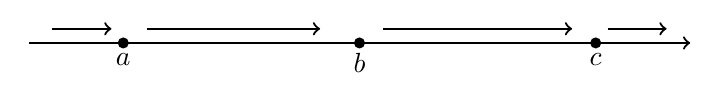
\begin{tikzpicture}[x=1cm,y=1cm,thick]
  \draw[->] (-4.2,0)--(4.2,0);
  \foreach \x/\lab in {-3/a,0/b,3/c} {\fill (\x,0) circle (2pt); \node[below] at (\x,0) {$\lab$};}
  \foreach \a/\b in {-2.7/-0.5,0.3/2.7} {\draw[->] (\a,0.18)--(\b,0.18);}
  \draw[->] (-3.9,0.18)--(-3.15,0.18); \draw[->] (3.15,0.18)--(3.9,0.18);
\end{tikzpicture}

 \caption{原书图 17：直线上各相邻平衡位置把相空间分成互不相交的区间；箭头表示当
 \(f>0\) 时轨线随 \(t\) 增大而向右运动，因此每个开区间都是一条单独的相轨线。}
 \label{fig:ch2-p2-17}
\end{figure}

证明先把 \(f(x_0)>0\) 局部化为 \(f>0\) 在 \((a,b)\) 上恒成立。只要 \(\varphi(t)\)
仍在 \((a,b)\) 中，它就只能从左向右运动；若在某个有限时刻越出右端点 \(b\)，就会与另一
条轨线 \(x=b\) 在有限时刻相遇，违反唯一性。左端同理。因此点不能在内部越界。

再证明极限达到相邻零点。假设
\(\lim_{t\to r_2}\varphi(t)=c\)，其中 \(c<b\)。取初值为 \(c\) 的另一条解。
因为 \(f(c)>0\)，该解在某个较早时刻会经过 \(c\) 的值，而 \(c\) 不属于原轨线的取值
范围，于是两条轨线相交，矛盾。因此只能有 \(\lim_{t\to r_2}\varphi(t)=b\)。左端
\(\lim_{t\to r_1}\varphi(t)=a\) 同理。最后，若 \(b<+\infty\) 而 \(r_2<+\infty\)，
把解在 \(r_2\) 之后接成常值 \(b\)，就会得到经过 \(b\) 的另一条解，也违反唯一性。
所以有限端点对应的存在时间必须是无穷。对左端点作同样论证。

现在设 \(b\) 是方程 \(x'=f(x)\) 的平衡位置，而 \((a,b)\) 与 \((b,c)\) 是左右相邻的
两个区间。如果当 \(t\) 增大时，两个相邻区间中的点都趋近于 \(b\)，就称 \(b\) 为稳定平衡
位置，见图~\ref{fig:ch2-p2-18}(a)。如果两边都离开 \(b\)，称它为不稳定的，见图
\ref{fig:ch2-p2-18}(b)。如果一边趋近而另一边离开，称它为半稳定的，见图
\ref{fig:ch2-p2-18}(c)。

\begin{figure}[H]
 \centering
 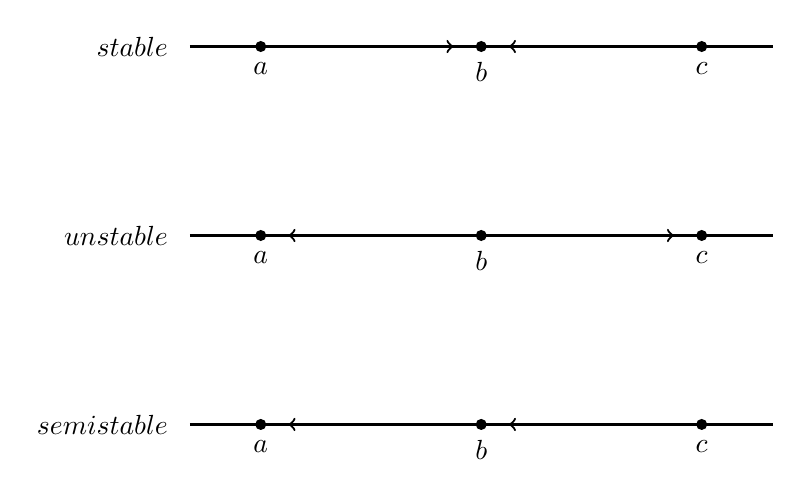
\begin{tikzpicture}[x=1cm,y=1cm,thick]
  % The three rows show the two intervals adjacent to b.
  \foreach \y/\case in {2.4/stable,0/unstable,-2.4/semistable} {
    \draw (-3.7,\y)--(3.7,\y);
    \foreach \x/\lab in {-2.8/a,0/b,2.8/c} {
      \fill (\x,\y) circle (2pt);
      \node[below=2pt] at (\x,\y) {$\lab$};
    }
    \node[left] at (-3.85,\y) {$\case$};
  }
  % Stable: both neighboring intervals flow toward b.
  \draw[->] (-2.45,2.4)--(-0.35,2.4);
  \draw[->] (2.45,2.4)--(0.35,2.4);
  % Unstable: both intervals flow away from b.
  \draw[<-] (-2.45,0)--(-0.35,0);
  \draw[->] (0.35,0)--(2.45,0);
  % Semistable: the left side leaves b while the right side approaches it.
  \draw[<-] (-2.45,-2.4)--(-0.35,-2.4);
  \draw[->] (2.45,-2.4)--(0.35,-2.4);
\end{tikzpicture}

 \caption{原书图 18：上、中、下三行分别表示稳定、不稳定和半稳定平衡位置。左右区间上
 的箭头由 \(f\) 的符号决定：指向 \(b\) 表示趋近，背离 \(b\) 表示离开；三个零点分别
 是 \(a,b,c\)。}
 \label{fig:ch2-p2-18}
\end{figure}

用函数符号判断，平衡位置 \(b\) 稳定，当且仅当 \(f\) 在 \((a,b)\) 上为正、在
\((b,c)\) 上为负；不稳定，当且仅当 \(f\) 在左侧为负、在右侧为正；半稳定，当且仅当
两侧同号。若 \(f'(b)\neq0\)，在 \(b\) 附近 \(f(x)\) 的符号与 \(f'(b)(x-b)\) 一致。
于是 \(f'(b)<0\) 时 \(b\) 稳定，\(f'(b)>0\) 时不稳定。若 \(f'(b)=0\)，一阶导数不能
给出结论，必须检查更高阶项或直接看左右符号。

\paragraph{例 2.}
考察方程
\begin{equation}
 x'=f(x),
 \tag{19}
\end{equation}
其中 \(f\) 是以 \(2\pi\) 为周期的连续可微函数：
\[
 f(x+2k\pi)=f(x),\qquad k\in\mathbb Z.
\]
例 1 的局部结论仍适用于每个标量解，但由于 \(f\) 的周期性，把相空间看成半径为 \(1\) 的
圆周 \(K\) 更合适。固定圆周上的计算起点 \(O\) 和逆时针方向；在圆周上取从 \(O\) 沿逆时针
方向弧长为 \(x\) 的点 \(\xi\)，再把所有实数 \(x\) 对应到 \(K\) 上的点。于是 \(x\) 与
\(x+2k\pi\) 对应同一个 \(\xi\)。因为 \(f\) 有相同周期，可以令
\[
 f(\xi)=f(x)
\]
把 \(f\) 看成定义在圆周 \(K\) 上的函数。

方程 \(x'=f(x)\) 于是描述了点在圆周上的运动。若 \(x(t)\) 是一个解，则对应的点
\(\xi(t)\) 沿圆周运动。若 \(\alpha\in K\) 满足 \(f(\alpha)=0\)，则 \(\xi=\alpha\)
是平衡位置。为简单起见，假设圆周上的平衡位置没有极限点，于是平衡位置只能有有限多个
或者一个也没有。平衡位置把圆周分成若干个区间；若没有平衡位置，整个圆周就是一个区间；
若恰有一个平衡位置 \(\alpha\)，则圆周去掉 \(\alpha\) 后也只有一个区间，其两个端点实际
上重合。

\begin{figure}[H]
 \centering
 \begin{tikzpicture}[x=1cm,y=1cm,thick,>=Stealth]
  \def\radius{1.8}
  % The full phase space is a circle; x is measured along its circumference.
  \draw[dashed] (0,0) circle (\radius);
  \draw[->,very thick]
    (\radius,0) arc[start angle=0,end angle=62,radius=\radius]
    node[midway,above right] {$x$};
  \fill (\radius,0) circle (2pt) node[right=3pt] {$O$};
  \fill ({\radius*cos(62)},{\radius*sin(62)}) circle (2pt)
    node[above right=2pt] {$\xi$};
  \node at (0,2.18) {$K$};
\end{tikzpicture}

 \caption{原书图 19：周期函数的相空间。圆周 \(K\) 上没有直角坐标轴，起点 \(O\)
 用来量弧长；实数 \(x\) 对应弧长 \(x\) 的点 \(\xi\)，\(x\) 与 \(x+2k\pi\) 落在
 同一点。参数条件是 \(f\) 以 \(2\pi\) 为周期。}
 \label{fig:ch2-p2-19}
\end{figure}

\begin{figure}[H]
 \centering
 \begin{tikzpicture}[scale=2.3542,font=\small,x=1cm,y=1cm,line width=0.8pt]
  % Six equilibria: three sinks alternate with three sources on the circle.
  \draw (0,0) circle (2);
  \foreach \ang in {0,76,132,213,256,286}
    \fill ({2*cos(\ang)},{2*sin(\ang)}) circle (1.6pt);
  \foreach \a/\b in {15/4,-15/-4,117/128,147/136,241/252,271/260}
    \draw[->] ({2*cos(\a)},{2*sin(\a)})
      arc[start angle=\a,end angle=\b,radius=2];
\end{tikzpicture}

 \caption{原书图 20：圆周 \(K\) 上的平衡点把圆周切成带方向的弧段。箭头显示各弧段内
 \(f\) 的符号所确定的运动方向；若没有平衡点，整圆是一条周期轨线，若只有一个平衡点，
 圆周去掉该点后仍是一条带有重合端点的轨线。}
 \label{fig:ch2-p2-20}
\end{figure}

取区间 \(I\) 中一点 \(\xi_0\)，设 \(x(t)\) 是以 \(x(0)=x_0\) 为初值的标量解，而
\(\xi(t)\) 是对应圆周上的点。若区间有端点，点沿确定方向运动，除端点外每一点都由轨线
经过一次。若区间就是整个圆周，则从位置 \(\xi_0\) 出发的点经过某段时间 \(T\) 回到
\(\xi_0\)，所以
\[
 \xi(0)=\xi(T).
\]
对应到原来的实变量 \(x(t)\)，有
\[
 x(t+T)=x(t)\pm2\pi,
\]
正负号由绕行方向决定。这个例子说明相空间不一定是欧氏坐标空间，可以是一个圆周；轨线的
几何形状必须与函数展开的周期性一起理解。

\paragraph{例 3.}
考虑平面周期系统
\begin{equation}
 x_i'=f_i(x_1,x_2),\qquad i=1,2,
 \tag{20}
\end{equation}
其中 \(f_i\) 连续可微，并有周期
\[
 f_i(x_1+2k\pi,x_2+2l\pi)=f_i(x_1,x_2),\qquad k,l\in\mathbb Z.
\]
此时把相空间看成环面最合适。在三维欧氏空间的 \((x,z)\) 平面中取圆心为 \((2,0,0)\)、
半径为 \(1\) 的圆 \(K\)。取点 \((3,0,0)\) 为计算起点。对每个 \(x_1\)，按例 2 的弧长
规则在 \(K\) 上取点 \(\xi_1\)。再绕 \(z\) 轴旋转 \((x,z)\) 平面，旋转角为 \(x_2\)；
圆 \(K\) 旋转所描出的曲面就是环面。若旋转角由 \(x_2\) 增加到 \(x_2+2\pi\)，平面回到
自身，环面上的点也回到同一点。因此环面上的一点由两个循环坐标 \((\xi_1,\xi_2)\)
完全确定，而每一对循环坐标唯一确定一点。

\begin{figure}[H]
 \centering
 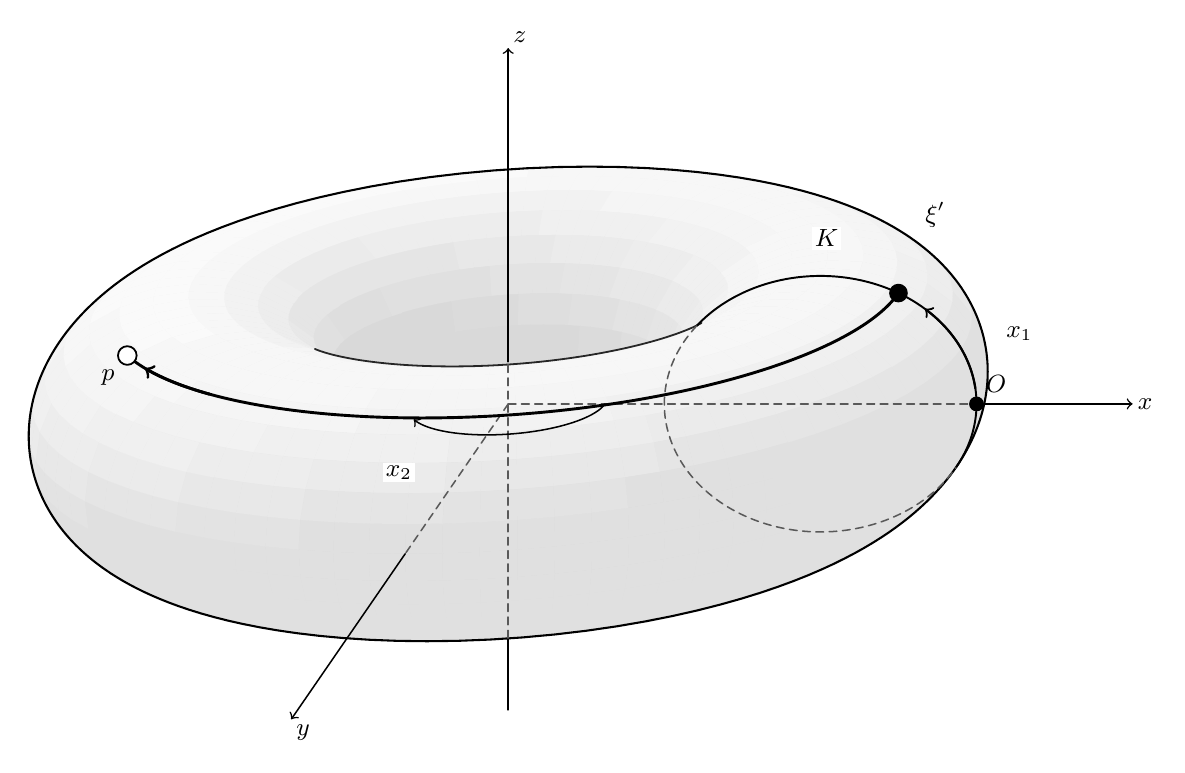
\begin{tikzpicture}[scale=1.9825,font=\small,x=1cm,y=1cm,line cap=round,line join=round,
  every node/.style={font=\small,inner sep=1.6pt},
  axis/.style={line width=.55pt},
  hidden/.style={line width=.55pt,dash pattern=on 2.8pt off 2pt,black!65}]
% Parametric torus ((2+cos v)cos u,(2+cos v)sin u,sin v).
% One consistent oblique projection: (X,Y)=(x-.22y,.82z-.32y).
% The small solid patches below are depth-sorted surface facets, not separate ellipses.
% They provide only a pale wash; the exact smooth contour is drawn afterwards.
  \path[fill=black!12,draw=black!12,line width=.10pt] (-0.0566,0.5469) -- (0.1765,0.5611) -- (0.1810,0.7578) -- (-0.0581,0.7432) -- cycle;
  \path[fill=black!12,draw=black!12,line width=.10pt] (-0.2895,0.5271) -- (-0.0566,0.5469) -- (-0.0581,0.7432) -- (-0.2969,0.7229) -- cycle;
  \path[fill=black!12,draw=black!12,line width=.10pt] (0.1765,0.5611) -- (0.4086,0.5697) -- (0.4191,0.7666) -- (0.1810,0.7578) -- cycle;
  \path[fill=black!12,draw=black!12,line width=.10pt] (-0.0543,0.3543) -- (0.1693,0.3680) -- (0.1765,0.5611) -- (-0.0566,0.5469) -- cycle;
  \path[fill=black!12,draw=black!12,line width=.10pt] (-0.2776,0.3354) -- (-0.0543,0.3543) -- (-0.0566,0.5469) -- (-0.2895,0.5271) -- cycle;
  \path[fill=black!12,draw=black!12,line width=.10pt] (-0.5205,0.5019) -- (-0.2895,0.5271) -- (-0.2969,0.7229) -- (-0.5338,0.6970) -- cycle;
  \path[fill=black!11,draw=black!11,line width=.10pt] (-0.0581,0.7432) -- (0.1810,0.7578) -- (0.1826,0.9482) -- (-0.0586,0.9335) -- cycle;
  \path[fill=black!12,draw=black!12,line width=.10pt] (0.1693,0.3680) -- (0.3919,0.3762) -- (0.4086,0.5697) -- (0.1765,0.5611) -- cycle;
  \path[fill=black!11,draw=black!11,line width=.10pt] (-0.2969,0.7229) -- (-0.0581,0.7432) -- (-0.0586,0.9335) -- (-0.2994,0.9130) -- cycle;
  \path[fill=black!12,draw=black!12,line width=.10pt] (0.4086,0.5697) -- (0.6382,0.5725) -- (0.6545,0.7695) -- (0.4191,0.7666) -- cycle;
  \path[fill=black!12,draw=black!12,line width=.10pt] (-0.4991,0.3112) -- (-0.2776,0.3354) -- (-0.2895,0.5271) -- (-0.5205,0.5019) -- cycle;
  \path[fill=black!11,draw=black!11,line width=.10pt] (0.1810,0.7578) -- (0.4191,0.7666) -- (0.4226,0.9570) -- (0.1826,0.9482) -- cycle;
  \path[fill=black!11,draw=black!11,line width=.10pt] (-0.5338,0.6970) -- (-0.2969,0.7229) -- (-0.2994,0.9130) -- (-0.5383,0.8869) -- cycle;
  \path[fill=black!12,draw=black!12,line width=.10pt] (0.3919,0.3762) -- (0.6120,0.3789) -- (0.6382,0.5725) -- (0.4086,0.5697) -- cycle;
  \path[fill=black!12,draw=black!12,line width=.10pt] (-0.7484,0.4713) -- (-0.5205,0.5019) -- (-0.5338,0.6970) -- (-0.7674,0.6658) -- cycle;
  \path[fill=black!12,draw=black!12,line width=.10pt] (0.4191,0.7666) -- (0.6545,0.7695) -- (0.6600,0.9600) -- (0.4226,0.9570) -- cycle;
  \path[fill=black!12,draw=black!12,line width=.10pt] (-0.7176,0.2819) -- (-0.4991,0.3112) -- (-0.5205,0.5019) -- (-0.7484,0.4713) -- cycle;
  \path[fill=black!12,draw=black!12,line width=.10pt] (-0.0512,0.1752) -- (0.1597,0.1881) -- (0.1693,0.3680) -- (-0.0543,0.3543) -- cycle;
  \path[fill=black!12,draw=black!12,line width=.10pt] (0.6382,0.5725) -- (0.8639,0.5697) -- (0.8859,0.7666) -- (0.6545,0.7695) -- cycle;
  \path[fill=black!12,draw=black!12,line width=.10pt] (-0.2618,0.1573) -- (-0.0512,0.1752) -- (-0.0543,0.3543) -- (-0.2776,0.3354) -- cycle;
  \path[fill=black!10,draw=black!10,line width=.10pt] (-0.7674,0.6658) -- (-0.5338,0.6970) -- (-0.5383,0.8869) -- (-0.7739,0.8554) -- cycle;
  \path[fill=black!12,draw=black!12,line width=.10pt] (0.1597,0.1881) -- (0.3696,0.1958) -- (0.3919,0.3762) -- (0.1693,0.3680) -- cycle;
  \path[fill=black!12,draw=black!12,line width=.10pt] (0.6120,0.3789) -- (0.8284,0.3762) -- (0.8639,0.5697) -- (0.6382,0.5725) -- cycle;
  \path[fill=black!12,draw=black!12,line width=.10pt] (-0.4707,0.1345) -- (-0.2618,0.1573) -- (-0.2776,0.3354) -- (-0.4991,0.3112) -- cycle;
  \path[fill=black!9,draw=black!9,line width=.10pt] (-0.0586,0.9335) -- (0.1826,0.9482) -- (0.1810,1.1227) -- (-0.0581,1.1081) -- cycle;
  \path[fill=black!9,draw=black!9,line width=.10pt] (-0.2994,0.9130) -- (-0.0586,0.9335) -- (-0.0581,1.1081) -- (-0.2969,1.0879) -- cycle;
  \path[fill=black!12,draw=black!12,line width=.10pt] (-0.9716,0.4357) -- (-0.7484,0.4713) -- (-0.7674,0.6658) -- (-0.9964,0.6292) -- cycle;
  \path[fill=black!12,draw=black!12,line width=.10pt] (0.6545,0.7695) -- (0.8859,0.7666) -- (0.8933,0.9570) -- (0.6600,0.9600) -- cycle;
  \path[fill=black!9,draw=black!9,line width=.10pt] (0.1826,0.9482) -- (0.4226,0.9570) -- (0.4191,1.1315) -- (0.1810,1.1227) -- cycle;
  \path[fill=black!12,draw=black!12,line width=.10pt] (0.3696,0.1958) -- (0.5772,0.1984) -- (0.6120,0.3789) -- (0.3919,0.3762) -- cycle;
  \path[fill=black!12,draw=black!12,line width=.10pt] (-0.9317,0.2477) -- (-0.7176,0.2819) -- (-0.7484,0.4713) -- (-0.9716,0.4357) -- cycle;
  \path[fill=black!9,draw=black!9,line width=.10pt] (-0.5383,0.8869) -- (-0.2994,0.9130) -- (-0.2969,1.0879) -- (-0.5338,1.0620) -- cycle;
  \path[fill=black!12,draw=black!12,line width=.10pt] (-0.6768,0.1069) -- (-0.4707,0.1345) -- (-0.4991,0.3112) -- (-0.7176,0.2819) -- cycle;
  \path[fill=black!10,draw=black!10,line width=.10pt] (-0.9964,0.6292) -- (-0.7674,0.6658) -- (-0.7739,0.8554) -- (-1.0048,0.8185) -- cycle;
  \path[fill=black!12,draw=black!12,line width=.10pt] (0.8639,0.5697) -- (1.0842,0.5611) -- (1.1118,0.7578) -- (0.8859,0.7666) -- cycle;
  \path[fill=black!9,draw=black!9,line width=.10pt] (0.4226,0.9570) -- (0.6600,0.9600) -- (0.6545,1.1344) -- (0.4191,1.1315) -- cycle;
  \path[fill=black!12,draw=black!12,line width=.10pt] (0.8284,0.3762) -- (1.0396,0.3680) -- (1.0842,0.5611) -- (0.8639,0.5697) -- cycle;
  \path[fill=black!12,draw=black!12,line width=.10pt] (0.5772,0.1984) -- (0.7812,0.1958) -- (0.8284,0.3762) -- (0.6120,0.3789) -- cycle;
  \path[fill=black!8,draw=black!8,line width=.10pt] (-0.7739,0.8554) -- (-0.5383,0.8869) -- (-0.5338,1.0620) -- (-0.7674,1.0307) -- cycle;
  \path[fill=black!12,draw=black!12,line width=.10pt] (0.8859,0.7666) -- (1.1118,0.7578) -- (1.1212,0.9482) -- (0.8933,0.9570) -- cycle;
  \path[fill=black!12,draw=black!12,line width=.10pt] (-1.1888,0.3952) -- (-0.9716,0.4357) -- (-0.9964,0.6292) -- (-1.2191,0.5877) -- cycle;
  \path[fill=black!12,draw=black!12,line width=.10pt] (-0.8787,0.0747) -- (-0.6768,0.1069) -- (-0.7176,0.2819) -- (-0.9317,0.2477) -- cycle;
  \path[fill=black!12,draw=black!12,line width=.10pt] (-1.1400,0.2089) -- (-0.9317,0.2477) -- (-0.9716,0.4357) -- (-1.1888,0.3952) -- cycle;
  \path[fill=black!12,draw=black!12,line width=.10pt] (-0.0475,0.0185) -- (0.1481,0.0305) -- (0.1597,0.1881) -- (-0.0512,0.1752) -- cycle;
  \path[fill=black!10,draw=black!10,line width=.10pt] (0.6600,0.9600) -- (0.8933,0.9570) -- (0.8859,1.1315) -- (0.6545,1.1344) -- cycle;
  \path[fill=black!12,draw=black!12,line width=.10pt] (-0.2429,0.0019) -- (-0.0475,0.0185) -- (-0.0512,0.1752) -- (-0.2618,0.1573) -- cycle;
  \path[fill=black!12,draw=black!12,line width=.10pt] (0.1481,0.0305) -- (0.3428,0.0376) -- (0.3696,0.1958) -- (0.1597,0.1881) -- cycle;
  \path[fill=black!10,draw=black!10,line width=.10pt] (-1.2191,0.5877) -- (-0.9964,0.6292) -- (-1.0048,0.8185) -- (-1.2294,0.7767) -- cycle;
  \path[fill=black!12,draw=black!12,line width=.10pt] (-0.4367,-0.0192) -- (-0.2429,0.0019) -- (-0.2618,0.1573) -- (-0.4707,0.1345) -- cycle;
  \path[fill=black!12,draw=black!12,line width=.10pt] (0.7812,0.1958) -- (0.9805,0.1881) -- (1.0396,0.3680) -- (0.8284,0.3762) -- cycle;
  \path[fill=black!8,draw=black!8,line width=.10pt] (-1.0048,0.8185) -- (-0.7739,0.8554) -- (-0.7674,1.0307) -- (-0.9964,0.9942) -- cycle;
  \path[fill=black!12,draw=black!12,line width=.10pt] (1.0842,0.5611) -- (1.2978,0.5469) -- (1.3309,0.7432) -- (1.1118,0.7578) -- cycle;
  \path[fill=black!7,draw=black!7,line width=.10pt] (-0.0581,1.1081) -- (0.1810,1.1227) -- (0.1765,1.2727) -- (-0.0566,1.2584) -- cycle;
  \path[fill=black!12,draw=black!12,line width=.10pt] (0.3428,0.0376) -- (0.5355,0.0400) -- (0.5772,0.1984) -- (0.3696,0.1958) -- cycle;
  \path[fill=black!7,draw=black!7,line width=.10pt] (-0.2969,1.0879) -- (-0.0581,1.1081) -- (-0.0566,1.2584) -- (-0.2895,1.2387) -- cycle;
  \path[fill=black!12,draw=black!12,line width=.10pt] (1.0396,0.3680) -- (1.2445,0.3543) -- (1.2978,0.5469) -- (1.0842,0.5611) -- cycle;
  \path[fill=black!7,draw=black!7,line width=.10pt] (0.1810,1.1227) -- (0.4191,1.1315) -- (0.4086,1.2812) -- (0.1765,1.2727) -- cycle;
  \path[fill=black!12,draw=black!12,line width=.10pt] (-0.6279,-0.0448) -- (-0.4367,-0.0192) -- (-0.4707,0.1345) -- (-0.6768,0.1069) -- cycle;
  \path[fill=black!12,draw=black!12,line width=.10pt] (-1.0751,0.0381) -- (-0.8787,0.0747) -- (-0.9317,0.2477) -- (-1.1400,0.2089) -- cycle;
  \path[fill=black!7,draw=black!7,line width=.10pt] (-0.5338,1.0620) -- (-0.2969,1.0879) -- (-0.2895,1.2387) -- (-0.5205,1.2134) -- cycle;
  \path[fill=black!10,draw=black!10,line width=.10pt] (0.8933,0.9570) -- (1.1212,0.9482) -- (1.1118,1.1227) -- (0.8859,1.1315) -- cycle;
  \path[fill=black!12,draw=black!12,line width=.10pt] (1.1118,0.7578) -- (1.3309,0.7432) -- (1.3421,0.9335) -- (1.1212,0.9482) -- cycle;
  \path[fill=black!12,draw=black!12,line width=.10pt] (-1.3987,0.3501) -- (-1.1888,0.3952) -- (-1.2191,0.5877) -- (-1.4344,0.5414) -- cycle;
  \path[fill=black!12,draw=black!12,line width=.10pt] (0.5355,0.0400) -- (0.7248,0.0376) -- (0.7812,0.1958) -- (0.5772,0.1984) -- cycle;
  \path[fill=black!7,draw=black!7,line width=.10pt] (0.4191,1.1315) -- (0.6545,1.1344) -- (0.6382,1.2841) -- (0.4086,1.2812) -- cycle;
  \path[fill=black!12,draw=black!12,line width=.10pt] (-1.3413,0.1656) -- (-1.1400,0.2089) -- (-1.1888,0.3952) -- (-1.3987,0.3501) -- cycle;
  \path[fill=black!6,draw=black!6,line width=.10pt] (-0.7674,1.0307) -- (-0.5338,1.0620) -- (-0.5205,1.2134) -- (-0.7484,1.1829) -- cycle;
  \path[fill=black!12,draw=black!12,line width=.10pt] (0.9805,0.1881) -- (1.1737,0.1752) -- (1.2445,0.3543) -- (1.0396,0.3680) -- cycle;
  \path[fill=black!12,draw=black!12,line width=.10pt] (-0.8152,-0.0747) -- (-0.6279,-0.0448) -- (-0.6768,0.1069) -- (-0.8787,0.0747) -- cycle;
  \path[fill=black!8,draw=black!8,line width=.10pt] (-1.2294,0.7767) -- (-1.0048,0.8185) -- (-0.9964,0.9942) -- (-1.2191,0.9526) -- cycle;
  \path[fill=black!10,draw=black!10,line width=.10pt] (-1.4344,0.5414) -- (-1.2191,0.5877) -- (-1.2294,0.7767) -- (-1.4465,0.7300) -- cycle;
  \path[fill=black!8,draw=black!8,line width=.10pt] (0.6545,1.1344) -- (0.8859,1.1315) -- (0.8639,1.2812) -- (0.6382,1.2841) -- cycle;
  \path[fill=black!12,draw=black!12,line width=.10pt] (1.2978,0.5469) -- (1.5034,0.5271) -- (1.5418,0.7229) -- (1.3309,0.7432) -- cycle;
  \path[fill=black!12,draw=black!12,line width=.10pt] (0.7248,0.0376) -- (0.9096,0.0305) -- (0.9805,0.1881) -- (0.7812,0.1958) -- cycle;
  \path[fill=black!12,draw=black!12,line width=.10pt] (1.2445,0.3543) -- (1.4417,0.3354) -- (1.5034,0.5271) -- (1.2978,0.5469) -- cycle;
  \path[fill=black!12,draw=black!12,line width=.10pt] (-1.2649,-0.0027) -- (-1.0751,0.0381) -- (-1.1400,0.2089) -- (-1.3413,0.1656) -- cycle;
  \path[fill=black!10,draw=black!10,line width=.10pt] (1.1212,0.9482) -- (1.3421,0.9335) -- (1.3309,1.1081) -- (1.1118,1.1227) -- cycle;
  \path[fill=black!6,draw=black!6,line width=.10pt] (-0.9964,0.9942) -- (-0.7674,1.0307) -- (-0.7484,1.1829) -- (-0.9716,1.1473) -- cycle;
  \path[fill=black!12,draw=black!12,line width=.10pt] (-0.0434,-0.1079) -- (0.1353,-0.0970) -- (0.1481,0.0305) -- (-0.0475,0.0185) -- cycle;
  \path[fill=black!12,draw=black!12,line width=.10pt] (-0.2218,-0.1230) -- (-0.0434,-0.1079) -- (-0.0475,0.0185) -- (-0.2429,0.0019) -- cycle;
  \path[fill=black!12,draw=black!12,line width=.10pt] (1.3309,0.7432) -- (1.5418,0.7229) -- (1.5547,0.9130) -- (1.3421,0.9335) -- cycle;
  \path[fill=black!12,draw=black!12,line width=.10pt] (-0.9974,-0.1087) -- (-0.8152,-0.0747) -- (-0.8787,0.0747) -- (-1.0751,0.0381) -- cycle;
  \path[fill=black!12,draw=black!12,line width=.10pt] (0.1353,-0.0970) -- (0.3131,-0.0904) -- (0.3428,0.0376) -- (0.1481,0.0305) -- cycle;
  \path[fill=black!12,draw=black!12,line width=.10pt] (-0.3988,-0.1424) -- (-0.2218,-0.1230) -- (-0.2429,0.0019) -- (-0.4367,-0.0192) -- cycle;
  \path[fill=black!12,draw=black!12,line width=.10pt] (-1.6000,0.3006) -- (-1.3987,0.3501) -- (-1.4344,0.5414) -- (-1.6408,0.4907) -- cycle;
  \path[fill=black!12,draw=black!12,line width=.10pt] (-1.5343,0.1182) -- (-1.3413,0.1656) -- (-1.3987,0.3501) -- (-1.6000,0.3006) -- cycle;
  \path[fill=black!12,draw=black!12,line width=.10pt] (1.1737,0.1752) -- (1.3596,0.1573) -- (1.4417,0.3354) -- (1.2445,0.3543) -- cycle;
  \path[fill=black!8,draw=black!8,line width=.10pt] (0.8859,1.1315) -- (1.1118,1.1227) -- (1.0842,1.2727) -- (0.8639,1.2812) -- cycle;
  \path[fill=black!12,draw=black!12,line width=.10pt] (0.3131,-0.0904) -- (0.4890,-0.0882) -- (0.5355,0.0400) -- (0.3428,0.0376) -- cycle;
  \path[fill=black!8,draw=black!8,line width=.10pt] (-1.4465,0.7300) -- (-1.2294,0.7767) -- (-1.2191,0.9526) -- (-1.4344,0.9064) -- cycle;
  \path[fill=black!5,draw=black!5,line width=.10pt] (-0.0566,1.2584) -- (0.1765,1.2727) -- (0.1693,1.3905) -- (-0.0543,1.3769) -- cycle;
  \path[fill=black!12,draw=black!12,line width=.10pt] (0.9096,0.0305) -- (1.0888,0.0185) -- (1.1737,0.1752) -- (0.9805,0.1881) -- cycle;
  \path[fill=black!5,draw=black!5,line width=.10pt] (-0.2895,1.2387) -- (-0.0566,1.2584) -- (-0.0543,1.3769) -- (-0.2776,1.3579) -- cycle;
  \path[fill=black!12,draw=black!12,line width=.10pt] (-0.5733,-0.1658) -- (-0.3988,-0.1424) -- (-0.4367,-0.0192) -- (-0.6279,-0.0448) -- cycle;
  \path[fill=black!6,draw=black!6,line width=.10pt] (0.1765,1.2727) -- (0.4086,1.2812) -- (0.3919,1.3987) -- (0.1693,1.3905) -- cycle;
  \path[fill=black!10,draw=black!10,line width=.10pt] (-1.6408,0.4907) -- (-1.4344,0.5414) -- (-1.4465,0.7300) -- (-1.6546,0.6788) -- cycle;
  \path[fill=black!5,draw=black!5,line width=.10pt] (-0.5205,1.2134) -- (-0.2895,1.2387) -- (-0.2776,1.3579) -- (-0.4991,1.3337) -- cycle;
  \path[fill=black!6,draw=black!6,line width=.10pt] (-1.2191,0.9526) -- (-0.9964,0.9942) -- (-0.9716,1.1473) -- (-1.1888,1.1068) -- cycle;
  \path[fill=black!12,draw=black!12,line width=.10pt] (0.4890,-0.0882) -- (0.6618,-0.0904) -- (0.7248,0.0376) -- (0.5355,0.0400) -- cycle;
  \path[fill=black!12,draw=black!12,line width=.10pt] (-1.4470,-0.0475) -- (-1.2649,-0.0027) -- (-1.3413,0.1656) -- (-1.5343,0.1182) -- cycle;
  \path[fill=black!12,draw=black!12,line width=.10pt] (1.5034,0.5271) -- (1.6998,0.5019) -- (1.7431,0.6970) -- (1.5418,0.7229) -- cycle;
  \path[fill=black!12,draw=black!12,line width=.10pt] (-1.1735,-0.1466) -- (-0.9974,-0.1087) -- (-1.0751,0.0381) -- (-1.2649,-0.0027) -- cycle;
  \path[fill=black!12,draw=black!12,line width=.10pt] (1.4417,0.3354) -- (1.6300,0.3112) -- (1.6998,0.5019) -- (1.5034,0.5271) -- cycle;
  \path[fill=black!6,draw=black!6,line width=.10pt] (0.4086,1.2812) -- (0.6382,1.2841) -- (0.6120,1.4014) -- (0.3919,1.3987) -- cycle;
  \path[fill=black!10,draw=black!10,line width=.10pt] (1.3421,0.9335) -- (1.5547,0.9130) -- (1.5418,1.0879) -- (1.3309,1.1081) -- cycle;
  \path[fill=black!12,draw=black!12,line width=.10pt] (-0.7444,-0.1930) -- (-0.5733,-0.1658) -- (-0.6279,-0.0448) -- (-0.8152,-0.0747) -- cycle;
  \path[fill=black!5,draw=black!5,line width=.10pt] (-0.7484,1.1829) -- (-0.5205,1.2134) -- (-0.4991,1.3337) -- (-0.7176,1.3044) -- cycle;
  \path[fill=black!8,draw=black!8,line width=.10pt] (1.1118,1.1227) -- (1.3309,1.1081) -- (1.2978,1.2584) -- (1.0842,1.2727) -- cycle;
  \path[fill=black!12,draw=black!12,line width=.10pt] (1.5418,0.7229) -- (1.7431,0.6970) -- (1.7578,0.8869) -- (1.5547,0.9130) -- cycle;
  \path[fill=black!12,draw=black!12,line width=.10pt] (0.6618,-0.0904) -- (0.8306,-0.0970) -- (0.9096,0.0305) -- (0.7248,0.0376) -- cycle;
  \path[fill=black!12,draw=black!12,line width=.10pt] (1.0888,0.0185) -- (1.2614,0.0019) -- (1.3596,0.1573) -- (1.1737,0.1752) -- cycle;
  \path[fill=black!6,draw=black!6,line width=.10pt] (0.6382,1.2841) -- (0.8639,1.2812) -- (0.8284,1.3987) -- (0.6120,1.4014) -- cycle;
  \path[fill=black!12,draw=black!12,line width=.10pt] (1.3596,0.1573) -- (1.5372,0.1345) -- (1.6300,0.3112) -- (1.4417,0.3354) -- cycle;
  \path[fill=black!12,draw=black!12,line width=.10pt] (-1.7914,0.2471) -- (-1.6000,0.3006) -- (-1.6408,0.4907) -- (-1.8371,0.4358) -- cycle;
  \path[fill=black!8,draw=black!8,line width=.10pt] (-1.6546,0.6788) -- (-1.4465,0.7300) -- (-1.4344,0.9064) -- (-1.6408,0.8556) -- cycle;
  \path[fill=black!12,draw=black!12,line width=.10pt] (-1.7179,0.0669) -- (-1.5343,0.1182) -- (-1.6000,0.3006) -- (-1.7914,0.2471) -- cycle;
  \path[fill=black!12,draw=black!12,line width=.10pt] (-0.9108,-0.2241) -- (-0.7444,-0.1930) -- (-0.8152,-0.0747) -- (-0.9974,-0.1087) -- cycle;
  \path[fill=black!6,draw=black!6,line width=.10pt] (-1.4344,0.9064) -- (-1.2191,0.9526) -- (-1.1888,1.1068) -- (-1.3987,1.0617) -- cycle;
  \path[fill=black!5,draw=black!5,line width=.10pt] (-0.9716,1.1473) -- (-0.7484,1.1829) -- (-0.7176,1.3044) -- (-0.9317,1.2703) -- cycle;
  \path[fill=black!12,draw=black!12,line width=.10pt] (-1.3424,-0.1881) -- (-1.1735,-0.1466) -- (-1.2649,-0.0027) -- (-1.4470,-0.0475) -- cycle;
  \path[fill=black!10,draw=black!10,line width=.10pt] (-1.8371,0.4358) -- (-1.6408,0.4907) -- (-1.6546,0.6788) -- (-1.8526,0.6235) -- cycle;
  \path[fill=black!12,draw=black!12,line width=.10pt] (0.8306,-0.0970) -- (0.9943,-0.1079) -- (1.0888,0.0185) -- (0.9096,0.0305) -- cycle;
  \path[fill=black!12,draw=black!12,line width=.10pt] (-1.6201,-0.0959) -- (-1.4470,-0.0475) -- (-1.5343,0.1182) -- (-1.7179,0.0669) -- cycle;
  \path[fill=black!12,draw=black!12,line width=.10pt] (-0.0390,-0.1977) -- (0.1217,-0.1879) -- (0.1353,-0.0970) -- (-0.0434,-0.1079) -- cycle;
  \path[fill=black!12,draw=black!12,line width=.10pt] (-0.1996,-0.2113) -- (-0.0390,-0.1977) -- (-0.0434,-0.1079) -- (-0.2218,-0.1230) -- cycle;
  \path[fill=black!6,draw=black!6,line width=.10pt] (0.8639,1.2812) -- (1.0842,1.2727) -- (1.0396,1.3905) -- (0.8284,1.3987) -- cycle;
  \path[fill=black!12,draw=black!12,line width=.10pt] (0.1217,-0.1879) -- (0.2817,-0.1820) -- (0.3131,-0.0904) -- (0.1353,-0.0970) -- cycle;
  \path[fill=black!11,draw=black!11,line width=.10pt] (1.5547,0.9130) -- (1.7578,0.8869) -- (1.7431,1.0620) -- (1.5418,1.0879) -- cycle;
  \path[fill=black!12,draw=black!12,line width=.10pt] (1.6998,0.5019) -- (1.8857,0.4713) -- (1.9337,0.6658) -- (1.7431,0.6970) -- cycle;
  \path[fill=black!12,draw=black!12,line width=.10pt] (1.6300,0.3112) -- (1.8082,0.2819) -- (1.8857,0.4713) -- (1.6998,0.5019) -- cycle;
  \path[fill=black!12,draw=black!12,line width=.10pt] (-0.3589,-0.2287) -- (-0.1996,-0.2113) -- (-0.2218,-0.1230) -- (-0.3988,-0.1424) -- cycle;
  \path[fill=black!8,draw=black!8,line width=.10pt] (1.3309,1.1081) -- (1.5418,1.0879) -- (1.5034,1.2387) -- (1.2978,1.2584) -- cycle;
  \path[fill=black!12,draw=black!12,line width=.10pt] (0.2817,-0.1820) -- (0.4400,-0.1800) -- (0.4890,-0.0882) -- (0.3131,-0.0904) -- cycle;
  \path[fill=black!12,draw=black!12,line width=.10pt] (-1.0716,-0.2586) -- (-0.9108,-0.2241) -- (-0.9974,-0.1087) -- (-1.1735,-0.1466) -- cycle;
  \path[fill=black!12,draw=black!12,line width=.10pt] (1.2614,0.0019) -- (1.4261,-0.0192) -- (1.5372,0.1345) -- (1.3596,0.1573) -- cycle;
  \path[fill=black!5,draw=black!5,line width=.10pt] (-1.1888,1.1068) -- (-0.9716,1.1473) -- (-0.9317,1.2703) -- (-1.1400,1.2314) -- cycle;
  \path[fill=black!12,draw=black!12,line width=.10pt] (-0.5159,-0.2498) -- (-0.3589,-0.2287) -- (-0.3988,-0.1424) -- (-0.5733,-0.1658) -- cycle;
  \path[fill=black!4,draw=black!4,line width=.10pt] (-0.0543,1.3769) -- (0.1693,1.3905) -- (0.1597,1.4703) -- (-0.0512,1.4574) -- cycle;
  \path[fill=black!4,draw=black!4,line width=.10pt] (-0.2776,1.3579) -- (-0.0543,1.3769) -- (-0.0512,1.4574) -- (-0.2618,1.4395) -- cycle;
  \path[fill=black!12,draw=black!12,line width=.10pt] (1.7431,0.6970) -- (1.9337,0.6658) -- (1.9500,0.8554) -- (1.7578,0.8869) -- cycle;
  \path[fill=black!12,draw=black!12,line width=.10pt] (1.5372,0.1345) -- (1.7053,0.1069) -- (1.8082,0.2819) -- (1.6300,0.3112) -- cycle;
  \path[fill=black!4,draw=black!4,line width=.10pt] (0.1693,1.3905) -- (0.3919,1.3987) -- (0.3696,1.4780) -- (0.1597,1.4703) -- cycle;
  \path[fill=black!12,draw=black!12,line width=.10pt] (0.4400,-0.1800) -- (0.5956,-0.1820) -- (0.6618,-0.0904) -- (0.4890,-0.0882) -- cycle;
  \path[fill=black!6,draw=black!6,line width=.10pt] (-1.6408,0.8556) -- (-1.4344,0.9064) -- (-1.3987,1.0617) -- (-1.6000,1.0122) -- cycle;
  \path[fill=black!8,draw=black!8,line width=.10pt] (-1.8526,0.6235) -- (-1.6546,0.6788) -- (-1.6408,0.8556) -- (-1.8371,0.8007) -- cycle;
  \path[fill=black!12,draw=black!12,line width=.10pt] (0.9943,-0.1079) -- (1.1518,-0.1230) -- (1.2614,0.0019) -- (1.0888,0.0185) -- cycle;
  \path[fill=black!4,draw=black!4,line width=.10pt] (-0.4991,1.3337) -- (-0.2776,1.3579) -- (-0.2618,1.4395) -- (-0.4707,1.4167) -- cycle;
  \path[fill=black!6,draw=black!6,line width=.10pt] (1.0842,1.2727) -- (1.2978,1.2584) -- (1.2445,1.3769) -- (1.0396,1.3905) -- cycle;
  \path[fill=black!12,draw=black!12,line width=.10pt] (-1.8908,0.0120) -- (-1.7179,0.0669) -- (-1.7914,0.2471) -- (-1.9718,0.1899) -- cycle;
  \path[fill=black!12,draw=black!12,line width=.10pt] (-1.9718,0.1899) -- (-1.7914,0.2471) -- (-1.8371,0.4358) -- (-2.0221,0.3771) -- cycle;
  \path[fill=black!12,draw=black!12,line width=.10pt] (-1.5030,-0.2330) -- (-1.3424,-0.1881) -- (-1.4470,-0.0475) -- (-1.6201,-0.0959) -- cycle;
  \path[fill=black!12,draw=black!12,line width=.10pt] (-0.6698,-0.2743) -- (-0.5159,-0.2498) -- (-0.5733,-0.1658) -- (-0.7444,-0.1930) -- cycle;
  \path[fill=black!4,draw=black!4,line width=.10pt] (0.3919,1.3987) -- (0.6120,1.4014) -- (0.5772,1.4806) -- (0.3696,1.4780) -- cycle;
  \path[fill=black!4,draw=black!4,line width=.10pt] (-0.7176,1.3044) -- (-0.4991,1.3337) -- (-0.4707,1.4167) -- (-0.6768,1.3891) -- cycle;
  \path[fill=black!12,draw=black!12,line width=.10pt] (0.5956,-0.1820) -- (0.7475,-0.1879) -- (0.8306,-0.0970) -- (0.6618,-0.0904) -- cycle;
  \path[fill=black!12,draw=black!12,line width=.10pt] (-1.2258,-0.2965) -- (-1.0716,-0.2586) -- (-1.1735,-0.1466) -- (-1.3424,-0.1881) -- cycle;
  \path[fill=black!12,draw=black!12,line width=.10pt] (-1.7832,-0.1476) -- (-1.6201,-0.0959) -- (-1.7179,0.0669) -- (-1.8908,0.0120) -- cycle;
  \path[fill=black!4,draw=black!4,line width=.10pt] (-1.3987,1.0617) -- (-1.1888,1.1068) -- (-1.1400,1.2314) -- (-1.3413,1.1882) -- cycle;
  \path[fill=black!10,draw=black!10,line width=.10pt] (-2.0221,0.3771) -- (-1.8371,0.4358) -- (-1.8526,0.6235) -- (-2.0391,0.5643) -- cycle;
  \path[fill=black!9,draw=black!9,line width=.10pt] (1.5418,1.0879) -- (1.7431,1.0620) -- (1.6998,1.2134) -- (1.5034,1.2387) -- cycle;
  \path[fill=black!4,draw=black!4,line width=.10pt] (0.6120,1.4014) -- (0.8284,1.3987) -- (0.7812,1.4780) -- (0.5772,1.4806) -- cycle;
  \path[fill=black!12,draw=black!12,line width=.10pt] (-0.8196,-0.3022) -- (-0.6698,-0.2743) -- (-0.7444,-0.1930) -- (-0.9108,-0.2241) -- cycle;
  \path[fill=black!11,draw=black!11,line width=.10pt] (1.7578,0.8869) -- (1.9500,0.8554) -- (1.9337,1.0307) -- (1.7431,1.0620) -- cycle;
  \path[fill=black!12,draw=black!12,line width=.10pt] (1.4261,-0.0192) -- (1.5821,-0.0448) -- (1.7053,0.1069) -- (1.5372,0.1345) -- cycle;
  \path[fill=black!12,draw=black!12,line width=.10pt] (1.8082,0.2819) -- (1.9753,0.2477) -- (2.0599,0.4357) -- (1.8857,0.4713) -- cycle;
  \path[fill=black!12,draw=black!12,line width=.10pt] (1.8857,0.4713) -- (2.0599,0.4357) -- (2.1124,0.6292) -- (1.9337,0.6658) -- cycle;
  \path[fill=black!12,draw=black!12,line width=.10pt] (1.1518,-0.1230) -- (1.3023,-0.1424) -- (1.4261,-0.0192) -- (1.2614,0.0019) -- cycle;
  \path[fill=black!3,draw=black!3,line width=.10pt] (-0.9317,1.2703) -- (-0.7176,1.3044) -- (-0.6768,1.3891) -- (-0.8787,1.3569) -- cycle;
  \path[fill=black!12,draw=black!12,line width=.10pt] (0.7475,-0.1879) -- (0.8947,-0.1977) -- (0.9943,-0.1079) -- (0.8306,-0.0970) -- cycle;
  \path[fill=black!7,draw=black!7,line width=.10pt] (1.2978,1.2584) -- (1.5034,1.2387) -- (1.4417,1.3579) -- (1.2445,1.3769) -- cycle;
  \path[fill=black!12,draw=black!12,line width=.10pt] (1.7053,0.1069) -- (1.8629,0.0747) -- (1.9753,0.2477) -- (1.8082,0.2819) -- cycle;
  \path[fill=black!6,draw=black!6,line width=.10pt] (-1.8371,0.8007) -- (-1.6408,0.8556) -- (-1.6000,1.0122) -- (-1.7914,0.9587) -- cycle;
  \path[fill=black!5,draw=black!5,line width=.10pt] (0.8284,1.3987) -- (1.0396,1.3905) -- (0.9805,1.4703) -- (0.7812,1.4780) -- cycle;
  \path[fill=black!12,draw=black!12,line width=.10pt] (-1.6543,-0.2810) -- (-1.5030,-0.2330) -- (-1.6201,-0.0959) -- (-1.7832,-0.1476) -- cycle;
  \path[fill=black!12,draw=black!12,line width=.10pt] (-0.9643,-0.3333) -- (-0.8196,-0.3022) -- (-0.9108,-0.2241) -- (-1.0716,-0.2586) -- cycle;
  \path[fill=black!12,draw=black!12,line width=.10pt] (1.9337,0.6658) -- (2.1124,0.6292) -- (2.1302,0.8185) -- (1.9500,0.8554) -- cycle;
  \path[fill=black!8,draw=black!8,line width=.10pt] (-2.0391,0.5643) -- (-1.8526,0.6235) -- (-1.8371,0.8007) -- (-2.0221,0.7420) -- cycle;
  \path[fill=black!12,draw=black!12,line width=.10pt] (-1.3725,-0.3375) -- (-1.2258,-0.2965) -- (-1.3424,-0.1881) -- (-1.5030,-0.2330) -- cycle;
  \path[fill=black!12,draw=black!12,line width=.10pt] (-0.0347,-0.2464) -- (0.1082,-0.2377) -- (0.1217,-0.1879) -- (-0.0390,-0.1977) -- cycle;
  \path[fill=black!12,draw=black!12,line width=.10pt] (-0.1774,-0.2585) -- (-0.0347,-0.2464) -- (-0.0390,-0.1977) -- (-0.1996,-0.2113) -- cycle;
  \path[fill=black!12,draw=black!12,line width=.10pt] (0.1082,-0.2377) -- (0.2504,-0.2324) -- (0.2817,-0.1820) -- (0.1217,-0.1879) -- cycle;
  \path[fill=black!12,draw=black!12,line width=.10pt] (-2.0521,-0.0461) -- (-1.8908,0.0120) -- (-1.9718,0.1899) -- (-2.1400,0.1293) -- cycle;
  \path[fill=black!4,draw=black!4,line width=.10pt] (-1.6000,1.0122) -- (-1.3987,1.0617) -- (-1.3413,1.1882) -- (-1.5343,1.1407) -- cycle;
  \path[fill=black!3,draw=black!3,line width=.10pt] (-1.1400,1.2314) -- (-0.9317,1.2703) -- (-0.8787,1.3569) -- (-1.0751,1.3203) -- cycle;
  \path[fill=black!12,draw=black!12,line width=.10pt] (-2.1400,0.1293) -- (-1.9718,0.1899) -- (-2.0221,0.3771) -- (-2.1946,0.3149) -- cycle;
  \path[fill=black!12,draw=black!12,line width=.10pt] (-0.3189,-0.2739) -- (-0.1774,-0.2585) -- (-0.1996,-0.2113) -- (-0.3589,-0.2287) -- cycle;
  \path[fill=black!12,draw=black!12,line width=.10pt] (0.8947,-0.1977) -- (1.0365,-0.2113) -- (1.1518,-0.1230) -- (0.9943,-0.1079) -- cycle;
  \path[fill=black!12,draw=black!12,line width=.10pt] (0.2504,-0.2324) -- (0.3910,-0.2306) -- (0.4400,-0.1800) -- (0.2817,-0.1820) -- cycle;
  \path[fill=black!12,draw=black!12,line width=.10pt] (-0.4585,-0.2926) -- (-0.3189,-0.2739) -- (-0.3589,-0.2287) -- (-0.5159,-0.2498) -- cycle;
  \path[fill=black!12,draw=black!12,line width=.10pt] (-1.9353,-0.2025) -- (-1.7832,-0.1476) -- (-1.8908,0.0120) -- (-2.0521,-0.0461) -- cycle;
  \path[fill=black!9,draw=black!9,line width=.10pt] (1.7431,1.0620) -- (1.9337,1.0307) -- (1.8857,1.1829) -- (1.6998,1.2134) -- cycle;
  \path[fill=black!12,draw=black!12,line width=.10pt] (1.3023,-0.1424) -- (1.4447,-0.1658) -- (1.5821,-0.0448) -- (1.4261,-0.0192) -- cycle;
  \path[fill=black!12,draw=black!12,line width=.10pt] (1.5821,-0.0448) -- (1.7283,-0.0747) -- (1.8629,0.0747) -- (1.7053,0.1069) -- cycle;
  \path[fill=black!5,draw=black!5,line width=.10pt] (1.0396,1.3905) -- (1.2445,1.3769) -- (1.1737,1.4574) -- (0.9805,1.4703) -- cycle;
  \path[fill=black!3,draw=black!3,line width=.10pt] (-0.0512,1.4574) -- (0.1597,1.4703) -- (0.1481,1.5080) -- (-0.0475,1.4961) -- cycle;
  \path[fill=black!12,draw=black!12,line width=.10pt] (0.3910,-0.2306) -- (0.5293,-0.2324) -- (0.5956,-0.1820) -- (0.4400,-0.1800) -- cycle;
  \path[fill=black!3,draw=black!3,line width=.10pt] (-0.2618,1.4395) -- (-0.0512,1.4574) -- (-0.0475,1.4961) -- (-0.2429,1.4795) -- cycle;
  \path[fill=black!10,draw=black!10,line width=.10pt] (-2.1946,0.3149) -- (-2.0221,0.3771) -- (-2.0391,0.5643) -- (-2.2131,0.5016) -- cycle;
  \path[fill=black!12,draw=black!12,line width=.10pt] (-1.1031,-0.3675) -- (-0.9643,-0.3333) -- (-1.0716,-0.2586) -- (-1.2258,-0.2965) -- cycle;
  \path[fill=black!3,draw=black!3,line width=.10pt] (0.1597,1.4703) -- (0.3696,1.4780) -- (0.3428,1.5152) -- (0.1481,1.5080) -- cycle;
  \path[fill=black!11,draw=black!11,line width=.10pt] (1.9500,0.8554) -- (2.1302,0.8185) -- (2.1124,0.9942) -- (1.9337,1.0307) -- cycle;
  \path[fill=black!7,draw=black!7,line width=.10pt] (1.5034,1.2387) -- (1.6998,1.2134) -- (1.6300,1.3337) -- (1.4417,1.3579) -- cycle;
  \path[fill=black!12,draw=black!12,line width=.10pt] (-0.5953,-0.3145) -- (-0.4585,-0.2926) -- (-0.5159,-0.2498) -- (-0.6698,-0.2743) -- cycle;
  \path[fill=black!3,draw=black!3,line width=.10pt] (-0.4707,1.4167) -- (-0.2618,1.4395) -- (-0.2429,1.4795) -- (-0.4367,1.4584) -- cycle;
  \path[fill=black!12,draw=black!12,line width=.10pt] (1.9753,0.2477) -- (2.1302,0.2089) -- (2.2215,0.3952) -- (2.0599,0.4357) -- cycle;
  \path[fill=black!3,draw=black!3,line width=.10pt] (0.3696,1.4780) -- (0.5772,1.4806) -- (0.5355,1.5176) -- (0.3428,1.5152) -- cycle;
  \path[fill=black!3,draw=black!3,line width=.10pt] (-1.3413,1.1882) -- (-1.1400,1.2314) -- (-1.0751,1.3203) -- (-1.2649,1.2795) -- cycle;
  \path[fill=black!12,draw=black!12,line width=.10pt] (2.0599,0.4357) -- (2.2215,0.3952) -- (2.2781,0.5877) -- (2.1124,0.6292) -- cycle;
  \path[fill=black!12,draw=black!12,line width=.10pt] (0.5293,-0.2324) -- (0.6643,-0.2377) -- (0.7475,-0.1879) -- (0.5956,-0.1820) -- cycle;
  \path[fill=black!12,draw=black!12,line width=.10pt] (-1.5107,-0.3814) -- (-1.3725,-0.3375) -- (-1.5030,-0.2330) -- (-1.6543,-0.2810) -- cycle;
  \path[fill=black!12,draw=black!12,line width=.10pt] (1.0365,-0.2113) -- (1.1719,-0.2287) -- (1.3023,-0.1424) -- (1.1518,-0.1230) -- cycle;
  \path[fill=black!6,draw=black!6,line width=.10pt] (-2.0221,0.7420) -- (-1.8371,0.8007) -- (-1.7914,0.9587) -- (-1.9718,0.9014) -- cycle;
  \path[fill=black!3,draw=black!3,line width=.10pt] (-0.6768,1.3891) -- (-0.4707,1.4167) -- (-0.4367,1.4584) -- (-0.6279,1.4327) -- cycle;
  \path[fill=black!12,draw=black!12,line width=.10pt] (-1.7955,-0.3319) -- (-1.6543,-0.2810) -- (-1.7832,-0.1476) -- (-1.9353,-0.2025) -- cycle;
  \path[fill=black!12,draw=black!12,line width=.10pt] (1.8629,0.0747) -- (2.0090,0.0381) -- (2.1302,0.2089) -- (1.9753,0.2477) -- cycle;
  \path[fill=black!12,draw=black!12,line width=.10pt] (-0.7284,-0.3393) -- (-0.5953,-0.3145) -- (-0.6698,-0.2743) -- (-0.8196,-0.3022) -- cycle;
  \path[fill=black!4,draw=black!4,line width=.10pt] (-1.7914,0.9587) -- (-1.6000,1.0122) -- (-1.5343,1.1407) -- (-1.7179,1.0894) -- cycle;
  \path[fill=black!3,draw=black!3,line width=.10pt] (0.5772,1.4806) -- (0.7812,1.4780) -- (0.7248,1.5152) -- (0.5355,1.5176) -- cycle;
  \path[fill=black!5,draw=black!5,line width=.10pt] (1.2445,1.3769) -- (1.4417,1.3579) -- (1.3596,1.4395) -- (1.1737,1.4574) -- cycle;
  \path[fill=black!7,draw=black!7,line width=.10pt] (-2.2131,0.5016) -- (-2.0391,0.5643) -- (-2.0221,0.7420) -- (-2.1946,0.6799) -- cycle;
  \path[fill=black!12,draw=black!12,line width=.10pt] (2.1124,0.6292) -- (2.2781,0.5877) -- (2.2973,0.7767) -- (2.1302,0.8185) -- cycle;
  \path[fill=black!12,draw=black!12,line width=.10pt] (-1.2351,-0.4044) -- (-1.1031,-0.3675) -- (-1.2258,-0.2965) -- (-1.3725,-0.3375) -- cycle;
  \path[fill=black!12,draw=black!12,line width=.10pt] (0.6643,-0.2377) -- (0.7952,-0.2464) -- (0.8947,-0.1977) -- (0.7475,-0.1879) -- cycle;
  \path[fill=black!12,draw=black!12,line width=.10pt] (1.4447,-0.1658) -- (1.5782,-0.1930) -- (1.7283,-0.0747) -- (1.5821,-0.0448) -- cycle;
  \path[fill=black!3,draw=black!3,line width=.10pt] (-0.8787,1.3569) -- (-0.6768,1.3891) -- (-0.6279,1.4327) -- (-0.8152,1.4029) -- cycle;
  \path[fill=black!12,draw=black!12,line width=.10pt] (-2.2008,-0.1071) -- (-2.0521,-0.0461) -- (-2.1400,0.1293) -- (-2.2950,0.0657) -- cycle;
  \path[fill=black!12,draw=black!12,line width=.10pt] (-2.2950,0.0657) -- (-2.1400,0.1293) -- (-2.1946,0.3149) -- (-2.3536,0.2497) -- cycle;
  \path[fill=black!12,draw=black!12,line width=.10pt] (-0.8570,-0.3669) -- (-0.7284,-0.3393) -- (-0.8196,-0.3022) -- (-0.9643,-0.3333) -- cycle;
  \path[fill=black!12,draw=black!12,line width=.10pt] (1.7283,-0.0747) -- (1.8638,-0.1087) -- (2.0090,0.0381) -- (1.8629,0.0747) -- cycle;
  \path[fill=black!9,draw=black!9,line width=.10pt] (1.9337,1.0307) -- (2.1124,0.9942) -- (2.0599,1.1473) -- (1.8857,1.1829) -- cycle;
  \path[fill=black!4,draw=black!4,line width=.10pt] (0.7812,1.4780) -- (0.9805,1.4703) -- (0.9096,1.5080) -- (0.7248,1.5152) -- cycle;
  \path[fill=black!12,draw=black!12,line width=.10pt] (-2.0755,-0.2600) -- (-1.9353,-0.2025) -- (-2.0521,-0.0461) -- (-2.2008,-0.1071) -- cycle;
  \path[fill=black!3,draw=black!3,line width=.10pt] (-1.5343,1.1407) -- (-1.3413,1.1882) -- (-1.2649,1.2795) -- (-1.4470,1.2347) -- cycle;
  \path[fill=black!7,draw=black!7,line width=.10pt] (1.6998,1.2134) -- (1.8857,1.1829) -- (1.8082,1.3044) -- (1.6300,1.3337) -- cycle;
  \path[fill=black!12,draw=black!12,line width=.10pt] (1.1719,-0.2287) -- (1.3000,-0.2498) -- (1.4447,-0.1658) -- (1.3023,-0.1424) -- cycle;
  \path[fill=black!12,draw=black!12,line width=.10pt] (0.7952,-0.2464) -- (0.9212,-0.2585) -- (1.0365,-0.2113) -- (0.8947,-0.1977) -- cycle;
  \path[fill=black!12,draw=black!12,line width=.10pt] (-1.6395,-0.4278) -- (-1.5107,-0.3814) -- (-1.6543,-0.2810) -- (-1.7955,-0.3319) -- cycle;
  \path[fill=black!3,draw=black!3,line width=.10pt] (-1.0751,1.3203) -- (-0.8787,1.3569) -- (-0.8152,1.4029) -- (-0.9974,1.3689) -- cycle;
  \path[fill=black!10,draw=black!10,line width=.10pt] (-2.3536,0.2497) -- (-2.1946,0.3149) -- (-2.2131,0.5016) -- (-2.3734,0.4358) -- cycle;
  \path[fill=black!12,draw=black!12,line width=.10pt] (2.1302,0.8185) -- (2.2973,0.7767) -- (2.2781,0.9526) -- (2.1124,0.9942) -- cycle;
  \path[fill=black!13,draw=black!13,line width=.10pt] (-0.0306,-0.2515) -- (0.0953,-0.2438) -- (0.1082,-0.2377) -- (-0.0347,-0.2464) -- cycle;
  \path[fill=black!13,draw=black!13,line width=.10pt] (-0.1563,-0.2622) -- (-0.0306,-0.2515) -- (-0.0347,-0.2464) -- (-0.1774,-0.2585) -- cycle;
  \path[fill=black!13,draw=black!13,line width=.10pt] (0.0953,-0.2438) -- (0.2206,-0.2392) -- (0.2504,-0.2324) -- (0.1082,-0.2377) -- cycle;
  \path[fill=black!13,draw=black!13,line width=.10pt] (-0.2810,-0.2758) -- (-0.1563,-0.2622) -- (-0.1774,-0.2585) -- (-0.3189,-0.2739) -- cycle;
  \path[fill=black!12,draw=black!12,line width=.10pt] (-1.3594,-0.4438) -- (-1.2351,-0.4044) -- (-1.3725,-0.3375) -- (-1.5107,-0.3814) -- cycle;
  \path[fill=black!5,draw=black!5,line width=.10pt] (1.4417,1.3579) -- (1.6300,1.3337) -- (1.5372,1.4167) -- (1.3596,1.4395) -- cycle;
  \path[fill=black!12,draw=black!12,line width=.10pt] (-0.9804,-0.3972) -- (-0.8570,-0.3669) -- (-0.9643,-0.3333) -- (-1.1031,-0.3675) -- cycle;
  \path[fill=black!12,draw=black!12,line width=.10pt] (2.1302,0.2089) -- (2.2720,0.1656) -- (2.3693,0.3501) -- (2.2215,0.3952) -- cycle;
  \path[fill=black!12,draw=black!12,line width=.10pt] (-1.9255,-0.3852) -- (-1.7955,-0.3319) -- (-1.9353,-0.2025) -- (-2.0755,-0.2600) -- cycle;
  \path[fill=black!13,draw=black!13,line width=.10pt] (0.2206,-0.2392) -- (0.3445,-0.2376) -- (0.3910,-0.2306) -- (0.2504,-0.2324) -- cycle;
  \path[fill=black!4,draw=black!4,line width=.10pt] (-1.9718,0.9014) -- (-1.7914,0.9587) -- (-1.7179,1.0894) -- (-1.8908,1.0345) -- cycle;
  \path[fill=black!6,draw=black!6,line width=.10pt] (-2.1946,0.6799) -- (-2.0221,0.7420) -- (-1.9718,0.9014) -- (-2.1400,0.8408) -- cycle;
  \path[fill=black!4,draw=black!4,line width=.10pt] (0.9805,1.4703) -- (1.1737,1.4574) -- (1.0888,1.4961) -- (0.9096,1.5080) -- cycle;
  \path[fill=black!12,draw=black!12,line width=.10pt] (2.2215,0.3952) -- (2.3693,0.3501) -- (2.4297,0.5414) -- (2.2781,0.5877) -- cycle;
  \path[fill=black!13,draw=black!13,line width=.10pt] (-0.4040,-0.2923) -- (-0.2810,-0.2758) -- (-0.3189,-0.2739) -- (-0.4585,-0.2926) -- cycle;
  \path[fill=black!12,draw=black!12,line width=.10pt] (2.0090,0.0381) -- (2.1427,-0.0027) -- (2.2720,0.1656) -- (2.1302,0.2089) -- cycle;
  \path[fill=black!13,draw=black!13,line width=.10pt] (0.3445,-0.2376) -- (0.4664,-0.2392) -- (0.5293,-0.2324) -- (0.3910,-0.2306) -- cycle;
  \path[fill=black!12,draw=black!12,line width=.10pt] (1.5782,-0.1930) -- (1.7019,-0.2241) -- (1.8638,-0.1087) -- (1.7283,-0.0747) -- cycle;
  \path[fill=black!3,draw=black!3,line width=.10pt] (-0.0475,1.4961) -- (0.1481,1.5080) -- (0.1353,1.5019) -- (-0.0434,1.4910) -- cycle;
  \path[fill=black!12,draw=black!12,line width=.10pt] (0.9212,-0.2585) -- (1.0415,-0.2739) -- (1.1719,-0.2287) -- (1.0365,-0.2113) -- cycle;
  \path[fill=black!2,draw=black!2,line width=.10pt] (-0.2429,1.4795) -- (-0.0475,1.4961) -- (-0.0434,1.4910) -- (-0.2218,1.4758) -- cycle;
  \path[fill=black!3,draw=black!3,line width=.10pt] (0.1481,1.5080) -- (0.3428,1.5152) -- (0.3131,1.5085) -- (0.1353,1.5019) -- cycle;
  \path[fill=black!13,draw=black!13,line width=.10pt] (-0.5245,-0.3115) -- (-0.4040,-0.2923) -- (-0.4585,-0.2926) -- (-0.5953,-0.3145) -- cycle;
  \path[fill=black!12,draw=black!12,line width=.10pt] (1.3000,-0.2498) -- (1.4202,-0.2743) -- (1.5782,-0.1930) -- (1.4447,-0.1658) -- cycle;
  \path[fill=black!2,draw=black!2,line width=.10pt] (-1.2649,1.2795) -- (-1.0751,1.3203) -- (-0.9974,1.3689) -- (-1.1735,1.3310) -- cycle;
  \path[fill=black!3,draw=black!3,line width=.10pt] (-1.7179,1.0894) -- (-1.5343,1.1407) -- (-1.4470,1.2347) -- (-1.6201,1.1863) -- cycle;
  \path[fill=black!2,draw=black!2,line width=.10pt] (-0.4367,1.4584) -- (-0.2429,1.4795) -- (-0.2218,1.4758) -- (-0.3988,1.4565) -- cycle;
  \path[fill=black!7,draw=black!7,line width=.10pt] (-2.3734,0.4358) -- (-2.2131,0.5016) -- (-2.1946,0.6799) -- (-2.3536,0.6147) -- cycle;
  \path[fill=black!12,draw=black!12,line width=.10pt] (2.2781,0.5877) -- (2.4297,0.5414) -- (2.4502,0.7300) -- (2.2973,0.7767) -- cycle;
  \path[fill=black!13,draw=black!13,line width=.10pt] (0.4664,-0.2392) -- (0.5853,-0.2438) -- (0.6643,-0.2377) -- (0.5293,-0.2324) -- cycle;
  \path[fill=black!3,draw=black!3,line width=.10pt] (0.3428,1.5152) -- (0.5355,1.5176) -- (0.4890,1.5106) -- (0.3131,1.5085) -- cycle;
  \path[fill=black!12,draw=black!12,line width=.10pt] (-1.0976,-0.4300) -- (-0.9804,-0.3972) -- (-1.1031,-0.3675) -- (-1.2351,-0.4044) -- cycle;
  \path[fill=black!12,draw=black!12,line width=.10pt] (1.8638,-0.1087) -- (1.9878,-0.1466) -- (2.1427,-0.0027) -- (2.0090,0.0381) -- cycle;
  \path[fill=black!7,draw=black!7,line width=.10pt] (1.8857,1.1829) -- (2.0599,1.1473) -- (1.9753,1.2703) -- (1.8082,1.3044) -- cycle;
  \path[fill=black!12,draw=black!12,line width=.10pt] (-2.3359,-0.1706) -- (-2.2008,-0.1071) -- (-2.2950,0.0657) -- (-2.4359,-0.0005) -- cycle;
  \path[fill=black!2,draw=black!2,line width=.10pt] (-0.6279,1.4327) -- (-0.4367,1.4584) -- (-0.3988,1.4565) -- (-0.5733,1.4331) -- cycle;
  \path[fill=black!13,draw=black!13,line width=.10pt] (-0.6418,-0.3333) -- (-0.5245,-0.3115) -- (-0.5953,-0.3145) -- (-0.7284,-0.3393) -- cycle;
  \path[fill=black!10,draw=black!10,line width=.10pt] (2.1124,0.9942) -- (2.2781,0.9526) -- (2.2215,1.1068) -- (2.0599,1.1473) -- cycle;
  \path[fill=black!4,draw=black!4,line width=.10pt] (1.1737,1.4574) -- (1.3596,1.4395) -- (1.2614,1.4795) -- (1.0888,1.4961) -- cycle;
  \path[fill=black!12,draw=black!12,line width=.10pt] (-1.7583,-0.4766) -- (-1.6395,-0.4278) -- (-1.7955,-0.3319) -- (-1.9255,-0.3852) -- cycle;
  \path[fill=black!12,draw=black!12,line width=.10pt] (-2.2029,-0.3198) -- (-2.0755,-0.2600) -- (-2.2008,-0.1071) -- (-2.3359,-0.1706) -- cycle;
  \path[fill=black!12,draw=black!12,line width=.10pt] (-2.4359,-0.0005) -- (-2.2950,0.0657) -- (-2.3536,0.2497) -- (-2.4980,0.1818) -- cycle;
  \path[fill=black!12,draw=black!12,line width=.10pt] (-1.4754,-0.4856) -- (-1.3594,-0.4438) -- (-1.5107,-0.3814) -- (-1.6395,-0.4278) -- cycle;
  \path[fill=black!3,draw=black!3,line width=.10pt] (0.5355,1.5176) -- (0.7248,1.5152) -- (0.6618,1.5085) -- (0.4890,1.5106) -- cycle;
  \path[fill=black!13,draw=black!13,line width=.10pt] (0.5853,-0.2438) -- (0.7006,-0.2515) -- (0.7952,-0.2464) -- (0.6643,-0.2377) -- cycle;
  \path[fill=black!5,draw=black!5,line width=.10pt] (1.6300,1.3337) -- (1.8082,1.3044) -- (1.7053,1.3891) -- (1.5372,1.4167) -- cycle;
  \path[fill=black!12,draw=black!12,line width=.10pt] (1.0415,-0.2739) -- (1.1554,-0.2926) -- (1.3000,-0.2498) -- (1.1719,-0.2287) -- cycle;
  \path[fill=black!2,draw=black!2,line width=.10pt] (-0.8152,1.4029) -- (-0.6279,1.4327) -- (-0.5733,1.4331) -- (-0.7444,1.4058) -- cycle;
  \path[fill=black!2,draw=black!2,line width=.10pt] (-1.4470,1.2347) -- (-1.2649,1.2795) -- (-1.1735,1.3310) -- (-1.3424,1.2895) -- cycle;
  \path[fill=black!13,draw=black!13,line width=.10pt] (-0.7551,-0.3577) -- (-0.6418,-0.3333) -- (-0.7284,-0.3393) -- (-0.8570,-0.3669) -- cycle;
  \path[fill=black!12,draw=black!12,line width=.10pt] (2.2973,0.7767) -- (2.4502,0.7300) -- (2.4297,0.9064) -- (2.2781,0.9526) -- cycle;
  \path[fill=black!12,draw=black!12,line width=.10pt] (-2.0437,-0.4407) -- (-1.9255,-0.3852) -- (-2.0755,-0.2600) -- (-2.2029,-0.3198) -- cycle;
  \path[fill=black!10,draw=black!10,line width=.10pt] (-2.4980,0.1818) -- (-2.3536,0.2497) -- (-2.3734,0.4358) -- (-2.5191,0.3674) -- cycle;
  \path[fill=black!4,draw=black!4,line width=.10pt] (-2.1400,0.8408) -- (-1.9718,0.9014) -- (-1.8908,1.0345) -- (-2.0521,0.9764) -- cycle;
  \path[fill=black!12,draw=black!12,line width=.10pt] (1.4202,-0.2743) -- (1.5315,-0.3022) -- (1.7019,-0.2241) -- (1.5782,-0.1930) -- cycle;
  \path[fill=black!3,draw=black!3,line width=.10pt] (0.7248,1.5152) -- (0.9096,1.5080) -- (0.8306,1.5019) -- (0.6618,1.5085) -- cycle;
  \path[fill=black!12,draw=black!12,line width=.10pt] (-1.2082,-0.4651) -- (-1.0976,-0.4300) -- (-1.2351,-0.4044) -- (-1.3594,-0.4438) -- cycle;
  \path[fill=black!12,draw=black!12,line width=.10pt] (1.7019,-0.2241) -- (1.8152,-0.2586) -- (1.9878,-0.1466) -- (1.8638,-0.1087) -- cycle;
  \path[fill=black!13,draw=black!13,line width=.10pt] (0.7006,-0.2515) -- (0.8116,-0.2622) -- (0.9212,-0.2585) -- (0.7952,-0.2464) -- cycle;
  \path[fill=black!6,draw=black!6,line width=.10pt] (-2.3536,0.6147) -- (-2.1946,0.6799) -- (-2.1400,0.8408) -- (-2.2950,0.7772) -- cycle;
  \path[fill=black!12,draw=black!12,line width=.10pt] (2.2720,0.1656) -- (2.3998,0.1182) -- (2.5026,0.3006) -- (2.3693,0.3501) -- cycle;
  \path[fill=black!3,draw=black!3,line width=.10pt] (-1.8908,1.0345) -- (-1.7179,1.0894) -- (-1.6201,1.1863) -- (-1.7832,1.1346) -- cycle;
  \path[fill=black!12,draw=black!12,line width=.10pt] (2.1427,-0.0027) -- (2.2632,-0.0475) -- (2.3998,0.1182) -- (2.2720,0.1656) -- cycle;
  \path[fill=black!2,draw=black!2,line width=.10pt] (-0.9974,1.3689) -- (-0.8152,1.4029) -- (-0.7444,1.4058) -- (-0.9108,1.3748) -- cycle;
  \path[fill=black!4,draw=black!4,line width=.10pt] (1.3596,1.4395) -- (1.5372,1.4167) -- (1.4261,1.4584) -- (1.2614,1.4795) -- cycle;
  \path[fill=black!12,draw=black!12,line width=.10pt] (2.3693,0.3501) -- (2.5026,0.3006) -- (2.5664,0.4907) -- (2.4297,0.5414) -- cycle;
  \path[fill=black!13,draw=black!13,line width=.10pt] (-0.8638,-0.3844) -- (-0.7551,-0.3577) -- (-0.8570,-0.3669) -- (-0.9804,-0.3972) -- cycle;
  \path[fill=black!14,draw=black!14,line width=.10pt] (-0.0269,-0.2128) -- (0.0838,-0.2060) -- (0.0953,-0.2438) -- (-0.0306,-0.2515) -- cycle;
  \path[fill=black!12,draw=black!12,line width=.10pt] (1.1554,-0.2926) -- (1.2622,-0.3145) -- (1.4202,-0.2743) -- (1.3000,-0.2498) -- cycle;
  \path[fill=black!14,draw=black!14,line width=.10pt] (-0.1374,-0.2222) -- (-0.0269,-0.2128) -- (-0.0306,-0.2515) -- (-0.1563,-0.2622) -- cycle;
  \path[fill=black!14,draw=black!14,line width=.10pt] (0.0838,-0.2060) -- (0.1939,-0.2020) -- (0.2206,-0.2392) -- (0.0953,-0.2438) -- cycle;
  \path[fill=black!12,draw=black!12,line width=.10pt] (-1.5823,-0.5294) -- (-1.4754,-0.4856) -- (-1.6395,-0.4278) -- (-1.7583,-0.4766) -- cycle;
  \path[fill=black!14,draw=black!14,line width=.10pt] (-0.2470,-0.2341) -- (-0.1374,-0.2222) -- (-0.1563,-0.2622) -- (-0.2810,-0.2758) -- cycle;
  \path[fill=black!3,draw=black!3,line width=.10pt] (0.9096,1.5080) -- (1.0888,1.4961) -- (0.9943,1.4910) -- (0.8306,1.5019) -- cycle;
  \path[fill=black!12,draw=black!12,line width=.10pt] (1.9878,-0.1466) -- (2.0996,-0.1881) -- (2.2632,-0.0475) -- (2.1427,-0.0027) -- cycle;
  \path[fill=black!8,draw=black!8,line width=.10pt] (2.0599,1.1473) -- (2.2215,1.1068) -- (2.1302,1.2314) -- (1.9753,1.2703) -- cycle;
  \path[fill=black!14,draw=black!14,line width=.10pt] (0.1939,-0.2020) -- (0.3028,-0.2006) -- (0.3445,-0.2376) -- (0.2206,-0.2392) -- cycle;
  \path[fill=black!12,draw=black!12,line width=.10pt] (-1.8662,-0.5273) -- (-1.7583,-0.4766) -- (-1.9255,-0.3852) -- (-2.0437,-0.4407) -- cycle;
  \path[fill=black!7,draw=black!7,line width=.10pt] (-2.5191,0.3674) -- (-2.3734,0.4358) -- (-2.3536,0.6147) -- (-2.4980,0.5468) -- cycle;
  \path[fill=black!13,draw=black!13,line width=.10pt] (0.8116,-0.2622) -- (0.9176,-0.2758) -- (1.0415,-0.2739) -- (0.9212,-0.2585) -- cycle;
  \path[fill=black!14,draw=black!14,line width=.10pt] (-0.3551,-0.2486) -- (-0.2470,-0.2341) -- (-0.2810,-0.2758) -- (-0.4040,-0.2923) -- cycle;
  \path[fill=black!2,draw=black!2,line width=.10pt] (-1.6201,1.1863) -- (-1.4470,1.2347) -- (-1.3424,1.2895) -- (-1.5030,1.2446) -- cycle;
  \path[fill=black!6,draw=black!6,line width=.10pt] (1.8082,1.3044) -- (1.9753,1.2703) -- (1.8629,1.3569) -- (1.7053,1.3891) -- cycle;
  \path[fill=black!12,draw=black!12,line width=.10pt] (2.4297,0.5414) -- (2.5664,0.4907) -- (2.5880,0.6788) -- (2.4502,0.7300) -- cycle;
  \path[fill=black!14,draw=black!14,line width=.10pt] (0.3028,-0.2006) -- (0.4099,-0.2020) -- (0.4664,-0.2392) -- (0.3445,-0.2376) -- cycle;
  \path[fill=black!12,draw=black!12,line width=.10pt] (-1.3112,-0.5022) -- (-1.2082,-0.4651) -- (-1.3594,-0.4438) -- (-1.4754,-0.4856) -- cycle;
  \path[fill=black!10,draw=black!10,line width=.10pt] (2.2781,0.9526) -- (2.4297,0.9064) -- (2.3693,1.0617) -- (2.2215,1.1068) -- cycle;
  \path[fill=black!12,draw=black!12,line width=.10pt] (-2.4566,-0.2362) -- (-2.3359,-0.1706) -- (-2.4359,-0.0005) -- (-2.5618,-0.0689) -- cycle;
  \path[fill=black!2,draw=black!2,line width=.10pt] (-1.1735,1.3310) -- (-0.9974,1.3689) -- (-0.9108,1.3748) -- (-1.0716,1.3402) -- cycle;
  \path[fill=black!2,draw=black!2,line width=.10pt] (-0.0434,1.4910) -- (0.1353,1.5019) -- (0.1217,1.4521) -- (-0.0390,1.4423) -- cycle;
  \path[fill=black!12,draw=black!12,line width=.10pt] (-2.3167,-0.3817) -- (-2.2029,-0.3198) -- (-2.3359,-0.1706) -- (-2.4566,-0.2362) -- cycle;
  \path[fill=black!13,draw=black!13,line width=.10pt] (-0.9671,-0.4133) -- (-0.8638,-0.3844) -- (-0.9804,-0.3972) -- (-1.0976,-0.4300) -- cycle;
  \path[fill=black!2,draw=black!2,line width=.10pt] (-0.2218,1.4758) -- (-0.0434,1.4910) -- (-0.0390,1.4423) -- (-0.1996,1.4287) -- cycle;
  \path[fill=black!14,draw=black!14,line width=.10pt] (-0.4610,-0.2655) -- (-0.3551,-0.2486) -- (-0.4040,-0.2923) -- (-0.5245,-0.3115) -- cycle;
  \path[fill=black!3,draw=black!3,line width=.10pt] (0.1353,1.5019) -- (0.3131,1.5085) -- (0.2817,1.4580) -- (0.1217,1.4521) -- cycle;
  \path[fill=black!12,draw=black!12,line width=.10pt] (1.5315,-0.3022) -- (1.6335,-0.3333) -- (1.8152,-0.2586) -- (1.7019,-0.2241) -- cycle;
  \path[fill=black!12,draw=black!12,line width=.10pt] (-2.5618,-0.0689) -- (-2.4359,-0.0005) -- (-2.4980,0.1818) -- (-2.6271,0.1117) -- cycle;
  \path[fill=black!2,draw=black!2,line width=.10pt] (-0.3988,1.4565) -- (-0.2218,1.4758) -- (-0.1996,1.4287) -- (-0.3589,1.4113) -- cycle;
  \path[fill=black!14,draw=black!14,line width=.10pt] (0.4099,-0.2020) -- (0.5144,-0.2060) -- (0.5853,-0.2438) -- (0.4664,-0.2392) -- cycle;
  \path[fill=black!3,draw=black!3,line width=.10pt] (0.3131,1.5085) -- (0.4890,1.5106) -- (0.4400,1.4600) -- (0.2817,1.4580) -- cycle;
  \path[fill=black!4,draw=black!4,line width=.10pt] (1.5372,1.4167) -- (1.7053,1.3891) -- (1.5821,1.4327) -- (1.4261,1.4584) -- cycle;
  \path[fill=black!3,draw=black!3,line width=.10pt] (1.0888,1.4961) -- (1.2614,1.4795) -- (1.1518,1.4758) -- (0.9943,1.4910) -- cycle;
  \path[fill=black!12,draw=black!12,line width=.10pt] (1.8152,-0.2586) -- (1.9173,-0.2965) -- (2.0996,-0.1881) -- (1.9878,-0.1466) -- cycle;
  \path[fill=black!13,draw=black!13,line width=.10pt] (0.9176,-0.2758) -- (1.0180,-0.2923) -- (1.1554,-0.2926) -- (1.0415,-0.2739) -- cycle;
  \path[fill=black!14,draw=black!14,line width=.10pt] (-0.5641,-0.2847) -- (-0.4610,-0.2655) -- (-0.5245,-0.3115) -- (-0.6418,-0.3333) -- cycle;
  \path[fill=black!4,draw=black!4,line width=.10pt] (-2.2950,0.7772) -- (-2.1400,0.8408) -- (-2.0521,0.9764) -- (-2.2008,0.9154) -- cycle;
  \path[fill=black!12,draw=black!12,line width=.10pt] (-2.1493,-0.4981) -- (-2.0437,-0.4407) -- (-2.2029,-0.3198) -- (-2.3167,-0.3817) -- cycle;
  \path[fill=black!12,draw=black!12,line width=.10pt] (1.2622,-0.3145) -- (1.3611,-0.3393) -- (1.5315,-0.3022) -- (1.4202,-0.2743) -- cycle;
  \path[fill=black!2,draw=black!2,line width=.10pt] (-0.5733,1.4331) -- (-0.3988,1.4565) -- (-0.3589,1.4113) -- (-0.5159,1.3902) -- cycle;
  \path[fill=black!3,draw=black!3,line width=.10pt] (-2.0521,0.9764) -- (-1.8908,1.0345) -- (-1.7832,1.1346) -- (-1.9353,1.0797) -- cycle;
  \path[fill=black!12,draw=black!12,line width=.10pt] (2.4502,0.7300) -- (2.5880,0.6788) -- (2.5664,0.8556) -- (2.4297,0.9064) -- cycle;
  \path[fill=black!14,draw=black!14,line width=.10pt] (0.5144,-0.2060) -- (0.6158,-0.2128) -- (0.7006,-0.2515) -- (0.5853,-0.2438) -- cycle;
  \path[fill=black!3,draw=black!3,line width=.10pt] (0.4890,1.5106) -- (0.6618,1.5085) -- (0.5956,1.4580) -- (0.4400,1.4600) -- cycle;
  \path[fill=black!10,draw=black!10,line width=.10pt] (-2.6271,0.1117) -- (-2.4980,0.1818) -- (-2.5191,0.3674) -- (-2.6492,0.2967) -- cycle;
  \path[fill=black!12,draw=black!12,line width=.10pt] (-1.6794,-0.5751) -- (-1.5823,-0.5294) -- (-1.7583,-0.4766) -- (-1.8662,-0.5273) -- cycle;
  \path[fill=black!6,draw=black!6,line width=.10pt] (-2.4980,0.5468) -- (-2.3536,0.6147) -- (-2.2950,0.7772) -- (-2.4359,0.7110) -- cycle;
  \path[fill=black!2,draw=black!2,line width=.10pt] (-1.3424,1.2895) -- (-1.1735,1.3310) -- (-1.0716,1.3402) -- (-1.2258,1.3023) -- cycle;
  \path[fill=black!13,draw=black!13,line width=.10pt] (-1.0645,-0.4442) -- (-0.9671,-0.4133) -- (-1.0976,-0.4300) -- (-1.2082,-0.4651) -- cycle;
  \path[fill=black!14,draw=black!14,line width=.10pt] (-0.6637,-0.3062) -- (-0.5641,-0.2847) -- (-0.6418,-0.3333) -- (-0.7551,-0.3577) -- cycle;
  \path[fill=black!2,draw=black!2,line width=.10pt] (-0.7444,1.4058) -- (-0.5733,1.4331) -- (-0.5159,1.3902) -- (-0.6698,1.3657) -- cycle;
  \path[fill=black!12,draw=black!12,line width=.10pt] (2.3998,0.1182) -- (2.5128,0.0669) -- (2.6204,0.2471) -- (2.5026,0.3006) -- cycle;
  \path[fill=black!12,draw=black!12,line width=.10pt] (2.2632,-0.0475) -- (2.3698,-0.0959) -- (2.5128,0.0669) -- (2.3998,0.1182) -- cycle;
  \path[fill=black!2,draw=black!2,line width=.10pt] (-1.7832,1.1346) -- (-1.6201,1.1863) -- (-1.5030,1.2446) -- (-1.6543,1.1966) -- cycle;
  \path[fill=black!12,draw=black!12,line width=.10pt] (-1.4062,-0.5412) -- (-1.3112,-0.5022) -- (-1.4754,-0.4856) -- (-1.5823,-0.5294) -- cycle;
  \path[fill=black!12,draw=black!12,line width=.10pt] (-1.9626,-0.5797) -- (-1.8662,-0.5273) -- (-2.0437,-0.4407) -- (-2.1493,-0.4981) -- cycle;
  \path[fill=black!14,draw=black!14,line width=.10pt] (0.6158,-0.2128) -- (0.7134,-0.2222) -- (0.8116,-0.2622) -- (0.7006,-0.2515) -- cycle;
  \path[fill=black!3,draw=black!3,line width=.10pt] (0.6618,1.5085) -- (0.8306,1.5019) -- (0.7475,1.4521) -- (0.5956,1.4580) -- cycle;
  \path[fill=black!12,draw=black!12,line width=.10pt] (2.5026,0.3006) -- (2.6204,0.2471) -- (2.6872,0.4358) -- (2.5664,0.4907) -- cycle;
  \path[fill=black!13,draw=black!13,line width=.10pt] (1.0180,-0.2923) -- (1.1121,-0.3115) -- (1.2622,-0.3145) -- (1.1554,-0.2926) -- cycle;
  \path[fill=black!6,draw=black!6,line width=.10pt] (1.9753,1.2703) -- (2.1302,1.2314) -- (2.0090,1.3203) -- (1.8629,1.3569) -- cycle;
  \path[fill=black!3,draw=black!3,line width=.10pt] (1.2614,1.4795) -- (1.4261,1.4584) -- (1.3023,1.4565) -- (1.1518,1.4758) -- cycle;
  \path[fill=black!8,draw=black!8,line width=.10pt] (2.2215,1.1068) -- (2.3693,1.0617) -- (2.2720,1.1882) -- (2.1302,1.2314) -- cycle;
  \path[fill=black!12,draw=black!12,line width=.10pt] (2.0996,-0.1881) -- (2.1985,-0.2330) -- (2.3698,-0.0959) -- (2.2632,-0.0475) -- cycle;
  \path[fill=black!14,draw=black!14,line width=.10pt] (-0.7592,-0.3296) -- (-0.6637,-0.3062) -- (-0.7551,-0.3577) -- (-0.8638,-0.3844) -- cycle;
  \path[fill=black!2,draw=black!2,line width=.10pt] (-0.9108,1.3748) -- (-0.7444,1.4058) -- (-0.6698,1.3657) -- (-0.8196,1.3378) -- cycle;
  \path[fill=black!12,draw=black!12,line width=.10pt] (1.6335,-0.3333) -- (1.7253,-0.3675) -- (1.9173,-0.2965) -- (1.8152,-0.2586) -- cycle;
  \path[fill=black!12,draw=black!12,line width=.10pt] (1.3611,-0.3393) -- (1.4517,-0.3669) -- (1.6335,-0.3333) -- (1.5315,-0.3022) -- cycle;
  \path[fill=black!7,draw=black!7,line width=.10pt] (-2.6492,0.2967) -- (-2.5191,0.3674) -- (-2.4980,0.5468) -- (-2.6271,0.4766) -- cycle;
  \path[fill=black!4,draw=black!4,line width=.10pt] (1.7053,1.3891) -- (1.8629,1.3569) -- (1.7283,1.4029) -- (1.5821,1.4327) -- cycle;
  \path[fill=black!13,draw=black!13,line width=.10pt] (-1.1553,-0.4769) -- (-1.0645,-0.4442) -- (-1.2082,-0.4651) -- (-1.3112,-0.5022) -- cycle;
  \path[fill=black!14,draw=black!14,line width=.10pt] (-0.0238,-0.1322) -- (0.0741,-0.1262) -- (0.0838,-0.2060) -- (-0.0269,-0.2128) -- cycle;
  \path[fill=black!14,draw=black!14,line width=.10pt] (-0.1216,-0.1405) -- (-0.0238,-0.1322) -- (-0.0269,-0.2128) -- (-0.1374,-0.2222) -- cycle;
  \path[fill=black!14,draw=black!14,line width=.10pt] (0.7134,-0.2222) -- (0.8065,-0.2341) -- (0.9176,-0.2758) -- (0.8116,-0.2622) -- cycle;
  \path[fill=black!14,draw=black!14,line width=.10pt] (0.0741,-0.1262) -- (0.1716,-0.1226) -- (0.1939,-0.2020) -- (0.0838,-0.2060) -- cycle;
  \path[fill=black!10,draw=black!10,line width=.10pt] (2.4297,0.9064) -- (2.5664,0.8556) -- (2.5026,1.0122) -- (2.3693,1.0617) -- cycle;
  \path[fill=black!3,draw=black!3,line width=.10pt] (0.8306,1.5019) -- (0.9943,1.4910) -- (0.8947,1.4423) -- (0.7475,1.4521) -- cycle;
  \path[fill=black!12,draw=black!12,line width=.10pt] (2.5664,0.4907) -- (2.6872,0.4358) -- (2.7099,0.6235) -- (2.5880,0.6788) -- cycle;
  \path[fill=black!2,draw=black!2,line width=.10pt] (-1.5030,1.2446) -- (-1.3424,1.2895) -- (-1.2258,1.3023) -- (-1.3725,1.2613) -- cycle;
  \path[fill=black!14,draw=black!14,line width=.10pt] (-0.2186,-0.1511) -- (-0.1216,-0.1405) -- (-0.1374,-0.2222) -- (-0.2470,-0.2341) -- cycle;
  \path[fill=black!12,draw=black!12,line width=.10pt] (-2.4163,-0.4451) -- (-2.3167,-0.3817) -- (-2.4566,-0.2362) -- (-2.5621,-0.3035) -- cycle;
  \path[fill=black!12,draw=black!12,line width=.10pt] (-2.5621,-0.3035) -- (-2.4566,-0.2362) -- (-2.5618,-0.0689) -- (-2.6718,-0.1391) -- cycle;
  \path[fill=black!14,draw=black!14,line width=.10pt] (0.1716,-0.1226) -- (0.2680,-0.1214) -- (0.3028,-0.2006) -- (0.1939,-0.2020) -- cycle;
  \path[fill=black!12,draw=black!12,line width=.10pt] (1.9173,-0.2965) -- (2.0076,-0.3375) -- (2.1985,-0.2330) -- (2.0996,-0.1881) -- cycle;
  \path[fill=black!14,draw=black!14,line width=.10pt] (-0.3142,-0.1639) -- (-0.2186,-0.1511) -- (-0.2470,-0.2341) -- (-0.3551,-0.2486) -- cycle;
  \path[fill=black!3,draw=black!3,line width=.10pt] (-2.2008,0.9154) -- (-2.0521,0.9764) -- (-1.9353,1.0797) -- (-2.0755,1.0222) -- cycle;
  \path[fill=black!14,draw=black!14,line width=.10pt] (-0.8500,-0.3550) -- (-0.7592,-0.3296) -- (-0.8638,-0.3844) -- (-0.9671,-0.4133) -- cycle;
  \path[fill=black!2,draw=black!2,line width=.10pt] (-1.0716,1.3402) -- (-0.9108,1.3748) -- (-0.8196,1.3378) -- (-0.9643,1.3067) -- cycle;
  \path[fill=black!14,draw=black!14,line width=.10pt] (0.2680,-0.1214) -- (0.3627,-0.1226) -- (0.4099,-0.2020) -- (0.3028,-0.2006) -- cycle;
  \path[fill=black!12,draw=black!12,line width=.10pt] (-1.4925,-0.5818) -- (-1.4062,-0.5412) -- (-1.5823,-0.5294) -- (-1.6794,-0.5751) -- cycle;
  \path[fill=black!12,draw=black!12,line width=.10pt] (-1.7661,-0.6222) -- (-1.6794,-0.5751) -- (-1.8662,-0.5273) -- (-1.9626,-0.5797) -- cycle;
  \path[fill=black!12,draw=black!12,line width=.10pt] (-2.2416,-0.5570) -- (-2.1493,-0.4981) -- (-2.3167,-0.3817) -- (-2.4163,-0.4451) -- cycle;
  \path[fill=black!4,draw=black!4,line width=.10pt] (-2.4359,0.7110) -- (-2.2950,0.7772) -- (-2.2008,0.9154) -- (-2.3359,0.8519) -- cycle;
  \path[fill=black!13,draw=black!13,line width=.10pt] (1.1121,-0.3115) -- (1.1993,-0.3333) -- (1.3611,-0.3393) -- (1.2622,-0.3145) -- cycle;
  \path[fill=black!12,draw=black!12,line width=.10pt] (-2.6718,-0.1391) -- (-2.5618,-0.0689) -- (-2.6271,0.1117) -- (-2.7399,0.0398) -- cycle;
  \path[fill=black!3,draw=black!3,line width=.10pt] (-0.0390,1.4423) -- (0.1217,1.4521) -- (0.1082,1.3612) -- (-0.0347,1.3525) -- cycle;
  \path[fill=black!14,draw=black!14,line width=.10pt] (-0.4080,-0.1789) -- (-0.3142,-0.1639) -- (-0.3551,-0.2486) -- (-0.4610,-0.2655) -- cycle;
  \path[fill=black!3,draw=black!3,line width=.10pt] (-0.1996,1.4287) -- (-0.0390,1.4423) -- (-0.0347,1.3525) -- (-0.1774,1.3404) -- cycle;
  \path[fill=black!2,draw=black!2,line width=.10pt] (-1.9353,1.0797) -- (-1.7832,1.1346) -- (-1.6543,1.1966) -- (-1.7955,1.1457) -- cycle;
  \path[fill=black!3,draw=black!3,line width=.10pt] (0.1217,1.4521) -- (0.2817,1.4580) -- (0.2504,1.3665) -- (0.1082,1.3612) -- cycle;
  \path[fill=black!3,draw=black!3,line width=.10pt] (1.4261,1.4584) -- (1.5821,1.4327) -- (1.4447,1.4331) -- (1.3023,1.4565) -- cycle;
  \path[fill=black!14,draw=black!14,line width=.10pt] (0.8065,-0.2341) -- (0.8947,-0.2486) -- (1.0180,-0.2923) -- (0.9176,-0.2758) -- cycle;
  \path[fill=black!3,draw=black!3,line width=.10pt] (-0.3589,1.4113) -- (-0.1996,1.4287) -- (-0.1774,1.3404) -- (-0.3189,1.3249) -- cycle;
  \path[fill=black!14,draw=black!14,line width=.10pt] (0.3627,-0.1226) -- (0.4553,-0.1262) -- (0.5144,-0.2060) -- (0.4099,-0.2020) -- cycle;
  \path[fill=black!3,draw=black!3,line width=.10pt] (0.9943,1.4910) -- (1.1518,1.4758) -- (1.0365,1.4287) -- (0.8947,1.4423) -- cycle;
  \path[fill=black!3,draw=black!3,line width=.10pt] (0.2817,1.4580) -- (0.4400,1.4600) -- (0.3910,1.3682) -- (0.2504,1.3665) -- cycle;
  \path[fill=black!14,draw=black!14,line width=.10pt] (-0.4992,-0.1959) -- (-0.4080,-0.1789) -- (-0.4610,-0.2655) -- (-0.5641,-0.2847) -- cycle;
  \path[fill=black!12,draw=black!12,line width=.10pt] (2.5880,0.6788) -- (2.7099,0.6235) -- (2.6872,0.8007) -- (2.5664,0.8556) -- cycle;
  \path[fill=black!13,draw=black!13,line width=.10pt] (-1.2390,-0.5113) -- (-1.1553,-0.4769) -- (-1.3112,-0.5022) -- (-1.4062,-0.5412) -- cycle;
  \path[fill=black!3,draw=black!3,line width=.10pt] (-0.5159,1.3902) -- (-0.3589,1.4113) -- (-0.3189,1.3249) -- (-0.4585,1.3062) -- cycle;
  \path[fill=black!6,draw=black!6,line width=.10pt] (-2.6271,0.4766) -- (-2.4980,0.5468) -- (-2.4359,0.7110) -- (-2.5618,0.6426) -- cycle;
  \path[fill=black!12,draw=black!12,line width=.10pt] (-2.0470,-0.6334) -- (-1.9626,-0.5797) -- (-2.1493,-0.4981) -- (-2.2416,-0.5570) -- cycle;
  \path[fill=black!14,draw=black!14,line width=.10pt] (-0.9356,-0.3822) -- (-0.8500,-0.3550) -- (-0.9671,-0.4133) -- (-1.0645,-0.4442) -- cycle;
  \path[fill=black!12,draw=black!12,line width=.10pt] (1.4517,-0.3669) -- (1.5334,-0.3972) -- (1.7253,-0.3675) -- (1.6335,-0.3333) -- cycle;
  \path[fill=black!10,draw=black!10,line width=.10pt] (-2.7399,0.0398) -- (-2.6271,0.1117) -- (-2.6492,0.2967) -- (-2.7630,0.2241) -- cycle;
  \path[fill=black!14,draw=black!14,line width=.10pt] (0.4553,-0.1262) -- (0.5450,-0.1322) -- (0.6158,-0.2128) -- (0.5144,-0.2060) -- cycle;
  \path[fill=black!12,draw=black!12,line width=.10pt] (2.3698,-0.0959) -- (2.4617,-0.1476) -- (2.6103,0.0120) -- (2.5128,0.0669) -- cycle;
  \path[fill=black!3,draw=black!3,line width=.10pt] (0.4400,1.4600) -- (0.5956,1.4580) -- (0.5293,1.3665) -- (0.3910,1.3682) -- cycle;
  \path[fill=black!6,draw=black!6,line width=.10pt] (2.1302,1.2314) -- (2.2720,1.1882) -- (2.1427,1.2795) -- (2.0090,1.3203) -- cycle;
  \path[fill=black!12,draw=black!12,line width=.10pt] (1.7253,-0.3675) -- (1.8066,-0.4044) -- (2.0076,-0.3375) -- (1.9173,-0.2965) -- cycle;
  \path[fill=black!2,draw=black!2,line width=.10pt] (-1.2258,1.3023) -- (-1.0716,1.3402) -- (-0.9643,1.3067) -- (-1.1031,1.2725) -- cycle;
  \path[fill=black!12,draw=black!12,line width=.10pt] (2.5128,0.0669) -- (2.6103,0.0120) -- (2.7221,0.1899) -- (2.6204,0.2471) -- cycle;
  \path[fill=black!2,draw=black!2,line width=.10pt] (-1.6543,1.1966) -- (-1.5030,1.2446) -- (-1.3725,1.2613) -- (-1.5107,1.2175) -- cycle;
  \path[fill=black!14,draw=black!14,line width=.10pt] (-0.5874,-0.2148) -- (-0.4992,-0.1959) -- (-0.5641,-0.2847) -- (-0.6637,-0.3062) -- cycle;
  \path[fill=black!4,draw=black!4,line width=.10pt] (1.8629,1.3569) -- (2.0090,1.3203) -- (1.8638,1.3689) -- (1.7283,1.4029) -- cycle;
  \path[fill=black!3,draw=black!3,line width=.10pt] (-0.6698,1.3657) -- (-0.5159,1.3902) -- (-0.4585,1.3062) -- (-0.5953,1.2844) -- cycle;
  \path[fill=black!12,draw=black!12,line width=.10pt] (2.1985,-0.2330) -- (2.2838,-0.2810) -- (2.4617,-0.1476) -- (2.3698,-0.0959) -- cycle;
  \path[fill=black!8,draw=black!8,line width=.10pt] (2.3693,1.0617) -- (2.5026,1.0122) -- (2.3998,1.1407) -- (2.2720,1.1882) -- cycle;
  \path[fill=black!14,draw=black!14,line width=.10pt] (0.8947,-0.2486) -- (0.9774,-0.2655) -- (1.1121,-0.3115) -- (1.0180,-0.2923) -- cycle;
  \path[fill=black!13,draw=black!13,line width=.10pt] (1.1993,-0.3333) -- (1.2791,-0.3577) -- (1.4517,-0.3669) -- (1.3611,-0.3393) -- cycle;
  \path[fill=black!14,draw=black!14,line width=.10pt] (0.5450,-0.1322) -- (0.6313,-0.1405) -- (0.7134,-0.2222) -- (0.6158,-0.2128) -- cycle;
  \path[fill=black!12,draw=black!12,line width=.10pt] (2.6204,0.2471) -- (2.7221,0.1899) -- (2.7915,0.3771) -- (2.6872,0.4358) -- cycle;
  \path[fill=black!3,draw=black!3,line width=.10pt] (0.5956,1.4580) -- (0.7475,1.4521) -- (0.6643,1.3612) -- (0.5293,1.3665) -- cycle;
  \path[fill=black!3,draw=black!3,line width=.10pt] (1.1518,1.4758) -- (1.3023,1.4565) -- (1.1719,1.4113) -- (1.0365,1.4287) -- cycle;
  \path[fill=black!12,draw=black!12,line width=.10pt] (-1.5696,-0.6237) -- (-1.4925,-0.5818) -- (-1.6794,-0.5751) -- (-1.7661,-0.6222) -- cycle;
  \path[fill=black!14,draw=black!14,line width=.10pt] (-0.6719,-0.2356) -- (-0.5874,-0.2148) -- (-0.6637,-0.3062) -- (-0.7592,-0.3296) -- cycle;
  \path[fill=black!14,draw=black!14,line width=.10pt] (-1.0154,-0.4109) -- (-0.9356,-0.3822) -- (-1.0645,-0.4442) -- (-1.1553,-0.4769) -- cycle;
  \path[fill=black!3,draw=black!3,line width=.10pt] (1.5821,1.4327) -- (1.7283,1.4029) -- (1.5782,1.4058) -- (1.4447,1.4331) -- cycle;
  \path[fill=black!3,draw=black!3,line width=.10pt] (-0.8196,1.3378) -- (-0.6698,1.3657) -- (-0.5953,1.2844) -- (-0.7284,1.2596) -- cycle;
  \path[fill=black!12,draw=black!12,line width=.10pt] (2.0076,-0.3375) -- (2.0855,-0.3814) -- (2.2838,-0.2810) -- (2.1985,-0.2330) -- cycle;
  \path[fill=black!12,draw=black!12,line width=.10pt] (-1.8420,-0.6706) -- (-1.7661,-0.6222) -- (-1.9626,-0.5797) -- (-2.0470,-0.6334) -- cycle;
  \path[fill=black!7,draw=black!7,line width=.10pt] (-2.7630,0.2241) -- (-2.6492,0.2967) -- (-2.6271,0.4766) -- (-2.7399,0.4047) -- cycle;
  \path[fill=black!13,draw=black!13,line width=.10pt] (-1.3151,-0.5470) -- (-1.2390,-0.5113) -- (-1.4062,-0.5412) -- (-1.4925,-0.5818) -- cycle;
  \path[fill=black!3,draw=black!3,line width=.10pt] (-2.3359,0.8519) -- (-2.2008,0.9154) -- (-2.0755,1.0222) -- (-2.2029,0.9624) -- cycle;
  \path[fill=black!10,draw=black!10,line width=.10pt] (2.5664,0.8556) -- (2.6872,0.8007) -- (2.6204,0.9587) -- (2.5026,1.0122) -- cycle;
  \path[fill=black!2,draw=black!2,line width=.10pt] (-2.0755,1.0222) -- (-1.9353,1.0797) -- (-1.7955,1.1457) -- (-1.9255,1.0924) -- cycle;
  \path[fill=black!14,draw=black!14,line width=.10pt] (0.6313,-0.1405) -- (0.7138,-0.1511) -- (0.8065,-0.2341) -- (0.7134,-0.2222) -- cycle;
  \path[fill=black!15,draw=black!15,line width=.10pt] (-0.0215,-0.0138) -- (0.0669,-0.0084) -- (0.0741,-0.1262) -- (-0.0238,-0.1322) -- cycle;
  \path[fill=black!12,draw=black!12,line width=.10pt] (-2.5009,-0.5098) -- (-2.4163,-0.4451) -- (-2.5621,-0.3035) -- (-2.6518,-0.3720) -- cycle;
  \path[fill=black!2,draw=black!2,line width=.10pt] (-1.3725,1.2613) -- (-1.2258,1.3023) -- (-1.1031,1.2725) -- (-1.2351,1.2356) -- cycle;
  \path[fill=black!15,draw=black!15,line width=.10pt] (-0.1097,-0.0213) -- (-0.0215,-0.0138) -- (-0.0238,-0.1322) -- (-0.1216,-0.1405) -- cycle;
  \path[fill=black!3,draw=black!3,line width=.10pt] (0.7475,1.4521) -- (0.8947,1.4423) -- (0.7952,1.3525) -- (0.6643,1.3612) -- cycle;
  \path[fill=black!15,draw=black!15,line width=.10pt] (0.0669,-0.0084) -- (0.1548,-0.0052) -- (0.1716,-0.1226) -- (0.0741,-0.1262) -- cycle;
  \path[fill=black!12,draw=black!12,line width=.10pt] (2.6872,0.4358) -- (2.7915,0.3771) -- (2.8150,0.5643) -- (2.7099,0.6235) -- cycle;
  \path[fill=black!15,draw=black!15,line width=.10pt] (-0.1972,-0.0309) -- (-0.1097,-0.0213) -- (-0.1216,-0.1405) -- (-0.2186,-0.1511) -- cycle;
  \path[fill=black!12,draw=black!12,line width=.10pt] (-2.6518,-0.3720) -- (-2.5621,-0.3035) -- (-2.6718,-0.1391) -- (-2.7654,-0.2106) -- cycle;
  \path[fill=black!14,draw=black!14,line width=.10pt] (0.9774,-0.2655) -- (1.0541,-0.2847) -- (1.1993,-0.3333) -- (1.1121,-0.3115) -- cycle;
  \path[fill=black!12,draw=black!12,line width=.10pt] (-2.3202,-0.6170) -- (-2.2416,-0.5570) -- (-2.4163,-0.4451) -- (-2.5009,-0.5098) -- cycle;
  \path[fill=black!15,draw=black!15,line width=.10pt] (0.1548,-0.0052) -- (0.2418,-0.0041) -- (0.2680,-0.1214) -- (0.1716,-0.1226) -- cycle;
  \path[fill=black!4,draw=black!4,line width=.10pt] (-2.5618,0.6426) -- (-2.4359,0.7110) -- (-2.3359,0.8519) -- (-2.4566,0.7863) -- cycle;
  \path[fill=black!12,draw=black!12,line width=.10pt] (1.5334,-0.3972) -- (1.6056,-0.4300) -- (1.8066,-0.4044) -- (1.7253,-0.3675) -- cycle;
  \path[fill=black!14,draw=black!14,line width=.10pt] (-0.7523,-0.2581) -- (-0.6719,-0.2356) -- (-0.7592,-0.3296) -- (-0.8500,-0.3550) -- cycle;
  \path[fill=black!15,draw=black!15,line width=.10pt] (-0.2835,-0.0424) -- (-0.1972,-0.0309) -- (-0.2186,-0.1511) -- (-0.3142,-0.1639) -- cycle;
  \path[fill=black!2,draw=black!2,line width=.10pt] (-1.7955,1.1457) -- (-1.6543,1.1966) -- (-1.5107,1.2175) -- (-1.6395,1.1710) -- cycle;
  \path[fill=black!3,draw=black!3,line width=.10pt] (-0.9643,1.3067) -- (-0.8196,1.3378) -- (-0.7284,1.2596) -- (-0.8570,1.2320) -- cycle;
  \path[fill=black!15,draw=black!15,line width=.10pt] (0.2418,-0.0041) -- (0.3273,-0.0052) -- (0.3627,-0.1226) -- (0.2680,-0.1214) -- cycle;
  \path[fill=black!13,draw=black!13,line width=.10pt] (1.2791,-0.3577) -- (1.3510,-0.3844) -- (1.5334,-0.3972) -- (1.4517,-0.3669) -- cycle;
  \path[fill=black!5,draw=black!5,line width=.10pt] (-0.0347,1.3525) -- (0.1082,1.3612) -- (0.0953,1.2338) -- (-0.0306,1.2261) -- cycle;
  \path[fill=black!12,draw=black!12,line width=.10pt] (-2.7654,-0.2106) -- (-2.6718,-0.1391) -- (-2.7399,0.0398) -- (-2.8359,-0.0335) -- cycle;
  \path[fill=black!5,draw=black!5,line width=.10pt] (-0.1774,1.3404) -- (-0.0347,1.3525) -- (-0.0306,1.2261) -- (-0.1563,1.2154) -- cycle;
  \path[fill=black!15,draw=black!15,line width=.10pt] (-0.3681,-0.0559) -- (-0.2835,-0.0424) -- (-0.3142,-0.1639) -- (-0.4080,-0.1789) -- cycle;
  \path[fill=black!3,draw=black!3,line width=.10pt] (1.3023,1.4565) -- (1.4447,1.4331) -- (1.3000,1.3902) -- (1.1719,1.4113) -- cycle;
  \path[fill=black!5,draw=black!5,line width=.10pt] (0.1082,1.3612) -- (0.2504,1.3665) -- (0.2206,1.2384) -- (0.0953,1.2338) -- cycle;
  \path[fill=black!14,draw=black!14,line width=.10pt] (0.7138,-0.1511) -- (0.7918,-0.1639) -- (0.8947,-0.2486) -- (0.8065,-0.2341) -- cycle;
  \path[fill=black!12,draw=black!12,line width=.10pt] (1.8066,-0.4044) -- (1.8767,-0.4438) -- (2.0855,-0.3814) -- (2.0076,-0.3375) -- cycle;
  \path[fill=black!14,draw=black!14,line width=.10pt] (-1.0890,-0.4411) -- (-1.0154,-0.4109) -- (-1.1553,-0.4769) -- (-1.2390,-0.5113) -- cycle;
  \path[fill=black!12,draw=black!12,line width=.10pt] (-2.1187,-0.6882) -- (-2.0470,-0.6334) -- (-2.2416,-0.5570) -- (-2.3202,-0.6170) -- cycle;
  \path[fill=black!5,draw=black!5,line width=.10pt] (-0.3189,1.3249) -- (-0.1774,1.3404) -- (-0.1563,1.2154) -- (-0.2810,1.2018) -- cycle;
  \path[fill=black!15,draw=black!15,line width=.10pt] (0.3273,-0.0052) -- (0.4107,-0.0084) -- (0.4553,-0.1262) -- (0.3627,-0.1226) -- cycle;
  \path[fill=black!3,draw=black!3,line width=.10pt] (0.8947,1.4423) -- (1.0365,1.4287) -- (0.9212,1.3404) -- (0.7952,1.3525) -- cycle;
  \path[fill=black!5,draw=black!5,line width=.10pt] (0.2504,1.3665) -- (0.3910,1.3682) -- (0.3445,1.2400) -- (0.2206,1.2384) -- cycle;
  \path[fill=black!5,draw=black!5,line width=.10pt] (2.0090,1.3203) -- (2.1427,1.2795) -- (1.9878,1.3310) -- (1.8638,1.3689) -- cycle;
  \path[fill=black!6,draw=black!6,line width=.10pt] (2.2720,1.1882) -- (2.3998,1.1407) -- (2.2632,1.2347) -- (2.1427,1.2795) -- cycle;
  \path[fill=black!15,draw=black!15,line width=.10pt] (-0.4504,-0.0713) -- (-0.3681,-0.0559) -- (-0.4080,-0.1789) -- (-0.4992,-0.1959) -- cycle;
  \path[fill=black!5,draw=black!5,line width=.10pt] (-0.4585,1.3062) -- (-0.3189,1.3249) -- (-0.2810,1.2018) -- (-0.4040,1.1853) -- cycle;
  \path[fill=black!12,draw=black!12,line width=.10pt] (-1.6371,-0.6667) -- (-1.5696,-0.6237) -- (-1.7661,-0.6222) -- (-1.8420,-0.6706) -- cycle;
  \path[fill=black!14,draw=black!14,line width=.10pt] (-0.8280,-0.2821) -- (-0.7523,-0.2581) -- (-0.8500,-0.3550) -- (-0.9356,-0.3822) -- cycle;
  \path[fill=black!6,draw=black!6,line width=.10pt] (-2.7399,0.4047) -- (-2.6271,0.4766) -- (-2.5618,0.6426) -- (-2.6718,0.5725) -- cycle;
  \path[fill=black!12,draw=black!12,line width=.10pt] (2.7099,0.6235) -- (2.8150,0.5643) -- (2.7915,0.7420) -- (2.6872,0.8007) -- cycle;
  \path[fill=black!13,draw=black!13,line width=.10pt] (-1.3830,-0.5839) -- (-1.3151,-0.5470) -- (-1.4925,-0.5818) -- (-1.5696,-0.6237) -- cycle;
  \path[fill=black!15,draw=black!15,line width=.10pt] (0.4107,-0.0084) -- (0.4917,-0.0138) -- (0.5450,-0.1322) -- (0.4553,-0.1262) -- cycle;
  \path[fill=black!5,draw=black!5,line width=.10pt] (0.3910,1.3682) -- (0.5293,1.3665) -- (0.4664,1.2384) -- (0.3445,1.2400) -- cycle;
  \path[fill=black!12,draw=black!12,line width=.10pt] (2.4617,-0.1476) -- (2.5385,-0.2025) -- (2.6917,-0.0461) -- (2.6103,0.0120) -- cycle;
  \path[fill=black!2,draw=black!2,line width=.10pt] (-1.5107,1.2175) -- (-1.3725,1.2613) -- (-1.2351,1.2356) -- (-1.3594,1.1962) -- cycle;
  \path[fill=black!3,draw=black!3,line width=.10pt] (1.7283,1.4029) -- (1.8638,1.3689) -- (1.7019,1.3748) -- (1.5782,1.4058) -- cycle;
  \path[fill=black!14,draw=black!14,line width=.10pt] (1.0541,-0.2847) -- (1.1242,-0.3062) -- (1.2791,-0.3577) -- (1.1993,-0.3333) -- cycle;
  \path[fill=black!3,draw=black!3,line width=.10pt] (-1.1031,1.2725) -- (-0.9643,1.3067) -- (-0.8570,1.2320) -- (-0.9804,1.2016) -- cycle;
  \path[fill=black!12,draw=black!12,line width=.10pt] (2.2838,-0.2810) -- (2.3550,-0.3319) -- (2.5385,-0.2025) -- (2.4617,-0.1476) -- cycle;
  \path[fill=black!10,draw=black!10,line width=.10pt] (-2.8359,-0.0335) -- (-2.7399,0.0398) -- (-2.7630,0.2241) -- (-2.8598,0.1502) -- cycle;
  \path[fill=black!15,draw=black!15,line width=.10pt] (-0.5299,-0.0884) -- (-0.4504,-0.0713) -- (-0.4992,-0.1959) -- (-0.5874,-0.2148) -- cycle;
  \path[fill=black!12,draw=black!12,line width=.10pt] (2.6103,0.0120) -- (2.6917,-0.0461) -- (2.8069,0.1293) -- (2.7221,0.1899) -- cycle;
  \path[fill=black!5,draw=black!5,line width=.10pt] (-0.5953,1.2844) -- (-0.4585,1.3062) -- (-0.4040,1.1853) -- (-0.5245,1.1661) -- cycle;
  \path[fill=black!14,draw=black!14,line width=.10pt] (0.7918,-0.1639) -- (0.8650,-0.1789) -- (0.9774,-0.2655) -- (0.8947,-0.2486) -- cycle;
  \path[fill=black!8,draw=black!8,line width=.10pt] (2.5026,1.0122) -- (2.6204,0.9587) -- (2.5128,1.0894) -- (2.3998,1.1407) -- cycle;
  \path[fill=black!12,draw=black!12,line width=.10pt] (-1.9065,-0.7199) -- (-1.8420,-0.6706) -- (-2.0470,-0.6334) -- (-2.1187,-0.6882) -- cycle;
  \path[fill=black!15,draw=black!15,line width=.10pt] (0.4917,-0.0138) -- (0.5696,-0.0213) -- (0.6313,-0.1405) -- (0.5450,-0.1322) -- cycle;
  \path[fill=black!5,draw=black!5,line width=.10pt] (0.5293,1.3665) -- (0.6643,1.3612) -- (0.5853,1.2338) -- (0.4664,1.2384) -- cycle;
  \path[fill=black!3,draw=black!3,line width=.10pt] (1.0365,1.4287) -- (1.1719,1.4113) -- (1.0415,1.3249) -- (0.9212,1.3404) -- cycle;
  \path[fill=black!14,draw=black!14,line width=.10pt] (-1.1558,-0.4725) -- (-1.0890,-0.4411) -- (-1.2390,-0.5113) -- (-1.3151,-0.5470) -- cycle;
  \path[fill=black!12,draw=black!12,line width=.10pt] (2.0855,-0.3814) -- (2.1505,-0.4278) -- (2.3550,-0.3319) -- (2.2838,-0.2810) -- cycle;
  \path[fill=black!2,draw=black!2,line width=.10pt] (-2.2029,0.9624) -- (-2.0755,1.0222) -- (-1.9255,1.0924) -- (-2.0437,1.0368) -- cycle;
  \path[fill=black!13,draw=black!13,line width=.10pt] (1.3510,-0.3844) -- (1.4146,-0.4133) -- (1.6056,-0.4300) -- (1.5334,-0.3972) -- cycle;
  \path[fill=black!14,draw=black!14,line width=.10pt] (-0.8986,-0.3076) -- (-0.8280,-0.2821) -- (-0.9356,-0.3822) -- (-1.0154,-0.4109) -- cycle;
  \path[fill=black!12,draw=black!12,line width=.10pt] (1.6056,-0.4300) -- (1.6679,-0.4651) -- (1.8767,-0.4438) -- (1.8066,-0.4044) -- cycle;
  \path[fill=black!3,draw=black!3,line width=.10pt] (1.4447,1.4331) -- (1.5782,1.4058) -- (1.4202,1.3657) -- (1.3000,1.3902) -- cycle;
  \path[fill=black!15,draw=black!15,line width=.10pt] (-0.6062,-0.1071) -- (-0.5299,-0.0884) -- (-0.5874,-0.2148) -- (-0.6719,-0.2356) -- cycle;
  \path[fill=black!12,draw=black!12,line width=.10pt] (2.7221,0.1899) -- (2.8069,0.1293) -- (2.8785,0.3149) -- (2.7915,0.3771) -- cycle;
  \path[fill=black!5,draw=black!5,line width=.10pt] (-0.7284,1.2596) -- (-0.5953,1.2844) -- (-0.5245,1.1661) -- (-0.6418,1.1442) -- cycle;
  \path[fill=black!3,draw=black!3,line width=.10pt] (-2.4566,0.7863) -- (-2.3359,0.8519) -- (-2.2029,0.9624) -- (-2.3167,0.9005) -- cycle;
  \path[fill=black!2,draw=black!2,line width=.10pt] (-1.9255,1.0924) -- (-1.7955,1.1457) -- (-1.6395,1.1710) -- (-1.7583,1.1223) -- cycle;
  \path[fill=black!15,draw=black!15,line width=.10pt] (-0.0200,0.1365) -- (0.0624,0.1415) -- (0.0669,-0.0084) -- (-0.0215,-0.0138) -- cycle;
  \path[fill=black!15,draw=black!15,line width=.10pt] (-0.1023,0.1295) -- (-0.0200,0.1365) -- (-0.0215,-0.0138) -- (-0.1097,-0.0213) -- cycle;
  \path[fill=black!15,draw=black!15,line width=.10pt] (0.0624,0.1415) -- (0.1444,0.1445) -- (0.1548,-0.0052) -- (0.0669,-0.0084) -- cycle;
  \path[fill=black!15,draw=black!15,line width=.10pt] (0.5696,-0.0213) -- (0.6440,-0.0309) -- (0.7138,-0.1511) -- (0.6313,-0.1405) -- cycle;
  \path[fill=black!15,draw=black!15,line width=.10pt] (-0.1839,0.1206) -- (-0.1023,0.1295) -- (-0.1097,-0.0213) -- (-0.1972,-0.0309) -- cycle;
  \path[fill=black!3,draw=black!3,line width=.10pt] (-1.2351,1.2356) -- (-1.1031,1.2725) -- (-0.9804,1.2016) -- (-1.0976,1.1688) -- cycle;
  \path[fill=black!4,draw=black!4,line width=.10pt] (0.6643,1.3612) -- (0.7952,1.3525) -- (0.7006,1.2261) -- (0.5853,1.2338) -- cycle;
  \path[fill=black!15,draw=black!15,line width=.10pt] (0.1444,0.1445) -- (0.2255,0.1456) -- (0.2418,-0.0041) -- (0.1548,-0.0052) -- cycle;
  \path[fill=black!14,draw=black!14,line width=.10pt] (0.8650,-0.1789) -- (0.9328,-0.1959) -- (1.0541,-0.2847) -- (0.9774,-0.2655) -- cycle;
  \path[fill=black!14,draw=black!14,line width=.10pt] (1.1242,-0.3062) -- (1.1875,-0.3296) -- (1.3510,-0.3844) -- (1.2791,-0.3577) -- cycle;
  \path[fill=black!7,draw=black!7,line width=.10pt] (-2.8598,0.1502) -- (-2.7630,0.2241) -- (-2.7399,0.4047) -- (-2.8359,0.3314) -- cycle;
  \path[fill=black!12,draw=black!12,line width=.10pt] (-2.5701,-0.5752) -- (-2.5009,-0.5098) -- (-2.6518,-0.3720) -- (-2.7252,-0.4414) -- cycle;
  \path[fill=black!15,draw=black!15,line width=.10pt] (-0.2644,0.1098) -- (-0.1839,0.1206) -- (-0.1972,-0.0309) -- (-0.2835,-0.0424) -- cycle;
  \path[fill=black!11,draw=black!11,line width=.10pt] (2.6872,0.8007) -- (2.7915,0.7420) -- (2.7221,0.9014) -- (2.6204,0.9587) -- cycle;
  \path[fill=black!12,draw=black!12,line width=.10pt] (-2.3844,-0.6777) -- (-2.3202,-0.6170) -- (-2.5009,-0.5098) -- (-2.5701,-0.5752) -- cycle;
  \path[fill=black!15,draw=black!15,line width=.10pt] (-0.6787,-0.1274) -- (-0.6062,-0.1071) -- (-0.6719,-0.2356) -- (-0.7523,-0.2581) -- cycle;
  \path[fill=black!13,draw=black!13,line width=.10pt] (-1.4424,-0.6218) -- (-1.3830,-0.5839) -- (-1.5696,-0.6237) -- (-1.6371,-0.6667) -- cycle;
  \path[fill=black!15,draw=black!15,line width=.10pt] (0.2255,0.1456) -- (0.3052,0.1445) -- (0.3273,-0.0052) -- (0.2418,-0.0041) -- cycle;
  \path[fill=black!12,draw=black!12,line width=.10pt] (1.8767,-0.4438) -- (1.9352,-0.4856) -- (2.1505,-0.4278) -- (2.0855,-0.3814) -- cycle;
  \path[fill=black!7,draw=black!7,line width=.10pt] (-0.0306,1.2261) -- (0.0953,1.2338) -- (0.0838,1.0762) -- (-0.0269,1.0694) -- cycle;
  \path[fill=black!2,draw=black!2,line width=.10pt] (-1.6395,1.1710) -- (-1.5107,1.2175) -- (-1.3594,1.1962) -- (-1.4754,1.1544) -- cycle;
  \path[fill=black!5,draw=black!5,line width=.10pt] (-0.8570,1.2320) -- (-0.7284,1.2596) -- (-0.6418,1.1442) -- (-0.7551,1.1199) -- cycle;
  \path[fill=black!7,draw=black!7,line width=.10pt] (-0.1563,1.2154) -- (-0.0306,1.2261) -- (-0.0269,1.0694) -- (-0.1374,1.0600) -- cycle;
  \path[fill=black!4,draw=black!4,line width=.10pt] (-2.6718,0.5725) -- (-2.5618,0.6426) -- (-2.4566,0.7863) -- (-2.5621,0.7191) -- cycle;
  \path[fill=black!7,draw=black!7,line width=.10pt] (0.0953,1.2338) -- (0.2206,1.2384) -- (0.1939,1.0802) -- (0.0838,1.0762) -- cycle;
  \path[fill=black!12,draw=black!12,line width=.10pt] (-2.7252,-0.4414) -- (-2.6518,-0.3720) -- (-2.7654,-0.2106) -- (-2.8420,-0.2830) -- cycle;
  \path[fill=black!15,draw=black!15,line width=.10pt] (-0.3433,0.0972) -- (-0.2644,0.1098) -- (-0.2835,-0.0424) -- (-0.3681,-0.0559) -- cycle;
  \path[fill=black!12,draw=black!12,line width=.10pt] (-1.6944,-0.7105) -- (-1.6371,-0.6667) -- (-1.8420,-0.6706) -- (-1.9065,-0.7199) -- cycle;
  \path[fill=black!12,draw=black!12,line width=.10pt] (2.7915,0.3771) -- (2.8785,0.3149) -- (2.9028,0.5016) -- (2.8150,0.5643) -- cycle;
  \path[fill=black!7,draw=black!7,line width=.10pt] (-0.2810,1.2018) -- (-0.1563,1.2154) -- (-0.1374,1.0600) -- (-0.2470,1.0481) -- cycle;
  \path[fill=black!14,draw=black!14,line width=.10pt] (-0.9637,-0.3343) -- (-0.8986,-0.3076) -- (-1.0154,-0.4109) -- (-1.0890,-0.4411) -- cycle;
  \path[fill=black!3,draw=black!3,line width=.10pt] (1.1719,1.4113) -- (1.3000,1.3902) -- (1.1554,1.3062) -- (1.0415,1.3249) -- cycle;
  \path[fill=black!12,draw=black!12,line width=.10pt] (-2.1773,-0.7436) -- (-2.1187,-0.6882) -- (-2.3202,-0.6170) -- (-2.3844,-0.6777) -- cycle;
  \path[fill=black!5,draw=black!5,line width=.10pt] (2.1427,1.2795) -- (2.2632,1.2347) -- (2.0996,1.2895) -- (1.9878,1.3310) -- cycle;
  \path[fill=black!15,draw=black!15,line width=.10pt] (0.3052,0.1445) -- (0.3831,0.1415) -- (0.4107,-0.0084) -- (0.3273,-0.0052) -- cycle;
  \path[fill=black!6,draw=black!6,line width=.10pt] (0.2206,1.2384) -- (0.3445,1.2400) -- (0.3028,1.0816) -- (0.1939,1.0802) -- cycle;
  \path[fill=black!15,draw=black!15,line width=.10pt] (0.6440,-0.0309) -- (0.7144,-0.0424) -- (0.7918,-0.1639) -- (0.7138,-0.1511) -- cycle;
  \path[fill=black!3,draw=black!3,line width=.10pt] (1.8638,1.3689) -- (1.9878,1.3310) -- (1.8152,1.3402) -- (1.7019,1.3748) -- cycle;
  \path[fill=black!14,draw=black!14,line width=.10pt] (-1.2156,-0.5050) -- (-1.1558,-0.4725) -- (-1.3151,-0.5470) -- (-1.3830,-0.5839) -- cycle;
  \path[fill=black!4,draw=black!4,line width=.10pt] (0.7952,1.3525) -- (0.9212,1.3404) -- (0.8116,1.2154) -- (0.7006,1.2261) -- cycle;
  \path[fill=black!7,draw=black!7,line width=.10pt] (-0.4040,1.1853) -- (-0.2810,1.2018) -- (-0.2470,1.0481) -- (-0.3551,1.0336) -- cycle;
  \path[fill=black!15,draw=black!15,line width=.10pt] (-0.4201,0.0829) -- (-0.3433,0.0972) -- (-0.3681,-0.0559) -- (-0.4504,-0.0713) -- cycle;
  \path[fill=black!6,draw=black!6,line width=.10pt] (2.3998,1.1407) -- (2.5128,1.0894) -- (2.3698,1.1863) -- (2.2632,1.2347) -- cycle;
  \path[fill=black!6,draw=black!6,line width=.10pt] (0.3445,1.2400) -- (0.4664,1.2384) -- (0.4099,1.0802) -- (0.3028,1.0816) -- cycle;
  \path[fill=black!15,draw=black!15,line width=.10pt] (-0.7470,-0.1491) -- (-0.6787,-0.1274) -- (-0.7523,-0.2581) -- (-0.8280,-0.2821) -- cycle;
  \path[fill=black!15,draw=black!15,line width=.10pt] (0.3831,0.1415) -- (0.4586,0.1365) -- (0.4917,-0.0138) -- (0.4107,-0.0084) -- cycle;
  \path[fill=black!12,draw=black!12,line width=.10pt] (-2.8420,-0.2830) -- (-2.7654,-0.2106) -- (-2.8359,-0.0335) -- (-2.9144,-0.1078) -- cycle;
  \path[fill=black!14,draw=black!14,line width=.10pt] (0.9328,-0.1959) -- (0.9949,-0.2148) -- (1.1242,-0.3062) -- (1.0541,-0.2847) -- cycle;
  \path[fill=black!13,draw=black!13,line width=.10pt] (1.4146,-0.4133) -- (1.4695,-0.4442) -- (1.6679,-0.4651) -- (1.6056,-0.4300) -- cycle;
  \path[fill=black!3,draw=black!3,line width=.10pt] (1.5782,1.4058) -- (1.7019,1.3748) -- (1.5315,1.3378) -- (1.4202,1.3657) -- cycle;
  \path[fill=black!7,draw=black!7,line width=.10pt] (-0.5245,1.1661) -- (-0.4040,1.1853) -- (-0.3551,1.0336) -- (-0.4610,1.0167) -- cycle;
  \path[fill=black!3,draw=black!3,line width=.10pt] (-1.3594,1.1962) -- (-1.2351,1.2356) -- (-1.0976,1.1688) -- (-1.2082,1.1338) -- cycle;
  \path[fill=black!5,draw=black!5,line width=.10pt] (-0.9804,1.2016) -- (-0.8570,1.2320) -- (-0.7551,1.1199) -- (-0.8638,1.0932) -- cycle;
  \path[fill=black!15,draw=black!15,line width=.10pt] (-0.4942,0.0670) -- (-0.4201,0.0829) -- (-0.4504,-0.0713) -- (-0.5299,-0.0884) -- cycle;
  \path[fill=black!12,draw=black!12,line width=.10pt] (-1.9593,-0.7698) -- (-1.9065,-0.7199) -- (-2.1187,-0.6882) -- (-2.1773,-0.7436) -- cycle;
  \path[fill=black!12,draw=black!12,line width=.10pt] (1.6679,-0.4651) -- (1.7199,-0.5022) -- (1.9352,-0.4856) -- (1.8767,-0.4438) -- cycle;
  \path[fill=black!15,draw=black!15,line width=.10pt] (0.7144,-0.0424) -- (0.7804,-0.0559) -- (0.8650,-0.1789) -- (0.7918,-0.1639) -- cycle;
  \path[fill=black!14,draw=black!14,line width=.10pt] (1.1875,-0.3296) -- (1.2434,-0.3550) -- (1.4146,-0.4133) -- (1.3510,-0.3844) -- cycle;
  \path[fill=black!6,draw=black!6,line width=.10pt] (0.4664,1.2384) -- (0.5853,1.2338) -- (0.5144,1.0762) -- (0.4099,1.0802) -- cycle;
  \path[fill=black!15,draw=black!15,line width=.10pt] (0.4586,0.1365) -- (0.5312,0.1295) -- (0.5696,-0.0213) -- (0.4917,-0.0138) -- cycle;
  \path[fill=black!12,draw=black!12,line width=.10pt] (2.3550,-0.3319) -- (2.4117,-0.3852) -- (2.5996,-0.2600) -- (2.5385,-0.2025) -- cycle;
  \path[fill=black!6,draw=black!6,line width=.10pt] (-2.8359,0.3314) -- (-2.7399,0.4047) -- (-2.6718,0.5725) -- (-2.7654,0.5010) -- cycle;
  \path[fill=black!12,draw=black!12,line width=.10pt] (2.5385,-0.2025) -- (2.5996,-0.2600) -- (2.7565,-0.1071) -- (2.6917,-0.0461) -- cycle;
  \path[fill=black!14,draw=black!14,line width=.10pt] (-1.0229,-0.3621) -- (-0.9637,-0.3343) -- (-1.0890,-0.4411) -- (-1.1558,-0.4725) -- cycle;
  \path[fill=black!15,draw=black!15,line width=.10pt] (-0.0195,0.3112) -- (0.0609,0.3161) -- (0.0624,0.1415) -- (-0.0200,0.1365) -- cycle;
  \path[fill=black!2,draw=black!2,line width=.10pt] (-2.0437,1.0368) -- (-1.9255,1.0924) -- (-1.7583,1.1223) -- (-1.8662,1.0716) -- cycle;
  \path[fill=black!15,draw=black!15,line width=.10pt] (-0.0998,0.3043) -- (-0.0195,0.3112) -- (-0.0200,0.1365) -- (-0.1023,0.1295) -- cycle;
  \path[fill=black!12,draw=black!12,line width=.10pt] (2.8150,0.5643) -- (2.9028,0.5016) -- (2.8785,0.6799) -- (2.7915,0.7420) -- cycle;
  \path[fill=black!4,draw=black!4,line width=.10pt] (0.9212,1.3404) -- (1.0415,1.3249) -- (0.9176,1.2018) -- (0.8116,1.2154) -- cycle;
  \path[fill=black!7,draw=black!7,line width=.10pt] (-0.6418,1.1442) -- (-0.5245,1.1661) -- (-0.4610,1.0167) -- (-0.5641,0.9975) -- cycle;
  \path[fill=black!15,draw=black!15,line width=.10pt] (0.0609,0.3161) -- (0.1409,0.3190) -- (0.1444,0.1445) -- (0.0624,0.1415) -- cycle;
  \path[fill=black!2,draw=black!2,line width=.10pt] (-2.3167,0.9005) -- (-2.2029,0.9624) -- (-2.0437,1.0368) -- (-2.1493,0.9795) -- cycle;
  \path[fill=black!15,draw=black!15,line width=.10pt] (-0.1794,0.2956) -- (-0.0998,0.3043) -- (-0.1023,0.1295) -- (-0.1839,0.1206) -- cycle;
  \path[fill=black!8,draw=black!8,line width=.10pt] (2.6204,0.9587) -- (2.7221,0.9014) -- (2.6103,1.0345) -- (2.5128,1.0894) -- cycle;
  \path[fill=black!15,draw=black!15,line width=.10pt] (-0.5654,0.0495) -- (-0.4942,0.0670) -- (-0.5299,-0.0884) -- (-0.6062,-0.1071) -- cycle;
  \path[fill=black!12,draw=black!12,line width=.10pt] (2.1505,-0.4278) -- (2.2023,-0.4766) -- (2.4117,-0.3852) -- (2.3550,-0.3319) -- cycle;
  \path[fill=black!15,draw=black!15,line width=.10pt] (-0.8107,-0.1720) -- (-0.7470,-0.1491) -- (-0.8280,-0.2821) -- (-0.8986,-0.3076) -- cycle;
  \path[fill=black!15,draw=black!15,line width=.10pt] (0.1409,0.3190) -- (0.2200,0.3200) -- (0.2255,0.1456) -- (0.1444,0.1445) -- cycle;
  \path[fill=black!3,draw=black!3,line width=.10pt] (1.3000,1.3902) -- (1.4202,1.3657) -- (1.2622,1.2844) -- (1.1554,1.3062) -- cycle;
  \path[fill=black!13,draw=black!13,line width=.10pt] (-1.4929,-0.6604) -- (-1.4424,-0.6218) -- (-1.6371,-0.6667) -- (-1.6944,-0.7105) -- cycle;
  \path[fill=black!12,draw=black!12,line width=.10pt] (2.6917,-0.0461) -- (2.7565,-0.1071) -- (2.8745,0.0657) -- (2.8069,0.1293) -- cycle;
  \path[fill=black!15,draw=black!15,line width=.10pt] (-0.2580,0.2851) -- (-0.1794,0.2956) -- (-0.1839,0.1206) -- (-0.2644,0.1098) -- cycle;
  \path[fill=black!10,draw=black!10,line width=.10pt] (-2.9144,-0.1078) -- (-2.8359,-0.0335) -- (-2.8598,0.1502) -- (-2.9390,0.0753) -- cycle;
  \path[fill=black!2,draw=black!2,line width=.10pt] (-1.7583,1.1223) -- (-1.6395,1.1710) -- (-1.4754,1.1544) -- (-1.5823,1.1106) -- cycle;
  \path[fill=black!9,draw=black!9,line width=.10pt] (-0.0269,1.0694) -- (0.0838,1.0762) -- (0.0741,0.8963) -- (-0.0238,0.8903) -- cycle;
  \path[fill=black!6,draw=black!6,line width=.10pt] (0.5853,1.2338) -- (0.7006,1.2261) -- (0.6158,1.0694) -- (0.5144,1.0762) -- cycle;
  \path[fill=black!9,draw=black!9,line width=.10pt] (-0.1374,1.0600) -- (-0.0269,1.0694) -- (-0.0238,0.8903) -- (-0.1216,0.8820) -- cycle;
  \path[fill=black!9,draw=black!9,line width=.10pt] (0.0838,1.0762) -- (0.1939,1.0802) -- (0.1716,0.8999) -- (0.0741,0.8963) -- cycle;
  \path[fill=black!15,draw=black!15,line width=.10pt] (0.2200,0.3200) -- (0.2978,0.3190) -- (0.3052,0.1445) -- (0.2255,0.1456) -- cycle;
  \path[fill=black!14,draw=black!14,line width=.10pt] (-1.2678,-0.5383) -- (-1.2156,-0.5050) -- (-1.3830,-0.5839) -- (-1.4424,-0.6218) -- cycle;
  \path[fill=black!15,draw=black!15,line width=.10pt] (0.5312,0.1295) -- (0.6006,0.1206) -- (0.6440,-0.0309) -- (0.5696,-0.0213) -- cycle;
  \path[fill=black!9,draw=black!9,line width=.10pt] (-0.2470,1.0481) -- (-0.1374,1.0600) -- (-0.1216,0.8820) -- (-0.2186,0.8714) -- cycle;
  \path[fill=black!5,draw=black!5,line width=.10pt] (-1.0976,1.1688) -- (-0.9804,1.2016) -- (-0.8638,1.0932) -- (-0.9671,1.0643) -- cycle;
  \path[fill=black!14,draw=black!14,line width=.10pt] (0.9949,-0.2148) -- (1.0509,-0.2356) -- (1.1875,-0.3296) -- (1.1242,-0.3062) -- cycle;
  \path[fill=black!3,draw=black!3,line width=.10pt] (-2.5621,0.7191) -- (-2.4566,0.7863) -- (-2.3167,0.9005) -- (-2.4163,0.8371) -- cycle;
  \path[fill=black!15,draw=black!15,line width=.10pt] (-0.3349,0.2728) -- (-0.2580,0.2851) -- (-0.2644,0.1098) -- (-0.3433,0.0972) -- cycle;
  \path[fill=black!9,draw=black!9,line width=.10pt] (0.1939,1.0802) -- (0.3028,1.0816) -- (0.2680,0.9011) -- (0.1716,0.8999) -- cycle;
  \path[fill=black!15,draw=black!15,line width=.10pt] (0.7804,-0.0559) -- (0.8416,-0.0713) -- (0.9328,-0.1959) -- (0.8650,-0.1789) -- cycle;
  \path[fill=black!7,draw=black!7,line width=.10pt] (-0.7551,1.1199) -- (-0.6418,1.1442) -- (-0.5641,0.9975) -- (-0.6637,0.9760) -- cycle;
  \path[fill=black!12,draw=black!12,line width=.10pt] (-1.7413,-0.7548) -- (-1.6944,-0.7105) -- (-1.9065,-0.7199) -- (-1.9593,-0.7698) -- cycle;
  \path[fill=black!9,draw=black!9,line width=.10pt] (-0.3551,1.0336) -- (-0.2470,1.0481) -- (-0.2186,0.8714) -- (-0.3142,0.8586) -- cycle;
  \path[fill=black!15,draw=black!15,line width=.10pt] (0.2978,0.3190) -- (0.3737,0.3161) -- (0.3831,0.1415) -- (0.3052,0.1445) -- cycle;
  \path[fill=black!15,draw=black!15,line width=.10pt] (-0.6330,0.0306) -- (-0.5654,0.0495) -- (-0.6062,-0.1071) -- (-0.6787,-0.1274) -- cycle;
  \path[fill=black!12,draw=black!12,line width=.10pt] (1.9352,-0.4856) -- (1.9818,-0.5294) -- (2.2023,-0.4766) -- (2.1505,-0.4278) -- cycle;
  \path[fill=black!3,draw=black!3,line width=.10pt] (-1.4754,1.1544) -- (-1.3594,1.1962) -- (-1.2082,1.1338) -- (-1.3112,1.0966) -- cycle;
  \path[fill=black!8,draw=black!8,line width=.10pt] (0.3028,1.0816) -- (0.4099,1.0802) -- (0.3627,0.8999) -- (0.2680,0.9011) -- cycle;
  \path[fill=black!15,draw=black!15,line width=.10pt] (-0.4098,0.2589) -- (-0.3349,0.2728) -- (-0.3433,0.0972) -- (-0.4201,0.0829) -- cycle;
  \path[fill=black!12,draw=black!12,line width=.10pt] (2.8069,0.1293) -- (2.8745,0.0657) -- (2.9478,0.2497) -- (2.8785,0.3149) -- cycle;
  \path[fill=black!4,draw=black!4,line width=.10pt] (1.9878,1.3310) -- (2.0996,1.2895) -- (1.9173,1.3023) -- (1.8152,1.3402) -- cycle;
  \path[fill=black!6,draw=black!6,line width=.10pt] (0.7006,1.2261) -- (0.8116,1.2154) -- (0.7134,1.0600) -- (0.6158,1.0694) -- cycle;
  \path[fill=black!4,draw=black!4,line width=.10pt] (1.0415,1.3249) -- (1.1554,1.3062) -- (1.0180,1.1853) -- (0.9176,1.2018) -- cycle;
  \path[fill=black!15,draw=black!15,line width=.10pt] (-0.8695,-0.1961) -- (-0.8107,-0.1720) -- (-0.8986,-0.3076) -- (-0.9637,-0.3343) -- cycle;
  \path[fill=black!10,draw=black!10,line width=.10pt] (-0.4610,1.0167) -- (-0.3551,1.0336) -- (-0.3142,0.8586) -- (-0.4080,0.8436) -- cycle;
  \path[fill=black!15,draw=black!15,line width=.10pt] (0.6006,0.1206) -- (0.6663,0.1098) -- (0.7144,-0.0424) -- (0.6440,-0.0309) -- cycle;
  \path[fill=black!13,draw=black!13,line width=.10pt] (1.4695,-0.4442) -- (1.5154,-0.4769) -- (1.7199,-0.5022) -- (1.6679,-0.4651) -- cycle;
  \path[fill=black!14,draw=black!14,line width=.10pt] (-1.0757,-0.3908) -- (-1.0229,-0.3621) -- (-1.1558,-0.4725) -- (-1.2156,-0.5050) -- cycle;
  \path[fill=black!15,draw=black!15,line width=.10pt] (0.3737,0.3161) -- (0.4474,0.3112) -- (0.4586,0.1365) -- (0.3831,0.1415) -- cycle;
  \path[fill=black!12,draw=black!12,line width=.10pt] (-2.4339,-0.7388) -- (-2.3844,-0.6777) -- (-2.5701,-0.5752) -- (-2.6235,-0.6411) -- cycle;
  \path[fill=black!15,draw=black!15,line width=.10pt] (-0.0200,0.5014) -- (0.0624,0.5065) -- (0.0609,0.3161) -- (-0.0195,0.3112) -- cycle;
  \path[fill=black!14,draw=black!14,line width=.10pt] (1.2434,-0.3550) -- (1.2916,-0.3822) -- (1.4695,-0.4442) -- (1.4146,-0.4133) -- cycle;
  \path[fill=black!15,draw=black!15,line width=.10pt] (-0.1023,0.4944) -- (-0.0200,0.5014) -- (-0.0195,0.3112) -- (-0.0998,0.3043) -- cycle;
  \path[fill=black!3,draw=black!3,line width=.10pt] (1.7019,1.3748) -- (1.8152,1.3402) -- (1.6335,1.3067) -- (1.5315,1.3378) -- cycle;
  \path[fill=black!15,draw=black!15,line width=.10pt] (0.0624,0.5065) -- (0.1444,0.5095) -- (0.1409,0.3190) -- (0.0609,0.3161) -- cycle;
  \path[fill=black!5,draw=black!5,line width=.10pt] (2.2632,1.2347) -- (2.3698,1.1863) -- (2.1985,1.2446) -- (2.0996,1.2895) -- cycle;
  \path[fill=black!12,draw=black!12,line width=.10pt] (-2.6235,-0.6411) -- (-2.5701,-0.5752) -- (-2.7252,-0.4414) -- (-2.7818,-0.5113) -- cycle;
  \path[fill=black!15,draw=black!15,line width=.10pt] (-0.1839,0.4855) -- (-0.1023,0.4944) -- (-0.0998,0.3043) -- (-0.1794,0.2956) -- cycle;
  \path[fill=black!8,draw=black!8,line width=.10pt] (0.4099,1.0802) -- (0.5144,1.0762) -- (0.4553,0.8963) -- (0.3627,0.8999) -- cycle;
  \path[fill=black!11,draw=black!11,line width=.10pt] (-0.0238,0.8903) -- (0.0741,0.8963) -- (0.0669,0.7031) -- (-0.0215,0.6978) -- cycle;
  \path[fill=black!12,draw=black!12,line width=.10pt] (-2.2225,-0.7994) -- (-2.1773,-0.7436) -- (-2.3844,-0.6777) -- (-2.4339,-0.7388) -- cycle;
  \path[fill=black!11,draw=black!11,line width=.10pt] (-0.1216,0.8820) -- (-0.0238,0.8903) -- (-0.0215,0.6978) -- (-0.1097,0.6903) -- cycle;
  \path[fill=black!15,draw=black!15,line width=.10pt] (-0.4822,0.2433) -- (-0.4098,0.2589) -- (-0.4201,0.0829) -- (-0.4942,0.0670) -- cycle;
  \path[fill=black!15,draw=black!15,line width=.10pt] (0.1444,0.5095) -- (0.2255,0.5105) -- (0.2200,0.3200) -- (0.1409,0.3190) -- cycle;
  \path[fill=black!11,draw=black!11,line width=.10pt] (2.7915,0.7420) -- (2.8785,0.6799) -- (2.8069,0.8408) -- (2.7221,0.9014) -- cycle;
  \path[fill=black!11,draw=black!11,line width=.10pt] (0.0741,0.8963) -- (0.1716,0.8999) -- (0.1548,0.7064) -- (0.0669,0.7031) -- cycle;
  \path[fill=black!7,draw=black!7,line width=.10pt] (-0.8638,1.0932) -- (-0.7551,1.1199) -- (-0.6637,0.9760) -- (-0.7592,0.9526) -- cycle;
  \path[fill=black!15,draw=black!15,line width=.10pt] (-0.6967,0.0103) -- (-0.6330,0.0306) -- (-0.6787,-0.1274) -- (-0.7470,-0.1491) -- cycle;
  \path[fill=black!15,draw=black!15,line width=.10pt] (-0.2644,0.4747) -- (-0.1839,0.4855) -- (-0.1794,0.2956) -- (-0.2580,0.2851) -- cycle;
  \path[fill=black!8,draw=black!8,line width=.10pt] (-2.9390,0.0753) -- (-2.8598,0.1502) -- (-2.8359,0.3314) -- (-2.9144,0.2572) -- cycle;
  \path[fill=black!12,draw=black!12,line width=.10pt] (-0.2186,0.8714) -- (-0.1216,0.8820) -- (-0.1097,0.6903) -- (-0.1972,0.6807) -- cycle;
  \path[fill=black!4,draw=black!4,line width=.10pt] (-2.7654,0.5010) -- (-2.6718,0.5725) -- (-2.5621,0.7191) -- (-2.6518,0.6505) -- cycle;
  \path[fill=black!10,draw=black!10,line width=.10pt] (-0.5641,0.9975) -- (-0.4610,1.0167) -- (-0.4080,0.8436) -- (-0.4992,0.8266) -- cycle;
  \path[fill=black!15,draw=black!15,line width=.10pt] (0.8416,-0.0713) -- (0.8976,-0.0884) -- (0.9949,-0.2148) -- (0.9328,-0.1959) -- cycle;
  \path[fill=black!11,draw=black!11,line width=.10pt] (0.1716,0.8999) -- (0.2680,0.9011) -- (0.2418,0.7075) -- (0.1548,0.7064) -- cycle;
  \path[fill=black!5,draw=black!5,line width=.10pt] (-1.2082,1.1338) -- (-1.0976,1.1688) -- (-0.9671,1.0643) -- (-1.0645,1.0334) -- cycle;
  \path[fill=black!15,draw=black!15,line width=.10pt] (0.2255,0.5105) -- (0.3052,0.5095) -- (0.2978,0.3190) -- (0.2200,0.3200) -- cycle;
  \path[fill=black!14,draw=black!14,line width=.10pt] (-0.0215,0.6978) -- (0.0669,0.7031) -- (0.0624,0.5065) -- (-0.0200,0.5014) -- cycle;
  \path[fill=black!15,draw=black!15,line width=.10pt] (0.4474,0.3112) -- (0.5182,0.3043) -- (0.5312,0.1295) -- (0.4586,0.1365) -- cycle;
  \path[fill=black!3,draw=black!3,line width=.10pt] (1.4202,1.3657) -- (1.5315,1.3378) -- (1.3611,1.2596) -- (1.2622,1.2844) -- cycle;
  \path[fill=black!14,draw=black!14,line width=.10pt] (-0.1097,0.6903) -- (-0.0215,0.6978) -- (-0.0200,0.5014) -- (-0.1023,0.4944) -- cycle;
  \path[fill=black!12,draw=black!12,line width=.10pt] (1.7199,-0.5022) -- (1.7613,-0.5412) -- (1.9818,-0.5294) -- (1.9352,-0.4856) -- cycle;
  \path[fill=black!13,draw=black!13,line width=.10pt] (0.0669,0.7031) -- (0.1548,0.7064) -- (0.1444,0.5095) -- (0.0624,0.5065) -- cycle;
  \path[fill=black!12,draw=black!12,line width=.10pt] (-0.3142,0.8586) -- (-0.2186,0.8714) -- (-0.1972,0.6807) -- (-0.2835,0.6691) -- cycle;
  \path[fill=black!12,draw=black!12,line width=.10pt] (-2.7818,-0.5113) -- (-2.7252,-0.4414) -- (-2.8420,-0.2830) -- (-2.9010,-0.3558) -- cycle;
  \path[fill=black!14,draw=black!14,line width=.10pt] (1.0509,-0.2356) -- (1.1004,-0.2581) -- (1.2434,-0.3550) -- (1.1875,-0.3296) -- cycle;
  \path[fill=black!15,draw=black!15,line width=.10pt] (-0.3433,0.4622) -- (-0.2644,0.4747) -- (-0.2580,0.2851) -- (-0.3349,0.2728) -- cycle;
  \path[fill=black!14,draw=black!14,line width=.10pt] (-0.1972,0.6807) -- (-0.1097,0.6903) -- (-0.1023,0.4944) -- (-0.1839,0.4855) -- cycle;
  \path[fill=black!15,draw=black!15,line width=.10pt] (0.6663,0.1098) -- (0.7279,0.0972) -- (0.7804,-0.0559) -- (0.7144,-0.0424) -- cycle;
  \path[fill=black!8,draw=black!8,line width=.10pt] (0.5144,1.0762) -- (0.6158,1.0694) -- (0.5450,0.8903) -- (0.4553,0.8963) -- cycle;
  \path[fill=black!13,draw=black!13,line width=.10pt] (0.1548,0.7064) -- (0.2418,0.7075) -- (0.2255,0.5105) -- (0.1444,0.5095) -- cycle;
  \path[fill=black!6,draw=black!6,line width=.10pt] (0.8116,1.2154) -- (0.9176,1.2018) -- (0.8065,1.0481) -- (0.7134,1.0600) -- cycle;
  \path[fill=black!12,draw=black!12,line width=.10pt] (-2.0000,-0.8200) -- (-1.9593,-0.7698) -- (-2.1773,-0.7436) -- (-2.2225,-0.7994) -- cycle;
  \path[fill=black!11,draw=black!11,line width=.10pt] (0.2680,0.9011) -- (0.3627,0.8999) -- (0.3273,0.7064) -- (0.2418,0.7075) -- cycle;
  \path[fill=black!14,draw=black!14,line width=.10pt] (-1.3122,-0.5722) -- (-1.2678,-0.5383) -- (-1.4424,-0.6218) -- (-1.4929,-0.6604) -- cycle;
  \path[fill=black!15,draw=black!15,line width=.10pt] (-0.5515,0.2263) -- (-0.4822,0.2433) -- (-0.4942,0.0670) -- (-0.5654,0.0495) -- cycle;
  \path[fill=black!7,draw=black!7,line width=.10pt] (2.5128,1.0894) -- (2.6103,1.0345) -- (2.4617,1.1346) -- (2.3698,1.1863) -- cycle;
  \path[fill=black!12,draw=black!12,line width=.10pt] (2.8785,0.3149) -- (2.9478,0.2497) -- (2.9727,0.4358) -- (2.9028,0.5016) -- cycle;
  \path[fill=black!15,draw=black!15,line width=.10pt] (0.3052,0.5095) -- (0.3831,0.5065) -- (0.3737,0.3161) -- (0.2978,0.3190) -- cycle;
  \path[fill=black!13,draw=black!13,line width=.10pt] (-1.5343,-0.6995) -- (-1.4929,-0.6604) -- (-1.6944,-0.7105) -- (-1.7413,-0.7548) -- cycle;
  \path[fill=black!14,draw=black!14,line width=.10pt] (-0.2835,0.6691) -- (-0.1972,0.6807) -- (-0.1839,0.4855) -- (-0.2644,0.4747) -- cycle;
  \path[fill=black!12,draw=black!12,line width=.10pt] (-0.4080,0.8436) -- (-0.3142,0.8586) -- (-0.2835,0.6691) -- (-0.3681,0.6556) -- cycle;
  \path[fill=black!15,draw=black!15,line width=.10pt] (-0.9228,-0.2212) -- (-0.8695,-0.1961) -- (-0.9637,-0.3343) -- (-1.0229,-0.3621) -- cycle;
  \path[fill=black!2,draw=black!2,line width=.10pt] (-2.1493,0.9795) -- (-2.0437,1.0368) -- (-1.8662,1.0716) -- (-1.9626,1.0192) -- cycle;
  \path[fill=black!2,draw=black!2,line width=.10pt] (-1.8662,1.0716) -- (-1.7583,1.1223) -- (-1.5823,1.1106) -- (-1.6794,1.0649) -- cycle;
  \path[fill=black!13,draw=black!13,line width=.10pt] (0.2418,0.7075) -- (0.3273,0.7064) -- (0.3052,0.5095) -- (0.2255,0.5105) -- cycle;
  \path[fill=black!15,draw=black!15,line width=.10pt] (-0.4201,0.4478) -- (-0.3433,0.4622) -- (-0.3349,0.2728) -- (-0.4098,0.2589) -- cycle;
  \path[fill=black!10,draw=black!10,line width=.10pt] (-0.6637,0.9760) -- (-0.5641,0.9975) -- (-0.4992,0.8266) -- (-0.5874,0.8077) -- cycle;
  \path[fill=black!15,draw=black!15,line width=.10pt] (0.5182,0.3043) -- (0.5859,0.2956) -- (0.6006,0.1206) -- (0.5312,0.1295) -- cycle;
  \path[fill=black!4,draw=black!4,line width=.10pt] (1.1554,1.3062) -- (1.2622,1.2844) -- (1.1121,1.1661) -- (1.0180,1.1853) -- cycle;
  \path[fill=black!15,draw=black!15,line width=.10pt] (-0.7562,-0.0111) -- (-0.6967,0.0103) -- (-0.7470,-0.1491) -- (-0.8107,-0.1720) -- cycle;
  \path[fill=black!10,draw=black!10,line width=.10pt] (0.3627,0.8999) -- (0.4553,0.8963) -- (0.4107,0.7031) -- (0.3273,0.7064) -- cycle;
  \path[fill=black!14,draw=black!14,line width=.10pt] (-0.3681,0.6556) -- (-0.2835,0.6691) -- (-0.2644,0.4747) -- (-0.3433,0.4622) -- cycle;
  \path[fill=black!7,draw=black!7,line width=.10pt] (-0.9671,1.0643) -- (-0.8638,1.0932) -- (-0.7592,0.9526) -- (-0.8500,0.9272) -- cycle;
  \path[fill=black!14,draw=black!14,line width=.10pt] (-1.1219,-0.4203) -- (-1.0757,-0.3908) -- (-1.2156,-0.5050) -- (-1.2678,-0.5383) -- cycle;
  \path[fill=black!15,draw=black!15,line width=.10pt] (0.3831,0.5065) -- (0.4586,0.5014) -- (0.4474,0.3112) -- (0.3737,0.3161) -- cycle;
  \path[fill=black!3,draw=black!3,line width=.10pt] (-1.5823,1.1106) -- (-1.4754,1.1544) -- (-1.3112,1.0966) -- (-1.4062,1.0577) -- cycle;
  \path[fill=black!2,draw=black!2,line width=.10pt] (-2.4163,0.8371) -- (-2.3167,0.9005) -- (-2.1493,0.9795) -- (-2.2416,0.9206) -- cycle;
  \path[fill=black!13,draw=black!13,line width=.10pt] (0.3273,0.7064) -- (0.4107,0.7031) -- (0.3831,0.5065) -- (0.3052,0.5095) -- cycle;
  \path[fill=black!12,draw=black!12,line width=.10pt] (-0.4992,0.8266) -- (-0.4080,0.8436) -- (-0.3681,0.6556) -- (-0.4504,0.6403) -- cycle;
  \path[fill=black!12,draw=black!12,line width=.10pt] (-2.9010,-0.3558) -- (-2.8420,-0.2830) -- (-2.9144,-0.1078) -- (-2.9749,-0.1825) -- cycle;
  \path[fill=black!8,draw=black!8,line width=.10pt] (0.6158,1.0694) -- (0.7134,1.0600) -- (0.6313,0.8820) -- (0.5450,0.8903) -- cycle;
  \path[fill=black!15,draw=black!15,line width=.10pt] (-0.6175,0.2078) -- (-0.5515,0.2263) -- (-0.5654,0.0495) -- (-0.6330,0.0306) -- cycle;
  \path[fill=black!12,draw=black!12,line width=.10pt] (2.4117,-0.3852) -- (2.4535,-0.4407) -- (2.6447,-0.3198) -- (2.5996,-0.2600) -- cycle;
  \path[fill=black!15,draw=black!15,line width=.10pt] (-0.4942,0.4319) -- (-0.4201,0.4478) -- (-0.4098,0.2589) -- (-0.4822,0.2433) -- cycle;
  \path[fill=black!15,draw=black!15,line width=.10pt] (0.8976,-0.0884) -- (0.9481,-0.1071) -- (1.0509,-0.2356) -- (0.9949,-0.2148) -- cycle;
  \path[fill=black!12,draw=black!12,line width=.10pt] (2.2023,-0.4766) -- (2.2405,-0.5273) -- (2.4535,-0.4407) -- (2.4117,-0.3852) -- cycle;
  \path[fill=black!15,draw=black!15,line width=.10pt] (-0.4504,0.6403) -- (-0.3681,0.6556) -- (-0.3433,0.4622) -- (-0.4201,0.4478) -- cycle;
  \path[fill=black!15,draw=black!15,line width=.10pt] (0.7279,0.0972) -- (0.7850,0.0829) -- (0.8416,-0.0713) -- (0.7804,-0.0559) -- cycle;
  \path[fill=black!14,draw=black!14,line width=.10pt] (1.2916,-0.3822) -- (1.3319,-0.4109) -- (1.5154,-0.4769) -- (1.4695,-0.4442) -- cycle;
  \path[fill=black!12,draw=black!12,line width=.10pt] (-1.7775,-0.7994) -- (-1.7413,-0.7548) -- (-1.9593,-0.7698) -- (-2.0000,-0.8200) -- cycle;
  \path[fill=black!10,draw=black!10,line width=.10pt] (0.4553,0.8963) -- (0.5450,0.8903) -- (0.4917,0.6978) -- (0.4107,0.7031) -- cycle;
  \path[fill=black!12,draw=black!12,line width=.10pt] (2.5996,-0.2600) -- (2.6447,-0.3198) -- (2.8043,-0.1706) -- (2.7565,-0.1071) -- cycle;
  \path[fill=black!6,draw=black!6,line width=.10pt] (0.9176,1.2018) -- (1.0180,1.1853) -- (0.8947,1.0336) -- (0.8065,1.0481) -- cycle;
  \path[fill=black!10,draw=black!10,line width=.10pt] (-0.7592,0.9526) -- (-0.6637,0.9760) -- (-0.5874,0.8077) -- (-0.6719,0.7869) -- cycle;
  \path[fill=black!15,draw=black!15,line width=.10pt] (0.5859,0.2956) -- (0.6500,0.2851) -- (0.6663,0.1098) -- (0.6006,0.1206) -- cycle;
  \path[fill=black!5,draw=black!5,line width=.10pt] (-1.3112,1.0966) -- (-1.2082,1.1338) -- (-1.0645,1.0334) -- (-1.1553,1.0006) -- cycle;
  \path[fill=black!14,draw=black!14,line width=.10pt] (0.4586,0.5014) -- (0.5312,0.4944) -- (0.5182,0.3043) -- (0.4474,0.3112) -- cycle;
  \path[fill=black!13,draw=black!13,line width=.10pt] (1.5154,-0.4769) -- (1.5518,-0.5113) -- (1.7613,-0.5412) -- (1.7199,-0.5022) -- cycle;
  \path[fill=black!12,draw=black!12,line width=.10pt] (0.4107,0.7031) -- (0.4917,0.6978) -- (0.4586,0.5014) -- (0.3831,0.5065) -- cycle;
  \path[fill=black!6,draw=black!6,line width=.10pt] (-2.9144,0.2572) -- (-2.8359,0.3314) -- (-2.7654,0.5010) -- (-2.8420,0.4286) -- cycle;
  \path[fill=black!12,draw=black!12,line width=.10pt] (-0.5874,0.8077) -- (-0.4992,0.8266) -- (-0.4504,0.6403) -- (-0.5299,0.6232) -- cycle;
  \path[fill=black!9,draw=black!9,line width=.10pt] (2.7221,0.9014) -- (2.8069,0.8408) -- (2.6917,0.9764) -- (2.6103,1.0345) -- cycle;
  \path[fill=black!14,draw=black!14,line width=.10pt] (1.1004,-0.2581) -- (1.1430,-0.2821) -- (1.2916,-0.3822) -- (1.2434,-0.3550) -- cycle;
  \path[fill=black!12,draw=black!12,line width=.10pt] (1.9818,-0.5294) -- (2.0161,-0.5751) -- (2.2405,-0.5273) -- (2.2023,-0.4766) -- cycle;
  \path[fill=black!3,draw=black!3,line width=.10pt] (1.8152,1.3402) -- (1.9173,1.3023) -- (1.7253,1.2725) -- (1.6335,1.3067) -- cycle;
  \path[fill=black!15,draw=black!15,line width=.10pt] (-0.8110,-0.0335) -- (-0.7562,-0.0111) -- (-0.8107,-0.1720) -- (-0.8695,-0.1961) -- cycle;
  \path[fill=black!15,draw=black!15,line width=.10pt] (-0.5654,0.4144) -- (-0.4942,0.4319) -- (-0.4822,0.2433) -- (-0.5515,0.2263) -- cycle;
  \path[fill=black!15,draw=black!15,line width=.10pt] (-0.9705,-0.2471) -- (-0.9228,-0.2212) -- (-1.0229,-0.3621) -- (-1.0757,-0.3908) -- cycle;
  \path[fill=black!12,draw=black!12,line width=.10pt] (2.9028,0.5016) -- (2.9727,0.4358) -- (2.9478,0.6147) -- (2.8785,0.6799) -- cycle;
  \path[fill=black!15,draw=black!15,line width=.10pt] (-0.5299,0.6232) -- (-0.4504,0.6403) -- (-0.4201,0.4478) -- (-0.4942,0.4319) -- cycle;
  \path[fill=black!15,draw=black!15,line width=.10pt] (-0.6797,0.1881) -- (-0.6175,0.2078) -- (-0.6330,0.0306) -- (-0.6967,0.0103) -- cycle;
  \path[fill=black!8,draw=black!8,line width=.10pt] (0.7134,1.0600) -- (0.8065,1.0481) -- (0.7138,0.8714) -- (0.6313,0.8820) -- cycle;
  \path[fill=black!3,draw=black!3,line width=.10pt] (1.5315,1.3378) -- (1.6335,1.3067) -- (1.4517,1.2320) -- (1.3611,1.2596) -- cycle;
  \path[fill=black!4,draw=black!4,line width=.10pt] (2.0996,1.2895) -- (2.1985,1.2446) -- (2.0076,1.2613) -- (1.9173,1.3023) -- cycle;
  \path[fill=black!3,draw=black!3,line width=.10pt] (-2.6518,0.6505) -- (-2.5621,0.7191) -- (-2.4163,0.8371) -- (-2.5009,0.7724) -- cycle;
  \path[fill=black!10,draw=black!10,line width=.10pt] (0.5450,0.8903) -- (0.6313,0.8820) -- (0.5696,0.6903) -- (0.4917,0.6978) -- cycle;
  \path[fill=black!8,draw=black!8,line width=.10pt] (-1.0645,1.0334) -- (-0.9671,1.0643) -- (-0.8500,0.9272) -- (-0.9356,0.9000) -- cycle;
  \path[fill=black!12,draw=black!12,line width=.10pt] (2.7565,-0.1071) -- (2.8043,-0.1706) -- (2.9244,-0.0005) -- (2.8745,0.0657) -- cycle;
  \path[fill=black!12,draw=black!12,line width=.10pt] (0.4917,0.6978) -- (0.5696,0.6903) -- (0.5312,0.4944) -- (0.4586,0.5014) -- cycle;
  \path[fill=black!14,draw=black!14,line width=.10pt] (0.5312,0.4944) -- (0.6006,0.4855) -- (0.5859,0.2956) -- (0.5182,0.3043) -- cycle;
  \path[fill=black!14,draw=black!14,line width=.10pt] (-1.3485,-0.6065) -- (-1.3122,-0.5722) -- (-1.4929,-0.6604) -- (-1.5343,-0.6995) -- cycle;
  \path[fill=black!10,draw=black!10,line width=.10pt] (-2.9749,-0.1825) -- (-2.9144,-0.1078) -- (-2.9390,0.0753) -- (-3.0000,-0.0000) -- cycle;
  \path[fill=black!4,draw=black!4,line width=.10pt] (1.2622,1.2844) -- (1.3611,1.2596) -- (1.1993,1.1442) -- (1.1121,1.1661) -- cycle;
  \path[fill=black!15,draw=black!15,line width=.10pt] (0.7850,0.0829) -- (0.8372,0.0670) -- (0.8976,-0.0884) -- (0.8416,-0.0713) -- cycle;
  \path[fill=black!15,draw=black!15,line width=.10pt] (0.6500,0.2851) -- (0.7101,0.2728) -- (0.7279,0.0972) -- (0.6663,0.1098) -- cycle;
  \path[fill=black!12,draw=black!12,line width=.10pt] (-0.6719,0.7869) -- (-0.5874,0.8077) -- (-0.5299,0.6232) -- (-0.6062,0.6045) -- cycle;
  \path[fill=black!10,draw=black!10,line width=.10pt] (-0.8500,0.9272) -- (-0.7592,0.9526) -- (-0.6719,0.7869) -- (-0.7523,0.7644) -- cycle;
  \path[fill=black!14,draw=black!14,line width=.10pt] (-1.1612,-0.4503) -- (-1.1219,-0.4203) -- (-1.2678,-0.5383) -- (-1.3122,-0.5722) -- cycle;
  \path[fill=black!15,draw=black!15,line width=.10pt] (-0.6062,0.6045) -- (-0.5299,0.6232) -- (-0.4942,0.4319) -- (-0.5654,0.4144) -- cycle;
  \path[fill=black!15,draw=black!15,line width=.10pt] (0.9481,-0.1071) -- (0.9927,-0.1274) -- (1.1004,-0.2581) -- (1.0509,-0.2356) -- cycle;
  \path[fill=black!15,draw=black!15,line width=.10pt] (-0.6330,0.3955) -- (-0.5654,0.4144) -- (-0.5515,0.2263) -- (-0.6175,0.2078) -- cycle;
  \path[fill=black!12,draw=black!12,line width=.10pt] (1.7613,-0.5412) -- (1.7918,-0.5818) -- (2.0161,-0.5751) -- (1.9818,-0.5294) -- cycle;
  \path[fill=black!13,draw=black!13,line width=.10pt] (-1.5661,-0.7388) -- (-1.5343,-0.6995) -- (-1.7413,-0.7548) -- (-1.7775,-0.7994) -- cycle;
  \path[fill=black!5,draw=black!5,line width=.10pt] (2.3698,1.1863) -- (2.4617,1.1346) -- (2.2838,1.1966) -- (2.1985,1.2446) -- cycle;
  \path[fill=black!5,draw=black!5,line width=.10pt] (1.0180,1.1853) -- (1.1121,1.1661) -- (0.9774,1.0167) -- (0.8947,1.0336) -- cycle;
  \path[fill=black!12,draw=black!12,line width=.10pt] (-2.2540,-0.8552) -- (-2.2225,-0.7994) -- (-2.4339,-0.7388) -- (-2.4684,-0.7999) -- cycle;
  \path[fill=black!12,draw=black!12,line width=.10pt] (-2.4684,-0.7999) -- (-2.4339,-0.7388) -- (-2.6235,-0.6411) -- (-2.6607,-0.7070) -- cycle;
  \path[fill=black!15,draw=black!15,line width=.10pt] (-0.7377,0.1672) -- (-0.6797,0.1881) -- (-0.6967,0.0103) -- (-0.7562,-0.0111) -- cycle;
  \path[fill=black!10,draw=black!10,line width=.10pt] (0.6313,0.8820) -- (0.7138,0.8714) -- (0.6440,0.6807) -- (0.5696,0.6903) -- cycle;
  \path[fill=black!15,draw=black!15,line width=.10pt] (-0.8607,-0.0569) -- (-0.8110,-0.0335) -- (-0.8695,-0.1961) -- (-0.9228,-0.2212) -- cycle;
  \path[fill=black!12,draw=black!12,line width=.10pt] (0.5696,0.6903) -- (0.6440,0.6807) -- (0.6006,0.4855) -- (0.5312,0.4944) -- cycle;
  \path[fill=black!3,draw=black!3,line width=.10pt] (-1.6794,1.0649) -- (-1.5823,1.1106) -- (-1.4062,1.0577) -- (-1.4925,1.0171) -- cycle;
  \path[fill=black!2,draw=black!2,line width=.10pt] (-1.9626,1.0192) -- (-1.8662,1.0716) -- (-1.6794,1.0649) -- (-1.7661,1.0178) -- cycle;
  \path[fill=black!7,draw=black!7,line width=.10pt] (0.8065,1.0481) -- (0.8947,1.0336) -- (0.7918,0.8586) -- (0.7138,0.8714) -- cycle;
  \path[fill=black!14,draw=black!14,line width=.10pt] (0.6006,0.4855) -- (0.6663,0.4747) -- (0.6500,0.2851) -- (0.5859,0.2956) -- cycle;
  \path[fill=black!12,draw=black!12,line width=.10pt] (2.8745,0.0657) -- (2.9244,-0.0005) -- (2.9989,0.1818) -- (2.9478,0.2497) -- cycle;
  \path[fill=black!12,draw=black!12,line width=.10pt] (-2.0284,-0.8702) -- (-2.0000,-0.8200) -- (-2.2225,-0.7994) -- (-2.2540,-0.8552) -- cycle;
  \path[fill=black!5,draw=black!5,line width=.10pt] (-1.4062,1.0577) -- (-1.3112,1.0966) -- (-1.1553,1.0006) -- (-1.2390,0.9663) -- cycle;
  \path[fill=black!14,draw=black!14,line width=.10pt] (1.3319,-0.4109) -- (1.3640,-0.4411) -- (1.5518,-0.5113) -- (1.5154,-0.4769) -- cycle;
  \path[fill=black!15,draw=black!15,line width=.10pt] (-1.0122,-0.2737) -- (-0.9705,-0.2471) -- (-1.0757,-0.3908) -- (-1.1219,-0.4203) -- cycle;
  \path[fill=black!12,draw=black!12,line width=.10pt] (-2.6607,-0.7070) -- (-2.6235,-0.6411) -- (-2.7818,-0.5113) -- (-2.8213,-0.5811) -- cycle;
  \path[fill=black!12,draw=black!12,line width=.10pt] (-0.7523,0.7644) -- (-0.6719,0.7869) -- (-0.6062,0.6045) -- (-0.6787,0.5842) -- cycle;
  \path[fill=black!15,draw=black!15,line width=.10pt] (-0.6787,0.5842) -- (-0.6062,0.6045) -- (-0.5654,0.4144) -- (-0.6330,0.3955) -- cycle;
  \path[fill=black!14,draw=black!14,line width=.10pt] (1.1430,-0.2821) -- (1.1787,-0.3076) -- (1.3319,-0.4109) -- (1.2916,-0.3822) -- cycle;
  \path[fill=black!2,draw=black!2,line width=.10pt] (-2.2416,0.9206) -- (-2.1493,0.9795) -- (-1.9626,1.0192) -- (-2.0470,0.9655) -- cycle;
  \path[fill=black!15,draw=black!15,line width=.10pt] (0.7101,0.2728) -- (0.7658,0.2589) -- (0.7850,0.0829) -- (0.7279,0.0972) -- cycle;
  \path[fill=black!8,draw=black!8,line width=.10pt] (-1.1553,1.0006) -- (-1.0645,1.0334) -- (-0.9356,0.9000) -- (-1.0154,0.8713) -- cycle;
  \path[fill=black!15,draw=black!15,line width=.10pt] (-0.6967,0.3753) -- (-0.6330,0.3955) -- (-0.6175,0.2078) -- (-0.6797,0.1881) -- cycle;
  \path[fill=black!4,draw=black!4,line width=.10pt] (-2.8420,0.4286) -- (-2.7654,0.5010) -- (-2.6518,0.6505) -- (-2.7252,0.5811) -- cycle;
  \path[fill=black!10,draw=black!10,line width=.10pt] (-0.9356,0.9000) -- (-0.8500,0.9272) -- (-0.7523,0.7644) -- (-0.8280,0.7404) -- cycle;
  \path[fill=black!15,draw=black!15,line width=.10pt] (0.8372,0.0670) -- (0.8843,0.0495) -- (0.9481,-0.1071) -- (0.8976,-0.0884) -- cycle;
  \path[fill=black!11,draw=black!11,line width=.10pt] (2.8785,0.6799) -- (2.9478,0.6147) -- (2.8745,0.7772) -- (2.8069,0.8408) -- cycle;
  \path[fill=black!13,draw=black!13,line width=.10pt] (1.5518,-0.5113) -- (1.5788,-0.5470) -- (1.7918,-0.5818) -- (1.7613,-0.5412) -- cycle;
  \path[fill=black!9,draw=black!9,line width=.10pt] (0.7138,0.8714) -- (0.7918,0.8586) -- (0.7144,0.6691) -- (0.6440,0.6807) -- cycle;
  \path[fill=black!12,draw=black!12,line width=.10pt] (0.6440,0.6807) -- (0.7144,0.6691) -- (0.6663,0.4747) -- (0.6006,0.4855) -- cycle;
  \path[fill=black!7,draw=black!7,line width=.10pt] (2.6103,1.0345) -- (2.6917,0.9764) -- (2.5385,1.0797) -- (2.4617,1.1346) -- cycle;
  \path[fill=black!8,draw=black!8,line width=.10pt] (-3.0000,-0.0000) -- (-2.9390,0.0753) -- (-2.9144,0.2572) -- (-2.9749,0.1825) -- cycle;
  \path[fill=black!12,draw=black!12,line width=.10pt] (-1.8027,-0.8441) -- (-1.7775,-0.7994) -- (-2.0000,-0.8200) -- (-2.0284,-0.8702) -- cycle;
  \path[fill=black!15,draw=black!15,line width=.10pt] (-0.7911,0.1453) -- (-0.7377,0.1672) -- (-0.7562,-0.0111) -- (-0.8110,-0.0335) -- cycle;
  \path[fill=black!14,draw=black!14,line width=.10pt] (0.6663,0.4747) -- (0.7279,0.4622) -- (0.7101,0.2728) -- (0.6500,0.2851) -- cycle;
  \path[fill=black!15,draw=black!15,line width=.10pt] (0.9927,-0.1274) -- (1.0313,-0.1491) -- (1.1430,-0.2821) -- (1.1004,-0.2581) -- cycle;
  \path[fill=black!12,draw=black!12,line width=.10pt] (-2.8213,-0.5811) -- (-2.7818,-0.5113) -- (-2.9010,-0.3558) -- (-2.9421,-0.4286) -- cycle;
  \path[fill=black!3,draw=black!3,line width=.10pt] (1.6335,1.3067) -- (1.7253,1.2725) -- (1.5334,1.2016) -- (1.4517,1.2320) -- cycle;
  \path[fill=black!4,draw=black!4,line width=.10pt] (1.3611,1.2596) -- (1.4517,1.2320) -- (1.2791,1.1199) -- (1.1993,1.1442) -- cycle;
  \path[fill=black!7,draw=black!7,line width=.10pt] (0.8947,1.0336) -- (0.9774,1.0167) -- (0.8650,0.8436) -- (0.7918,0.8586) -- cycle;
  \path[fill=black!15,draw=black!15,line width=.10pt] (-0.9052,-0.0811) -- (-0.8607,-0.0569) -- (-0.9228,-0.2212) -- (-0.9705,-0.2471) -- cycle;
  \path[fill=black!14,draw=black!14,line width=.10pt] (-1.3765,-0.6411) -- (-1.3485,-0.6065) -- (-1.5343,-0.6995) -- (-1.5661,-0.7388) -- cycle;
  \path[fill=black!5,draw=black!5,line width=.10pt] (1.1121,1.1661) -- (1.1993,1.1442) -- (1.0541,0.9975) -- (0.9774,1.0167) -- cycle;
  \path[fill=black!14,draw=black!14,line width=.10pt] (-1.1934,-0.4807) -- (-1.1612,-0.4503) -- (-1.3122,-0.5722) -- (-1.3485,-0.6065) -- cycle;
  \path[fill=black!2,draw=black!2,line width=.10pt] (-2.5009,0.7724) -- (-2.4163,0.8371) -- (-2.2416,0.9206) -- (-2.3202,0.8606) -- cycle;
  \path[fill=black!15,draw=black!15,line width=.10pt] (-0.7470,0.5625) -- (-0.6787,0.5842) -- (-0.6330,0.3955) -- (-0.6967,0.3753) -- cycle;
  \path[fill=black!12,draw=black!12,line width=.10pt] (-0.8280,0.7404) -- (-0.7523,0.7644) -- (-0.6787,0.5842) -- (-0.7470,0.5625) -- cycle;
  \path[fill=black!3,draw=black!3,line width=.10pt] (1.9173,1.3023) -- (2.0076,1.2613) -- (1.8066,1.2356) -- (1.7253,1.2725) -- cycle;
  \path[fill=black!15,draw=black!15,line width=.10pt] (-0.7562,0.3539) -- (-0.6967,0.3753) -- (-0.6797,0.1881) -- (-0.7377,0.1672) -- cycle;
  \path[fill=black!12,draw=black!12,line width=.10pt] (2.9478,0.2497) -- (2.9989,0.1818) -- (3.0242,0.3674) -- (2.9727,0.4358) -- cycle;
  \path[fill=black!15,draw=black!15,line width=.10pt] (0.7658,0.2589) -- (0.8167,0.2433) -- (0.8372,0.0670) -- (0.7850,0.0829) -- cycle;
  \path[fill=black!12,draw=black!12,line width=.10pt] (2.2405,-0.5273) -- (2.2648,-0.5797) -- (2.4802,-0.4981) -- (2.4535,-0.4407) -- cycle;
  \path[fill=black!12,draw=black!12,line width=.10pt] (2.4535,-0.4407) -- (2.4802,-0.4981) -- (2.6734,-0.3817) -- (2.6447,-0.3198) -- cycle;
  \path[fill=black!12,draw=black!12,line width=.10pt] (2.0161,-0.5751) -- (2.0381,-0.6222) -- (2.2648,-0.5797) -- (2.2405,-0.5273) -- cycle;
  \path[fill=black!15,draw=black!15,line width=.10pt] (-1.0477,-0.3008) -- (-1.0122,-0.2737) -- (-1.1219,-0.4203) -- (-1.1612,-0.4503) -- cycle;
  \path[fill=black!11,draw=black!11,line width=.10pt] (0.7144,0.6691) -- (0.7804,0.6556) -- (0.7279,0.4622) -- (0.6663,0.4747) -- cycle;
  \path[fill=black!10,draw=black!10,line width=.10pt] (-1.0154,0.8713) -- (-0.9356,0.9000) -- (-0.8280,0.7404) -- (-0.8986,0.7149) -- cycle;
  \path[fill=black!15,draw=black!15,line width=.10pt] (0.8843,0.0495) -- (0.9259,0.0306) -- (0.9927,-0.1274) -- (0.9481,-0.1071) -- cycle;
  \path[fill=black!9,draw=black!9,line width=.10pt] (0.7918,0.8586) -- (0.8650,0.8436) -- (0.7804,0.6556) -- (0.7144,0.6691) -- cycle;
  \path[fill=black!4,draw=black!4,line width=.10pt] (2.1985,1.2446) -- (2.2838,1.1966) -- (2.0855,1.2175) -- (2.0076,1.2613) -- cycle;
  \path[fill=black!13,draw=black!13,line width=.10pt] (0.7279,0.4622) -- (0.7850,0.4478) -- (0.7658,0.2589) -- (0.7101,0.2728) -- cycle;
  \path[fill=black!13,draw=black!13,line width=.10pt] (-1.5883,-0.7781) -- (-1.5661,-0.7388) -- (-1.7775,-0.7994) -- (-1.8027,-0.8441) -- cycle;
  \path[fill=black!8,draw=black!8,line width=.10pt] (-1.2390,0.9663) -- (-1.1553,1.0006) -- (-1.0154,0.8713) -- (-1.0890,0.8411) -- cycle;
  \path[fill=black!15,draw=black!15,line width=.10pt] (-0.8397,0.1225) -- (-0.7911,0.1453) -- (-0.8110,-0.0335) -- (-0.8607,-0.0569) -- cycle;
  \path[fill=black!5,draw=black!5,line width=.10pt] (-1.4925,1.0171) -- (-1.4062,1.0577) -- (-1.2390,0.9663) -- (-1.3151,0.9306) -- cycle;
  \path[fill=black!12,draw=black!12,line width=.10pt] (-2.9421,-0.4286) -- (-2.9010,-0.3558) -- (-2.9749,-0.1825) -- (-3.0171,-0.2572) -- cycle;
  \path[fill=black!14,draw=black!14,line width=.10pt] (1.1787,-0.3076) -- (1.2071,-0.3343) -- (1.3640,-0.4411) -- (1.3319,-0.4109) -- cycle;
  \path[fill=black!3,draw=black!3,line width=.10pt] (-1.7661,1.0178) -- (-1.6794,1.0649) -- (-1.4925,1.0171) -- (-1.5696,0.9752) -- cycle;
  \path[fill=black!12,draw=black!12,line width=.10pt] (2.6447,-0.3198) -- (2.6734,-0.3817) -- (2.8348,-0.2362) -- (2.8043,-0.1706) -- cycle;
  \path[fill=black!14,draw=black!14,line width=.10pt] (1.3640,-0.4411) -- (1.3876,-0.4725) -- (1.5788,-0.5470) -- (1.5518,-0.5113) -- cycle;
  \path[fill=black!12,draw=black!12,line width=.10pt] (1.7918,-0.5818) -- (1.8113,-0.6237) -- (2.0381,-0.6222) -- (2.0161,-0.5751) -- cycle;
  \path[fill=black!15,draw=black!15,line width=.10pt] (-0.8107,0.5395) -- (-0.7470,0.5625) -- (-0.6967,0.3753) -- (-0.7562,0.3539) -- cycle;
  \path[fill=black!13,draw=black!13,line width=.10pt] (-0.8986,0.7149) -- (-0.8280,0.7404) -- (-0.7470,0.5625) -- (-0.8107,0.5395) -- cycle;
  \path[fill=black!15,draw=black!15,line width=.10pt] (-0.8110,0.3314) -- (-0.7562,0.3539) -- (-0.7377,0.1672) -- (-0.7911,0.1453) -- cycle;
  \path[fill=black!7,draw=black!7,line width=.10pt] (0.9774,1.0167) -- (1.0541,0.9975) -- (0.9328,0.8266) -- (0.8650,0.8436) -- cycle;
  \path[fill=black!15,draw=black!15,line width=.10pt] (-0.9441,-0.1059) -- (-0.9052,-0.0811) -- (-0.9705,-0.2471) -- (-1.0122,-0.2737) -- cycle;
  \path[fill=black!15,draw=black!15,line width=.10pt] (1.0313,-0.1491) -- (1.0634,-0.1720) -- (1.1787,-0.3076) -- (1.1430,-0.2821) -- cycle;
  \path[fill=black!9,draw=black!9,line width=.10pt] (2.8069,0.8408) -- (2.8745,0.7772) -- (2.7565,0.9154) -- (2.6917,0.9764) -- cycle;
  \path[fill=black!6,draw=black!6,line width=.10pt] (-2.9749,0.1825) -- (-2.9144,0.2572) -- (-2.8420,0.4286) -- (-2.9010,0.3558) -- cycle;
  \path[fill=black!3,draw=black!3,line width=.10pt] (-2.7252,0.5811) -- (-2.6518,0.6505) -- (-2.5009,0.7724) -- (-2.5701,0.7070) -- cycle;
  \path[fill=black!2,draw=black!2,line width=.10pt] (-2.0470,0.9655) -- (-1.9626,1.0192) -- (-1.7661,1.0178) -- (-1.8420,0.9694) -- cycle;
  \path[fill=black!15,draw=black!15,line width=.10pt] (0.8167,0.2433) -- (0.8627,0.2263) -- (0.8843,0.0495) -- (0.8372,0.0670) -- cycle;
  \path[fill=black!5,draw=black!5,line width=.10pt] (1.1993,1.1442) -- (1.2791,1.1199) -- (1.1242,0.9760) -- (1.0541,0.9975) -- cycle;
  \path[fill=black!11,draw=black!11,line width=.10pt] (0.7804,0.6556) -- (0.8416,0.6403) -- (0.7850,0.4478) -- (0.7279,0.4622) -- cycle;
  \path[fill=black!5,draw=black!5,line width=.10pt] (2.4617,1.1346) -- (2.5385,1.0797) -- (2.3550,1.1457) -- (2.2838,1.1966) -- cycle;
  \path[fill=black!12,draw=black!12,line width=.10pt] (2.9727,0.4358) -- (3.0242,0.3674) -- (2.9989,0.5468) -- (2.9478,0.6147) -- cycle;
  \path[fill=black!14,draw=black!14,line width=.10pt] (-1.2182,-0.5113) -- (-1.1934,-0.4807) -- (-1.3485,-0.6065) -- (-1.3765,-0.6411) -- cycle;
  \path[fill=black!9,draw=black!9,line width=.10pt] (0.8650,0.8436) -- (0.9328,0.8266) -- (0.8416,0.6403) -- (0.7804,0.6556) -- cycle;
  \path[fill=black!13,draw=black!13,line width=.10pt] (0.7850,0.4478) -- (0.8372,0.4319) -- (0.8167,0.2433) -- (0.7658,0.2589) -- cycle;
  \path[fill=black!4,draw=black!4,line width=.10pt] (1.4517,1.2320) -- (1.5334,1.2016) -- (1.3510,1.0932) -- (1.2791,1.1199) -- cycle;
  \path[fill=black!12,draw=black!12,line width=.10pt] (2.8043,-0.1706) -- (2.8348,-0.2362) -- (2.9562,-0.0689) -- (2.9244,-0.0005) -- cycle;
  \path[fill=black!10,draw=black!10,line width=.10pt] (-1.0890,0.8411) -- (-1.0154,0.8713) -- (-0.8986,0.7149) -- (-0.9637,0.6882) -- cycle;
  \path[fill=black!12,draw=black!12,line width=.10pt] (-2.2716,-0.9107) -- (-2.2540,-0.8552) -- (-2.4684,-0.7999) -- (-2.4877,-0.8606) -- cycle;
  \path[fill=black!13,draw=black!13,line width=.10pt] (1.5788,-0.5470) -- (1.5959,-0.5839) -- (1.8113,-0.6237) -- (1.7918,-0.5818) -- cycle;
  \path[fill=black!12,draw=black!12,line width=.10pt] (-2.0442,-0.9201) -- (-2.0284,-0.8702) -- (-2.2540,-0.8552) -- (-2.2716,-0.9107) -- cycle;
  \path[fill=black!15,draw=black!15,line width=.10pt] (0.9259,0.0306) -- (0.9619,0.0103) -- (1.0313,-0.1491) -- (0.9927,-0.1274) -- cycle;
  \path[fill=black!15,draw=black!15,line width=.10pt] (-0.8831,0.0989) -- (-0.8397,0.1225) -- (-0.8607,-0.0569) -- (-0.9052,-0.0811) -- cycle;
  \path[fill=black!14,draw=black!14,line width=.10pt] (-1.3960,-0.6757) -- (-1.3765,-0.6411) -- (-1.5661,-0.7388) -- (-1.5883,-0.7781) -- cycle;
  \path[fill=black!15,draw=black!15,line width=.10pt] (-1.0767,-0.3282) -- (-1.0477,-0.3008) -- (-1.1612,-0.4503) -- (-1.1934,-0.4807) -- cycle;
  \path[fill=black!15,draw=black!15,line width=.10pt] (-0.8695,0.5154) -- (-0.8107,0.5395) -- (-0.7562,0.3539) -- (-0.8110,0.3314) -- cycle;
  \path[fill=black!2,draw=black!2,line width=.10pt] (-2.3202,0.8606) -- (-2.2416,0.9206) -- (-2.0470,0.9655) -- (-2.1187,0.9107) -- cycle;
  \path[fill=black!3,draw=black!3,line width=.10pt] (1.7253,1.2725) -- (1.8066,1.2356) -- (1.6056,1.1688) -- (1.5334,1.2016) -- cycle;
  \path[fill=black!12,draw=black!12,line width=.10pt] (-2.4877,-0.8606) -- (-2.4684,-0.7999) -- (-2.6607,-0.7070) -- (-2.6815,-0.7724) -- cycle;
  \path[fill=black!10,draw=black!10,line width=.10pt] (-3.0171,-0.2572) -- (-2.9749,-0.1825) -- (-3.0000,-0.0000) -- (-3.0425,-0.0753) -- cycle;
  \path[fill=black!15,draw=black!15,line width=.10pt] (-0.8607,0.3080) -- (-0.8110,0.3314) -- (-0.7911,0.1453) -- (-0.8397,0.1225) -- cycle;
  \path[fill=black!12,draw=black!12,line width=.10pt] (-1.8168,-0.8884) -- (-1.8027,-0.8441) -- (-2.0284,-0.8702) -- (-2.0442,-0.9201) -- cycle;
  \path[fill=black!8,draw=black!8,line width=.10pt] (-1.3151,0.9306) -- (-1.2390,0.9663) -- (-1.0890,0.8411) -- (-1.1558,0.8097) -- cycle;
  \path[fill=black!13,draw=black!13,line width=.10pt] (-0.9637,0.6882) -- (-0.8986,0.7149) -- (-0.8107,0.5395) -- (-0.8695,0.5154) -- cycle;
  \path[fill=black!15,draw=black!15,line width=.10pt] (0.8627,0.2263) -- (0.9033,0.2078) -- (0.9259,0.0306) -- (0.8843,0.0495) -- cycle;
  \path[fill=black!7,draw=black!7,line width=.10pt] (1.0541,0.9975) -- (1.1242,0.9760) -- (0.9949,0.8077) -- (0.9328,0.8266) -- cycle;
  \path[fill=black!15,draw=black!15,line width=.10pt] (-0.9772,-0.1312) -- (-0.9441,-0.1059) -- (-1.0122,-0.2737) -- (-1.0477,-0.3008) -- cycle;
  \path[fill=black!14,draw=black!14,line width=.10pt] (1.2071,-0.3343) -- (1.2280,-0.3621) -- (1.3876,-0.4725) -- (1.3640,-0.4411) -- cycle;
  \path[fill=black!11,draw=black!11,line width=.10pt] (0.8416,0.6403) -- (0.8976,0.6232) -- (0.8372,0.4319) -- (0.7850,0.4478) -- cycle;
  \path[fill=black!3,draw=black!3,line width=.10pt] (2.0076,1.2613) -- (2.0855,1.2175) -- (1.8767,1.1962) -- (1.8066,1.2356) -- cycle;
  \path[fill=black!5,draw=black!5,line width=.10pt] (-1.5696,0.9752) -- (-1.4925,1.0171) -- (-1.3151,0.9306) -- (-1.3830,0.8937) -- cycle;
  \path[fill=black!15,draw=black!15,line width=.10pt] (1.0634,-0.1720) -- (1.0890,-0.1961) -- (1.2071,-0.3343) -- (1.1787,-0.3076) -- cycle;
  \path[fill=black!12,draw=black!12,line width=.10pt] (-2.6815,-0.7724) -- (-2.6607,-0.7070) -- (-2.8213,-0.5811) -- (-2.8433,-0.6505) -- cycle;
  \path[fill=black!13,draw=black!13,line width=.10pt] (0.8372,0.4319) -- (0.8843,0.4144) -- (0.8627,0.2263) -- (0.8167,0.2433) -- cycle;
  \path[fill=black!9,draw=black!9,line width=.10pt] (0.9328,0.8266) -- (0.9949,0.8077) -- (0.8976,0.6232) -- (0.8416,0.6403) -- cycle;
  \path[fill=black!12,draw=black!12,line width=.10pt] (2.9244,-0.0005) -- (2.9562,-0.0689) -- (3.0316,0.1117) -- (2.9989,0.1818) -- cycle;
  \path[fill=black!13,draw=black!13,line width=.10pt] (-1.6007,-0.8172) -- (-1.5883,-0.7781) -- (-1.8027,-0.8441) -- (-1.8168,-0.8884) -- cycle;
  \path[fill=black!14,draw=black!14,line width=.10pt] (1.3876,-0.4725) -- (1.4027,-0.5050) -- (1.5959,-0.5839) -- (1.5788,-0.5470) -- cycle;
  \path[fill=black!4,draw=black!4,line width=.10pt] (-2.9010,0.3558) -- (-2.8420,0.4286) -- (-2.7252,0.5811) -- (-2.7818,0.5113) -- cycle;
  \path[fill=black!15,draw=black!15,line width=.10pt] (-0.9210,0.0747) -- (-0.8831,0.0989) -- (-0.9052,-0.0811) -- (-0.9441,-0.1059) -- cycle;
  \path[fill=black!5,draw=black!5,line width=.10pt] (1.2791,1.1199) -- (1.3510,1.0932) -- (1.1875,0.9526) -- (1.1242,0.9760) -- cycle;
  \path[fill=black!7,draw=black!7,line width=.10pt] (2.6917,0.9764) -- (2.7565,0.9154) -- (2.5996,1.0222) -- (2.5385,1.0797) -- cycle;
  \path[fill=black!3,draw=black!3,line width=.10pt] (-1.8420,0.9694) -- (-1.7661,1.0178) -- (-1.5696,0.9752) -- (-1.6371,0.9322) -- cycle;
  \path[fill=black!15,draw=black!15,line width=.10pt] (-0.9228,0.4904) -- (-0.8695,0.5154) -- (-0.8110,0.3314) -- (-0.8607,0.3080) -- cycle;
  \path[fill=black!10,draw=black!10,line width=.10pt] (-1.1558,0.8097) -- (-1.0890,0.8411) -- (-0.9637,0.6882) -- (-1.0229,0.6604) -- cycle;
  \path[fill=black!15,draw=black!15,line width=.10pt] (0.9619,0.0103) -- (0.9918,-0.0111) -- (1.0634,-0.1720) -- (1.0313,-0.1491) -- cycle;
  \path[fill=black!2,draw=black!2,line width=.10pt] (-2.5701,0.7070) -- (-2.5009,0.7724) -- (-2.3202,0.8606) -- (-2.3844,0.7999) -- cycle;
  \path[fill=black!11,draw=black!11,line width=.10pt] (2.9478,0.6147) -- (2.9989,0.5468) -- (2.9244,0.7110) -- (2.8745,0.7772) -- cycle;
  \path[fill=black!12,draw=black!12,line width=.10pt] (2.0381,-0.6222) -- (2.0475,-0.6706) -- (2.2753,-0.6334) -- (2.2648,-0.5797) -- cycle;
  \path[fill=black!15,draw=black!15,line width=.10pt] (-0.9052,0.2838) -- (-0.8607,0.3080) -- (-0.8397,0.1225) -- (-0.8831,0.0989) -- cycle;
  \path[fill=black!14,draw=black!14,line width=.10pt] (-1.2354,-0.5418) -- (-1.2182,-0.5113) -- (-1.3765,-0.6411) -- (-1.3960,-0.6757) -- cycle;
  \path[fill=black!12,draw=black!12,line width=.10pt] (2.2648,-0.5797) -- (2.2753,-0.6334) -- (2.4916,-0.5570) -- (2.4802,-0.4981) -- cycle;
  \path[fill=black!15,draw=black!15,line width=.10pt] (-1.0990,-0.3558) -- (-1.0767,-0.3282) -- (-1.1934,-0.4807) -- (-1.2182,-0.5113) -- cycle;
  \path[fill=black!13,draw=black!13,line width=.10pt] (-1.0229,0.6604) -- (-0.9637,0.6882) -- (-0.8695,0.5154) -- (-0.9228,0.4904) -- cycle;
  \path[fill=black!12,draw=black!12,line width=.10pt] (1.8113,-0.6237) -- (1.8197,-0.6667) -- (2.0475,-0.6706) -- (2.0381,-0.6222) -- cycle;
  \path[fill=black!4,draw=black!4,line width=.10pt] (2.2838,1.1966) -- (2.3550,1.1457) -- (2.1505,1.1710) -- (2.0855,1.2175) -- cycle;
  \path[fill=black!8,draw=black!8,line width=.10pt] (-3.0425,-0.0753) -- (-3.0000,-0.0000) -- (-2.9749,0.1825) -- (-3.0171,0.1078) -- cycle;
  \path[fill=black!4,draw=black!4,line width=.10pt] (1.5334,1.2016) -- (1.6056,1.1688) -- (1.4146,1.0643) -- (1.3510,1.0932) -- cycle;
  \path[fill=black!12,draw=black!12,line width=.10pt] (-2.8433,-0.6505) -- (-2.8213,-0.5811) -- (-2.9421,-0.4286) -- (-2.9651,-0.5010) -- cycle;
  \path[fill=black!14,draw=black!14,line width=.10pt] (0.9033,0.2078) -- (0.9383,0.1881) -- (0.9619,0.0103) -- (0.9259,0.0306) -- cycle;
  \path[fill=black!11,draw=black!11,line width=.10pt] (0.8976,0.6232) -- (0.9481,0.6045) -- (0.8843,0.4144) -- (0.8372,0.4319) -- cycle;
  \path[fill=black!15,draw=black!15,line width=.10pt] (-1.0042,-0.1567) -- (-0.9772,-0.1312) -- (-1.0477,-0.3008) -- (-1.0767,-0.3282) -- cycle;
  \path[fill=black!12,draw=black!12,line width=.10pt] (2.4802,-0.4981) -- (2.4916,-0.5570) -- (2.6857,-0.4451) -- (2.6734,-0.3817) -- cycle;
  \path[fill=black!8,draw=black!8,line width=.10pt] (-1.3830,0.8937) -- (-1.3151,0.9306) -- (-1.1558,0.8097) -- (-1.2156,0.7772) -- cycle;
  \path[fill=black!7,draw=black!7,line width=.10pt] (1.1242,0.9760) -- (1.1875,0.9526) -- (1.0509,0.7869) -- (0.9949,0.8077) -- cycle;
  \path[fill=black!2,draw=black!2,line width=.10pt] (-2.1187,0.9107) -- (-2.0470,0.9655) -- (-1.8420,0.9694) -- (-1.9065,0.9201) -- cycle;
  \path[fill=black!14,draw=black!14,line width=.10pt] (-1.4069,-0.7100) -- (-1.3960,-0.6757) -- (-1.5883,-0.7781) -- (-1.6007,-0.8172) -- cycle;
  \path[fill=black!12,draw=black!12,line width=.10pt] (0.8843,0.4144) -- (0.9259,0.3955) -- (0.9033,0.2078) -- (0.8627,0.2263) -- cycle;
  \path[fill=black!13,draw=black!13,line width=.10pt] (1.5959,-0.5839) -- (1.6033,-0.6218) -- (1.8197,-0.6667) -- (1.8113,-0.6237) -- cycle;
  \path[fill=black!9,draw=black!9,line width=.10pt] (0.9949,0.8077) -- (1.0509,0.7869) -- (0.9481,0.6045) -- (0.8976,0.6232) -- cycle;
  \path[fill=black!12,draw=black!12,line width=.10pt] (2.9989,0.1818) -- (3.0316,0.1117) -- (3.0571,0.2967) -- (3.0242,0.3674) -- cycle;
  \path[fill=black!15,draw=black!15,line width=.10pt] (1.0890,-0.1961) -- (1.1079,-0.2212) -- (1.2280,-0.3621) -- (1.2071,-0.3343) -- cycle;
  \path[fill=black!15,draw=black!15,line width=.10pt] (-0.9533,0.0501) -- (-0.9210,0.0747) -- (-0.9441,-0.1059) -- (-0.9772,-0.1312) -- cycle;
  \path[fill=black!14,draw=black!14,line width=.10pt] (1.2280,-0.3621) -- (1.2414,-0.3908) -- (1.4027,-0.5050) -- (1.3876,-0.4725) -- cycle;
  \path[fill=black!3,draw=black!3,line width=.10pt] (1.8066,1.2356) -- (1.8767,1.1962) -- (1.6679,1.1338) -- (1.6056,1.1688) -- cycle;
  \path[fill=black!15,draw=black!15,line width=.10pt] (-0.9705,0.4645) -- (-0.9228,0.4904) -- (-0.8607,0.3080) -- (-0.9052,0.2838) -- cycle;
  \path[fill=black!15,draw=black!15,line width=.10pt] (-0.9441,0.2590) -- (-0.9052,0.2838) -- (-0.8831,0.0989) -- (-0.9210,0.0747) -- cycle;
  \path[fill=black!15,draw=black!15,line width=.10pt] (0.9918,-0.0111) -- (1.0157,-0.0335) -- (1.0890,-0.1961) -- (1.0634,-0.1720) -- cycle;
  \path[fill=black!5,draw=black!5,line width=.10pt] (-1.6371,0.9322) -- (-1.5696,0.9752) -- (-1.3830,0.8937) -- (-1.4424,0.8558) -- cycle;
  \path[fill=black!10,draw=black!10,line width=.10pt] (-1.2156,0.7772) -- (-1.1558,0.8097) -- (-1.0229,0.6604) -- (-1.0757,0.6317) -- cycle;
  \path[fill=black!12,draw=black!12,line width=.10pt] (2.6734,-0.3817) -- (2.6857,-0.4451) -- (2.8478,-0.3035) -- (2.8348,-0.2362) -- cycle;
  \path[fill=black!12,draw=black!12,line width=.10pt] (-2.0475,-0.9694) -- (-2.0442,-0.9201) -- (-2.2716,-0.9107) -- (-2.2753,-0.9655) -- cycle;
  \path[fill=black!13,draw=black!13,line width=.10pt] (-1.0757,0.6317) -- (-1.0229,0.6604) -- (-0.9228,0.4904) -- (-0.9705,0.4645) -- cycle;
  \path[fill=black!5,draw=black!5,line width=.10pt] (1.3510,1.0932) -- (1.4146,1.0643) -- (1.2434,0.9272) -- (1.1875,0.9526) -- cycle;
  \path[fill=black!12,draw=black!12,line width=.10pt] (-1.8197,-0.9322) -- (-1.8168,-0.8884) -- (-2.0442,-0.9201) -- (-2.0475,-0.9694) -- cycle;
  \path[fill=black!12,draw=black!12,line width=.10pt] (-2.9651,-0.5010) -- (-2.9421,-0.4286) -- (-3.0171,-0.2572) -- (-3.0407,-0.3314) -- cycle;
  \path[fill=black!3,draw=black!3,line width=.10pt] (-2.7818,0.5113) -- (-2.7252,0.5811) -- (-2.5701,0.7070) -- (-2.6235,0.6411) -- cycle;
  \path[fill=black!5,draw=black!5,line width=.10pt] (2.5385,1.0797) -- (2.5996,1.0222) -- (2.4117,1.0924) -- (2.3550,1.1457) -- cycle;
  \path[fill=black!14,draw=black!14,line width=.10pt] (0.9383,0.1881) -- (0.9676,0.1672) -- (0.9918,-0.0111) -- (0.9619,0.0103) -- cycle;
  \path[fill=black!14,draw=black!14,line width=.10pt] (1.4027,-0.5050) -- (1.4092,-0.5383) -- (1.6033,-0.6218) -- (1.5959,-0.5839) -- cycle;
  \path[fill=black!10,draw=black!10,line width=.10pt] (0.9481,0.6045) -- (0.9927,0.5842) -- (0.9259,0.3955) -- (0.8843,0.4144) -- cycle;
  \path[fill=black!12,draw=black!12,line width=.10pt] (-2.2753,-0.9655) -- (-2.2716,-0.9107) -- (-2.4877,-0.8606) -- (-2.4916,-0.9206) -- cycle;
  \path[fill=black!15,draw=black!15,line width=.10pt] (-1.1146,-0.3834) -- (-1.0990,-0.3558) -- (-1.2182,-0.5113) -- (-1.2354,-0.5418) -- cycle;
  \path[fill=black!9,draw=black!9,line width=.10pt] (2.8745,0.7772) -- (2.9244,0.7110) -- (2.8043,0.8519) -- (2.7565,0.9154) -- cycle;
  \path[fill=black!2,draw=black!2,line width=.10pt] (-2.3844,0.7999) -- (-2.3202,0.8606) -- (-2.1187,0.9107) -- (-2.1773,0.8552) -- cycle;
  \path[fill=black!14,draw=black!14,line width=.10pt] (-1.2451,-0.5722) -- (-1.2354,-0.5418) -- (-1.3960,-0.6757) -- (-1.4069,-0.7100) -- cycle;
  \path[fill=black!12,draw=black!12,line width=.10pt] (0.9259,0.3955) -- (0.9619,0.3753) -- (0.9383,0.1881) -- (0.9033,0.2078) -- cycle;
  \path[fill=black!13,draw=black!13,line width=.10pt] (-1.6033,-0.8558) -- (-1.6007,-0.8172) -- (-1.8168,-0.8884) -- (-1.8197,-0.9322) -- cycle;
  \path[fill=black!6,draw=black!6,line width=.10pt] (-3.0171,0.1078) -- (-2.9749,0.1825) -- (-2.9010,0.3558) -- (-2.9421,0.2830) -- cycle;
  \path[fill=black!15,draw=black!15,line width=.10pt] (-1.0251,-0.1825) -- (-1.0042,-0.1567) -- (-1.0767,-0.3282) -- (-1.0990,-0.3558) -- cycle;
  \path[fill=black!3,draw=black!3,line width=.10pt] (2.0855,1.2175) -- (2.1505,1.1710) -- (1.9352,1.1544) -- (1.8767,1.1962) -- cycle;
  \path[fill=black!6,draw=black!6,line width=.10pt] (1.1875,0.9526) -- (1.2434,0.9272) -- (1.1004,0.7644) -- (1.0509,0.7869) -- cycle;
  \path[fill=black!8,draw=black!8,line width=.10pt] (1.0509,0.7869) -- (1.1004,0.7644) -- (0.9927,0.5842) -- (0.9481,0.6045) -- cycle;
  \path[fill=black!3,draw=black!3,line width=.10pt] (-1.9065,0.9201) -- (-1.8420,0.9694) -- (-1.6371,0.9322) -- (-1.6944,0.8884) -- cycle;
  \path[fill=black!12,draw=black!12,line width=.10pt] (-2.4916,-0.9206) -- (-2.4877,-0.8606) -- (-2.6815,-0.7724) -- (-2.6857,-0.8371) -- cycle;
  \path[fill=black!15,draw=black!15,line width=.10pt] (-0.9797,0.0251) -- (-0.9533,0.0501) -- (-0.9772,-0.1312) -- (-1.0042,-0.1567) -- cycle;
  \path[fill=black!15,draw=black!15,line width=.10pt] (-1.0122,0.4379) -- (-0.9705,0.4645) -- (-0.9052,0.2838) -- (-0.9441,0.2590) -- cycle;
  \path[fill=black!8,draw=black!8,line width=.10pt] (-1.4424,0.8558) -- (-1.3830,0.8937) -- (-1.2156,0.7772) -- (-1.2678,0.7439) -- cycle;
  \path[fill=black!12,draw=black!12,line width=.10pt] (2.8348,-0.2362) -- (2.8478,-0.3035) -- (2.9698,-0.1391) -- (2.9562,-0.0689) -- cycle;
  \path[fill=black!4,draw=black!4,line width=.10pt] (1.6056,1.1688) -- (1.6679,1.1338) -- (1.4695,1.0334) -- (1.4146,1.0643) -- cycle;
  \path[fill=black!12,draw=black!12,line width=.10pt] (3.0242,0.3674) -- (3.0571,0.2967) -- (3.0316,0.4766) -- (2.9989,0.5468) -- cycle;
  \path[fill=black!15,draw=black!15,line width=.10pt] (-0.9772,0.2338) -- (-0.9441,0.2590) -- (-0.9210,0.0747) -- (-0.9533,0.0501) -- cycle;
  \path[fill=black!15,draw=black!15,line width=.10pt] (1.1079,-0.2212) -- (1.1200,-0.2471) -- (1.2414,-0.3908) -- (1.2280,-0.3621) -- cycle;
  \path[fill=black!14,draw=black!14,line width=.10pt] (-1.4092,-0.7439) -- (-1.4069,-0.7100) -- (-1.6007,-0.8172) -- (-1.6033,-0.8558) -- cycle;
  \path[fill=black!15,draw=black!15,line width=.10pt] (1.0157,-0.0335) -- (1.0333,-0.0569) -- (1.1079,-0.2212) -- (1.0890,-0.1961) -- cycle;
  \path[fill=black!14,draw=black!14,line width=.10pt] (1.2414,-0.3908) -- (1.2471,-0.4203) -- (1.4092,-0.5383) -- (1.4027,-0.5050) -- cycle;
  \path[fill=black!13,draw=black!13,line width=.10pt] (-1.1219,0.6023) -- (-1.0757,0.6317) -- (-0.9705,0.4645) -- (-1.0122,0.4379) -- cycle;
  \path[fill=black!10,draw=black!10,line width=.10pt] (-1.2678,0.7439) -- (-1.2156,0.7772) -- (-1.0757,0.6317) -- (-1.1219,0.6023) -- cycle;
  \path[fill=black!12,draw=black!12,line width=.10pt] (1.8197,-0.6667) -- (1.8168,-0.7105) -- (2.0442,-0.7199) -- (2.0475,-0.6706) -- cycle;
  \path[fill=black!10,draw=black!10,line width=.10pt] (-3.0407,-0.3314) -- (-3.0171,-0.2572) -- (-3.0425,-0.0753) -- (-3.0663,-0.1502) -- cycle;
  \path[fill=black!12,draw=black!12,line width=.10pt] (2.0475,-0.6706) -- (2.0442,-0.7199) -- (2.2716,-0.6882) -- (2.2753,-0.6334) -- cycle;
  \path[fill=black!10,draw=black!10,line width=.10pt] (0.9927,0.5842) -- (1.0313,0.5625) -- (0.9619,0.3753) -- (0.9259,0.3955) -- cycle;
  \path[fill=black!14,draw=black!14,line width=.10pt] (0.9676,0.1672) -- (0.9909,0.1453) -- (1.0157,-0.0335) -- (0.9918,-0.0111) -- cycle;
  \path[fill=black!13,draw=black!13,line width=.10pt] (1.6033,-0.6218) -- (1.6007,-0.6604) -- (1.8168,-0.7105) -- (1.8197,-0.6667) -- cycle;
  \path[fill=black!12,draw=black!12,line width=.10pt] (-2.6857,-0.8371) -- (-2.6815,-0.7724) -- (-2.8433,-0.6505) -- (-2.8478,-0.7191) -- cycle;
  \path[fill=black!12,draw=black!12,line width=.10pt] (0.9619,0.3753) -- (0.9918,0.3539) -- (0.9676,0.1672) -- (0.9383,0.1881) -- cycle;
  \path[fill=black!2,draw=black!2,line width=.10pt] (-2.6235,0.6411) -- (-2.5701,0.7070) -- (-2.3844,0.7999) -- (-2.4339,0.7388) -- cycle;
  \path[fill=black!5,draw=black!5,line width=.10pt] (1.4146,1.0643) -- (1.4695,1.0334) -- (1.2916,0.9000) -- (1.2434,0.9272) -- cycle;
  \path[fill=black!15,draw=black!15,line width=.10pt] (-1.1233,-0.4108) -- (-1.1146,-0.3834) -- (-1.2354,-0.5418) -- (-1.2451,-0.5722) -- cycle;
  \path[fill=black!4,draw=black!4,line width=.10pt] (2.3550,1.1457) -- (2.4117,1.0924) -- (2.2023,1.1223) -- (2.1505,1.1710) -- cycle;
  \path[fill=black!2,draw=black!2,line width=.10pt] (-2.1773,0.8552) -- (-2.1187,0.9107) -- (-1.9065,0.9201) -- (-1.9593,0.8702) -- cycle;
  \path[fill=black!12,draw=black!12,line width=.10pt] (2.2753,-0.6334) -- (2.2716,-0.6882) -- (2.4877,-0.6170) -- (2.4916,-0.5570) -- cycle;
  \path[fill=black!15,draw=black!15,line width=.10pt] (-1.0396,-0.2082) -- (-1.0251,-0.1825) -- (-1.0990,-0.3558) -- (-1.1146,-0.3834) -- cycle;
  \path[fill=black!5,draw=black!5,line width=.10pt] (-1.6944,0.8884) -- (-1.6371,0.9322) -- (-1.4424,0.8558) -- (-1.4929,0.8172) -- cycle;
  \path[fill=black!7,draw=black!7,line width=.10pt] (2.7565,0.9154) -- (2.8043,0.8519) -- (2.6447,0.9624) -- (2.5996,1.0222) -- cycle;
  \path[fill=black!3,draw=black!3,line width=.10pt] (1.8767,1.1962) -- (1.9352,1.1544) -- (1.7199,1.0966) -- (1.6679,1.1338) -- cycle;
  \path[fill=black!8,draw=black!8,line width=.10pt] (1.1004,0.7644) -- (1.1430,0.7404) -- (1.0313,0.5625) -- (0.9927,0.5842) -- cycle;
  \path[fill=black!4,draw=black!4,line width=.10pt] (-2.9421,0.2830) -- (-2.9010,0.3558) -- (-2.7818,0.5113) -- (-2.8213,0.4414) -- cycle;
  \path[fill=black!15,draw=black!15,line width=.10pt] (-1.0477,0.4108) -- (-1.0122,0.4379) -- (-0.9441,0.2590) -- (-0.9772,0.2338) -- cycle;
  \path[fill=black!12,draw=black!12,line width=.10pt] (2.9562,-0.0689) -- (2.9698,-0.1391) -- (3.0455,0.0398) -- (3.0316,0.1117) -- cycle;
  \path[fill=black!15,draw=black!15,line width=.10pt] (-1.0000,0.0000) -- (-0.9797,0.0251) -- (-1.0042,-0.1567) -- (-1.0251,-0.1825) -- cycle;
  \path[fill=black!14,draw=black!14,line width=.10pt] (-1.2471,-0.6023) -- (-1.2451,-0.5722) -- (-1.4069,-0.7100) -- (-1.4092,-0.7439) -- cycle;
  \path[fill=black!6,draw=black!6,line width=.10pt] (1.2434,0.9272) -- (1.2916,0.9000) -- (1.1430,0.7404) -- (1.1004,0.7644) -- cycle;
  \path[fill=black!14,draw=black!14,line width=.10pt] (1.4092,-0.5383) -- (1.4069,-0.5722) -- (1.6007,-0.6604) -- (1.6033,-0.6218) -- cycle;
  \path[fill=black!15,draw=black!15,line width=.10pt] (-1.0042,0.2082) -- (-0.9772,0.2338) -- (-0.9533,0.0501) -- (-0.9797,0.0251) -- cycle;
  \path[fill=black!11,draw=black!11,line width=.10pt] (2.9989,0.5468) -- (3.0316,0.4766) -- (2.9562,0.6426) -- (2.9244,0.7110) -- cycle;
  \path[fill=black!12,draw=black!12,line width=.10pt] (2.4916,-0.5570) -- (2.4877,-0.6170) -- (2.6815,-0.5098) -- (2.6857,-0.4451) -- cycle;
  \path[fill=black!15,draw=black!15,line width=.10pt] (1.1200,-0.2471) -- (1.1251,-0.2737) -- (1.2471,-0.4203) -- (1.2414,-0.3908) -- cycle;
  \path[fill=black!15,draw=black!15,line width=.10pt] (1.0333,-0.0569) -- (1.0446,-0.0811) -- (1.1200,-0.2471) -- (1.1079,-0.2212) -- cycle;
  \path[fill=black!12,draw=black!12,line width=.10pt] (-1.8113,-0.9752) -- (-1.8197,-0.9322) -- (-2.0475,-0.9694) -- (-2.0381,-1.0178) -- cycle;
  \path[fill=black!8,draw=black!8,line width=.10pt] (-1.4929,0.8172) -- (-1.4424,0.8558) -- (-1.2678,0.7439) -- (-1.3122,0.7100) -- cycle;
  \path[fill=black!13,draw=black!13,line width=.10pt] (-1.5959,-0.8937) -- (-1.6033,-0.8558) -- (-1.8197,-0.9322) -- (-1.8113,-0.9752) -- cycle;
  \path[fill=black!12,draw=black!12,line width=.10pt] (-2.8478,-0.7191) -- (-2.8433,-0.6505) -- (-2.9651,-0.5010) -- (-2.9698,-0.5725) -- cycle;
  \path[fill=black!13,draw=black!13,line width=.10pt] (-1.1612,0.5722) -- (-1.1219,0.6023) -- (-1.0122,0.4379) -- (-1.0477,0.4108) -- cycle;
  \path[fill=black!10,draw=black!10,line width=.10pt] (1.0313,0.5625) -- (1.0634,0.5395) -- (0.9918,0.3539) -- (0.9619,0.3753) -- cycle;
  \path[fill=black!14,draw=black!14,line width=.10pt] (0.9909,0.1453) -- (1.0081,0.1225) -- (1.0333,-0.0569) -- (1.0157,-0.0335) -- cycle;
  \path[fill=black!12,draw=black!12,line width=.10pt] (-2.0381,-1.0178) -- (-2.0475,-0.9694) -- (-2.2753,-0.9655) -- (-2.2648,-1.0192) -- cycle;
  \path[fill=black!8,draw=black!8,line width=.10pt] (-3.0663,-0.1502) -- (-3.0425,-0.0753) -- (-3.0171,0.1078) -- (-3.0407,0.0335) -- cycle;
  \path[fill=black!10,draw=black!10,line width=.10pt] (-1.3122,0.7100) -- (-1.2678,0.7439) -- (-1.1219,0.6023) -- (-1.1612,0.5722) -- cycle;
  \path[fill=black!12,draw=black!12,line width=.10pt] (0.9918,0.3539) -- (1.0157,0.3314) -- (0.9909,0.1453) -- (0.9676,0.1672) -- cycle;
  \path[fill=black!4,draw=black!4,line width=.10pt] (1.6679,1.1338) -- (1.7199,1.0966) -- (1.5154,1.0006) -- (1.4695,1.0334) -- cycle;
  \path[fill=black!14,draw=black!14,line width=.10pt] (1.2471,-0.4203) -- (1.2451,-0.4503) -- (1.4069,-0.5722) -- (1.4092,-0.5383) -- cycle;
  \path[fill=black!3,draw=black!3,line width=.10pt] (-1.9593,0.8702) -- (-1.9065,0.9201) -- (-1.6944,0.8884) -- (-1.7413,0.8441) -- cycle;
  \path[fill=black!14,draw=black!14,line width=.10pt] (-1.4027,-0.7772) -- (-1.4092,-0.7439) -- (-1.6033,-0.8558) -- (-1.5959,-0.8937) -- cycle;
  \path[fill=black!3,draw=black!3,line width=.10pt] (2.1505,1.1710) -- (2.2023,1.1223) -- (1.9818,1.1106) -- (1.9352,1.1544) -- cycle;
  \path[fill=black!15,draw=black!15,line width=.10pt] (-1.0477,-0.2338) -- (-1.0396,-0.2082) -- (-1.1146,-0.3834) -- (-1.1233,-0.4108) -- cycle;
  \path[fill=black!2,draw=black!2,line width=.10pt] (-2.4339,0.7388) -- (-2.3844,0.7999) -- (-2.1773,0.8552) -- (-2.2225,0.7994) -- cycle;
  \path[fill=black!15,draw=black!15,line width=.10pt] (-1.1251,-0.4379) -- (-1.1233,-0.4108) -- (-1.2451,-0.5722) -- (-1.2471,-0.6023) -- cycle;
  \path[fill=black!12,draw=black!12,line width=.10pt] (-2.2648,-1.0192) -- (-2.2753,-0.9655) -- (-2.4916,-0.9206) -- (-2.4802,-0.9795) -- cycle;
  \path[fill=black!15,draw=black!15,line width=.10pt] (-1.0767,0.3834) -- (-1.0477,0.4108) -- (-0.9772,0.2338) -- (-1.0042,0.2082) -- cycle;
  \path[fill=black!15,draw=black!15,line width=.10pt] (-1.0142,-0.0251) -- (-1.0000,0.0000) -- (-1.0251,-0.1825) -- (-1.0396,-0.2082) -- cycle;
  \path[fill=black!5,draw=black!5,line width=.10pt] (2.5996,1.0222) -- (2.6447,0.9624) -- (2.4535,1.0368) -- (2.4117,1.0924) -- cycle;
  \path[fill=black!12,draw=black!12,line width=.10pt] (3.0316,0.1117) -- (3.0455,0.0398) -- (3.0712,0.2241) -- (3.0571,0.2967) -- cycle;
  \path[fill=black!8,draw=black!8,line width=.10pt] (1.1430,0.7404) -- (1.1787,0.7149) -- (1.0634,0.5395) -- (1.0313,0.5625) -- cycle;
  \path[fill=black!12,draw=black!12,line width=.10pt] (2.6857,-0.4451) -- (2.6815,-0.5098) -- (2.8433,-0.3720) -- (2.8478,-0.3035) -- cycle;
  \path[fill=black!15,draw=black!15,line width=.10pt] (-1.0251,0.1825) -- (-1.0042,0.2082) -- (-0.9797,0.0251) -- (-1.0000,0.0000) -- cycle;
  \path[fill=black!5,draw=black!5,line width=.10pt] (1.4695,1.0334) -- (1.5154,1.0006) -- (1.3319,0.8713) -- (1.2916,0.9000) -- cycle;
  \path[fill=black!3,draw=black!3,line width=.10pt] (-2.8213,0.4414) -- (-2.7818,0.5113) -- (-2.6235,0.6411) -- (-2.6607,0.5752) -- cycle;
  \path[fill=black!6,draw=black!6,line width=.10pt] (1.2916,0.9000) -- (1.3319,0.8713) -- (1.1787,0.7149) -- (1.1430,0.7404) -- cycle;
  \path[fill=black!13,draw=black!13,line width=.10pt] (1.6007,-0.6604) -- (1.5883,-0.6995) -- (1.8027,-0.7548) -- (1.8168,-0.7105) -- cycle;
  \path[fill=black!14,draw=black!14,line width=.10pt] (-1.2414,-0.6317) -- (-1.2471,-0.6023) -- (-1.4092,-0.7439) -- (-1.4027,-0.7772) -- cycle;
  \path[fill=black!12,draw=black!12,line width=.10pt] (1.8168,-0.7105) -- (1.8027,-0.7548) -- (2.0284,-0.7698) -- (2.0442,-0.7199) -- cycle;
  \path[fill=black!5,draw=black!5,line width=.10pt] (-1.7413,0.8441) -- (-1.6944,0.8884) -- (-1.4929,0.8172) -- (-1.5343,0.7781) -- cycle;
  \path[fill=black!15,draw=black!15,line width=.10pt] (1.0446,-0.0811) -- (1.0494,-0.1059) -- (1.1251,-0.2737) -- (1.1200,-0.2471) -- cycle;
  \path[fill=black!9,draw=black!9,line width=.10pt] (2.9244,0.7110) -- (2.9562,0.6426) -- (2.8348,0.7863) -- (2.8043,0.8519) -- cycle;
  \path[fill=black!12,draw=black!12,line width=.10pt] (-2.9698,-0.5725) -- (-2.9651,-0.5010) -- (-3.0407,-0.3314) -- (-3.0455,-0.4047) -- cycle;
  \path[fill=black!10,draw=black!10,line width=.10pt] (1.0634,0.5395) -- (1.0890,0.5154) -- (1.0157,0.3314) -- (0.9918,0.3539) -- cycle;
  \path[fill=black!13,draw=black!13,line width=.10pt] (1.0081,0.1225) -- (1.0190,0.0989) -- (1.0446,-0.0811) -- (1.0333,-0.0569) -- cycle;
  \path[fill=black!15,draw=black!15,line width=.10pt] (1.1251,-0.2737) -- (1.1233,-0.3008) -- (1.2451,-0.4503) -- (1.2471,-0.4203) -- cycle;
  \path[fill=black!14,draw=black!14,line width=.10pt] (1.4069,-0.5722) -- (1.3960,-0.6065) -- (1.5883,-0.6995) -- (1.6007,-0.6604) -- cycle;
  \path[fill=black!12,draw=black!12,line width=.10pt] (-1.1934,0.5418) -- (-1.1612,0.5722) -- (-1.0477,0.4108) -- (-1.0767,0.3834) -- cycle;
  \path[fill=black!12,draw=black!12,line width=.10pt] (-2.4802,-0.9795) -- (-2.4916,-0.9206) -- (-2.6857,-0.8371) -- (-2.6734,-0.9005) -- cycle;
  \path[fill=black!12,draw=black!12,line width=.10pt] (1.0157,0.3314) -- (1.0333,0.3080) -- (1.0081,0.1225) -- (0.9909,0.1453) -- cycle;
  \path[fill=black!12,draw=black!12,line width=.10pt] (2.0442,-0.7199) -- (2.0284,-0.7698) -- (2.2540,-0.7436) -- (2.2716,-0.6882) -- cycle;
  \path[fill=black!3,draw=black!3,line width=.10pt] (1.9352,1.1544) -- (1.9818,1.1106) -- (1.7613,1.0577) -- (1.7199,1.0966) -- cycle;
  \path[fill=black!6,draw=black!6,line width=.10pt] (-3.0407,0.0335) -- (-3.0171,0.1078) -- (-2.9421,0.2830) -- (-2.9651,0.2106) -- cycle;
  \path[fill=black!7,draw=black!7,line width=.10pt] (-1.5343,0.7781) -- (-1.4929,0.8172) -- (-1.3122,0.7100) -- (-1.3485,0.6757) -- cycle;
  \path[fill=black!2,draw=black!2,line width=.10pt] (-2.2225,0.7994) -- (-2.1773,0.8552) -- (-1.9593,0.8702) -- (-2.0000,0.8200) -- cycle;
  \path[fill=black!10,draw=black!10,line width=.10pt] (-1.3485,0.6757) -- (-1.3122,0.7100) -- (-1.1612,0.5722) -- (-1.1934,0.5418) -- cycle;
  \path[fill=black!15,draw=black!15,line width=.10pt] (-1.0494,-0.2590) -- (-1.0477,-0.2338) -- (-1.1233,-0.4108) -- (-1.1251,-0.4379) -- cycle;
  \path[fill=black!12,draw=black!12,line width=.10pt] (2.8478,-0.3035) -- (2.8433,-0.3720) -- (2.9651,-0.2106) -- (2.9698,-0.1391) -- cycle;
  \path[fill=black!14,draw=black!14,line width=.10pt] (1.2451,-0.4503) -- (1.2354,-0.4807) -- (1.3960,-0.6065) -- (1.4069,-0.5722) -- cycle;
  \path[fill=black!15,draw=black!15,line width=.10pt] (-1.0221,-0.0501) -- (-1.0142,-0.0251) -- (-1.0396,-0.2082) -- (-1.0477,-0.2338) -- cycle;
  \path[fill=black!15,draw=black!15,line width=.10pt] (-1.0990,0.3558) -- (-1.0767,0.3834) -- (-1.0042,0.2082) -- (-1.0251,0.1825) -- cycle;
  \path[fill=black!4,draw=black!4,line width=.10pt] (2.4117,1.0924) -- (2.4535,1.0368) -- (2.2405,1.0716) -- (2.2023,1.1223) -- cycle;
  \path[fill=black!15,draw=black!15,line width=.10pt] (-1.1200,-0.4645) -- (-1.1251,-0.4379) -- (-1.2471,-0.6023) -- (-1.2414,-0.6317) -- cycle;
  \path[fill=black!15,draw=black!15,line width=.10pt] (-1.0396,0.1567) -- (-1.0251,0.1825) -- (-1.0000,0.0000) -- (-1.0142,-0.0251) -- cycle;
  \path[fill=black!13,draw=black!13,line width=.10pt] (-1.5788,-0.9306) -- (-1.5959,-0.8937) -- (-1.8113,-0.9752) -- (-1.7918,-1.0171) -- cycle;
  \path[fill=black!12,draw=black!12,line width=.10pt] (3.0571,0.2967) -- (3.0712,0.2241) -- (3.0455,0.4047) -- (3.0316,0.4766) -- cycle;
  \path[fill=black!8,draw=black!8,line width=.10pt] (1.1787,0.7149) -- (1.2071,0.6882) -- (1.0890,0.5154) -- (1.0634,0.5395) -- cycle;
  \path[fill=black!12,draw=black!12,line width=.10pt] (2.2716,-0.6882) -- (2.2540,-0.7436) -- (2.4684,-0.6777) -- (2.4877,-0.6170) -- cycle;
  \path[fill=black!3,draw=black!3,line width=.10pt] (1.7199,1.0966) -- (1.7613,1.0577) -- (1.5518,0.9663) -- (1.5154,1.0006) -- cycle;
  \path[fill=black!2,draw=black!2,line width=.10pt] (-2.6607,0.5752) -- (-2.6235,0.6411) -- (-2.4339,0.7388) -- (-2.4684,0.6777) -- cycle;
  \path[fill=black!14,draw=black!14,line width=.10pt] (-1.3876,-0.8097) -- (-1.4027,-0.7772) -- (-1.5959,-0.8937) -- (-1.5788,-0.9306) -- cycle;
  \path[fill=black!12,draw=black!12,line width=.10pt] (-1.7918,-1.0171) -- (-1.8113,-0.9752) -- (-2.0381,-1.0178) -- (-2.0161,-1.0649) -- cycle;
  \path[fill=black!12,draw=black!12,line width=.10pt] (-2.6734,-0.9005) -- (-2.6857,-0.8371) -- (-2.8478,-0.7191) -- (-2.8348,-0.7863) -- cycle;
  \path[fill=black!6,draw=black!6,line width=.10pt] (1.3319,0.8713) -- (1.3640,0.8411) -- (1.2071,0.6882) -- (1.1787,0.7149) -- cycle;
  \path[fill=black!15,draw=black!15,line width=.10pt] (1.0494,-0.1059) -- (1.0477,-0.1312) -- (1.1233,-0.3008) -- (1.1251,-0.2737) -- cycle;
  \path[fill=black!10,draw=black!10,line width=.10pt] (-3.0455,-0.4047) -- (-3.0407,-0.3314) -- (-3.0663,-0.1502) -- (-3.0712,-0.2241) -- cycle;
  \path[fill=black!5,draw=black!5,line width=.10pt] (1.5154,1.0006) -- (1.5518,0.9663) -- (1.3640,0.8411) -- (1.3319,0.8713) -- cycle;
  \path[fill=black!13,draw=black!13,line width=.10pt] (1.0190,0.0989) -- (1.0237,0.0747) -- (1.0494,-0.1059) -- (1.0446,-0.0811) -- cycle;
  \path[fill=black!7,draw=black!7,line width=.10pt] (2.8043,0.8519) -- (2.8348,0.7863) -- (2.6734,0.9005) -- (2.6447,0.9624) -- cycle;
  \path[fill=black!9,draw=black!9,line width=.10pt] (1.0890,0.5154) -- (1.1079,0.4904) -- (1.0333,0.3080) -- (1.0157,0.3314) -- cycle;
  \path[fill=black!3,draw=black!3,line width=.10pt] (-2.0000,0.8200) -- (-1.9593,0.8702) -- (-1.7413,0.8441) -- (-1.7775,0.7994) -- cycle;
  \path[fill=black!11,draw=black!11,line width=.10pt] (1.0333,0.3080) -- (1.0446,0.2838) -- (1.0190,0.0989) -- (1.0081,0.1225) -- cycle;
  \path[fill=black!14,draw=black!14,line width=.10pt] (-1.2280,-0.6604) -- (-1.2414,-0.6317) -- (-1.4027,-0.7772) -- (-1.3876,-0.8097) -- cycle;
  \path[fill=black!12,draw=black!12,line width=.10pt] (-2.0161,-1.0649) -- (-2.0381,-1.0178) -- (-2.2648,-1.0192) -- (-2.2405,-1.0716) -- cycle;
  \path[fill=black!15,draw=black!15,line width=.10pt] (1.1233,-0.3008) -- (1.1146,-0.3282) -- (1.2354,-0.4807) -- (1.2451,-0.4503) -- cycle;
  \path[fill=black!12,draw=black!12,line width=.10pt] (-1.2182,0.5113) -- (-1.1934,0.5418) -- (-1.0767,0.3834) -- (-1.0990,0.3558) -- cycle;
  \path[fill=black!4,draw=black!4,line width=.10pt] (-2.9651,0.2106) -- (-2.9421,0.2830) -- (-2.8213,0.4414) -- (-2.8433,0.3720) -- cycle;
  \path[fill=black!12,draw=black!12,line width=.10pt] (2.4877,-0.6170) -- (2.4684,-0.6777) -- (2.6607,-0.5752) -- (2.6815,-0.5098) -- cycle;
  \path[fill=black!3,draw=black!3,line width=.10pt] (2.2023,1.1223) -- (2.2405,1.0716) -- (2.0161,1.0649) -- (1.9818,1.1106) -- cycle;
  \path[fill=black!12,draw=black!12,line width=.10pt] (2.9698,-0.1391) -- (2.9651,-0.2106) -- (3.0407,-0.0335) -- (3.0455,0.0398) -- cycle;
  \path[fill=black!13,draw=black!13,line width=.10pt] (1.5883,-0.6995) -- (1.5661,-0.7388) -- (1.7775,-0.7994) -- (1.8027,-0.7548) -- cycle;
  \path[fill=black!15,draw=black!15,line width=.10pt] (-1.0446,-0.2838) -- (-1.0494,-0.2590) -- (-1.1251,-0.4379) -- (-1.1200,-0.4645) -- cycle;
  \path[fill=black!14,draw=black!14,line width=.10pt] (1.3960,-0.6065) -- (1.3765,-0.6411) -- (1.5661,-0.7388) -- (1.5883,-0.6995) -- cycle;
  \path[fill=black!15,draw=black!15,line width=.10pt] (-1.0237,-0.0747) -- (-1.0221,-0.0501) -- (-1.0477,-0.2338) -- (-1.0494,-0.2590) -- cycle;
  \path[fill=black!5,draw=black!5,line width=.10pt] (-1.7775,0.7994) -- (-1.7413,0.8441) -- (-1.5343,0.7781) -- (-1.5661,0.7388) -- cycle;
  \path[fill=black!15,draw=black!15,line width=.10pt] (-1.1146,0.3282) -- (-1.0990,0.3558) -- (-1.0251,0.1825) -- (-1.0396,0.1567) -- cycle;
  \path[fill=black!10,draw=black!10,line width=.10pt] (-1.3765,0.6411) -- (-1.3485,0.6757) -- (-1.1934,0.5418) -- (-1.2182,0.5113) -- cycle;
  \path[fill=black!15,draw=black!15,line width=.10pt] (-1.0477,0.1312) -- (-1.0396,0.1567) -- (-1.0142,-0.0251) -- (-1.0221,-0.0501) -- cycle;
  \path[fill=black!2,draw=black!2,line width=.10pt] (-2.4684,0.6777) -- (-2.4339,0.7388) -- (-2.2225,0.7994) -- (-2.2540,0.7436) -- cycle;
  \path[fill=black!7,draw=black!7,line width=.10pt] (-1.5661,0.7388) -- (-1.5343,0.7781) -- (-1.3485,0.6757) -- (-1.3765,0.6411) -- cycle;
  \path[fill=black!12,draw=black!12,line width=.10pt] (1.8027,-0.7548) -- (1.7775,-0.7994) -- (2.0000,-0.8200) -- (2.0284,-0.7698) -- cycle;
  \path[fill=black!12,draw=black!12,line width=.10pt] (3.0316,0.4766) -- (3.0455,0.4047) -- (2.9698,0.5725) -- (2.9562,0.6426) -- cycle;
  \path[fill=black!15,draw=black!15,line width=.10pt] (-1.1079,-0.4904) -- (-1.1200,-0.4645) -- (-1.2414,-0.6317) -- (-1.2280,-0.6604) -- cycle;
  \path[fill=black!8,draw=black!8,line width=.10pt] (1.2071,0.6882) -- (1.2280,0.6604) -- (1.1079,0.4904) -- (1.0890,0.5154) -- cycle;
  \path[fill=black!12,draw=black!12,line width=.10pt] (-2.2405,-1.0716) -- (-2.2648,-1.0192) -- (-2.4802,-0.9795) -- (-2.4535,-1.0368) -- cycle;
  \path[fill=black!14,draw=black!14,line width=.10pt] (1.2354,-0.4807) -- (1.2182,-0.5113) -- (1.3765,-0.6411) -- (1.3960,-0.6065) -- cycle;
  \path[fill=black!12,draw=black!12,line width=.10pt] (-2.8348,-0.7863) -- (-2.8478,-0.7191) -- (-2.9698,-0.5725) -- (-2.9562,-0.6426) -- cycle;
  \path[fill=black!3,draw=black!3,line width=.10pt] (1.9818,1.1106) -- (2.0161,1.0649) -- (1.7918,1.0171) -- (1.7613,1.0577) -- cycle;
  \path[fill=black!5,draw=black!5,line width=.10pt] (2.6447,0.9624) -- (2.6734,0.9005) -- (2.4802,0.9795) -- (2.4535,1.0368) -- cycle;
  \path[fill=black!13,draw=black!13,line width=.10pt] (1.0237,0.0747) -- (1.0221,0.0501) -- (1.0477,-0.1312) -- (1.0494,-0.1059) -- cycle;
  \path[fill=black!15,draw=black!15,line width=.10pt] (1.0477,-0.1312) -- (1.0396,-0.1567) -- (1.1146,-0.3282) -- (1.1233,-0.3008) -- cycle;
  \path[fill=black!9,draw=black!9,line width=.10pt] (1.1079,0.4904) -- (1.1200,0.4645) -- (1.0446,0.2838) -- (1.0333,0.3080) -- cycle;
  \path[fill=black!8,draw=black!8,line width=.10pt] (-3.0712,-0.2241) -- (-3.0663,-0.1502) -- (-3.0407,0.0335) -- (-3.0455,-0.0398) -- cycle;
  \path[fill=black!11,draw=black!11,line width=.10pt] (1.0446,0.2838) -- (1.0494,0.2590) -- (1.0237,0.0747) -- (1.0190,0.0989) -- cycle;
  \path[fill=black!14,draw=black!14,line width=.10pt] (-1.3640,-0.8411) -- (-1.3876,-0.8097) -- (-1.5788,-0.9306) -- (-1.5518,-0.9663) -- cycle;
  \path[fill=black!6,draw=black!6,line width=.10pt] (1.3640,0.8411) -- (1.3876,0.8097) -- (1.2280,0.6604) -- (1.2071,0.6882) -- cycle;
  \path[fill=black!12,draw=black!12,line width=.10pt] (2.0284,-0.7698) -- (2.0000,-0.8200) -- (2.2225,-0.7994) -- (2.2540,-0.7436) -- cycle;
  \path[fill=black!13,draw=black!13,line width=.10pt] (-1.5518,-0.9663) -- (-1.5788,-0.9306) -- (-1.7918,-1.0171) -- (-1.7613,-1.0577) -- cycle;
  \path[fill=black!12,draw=black!12,line width=.10pt] (2.6815,-0.5098) -- (2.6607,-0.5752) -- (2.8213,-0.4414) -- (2.8433,-0.3720) -- cycle;
  \path[fill=black!12,draw=black!12,line width=.10pt] (-1.2354,0.4807) -- (-1.2182,0.5113) -- (-1.0990,0.3558) -- (-1.1146,0.3282) -- cycle;
  \path[fill=black!15,draw=black!15,line width=.10pt] (1.1146,-0.3282) -- (1.0990,-0.3558) -- (1.2182,-0.5113) -- (1.2354,-0.4807) -- cycle;
  \path[fill=black!3,draw=black!3,line width=.10pt] (-2.8433,0.3720) -- (-2.8213,0.4414) -- (-2.6607,0.5752) -- (-2.6815,0.5098) -- cycle;
  \path[fill=black!3,draw=black!3,line width=.10pt] (1.7613,1.0577) -- (1.7918,1.0171) -- (1.5788,0.9306) -- (1.5518,0.9663) -- cycle;
  \path[fill=black!2,draw=black!2,line width=.10pt] (-2.2540,0.7436) -- (-2.2225,0.7994) -- (-2.0000,0.8200) -- (-2.0284,0.7698) -- cycle;
  \path[fill=black!14,draw=black!14,line width=.10pt] (-1.2071,-0.6882) -- (-1.2280,-0.6604) -- (-1.3876,-0.8097) -- (-1.3640,-0.8411) -- cycle;
  \path[fill=black!4,draw=black!4,line width=.10pt] (1.5518,0.9663) -- (1.5788,0.9306) -- (1.3876,0.8097) -- (1.3640,0.8411) -- cycle;
  \path[fill=black!15,draw=black!15,line width=.10pt] (-1.0190,-0.0989) -- (-1.0237,-0.0747) -- (-1.0494,-0.2590) -- (-1.0446,-0.2838) -- cycle;
  \path[fill=black!12,draw=black!12,line width=.10pt] (3.0455,0.0398) -- (3.0407,-0.0335) -- (3.0663,0.1502) -- (3.0712,0.2241) -- cycle;
  \path[fill=black!15,draw=black!15,line width=.10pt] (-1.0333,-0.3080) -- (-1.0446,-0.2838) -- (-1.1200,-0.4645) -- (-1.1079,-0.4904) -- cycle;
  \path[fill=black!15,draw=black!15,line width=.10pt] (-1.1233,0.3008) -- (-1.1146,0.3282) -- (-1.0396,0.1567) -- (-1.0477,0.1312) -- cycle;
  \path[fill=black!15,draw=black!15,line width=.10pt] (-1.0494,0.1059) -- (-1.0477,0.1312) -- (-1.0221,-0.0501) -- (-1.0237,-0.0747) -- cycle;
  \path[fill=black!12,draw=black!12,line width=.10pt] (-2.4535,-1.0368) -- (-2.4802,-0.9795) -- (-2.6734,-0.9005) -- (-2.6447,-0.9624) -- cycle;
  \path[fill=black!12,draw=black!12,line width=.10pt] (-1.7613,-1.0577) -- (-1.7918,-1.0171) -- (-2.0161,-1.0649) -- (-1.9818,-1.1106) -- cycle;
  \path[fill=black!9,draw=black!9,line width=.10pt] (2.9562,0.6426) -- (2.9698,0.5725) -- (2.8478,0.7191) -- (2.8348,0.7863) -- cycle;
  \path[fill=black!10,draw=black!10,line width=.10pt] (-1.3960,0.6065) -- (-1.3765,0.6411) -- (-1.2182,0.5113) -- (-1.2354,0.4807) -- cycle;
  \path[fill=black!4,draw=black!4,line width=.10pt] (2.4535,1.0368) -- (2.4802,0.9795) -- (2.2648,1.0192) -- (2.2405,1.0716) -- cycle;
  \path[fill=black!15,draw=black!15,line width=.10pt] (-1.0890,-0.5154) -- (-1.1079,-0.4904) -- (-1.2280,-0.6604) -- (-1.2071,-0.6882) -- cycle;
  \path[fill=black!7,draw=black!7,line width=.10pt] (1.2280,0.6604) -- (1.2414,0.6317) -- (1.1200,0.4645) -- (1.1079,0.4904) -- cycle;
  \path[fill=black!12,draw=black!12,line width=.10pt] (-2.9562,-0.6426) -- (-2.9698,-0.5725) -- (-3.0455,-0.4047) -- (-3.0316,-0.4766) -- cycle;
  \path[fill=black!3,draw=black!3,line width=.10pt] (-2.0284,0.7698) -- (-2.0000,0.8200) -- (-1.7775,0.7994) -- (-1.8027,0.7548) -- cycle;
  \path[fill=black!14,draw=black!14,line width=.10pt] (1.3765,-0.6411) -- (1.3485,-0.6757) -- (1.5343,-0.7781) -- (1.5661,-0.7388) -- cycle;
  \path[fill=black!12,draw=black!12,line width=.10pt] (2.2540,-0.7436) -- (2.2225,-0.7994) -- (2.4339,-0.7388) -- (2.4684,-0.6777) -- cycle;
  \path[fill=black!13,draw=black!13,line width=.10pt] (1.0221,0.0501) -- (1.0142,0.0251) -- (1.0396,-0.1567) -- (1.0477,-0.1312) -- cycle;
  \path[fill=black!14,draw=black!14,line width=.10pt] (1.2182,-0.5113) -- (1.1934,-0.5418) -- (1.3485,-0.6757) -- (1.3765,-0.6411) -- cycle;
  \path[fill=black!15,draw=black!15,line width=.10pt] (1.0396,-0.1567) -- (1.0251,-0.1825) -- (1.0990,-0.3558) -- (1.1146,-0.3282) -- cycle;
  \path[fill=black!13,draw=black!13,line width=.10pt] (1.5661,-0.7388) -- (1.5343,-0.7781) -- (1.7413,-0.8441) -- (1.7775,-0.7994) -- cycle;
  \path[fill=black!11,draw=black!11,line width=.10pt] (1.0494,0.2590) -- (1.0477,0.2338) -- (1.0221,0.0501) -- (1.0237,0.0747) -- cycle;
  \path[fill=black!7,draw=black!7,line width=.10pt] (-1.5883,0.6995) -- (-1.5661,0.7388) -- (-1.3765,0.6411) -- (-1.3960,0.6065) -- cycle;
  \path[fill=black!9,draw=black!9,line width=.10pt] (1.1200,0.4645) -- (1.1251,0.4379) -- (1.0494,0.2590) -- (1.0446,0.2838) -- cycle;
  \path[fill=black!5,draw=black!5,line width=.10pt] (-1.8027,0.7548) -- (-1.7775,0.7994) -- (-1.5661,0.7388) -- (-1.5883,0.6995) -- cycle;
  \path[fill=black!6,draw=black!6,line width=.10pt] (-3.0455,-0.0398) -- (-3.0407,0.0335) -- (-2.9651,0.2106) -- (-2.9698,0.1391) -- cycle;
  \path[fill=black!12,draw=black!12,line width=.10pt] (-1.9818,-1.1106) -- (-2.0161,-1.0649) -- (-2.2405,-1.0716) -- (-2.2023,-1.1223) -- cycle;
  \path[fill=black!2,draw=black!2,line width=.10pt] (-2.6815,0.5098) -- (-2.6607,0.5752) -- (-2.4684,0.6777) -- (-2.4877,0.6170) -- cycle;
  \path[fill=black!12,draw=black!12,line width=.10pt] (2.8433,-0.3720) -- (2.8213,-0.4414) -- (2.9421,-0.2830) -- (2.9651,-0.2106) -- cycle;
  \path[fill=black!15,draw=black!15,line width=.10pt] (1.0990,-0.3558) -- (1.0767,-0.3834) -- (1.1934,-0.5418) -- (1.2182,-0.5113) -- cycle;
  \path[fill=black!12,draw=black!12,line width=.10pt] (-1.2451,0.4503) -- (-1.2354,0.4807) -- (-1.1146,0.3282) -- (-1.1233,0.3008) -- cycle;
  \path[fill=black!3,draw=black!3,line width=.10pt] (2.2405,1.0716) -- (2.2648,1.0192) -- (2.0381,1.0178) -- (2.0161,1.0649) -- cycle;
  \path[fill=black!6,draw=black!6,line width=.10pt] (1.3876,0.8097) -- (1.4027,0.7772) -- (1.2414,0.6317) -- (1.2280,0.6604) -- cycle;
  \path[fill=black!15,draw=black!15,line width=.10pt] (-1.0081,-0.1225) -- (-1.0190,-0.0989) -- (-1.0446,-0.2838) -- (-1.0333,-0.3080) -- cycle;
  \path[fill=black!12,draw=black!12,line width=.10pt] (1.7775,-0.7994) -- (1.7413,-0.8441) -- (1.9593,-0.8702) -- (2.0000,-0.8200) -- cycle;
  \path[fill=black!15,draw=black!15,line width=.10pt] (-1.0157,-0.3314) -- (-1.0333,-0.3080) -- (-1.1079,-0.4904) -- (-1.0890,-0.5154) -- cycle;
  \path[fill=black!12,draw=black!12,line width=.10pt] (-2.6447,-0.9624) -- (-2.6734,-0.9005) -- (-2.8348,-0.7863) -- (-2.8043,-0.8519) -- cycle;
  \path[fill=black!15,draw=black!15,line width=.10pt] (-1.0446,0.0811) -- (-1.0494,0.1059) -- (-1.0237,-0.0747) -- (-1.0190,-0.0989) -- cycle;
  \path[fill=black!14,draw=black!14,line width=.10pt] (-1.3319,-0.8713) -- (-1.3640,-0.8411) -- (-1.5518,-0.9663) -- (-1.5154,-1.0006) -- cycle;
  \path[fill=black!12,draw=black!12,line width=.10pt] (3.0712,0.2241) -- (3.0663,0.1502) -- (3.0407,0.3314) -- (3.0455,0.4047) -- cycle;
  \path[fill=black!15,draw=black!15,line width=.10pt] (-1.1251,0.2737) -- (-1.1233,0.3008) -- (-1.0477,0.1312) -- (-1.0494,0.1059) -- cycle;
  \path[fill=black!14,draw=black!14,line width=.10pt] (-1.1787,-0.7149) -- (-1.2071,-0.6882) -- (-1.3640,-0.8411) -- (-1.3319,-0.8713) -- cycle;
  \path[fill=black!7,draw=black!7,line width=.10pt] (2.8348,0.7863) -- (2.8478,0.7191) -- (2.6857,0.8371) -- (2.6734,0.9005) -- cycle;
  \path[fill=black!3,draw=black!3,line width=.10pt] (2.0161,1.0649) -- (2.0381,1.0178) -- (1.8113,0.9752) -- (1.7918,1.0171) -- cycle;
  \path[fill=black!4,draw=black!4,line width=.10pt] (1.5788,0.9306) -- (1.5959,0.8937) -- (1.4027,0.7772) -- (1.3876,0.8097) -- cycle;
  \path[fill=black!12,draw=black!12,line width=.10pt] (2.4684,-0.6777) -- (2.4339,-0.7388) -- (2.6235,-0.6411) -- (2.6607,-0.5752) -- cycle;
  \path[fill=black!13,draw=black!13,line width=.10pt] (-1.5154,-1.0006) -- (-1.5518,-0.9663) -- (-1.7613,-1.0577) -- (-1.7199,-1.0966) -- cycle;
  \path[fill=black!2,draw=black!2,line width=.10pt] (-2.4877,0.6170) -- (-2.4684,0.6777) -- (-2.2540,0.7436) -- (-2.2716,0.6882) -- cycle;
  \path[fill=black!15,draw=black!15,line width=.10pt] (-1.0634,-0.5395) -- (-1.0890,-0.5154) -- (-1.2071,-0.6882) -- (-1.1787,-0.7149) -- cycle;
  \path[fill=black!10,draw=black!10,line width=.10pt] (-3.0316,-0.4766) -- (-3.0455,-0.4047) -- (-3.0712,-0.2241) -- (-3.0571,-0.2967) -- cycle;
  \path[fill=black!3,draw=black!3,line width=.10pt] (1.7918,1.0171) -- (1.8113,0.9752) -- (1.5959,0.8937) -- (1.5788,0.9306) -- cycle;
  \path[fill=black!13,draw=black!13,line width=.10pt] (1.0142,0.0251) -- (1.0000,0.0000) -- (1.0251,-0.1825) -- (1.0396,-0.1567) -- cycle;
  \path[fill=black!7,draw=black!7,line width=.10pt] (1.2414,0.6317) -- (1.2471,0.6023) -- (1.1251,0.4379) -- (1.1200,0.4645) -- cycle;
  \path[fill=black!12,draw=black!12,line width=.10pt] (-2.2023,-1.1223) -- (-2.2405,-1.0716) -- (-2.4535,-1.0368) -- (-2.4117,-1.0924) -- cycle;
  \path[fill=black!15,draw=black!15,line width=.10pt] (1.0251,-0.1825) -- (1.0042,-0.2082) -- (1.0767,-0.3834) -- (1.0990,-0.3558) -- cycle;
  \path[fill=black!11,draw=black!11,line width=.10pt] (1.0477,0.2338) -- (1.0396,0.2082) -- (1.0142,0.0251) -- (1.0221,0.0501) -- cycle;
  \path[fill=black!10,draw=black!10,line width=.10pt] (-1.4069,0.5722) -- (-1.3960,0.6065) -- (-1.2354,0.4807) -- (-1.2451,0.4503) -- cycle;
  \path[fill=black!5,draw=black!5,line width=.10pt] (-2.9698,0.1391) -- (-2.9651,0.2106) -- (-2.8433,0.3720) -- (-2.8478,0.3035) -- cycle;
  \path[fill=black!9,draw=black!9,line width=.10pt] (1.1251,0.4379) -- (1.1233,0.4108) -- (1.0477,0.2338) -- (1.0494,0.2590) -- cycle;
  \path[fill=black!14,draw=black!14,line width=.10pt] (1.1934,-0.5418) -- (1.1612,-0.5722) -- (1.3122,-0.7100) -- (1.3485,-0.6757) -- cycle;
  \path[fill=black!12,draw=black!12,line width=.10pt] (2.0000,-0.8200) -- (1.9593,-0.8702) -- (2.1773,-0.8552) -- (2.2225,-0.7994) -- cycle;
  \path[fill=black!14,draw=black!14,line width=.10pt] (1.3485,-0.6757) -- (1.3122,-0.7100) -- (1.4929,-0.8172) -- (1.5343,-0.7781) -- cycle;
  \path[fill=black!12,draw=black!12,line width=.10pt] (2.9651,-0.2106) -- (2.9421,-0.2830) -- (3.0171,-0.1078) -- (3.0407,-0.0335) -- cycle;
  \path[fill=black!12,draw=black!12,line width=.10pt] (-1.7199,-1.0966) -- (-1.7613,-1.0577) -- (-1.9818,-1.1106) -- (-1.9352,-1.1544) -- cycle;
  \path[fill=black!2,draw=black!2,line width=.10pt] (-2.2716,0.6882) -- (-2.2540,0.7436) -- (-2.0284,0.7698) -- (-2.0442,0.7199) -- cycle;
  \path[fill=black!15,draw=black!15,line width=.10pt] (-0.9909,-0.1453) -- (-1.0081,-0.1225) -- (-1.0333,-0.3080) -- (-1.0157,-0.3314) -- cycle;
  \path[fill=black!6,draw=black!6,line width=.10pt] (2.6734,0.9005) -- (2.6857,0.8371) -- (2.4916,0.9206) -- (2.4802,0.9795) -- cycle;
  \path[fill=black!15,draw=black!15,line width=.10pt] (1.0767,-0.3834) -- (1.0477,-0.4108) -- (1.1612,-0.5722) -- (1.1934,-0.5418) -- cycle;
  \path[fill=black!7,draw=black!7,line width=.10pt] (-1.6007,0.6604) -- (-1.5883,0.6995) -- (-1.3960,0.6065) -- (-1.4069,0.5722) -- cycle;
  \path[fill=black!12,draw=black!12,line width=.10pt] (-1.2471,0.4203) -- (-1.2451,0.4503) -- (-1.1233,0.3008) -- (-1.1251,0.2737) -- cycle;
  \path[fill=black!15,draw=black!15,line width=.10pt] (-1.0333,0.0569) -- (-1.0446,0.0811) -- (-1.0190,-0.0989) -- (-1.0081,-0.1225) -- cycle;
  \path[fill=black!15,draw=black!15,line width=.10pt] (-0.9918,-0.3539) -- (-1.0157,-0.3314) -- (-1.0890,-0.5154) -- (-1.0634,-0.5395) -- cycle;
  \path[fill=black!12,draw=black!12,line width=.10pt] (3.0455,0.4047) -- (3.0407,0.3314) -- (2.9651,0.5010) -- (2.9698,0.5725) -- cycle;
  \path[fill=black!12,draw=black!12,line width=.10pt] (-2.8043,-0.8519) -- (-2.8348,-0.7863) -- (-2.9562,-0.6426) -- (-2.9244,-0.7110) -- cycle;
  \path[fill=black!14,draw=black!14,line width=.10pt] (-1.1200,0.2471) -- (-1.1251,0.2737) -- (-1.0494,0.1059) -- (-1.0446,0.0811) -- cycle;
  \path[fill=black!13,draw=black!13,line width=.10pt] (1.5343,-0.7781) -- (1.4929,-0.8172) -- (1.6944,-0.8884) -- (1.7413,-0.8441) -- cycle;
  \path[fill=black!3,draw=black!3,line width=.10pt] (-2.0442,0.7199) -- (-2.0284,0.7698) -- (-1.8027,0.7548) -- (-1.8168,0.7105) -- cycle;
  \path[fill=black!6,draw=black!6,line width=.10pt] (1.4027,0.7772) -- (1.4092,0.7439) -- (1.2471,0.6023) -- (1.2414,0.6317) -- cycle;
  \path[fill=black!5,draw=black!5,line width=.10pt] (-1.8168,0.7105) -- (-1.8027,0.7548) -- (-1.5883,0.6995) -- (-1.6007,0.6604) -- cycle;
  \path[fill=black!14,draw=black!14,line width=.10pt] (-1.1430,-0.7404) -- (-1.1787,-0.7149) -- (-1.3319,-0.8713) -- (-1.2916,-0.9000) -- cycle;
  \path[fill=black!12,draw=black!12,line width=.10pt] (2.6607,-0.5752) -- (2.6235,-0.6411) -- (2.7818,-0.5113) -- (2.8213,-0.4414) -- cycle;
  \path[fill=black!14,draw=black!14,line width=.10pt] (-1.2916,-0.9000) -- (-1.3319,-0.8713) -- (-1.5154,-1.0006) -- (-1.4695,-1.0334) -- cycle;
  \path[fill=black!13,draw=black!13,line width=.10pt] (1.0000,0.0000) -- (0.9797,-0.0251) -- (1.0042,-0.2082) -- (1.0251,-0.1825) -- cycle;
  \path[fill=black!3,draw=black!3,line width=.10pt] (-2.8478,0.3035) -- (-2.8433,0.3720) -- (-2.6815,0.5098) -- (-2.6857,0.4451) -- cycle;
  \path[fill=black!15,draw=black!15,line width=.10pt] (-1.0313,-0.5625) -- (-1.0634,-0.5395) -- (-1.1787,-0.7149) -- (-1.1430,-0.7404) -- cycle;
  \path[fill=black!8,draw=black!8,line width=.10pt] (-3.0571,-0.2967) -- (-3.0712,-0.2241) -- (-3.0455,-0.0398) -- (-3.0316,-0.1117) -- cycle;
  \path[fill=black!12,draw=black!12,line width=.10pt] (-2.4117,-1.0924) -- (-2.4535,-1.0368) -- (-2.6447,-0.9624) -- (-2.5996,-1.0222) -- cycle;
  \path[fill=black!11,draw=black!11,line width=.10pt] (1.0396,0.2082) -- (1.0251,0.1825) -- (1.0000,0.0000) -- (1.0142,0.0251) -- cycle;
  \path[fill=black!15,draw=black!15,line width=.10pt] (1.0042,-0.2082) -- (0.9772,-0.2338) -- (1.0477,-0.4108) -- (1.0767,-0.3834) -- cycle;
  \path[fill=black!4,draw=black!4,line width=.10pt] (2.4802,0.9795) -- (2.4916,0.9206) -- (2.2753,0.9655) -- (2.2648,1.0192) -- cycle;
  \path[fill=black!7,draw=black!7,line width=.10pt] (1.2471,0.6023) -- (1.2451,0.5722) -- (1.1233,0.4108) -- (1.1251,0.4379) -- cycle;
  \path[fill=black!12,draw=black!12,line width=.10pt] (2.2225,-0.7994) -- (2.1773,-0.8552) -- (2.3844,-0.7999) -- (2.4339,-0.7388) -- cycle;
  \path[fill=black!9,draw=black!9,line width=.10pt] (1.1233,0.4108) -- (1.1146,0.3834) -- (1.0396,0.2082) -- (1.0477,0.2338) -- cycle;
  \path[fill=black!12,draw=black!12,line width=.10pt] (-1.9352,-1.1544) -- (-1.9818,-1.1106) -- (-2.2023,-1.1223) -- (-2.1505,-1.1710) -- cycle;
  \path[fill=black!4,draw=black!4,line width=.10pt] (1.5959,0.8937) -- (1.6033,0.8558) -- (1.4092,0.7439) -- (1.4027,0.7772) -- cycle;
  \path[fill=black!12,draw=black!12,line width=.10pt] (1.7413,-0.8441) -- (1.6944,-0.8884) -- (1.9065,-0.9201) -- (1.9593,-0.8702) -- cycle;
  \path[fill=black!10,draw=black!10,line width=.10pt] (-1.4092,0.5383) -- (-1.4069,0.5722) -- (-1.2451,0.4503) -- (-1.2471,0.4203) -- cycle;
  \path[fill=black!13,draw=black!13,line width=.10pt] (-1.4695,-1.0334) -- (-1.5154,-1.0006) -- (-1.7199,-1.0966) -- (-1.6679,-1.1338) -- cycle;
  \path[fill=black!15,draw=black!15,line width=.10pt] (-0.9676,-0.1672) -- (-0.9909,-0.1453) -- (-1.0157,-0.3314) -- (-0.9918,-0.3539) -- cycle;
  \path[fill=black!14,draw=black!14,line width=.10pt] (1.1612,-0.5722) -- (1.1219,-0.6023) -- (1.2678,-0.7439) -- (1.3122,-0.7100) -- cycle;
  \path[fill=black!12,draw=black!12,line width=.10pt] (3.0407,-0.0335) -- (3.0171,-0.1078) -- (3.0425,0.0753) -- (3.0663,0.1502) -- cycle;
  \path[fill=black!3,draw=black!3,line width=.10pt] (2.2648,1.0192) -- (2.2753,0.9655) -- (2.0475,0.9694) -- (2.0381,1.0178) -- cycle;
  \path[fill=black!15,draw=black!15,line width=.10pt] (-1.0157,0.0335) -- (-1.0333,0.0569) -- (-1.0081,-0.1225) -- (-0.9909,-0.1453) -- cycle;
  \path[fill=black!15,draw=black!15,line width=.10pt] (-0.9619,-0.3753) -- (-0.9918,-0.3539) -- (-1.0634,-0.5395) -- (-1.0313,-0.5625) -- cycle;
  \path[fill=black!15,draw=black!15,line width=.10pt] (1.0477,-0.4108) -- (1.0122,-0.4379) -- (1.1219,-0.6023) -- (1.1612,-0.5722) -- cycle;
  \path[fill=black!10,draw=black!10,line width=.10pt] (2.9698,0.5725) -- (2.9651,0.5010) -- (2.8433,0.6505) -- (2.8478,0.7191) -- cycle;
  \path[fill=black!3,draw=black!3,line width=.10pt] (1.8113,0.9752) -- (1.8197,0.9322) -- (1.6033,0.8558) -- (1.5959,0.8937) -- cycle;
  \path[fill=black!14,draw=black!14,line width=.10pt] (1.3122,-0.7100) -- (1.2678,-0.7439) -- (1.4424,-0.8558) -- (1.4929,-0.8172) -- cycle;
  \path[fill=black!3,draw=black!3,line width=.10pt] (2.0381,1.0178) -- (2.0475,0.9694) -- (1.8197,0.9322) -- (1.8113,0.9752) -- cycle;
  \path[fill=black!14,draw=black!14,line width=.10pt] (-1.1079,0.2212) -- (-1.1200,0.2471) -- (-1.0446,0.0811) -- (-1.0333,0.0569) -- cycle;
  \path[fill=black!12,draw=black!12,line width=.10pt] (-1.2414,0.3908) -- (-1.2471,0.4203) -- (-1.1251,0.2737) -- (-1.1200,0.2471) -- cycle;
  \path[fill=black!3,draw=black!3,line width=.10pt] (-2.6857,0.4451) -- (-2.6815,0.5098) -- (-2.4877,0.6170) -- (-2.4916,0.5570) -- cycle;
  \path[fill=black!12,draw=black!12,line width=.10pt] (-2.9244,-0.7110) -- (-2.9562,-0.6426) -- (-3.0316,-0.4766) -- (-2.9989,-0.5468) -- cycle;
  \path[fill=black!13,draw=black!13,line width=.10pt] (0.9797,-0.0251) -- (0.9533,-0.0501) -- (0.9772,-0.2338) -- (1.0042,-0.2082) -- cycle;
  \path[fill=black!7,draw=black!7,line width=.10pt] (-1.6033,0.6218) -- (-1.6007,0.6604) -- (-1.4069,0.5722) -- (-1.4092,0.5383) -- cycle;
  \path[fill=black!14,draw=black!14,line width=.10pt] (-1.1004,-0.7644) -- (-1.1430,-0.7404) -- (-1.2916,-0.9000) -- (-1.2434,-0.9272) -- cycle;
  \path[fill=black!5,draw=black!5,line width=.10pt] (1.4092,0.7439) -- (1.4069,0.7100) -- (1.2451,0.5722) -- (1.2471,0.6023) -- cycle;
  \path[fill=black!11,draw=black!11,line width=.10pt] (1.0251,0.1825) -- (1.0042,0.1567) -- (0.9797,-0.0251) -- (1.0000,0.0000) -- cycle;
  \path[fill=black!6,draw=black!6,line width=.10pt] (-3.0316,-0.1117) -- (-3.0455,-0.0398) -- (-2.9698,0.1391) -- (-2.9562,0.0689) -- cycle;
  \path[fill=black!15,draw=black!15,line width=.10pt] (0.9772,-0.2338) -- (0.9441,-0.2590) -- (1.0122,-0.4379) -- (1.0477,-0.4108) -- cycle;
  \path[fill=black!12,draw=black!12,line width=.10pt] (2.8213,-0.4414) -- (2.7818,-0.5113) -- (2.9010,-0.3558) -- (2.9421,-0.2830) -- cycle;
  \path[fill=black!15,draw=black!15,line width=.10pt] (-0.9927,-0.5842) -- (-1.0313,-0.5625) -- (-1.1430,-0.7404) -- (-1.1004,-0.7644) -- cycle;
  \path[fill=black!12,draw=black!12,line width=.10pt] (-1.6679,-1.1338) -- (-1.7199,-1.0966) -- (-1.9352,-1.1544) -- (-1.8767,-1.1962) -- cycle;
  \path[fill=black!12,draw=black!12,line width=.10pt] (-2.5996,-1.0222) -- (-2.6447,-0.9624) -- (-2.8043,-0.8519) -- (-2.7565,-0.9154) -- cycle;
  \path[fill=black!13,draw=black!13,line width=.10pt] (1.4929,-0.8172) -- (1.4424,-0.8558) -- (1.6371,-0.9322) -- (1.6944,-0.8884) -- cycle;
  \path[fill=black!9,draw=black!9,line width=.10pt] (1.1146,0.3834) -- (1.0990,0.3558) -- (1.0251,0.1825) -- (1.0396,0.2082) -- cycle;
  \path[fill=black!2,draw=black!2,line width=.10pt] (-2.4916,0.5570) -- (-2.4877,0.6170) -- (-2.2716,0.6882) -- (-2.2753,0.6334) -- cycle;
  \path[fill=black!12,draw=black!12,line width=.10pt] (1.9593,-0.8702) -- (1.9065,-0.9201) -- (2.1187,-0.9107) -- (2.1773,-0.8552) -- cycle;
  \path[fill=black!12,draw=black!12,line width=.10pt] (-2.1505,-1.1710) -- (-2.2023,-1.1223) -- (-2.4117,-1.0924) -- (-2.3550,-1.1457) -- cycle;
  \path[fill=black!7,draw=black!7,line width=.10pt] (1.2451,0.5722) -- (1.2354,0.5418) -- (1.1146,0.3834) -- (1.1233,0.4108) -- cycle;
  \path[fill=black!14,draw=black!14,line width=.10pt] (-1.2434,-0.9272) -- (-1.2916,-0.9000) -- (-1.4695,-1.0334) -- (-1.4146,-1.0643) -- cycle;
  \path[fill=black!12,draw=black!12,line width=.10pt] (2.4339,-0.7388) -- (2.3844,-0.7999) -- (2.5701,-0.7070) -- (2.6235,-0.6411) -- cycle;
  \path[fill=black!15,draw=black!15,line width=.10pt] (-0.9383,-0.1881) -- (-0.9676,-0.1672) -- (-0.9918,-0.3539) -- (-0.9619,-0.3753) -- cycle;
  \path[fill=black!7,draw=black!7,line width=.10pt] (2.8478,0.7191) -- (2.8433,0.6505) -- (2.6815,0.7724) -- (2.6857,0.8371) -- cycle;
  \path[fill=black!5,draw=black!5,line width=.10pt] (-1.8197,0.6667) -- (-1.8168,0.7105) -- (-1.6007,0.6604) -- (-1.6033,0.6218) -- cycle;
  \path[fill=black!15,draw=black!15,line width=.10pt] (-0.9918,0.0111) -- (-1.0157,0.0335) -- (-0.9909,-0.1453) -- (-0.9676,-0.1672) -- cycle;
  \path[fill=black!15,draw=black!15,line width=.10pt] (-0.9259,-0.3955) -- (-0.9619,-0.3753) -- (-1.0313,-0.5625) -- (-0.9927,-0.5842) -- cycle;
  \path[fill=black!2,draw=black!2,line width=.10pt] (-2.2753,0.6334) -- (-2.2716,0.6882) -- (-2.0442,0.7199) -- (-2.0475,0.6706) -- cycle;
  \path[fill=black!12,draw=black!12,line width=.10pt] (3.0663,0.1502) -- (3.0425,0.0753) -- (3.0171,0.2572) -- (3.0407,0.3314) -- cycle;
  \path[fill=black!3,draw=black!3,line width=.10pt] (-2.0475,0.6706) -- (-2.0442,0.7199) -- (-1.8168,0.7105) -- (-1.8197,0.6667) -- cycle;
  \path[fill=black!14,draw=black!14,line width=.10pt] (1.1219,-0.6023) -- (1.0757,-0.6317) -- (1.2156,-0.7772) -- (1.2678,-0.7439) -- cycle;
  \path[fill=black!15,draw=black!15,line width=.10pt] (1.0122,-0.4379) -- (0.9705,-0.4645) -- (1.0757,-0.6317) -- (1.1219,-0.6023) -- cycle;
  \path[fill=black!9,draw=black!9,line width=.10pt] (-1.4027,0.5050) -- (-1.4092,0.5383) -- (-1.2471,0.4203) -- (-1.2414,0.3908) -- cycle;
  \path[fill=black!14,draw=black!14,line width=.10pt] (-1.0890,0.1961) -- (-1.1079,0.2212) -- (-1.0333,0.0569) -- (-1.0157,0.0335) -- cycle;
  \path[fill=black!4,draw=black!4,line width=.10pt] (1.6033,0.8558) -- (1.6007,0.8172) -- (1.4069,0.7100) -- (1.4092,0.7439) -- cycle;
  \path[fill=black!12,draw=black!12,line width=.10pt] (-1.2280,0.3621) -- (-1.2414,0.3908) -- (-1.1200,0.2471) -- (-1.1079,0.2212) -- cycle;
  \path[fill=black!13,draw=black!13,line width=.10pt] (0.9533,-0.0501) -- (0.9210,-0.0747) -- (0.9441,-0.2590) -- (0.9772,-0.2338) -- cycle;
  \path[fill=black!10,draw=black!10,line width=.10pt] (-2.9989,-0.5468) -- (-3.0316,-0.4766) -- (-3.0571,-0.2967) -- (-3.0242,-0.3674) -- cycle;
  \path[fill=black!13,draw=black!13,line width=.10pt] (-1.4146,-1.0643) -- (-1.4695,-1.0334) -- (-1.6679,-1.1338) -- (-1.6056,-1.1688) -- cycle;
  \path[fill=black!5,draw=black!5,line width=.10pt] (-2.9562,0.0689) -- (-2.9698,0.1391) -- (-2.8478,0.3035) -- (-2.8348,0.2362) -- cycle;
  \path[fill=black!14,draw=black!14,line width=.10pt] (1.2678,-0.7439) -- (1.2156,-0.7772) -- (1.3830,-0.8937) -- (1.4424,-0.8558) -- cycle;
  \path[fill=black!15,draw=black!15,line width=.10pt] (0.9441,-0.2590) -- (0.9052,-0.2838) -- (0.9705,-0.4645) -- (1.0122,-0.4379) -- cycle;
  \path[fill=black!11,draw=black!11,line width=.10pt] (1.0042,0.1567) -- (0.9772,0.1312) -- (0.9533,-0.0501) -- (0.9797,-0.0251) -- cycle;
  \path[fill=black!6,draw=black!6,line width=.10pt] (2.6857,0.8371) -- (2.6815,0.7724) -- (2.4877,0.8606) -- (2.4916,0.9206) -- cycle;
  \path[fill=black!12,draw=black!12,line width=.10pt] (1.6944,-0.8884) -- (1.6371,-0.9322) -- (1.8420,-0.9694) -- (1.9065,-0.9201) -- cycle;
  \path[fill=black!15,draw=black!15,line width=.10pt] (-0.9481,-0.6045) -- (-0.9927,-0.5842) -- (-1.1004,-0.7644) -- (-1.0509,-0.7869) -- cycle;
  \path[fill=black!14,draw=black!14,line width=.10pt] (-1.0509,-0.7869) -- (-1.1004,-0.7644) -- (-1.2434,-0.9272) -- (-1.1875,-0.9526) -- cycle;
  \path[fill=black!12,draw=black!12,line width=.10pt] (-1.8767,-1.1962) -- (-1.9352,-1.1544) -- (-2.1505,-1.1710) -- (-2.0855,-1.2175) -- cycle;
  \path[fill=black!9,draw=black!9,line width=.10pt] (1.0990,0.3558) -- (1.0767,0.3282) -- (1.0042,0.1567) -- (1.0251,0.1825) -- cycle;
  \path[fill=black!12,draw=black!12,line width=.10pt] (2.9421,-0.2830) -- (2.9010,-0.3558) -- (2.9749,-0.1825) -- (3.0171,-0.1078) -- cycle;
  \path[fill=black!3,draw=black!3,line width=.10pt] (1.8197,0.9322) -- (1.8168,0.8884) -- (1.6007,0.8172) -- (1.6033,0.8558) -- cycle;
  \path[fill=black!15,draw=black!15,line width=.10pt] (-0.9033,-0.2078) -- (-0.9383,-0.1881) -- (-0.9619,-0.3753) -- (-0.9259,-0.3955) -- cycle;
  \path[fill=black!5,draw=black!5,line width=.10pt] (1.4069,0.7100) -- (1.3960,0.6757) -- (1.2354,0.5418) -- (1.2451,0.5722) -- cycle;
  \path[fill=black!12,draw=black!12,line width=.10pt] (2.1773,-0.8552) -- (2.1187,-0.9107) -- (2.3202,-0.8606) -- (2.3844,-0.7999) -- cycle;
  \path[fill=black!12,draw=black!12,line width=.10pt] (-2.7565,-0.9154) -- (-2.8043,-0.8519) -- (-2.9244,-0.7110) -- (-2.8745,-0.7772) -- cycle;
  \path[fill=black!7,draw=black!7,line width=.10pt] (1.2354,0.5418) -- (1.2182,0.5113) -- (1.0990,0.3558) -- (1.1146,0.3834) -- cycle;
  \path[fill=black!4,draw=black!4,line width=.10pt] (2.4916,0.9206) -- (2.4877,0.8606) -- (2.2716,0.9107) -- (2.2753,0.9655) -- cycle;
  \path[fill=black!15,draw=black!15,line width=.10pt] (-0.8843,-0.4144) -- (-0.9259,-0.3955) -- (-0.9927,-0.5842) -- (-0.9481,-0.6045) -- cycle;
  \path[fill=black!7,draw=black!7,line width=.10pt] (-1.5959,0.5839) -- (-1.6033,0.6218) -- (-1.4092,0.5383) -- (-1.4027,0.5050) -- cycle;
  \path[fill=black!15,draw=black!15,line width=.10pt] (-0.9619,-0.0103) -- (-0.9918,0.0111) -- (-0.9676,-0.1672) -- (-0.9383,-0.1881) -- cycle;
  \path[fill=black!12,draw=black!12,line width=.10pt] (-2.3550,-1.1457) -- (-2.4117,-1.0924) -- (-2.5996,-1.0222) -- (-2.5385,-1.0797) -- cycle;
  \path[fill=black!12,draw=black!12,line width=.10pt] (2.6235,-0.6411) -- (2.5701,-0.7070) -- (2.7252,-0.5811) -- (2.7818,-0.5113) -- cycle;
  \path[fill=black!12,draw=black!12,line width=.10pt] (3.0407,0.3314) -- (3.0171,0.2572) -- (2.9421,0.4286) -- (2.9651,0.5010) -- cycle;
  \path[fill=black!3,draw=black!3,line width=.10pt] (2.0475,0.9694) -- (2.0442,0.9201) -- (1.8168,0.8884) -- (1.8197,0.9322) -- cycle;
  \path[fill=black!14,draw=black!14,line width=.10pt] (-1.1875,-0.9526) -- (-1.2434,-0.9272) -- (-1.4146,-1.0643) -- (-1.3510,-1.0932) -- cycle;
  \path[fill=black!15,draw=black!15,line width=.10pt] (0.9705,-0.4645) -- (0.9228,-0.4904) -- (1.0229,-0.6604) -- (1.0757,-0.6317) -- cycle;
  \path[fill=black!3,draw=black!3,line width=.10pt] (2.2753,0.9655) -- (2.2716,0.9107) -- (2.0442,0.9201) -- (2.0475,0.9694) -- cycle;
  \path[fill=black!3,draw=black!3,line width=.10pt] (-2.8348,0.2362) -- (-2.8478,0.3035) -- (-2.6857,0.4451) -- (-2.6734,0.3817) -- cycle;
  \path[fill=black!14,draw=black!14,line width=.10pt] (1.0757,-0.6317) -- (1.0229,-0.6604) -- (1.1558,-0.8097) -- (1.2156,-0.7772) -- cycle;
  \path[fill=black!13,draw=black!13,line width=.10pt] (1.4424,-0.8558) -- (1.3830,-0.8937) -- (1.5696,-0.9752) -- (1.6371,-0.9322) -- cycle;
  \path[fill=black!14,draw=black!14,line width=.10pt] (-1.0634,0.1720) -- (-1.0890,0.1961) -- (-1.0157,0.0335) -- (-0.9918,0.0111) -- cycle;
  \path[fill=black!13,draw=black!13,line width=.10pt] (0.9210,-0.0747) -- (0.8831,-0.0989) -- (0.9052,-0.2838) -- (0.9441,-0.2590) -- cycle;
  \path[fill=black!15,draw=black!15,line width=.10pt] (0.9052,-0.2838) -- (0.8607,-0.3080) -- (0.9228,-0.4904) -- (0.9705,-0.4645) -- cycle;
  \path[fill=black!12,draw=black!12,line width=.10pt] (-1.6056,-1.1688) -- (-1.6679,-1.1338) -- (-1.8767,-1.1962) -- (-1.8066,-1.2356) -- cycle;
  \path[fill=black!9,draw=black!9,line width=.10pt] (-1.3876,0.4725) -- (-1.4027,0.5050) -- (-1.2414,0.3908) -- (-1.2280,0.3621) -- cycle;
  \path[fill=black!10,draw=black!10,line width=.10pt] (0.9772,0.1312) -- (0.9441,0.1059) -- (0.9210,-0.0747) -- (0.9533,-0.0501) -- cycle;
  \path[fill=black!12,draw=black!12,line width=.10pt] (-1.2071,0.3343) -- (-1.2280,0.3621) -- (-1.1079,0.2212) -- (-1.0890,0.1961) -- cycle;
  \path[fill=black!8,draw=black!8,line width=.10pt] (-3.0242,-0.3674) -- (-3.0571,-0.2967) -- (-3.0316,-0.1117) -- (-2.9989,-0.1818) -- cycle;
  \path[fill=black!15,draw=black!15,line width=.10pt] (-0.8976,-0.6232) -- (-0.9481,-0.6045) -- (-1.0509,-0.7869) -- (-0.9949,-0.8077) -- cycle;
  \path[fill=black!5,draw=black!5,line width=.10pt] (-1.8113,0.6237) -- (-1.8197,0.6667) -- (-1.6033,0.6218) -- (-1.5959,0.5839) -- cycle;
  \path[fill=black!15,draw=black!15,line width=.10pt] (-0.8627,-0.2263) -- (-0.9033,-0.2078) -- (-0.9259,-0.3955) -- (-0.8843,-0.4144) -- cycle;
  \path[fill=black!4,draw=black!4,line width=.10pt] (1.6007,0.8172) -- (1.5883,0.7781) -- (1.3960,0.6757) -- (1.4069,0.7100) -- cycle;
  \path[fill=black!12,draw=black!12,line width=.10pt] (1.9065,-0.9201) -- (1.8420,-0.9694) -- (2.0470,-0.9655) -- (2.1187,-0.9107) -- cycle;
  \path[fill=black!14,draw=black!14,line width=.10pt] (-0.9949,-0.8077) -- (-1.0509,-0.7869) -- (-1.1875,-0.9526) -- (-1.1242,-0.9760) -- cycle;
  \path[fill=black!14,draw=black!14,line width=.10pt] (1.2156,-0.7772) -- (1.1558,-0.8097) -- (1.3151,-0.9306) -- (1.3830,-0.8937) -- cycle;
  \path[fill=black!3,draw=black!3,line width=.10pt] (-2.6734,0.3817) -- (-2.6857,0.4451) -- (-2.4916,0.5570) -- (-2.4802,0.4981) -- cycle;
  \path[fill=black!9,draw=black!9,line width=.10pt] (1.0767,0.3282) -- (1.0477,0.3008) -- (0.9772,0.1312) -- (1.0042,0.1567) -- cycle;
  \path[fill=black!15,draw=black!15,line width=.10pt] (-0.8372,-0.4319) -- (-0.8843,-0.4144) -- (-0.9481,-0.6045) -- (-0.8976,-0.6232) -- cycle;
  \path[fill=black!15,draw=black!15,line width=.10pt] (-0.9259,-0.0306) -- (-0.9619,-0.0103) -- (-0.9383,-0.1881) -- (-0.9033,-0.2078) -- cycle;
  \path[fill=black!10,draw=black!10,line width=.10pt] (2.9651,0.5010) -- (2.9421,0.4286) -- (2.8213,0.5811) -- (2.8433,0.6505) -- cycle;
  \path[fill=black!13,draw=black!13,line width=.10pt] (-1.3510,-1.0932) -- (-1.4146,-1.0643) -- (-1.6056,-1.1688) -- (-1.5334,-1.2016) -- cycle;
  \path[fill=black!12,draw=black!12,line width=.10pt] (3.0171,-0.1078) -- (2.9749,-0.1825) -- (3.0000,0.0000) -- (3.0425,0.0753) -- cycle;
  \path[fill=black!12,draw=black!12,line width=.10pt] (-2.0855,-1.2175) -- (-2.1505,-1.1710) -- (-2.3550,-1.1457) -- (-2.2838,-1.1966) -- cycle;
  \path[fill=black!3,draw=black!3,line width=.10pt] (-2.0381,0.6222) -- (-2.0475,0.6706) -- (-1.8197,0.6667) -- (-1.8113,0.6237) -- cycle;
  \path[fill=black!15,draw=black!15,line width=.10pt] (0.9228,-0.4904) -- (0.8695,-0.5154) -- (0.9637,-0.6882) -- (1.0229,-0.6604) -- cycle;
  \path[fill=black!7,draw=black!7,line width=.10pt] (1.2182,0.5113) -- (1.1934,0.4807) -- (1.0767,0.3282) -- (1.0990,0.3558) -- cycle;
  \path[fill=black!2,draw=black!2,line width=.10pt] (-2.4802,0.4981) -- (-2.4916,0.5570) -- (-2.2753,0.6334) -- (-2.2648,0.5797) -- cycle;
  \path[fill=black!5,draw=black!5,line width=.10pt] (1.3960,0.6757) -- (1.3765,0.6411) -- (1.2182,0.5113) -- (1.2354,0.5418) -- cycle;
  \path[fill=black!12,draw=black!12,line width=.10pt] (0.8831,-0.0989) -- (0.8397,-0.1225) -- (0.8607,-0.3080) -- (0.9052,-0.2838) -- cycle;
  \path[fill=black!2,draw=black!2,line width=.10pt] (-2.2648,0.5797) -- (-2.2753,0.6334) -- (-2.0475,0.6706) -- (-2.0381,0.6222) -- cycle;
  \path[fill=black!12,draw=black!12,line width=.10pt] (-2.8745,-0.7772) -- (-2.9244,-0.7110) -- (-2.9989,-0.5468) -- (-2.9478,-0.6147) -- cycle;
  \path[fill=black!12,draw=black!12,line width=.10pt] (2.3844,-0.7999) -- (2.3202,-0.8606) -- (2.5009,-0.7724) -- (2.5701,-0.7070) -- cycle;
  \path[fill=black!14,draw=black!14,line width=.10pt] (-1.0313,0.1491) -- (-1.0634,0.1720) -- (-0.9918,0.0111) -- (-0.9619,-0.0103) -- cycle;
  \path[fill=black!14,draw=black!14,line width=.10pt] (1.0229,-0.6604) -- (0.9637,-0.6882) -- (1.0890,-0.8411) -- (1.1558,-0.8097) -- cycle;
  \path[fill=black!15,draw=black!15,line width=.10pt] (0.8607,-0.3080) -- (0.8110,-0.3314) -- (0.8695,-0.5154) -- (0.9228,-0.4904) -- cycle;
  \path[fill=black!12,draw=black!12,line width=.10pt] (1.6371,-0.9322) -- (1.5696,-0.9752) -- (1.7661,-1.0178) -- (1.8420,-0.9694) -- cycle;
  \path[fill=black!12,draw=black!12,line width=.10pt] (-2.5385,-1.0797) -- (-2.5996,-1.0222) -- (-2.7565,-0.9154) -- (-2.6917,-0.9764) -- cycle;
  \path[fill=black!14,draw=black!14,line width=.10pt] (-1.1242,-0.9760) -- (-1.1875,-0.9526) -- (-1.3510,-1.0932) -- (-1.2791,-1.1199) -- cycle;
  \path[fill=black!10,draw=black!10,line width=.10pt] (0.9441,0.1059) -- (0.9052,0.0811) -- (0.8831,-0.0989) -- (0.9210,-0.0747) -- cycle;
  \path[fill=black!12,draw=black!12,line width=.10pt] (2.7818,-0.5113) -- (2.7252,-0.5811) -- (2.8420,-0.4286) -- (2.9010,-0.3558) -- cycle;
  \path[fill=black!7,draw=black!7,line width=.10pt] (-1.5788,0.5470) -- (-1.5959,0.5839) -- (-1.4027,0.5050) -- (-1.3876,0.4725) -- cycle;
  \path[fill=black!3,draw=black!3,line width=.10pt] (1.8168,0.8884) -- (1.8027,0.8441) -- (1.5883,0.7781) -- (1.6007,0.8172) -- cycle;
  \path[fill=black!6,draw=black!6,line width=.10pt] (-2.9989,-0.1818) -- (-3.0316,-0.1117) -- (-2.9562,0.0689) -- (-2.9244,0.0005) -- cycle;
  \path[fill=black!15,draw=black!15,line width=.10pt] (-0.8416,-0.6403) -- (-0.8976,-0.6232) -- (-0.9949,-0.8077) -- (-0.9328,-0.8266) -- cycle;
  \path[fill=black!15,draw=black!15,line width=.10pt] (-0.8167,-0.2433) -- (-0.8627,-0.2263) -- (-0.8843,-0.4144) -- (-0.8372,-0.4319) -- cycle;
  \path[fill=black!8,draw=black!8,line width=.10pt] (2.8433,0.6505) -- (2.8213,0.5811) -- (2.6607,0.7070) -- (2.6815,0.7724) -- cycle;
  \path[fill=black!11,draw=black!11,line width=.10pt] (-1.1787,0.3076) -- (-1.2071,0.3343) -- (-1.0890,0.1961) -- (-1.0634,0.1720) -- cycle;
  \path[fill=black!13,draw=black!13,line width=.10pt] (1.3830,-0.8937) -- (1.3151,-0.9306) -- (1.4925,-1.0171) -- (1.5696,-0.9752) -- cycle;
  \path[fill=black!12,draw=black!12,line width=.10pt] (-1.8066,-1.2356) -- (-1.8767,-1.1962) -- (-2.0855,-1.2175) -- (-2.0076,-1.2613) -- cycle;
  \path[fill=black!15,draw=black!15,line width=.10pt] (-0.7850,-0.4478) -- (-0.8372,-0.4319) -- (-0.8976,-0.6232) -- (-0.8416,-0.6403) -- cycle;
  \path[fill=black!9,draw=black!9,line width=.10pt] (-1.3640,0.4411) -- (-1.3876,0.4725) -- (-1.2280,0.3621) -- (-1.2071,0.3343) -- cycle;
  \path[fill=black!8,draw=black!8,line width=.10pt] (1.0477,0.3008) -- (1.0122,0.2737) -- (0.9441,0.1059) -- (0.9772,0.1312) -- cycle;
  \path[fill=black!14,draw=black!14,line width=.10pt] (-0.9328,-0.8266) -- (-0.9949,-0.8077) -- (-1.1242,-0.9760) -- (-1.0541,-0.9975) -- cycle;
  \path[fill=black!15,draw=black!15,line width=.10pt] (-0.8843,-0.0495) -- (-0.9259,-0.0306) -- (-0.9033,-0.2078) -- (-0.8627,-0.2263) -- cycle;
  \path[fill=black!15,draw=black!15,line width=.10pt] (0.8695,-0.5154) -- (0.8107,-0.5395) -- (0.8986,-0.7149) -- (0.9637,-0.6882) -- cycle;
  \path[fill=black!14,draw=black!14,line width=.10pt] (1.1558,-0.8097) -- (1.0890,-0.8411) -- (1.2390,-0.9663) -- (1.3151,-0.9306) -- cycle;
  \path[fill=black!3,draw=black!3,line width=.10pt] (2.0442,0.9201) -- (2.0284,0.8702) -- (1.8027,0.8441) -- (1.8168,0.8884) -- cycle;
  \path[fill=black!12,draw=black!12,line width=.10pt] (0.8397,-0.1225) -- (0.7911,-0.1453) -- (0.8110,-0.3314) -- (0.8607,-0.3080) -- cycle;
  \path[fill=black!12,draw=black!12,line width=.10pt] (3.0425,0.0753) -- (3.0000,0.0000) -- (2.9749,0.1825) -- (3.0171,0.2572) -- cycle;
  \path[fill=black!6,draw=black!6,line width=.10pt] (2.6815,0.7724) -- (2.6607,0.7070) -- (2.4684,0.7999) -- (2.4877,0.8606) -- cycle;
  \path[fill=black!12,draw=black!12,line width=.10pt] (-1.5334,-1.2016) -- (-1.6056,-1.1688) -- (-1.8066,-1.2356) -- (-1.7253,-1.2725) -- cycle;
  \path[fill=black!12,draw=black!12,line width=.10pt] (2.1187,-0.9107) -- (2.0470,-0.9655) -- (2.2416,-0.9206) -- (2.3202,-0.8606) -- cycle;
  \path[fill=black!15,draw=black!15,line width=.10pt] (0.8110,-0.3314) -- (0.7562,-0.3539) -- (0.8107,-0.5395) -- (0.8695,-0.5154) -- cycle;
  \path[fill=black!7,draw=black!7,line width=.10pt] (1.1934,0.4807) -- (1.1612,0.4503) -- (1.0477,0.3008) -- (1.0767,0.3282) -- cycle;
  \path[fill=black!4,draw=black!4,line width=.10pt] (1.5883,0.7781) -- (1.5661,0.7388) -- (1.3765,0.6411) -- (1.3960,0.6757) -- cycle;
  \path[fill=black!10,draw=black!10,line width=.10pt] (0.9052,0.0811) -- (0.8607,0.0569) -- (0.8397,-0.1225) -- (0.8831,-0.0989) -- cycle;
  \path[fill=black!13,draw=black!13,line width=.10pt] (-0.9927,0.1274) -- (-1.0313,0.1491) -- (-0.9619,-0.0103) -- (-0.9259,-0.0306) -- cycle;
  \path[fill=black!3,draw=black!3,line width=.10pt] (2.2716,0.9107) -- (2.2540,0.8552) -- (2.0284,0.8702) -- (2.0442,0.9201) -- cycle;
  \path[fill=black!5,draw=black!5,line width=.10pt] (-1.7918,0.5818) -- (-1.8113,0.6237) -- (-1.5959,0.5839) -- (-1.5788,0.5470) -- cycle;
  \path[fill=black!4,draw=black!4,line width=.10pt] (2.4877,0.8606) -- (2.4684,0.7999) -- (2.2540,0.8552) -- (2.2716,0.9107) -- cycle;
  \path[fill=black!14,draw=black!14,line width=.10pt] (0.9637,-0.6882) -- (0.8986,-0.7149) -- (1.0154,-0.8713) -- (1.0890,-0.8411) -- cycle;
  \path[fill=black!5,draw=black!5,line width=.10pt] (-2.9244,0.0005) -- (-2.9562,0.0689) -- (-2.8348,0.2362) -- (-2.8043,0.1706) -- cycle;
  \path[fill=black!13,draw=black!13,line width=.10pt] (-1.2791,-1.1199) -- (-1.3510,-1.0932) -- (-1.5334,-1.2016) -- (-1.4517,-1.2320) -- cycle;
  \path[fill=black!15,draw=black!15,line width=.10pt] (-0.7658,-0.2589) -- (-0.8167,-0.2433) -- (-0.8372,-0.4319) -- (-0.7850,-0.4478) -- cycle;
  \path[fill=black!15,draw=black!15,line width=.10pt] (-0.7804,-0.6556) -- (-0.8416,-0.6403) -- (-0.9328,-0.8266) -- (-0.8650,-0.8436) -- cycle;
  \path[fill=black!5,draw=black!5,line width=.10pt] (1.3765,0.6411) -- (1.3485,0.6065) -- (1.1934,0.4807) -- (1.2182,0.5113) -- cycle;
  \path[fill=black!11,draw=black!11,line width=.10pt] (-2.9478,-0.6147) -- (-2.9989,-0.5468) -- (-3.0242,-0.3674) -- (-2.9727,-0.4358) -- cycle;
  \path[fill=black!12,draw=black!12,line width=.10pt] (-2.2838,-1.1966) -- (-2.3550,-1.1457) -- (-2.5385,-1.0797) -- (-2.4617,-1.1346) -- cycle;
  \path[fill=black!15,draw=black!15,line width=.10pt] (-0.7279,-0.4622) -- (-0.7850,-0.4478) -- (-0.8416,-0.6403) -- (-0.7804,-0.6556) -- cycle;
  \path[fill=black!14,draw=black!14,line width=.10pt] (-1.0541,-0.9975) -- (-1.1242,-0.9760) -- (-1.2791,-1.1199) -- (-1.1993,-1.1442) -- cycle;
  \path[fill=black!15,draw=black!15,line width=.10pt] (-0.8372,-0.0670) -- (-0.8843,-0.0495) -- (-0.8627,-0.2263) -- (-0.8167,-0.2433) -- cycle;
  \path[fill=black!12,draw=black!12,line width=.10pt] (1.8420,-0.9694) -- (1.7661,-1.0178) -- (1.9626,-1.0192) -- (2.0470,-0.9655) -- cycle;
  \path[fill=black!12,draw=black!12,line width=.10pt] (2.5701,-0.7070) -- (2.5009,-0.7724) -- (2.6518,-0.6505) -- (2.7252,-0.5811) -- cycle;
  \path[fill=black!12,draw=black!12,line width=.10pt] (2.9010,-0.3558) -- (2.8420,-0.4286) -- (2.9144,-0.2572) -- (2.9749,-0.1825) -- cycle;
  \path[fill=black!12,draw=black!12,line width=.10pt] (-2.6917,-0.9764) -- (-2.7565,-0.9154) -- (-2.8745,-0.7772) -- (-2.8069,-0.8408) -- cycle;
  \path[fill=black!11,draw=black!11,line width=.10pt] (-1.1430,0.2821) -- (-1.1787,0.3076) -- (-1.0634,0.1720) -- (-1.0313,0.1491) -- cycle;
  \path[fill=black!8,draw=black!8,line width=.10pt] (1.0122,0.2737) -- (0.9705,0.2471) -- (0.9052,0.0811) -- (0.9441,0.1059) -- cycle;
  \path[fill=black!14,draw=black!14,line width=.10pt] (-0.8650,-0.8436) -- (-0.9328,-0.8266) -- (-1.0541,-0.9975) -- (-0.9774,-1.0167) -- cycle;
  \path[fill=black!13,draw=black!13,line width=.10pt] (0.7911,-0.1453) -- (0.7377,-0.1672) -- (0.7562,-0.3539) -- (0.8110,-0.3314) -- cycle;
  \path[fill=black!15,draw=black!15,line width=.10pt] (0.8107,-0.5395) -- (0.7470,-0.5625) -- (0.8280,-0.7404) -- (0.8986,-0.7149) -- cycle;
  \path[fill=black!15,draw=black!15,line width=.10pt] (0.7562,-0.3539) -- (0.6967,-0.3753) -- (0.7470,-0.5625) -- (0.8107,-0.5395) -- cycle;
  \path[fill=black!3,draw=black!3,line width=.10pt] (-2.0161,0.5751) -- (-2.0381,0.6222) -- (-1.8113,0.6237) -- (-1.7918,0.5818) -- cycle;
  \path[fill=black!7,draw=black!7,line width=.10pt] (-1.5518,0.5113) -- (-1.5788,0.5470) -- (-1.3876,0.4725) -- (-1.3640,0.4411) -- cycle;
  \path[fill=black!4,draw=black!4,line width=.10pt] (-2.8043,0.1706) -- (-2.8348,0.2362) -- (-2.6734,0.3817) -- (-2.6447,0.3198) -- cycle;
  \path[fill=black!12,draw=black!12,line width=.10pt] (1.5696,-0.9752) -- (1.4925,-1.0171) -- (1.6794,-1.0649) -- (1.7661,-1.0178) -- cycle;
  \path[fill=black!9,draw=black!9,line width=.10pt] (-1.3319,0.4109) -- (-1.3640,0.4411) -- (-1.2071,0.3343) -- (-1.1787,0.3076) -- cycle;
  \path[fill=black!12,draw=black!12,line width=.10pt] (3.0171,0.2572) -- (2.9749,0.1825) -- (2.9010,0.3558) -- (2.9421,0.4286) -- cycle;
  \path[fill=black!13,draw=black!13,line width=.10pt] (1.3151,-0.9306) -- (1.2390,-0.9663) -- (1.4062,-1.0577) -- (1.4925,-1.0171) -- cycle;
  \path[fill=black!10,draw=black!10,line width=.10pt] (0.8607,0.0569) -- (0.8110,0.0335) -- (0.7911,-0.1453) -- (0.8397,-0.1225) -- cycle;
  \path[fill=black!14,draw=black!14,line width=.10pt] (1.0890,-0.8411) -- (1.0154,-0.8713) -- (1.1553,-1.0006) -- (1.2390,-0.9663) -- cycle;
  \path[fill=black!3,draw=black!3,line width=.10pt] (1.8027,0.8441) -- (1.7775,0.7994) -- (1.5661,0.7388) -- (1.5883,0.7781) -- cycle;
  \path[fill=black!15,draw=black!15,line width=.10pt] (-0.7101,-0.2728) -- (-0.7658,-0.2589) -- (-0.7850,-0.4478) -- (-0.7279,-0.4622) -- cycle;
  \path[fill=black!12,draw=black!12,line width=.10pt] (-2.0076,-1.2613) -- (-2.0855,-1.2175) -- (-2.2838,-1.1966) -- (-2.1985,-1.2446) -- cycle;
  \path[fill=black!15,draw=black!15,line width=.10pt] (-0.7144,-0.6691) -- (-0.7804,-0.6556) -- (-0.8650,-0.8436) -- (-0.7918,-0.8586) -- cycle;
  \path[fill=black!13,draw=black!13,line width=.10pt] (-0.9481,0.1071) -- (-0.9927,0.1274) -- (-0.9259,-0.0306) -- (-0.8843,-0.0495) -- cycle;
  \path[fill=black!14,draw=black!14,line width=.10pt] (0.8986,-0.7149) -- (0.8280,-0.7404) -- (0.9356,-0.9000) -- (1.0154,-0.8713) -- cycle;
  \path[fill=black!15,draw=black!15,line width=.10pt] (-0.6663,-0.4747) -- (-0.7279,-0.4622) -- (-0.7804,-0.6556) -- (-0.7144,-0.6691) -- cycle;
  \path[fill=black!7,draw=black!7,line width=.10pt] (1.1612,0.4503) -- (1.1219,0.4203) -- (1.0122,0.2737) -- (1.0477,0.3008) -- cycle;
  \path[fill=black!2,draw=black!2,line width=.10pt] (-2.2405,0.5273) -- (-2.2648,0.5797) -- (-2.0381,0.6222) -- (-2.0161,0.5751) -- cycle;
  \path[fill=black!3,draw=black!3,line width=.10pt] (-2.6447,0.3198) -- (-2.6734,0.3817) -- (-2.4802,0.4981) -- (-2.4535,0.4407) -- cycle;
  \path[fill=black!2,draw=black!2,line width=.10pt] (-2.4535,0.4407) -- (-2.4802,0.4981) -- (-2.2648,0.5797) -- (-2.2405,0.5273) -- cycle;
  \path[fill=black!15,draw=black!15,line width=.10pt] (-0.7850,-0.0829) -- (-0.8372,-0.0670) -- (-0.8167,-0.2433) -- (-0.7658,-0.2589) -- cycle;
  \path[fill=black!9,draw=black!9,line width=.10pt] (-2.9727,-0.4358) -- (-3.0242,-0.3674) -- (-2.9989,-0.1818) -- (-2.9478,-0.2497) -- cycle;
  \path[fill=black!13,draw=black!13,line width=.10pt] (0.7377,-0.1672) -- (0.6797,-0.1881) -- (0.6967,-0.3753) -- (0.7562,-0.3539) -- cycle;
  \path[fill=black!12,draw=black!12,line width=.10pt] (-1.7253,-1.2725) -- (-1.8066,-1.2356) -- (-2.0076,-1.2613) -- (-1.9173,-1.3023) -- cycle;
  \path[fill=black!15,draw=black!15,line width=.10pt] (0.7470,-0.5625) -- (0.6787,-0.5842) -- (0.7523,-0.7644) -- (0.8280,-0.7404) -- cycle;
  \path[fill=black!15,draw=black!15,line width=.10pt] (0.6967,-0.3753) -- (0.6330,-0.3955) -- (0.6787,-0.5842) -- (0.7470,-0.5625) -- cycle;
  \path[fill=black!12,draw=black!12,line width=.10pt] (2.3202,-0.8606) -- (2.2416,-0.9206) -- (2.4163,-0.8371) -- (2.5009,-0.7724) -- cycle;
  \path[fill=black!5,draw=black!5,line width=.10pt] (1.3485,0.6065) -- (1.3122,0.5722) -- (1.1612,0.4503) -- (1.1934,0.4807) -- cycle;
  \path[fill=black!14,draw=black!14,line width=.10pt] (-0.9774,-1.0167) -- (-1.0541,-0.9975) -- (-1.1993,-1.1442) -- (-1.1121,-1.1661) -- cycle;
  \path[fill=black!4,draw=black!4,line width=.10pt] (1.5661,0.7388) -- (1.5343,0.6995) -- (1.3485,0.6065) -- (1.3765,0.6411) -- cycle;
  \path[fill=black!8,draw=black!8,line width=.10pt] (0.9705,0.2471) -- (0.9228,0.2212) -- (0.8607,0.0569) -- (0.9052,0.0811) -- cycle;
  \path[fill=black!14,draw=black!14,line width=.10pt] (-0.7918,-0.8586) -- (-0.8650,-0.8436) -- (-0.9774,-1.0167) -- (-0.8947,-1.0336) -- cycle;
  \path[fill=black!13,draw=black!13,line width=.10pt] (-1.1993,-1.1442) -- (-1.2791,-1.1199) -- (-1.4517,-1.2320) -- (-1.3611,-1.2596) -- cycle;
  \path[fill=black!12,draw=black!12,line width=.10pt] (-1.4517,-1.2320) -- (-1.5334,-1.2016) -- (-1.7253,-1.2725) -- (-1.6335,-1.3067) -- cycle;
  \path[fill=black!10,draw=black!10,line width=.10pt] (2.9421,0.4286) -- (2.9010,0.3558) -- (2.7818,0.5113) -- (2.8213,0.5811) -- cycle;
  \path[fill=black!11,draw=black!11,line width=.10pt] (-1.1004,0.2581) -- (-1.1430,0.2821) -- (-1.0313,0.1491) -- (-0.9927,0.1274) -- cycle;
  \path[fill=black!15,draw=black!15,line width=.10pt] (-0.6500,-0.2851) -- (-0.7101,-0.2728) -- (-0.7279,-0.4622) -- (-0.6663,-0.4747) -- cycle;
  \path[fill=black!10,draw=black!10,line width=.10pt] (0.8110,0.0335) -- (0.7562,0.0111) -- (0.7377,-0.1672) -- (0.7911,-0.1453) -- cycle;
  \path[fill=black!3,draw=black!3,line width=.10pt] (2.0284,0.8702) -- (2.0000,0.8200) -- (1.7775,0.7994) -- (1.8027,0.8441) -- cycle;
  \path[fill=black!12,draw=black!12,line width=.10pt] (2.9749,-0.1825) -- (2.9144,-0.2572) -- (2.9390,-0.0753) -- (3.0000,-0.0000) -- cycle;
  \path[fill=black!12,draw=black!12,line width=.10pt] (-2.4617,-1.1346) -- (-2.5385,-1.0797) -- (-2.6917,-0.9764) -- (-2.6103,-1.0345) -- cycle;
  \path[fill=black!15,draw=black!15,line width=.10pt] (-0.6006,-0.4855) -- (-0.6663,-0.4747) -- (-0.7144,-0.6691) -- (-0.6440,-0.6807) -- cycle;
  \path[fill=black!15,draw=black!15,line width=.10pt] (-0.6440,-0.6807) -- (-0.7144,-0.6691) -- (-0.7918,-0.8586) -- (-0.7138,-0.8714) -- cycle;
  \path[fill=black!5,draw=black!5,line width=.10pt] (-1.7613,0.5412) -- (-1.7918,0.5818) -- (-1.5788,0.5470) -- (-1.5518,0.5113) -- cycle;
  \path[fill=black!12,draw=black!12,line width=.10pt] (-2.8069,-0.8408) -- (-2.8745,-0.7772) -- (-2.9478,-0.6147) -- (-2.8785,-0.6799) -- cycle;
  \path[fill=black!13,draw=black!13,line width=.10pt] (-0.8976,0.0884) -- (-0.9481,0.1071) -- (-0.8843,-0.0495) -- (-0.8372,-0.0670) -- cycle;
  \path[fill=black!14,draw=black!14,line width=.10pt] (0.8280,-0.7404) -- (0.7523,-0.7644) -- (0.8500,-0.9272) -- (0.9356,-0.9000) -- cycle;
  \path[fill=black!12,draw=black!12,line width=.10pt] (2.7252,-0.5811) -- (2.6518,-0.6505) -- (2.7654,-0.5010) -- (2.8420,-0.4286) -- cycle;
  \path[fill=black!13,draw=black!13,line width=.10pt] (0.6797,-0.1881) -- (0.6175,-0.2078) -- (0.6330,-0.3955) -- (0.6967,-0.3753) -- cycle;
  \path[fill=black!14,draw=black!14,line width=.10pt] (1.0154,-0.8713) -- (0.9356,-0.9000) -- (1.0645,-1.0334) -- (1.1553,-1.0006) -- cycle;
  \path[fill=black!15,draw=black!15,line width=.10pt] (-0.7279,-0.0972) -- (-0.7850,-0.0829) -- (-0.7658,-0.2589) -- (-0.7101,-0.2728) -- cycle;
  \path[fill=black!12,draw=black!12,line width=.10pt] (2.0470,-0.9655) -- (1.9626,-1.0192) -- (2.1493,-0.9795) -- (2.2416,-0.9206) -- cycle;
  \path[fill=black!9,draw=black!9,line width=.10pt] (-1.2916,0.3822) -- (-1.3319,0.4109) -- (-1.1787,0.3076) -- (-1.1430,0.2821) -- cycle;
  \path[fill=black!15,draw=black!15,line width=.10pt] (0.6330,-0.3955) -- (0.5654,-0.4144) -- (0.6062,-0.6045) -- (0.6787,-0.5842) -- cycle;
  \path[fill=black!15,draw=black!15,line width=.10pt] (0.6787,-0.5842) -- (0.6062,-0.6045) -- (0.6719,-0.7869) -- (0.7523,-0.7644) -- cycle;
  \path[fill=black!8,draw=black!8,line width=.10pt] (2.8213,0.5811) -- (2.7818,0.5113) -- (2.6235,0.6411) -- (2.6607,0.7070) -- cycle;
  \path[fill=black!7,draw=black!7,line width=.10pt] (1.1219,0.4203) -- (1.0757,0.3908) -- (0.9705,0.2471) -- (1.0122,0.2737) -- cycle;
  \path[fill=black!7,draw=black!7,line width=.10pt] (-1.5154,0.4769) -- (-1.5518,0.5113) -- (-1.3640,0.4411) -- (-1.3319,0.4109) -- cycle;
  \path[fill=black!13,draw=black!13,line width=.10pt] (1.2390,-0.9663) -- (1.1553,-1.0006) -- (1.3112,-1.0966) -- (1.4062,-1.0577) -- cycle;
  \path[fill=black!3,draw=black!3,line width=.10pt] (2.2540,0.8552) -- (2.2225,0.7994) -- (2.0000,0.8200) -- (2.0284,0.8702) -- cycle;
  \path[fill=black!7,draw=black!7,line width=.10pt] (-2.9478,-0.2497) -- (-2.9989,-0.1818) -- (-2.9244,0.0005) -- (-2.8745,-0.0657) -- cycle;
  \path[fill=black!15,draw=black!15,line width=.10pt] (-0.5859,-0.2956) -- (-0.6500,-0.2851) -- (-0.6663,-0.4747) -- (-0.6006,-0.4855) -- cycle;
  \path[fill=black!14,draw=black!14,line width=.10pt] (-0.7138,-0.8714) -- (-0.7918,-0.8586) -- (-0.8947,-1.0336) -- (-0.8065,-1.0481) -- cycle;
  \path[fill=black!12,draw=black!12,line width=.10pt] (1.7661,-1.0178) -- (1.6794,-1.0649) -- (1.8662,-1.0716) -- (1.9626,-1.0192) -- cycle;
  \path[fill=black!12,draw=black!12,line width=.10pt] (1.4925,-1.0171) -- (1.4062,-1.0577) -- (1.5823,-1.1106) -- (1.6794,-1.0649) -- cycle;
  \path[fill=black!15,draw=black!15,line width=.10pt] (-0.5312,-0.4944) -- (-0.6006,-0.4855) -- (-0.6440,-0.6807) -- (-0.5696,-0.6903) -- cycle;
  \path[fill=black!8,draw=black!8,line width=.10pt] (0.9228,0.2212) -- (0.8695,0.1961) -- (0.8110,0.0335) -- (0.8607,0.0569) -- cycle;
  \path[fill=black!15,draw=black!15,line width=.10pt] (-0.5696,-0.6903) -- (-0.6440,-0.6807) -- (-0.7138,-0.8714) -- (-0.6313,-0.8820) -- cycle;
  \path[fill=black!10,draw=black!10,line width=.10pt] (0.7562,0.0111) -- (0.6967,-0.0103) -- (0.6797,-0.1881) -- (0.7377,-0.1672) -- cycle;
  \path[fill=black!6,draw=black!6,line width=.10pt] (2.6607,0.7070) -- (2.6235,0.6411) -- (2.4339,0.7388) -- (2.4684,0.7999) -- cycle;
  \path[fill=black!4,draw=black!4,line width=.10pt] (2.4684,0.7999) -- (2.4339,0.7388) -- (2.2225,0.7994) -- (2.2540,0.8552) -- cycle;
  \path[fill=black!14,draw=black!14,line width=.10pt] (-0.8947,-1.0336) -- (-0.9774,-1.0167) -- (-1.1121,-1.1661) -- (-1.0180,-1.1853) -- cycle;
  \path[fill=black!12,draw=black!12,line width=.10pt] (-2.1985,-1.2446) -- (-2.2838,-1.1966) -- (-2.4617,-1.1346) -- (-2.3698,-1.1863) -- cycle;
  \path[fill=black!3,draw=black!3,line width=.10pt] (1.7775,0.7994) -- (1.7413,0.7548) -- (1.5343,0.6995) -- (1.5661,0.7388) -- cycle;
  \path[fill=black!3,draw=black!3,line width=.10pt] (-1.9818,0.5294) -- (-2.0161,0.5751) -- (-1.7918,0.5818) -- (-1.7613,0.5412) -- cycle;
  \path[fill=black!13,draw=black!13,line width=.10pt] (0.6175,-0.2078) -- (0.5515,-0.2263) -- (0.5654,-0.4144) -- (0.6330,-0.3955) -- cycle;
  \path[fill=black!11,draw=black!11,line width=.10pt] (-1.0509,0.2356) -- (-1.1004,0.2581) -- (-0.9927,0.1274) -- (-0.9481,0.1071) -- cycle;
  \path[fill=black!15,draw=black!15,line width=.10pt] (0.5654,-0.4144) -- (0.4942,-0.4319) -- (0.5299,-0.6232) -- (0.6062,-0.6045) -- cycle;
  \path[fill=black!5,draw=black!5,line width=.10pt] (1.3122,0.5722) -- (1.2678,0.5383) -- (1.1219,0.4203) -- (1.1612,0.4503) -- cycle;
  \path[fill=black!14,draw=black!14,line width=.10pt] (0.7523,-0.7644) -- (0.6719,-0.7869) -- (0.7592,-0.9526) -- (0.8500,-0.9272) -- cycle;
  \path[fill=black!15,draw=black!15,line width=.10pt] (0.6062,-0.6045) -- (0.5299,-0.6232) -- (0.5874,-0.8077) -- (0.6719,-0.7869) -- cycle;
  \path[fill=black!14,draw=black!14,line width=.10pt] (-0.6663,-0.1098) -- (-0.7279,-0.0972) -- (-0.7101,-0.2728) -- (-0.6500,-0.2851) -- cycle;
  \path[fill=black!13,draw=black!13,line width=.10pt] (-0.8416,0.0713) -- (-0.8976,0.0884) -- (-0.8372,-0.0670) -- (-0.7850,-0.0829) -- cycle;
  \path[fill=black!13,draw=black!13,line width=.10pt] (-1.1121,-1.1661) -- (-1.1993,-1.1442) -- (-1.3611,-1.2596) -- (-1.2622,-1.2844) -- cycle;
  \path[fill=black!12,draw=black!12,line width=.10pt] (3.0000,0.0000) -- (2.9390,-0.0753) -- (2.9144,0.1078) -- (2.9749,0.1825) -- cycle;
  \path[fill=black!4,draw=black!4,line width=.10pt] (1.5343,0.6995) -- (1.4929,0.6604) -- (1.3122,0.5722) -- (1.3485,0.6065) -- cycle;
  \path[fill=black!15,draw=black!15,line width=.10pt] (-0.5182,-0.3043) -- (-0.5859,-0.2956) -- (-0.6006,-0.4855) -- (-0.5312,-0.4944) -- cycle;
  \path[fill=black!15,draw=black!15,line width=.10pt] (-0.4586,-0.5014) -- (-0.5312,-0.4944) -- (-0.5696,-0.6903) -- (-0.4917,-0.6978) -- cycle;
  \path[fill=black!5,draw=black!5,line width=.10pt] (-2.8745,-0.0657) -- (-2.9244,0.0005) -- (-2.8043,0.1706) -- (-2.7565,0.1071) -- cycle;
  \path[fill=black!14,draw=black!14,line width=.10pt] (0.9356,-0.9000) -- (0.8500,-0.9272) -- (0.9671,-1.0643) -- (1.0645,-1.0334) -- cycle;
  \path[fill=black!15,draw=black!15,line width=.10pt] (-0.4917,-0.6978) -- (-0.5696,-0.6903) -- (-0.6313,-0.8820) -- (-0.5450,-0.8903) -- cycle;
  \path[fill=black!12,draw=black!12,line width=.10pt] (2.5009,-0.7724) -- (2.4163,-0.8371) -- (2.5621,-0.7191) -- (2.6518,-0.6505) -- cycle;
  \path[fill=black!12,draw=black!12,line width=.10pt] (-1.9173,-1.3023) -- (-2.0076,-1.2613) -- (-2.1985,-1.2446) -- (-2.0996,-1.2895) -- cycle;
  \path[fill=black!12,draw=black!12,line width=.10pt] (-1.3611,-1.2596) -- (-1.4517,-1.2320) -- (-1.6335,-1.3067) -- (-1.5315,-1.3378) -- cycle;
  \path[fill=black!14,draw=black!14,line width=.10pt] (-0.6313,-0.8820) -- (-0.7138,-0.8714) -- (-0.8065,-1.0481) -- (-0.7134,-1.0600) -- cycle;
  \path[fill=black!11,draw=black!11,line width=.10pt] (0.6967,-0.0103) -- (0.6330,-0.0306) -- (0.6175,-0.2078) -- (0.6797,-0.1881) -- cycle;
  \path[fill=black!15,draw=black!15,line width=.10pt] (0.4942,-0.4319) -- (0.4201,-0.4478) -- (0.4504,-0.6403) -- (0.5299,-0.6232) -- cycle;
  \path[fill=black!11,draw=black!11,line width=.10pt] (-2.8785,-0.6799) -- (-2.9478,-0.6147) -- (-2.9727,-0.4358) -- (-2.9028,-0.5016) -- cycle;
  \path[fill=black!7,draw=black!7,line width=.10pt] (1.0757,0.3908) -- (1.0229,0.3621) -- (0.9228,0.2212) -- (0.9705,0.2471) -- cycle;
  \path[fill=black!13,draw=black!13,line width=.10pt] (0.5515,-0.2263) -- (0.4822,-0.2433) -- (0.4942,-0.4319) -- (0.5654,-0.4144) -- cycle;
  \path[fill=black!8,draw=black!8,line width=.10pt] (0.8695,0.1961) -- (0.8107,0.1720) -- (0.7562,0.0111) -- (0.8110,0.0335) -- cycle;
  \path[fill=black!12,draw=black!12,line width=.10pt] (-1.6335,-1.3067) -- (-1.7253,-1.2725) -- (-1.9173,-1.3023) -- (-1.8152,-1.3402) -- cycle;
  \path[fill=black!2,draw=black!2,line width=.10pt] (-2.2023,0.4766) -- (-2.2405,0.5273) -- (-2.0161,0.5751) -- (-1.9818,0.5294) -- cycle;
  \path[fill=black!9,draw=black!9,line width=.10pt] (-1.2434,0.3550) -- (-1.2916,0.3822) -- (-1.1430,0.2821) -- (-1.1004,0.2581) -- cycle;
  \path[fill=black!12,draw=black!12,line width=.10pt] (-2.6103,-1.0345) -- (-2.6917,-0.9764) -- (-2.8069,-0.8408) -- (-2.7221,-0.9014) -- cycle;
  \path[fill=black!15,draw=black!15,line width=.10pt] (0.5299,-0.6232) -- (0.4504,-0.6403) -- (0.4992,-0.8266) -- (0.5874,-0.8077) -- cycle;
  \path[fill=black!12,draw=black!12,line width=.10pt] (2.8420,-0.4286) -- (2.7654,-0.5010) -- (2.8359,-0.3314) -- (2.9144,-0.2572) -- cycle;
  \path[fill=black!15,draw=black!15,line width=.10pt] (-0.3831,-0.5065) -- (-0.4586,-0.5014) -- (-0.4917,-0.6978) -- (-0.4107,-0.7031) -- cycle;
  \path[fill=black!5,draw=black!5,line width=.10pt] (-1.7199,0.5022) -- (-1.7613,0.5412) -- (-1.5518,0.5113) -- (-1.5154,0.4769) -- cycle;
  \path[fill=black!15,draw=black!15,line width=.10pt] (-0.4474,-0.3112) -- (-0.5182,-0.3043) -- (-0.5312,-0.4944) -- (-0.4586,-0.5014) -- cycle;
  \path[fill=black!13,draw=black!13,line width=.10pt] (1.1553,-1.0006) -- (1.0645,-1.0334) -- (1.2082,-1.1338) -- (1.3112,-1.0966) -- cycle;
  \path[fill=black!14,draw=black!14,line width=.10pt] (-0.6006,-0.1206) -- (-0.6663,-0.1098) -- (-0.6500,-0.2851) -- (-0.5859,-0.2956) -- cycle;
  \path[fill=black!14,draw=black!14,line width=.10pt] (0.6719,-0.7869) -- (0.5874,-0.8077) -- (0.6637,-0.9760) -- (0.7592,-0.9526) -- cycle;
  \path[fill=black!14,draw=black!14,line width=.10pt] (-0.8065,-1.0481) -- (-0.8947,-1.0336) -- (-1.0180,-1.1853) -- (-0.9176,-1.2018) -- cycle;
  \path[fill=black!4,draw=black!4,line width=.10pt] (-2.7565,0.1071) -- (-2.8043,0.1706) -- (-2.6447,0.3198) -- (-2.5996,0.2600) -- cycle;
  \path[fill=black!15,draw=black!15,line width=.10pt] (-0.4107,-0.7031) -- (-0.4917,-0.6978) -- (-0.5450,-0.8903) -- (-0.4553,-0.8963) -- cycle;
  \path[fill=black!3,draw=black!3,line width=.10pt] (2.0000,0.8200) -- (1.9593,0.7698) -- (1.7413,0.7548) -- (1.7775,0.7994) -- cycle;
  \path[fill=black!7,draw=black!7,line width=.10pt] (-1.4695,0.4442) -- (-1.5154,0.4769) -- (-1.3319,0.4109) -- (-1.2916,0.3822) -- cycle;
  \path[fill=black!12,draw=black!12,line width=.10pt] (-0.7804,0.0559) -- (-0.8416,0.0713) -- (-0.7850,-0.0829) -- (-0.7279,-0.0972) -- cycle;
  \path[fill=black!15,draw=black!15,line width=.10pt] (0.4201,-0.4478) -- (0.3433,-0.4622) -- (0.3681,-0.6556) -- (0.4504,-0.6403) -- cycle;
  \path[fill=black!2,draw=black!2,line width=.10pt] (-2.4117,0.3852) -- (-2.4535,0.4407) -- (-2.2405,0.5273) -- (-2.2023,0.4766) -- cycle;
  \path[fill=black!11,draw=black!11,line width=.10pt] (-0.9949,0.2148) -- (-1.0509,0.2356) -- (-0.9481,0.1071) -- (-0.8976,0.0884) -- cycle;
  \path[fill=black!13,draw=black!13,line width=.10pt] (0.4822,-0.2433) -- (0.4098,-0.2589) -- (0.4201,-0.4478) -- (0.4942,-0.4319) -- cycle;
  \path[fill=black!3,draw=black!3,line width=.10pt] (-2.5996,0.2600) -- (-2.6447,0.3198) -- (-2.4535,0.4407) -- (-2.4117,0.3852) -- cycle;
  \path[fill=black!11,draw=black!11,line width=.10pt] (0.6330,-0.0306) -- (0.5654,-0.0495) -- (0.5515,-0.2263) -- (0.6175,-0.2078) -- cycle;
  \path[fill=black!14,draw=black!14,line width=.10pt] (-0.5450,-0.8903) -- (-0.6313,-0.8820) -- (-0.7134,-1.0600) -- (-0.6158,-1.0694) -- cycle;
  \path[fill=black!12,draw=black!12,line width=.10pt] (2.9749,0.1825) -- (2.9144,0.1078) -- (2.8420,0.2830) -- (2.9010,0.3558) -- cycle;
  \path[fill=black!15,draw=black!15,line width=.10pt] (0.4504,-0.6403) -- (0.3681,-0.6556) -- (0.4080,-0.8436) -- (0.4992,-0.8266) -- cycle;
  \path[fill=black!15,draw=black!15,line width=.10pt] (-0.3052,-0.5095) -- (-0.3831,-0.5065) -- (-0.4107,-0.7031) -- (-0.3273,-0.7064) -- cycle;
  \path[fill=black!12,draw=black!12,line width=.10pt] (2.2416,-0.9206) -- (2.1493,-0.9795) -- (2.3167,-0.9005) -- (2.4163,-0.8371) -- cycle;
  \path[fill=black!12,draw=black!12,line width=.10pt] (1.4062,-1.0577) -- (1.3112,-1.0966) -- (1.4754,-1.1544) -- (1.5823,-1.1106) -- cycle;
  \path[fill=black!15,draw=black!15,line width=.10pt] (-0.3737,-0.3161) -- (-0.4474,-0.3112) -- (-0.4586,-0.5014) -- (-0.3831,-0.5065) -- cycle;
  \path[fill=black!5,draw=black!5,line width=.10pt] (1.2678,0.5383) -- (1.2156,0.5050) -- (1.0757,0.3908) -- (1.1219,0.4203) -- cycle;
  \path[fill=black!14,draw=black!14,line width=.10pt] (0.8500,-0.9272) -- (0.7592,-0.9526) -- (0.8638,-1.0932) -- (0.9671,-1.0643) -- cycle;
  \path[fill=black!15,draw=black!15,line width=.10pt] (0.3433,-0.4622) -- (0.2644,-0.4747) -- (0.2835,-0.6691) -- (0.3681,-0.6556) -- cycle;
  \path[fill=black!15,draw=black!15,line width=.10pt] (-0.3273,-0.7064) -- (-0.4107,-0.7031) -- (-0.4553,-0.8963) -- (-0.3627,-0.8999) -- cycle;
  \path[fill=black!8,draw=black!8,line width=.10pt] (0.8107,0.1720) -- (0.7470,0.1491) -- (0.6967,-0.0103) -- (0.7562,0.0111) -- cycle;
  \path[fill=black!13,draw=black!13,line width=.10pt] (-1.0180,-1.1853) -- (-1.1121,-1.1661) -- (-1.2622,-1.2844) -- (-1.1554,-1.3062) -- cycle;
  \path[fill=black!14,draw=black!14,line width=.10pt] (-0.5312,-0.1295) -- (-0.6006,-0.1206) -- (-0.5859,-0.2956) -- (-0.5182,-0.3043) -- cycle;
  \path[fill=black!14,draw=black!14,line width=.10pt] (0.5874,-0.8077) -- (0.4992,-0.8266) -- (0.5641,-0.9975) -- (0.6637,-0.9760) -- cycle;
  \path[fill=black!13,draw=black!13,line width=.10pt] (0.4098,-0.2589) -- (0.3349,-0.2728) -- (0.3433,-0.4622) -- (0.4201,-0.4478) -- cycle;
  \path[fill=black!15,draw=black!15,line width=.10pt] (-0.2255,-0.5105) -- (-0.3052,-0.5095) -- (-0.3273,-0.7064) -- (-0.2418,-0.7075) -- cycle;
  \path[fill=black!12,draw=black!12,line width=.10pt] (1.6794,-1.0649) -- (1.5823,-1.1106) -- (1.7583,-1.1223) -- (1.8662,-1.0716) -- cycle;
  \path[fill=black!12,draw=black!12,line width=.10pt] (1.9626,-1.0192) -- (1.8662,-1.0716) -- (2.0437,-1.0368) -- (2.1493,-0.9795) -- cycle;
  \path[fill=black!7,draw=black!7,line width=.10pt] (1.0229,0.3621) -- (0.9637,0.3343) -- (0.8695,0.1961) -- (0.9228,0.2212) -- cycle;
  \path[fill=black!15,draw=black!15,line width=.10pt] (0.3681,-0.6556) -- (0.2835,-0.6691) -- (0.3142,-0.8586) -- (0.4080,-0.8436) -- cycle;
  \path[fill=black!15,draw=black!15,line width=.10pt] (0.2644,-0.4747) -- (0.1839,-0.4855) -- (0.1972,-0.6807) -- (0.2835,-0.6691) -- cycle;
  \path[fill=black!3,draw=black!3,line width=.10pt] (1.7413,0.7548) -- (1.6944,0.7105) -- (1.4929,0.6604) -- (1.5343,0.6995) -- cycle;
  \path[fill=black!15,draw=black!15,line width=.10pt] (-0.2978,-0.3190) -- (-0.3737,-0.3161) -- (-0.3831,-0.5065) -- (-0.3052,-0.5095) -- cycle;
  \path[fill=black!9,draw=black!9,line width=.10pt] (-2.9028,-0.5016) -- (-2.9727,-0.4358) -- (-2.9478,-0.2497) -- (-2.8785,-0.3149) -- cycle;
  \path[fill=black!12,draw=black!12,line width=.10pt] (-2.3698,-1.1863) -- (-2.4617,-1.1346) -- (-2.6103,-1.0345) -- (-2.5128,-1.0894) -- cycle;
  \path[fill=black!11,draw=black!11,line width=.10pt] (0.5654,-0.0495) -- (0.4942,-0.0670) -- (0.4822,-0.2433) -- (0.5515,-0.2263) -- cycle;
  \path[fill=black!4,draw=black!4,line width=.10pt] (1.4929,0.6604) -- (1.4424,0.6218) -- (1.2678,0.5383) -- (1.3122,0.5722) -- cycle;
  \path[fill=black!15,draw=black!15,line width=.10pt] (-0.2418,-0.7075) -- (-0.3273,-0.7064) -- (-0.3627,-0.8999) -- (-0.2680,-0.9011) -- cycle;
  \path[fill=black!3,draw=black!3,line width=.10pt] (2.2225,0.7994) -- (2.1773,0.7436) -- (1.9593,0.7698) -- (2.0000,0.8200) -- cycle;
  \path[fill=black!14,draw=black!14,line width=.10pt] (-0.7134,-1.0600) -- (-0.8065,-1.0481) -- (-0.9176,-1.2018) -- (-0.8116,-1.2154) -- cycle;
  \path[fill=black!15,draw=black!15,line width=.10pt] (-0.1444,-0.5095) -- (-0.2255,-0.5105) -- (-0.2418,-0.7075) -- (-0.1548,-0.7064) -- cycle;
  \path[fill=black!14,draw=black!14,line width=.10pt] (-0.4553,-0.8963) -- (-0.5450,-0.8903) -- (-0.6158,-1.0694) -- (-0.5144,-1.0762) -- cycle;
  \path[fill=black!12,draw=black!12,line width=.10pt] (-0.7144,0.0424) -- (-0.7804,0.0559) -- (-0.7279,-0.0972) -- (-0.6663,-0.1098) -- cycle;
  \path[fill=black!15,draw=black!15,line width=.10pt] (0.1839,-0.4855) -- (0.1023,-0.4944) -- (0.1097,-0.6903) -- (0.1972,-0.6807) -- cycle;
  \path[fill=black!13,draw=black!13,line width=.10pt] (0.3349,-0.2728) -- (0.2580,-0.2851) -- (0.2644,-0.4747) -- (0.3433,-0.4622) -- cycle;
  \path[fill=black!9,draw=black!9,line width=.10pt] (-1.1875,0.3296) -- (-1.2434,0.3550) -- (-1.1004,0.2581) -- (-1.0509,0.2356) -- cycle;
  \path[fill=black!10,draw=black!10,line width=.10pt] (2.9010,0.3558) -- (2.8420,0.2830) -- (2.7252,0.4414) -- (2.7818,0.5113) -- cycle;
  \path[fill=black!15,draw=black!15,line width=.10pt] (0.2835,-0.6691) -- (0.1972,-0.6807) -- (0.2186,-0.8714) -- (0.3142,-0.8586) -- cycle;
  \path[fill=black!15,draw=black!15,line width=.10pt] (-0.0624,-0.5065) -- (-0.1444,-0.5095) -- (-0.1548,-0.7064) -- (-0.0669,-0.7031) -- cycle;
  \path[fill=black!3,draw=black!3,line width=.10pt] (-1.9352,0.4856) -- (-1.9818,0.5294) -- (-1.7613,0.5412) -- (-1.7199,0.5022) -- cycle;
  \path[fill=black!15,draw=black!15,line width=.10pt] (0.1023,-0.4944) -- (0.0200,-0.5014) -- (0.0215,-0.6978) -- (0.1097,-0.6903) -- cycle;
  \path[fill=black!12,draw=black!12,line width=.10pt] (-1.2622,-1.2844) -- (-1.3611,-1.2596) -- (-1.5315,-1.3378) -- (-1.4202,-1.3657) -- cycle;
  \path[fill=black!13,draw=black!13,line width=.10pt] (-0.4586,-0.1365) -- (-0.5312,-0.1295) -- (-0.5182,-0.3043) -- (-0.4474,-0.3112) -- cycle;
  \path[fill=black!15,draw=black!15,line width=.10pt] (0.0200,-0.5014) -- (-0.0624,-0.5065) -- (-0.0669,-0.7031) -- (0.0215,-0.6978) -- cycle;
  \path[fill=black!15,draw=black!15,line width=.10pt] (-0.2200,-0.3200) -- (-0.2978,-0.3190) -- (-0.3052,-0.5095) -- (-0.2255,-0.5105) -- cycle;
  \path[fill=black!13,draw=black!13,line width=.10pt] (1.0645,-1.0334) -- (0.9671,-1.0643) -- (1.0976,-1.1688) -- (1.2082,-1.1338) -- cycle;
  \path[fill=black!15,draw=black!15,line width=.10pt] (-0.1548,-0.7064) -- (-0.2418,-0.7075) -- (-0.2680,-0.9011) -- (-0.1716,-0.8999) -- cycle;
  \path[fill=black!10,draw=black!10,line width=.10pt] (-0.9328,0.1959) -- (-0.9949,0.2148) -- (-0.8976,0.0884) -- (-0.8416,0.0713) -- cycle;
  \path[fill=black!14,draw=black!14,line width=.10pt] (0.4992,-0.8266) -- (0.4080,-0.8436) -- (0.4610,-1.0167) -- (0.5641,-0.9975) -- cycle;
  \path[fill=black!12,draw=black!12,line width=.10pt] (2.6518,-0.6505) -- (2.5621,-0.7191) -- (2.6718,-0.5725) -- (2.7654,-0.5010) -- cycle;
  \path[fill=black!15,draw=black!15,line width=.10pt] (0.1972,-0.6807) -- (0.1097,-0.6903) -- (0.1216,-0.8820) -- (0.2186,-0.8714) -- cycle;
  \path[fill=black!12,draw=black!12,line width=.10pt] (2.9144,-0.2572) -- (2.8359,-0.3314) -- (2.8598,-0.1502) -- (2.9390,-0.0753) -- cycle;
  \path[fill=black!13,draw=black!13,line width=.10pt] (0.2580,-0.2851) -- (0.1794,-0.2956) -- (0.1839,-0.4855) -- (0.2644,-0.4747) -- cycle;
  \path[fill=black!9,draw=black!9,line width=.10pt] (0.7470,0.1491) -- (0.6787,0.1274) -- (0.6330,-0.0306) -- (0.6967,-0.0103) -- cycle;
  \path[fill=black!14,draw=black!14,line width=.10pt] (0.7592,-0.9526) -- (0.6637,-0.9760) -- (0.7551,-1.1199) -- (0.8638,-1.0932) -- cycle;
  \path[fill=black!15,draw=black!15,line width=.10pt] (-0.0669,-0.7031) -- (-0.1548,-0.7064) -- (-0.1716,-0.8999) -- (-0.0741,-0.8963) -- cycle;
  \path[fill=black!12,draw=black!12,line width=.10pt] (-2.7221,-0.9014) -- (-2.8069,-0.8408) -- (-2.8785,-0.6799) -- (-2.7915,-0.7420) -- cycle;
  \path[fill=black!15,draw=black!15,line width=.10pt] (-0.1409,-0.3190) -- (-0.2200,-0.3200) -- (-0.2255,-0.5105) -- (-0.1444,-0.5095) -- cycle;
  \path[fill=black!11,draw=black!11,line width=.10pt] (0.4942,-0.0670) -- (0.4201,-0.0829) -- (0.4098,-0.2589) -- (0.4822,-0.2433) -- cycle;
  \path[fill=black!15,draw=black!15,line width=.10pt] (0.1097,-0.6903) -- (0.0215,-0.6978) -- (0.0238,-0.8903) -- (0.1216,-0.8820) -- cycle;
  \path[fill=black!4,draw=black!4,line width=.10pt] (2.4339,0.7388) -- (2.3844,0.6777) -- (2.1773,0.7436) -- (2.2225,0.7994) -- cycle;
  \path[fill=black!15,draw=black!15,line width=.10pt] (0.0215,-0.6978) -- (-0.0669,-0.7031) -- (-0.0741,-0.8963) -- (0.0238,-0.8903) -- cycle;
  \path[fill=black!14,draw=black!14,line width=.10pt] (-0.3627,-0.8999) -- (-0.4553,-0.8963) -- (-0.5144,-1.0762) -- (-0.4099,-1.0802) -- cycle;
  \path[fill=black!14,draw=black!14,line width=.10pt] (0.1794,-0.2956) -- (0.0998,-0.3043) -- (0.1023,-0.4944) -- (0.1839,-0.4855) -- cycle;
  \path[fill=black!8,draw=black!8,line width=.10pt] (2.7818,0.5113) -- (2.7252,0.4414) -- (2.5701,0.5752) -- (2.6235,0.6411) -- cycle;
  \path[fill=black!12,draw=black!12,line width=.10pt] (-2.0996,-1.2895) -- (-2.1985,-1.2446) -- (-2.3698,-1.1863) -- (-2.2632,-1.2347) -- cycle;
  \path[fill=black!14,draw=black!14,line width=.10pt] (-0.0609,-0.3161) -- (-0.1409,-0.3190) -- (-0.1444,-0.5095) -- (-0.0624,-0.5065) -- cycle;
  \path[fill=black!12,draw=black!12,line width=.10pt] (-1.5315,-1.3378) -- (-1.6335,-1.3067) -- (-1.8152,-1.3402) -- (-1.7019,-1.3748) -- cycle;
  \path[fill=black!14,draw=black!14,line width=.10pt] (0.0998,-0.3043) -- (0.0195,-0.3112) -- (0.0200,-0.5014) -- (0.1023,-0.4944) -- cycle;
  \path[fill=black!7,draw=black!7,line width=.10pt] (-1.4146,0.4133) -- (-1.4695,0.4442) -- (-1.2916,0.3822) -- (-1.2434,0.3550) -- cycle;
  \path[fill=black!14,draw=black!14,line width=.10pt] (0.0195,-0.3112) -- (-0.0609,-0.3161) -- (-0.0624,-0.5065) -- (0.0200,-0.5014) -- cycle;
  \path[fill=black!6,draw=black!6,line width=.10pt] (2.6235,0.6411) -- (2.5701,0.5752) -- (2.3844,0.6777) -- (2.4339,0.7388) -- cycle;
  \path[fill=black!13,draw=black!13,line width=.10pt] (-0.3831,-0.1415) -- (-0.4586,-0.1365) -- (-0.4474,-0.3112) -- (-0.3737,-0.3161) -- cycle;
  \path[fill=black!5,draw=black!5,line width=.10pt] (1.2156,0.5050) -- (1.1558,0.4725) -- (1.0229,0.3621) -- (1.0757,0.3908) -- cycle;
  \path[fill=black!5,draw=black!5,line width=.10pt] (-1.6679,0.4651) -- (-1.7199,0.5022) -- (-1.5154,0.4769) -- (-1.4695,0.4442) -- cycle;
  \path[fill=black!12,draw=black!12,line width=.10pt] (-0.6440,0.0309) -- (-0.7144,0.0424) -- (-0.6663,-0.1098) -- (-0.6006,-0.1206) -- cycle;
  \path[fill=black!14,draw=black!14,line width=.10pt] (0.4080,-0.8436) -- (0.3142,-0.8586) -- (0.3551,-1.0336) -- (0.4610,-1.0167) -- cycle;
  \path[fill=black!7,draw=black!7,line width=.10pt] (0.9637,0.3343) -- (0.8986,0.3076) -- (0.8107,0.1720) -- (0.8695,0.1961) -- cycle;
  \path[fill=black!13,draw=black!13,line width=.10pt] (-0.9176,-1.2018) -- (-1.0180,-1.1853) -- (-1.1554,-1.3062) -- (-1.0415,-1.3249) -- cycle;
  \path[fill=black!14,draw=black!14,line width=.10pt] (-0.6158,-1.0694) -- (-0.7134,-1.0600) -- (-0.8116,-1.2154) -- (-0.7006,-1.2261) -- cycle;
  \path[fill=black!12,draw=black!12,line width=.10pt] (-1.8152,-1.3402) -- (-1.9173,-1.3023) -- (-2.0996,-1.2895) -- (-1.9878,-1.3310) -- cycle;
  \path[fill=black!7,draw=black!7,line width=.10pt] (-2.8785,-0.3149) -- (-2.9478,-0.2497) -- (-2.8745,-0.0657) -- (-2.8069,-0.1293) -- cycle;
  \path[fill=black!11,draw=black!11,line width=.10pt] (0.4201,-0.0829) -- (0.3433,-0.0972) -- (0.3349,-0.2728) -- (0.4098,-0.2589) -- cycle;
  \path[fill=black!14,draw=black!14,line width=.10pt] (-0.2680,-0.9011) -- (-0.3627,-0.8999) -- (-0.4099,-1.0802) -- (-0.3028,-1.0816) -- cycle;
  \path[fill=black!12,draw=black!12,line width=.10pt] (1.3112,-1.0966) -- (1.2082,-1.1338) -- (1.3594,-1.1962) -- (1.4754,-1.1544) -- cycle;
  \path[fill=black!2,draw=black!2,line width=.10pt] (-2.1505,0.4278) -- (-2.2023,0.4766) -- (-1.9818,0.5294) -- (-1.9352,0.4856) -- cycle;
  \path[fill=black!9,draw=black!9,line width=.10pt] (0.6787,0.1274) -- (0.6062,0.1071) -- (0.5654,-0.0495) -- (0.6330,-0.0306) -- cycle;
  \path[fill=black!13,draw=black!13,line width=.10pt] (-0.3052,-0.1445) -- (-0.3831,-0.1415) -- (-0.3737,-0.3161) -- (-0.2978,-0.3190) -- cycle;
  \path[fill=black!14,draw=black!14,line width=.10pt] (0.3142,-0.8586) -- (0.2186,-0.8714) -- (0.2470,-1.0481) -- (0.3551,-1.0336) -- cycle;
  \path[fill=black!3,draw=black!3,line width=.10pt] (1.9593,0.7698) -- (1.9065,0.7199) -- (1.6944,0.7105) -- (1.7413,0.7548) -- cycle;
  \path[fill=black!14,draw=black!14,line width=.10pt] (0.6637,-0.9760) -- (0.5641,-0.9975) -- (0.6418,-1.1442) -- (0.7551,-1.1199) -- cycle;
  \path[fill=black!10,draw=black!10,line width=.10pt] (-0.8650,0.1789) -- (-0.9328,0.1959) -- (-0.8416,0.0713) -- (-0.7804,0.0559) -- cycle;
  \path[fill=black!14,draw=black!14,line width=.10pt] (-0.1716,-0.8999) -- (-0.2680,-0.9011) -- (-0.3028,-1.0816) -- (-0.1939,-1.0802) -- cycle;
  \path[fill=black!11,draw=black!11,line width=.10pt] (0.3433,-0.0972) -- (0.2644,-0.1098) -- (0.2580,-0.2851) -- (0.3349,-0.2728) -- cycle;
  \path[fill=black!12,draw=black!12,line width=.10pt] (2.4163,-0.8371) -- (2.3167,-0.9005) -- (2.4566,-0.7863) -- (2.5621,-0.7191) -- cycle;
  \path[fill=black!8,draw=black!8,line width=.10pt] (-1.1242,0.3062) -- (-1.1875,0.3296) -- (-1.0509,0.2356) -- (-0.9949,0.2148) -- cycle;
  \path[fill=black!13,draw=black!13,line width=.10pt] (0.9671,-1.0643) -- (0.8638,-1.0932) -- (0.9804,-1.2016) -- (1.0976,-1.1688) -- cycle;
  \path[fill=black!14,draw=black!14,line width=.10pt] (0.2186,-0.8714) -- (0.1216,-0.8820) -- (0.1374,-1.0600) -- (0.2470,-1.0481) -- cycle;
  \path[fill=black!12,draw=black!12,line width=.10pt] (-0.5696,0.0213) -- (-0.6440,0.0309) -- (-0.6006,-0.1206) -- (-0.5312,-0.1295) -- cycle;
  \path[fill=black!4,draw=black!4,line width=.10pt] (1.4424,0.6218) -- (1.3830,0.5839) -- (1.2156,0.5050) -- (1.2678,0.5383) -- cycle;
  \path[fill=black!13,draw=black!13,line width=.10pt] (-0.2255,-0.1456) -- (-0.3052,-0.1445) -- (-0.2978,-0.3190) -- (-0.2200,-0.3200) -- cycle;
  \path[fill=black!14,draw=black!14,line width=.10pt] (-0.0741,-0.8963) -- (-0.1716,-0.8999) -- (-0.1939,-1.0802) -- (-0.0838,-1.0762) -- cycle;
  \path[fill=black!14,draw=black!14,line width=.10pt] (0.1216,-0.8820) -- (0.0238,-0.8903) -- (0.0269,-1.0694) -- (0.1374,-1.0600) -- cycle;
  \path[fill=black!14,draw=black!14,line width=.10pt] (-0.5144,-1.0762) -- (-0.6158,-1.0694) -- (-0.7006,-1.2261) -- (-0.5853,-1.2338) -- cycle;
  \path[fill=black!14,draw=black!14,line width=.10pt] (0.0238,-0.8903) -- (-0.0741,-0.8963) -- (-0.0838,-1.0762) -- (0.0269,-1.0694) -- cycle;
  \path[fill=black!12,draw=black!12,line width=.10pt] (1.5823,-1.1106) -- (1.4754,-1.1544) -- (1.6395,-1.1710) -- (1.7583,-1.1223) -- cycle;
  \path[fill=black!12,draw=black!12,line width=.10pt] (2.9390,-0.0753) -- (2.8598,-0.1502) -- (2.8359,0.0335) -- (2.9144,0.1078) -- cycle;
  \path[fill=black!11,draw=black!11,line width=.10pt] (0.2644,-0.1098) -- (0.1839,-0.1206) -- (0.1794,-0.2956) -- (0.2580,-0.2851) -- cycle;
  \path[fill=black!5,draw=black!5,line width=.10pt] (-2.8069,-0.1293) -- (-2.8745,-0.0657) -- (-2.7565,0.1071) -- (-2.6917,0.0461) -- cycle;
  \path[fill=black!3,draw=black!3,line width=.10pt] (1.6944,0.7105) -- (1.6371,0.6667) -- (1.4424,0.6218) -- (1.4929,0.6604) -- cycle;
  \path[fill=black!12,draw=black!12,line width=.10pt] (-1.1554,-1.3062) -- (-1.2622,-1.2844) -- (-1.4202,-1.3657) -- (-1.3000,-1.3902) -- cycle;
  \path[fill=black!12,draw=black!12,line width=.10pt] (-0.1444,-0.1445) -- (-0.2255,-0.1456) -- (-0.2200,-0.3200) -- (-0.1409,-0.3190) -- cycle;
  \path[fill=black!7,draw=black!7,line width=.10pt] (0.8986,0.3076) -- (0.8280,0.2821) -- (0.7470,0.1491) -- (0.8107,0.1720) -- cycle;
  \path[fill=black!2,draw=black!2,line width=.10pt] (-2.3550,0.3319) -- (-2.4117,0.3852) -- (-2.2023,0.4766) -- (-2.1505,0.4278) -- cycle;
  \path[fill=black!9,draw=black!9,line width=.10pt] (0.6062,0.1071) -- (0.5299,0.0884) -- (0.4942,-0.0670) -- (0.5654,-0.0495) -- cycle;
  \path[fill=black!12,draw=black!12,line width=.10pt] (-2.5128,-1.0894) -- (-2.6103,-1.0345) -- (-2.7221,-0.9014) -- (-2.6204,-0.9587) -- cycle;
  \path[fill=black!12,draw=black!12,line width=.10pt] (0.1839,-0.1206) -- (0.1023,-0.1295) -- (0.0998,-0.3043) -- (0.1794,-0.2956) -- cycle;
  \path[fill=black!12,draw=black!12,line width=.10pt] (2.1493,-0.9795) -- (2.0437,-1.0368) -- (2.2029,-0.9624) -- (2.3167,-0.9005) -- cycle;
  \path[fill=black!12,draw=black!12,line width=.10pt] (-0.0624,-0.1415) -- (-0.1444,-0.1445) -- (-0.1409,-0.3190) -- (-0.0609,-0.3161) -- cycle;
  \path[fill=black!14,draw=black!14,line width=.10pt] (0.5641,-0.9975) -- (0.4610,-1.0167) -- (0.5245,-1.1661) -- (0.6418,-1.1442) -- cycle;
  \path[fill=black!13,draw=black!13,line width=.10pt] (-0.8116,-1.2154) -- (-0.9176,-1.2018) -- (-1.0415,-1.3249) -- (-0.9212,-1.3404) -- cycle;
  \path[fill=black!11,draw=black!11,line width=.10pt] (-2.7915,-0.7420) -- (-2.8785,-0.6799) -- (-2.9028,-0.5016) -- (-2.8150,-0.5643) -- cycle;
  \path[fill=black!12,draw=black!12,line width=.10pt] (0.1023,-0.1295) -- (0.0200,-0.1365) -- (0.0195,-0.3112) -- (0.0998,-0.3043) -- cycle;
  \path[fill=black!12,draw=black!12,line width=.10pt] (1.8662,-1.0716) -- (1.7583,-1.1223) -- (1.9255,-1.0924) -- (2.0437,-1.0368) -- cycle;
  \path[fill=black!12,draw=black!12,line width=.10pt] (0.0200,-0.1365) -- (-0.0624,-0.1415) -- (-0.0609,-0.3161) -- (0.0195,-0.3112) -- cycle;
  \path[fill=black!5,draw=black!5,line width=.10pt] (1.1558,0.4725) -- (1.0890,0.4411) -- (0.9637,0.3343) -- (1.0229,0.3621) -- cycle;
  \path[fill=black!4,draw=black!4,line width=.10pt] (-2.6917,0.0461) -- (-2.7565,0.1071) -- (-2.5996,0.2600) -- (-2.5385,0.2025) -- cycle;
  \path[fill=black!12,draw=black!12,line width=.10pt] (2.7654,-0.5010) -- (2.6718,-0.5725) -- (2.7399,-0.4047) -- (2.8359,-0.3314) -- cycle;
  \path[fill=black!3,draw=black!3,line width=.10pt] (-2.5385,0.2025) -- (-2.5996,0.2600) -- (-2.4117,0.3852) -- (-2.3550,0.3319) -- cycle;
  \path[fill=black!11,draw=black!11,line width=.10pt] (-0.4917,0.0138) -- (-0.5696,0.0213) -- (-0.5312,-0.1295) -- (-0.4586,-0.1365) -- cycle;
  \path[fill=black!14,draw=black!14,line width=.10pt] (-0.4099,-1.0802) -- (-0.5144,-1.0762) -- (-0.5853,-1.2338) -- (-0.4664,-1.2384) -- cycle;
  \path[fill=black!6,draw=black!6,line width=.10pt] (-1.3510,0.3844) -- (-1.4146,0.4133) -- (-1.2434,0.3550) -- (-1.1875,0.3296) -- cycle;
  \path[fill=black!10,draw=black!10,line width=.10pt] (-0.7918,0.1639) -- (-0.8650,0.1789) -- (-0.7804,0.0559) -- (-0.7144,0.0424) -- cycle;
  \path[fill=black!3,draw=black!3,line width=.10pt] (-1.8767,0.4438) -- (-1.9352,0.4856) -- (-1.7199,0.5022) -- (-1.6679,0.4651) -- cycle;
  \path[fill=black!3,draw=black!3,line width=.10pt] (2.1773,0.7436) -- (2.1187,0.6882) -- (1.9065,0.7199) -- (1.9593,0.7698) -- cycle;
  \path[fill=black!9,draw=black!9,line width=.10pt] (0.5299,0.0884) -- (0.4504,0.0713) -- (0.4201,-0.0829) -- (0.4942,-0.0670) -- cycle;
  \path[fill=black!13,draw=black!13,line width=.10pt] (0.8638,-1.0932) -- (0.7551,-1.1199) -- (0.8570,-1.2320) -- (0.9804,-1.2016) -- cycle;
  \path[fill=black!12,draw=black!12,line width=.10pt] (1.2082,-1.1338) -- (1.0976,-1.1688) -- (1.2351,-1.2356) -- (1.3594,-1.1962) -- cycle;
  \path[fill=black!14,draw=black!14,line width=.10pt] (0.4610,-1.0167) -- (0.3551,-1.0336) -- (0.4040,-1.1853) -- (0.5245,-1.1661) -- cycle;
  \path[fill=black!12,draw=black!12,line width=.10pt] (-1.4202,-1.3657) -- (-1.5315,-1.3378) -- (-1.7019,-1.3748) -- (-1.5782,-1.4058) -- cycle;
  \path[fill=black!5,draw=black!5,line width=.10pt] (-1.6056,0.4300) -- (-1.6679,0.4651) -- (-1.4695,0.4442) -- (-1.4146,0.4133) -- cycle;
  \path[fill=black!8,draw=black!8,line width=.10pt] (-1.0541,0.2847) -- (-1.1242,0.3062) -- (-0.9949,0.2148) -- (-0.9328,0.1959) -- cycle;
  \path[fill=black!12,draw=black!12,line width=.10pt] (2.9144,0.1078) -- (2.8359,0.0335) -- (2.7654,0.2106) -- (2.8420,0.2830) -- cycle;
  \path[fill=black!11,draw=black!11,line width=.10pt] (-0.4107,0.0084) -- (-0.4917,0.0138) -- (-0.4586,-0.1365) -- (-0.3831,-0.1415) -- cycle;
  \path[fill=black!7,draw=black!7,line width=.10pt] (0.8280,0.2821) -- (0.7523,0.2581) -- (0.6787,0.1274) -- (0.7470,0.1491) -- cycle;
  \path[fill=black!14,draw=black!14,line width=.10pt] (-0.3028,-1.0816) -- (-0.4099,-1.0802) -- (-0.4664,-1.2384) -- (-0.3445,-1.2400) -- cycle;
  \path[fill=black!12,draw=black!12,line width=.10pt] (-2.2632,-1.2347) -- (-2.3698,-1.1863) -- (-2.5128,-1.0894) -- (-2.3998,-1.1407) -- cycle;
  \path[fill=black!9,draw=black!9,line width=.10pt] (0.4504,0.0713) -- (0.3681,0.0559) -- (0.3433,-0.0972) -- (0.4201,-0.0829) -- cycle;
  \path[fill=black!14,draw=black!14,line width=.10pt] (0.3551,-1.0336) -- (0.2470,-1.0481) -- (0.2810,-1.2018) -- (0.4040,-1.1853) -- cycle;
  \path[fill=black!13,draw=black!13,line width=.10pt] (-0.7006,-1.2261) -- (-0.8116,-1.2154) -- (-0.9212,-1.3404) -- (-0.7952,-1.3525) -- cycle;
  \path[fill=black!4,draw=black!4,line width=.10pt] (1.3830,0.5839) -- (1.3151,0.5470) -- (1.1558,0.4725) -- (1.2156,0.5050) -- cycle;
  \path[fill=black!12,draw=black!12,line width=.10pt] (-1.7019,-1.3748) -- (-1.8152,-1.3402) -- (-1.9878,-1.3310) -- (-1.8638,-1.3689) -- cycle;
  \path[fill=black!10,draw=black!10,line width=.10pt] (-0.7138,0.1511) -- (-0.7918,0.1639) -- (-0.7144,0.0424) -- (-0.6440,0.0309) -- cycle;
  \path[fill=black!14,draw=black!14,line width=.10pt] (-0.1939,-1.0802) -- (-0.3028,-1.0816) -- (-0.3445,-1.2400) -- (-0.2206,-1.2384) -- cycle;
  \path[fill=black!11,draw=black!11,line width=.10pt] (-0.3273,0.0052) -- (-0.4107,0.0084) -- (-0.3831,-0.1415) -- (-0.3052,-0.1445) -- cycle;
  \path[fill=black!12,draw=black!12,line width=.10pt] (-1.9878,-1.3310) -- (-2.0996,-1.2895) -- (-2.2632,-1.2347) -- (-2.1427,-1.2795) -- cycle;
  \path[fill=black!4,draw=black!4,line width=.10pt] (2.3844,0.6777) -- (2.3202,0.6170) -- (2.1187,0.6882) -- (2.1773,0.7436) -- cycle;
  \path[fill=black!12,draw=black!12,line width=.10pt] (-1.0415,-1.3249) -- (-1.1554,-1.3062) -- (-1.3000,-1.3902) -- (-1.1719,-1.4113) -- cycle;
  \path[fill=black!5,draw=black!5,line width=.10pt] (1.0890,0.4411) -- (1.0154,0.4109) -- (0.8986,0.3076) -- (0.9637,0.3343) -- cycle;
  \path[fill=black!14,draw=black!14,line width=.10pt] (0.2470,-1.0481) -- (0.1374,-1.0600) -- (0.1563,-1.2154) -- (0.2810,-1.2018) -- cycle;
  \path[fill=black!9,draw=black!9,line width=.10pt] (-2.8150,-0.5643) -- (-2.9028,-0.5016) -- (-2.8785,-0.3149) -- (-2.7915,-0.3771) -- cycle;
  \path[fill=black!3,draw=black!3,line width=.10pt] (1.9065,0.7199) -- (1.8420,0.6706) -- (1.6371,0.6667) -- (1.6944,0.7105) -- cycle;
  \path[fill=black!9,draw=black!9,line width=.10pt] (0.3681,0.0559) -- (0.2835,0.0424) -- (0.2644,-0.1098) -- (0.3433,-0.0972) -- cycle;
  \path[fill=black!10,draw=black!10,line width=.10pt] (2.8420,0.2830) -- (2.7654,0.2106) -- (2.6518,0.3720) -- (2.7252,0.4414) -- cycle;
  \path[fill=black!14,draw=black!14,line width=.10pt] (-0.0838,-1.0762) -- (-0.1939,-1.0802) -- (-0.2206,-1.2384) -- (-0.0953,-1.2338) -- cycle;
  \path[fill=black!12,draw=black!12,line width=.10pt] (2.5621,-0.7191) -- (2.4566,-0.7863) -- (2.5618,-0.6426) -- (2.6718,-0.5725) -- cycle;
  \path[fill=black!14,draw=black!14,line width=.10pt] (0.1374,-1.0600) -- (0.0269,-1.0694) -- (0.0306,-1.2261) -- (0.1563,-1.2154) -- cycle;
  \path[fill=black!13,draw=black!13,line width=.10pt] (0.7551,-1.1199) -- (0.6418,-1.1442) -- (0.7284,-1.2596) -- (0.8570,-1.2320) -- cycle;
  \path[fill=black!12,draw=black!12,line width=.10pt] (1.4754,-1.1544) -- (1.3594,-1.1962) -- (1.5107,-1.2175) -- (1.6395,-1.1710) -- cycle;
  \path[fill=black!14,draw=black!14,line width=.10pt] (0.0269,-1.0694) -- (-0.0838,-1.0762) -- (-0.0953,-1.2338) -- (0.0306,-1.2261) -- cycle;
  \path[fill=black!2,draw=black!2,line width=.10pt] (-2.0855,0.3814) -- (-2.1505,0.4278) -- (-1.9352,0.4856) -- (-1.8767,0.4438) -- cycle;
  \path[fill=black!11,draw=black!11,line width=.10pt] (-0.2418,0.0041) -- (-0.3273,0.0052) -- (-0.3052,-0.1445) -- (-0.2255,-0.1456) -- cycle;
  \path[fill=black!3,draw=black!3,line width=.10pt] (1.6371,0.6667) -- (1.5696,0.6237) -- (1.3830,0.5839) -- (1.4424,0.6218) -- cycle;
  \path[fill=black!7,draw=black!7,line width=.10pt] (0.7523,0.2581) -- (0.6719,0.2356) -- (0.6062,0.1071) -- (0.6787,0.1274) -- cycle;
  \path[fill=black!6,draw=black!6,line width=.10pt] (2.5701,0.5752) -- (2.5009,0.5098) -- (2.3202,0.6170) -- (2.3844,0.6777) -- cycle;
  \path[fill=black!12,draw=black!12,line width=.10pt] (-2.6204,-0.9587) -- (-2.7221,-0.9014) -- (-2.7915,-0.7420) -- (-2.6872,-0.8007) -- cycle;
  \path[fill=black!9,draw=black!9,line width=.10pt] (0.2835,0.0424) -- (0.1972,0.0309) -- (0.1839,-0.1206) -- (0.2644,-0.1098) -- cycle;
  \path[fill=black!8,draw=black!8,line width=.10pt] (2.7252,0.4414) -- (2.6518,0.3720) -- (2.5009,0.5098) -- (2.5701,0.5752) -- cycle;
  \path[fill=black!12,draw=black!12,line width=.10pt] (2.8359,-0.3314) -- (2.7399,-0.4047) -- (2.7630,-0.2241) -- (2.8598,-0.1502) -- cycle;
  \path[fill=black!6,draw=black!6,line width=.10pt] (-1.2791,0.3577) -- (-1.3510,0.3844) -- (-1.1875,0.3296) -- (-1.1242,0.3062) -- cycle;
  \path[fill=black!8,draw=black!8,line width=.10pt] (-0.9774,0.2655) -- (-1.0541,0.2847) -- (-0.9328,0.1959) -- (-0.8650,0.1789) -- cycle;
  \path[fill=black!10,draw=black!10,line width=.10pt] (-0.1548,0.0052) -- (-0.2418,0.0041) -- (-0.2255,-0.1456) -- (-0.1444,-0.1445) -- cycle;
  \path[fill=black!13,draw=black!13,line width=.10pt] (-0.5853,-1.2338) -- (-0.7006,-1.2261) -- (-0.7952,-1.3525) -- (-0.6643,-1.3612) -- cycle;
  \path[fill=black!12,draw=black!12,line width=.10pt] (1.0976,-1.1688) -- (0.9804,-1.2016) -- (1.1031,-1.2725) -- (1.2351,-1.2356) -- cycle;
  \path[fill=black!9,draw=black!9,line width=.10pt] (0.1972,0.0309) -- (0.1097,0.0213) -- (0.1023,-0.1295) -- (0.1839,-0.1206) -- cycle;
  \path[fill=black!9,draw=black!9,line width=.10pt] (-0.6313,0.1405) -- (-0.7138,0.1511) -- (-0.6440,0.0309) -- (-0.5696,0.0213) -- cycle;
  \path[fill=black!10,draw=black!10,line width=.10pt] (-0.0669,0.0084) -- (-0.1548,0.0052) -- (-0.1444,-0.1445) -- (-0.0624,-0.1415) -- cycle;
  \path[fill=black!10,draw=black!10,line width=.10pt] (0.1097,0.0213) -- (0.0215,0.0138) -- (0.0200,-0.1365) -- (0.1023,-0.1295) -- cycle;
  \path[fill=black!10,draw=black!10,line width=.10pt] (0.0215,0.0138) -- (-0.0669,0.0084) -- (-0.0624,-0.1415) -- (0.0200,-0.1365) -- cycle;
  \path[fill=black!12,draw=black!12,line width=.10pt] (1.7583,-1.1223) -- (1.6395,-1.1710) -- (1.7955,-1.1457) -- (1.9255,-1.0924) -- cycle;
  \path[fill=black!12,draw=black!12,line width=.10pt] (2.3167,-0.9005) -- (2.2029,-0.9624) -- (2.3359,-0.8519) -- (2.4566,-0.7863) -- cycle;
  \path[fill=black!13,draw=black!13,line width=.10pt] (0.6418,-1.1442) -- (0.5245,-1.1661) -- (0.5953,-1.2844) -- (0.7284,-1.2596) -- cycle;
  \path[fill=black!7,draw=black!7,line width=.10pt] (-2.7915,-0.3771) -- (-2.8785,-0.3149) -- (-2.8069,-0.1293) -- (-2.7221,-0.1899) -- cycle;
  \path[fill=black!7,draw=black!7,line width=.10pt] (0.6719,0.2356) -- (0.5874,0.2148) -- (0.5299,0.0884) -- (0.6062,0.1071) -- cycle;
  \path[fill=black!12,draw=black!12,line width=.10pt] (-1.3000,-1.3902) -- (-1.4202,-1.3657) -- (-1.5782,-1.4058) -- (-1.4447,-1.4331) -- cycle;
  \path[fill=black!3,draw=black!3,line width=.10pt] (-1.8066,0.4044) -- (-1.8767,0.4438) -- (-1.6679,0.4651) -- (-1.6056,0.4300) -- cycle;
  \path[fill=black!5,draw=black!5,line width=.10pt] (1.0154,0.4109) -- (0.9356,0.3822) -- (0.8280,0.2821) -- (0.8986,0.3076) -- cycle;
  \path[fill=black!5,draw=black!5,line width=.10pt] (-1.5334,0.3972) -- (-1.6056,0.4300) -- (-1.4146,0.4133) -- (-1.3510,0.3844) -- cycle;
  \path[fill=black!12,draw=black!12,line width=.10pt] (2.0437,-1.0368) -- (1.9255,-1.0924) -- (2.0755,-1.0222) -- (2.2029,-0.9624) -- cycle;
  \path[fill=black!3,draw=black!3,line width=.10pt] (-2.2838,0.2810) -- (-2.3550,0.3319) -- (-2.1505,0.4278) -- (-2.0855,0.3814) -- cycle;
  \path[fill=black!4,draw=black!4,line width=.10pt] (1.3151,0.5470) -- (1.2390,0.5113) -- (1.0890,0.4411) -- (1.1558,0.4725) -- cycle;
  \path[fill=black!12,draw=black!12,line width=.10pt] (-0.9212,-1.3404) -- (-1.0415,-1.3249) -- (-1.1719,-1.4113) -- (-1.0365,-1.4287) -- cycle;
  \path[fill=black!13,draw=black!13,line width=.10pt] (-0.4664,-1.2384) -- (-0.5853,-1.2338) -- (-0.6643,-1.3612) -- (-0.5293,-1.3665) -- cycle;
  \path[fill=black!9,draw=black!9,line width=.10pt] (-0.5450,0.1322) -- (-0.6313,0.1405) -- (-0.5696,0.0213) -- (-0.4917,0.0138) -- cycle;
  \path[fill=black!3,draw=black!3,line width=.10pt] (2.1187,0.6882) -- (2.0470,0.6334) -- (1.8420,0.6706) -- (1.9065,0.7199) -- cycle;
  \path[fill=black!12,draw=black!12,line width=.10pt] (-2.3998,-1.1407) -- (-2.5128,-1.0894) -- (-2.6204,-0.9587) -- (-2.5026,-1.0122) -- cycle;
  \path[fill=black!8,draw=black!8,line width=.10pt] (-0.8947,0.2486) -- (-0.9774,0.2655) -- (-0.8650,0.1789) -- (-0.7918,0.1639) -- cycle;
  \path[fill=black!13,draw=black!13,line width=.10pt] (0.5245,-1.1661) -- (0.4040,-1.1853) -- (0.4585,-1.3062) -- (0.5953,-1.2844) -- cycle;
  \path[fill=black!5,draw=black!5,line width=.10pt] (-2.7221,-0.1899) -- (-2.8069,-0.1293) -- (-2.6917,0.0461) -- (-2.6103,-0.0120) -- cycle;
  \path[fill=black!7,draw=black!7,line width=.10pt] (0.5874,0.2148) -- (0.4992,0.1959) -- (0.4504,0.0713) -- (0.5299,0.0884) -- cycle;
  \path[fill=black!12,draw=black!12,line width=.10pt] (2.8598,-0.1502) -- (2.7630,-0.2241) -- (2.7399,-0.0398) -- (2.8359,0.0335) -- cycle;
  \path[fill=black!3,draw=black!3,line width=.10pt] (-2.4617,0.1476) -- (-2.5385,0.2025) -- (-2.3550,0.3319) -- (-2.2838,0.2810) -- cycle;
  \path[fill=black!12,draw=black!12,line width=.10pt] (0.9804,-1.2016) -- (0.8570,-1.2320) -- (0.9643,-1.3067) -- (1.1031,-1.2725) -- cycle;
  \path[fill=black!6,draw=black!6,line width=.10pt] (-1.1993,0.3333) -- (-1.2791,0.3577) -- (-1.1242,0.3062) -- (-1.0541,0.2847) -- cycle;
  \path[fill=black!12,draw=black!12,line width=.10pt] (-1.5782,-1.4058) -- (-1.7019,-1.3748) -- (-1.8638,-1.3689) -- (-1.7283,-1.4029) -- cycle;
  \path[fill=black!12,draw=black!12,line width=.10pt] (1.3594,-1.1962) -- (1.2351,-1.2356) -- (1.3725,-1.2613) -- (1.5107,-1.2175) -- cycle;
  \path[fill=black!4,draw=black!4,line width=.10pt] (-2.6103,-0.0120) -- (-2.6917,0.0461) -- (-2.5385,0.2025) -- (-2.4617,0.1476) -- cycle;
  \path[fill=black!13,draw=black!13,line width=.10pt] (-0.3445,-1.2400) -- (-0.4664,-1.2384) -- (-0.5293,-1.3665) -- (-0.3910,-1.3682) -- cycle;
  \path[fill=black!9,draw=black!9,line width=.10pt] (-0.4553,0.1262) -- (-0.5450,0.1322) -- (-0.4917,0.0138) -- (-0.4107,0.0084) -- cycle;
  \path[fill=black!3,draw=black!3,line width=.10pt] (1.5696,0.6237) -- (1.4925,0.5818) -- (1.3151,0.5470) -- (1.3830,0.5839) -- cycle;
  \path[fill=black!11,draw=black!11,line width=.10pt] (-2.6872,-0.8007) -- (-2.7915,-0.7420) -- (-2.8150,-0.5643) -- (-2.7099,-0.6235) -- cycle;
  \path[fill=black!12,draw=black!12,line width=.10pt] (2.6718,-0.5725) -- (2.5618,-0.6426) -- (2.6271,-0.4766) -- (2.7399,-0.4047) -- cycle;
  \path[fill=black!5,draw=black!5,line width=.10pt] (0.9356,0.3822) -- (0.8500,0.3550) -- (0.7523,0.2581) -- (0.8280,0.2821) -- cycle;
  \path[fill=black!3,draw=black!3,line width=.10pt] (1.8420,0.6706) -- (1.7661,0.6222) -- (1.5696,0.6237) -- (1.6371,0.6667) -- cycle;
  \path[fill=black!13,draw=black!13,line width=.10pt] (0.4040,-1.1853) -- (0.2810,-1.2018) -- (0.3189,-1.3249) -- (0.4585,-1.3062) -- cycle;
  \path[fill=black!7,draw=black!7,line width=.10pt] (0.4992,0.1959) -- (0.4080,0.1789) -- (0.3681,0.0559) -- (0.4504,0.0713) -- cycle;
  \path[fill=black!12,draw=black!12,line width=.10pt] (-2.1427,-1.2795) -- (-2.2632,-1.2347) -- (-2.3998,-1.1407) -- (-2.2720,-1.1882) -- cycle;
  \path[fill=black!12,draw=black!12,line width=.10pt] (-1.8638,-1.3689) -- (-1.9878,-1.3310) -- (-2.1427,-1.2795) -- (-2.0090,-1.3203) -- cycle;
  \path[fill=black!13,draw=black!13,line width=.10pt] (-0.2206,-1.2384) -- (-0.3445,-1.2400) -- (-0.3910,-1.3682) -- (-0.2504,-1.3665) -- cycle;
  \path[fill=black!12,draw=black!12,line width=.10pt] (-0.7952,-1.3525) -- (-0.9212,-1.3404) -- (-1.0365,-1.4287) -- (-0.8947,-1.4423) -- cycle;
  \path[fill=black!9,draw=black!9,line width=.10pt] (-0.3627,0.1226) -- (-0.4553,0.1262) -- (-0.4107,0.0084) -- (-0.3273,0.0052) -- cycle;
  \path[fill=black!13,draw=black!13,line width=.10pt] (0.2810,-1.2018) -- (0.1563,-1.2154) -- (0.1774,-1.3404) -- (0.3189,-1.3249) -- cycle;
  \path[fill=black!4,draw=black!4,line width=.10pt] (2.3202,0.6170) -- (2.2416,0.5570) -- (2.0470,0.6334) -- (2.1187,0.6882) -- cycle;
  \path[fill=black!4,draw=black!4,line width=.10pt] (1.2390,0.5113) -- (1.1553,0.4769) -- (1.0154,0.4109) -- (1.0890,0.4411) -- cycle;
  \path[fill=black!3,draw=black!3,line width=.10pt] (-2.0076,0.3375) -- (-2.0855,0.3814) -- (-1.8767,0.4438) -- (-1.8066,0.4044) -- cycle;
  \path[fill=black!8,draw=black!8,line width=.10pt] (-0.8065,0.2341) -- (-0.8947,0.2486) -- (-0.7918,0.1639) -- (-0.7138,0.1511) -- cycle;
  \path[fill=black!13,draw=black!13,line width=.10pt] (-0.0953,-1.2338) -- (-0.2206,-1.2384) -- (-0.2504,-1.3665) -- (-0.1082,-1.3612) -- cycle;
  \path[fill=black!12,draw=black!12,line width=.10pt] (-1.1719,-1.4113) -- (-1.3000,-1.3902) -- (-1.4447,-1.4331) -- (-1.3023,-1.4565) -- cycle;
  \path[fill=black!7,draw=black!7,line width=.10pt] (0.4080,0.1789) -- (0.3142,0.1639) -- (0.2835,0.0424) -- (0.3681,0.0559) -- cycle;
  \path[fill=black!13,draw=black!13,line width=.10pt] (0.1563,-1.2154) -- (0.0306,-1.2261) -- (0.0347,-1.3525) -- (0.1774,-1.3404) -- cycle;
  \path[fill=black!12,draw=black!12,line width=.10pt] (2.8359,0.0335) -- (2.7399,-0.0398) -- (2.6718,0.1391) -- (2.7654,0.2106) -- cycle;
  \path[fill=black!13,draw=black!13,line width=.10pt] (0.0306,-1.2261) -- (-0.0953,-1.2338) -- (-0.1082,-1.3612) -- (0.0347,-1.3525) -- cycle;
  \path[fill=black!5,draw=black!5,line width=.10pt] (-1.4517,0.3669) -- (-1.5334,0.3972) -- (-1.3510,0.3844) -- (-1.2791,0.3577) -- cycle;
  \path[fill=black!8,draw=black!8,line width=.10pt] (-0.2680,0.1214) -- (-0.3627,0.1226) -- (-0.3273,0.0052) -- (-0.2418,0.0041) -- cycle;
  \path[fill=black!12,draw=black!12,line width=.10pt] (0.8570,-1.2320) -- (0.7284,-1.2596) -- (0.8196,-1.3378) -- (0.9643,-1.3067) -- cycle;
  \path[fill=black!12,draw=black!12,line width=.10pt] (1.6395,-1.1710) -- (1.5107,-1.2175) -- (1.6543,-1.1966) -- (1.7955,-1.1457) -- cycle;
  \path[fill=black!7,draw=black!7,line width=.10pt] (0.3142,0.1639) -- (0.2186,0.1511) -- (0.1972,0.0309) -- (0.2835,0.0424) -- cycle;
  \path[fill=black!5,draw=black!5,line width=.10pt] (0.8500,0.3550) -- (0.7592,0.3296) -- (0.6719,0.2356) -- (0.7523,0.2581) -- cycle;
  \path[fill=black!3,draw=black!3,line width=.10pt] (-1.7253,0.3675) -- (-1.8066,0.4044) -- (-1.6056,0.4300) -- (-1.5334,0.3972) -- cycle;
  \path[fill=black!12,draw=black!12,line width=.10pt] (2.4566,-0.7863) -- (2.3359,-0.8519) -- (2.4359,-0.7110) -- (2.5618,-0.6426) -- cycle;
  \path[fill=black!8,draw=black!8,line width=.10pt] (-0.1716,0.1226) -- (-0.2680,0.1214) -- (-0.2418,0.0041) -- (-0.1548,0.0052) -- cycle;
  \path[fill=black!6,draw=black!6,line width=.10pt] (2.5009,0.5098) -- (2.4163,0.4451) -- (2.2416,0.5570) -- (2.3202,0.6170) -- cycle;
  \path[fill=black!6,draw=black!6,line width=.10pt] (-1.1121,0.3115) -- (-1.1993,0.3333) -- (-1.0541,0.2847) -- (-0.9774,0.2655) -- cycle;
  \path[fill=black!10,draw=black!10,line width=.10pt] (2.7654,0.2106) -- (2.6718,0.1391) -- (2.5621,0.3035) -- (2.6518,0.3720) -- cycle;
  \path[fill=black!7,draw=black!7,line width=.10pt] (0.2186,0.1511) -- (0.1216,0.1405) -- (0.1097,0.0213) -- (0.1972,0.0309) -- cycle;
  \path[fill=black!9,draw=black!9,line width=.10pt] (-2.7099,-0.6235) -- (-2.8150,-0.5643) -- (-2.7915,-0.3771) -- (-2.6872,-0.4358) -- cycle;
  \path[fill=black!8,draw=black!8,line width=.10pt] (-0.0741,0.1262) -- (-0.1716,0.1226) -- (-0.1548,0.0052) -- (-0.0669,0.0084) -- cycle;
  \path[fill=black!12,draw=black!12,line width=.10pt] (-0.6643,-1.3612) -- (-0.7952,-1.3525) -- (-0.8947,-1.4423) -- (-0.7475,-1.4521) -- cycle;
  \path[fill=black!8,draw=black!8,line width=.10pt] (0.1216,0.1405) -- (0.0238,0.1322) -- (0.0215,0.0138) -- (0.1097,0.0213) -- cycle;
  \path[fill=black!12,draw=black!12,line width=.10pt] (1.2351,-1.2356) -- (1.1031,-1.2725) -- (1.2258,-1.3023) -- (1.3725,-1.2613) -- cycle;
  \path[fill=black!8,draw=black!8,line width=.10pt] (2.6518,0.3720) -- (2.5621,0.3035) -- (2.4163,0.4451) -- (2.5009,0.5098) -- cycle;
  \path[fill=black!8,draw=black!8,line width=.10pt] (0.0238,0.1322) -- (-0.0741,0.1262) -- (-0.0669,0.0084) -- (0.0215,0.0138) -- cycle;
  \path[fill=black!7,draw=black!7,line width=.10pt] (-0.7134,0.2222) -- (-0.8065,0.2341) -- (-0.7138,0.1511) -- (-0.6313,0.1405) -- cycle;
  \path[fill=black!12,draw=black!12,line width=.10pt] (1.9255,-1.0924) -- (1.7955,-1.1457) -- (1.9353,-1.0797) -- (2.0755,-1.0222) -- cycle;
  \path[fill=black!12,draw=black!12,line width=.10pt] (-2.5026,-1.0122) -- (-2.6204,-0.9587) -- (-2.6872,-0.8007) -- (-2.5664,-0.8556) -- cycle;
  \path[fill=black!12,draw=black!12,line width=.10pt] (2.2029,-0.9624) -- (2.0755,-1.0222) -- (2.2008,-0.9154) -- (2.3359,-0.8519) -- cycle;
  \path[fill=black!3,draw=black!3,line width=.10pt] (1.4925,0.5818) -- (1.4062,0.5412) -- (1.2390,0.5113) -- (1.3151,0.5470) -- cycle;
  \path[fill=black!12,draw=black!12,line width=.10pt] (2.7399,-0.4047) -- (2.6271,-0.4766) -- (2.6492,-0.2967) -- (2.7630,-0.2241) -- cycle;
  \path[fill=black!3,draw=black!3,line width=.10pt] (2.0470,0.6334) -- (1.9626,0.5797) -- (1.7661,0.6222) -- (1.8420,0.6706) -- cycle;
  \path[fill=black!3,draw=black!3,line width=.10pt] (-2.1985,0.2330) -- (-2.2838,0.2810) -- (-2.0855,0.3814) -- (-2.0076,0.3375) -- cycle;
  \path[fill=black!12,draw=black!12,line width=.10pt] (0.7284,-1.2596) -- (0.5953,-1.2844) -- (0.6698,-1.3657) -- (0.8196,-1.3378) -- cycle;
  \path[fill=black!12,draw=black!12,line width=.10pt] (-1.4447,-1.4331) -- (-1.5782,-1.4058) -- (-1.7283,-1.4029) -- (-1.5821,-1.4327) -- cycle;
  \path[fill=black!4,draw=black!4,line width=.10pt] (1.1553,0.4769) -- (1.0645,0.4442) -- (0.9356,0.3822) -- (1.0154,0.4109) -- cycle;
  \path[fill=black!5,draw=black!5,line width=.10pt] (0.7592,0.3296) -- (0.6637,0.3062) -- (0.5874,0.2148) -- (0.6719,0.2356) -- cycle;
  \path[fill=black!3,draw=black!3,line width=.10pt] (1.7661,0.6222) -- (1.6794,0.5751) -- (1.4925,0.5818) -- (1.5696,0.6237) -- cycle;
  \path[fill=black!12,draw=black!12,line width=.10pt] (-1.0365,-1.4287) -- (-1.1719,-1.4113) -- (-1.3023,-1.4565) -- (-1.1518,-1.4758) -- cycle;
  \path[fill=black!12,draw=black!12,line width=.10pt] (-0.5293,-1.3665) -- (-0.6643,-1.3612) -- (-0.7475,-1.4521) -- (-0.5956,-1.4580) -- cycle;
  \path[fill=black!7,draw=black!7,line width=.10pt] (-2.6872,-0.4358) -- (-2.7915,-0.3771) -- (-2.7221,-0.1899) -- (-2.6204,-0.2471) -- cycle;
  \path[fill=black!7,draw=black!7,line width=.10pt] (-0.6158,0.2128) -- (-0.7134,0.2222) -- (-0.6313,0.1405) -- (-0.5450,0.1322) -- cycle;
  \path[fill=black!4,draw=black!4,line width=.10pt] (-1.3611,0.3393) -- (-1.4517,0.3669) -- (-1.2791,0.3577) -- (-1.1993,0.3333) -- cycle;
  \path[fill=black!6,draw=black!6,line width=.10pt] (-1.0180,0.2923) -- (-1.1121,0.3115) -- (-0.9774,0.2655) -- (-0.8947,0.2486) -- cycle;
  \path[fill=black!12,draw=black!12,line width=.10pt] (-2.2720,-1.1882) -- (-2.3998,-1.1407) -- (-2.5026,-1.0122) -- (-2.3693,-1.0617) -- cycle;
  \path[fill=black!3,draw=black!3,line width=.10pt] (-2.3698,0.0959) -- (-2.4617,0.1476) -- (-2.2838,0.2810) -- (-2.1985,0.2330) -- cycle;
  \path[fill=black!12,draw=black!12,line width=.10pt] (0.5953,-1.2844) -- (0.4585,-1.3062) -- (0.5159,-1.3902) -- (0.6698,-1.3657) -- cycle;
  \path[fill=black!12,draw=black!12,line width=.10pt] (-1.7283,-1.4029) -- (-1.8638,-1.3689) -- (-2.0090,-1.3203) -- (-1.8629,-1.3569) -- cycle;
  \path[fill=black!5,draw=black!5,line width=.10pt] (0.6637,0.3062) -- (0.5641,0.2847) -- (0.4992,0.1959) -- (0.5874,0.2148) -- cycle;
  \path[fill=black!12,draw=black!12,line width=.10pt] (1.5107,-1.2175) -- (1.3725,-1.2613) -- (1.5030,-1.2446) -- (1.6543,-1.1966) -- cycle;
  \path[fill=black!6,draw=black!6,line width=.10pt] (-2.6204,-0.2471) -- (-2.7221,-0.1899) -- (-2.6103,-0.0120) -- (-2.5128,-0.0669) -- cycle;
  \path[fill=black!12,draw=black!12,line width=.10pt] (1.1031,-1.2725) -- (0.9643,-1.3067) -- (1.0716,-1.3402) -- (1.2258,-1.3023) -- cycle;
  \path[fill=black!3,draw=black!3,line width=.10pt] (-1.9173,0.2965) -- (-2.0076,0.3375) -- (-1.8066,0.4044) -- (-1.7253,0.3675) -- cycle;
  \path[fill=black!12,draw=black!12,line width=.10pt] (-2.0090,-1.3203) -- (-2.1427,-1.2795) -- (-2.2720,-1.1882) -- (-2.1302,-1.2314) -- cycle;
  \path[fill=black!12,draw=black!12,line width=.10pt] (-0.3910,-1.3682) -- (-0.5293,-1.3665) -- (-0.5956,-1.4580) -- (-0.4400,-1.4600) -- cycle;
  \path[fill=black!4,draw=black!4,line width=.10pt] (-2.5128,-0.0669) -- (-2.6103,-0.0120) -- (-2.4617,0.1476) -- (-2.3698,0.0959) -- cycle;
  \path[fill=black!7,draw=black!7,line width=.10pt] (-0.5144,0.2060) -- (-0.6158,0.2128) -- (-0.5450,0.1322) -- (-0.4553,0.1262) -- cycle;
  \path[fill=black!12,draw=black!12,line width=.10pt] (2.7630,-0.2241) -- (2.6492,-0.2967) -- (2.6271,-0.1117) -- (2.7399,-0.0398) -- cycle;
  \path[fill=black!3,draw=black!3,line width=.10pt] (-1.6335,0.3333) -- (-1.7253,0.3675) -- (-1.5334,0.3972) -- (-1.4517,0.3669) -- cycle;
  \path[fill=black!4,draw=black!4,line width=.10pt] (1.0645,0.4442) -- (0.9671,0.4133) -- (0.8500,0.3550) -- (0.9356,0.3822) -- cycle;
  \path[fill=black!4,draw=black!4,line width=.10pt] (2.2416,0.5570) -- (2.1493,0.4981) -- (1.9626,0.5797) -- (2.0470,0.6334) -- cycle;
  \path[fill=black!12,draw=black!12,line width=.10pt] (2.5618,-0.6426) -- (2.4359,-0.7110) -- (2.4980,-0.5468) -- (2.6271,-0.4766) -- cycle;
  \path[fill=black!12,draw=black!12,line width=.10pt] (0.4585,-1.3062) -- (0.3189,-1.3249) -- (0.3589,-1.4113) -- (0.5159,-1.3902) -- cycle;
  \path[fill=black!3,draw=black!3,line width=.10pt] (1.4062,0.5412) -- (1.3112,0.5022) -- (1.1553,0.4769) -- (1.2390,0.5113) -- cycle;
  \path[fill=black!12,draw=black!12,line width=.10pt] (-2.5664,-0.8556) -- (-2.6872,-0.8007) -- (-2.7099,-0.6235) -- (-2.5880,-0.6788) -- cycle;
  \path[fill=black!5,draw=black!5,line width=.10pt] (0.5641,0.2847) -- (0.4610,0.2655) -- (0.4080,0.1789) -- (0.4992,0.1959) -- cycle;
  \path[fill=black!12,draw=black!12,line width=.10pt] (-0.2504,-1.3665) -- (-0.3910,-1.3682) -- (-0.4400,-1.4600) -- (-0.2817,-1.4580) -- cycle;
  \path[fill=black!12,draw=black!12,line width=.10pt] (-0.8947,-1.4423) -- (-1.0365,-1.4287) -- (-1.1518,-1.4758) -- (-0.9943,-1.4910) -- cycle;
  \path[fill=black!7,draw=black!7,line width=.10pt] (-0.4099,0.2020) -- (-0.5144,0.2060) -- (-0.4553,0.1262) -- (-0.3627,0.1226) -- cycle;
  \path[fill=black!12,draw=black!12,line width=.10pt] (0.3189,-1.3249) -- (0.1774,-1.3404) -- (0.1996,-1.4287) -- (0.3589,-1.4113) -- cycle;
  \path[fill=black!6,draw=black!6,line width=.10pt] (-0.9176,0.2758) -- (-1.0180,0.2923) -- (-0.8947,0.2486) -- (-0.8065,0.2341) -- cycle;
  \path[fill=black!12,draw=black!12,line width=.10pt] (-1.3023,-1.4565) -- (-1.4447,-1.4331) -- (-1.5821,-1.4327) -- (-1.4261,-1.4584) -- cycle;
  \path[fill=black!12,draw=black!12,line width=.10pt] (-0.1082,-1.3612) -- (-0.2504,-1.3665) -- (-0.2817,-1.4580) -- (-0.1217,-1.4521) -- cycle;
  \path[fill=black!12,draw=black!12,line width=.10pt] (1.7955,-1.1457) -- (1.6543,-1.1966) -- (1.7832,-1.1346) -- (1.9353,-1.0797) -- cycle;
  \path[fill=black!12,draw=black!12,line width=.10pt] (0.1774,-1.3404) -- (0.0347,-1.3525) -- (0.0390,-1.4423) -- (0.1996,-1.4287) -- cycle;
  \path[fill=black!6,draw=black!6,line width=.10pt] (0.4610,0.2655) -- (0.3551,0.2486) -- (0.3142,0.1639) -- (0.4080,0.1789) -- cycle;
  \path[fill=black!12,draw=black!12,line width=.10pt] (0.0347,-1.3525) -- (-0.1082,-1.3612) -- (-0.1217,-1.4521) -- (0.0390,-1.4423) -- cycle;
  \path[fill=black!12,draw=black!12,line width=.10pt] (2.7399,-0.0398) -- (2.6271,-0.1117) -- (2.5618,0.0689) -- (2.6718,0.1391) -- cycle;
  \path[fill=black!4,draw=black!4,line width=.10pt] (-1.2622,0.3145) -- (-1.3611,0.3393) -- (-1.1993,0.3333) -- (-1.1121,0.3115) -- cycle;
  \path[fill=black!12,draw=black!12,line width=.10pt] (2.3359,-0.8519) -- (2.2008,-0.9154) -- (2.2950,-0.7772) -- (2.4359,-0.7110) -- cycle;
  \path[fill=black!6,draw=black!6,line width=.10pt] (2.4163,0.4451) -- (2.3167,0.3817) -- (2.1493,0.4981) -- (2.2416,0.5570) -- cycle;
  \path[fill=black!3,draw=black!3,line width=.10pt] (1.9626,0.5797) -- (1.8662,0.5273) -- (1.6794,0.5751) -- (1.7661,0.6222) -- cycle;
  \path[fill=black!3,draw=black!3,line width=.10pt] (1.6794,0.5751) -- (1.5823,0.5294) -- (1.4062,0.5412) -- (1.4925,0.5818) -- cycle;
  \path[fill=black!7,draw=black!7,line width=.10pt] (-0.3028,0.2006) -- (-0.4099,0.2020) -- (-0.3627,0.1226) -- (-0.2680,0.1214) -- cycle;
  \path[fill=black!12,draw=black!12,line width=.10pt] (0.9643,-1.3067) -- (0.8196,-1.3378) -- (0.9108,-1.3748) -- (1.0716,-1.3402) -- cycle;
  \path[fill=black!4,draw=black!4,line width=.10pt] (0.9671,0.4133) -- (0.8638,0.3844) -- (0.7592,0.3296) -- (0.8500,0.3550) -- cycle;
  \path[fill=black!12,draw=black!12,line width=.10pt] (2.0755,-1.0222) -- (1.9353,-1.0797) -- (2.0521,-0.9764) -- (2.2008,-0.9154) -- cycle;
  \path[fill=black!6,draw=black!6,line width=.10pt] (0.3551,0.2486) -- (0.2470,0.2341) -- (0.2186,0.1511) -- (0.3142,0.1639) -- cycle;
  \path[fill=black!3,draw=black!3,line width=.10pt] (-2.0996,0.1881) -- (-2.1985,0.2330) -- (-2.0076,0.3375) -- (-1.9173,0.2965) -- cycle;
  \path[fill=black!6,draw=black!6,line width=.10pt] (-0.1939,0.2020) -- (-0.3028,0.2006) -- (-0.2680,0.1214) -- (-0.1716,0.1226) -- cycle;
  \path[fill=black!10,draw=black!10,line width=.10pt] (2.6718,0.1391) -- (2.5618,0.0689) -- (2.4566,0.2362) -- (2.5621,0.3035) -- cycle;
  \path[fill=black!8,draw=black!8,line width=.10pt] (2.5621,0.3035) -- (2.4566,0.2362) -- (2.3167,0.3817) -- (2.4163,0.4451) -- cycle;
  \path[fill=black!6,draw=black!6,line width=.10pt] (0.2470,0.2341) -- (0.1374,0.2222) -- (0.1216,0.1405) -- (0.2186,0.1511) -- cycle;
  \path[fill=black!12,draw=black!12,line width=.10pt] (1.3725,-1.2613) -- (1.2258,-1.3023) -- (1.3424,-1.2895) -- (1.5030,-1.2446) -- cycle;
  \path[fill=black!10,draw=black!10,line width=.10pt] (-2.5880,-0.6788) -- (-2.7099,-0.6235) -- (-2.6872,-0.4358) -- (-2.5664,-0.4907) -- cycle;
  \path[fill=black!12,draw=black!12,line width=.10pt] (-0.7475,-1.4521) -- (-0.8947,-1.4423) -- (-0.9943,-1.4910) -- (-0.8306,-1.5019) -- cycle;
  \path[fill=black!12,draw=black!12,line width=.10pt] (-2.3693,-1.0617) -- (-2.5026,-1.0122) -- (-2.5664,-0.8556) -- (-2.4297,-0.9064) -- cycle;
  \path[fill=black!6,draw=black!6,line width=.10pt] (-0.0838,0.2060) -- (-0.1939,0.2020) -- (-0.1716,0.1226) -- (-0.0741,0.1262) -- cycle;
  \path[fill=black!6,draw=black!6,line width=.10pt] (-0.8116,0.2622) -- (-0.9176,0.2758) -- (-0.8065,0.2341) -- (-0.7134,0.2222) -- cycle;
  \path[fill=black!6,draw=black!6,line width=.10pt] (0.1374,0.2222) -- (0.0269,0.2128) -- (0.0238,0.1322) -- (0.1216,0.1405) -- cycle;
  \path[fill=black!6,draw=black!6,line width=.10pt] (0.0269,0.2128) -- (-0.0838,0.2060) -- (-0.0741,0.1262) -- (0.0238,0.1322) -- cycle;
  \path[fill=black!3,draw=black!3,line width=.10pt] (1.3112,0.5022) -- (1.2082,0.4651) -- (1.0645,0.4442) -- (1.1553,0.4769) -- cycle;
  \path[fill=black!12,draw=black!12,line width=.10pt] (-1.5821,-1.4327) -- (-1.7283,-1.4029) -- (-1.8629,-1.3569) -- (-1.7053,-1.3891) -- cycle;
  \path[fill=black!12,draw=black!12,line width=.10pt] (2.6271,-0.4766) -- (2.4980,-0.5468) -- (2.5191,-0.3674) -- (2.6492,-0.2967) -- cycle;
  \path[fill=black!3,draw=black!3,line width=.10pt] (-1.5315,0.3022) -- (-1.6335,0.3333) -- (-1.4517,0.3669) -- (-1.3611,0.3393) -- cycle;
  \path[fill=black!3,draw=black!3,line width=.10pt] (-1.8152,0.2586) -- (-1.9173,0.2965) -- (-1.7253,0.3675) -- (-1.6335,0.3333) -- cycle;
  \path[fill=black!12,draw=black!12,line width=.10pt] (0.8196,-1.3378) -- (0.6698,-1.3657) -- (0.7444,-1.4058) -- (0.9108,-1.3748) -- cycle;
  \path[fill=black!4,draw=black!4,line width=.10pt] (0.8638,0.3844) -- (0.7551,0.3577) -- (0.6637,0.3062) -- (0.7592,0.3296) -- cycle;
  \path[fill=black!3,draw=black!3,line width=.10pt] (-2.2632,0.0475) -- (-2.3698,0.0959) -- (-2.1985,0.2330) -- (-2.0996,0.1881) -- cycle;
  \path[fill=black!12,draw=black!12,line width=.10pt] (-2.1302,-1.2314) -- (-2.2720,-1.1882) -- (-2.3693,-1.0617) -- (-2.2215,-1.1068) -- cycle;
  \path[fill=black!12,draw=black!12,line width=.10pt] (-1.1518,-1.4758) -- (-1.3023,-1.4565) -- (-1.4261,-1.4584) -- (-1.2614,-1.4795) -- cycle;
  \path[fill=black!12,draw=black!12,line width=.10pt] (-1.8629,-1.3569) -- (-2.0090,-1.3203) -- (-2.1302,-1.2314) -- (-1.9753,-1.2703) -- cycle;
  \path[fill=black!4,draw=black!4,line width=.10pt] (-1.1554,0.2926) -- (-1.2622,0.3145) -- (-1.1121,0.3115) -- (-1.0180,0.2923) -- cycle;
  \path[fill=black!8,draw=black!8,line width=.10pt] (-2.5664,-0.4907) -- (-2.6872,-0.4358) -- (-2.6204,-0.2471) -- (-2.5026,-0.3006) -- cycle;
  \path[fill=black!12,draw=black!12,line width=.10pt] (-0.5956,-1.4580) -- (-0.7475,-1.4521) -- (-0.8306,-1.5019) -- (-0.6618,-1.5085) -- cycle;
  \path[fill=black!5,draw=black!5,line width=.10pt] (-0.7006,0.2515) -- (-0.8116,0.2622) -- (-0.7134,0.2222) -- (-0.6158,0.2128) -- cycle;
  \path[fill=black!4,draw=black!4,line width=.10pt] (2.1493,0.4981) -- (2.0437,0.4407) -- (1.8662,0.5273) -- (1.9626,0.5797) -- cycle;
  \path[fill=black!3,draw=black!3,line width=.10pt] (1.5823,0.5294) -- (1.4754,0.4856) -- (1.3112,0.5022) -- (1.4062,0.5412) -- cycle;
  \path[fill=black!12,draw=black!12,line width=.10pt] (1.6543,-1.1966) -- (1.5030,-1.2446) -- (1.6201,-1.1863) -- (1.7832,-1.1346) -- cycle;
  \path[fill=black!4,draw=black!4,line width=.10pt] (-2.3998,-0.1182) -- (-2.5128,-0.0669) -- (-2.3698,0.0959) -- (-2.2632,0.0475) -- cycle;
  \path[fill=black!6,draw=black!6,line width=.10pt] (-2.5026,-0.3006) -- (-2.6204,-0.2471) -- (-2.5128,-0.0669) -- (-2.3998,-0.1182) -- cycle;
  \path[fill=black!12,draw=black!12,line width=.10pt] (0.6698,-1.3657) -- (0.5159,-1.3902) -- (0.5733,-1.4331) -- (0.7444,-1.4058) -- cycle;
  \path[fill=black!4,draw=black!4,line width=.10pt] (0.7551,0.3577) -- (0.6418,0.3333) -- (0.5641,0.2847) -- (0.6637,0.3062) -- cycle;
  \path[fill=black!3,draw=black!3,line width=.10pt] (1.2082,0.4651) -- (1.0976,0.4300) -- (0.9671,0.4133) -- (1.0645,0.4442) -- cycle;
  \path[fill=black!12,draw=black!12,line width=.10pt] (1.2258,-1.3023) -- (1.0716,-1.3402) -- (1.1735,-1.3310) -- (1.3424,-1.2895) -- cycle;
  \path[fill=black!12,draw=black!12,line width=.10pt] (2.4359,-0.7110) -- (2.2950,-0.7772) -- (2.3536,-0.6147) -- (2.4980,-0.5468) -- cycle;
  \path[fill=black!3,draw=black!3,line width=.10pt] (1.8662,0.5273) -- (1.7583,0.4766) -- (1.5823,0.5294) -- (1.6794,0.5751) -- cycle;
  \path[fill=black!12,draw=black!12,line width=.10pt] (2.6492,-0.2967) -- (2.5191,-0.3674) -- (2.4980,-0.1818) -- (2.6271,-0.1117) -- cycle;
  \path[fill=black!12,draw=black!12,line width=.10pt] (-0.4400,-1.4600) -- (-0.5956,-1.4580) -- (-0.6618,-1.5085) -- (-0.4890,-1.5106) -- cycle;
  \path[fill=black!5,draw=black!5,line width=.10pt] (-0.5853,0.2438) -- (-0.7006,0.2515) -- (-0.6158,0.2128) -- (-0.5144,0.2060) -- cycle;
  \path[fill=black!12,draw=black!12,line width=.10pt] (-2.4297,-0.9064) -- (-2.5664,-0.8556) -- (-2.5880,-0.6788) -- (-2.4502,-0.7300) -- cycle;
  \path[fill=black!12,draw=black!12,line width=.10pt] (1.9353,-1.0797) -- (1.7832,-1.1346) -- (1.8908,-1.0345) -- (2.0521,-0.9764) -- cycle;
  \path[fill=black!12,draw=black!12,line width=.10pt] (0.5159,-1.3902) -- (0.3589,-1.4113) -- (0.3988,-1.4565) -- (0.5733,-1.4331) -- cycle;
  \path[fill=black!3,draw=black!3,line width=.10pt] (-1.4202,0.2743) -- (-1.5315,0.3022) -- (-1.3611,0.3393) -- (-1.2622,0.3145) -- cycle;
  \path[fill=black!6,draw=black!6,line width=.10pt] (2.3167,0.3817) -- (2.2029,0.3198) -- (2.0437,0.4407) -- (2.1493,0.4981) -- cycle;
  \path[fill=black!12,draw=black!12,line width=.10pt] (2.2008,-0.9154) -- (2.0521,-0.9764) -- (2.1400,-0.8408) -- (2.2950,-0.7772) -- cycle;
  \path[fill=black!4,draw=black!4,line width=.10pt] (0.6418,0.3333) -- (0.5245,0.3115) -- (0.4610,0.2655) -- (0.5641,0.2847) -- cycle;
  \path[fill=black!4,draw=black!4,line width=.10pt] (-1.0415,0.2739) -- (-1.1554,0.2926) -- (-1.0180,0.2923) -- (-0.9176,0.2758) -- cycle;
  \path[fill=black!3,draw=black!3,line width=.10pt] (-1.9878,0.1466) -- (-2.0996,0.1881) -- (-1.9173,0.2965) -- (-1.8152,0.2586) -- cycle;
  \path[fill=black!12,draw=black!12,line width=.10pt] (-0.9943,-1.4910) -- (-1.1518,-1.4758) -- (-1.2614,-1.4795) -- (-1.0888,-1.4961) -- cycle;
  \path[fill=black!12,draw=black!12,line width=.10pt] (-1.4261,-1.4584) -- (-1.5821,-1.4327) -- (-1.7053,-1.3891) -- (-1.5372,-1.4167) -- cycle;
  \path[fill=black!12,draw=black!12,line width=.10pt] (-0.2817,-1.4580) -- (-0.4400,-1.4600) -- (-0.4890,-1.5106) -- (-0.3131,-1.5085) -- cycle;
  \path[fill=black!5,draw=black!5,line width=.10pt] (-0.4664,0.2392) -- (-0.5853,0.2438) -- (-0.5144,0.2060) -- (-0.4099,0.2020) -- cycle;
  \path[fill=black!12,draw=black!12,line width=.10pt] (0.3589,-1.4113) -- (0.1996,-1.4287) -- (0.2218,-1.4758) -- (0.3988,-1.4565) -- cycle;
  \path[fill=black!12,draw=black!12,line width=.10pt] (2.6271,-0.1117) -- (2.4980,-0.1818) -- (2.4359,0.0005) -- (2.5618,0.0689) -- cycle;
  \path[fill=black!3,draw=black!3,line width=.10pt] (-1.7019,0.2241) -- (-1.8152,0.2586) -- (-1.6335,0.3333) -- (-1.5315,0.3022) -- cycle;
  \path[fill=black!12,draw=black!12,line width=.10pt] (-0.1217,-1.4521) -- (-0.2817,-1.4580) -- (-0.3131,-1.5085) -- (-0.1353,-1.5019) -- cycle;
  \path[fill=black!4,draw=black!4,line width=.10pt] (0.5245,0.3115) -- (0.4040,0.2923) -- (0.3551,0.2486) -- (0.4610,0.2655) -- cycle;
  \path[fill=black!12,draw=black!12,line width=.10pt] (0.1996,-1.4287) -- (0.0390,-1.4423) -- (0.0434,-1.4910) -- (0.2218,-1.4758) -- cycle;
  \path[fill=black!3,draw=black!3,line width=.10pt] (1.0976,0.4300) -- (0.9804,0.3972) -- (0.8638,0.3844) -- (0.9671,0.4133) -- cycle;
  \path[fill=black!8,draw=black!8,line width=.10pt] (2.4566,0.2362) -- (2.3359,0.1706) -- (2.2029,0.3198) -- (2.3167,0.3817) -- cycle;
  \path[fill=black!12,draw=black!12,line width=.10pt] (0.0390,-1.4423) -- (-0.1217,-1.4521) -- (-0.1353,-1.5019) -- (0.0434,-1.4910) -- cycle;
  \path[fill=black!12,draw=black!12,line width=.10pt] (1.0716,-1.3402) -- (0.9108,-1.3748) -- (0.9974,-1.3689) -- (1.1735,-1.3310) -- cycle;
  \path[fill=black!10,draw=black!10,line width=.10pt] (2.5618,0.0689) -- (2.4359,0.0005) -- (2.3359,0.1706) -- (2.4566,0.2362) -- cycle;
  \path[fill=black!12,draw=black!12,line width=.10pt] (-2.2215,-1.1068) -- (-2.3693,-1.0617) -- (-2.4297,-0.9064) -- (-2.2781,-0.9526) -- cycle;
  \path[fill=black!3,draw=black!3,line width=.10pt] (1.4754,0.4856) -- (1.3594,0.4438) -- (1.2082,0.4651) -- (1.3112,0.5022) -- cycle;
  \path[fill=black!5,draw=black!5,line width=.10pt] (-0.3445,0.2376) -- (-0.4664,0.2392) -- (-0.4099,0.2020) -- (-0.3028,0.2006) -- cycle;
  \path[fill=black!10,draw=black!10,line width=.10pt] (-2.4502,-0.7300) -- (-2.5880,-0.6788) -- (-2.5664,-0.4907) -- (-2.4297,-0.5414) -- cycle;
  \path[fill=black!12,draw=black!12,line width=.10pt] (-1.7053,-1.3891) -- (-1.8629,-1.3569) -- (-1.9753,-1.2703) -- (-1.8082,-1.3044) -- cycle;
  \path[fill=black!12,draw=black!12,line width=.10pt] (1.5030,-1.2446) -- (1.3424,-1.2895) -- (1.4470,-1.2347) -- (1.6201,-1.1863) -- cycle;
  \path[fill=black!4,draw=black!4,line width=.10pt] (0.4040,0.2923) -- (0.2810,0.2758) -- (0.2470,0.2341) -- (0.3551,0.2486) -- cycle;
  \path[fill=black!4,draw=black!4,line width=.10pt] (-0.9212,0.2585) -- (-1.0415,0.2739) -- (-0.9176,0.2758) -- (-0.8116,0.2622) -- cycle;
  \path[fill=black!12,draw=black!12,line width=.10pt] (2.4980,-0.5468) -- (2.3536,-0.6147) -- (2.3734,-0.4358) -- (2.5191,-0.3674) -- cycle;
  \path[fill=black!4,draw=black!4,line width=.10pt] (2.0437,0.4407) -- (1.9255,0.3852) -- (1.7583,0.4766) -- (1.8662,0.5273) -- cycle;
  \path[fill=black!5,draw=black!5,line width=.10pt] (-0.2206,0.2392) -- (-0.3445,0.2376) -- (-0.3028,0.2006) -- (-0.1939,0.2020) -- cycle;
  \path[fill=black!12,draw=black!12,line width=.10pt] (-1.9753,-1.2703) -- (-2.1302,-1.2314) -- (-2.2215,-1.1068) -- (-2.0599,-1.1473) -- cycle;
  \path[fill=black!3,draw=black!3,line width=.10pt] (-2.1427,0.0027) -- (-2.2632,0.0475) -- (-2.0996,0.1881) -- (-1.9878,0.1466) -- cycle;
  \path[fill=black!12,draw=black!12,line width=.10pt] (-0.8306,-1.5019) -- (-0.9943,-1.4910) -- (-1.0888,-1.4961) -- (-0.9096,-1.5080) -- cycle;
  \path[fill=black!4,draw=black!4,line width=.10pt] (0.2810,0.2758) -- (0.1563,0.2622) -- (0.1374,0.2222) -- (0.2470,0.2341) -- cycle;
  \path[fill=black!3,draw=black!3,line width=.10pt] (1.7583,0.4766) -- (1.6395,0.4278) -- (1.4754,0.4856) -- (1.5823,0.5294) -- cycle;
  \path[fill=black!5,draw=black!5,line width=.10pt] (-0.0953,0.2438) -- (-0.2206,0.2392) -- (-0.1939,0.2020) -- (-0.0838,0.2060) -- cycle;
  \path[fill=black!4,draw=black!4,line width=.10pt] (0.1563,0.2622) -- (0.0306,0.2515) -- (0.0269,0.2128) -- (0.1374,0.2222) -- cycle;
  \path[fill=black!3,draw=black!3,line width=.10pt] (-1.3000,0.2498) -- (-1.4202,0.2743) -- (-1.2622,0.3145) -- (-1.1554,0.2926) -- cycle;
  \path[fill=black!5,draw=black!5,line width=.10pt] (0.0306,0.2515) -- (-0.0953,0.2438) -- (-0.0838,0.2060) -- (0.0269,0.2128) -- cycle;
  \path[fill=black!3,draw=black!3,line width=.10pt] (0.9804,0.3972) -- (0.8570,0.3669) -- (0.7551,0.3577) -- (0.8638,0.3844) -- cycle;
  \path[fill=black!8,draw=black!8,line width=.10pt] (-2.4297,-0.5414) -- (-2.5664,-0.4907) -- (-2.5026,-0.3006) -- (-2.3693,-0.3501) -- cycle;
  \path[fill=black!12,draw=black!12,line width=.10pt] (-1.2614,-1.4795) -- (-1.4261,-1.4584) -- (-1.5372,-1.4167) -- (-1.3596,-1.4395) -- cycle;
  \path[fill=black!12,draw=black!12,line width=.10pt] (0.9108,-1.3748) -- (0.7444,-1.4058) -- (0.8152,-1.4029) -- (0.9974,-1.3689) -- cycle;
  \path[fill=black!5,draw=black!5,line width=.10pt] (-2.2720,-0.1656) -- (-2.3998,-0.1182) -- (-2.2632,0.0475) -- (-2.1427,0.0027) -- cycle;
  \path[fill=black!12,draw=black!12,line width=.10pt] (1.7832,-1.1346) -- (1.6201,-1.1863) -- (1.7179,-1.0894) -- (1.8908,-1.0345) -- cycle;
  \path[fill=black!6,draw=black!6,line width=.10pt] (-2.3693,-0.3501) -- (-2.5026,-0.3006) -- (-2.3998,-0.1182) -- (-2.2720,-0.1656) -- cycle;
  \path[fill=black!12,draw=black!12,line width=.10pt] (2.2950,-0.7772) -- (2.1400,-0.8408) -- (2.1946,-0.6799) -- (2.3536,-0.6147) -- cycle;
  \path[fill=black!4,draw=black!4,line width=.10pt] (-0.7952,0.2464) -- (-0.9212,0.2585) -- (-0.8116,0.2622) -- (-0.7006,0.2515) -- cycle;
  \path[fill=black!3,draw=black!3,line width=.10pt] (-1.8638,0.1087) -- (-1.9878,0.1466) -- (-1.8152,0.2586) -- (-1.7019,0.2241) -- cycle;
  \path[fill=black!3,draw=black!3,line width=.10pt] (1.3594,0.4438) -- (1.2351,0.4044) -- (1.0976,0.4300) -- (1.2082,0.4651) -- cycle;
  \path[fill=black!12,draw=black!12,line width=.10pt] (-0.6618,-1.5085) -- (-0.8306,-1.5019) -- (-0.9096,-1.5080) -- (-0.7248,-1.5152) -- cycle;
  \path[fill=black!3,draw=black!3,line width=.10pt] (-1.5782,0.1930) -- (-1.7019,0.2241) -- (-1.5315,0.3022) -- (-1.4202,0.2743) -- cycle;
  \path[fill=black!12,draw=black!12,line width=.10pt] (2.0521,-0.9764) -- (1.8908,-1.0345) -- (1.9718,-0.9014) -- (2.1400,-0.8408) -- cycle;
  \path[fill=black!12,draw=black!12,line width=.10pt] (2.5191,-0.3674) -- (2.3734,-0.4358) -- (2.3536,-0.2497) -- (2.4980,-0.1818) -- cycle;
  \path[fill=black!6,draw=black!6,line width=.10pt] (2.2029,0.3198) -- (2.0755,0.2600) -- (1.9255,0.3852) -- (2.0437,0.4407) -- cycle;
  \path[fill=black!12,draw=black!12,line width=.10pt] (-2.2781,-0.9526) -- (-2.4297,-0.9064) -- (-2.4502,-0.7300) -- (-2.2973,-0.7767) -- cycle;
  \path[fill=black!3,draw=black!3,line width=.10pt] (0.8570,0.3669) -- (0.7284,0.3393) -- (0.6418,0.3333) -- (0.7551,0.3577) -- cycle;
  \path[fill=black!12,draw=black!12,line width=.10pt] (1.3424,-1.2895) -- (1.1735,-1.3310) -- (1.2649,-1.2795) -- (1.4470,-1.2347) -- cycle;
  \path[fill=black!12,draw=black!12,line width=.10pt] (0.7444,-1.4058) -- (0.5733,-1.4331) -- (0.6279,-1.4327) -- (0.8152,-1.4029) -- cycle;
  \path[fill=black!3,draw=black!3,line width=.10pt] (-1.1719,0.2287) -- (-1.3000,0.2498) -- (-1.1554,0.2926) -- (-1.0415,0.2739) -- cycle;
  \path[fill=black!12,draw=black!12,line width=.10pt] (-1.5372,-1.4167) -- (-1.7053,-1.3891) -- (-1.8082,-1.3044) -- (-1.6300,-1.3337) -- cycle;
  \path[fill=black!4,draw=black!4,line width=.10pt] (-0.6643,0.2377) -- (-0.7952,0.2464) -- (-0.7006,0.2515) -- (-0.5853,0.2438) -- cycle;
  \path[fill=black!12,draw=black!12,line width=.10pt] (-0.4890,-1.5106) -- (-0.6618,-1.5085) -- (-0.7248,-1.5152) -- (-0.5355,-1.5176) -- cycle;
  \path[fill=black!3,draw=black!3,line width=.10pt] (1.6395,0.4278) -- (1.5107,0.3814) -- (1.3594,0.4438) -- (1.4754,0.4856) -- cycle;
  \path[fill=black!12,draw=black!12,line width=.10pt] (2.4980,-0.1818) -- (2.3536,-0.2497) -- (2.2950,-0.0657) -- (2.4359,0.0005) -- cycle;
  \path[fill=black!8,draw=black!8,line width=.10pt] (2.3359,0.1706) -- (2.2008,0.1071) -- (2.0755,0.2600) -- (2.2029,0.3198) -- cycle;
  \path[fill=black!4,draw=black!4,line width=.10pt] (1.9255,0.3852) -- (1.7955,0.3319) -- (1.6395,0.4278) -- (1.7583,0.4766) -- cycle;
  \path[fill=black!12,draw=black!12,line width=.10pt] (-1.0888,-1.4961) -- (-1.2614,-1.4795) -- (-1.3596,-1.4395) -- (-1.1737,-1.4574) -- cycle;
  \path[fill=black!12,draw=black!12,line width=.10pt] (-2.0599,-1.1473) -- (-2.2215,-1.1068) -- (-2.2781,-0.9526) -- (-2.1124,-0.9942) -- cycle;
  \path[fill=black!3,draw=black!3,line width=.10pt] (0.7284,0.3393) -- (0.5953,0.3145) -- (0.5245,0.3115) -- (0.6418,0.3333) -- cycle;
  \path[fill=black!12,draw=black!12,line width=.10pt] (0.5733,-1.4331) -- (0.3988,-1.4565) -- (0.4367,-1.4584) -- (0.6279,-1.4327) -- cycle;
  \path[fill=black!10,draw=black!10,line width=.10pt] (2.4359,0.0005) -- (2.2950,-0.0657) -- (2.2008,0.1071) -- (2.3359,0.1706) -- cycle;
  \path[fill=black!12,draw=black!12,line width=.10pt] (-1.8082,-1.3044) -- (-1.9753,-1.2703) -- (-2.0599,-1.1473) -- (-1.8857,-1.1829) -- cycle;
  \path[fill=black!4,draw=black!4,line width=.10pt] (-2.0090,-0.0381) -- (-2.1427,0.0027) -- (-1.9878,0.1466) -- (-1.8638,0.1087) -- cycle;
  \path[fill=black!3,draw=black!3,line width=.10pt] (1.2351,0.4044) -- (1.1031,0.3675) -- (0.9804,0.3972) -- (1.0976,0.4300) -- cycle;
  \path[fill=black!12,draw=black!12,line width=.10pt] (-0.3131,-1.5085) -- (-0.4890,-1.5106) -- (-0.5355,-1.5176) -- (-0.3428,-1.5152) -- cycle;
  \path[fill=black!4,draw=black!4,line width=.10pt] (-0.5293,0.2324) -- (-0.6643,0.2377) -- (-0.5853,0.2438) -- (-0.4664,0.2392) -- cycle;
  \path[fill=black!10,draw=black!10,line width=.10pt] (-2.2973,-0.7767) -- (-2.4502,-0.7300) -- (-2.4297,-0.5414) -- (-2.2781,-0.5877) -- cycle;
  \path[fill=black!12,draw=black!12,line width=.10pt] (2.3536,-0.6147) -- (2.1946,-0.6799) -- (2.2131,-0.5016) -- (2.3734,-0.4358) -- cycle;
  \path[fill=black!12,draw=black!12,line width=.10pt] (0.3988,-1.4565) -- (0.2218,-1.4758) -- (0.2429,-1.4795) -- (0.4367,-1.4584) -- cycle;
  \path[fill=black!12,draw=black!12,line width=.10pt] (1.6201,-1.1863) -- (1.4470,-1.2347) -- (1.5343,-1.1407) -- (1.7179,-1.0894) -- cycle;
  \path[fill=black!12,draw=black!12,line width=.10pt] (1.1735,-1.3310) -- (0.9974,-1.3689) -- (1.0751,-1.3203) -- (1.2649,-1.2795) -- cycle;
  \path[fill=black!3,draw=black!3,line width=.10pt] (-1.4447,0.1658) -- (-1.5782,0.1930) -- (-1.4202,0.2743) -- (-1.3000,0.2498) -- cycle;
  \path[fill=black!3,draw=black!3,line width=.10pt] (0.5953,0.3145) -- (0.4585,0.2926) -- (0.4040,0.2923) -- (0.5245,0.3115) -- cycle;
  \path[fill=black!12,draw=black!12,line width=.10pt] (-0.1353,-1.5019) -- (-0.3131,-1.5085) -- (-0.3428,-1.5152) -- (-0.1481,-1.5080) -- cycle;
  \path[fill=black!12,draw=black!12,line width=.10pt] (0.2218,-1.4758) -- (0.0434,-1.4910) -- (0.0475,-1.4961) -- (0.2429,-1.4795) -- cycle;
  \path[fill=black!3,draw=black!3,line width=.10pt] (-1.0365,0.2113) -- (-1.1719,0.2287) -- (-1.0415,0.2739) -- (-0.9212,0.2585) -- cycle;
  \path[fill=black!12,draw=black!12,line width=.10pt] (0.0434,-1.4910) -- (-0.1353,-1.5019) -- (-0.1481,-1.5080) -- (0.0475,-1.4961) -- cycle;
  \path[fill=black!3,draw=black!3,line width=.10pt] (-1.7283,0.0747) -- (-1.8638,0.1087) -- (-1.7019,0.2241) -- (-1.5782,0.1930) -- cycle;
  \path[fill=black!4,draw=black!4,line width=.10pt] (-0.3910,0.2306) -- (-0.5293,0.2324) -- (-0.4664,0.2392) -- (-0.3445,0.2376) -- cycle;
  \path[fill=black!5,draw=black!5,line width=.10pt] (-2.1302,-0.2089) -- (-2.2720,-0.1656) -- (-2.1427,0.0027) -- (-2.0090,-0.0381) -- cycle;
  \path[fill=black!3,draw=black!3,line width=.10pt] (0.4585,0.2926) -- (0.3189,0.2739) -- (0.2810,0.2758) -- (0.4040,0.2923) -- cycle;
  \path[fill=black!8,draw=black!8,line width=.10pt] (-2.2781,-0.5877) -- (-2.4297,-0.5414) -- (-2.3693,-0.3501) -- (-2.2215,-0.3952) -- cycle;
  \path[fill=black!12,draw=black!12,line width=.10pt] (-0.9096,-1.5080) -- (-1.0888,-1.4961) -- (-1.1737,-1.4574) -- (-0.9805,-1.4703) -- cycle;
  \path[fill=black!12,draw=black!12,line width=.10pt] (2.1400,-0.8408) -- (1.9718,-0.9014) -- (2.0221,-0.7420) -- (2.1946,-0.6799) -- cycle;
  \path[fill=black!12,draw=black!12,line width=.10pt] (1.8908,-1.0345) -- (1.7179,-1.0894) -- (1.7914,-0.9587) -- (1.9718,-0.9014) -- cycle;
  \path[fill=black!4,draw=black!4,line width=.10pt] (-0.2504,0.2324) -- (-0.3910,0.2306) -- (-0.3445,0.2376) -- (-0.2206,0.2392) -- cycle;
  \path[fill=black!6,draw=black!6,line width=.10pt] (2.0755,0.2600) -- (1.9353,0.2025) -- (1.7955,0.3319) -- (1.9255,0.3852) -- cycle;
  \path[fill=black!6,draw=black!6,line width=.10pt] (-2.2215,-0.3952) -- (-2.3693,-0.3501) -- (-2.2720,-0.1656) -- (-2.1302,-0.2089) -- cycle;
  \path[fill=black!3,draw=black!3,line width=.10pt] (1.1031,0.3675) -- (0.9643,0.3333) -- (0.8570,0.3669) -- (0.9804,0.3972) -- cycle;
  \path[fill=black!12,draw=black!12,line width=.10pt] (-1.3596,-1.4395) -- (-1.5372,-1.4167) -- (-1.6300,-1.3337) -- (-1.4417,-1.3579) -- cycle;
  \path[fill=black!3,draw=black!3,line width=.10pt] (1.5107,0.3814) -- (1.3725,0.3375) -- (1.2351,0.4044) -- (1.3594,0.4438) -- cycle;
  \path[fill=black!3,draw=black!3,line width=.10pt] (0.3189,0.2739) -- (0.1774,0.2585) -- (0.1563,0.2622) -- (0.2810,0.2758) -- cycle;
  \path[fill=black!4,draw=black!4,line width=.10pt] (-0.1082,0.2377) -- (-0.2504,0.2324) -- (-0.2206,0.2392) -- (-0.0953,0.2438) -- cycle;
  \path[fill=black!3,draw=black!3,line width=.10pt] (0.1774,0.2585) -- (0.0347,0.2464) -- (0.0306,0.2515) -- (0.1563,0.2622) -- cycle;
  \path[fill=black!4,draw=black!4,line width=.10pt] (0.0347,0.2464) -- (-0.1082,0.2377) -- (-0.0953,0.2438) -- (0.0306,0.2515) -- cycle;
  \path[fill=black!12,draw=black!12,line width=.10pt] (-2.1124,-0.9942) -- (-2.2781,-0.9526) -- (-2.2973,-0.7767) -- (-2.1302,-0.8185) -- cycle;
  \path[fill=black!12,draw=black!12,line width=.10pt] (2.3734,-0.4358) -- (2.2131,-0.5016) -- (2.1946,-0.3149) -- (2.3536,-0.2497) -- cycle;
  \path[fill=black!12,draw=black!12,line width=.10pt] (0.9974,-1.3689) -- (0.8152,-1.4029) -- (0.8787,-1.3569) -- (1.0751,-1.3203) -- cycle;
  \path[fill=black!4,draw=black!4,line width=.10pt] (1.7955,0.3319) -- (1.6543,0.2810) -- (1.5107,0.3814) -- (1.6395,0.4278) -- cycle;
  \path[fill=black!3,draw=black!3,line width=.10pt] (-0.8947,0.1977) -- (-1.0365,0.2113) -- (-0.9212,0.2585) -- (-0.7952,0.2464) -- cycle;
  \path[fill=black!3,draw=black!3,line width=.10pt] (-1.3023,0.1424) -- (-1.4447,0.1658) -- (-1.3000,0.2498) -- (-1.1719,0.2287) -- cycle;
  \path[fill=black!12,draw=black!12,line width=.10pt] (-1.6300,-1.3337) -- (-1.8082,-1.3044) -- (-1.8857,-1.1829) -- (-1.6998,-1.2134) -- cycle;
  \path[fill=black!12,draw=black!12,line width=.10pt] (1.4470,-1.2347) -- (1.2649,-1.2795) -- (1.3413,-1.1882) -- (1.5343,-1.1407) -- cycle;
  \path[fill=black!8,draw=black!8,line width=.10pt] (2.2008,0.1071) -- (2.0521,0.0461) -- (1.9353,0.2025) -- (2.0755,0.2600) -- cycle;
  \path[fill=black!12,draw=black!12,line width=.10pt] (-0.7248,-1.5152) -- (-0.9096,-1.5080) -- (-0.9805,-1.4703) -- (-0.7812,-1.4780) -- cycle;
  \path[fill=black!12,draw=black!12,line width=.10pt] (-1.8857,-1.1829) -- (-2.0599,-1.1473) -- (-2.1124,-0.9942) -- (-1.9337,-1.0307) -- cycle;
  \path[fill=black!4,draw=black!4,line width=.10pt] (-1.8629,-0.0747) -- (-2.0090,-0.0381) -- (-1.8638,0.1087) -- (-1.7283,0.0747) -- cycle;
  \path[fill=black!3,draw=black!3,line width=.10pt] (0.9643,0.3333) -- (0.8196,0.3022) -- (0.7284,0.3393) -- (0.8570,0.3669) -- cycle;
  \path[fill=black!12,draw=black!12,line width=.10pt] (2.3536,-0.2497) -- (2.1946,-0.3149) -- (2.1400,-0.1293) -- (2.2950,-0.0657) -- cycle;
  \path[fill=black!10,draw=black!10,line width=.10pt] (2.2950,-0.0657) -- (2.1400,-0.1293) -- (2.0521,0.0461) -- (2.2008,0.1071) -- cycle;
  \path[fill=black!12,draw=black!12,line width=.10pt] (0.8152,-1.4029) -- (0.6279,-1.4327) -- (0.6768,-1.3891) -- (0.8787,-1.3569) -- cycle;
  \path[fill=black!3,draw=black!3,line width=.10pt] (-1.5821,0.0448) -- (-1.7283,0.0747) -- (-1.5782,0.1930) -- (-1.4447,0.1658) -- cycle;
  \path[fill=black!3,draw=black!3,line width=.10pt] (-0.7475,0.1879) -- (-0.8947,0.1977) -- (-0.7952,0.2464) -- (-0.6643,0.2377) -- cycle;
  \path[fill=black!3,draw=black!3,line width=.10pt] (1.3725,0.3375) -- (1.2258,0.2965) -- (1.1031,0.3675) -- (1.2351,0.4044) -- cycle;
  \path[fill=black!10,draw=black!10,line width=.10pt] (-2.1302,-0.8185) -- (-2.2973,-0.7767) -- (-2.2781,-0.5877) -- (-2.1124,-0.6292) -- cycle;
  \path[fill=black!12,draw=black!12,line width=.10pt] (2.1946,-0.6799) -- (2.0221,-0.7420) -- (2.0391,-0.5643) -- (2.2131,-0.5016) -- cycle;
  \path[fill=black!12,draw=black!12,line width=.10pt] (-1.1737,-1.4574) -- (-1.3596,-1.4395) -- (-1.4417,-1.3579) -- (-1.2445,-1.3769) -- cycle;
  \path[fill=black!12,draw=black!12,line width=.10pt] (-0.5355,-1.5176) -- (-0.7248,-1.5152) -- (-0.7812,-1.4780) -- (-0.5772,-1.4806) -- cycle;
  \path[fill=black!12,draw=black!12,line width=.10pt] (1.7179,-1.0894) -- (1.5343,-1.1407) -- (1.6000,-1.0122) -- (1.7914,-0.9587) -- cycle;
  \path[fill=black!3,draw=black!3,line width=.10pt] (0.8196,0.3022) -- (0.6698,0.2743) -- (0.5953,0.3145) -- (0.7284,0.3393) -- cycle;
  \path[fill=black!5,draw=black!5,line width=.10pt] (-1.9753,-0.2477) -- (-2.1302,-0.2089) -- (-2.0090,-0.0381) -- (-1.8629,-0.0747) -- cycle;
  \path[fill=black!6,draw=black!6,line width=.10pt] (1.9353,0.2025) -- (1.7832,0.1476) -- (1.6543,0.2810) -- (1.7955,0.3319) -- cycle;
  \path[fill=black!12,draw=black!12,line width=.10pt] (0.6279,-1.4327) -- (0.4367,-1.4584) -- (0.4707,-1.4167) -- (0.6768,-1.3891) -- cycle;
  \path[fill=black!12,draw=black!12,line width=.10pt] (1.9718,-0.9014) -- (1.7914,-0.9587) -- (1.8371,-0.8007) -- (2.0221,-0.7420) -- cycle;
  \path[fill=black!3,draw=black!3,line width=.10pt] (-1.1518,0.1230) -- (-1.3023,0.1424) -- (-1.1719,0.2287) -- (-1.0365,0.2113) -- cycle;
  \path[fill=black!4,draw=black!4,line width=.10pt] (1.6543,0.2810) -- (1.5030,0.2330) -- (1.3725,0.3375) -- (1.5107,0.3814) -- cycle;
  \path[fill=black!3,draw=black!3,line width=.10pt] (-0.5956,0.1820) -- (-0.7475,0.1879) -- (-0.6643,0.2377) -- (-0.5293,0.2324) -- cycle;
  \path[fill=black!8,draw=black!8,line width=.10pt] (-2.1124,-0.6292) -- (-2.2781,-0.5877) -- (-2.2215,-0.3952) -- (-2.0599,-0.4357) -- cycle;
  \path[fill=black!12,draw=black!12,line width=.10pt] (1.2649,-1.2795) -- (1.0751,-1.3203) -- (1.1400,-1.2314) -- (1.3413,-1.1882) -- cycle;
  \path[fill=black!12,draw=black!12,line width=.10pt] (-0.3428,-1.5152) -- (-0.5355,-1.5176) -- (-0.5772,-1.4806) -- (-0.3696,-1.4780) -- cycle;
  \path[fill=black!6,draw=black!6,line width=.10pt] (-2.0599,-0.4357) -- (-2.2215,-0.3952) -- (-2.1302,-0.2089) -- (-1.9753,-0.2477) -- cycle;
  \path[fill=black!12,draw=black!12,line width=.10pt] (0.4367,-1.4584) -- (0.2429,-1.4795) -- (0.2618,-1.4395) -- (0.4707,-1.4167) -- cycle;
  \path[fill=black!3,draw=black!3,line width=.10pt] (0.6698,0.2743) -- (0.5159,0.2498) -- (0.4585,0.2926) -- (0.5953,0.3145) -- cycle;
  \path[fill=black!12,draw=black!12,line width=.10pt] (-1.4417,-1.3579) -- (-1.6300,-1.3337) -- (-1.6998,-1.2134) -- (-1.5034,-1.2387) -- cycle;
  \path[fill=black!12,draw=black!12,line width=.10pt] (-1.9337,-1.0307) -- (-2.1124,-0.9942) -- (-2.1302,-0.8185) -- (-1.9500,-0.8554) -- cycle;
  \path[fill=black!12,draw=black!12,line width=.10pt] (-0.1481,-1.5080) -- (-0.3428,-1.5152) -- (-0.3696,-1.4780) -- (-0.1597,-1.4703) -- cycle;
  \path[fill=black!3,draw=black!3,line width=.10pt] (1.2258,0.2965) -- (1.0716,0.2586) -- (0.9643,0.3333) -- (1.1031,0.3675) -- cycle;
  \path[fill=black!12,draw=black!12,line width=.10pt] (2.2131,-0.5016) -- (2.0391,-0.5643) -- (2.0221,-0.3771) -- (2.1946,-0.3149) -- cycle;
  \path[fill=black!12,draw=black!12,line width=.10pt] (0.2429,-1.4795) -- (0.0475,-1.4961) -- (0.0512,-1.4574) -- (0.2618,-1.4395) -- cycle;
  \path[fill=black!3,draw=black!3,line width=.10pt] (-0.4400,0.1800) -- (-0.5956,0.1820) -- (-0.5293,0.2324) -- (-0.3910,0.2306) -- cycle;
  \path[fill=black!12,draw=black!12,line width=.10pt] (0.0475,-1.4961) -- (-0.1481,-1.5080) -- (-0.1597,-1.4703) -- (0.0512,-1.4574) -- cycle;
  \path[fill=black!12,draw=black!12,line width=.10pt] (-0.9805,-1.4703) -- (-1.1737,-1.4574) -- (-1.2445,-1.3769) -- (-1.0396,-1.3905) -- cycle;
  \path[fill=black!4,draw=black!4,line width=.10pt] (-1.7053,-0.1069) -- (-1.8629,-0.0747) -- (-1.7283,0.0747) -- (-1.5821,0.0448) -- cycle;
  \path[fill=black!3,draw=black!3,line width=.10pt] (-1.4261,0.0192) -- (-1.5821,0.0448) -- (-1.4447,0.1658) -- (-1.3023,0.1424) -- cycle;
  \path[fill=black!12,draw=black!12,line width=.10pt] (-1.6998,-1.2134) -- (-1.8857,-1.1829) -- (-1.9337,-1.0307) -- (-1.7431,-1.0620) -- cycle;
  \path[fill=black!8,draw=black!8,line width=.10pt] (2.0521,0.0461) -- (1.8908,-0.0120) -- (1.7832,0.1476) -- (1.9353,0.2025) -- cycle;
  \path[fill=black!3,draw=black!3,line width=.10pt] (0.5159,0.2498) -- (0.3589,0.2287) -- (0.3189,0.2739) -- (0.4585,0.2926) -- cycle;
  \path[fill=black!3,draw=black!3,line width=.10pt] (-0.2817,0.1820) -- (-0.4400,0.1800) -- (-0.3910,0.2306) -- (-0.2504,0.2324) -- cycle;
  \path[fill=black!3,draw=black!3,line width=.10pt] (-0.9943,0.1079) -- (-1.1518,0.1230) -- (-1.0365,0.2113) -- (-0.8947,0.1977) -- cycle;
  \path[fill=black!3,draw=black!3,line width=.10pt] (0.3589,0.2287) -- (0.1996,0.2113) -- (0.1774,0.2585) -- (0.3189,0.2739) -- cycle;
  \path[fill=black!12,draw=black!12,line width=.10pt] (2.1946,-0.3149) -- (2.0221,-0.3771) -- (1.9718,-0.1899) -- (2.1400,-0.1293) -- cycle;
  \path[fill=black!12,draw=black!12,line width=.10pt] (1.0751,-1.3203) -- (0.8787,-1.3569) -- (0.9317,-1.2703) -- (1.1400,-1.2314) -- cycle;
  \path[fill=black!12,draw=black!12,line width=.10pt] (1.5343,-1.1407) -- (1.3413,-1.1882) -- (1.3987,-1.0617) -- (1.6000,-1.0122) -- cycle;
  \path[fill=black!10,draw=black!10,line width=.10pt] (2.1400,-0.1293) -- (1.9718,-0.1899) -- (1.8908,-0.0120) -- (2.0521,0.0461) -- cycle;
  \path[fill=black!3,draw=black!3,line width=.10pt] (-0.1217,0.1879) -- (-0.2817,0.1820) -- (-0.2504,0.2324) -- (-0.1082,0.2377) -- cycle;
  \path[fill=black!3,draw=black!3,line width=.10pt] (0.1996,0.2113) -- (0.0390,0.1977) -- (0.0347,0.2464) -- (0.1774,0.2585) -- cycle;
  \path[fill=black!3,draw=black!3,line width=.10pt] (0.0390,0.1977) -- (-0.1217,0.1879) -- (-0.1082,0.2377) -- (0.0347,0.2464) -- cycle;
  \path[fill=black!4,draw=black!4,line width=.10pt] (1.5030,0.2330) -- (1.3424,0.1881) -- (1.2258,0.2965) -- (1.3725,0.3375) -- cycle;
  \path[fill=black!12,draw=black!12,line width=.10pt] (2.0221,-0.7420) -- (1.8371,-0.8007) -- (1.8526,-0.6235) -- (2.0391,-0.5643) -- cycle;
  \path[fill=black!11,draw=black!11,line width=.10pt] (-1.9500,-0.8554) -- (-2.1302,-0.8185) -- (-2.1124,-0.6292) -- (-1.9337,-0.6658) -- cycle;
  \path[fill=black!3,draw=black!3,line width=.10pt] (1.0716,0.2586) -- (0.9108,0.2241) -- (0.8196,0.3022) -- (0.9643,0.3333) -- cycle;
  \path[fill=black!6,draw=black!6,line width=.10pt] (1.7832,0.1476) -- (1.6201,0.0959) -- (1.5030,0.2330) -- (1.6543,0.2810) -- cycle;
  \path[fill=black!12,draw=black!12,line width=.10pt] (-0.7812,-1.4780) -- (-0.9805,-1.4703) -- (-1.0396,-1.3905) -- (-0.8284,-1.3987) -- cycle;
  \path[fill=black!12,draw=black!12,line width=.10pt] (1.7914,-0.9587) -- (1.6000,-1.0122) -- (1.6408,-0.8556) -- (1.8371,-0.8007) -- cycle;
  \path[fill=black!5,draw=black!5,line width=.10pt] (-1.8082,-0.2819) -- (-1.9753,-0.2477) -- (-1.8629,-0.0747) -- (-1.7053,-0.1069) -- cycle;
  \path[fill=black!12,draw=black!12,line width=.10pt] (-1.2445,-1.3769) -- (-1.4417,-1.3579) -- (-1.5034,-1.2387) -- (-1.2978,-1.2584) -- cycle;
  \path[fill=black!3,draw=black!3,line width=.10pt] (-0.8306,0.0970) -- (-0.9943,0.1079) -- (-0.8947,0.1977) -- (-0.7475,0.1879) -- cycle;
  \path[fill=black!12,draw=black!12,line width=.10pt] (0.8787,-1.3569) -- (0.6768,-1.3891) -- (0.7176,-1.3044) -- (0.9317,-1.2703) -- cycle;
  \path[fill=black!3,draw=black!3,line width=.10pt] (-1.2614,-0.0019) -- (-1.4261,0.0192) -- (-1.3023,0.1424) -- (-1.1518,0.1230) -- cycle;
  \path[fill=black!9,draw=black!9,line width=.10pt] (-1.9337,-0.6658) -- (-2.1124,-0.6292) -- (-2.0599,-0.4357) -- (-1.8857,-0.4713) -- cycle;
  \path[fill=black!7,draw=black!7,line width=.10pt] (-1.8857,-0.4713) -- (-2.0599,-0.4357) -- (-1.9753,-0.2477) -- (-1.8082,-0.2819) -- cycle;
  \path[fill=black!4,draw=black!4,line width=.10pt] (-1.5372,-0.1345) -- (-1.7053,-0.1069) -- (-1.5821,0.0448) -- (-1.4261,0.0192) -- cycle;
  \path[fill=black!12,draw=black!12,line width=.10pt] (-1.7431,-1.0620) -- (-1.9337,-1.0307) -- (-1.9500,-0.8554) -- (-1.7578,-0.8869) -- cycle;
  \path[fill=black!3,draw=black!3,line width=.10pt] (0.9108,0.2241) -- (0.7444,0.1930) -- (0.6698,0.2743) -- (0.8196,0.3022) -- cycle;
  \path[fill=black!12,draw=black!12,line width=.10pt] (-0.5772,-1.4806) -- (-0.7812,-1.4780) -- (-0.8284,-1.3987) -- (-0.6120,-1.4014) -- cycle;
  \path[fill=black!12,draw=black!12,line width=.10pt] (-1.5034,-1.2387) -- (-1.6998,-1.2134) -- (-1.7431,-1.0620) -- (-1.5418,-1.0879) -- cycle;
  \path[fill=black!12,draw=black!12,line width=.10pt] (2.0391,-0.5643) -- (1.8526,-0.6235) -- (1.8371,-0.4358) -- (2.0221,-0.3771) -- cycle;
  \path[fill=black!12,draw=black!12,line width=.10pt] (1.3413,-1.1882) -- (1.1400,-1.2314) -- (1.1888,-1.1068) -- (1.3987,-1.0617) -- cycle;
  \path[fill=black!8,draw=black!8,line width=.10pt] (1.8908,-0.0120) -- (1.7179,-0.0669) -- (1.6201,0.0959) -- (1.7832,0.1476) -- cycle;
  \path[fill=black!4,draw=black!4,line width=.10pt] (1.3424,0.1881) -- (1.1735,0.1466) -- (1.0716,0.2586) -- (1.2258,0.2965) -- cycle;
  \path[fill=black!3,draw=black!3,line width=.10pt] (-0.6618,0.0904) -- (-0.8306,0.0970) -- (-0.7475,0.1879) -- (-0.5956,0.1820) -- cycle;
  \path[fill=black!12,draw=black!12,line width=.10pt] (0.6768,-1.3891) -- (0.4707,-1.4167) -- (0.4991,-1.3337) -- (0.7176,-1.3044) -- cycle;
  \path[fill=black!12,draw=black!12,line width=.10pt] (-0.3696,-1.4780) -- (-0.5772,-1.4806) -- (-0.6120,-1.4014) -- (-0.3919,-1.3987) -- cycle;
  \path[fill=black!3,draw=black!3,line width=.10pt] (0.7444,0.1930) -- (0.5733,0.1658) -- (0.5159,0.2498) -- (0.6698,0.2743) -- cycle;
  \path[fill=black!6,draw=black!6,line width=.10pt] (1.6201,0.0959) -- (1.4470,0.0475) -- (1.3424,0.1881) -- (1.5030,0.2330) -- cycle;
  \path[fill=black!12,draw=black!12,line width=.10pt] (2.0221,-0.3771) -- (1.8371,-0.4358) -- (1.7914,-0.2471) -- (1.9718,-0.1899) -- cycle;
  \path[fill=black!10,draw=black!10,line width=.10pt] (1.9718,-0.1899) -- (1.7914,-0.2471) -- (1.7179,-0.0669) -- (1.8908,-0.0120) -- cycle;
  \path[fill=black!12,draw=black!12,line width=.10pt] (-1.0396,-1.3905) -- (-1.2445,-1.3769) -- (-1.2978,-1.2584) -- (-1.0842,-1.2727) -- cycle;
  \path[fill=black!12,draw=black!12,line width=.10pt] (0.4707,-1.4167) -- (0.2618,-1.4395) -- (0.2776,-1.3579) -- (0.4991,-1.3337) -- cycle;
  \path[fill=black!3,draw=black!3,line width=.10pt] (-1.0888,-0.0185) -- (-1.2614,-0.0019) -- (-1.1518,0.1230) -- (-0.9943,0.1079) -- cycle;
  \path[fill=black!12,draw=black!12,line width=.10pt] (1.8371,-0.8007) -- (1.6408,-0.8556) -- (1.6546,-0.6788) -- (1.8526,-0.6235) -- cycle;
  \path[fill=black!12,draw=black!12,line width=.10pt] (1.6000,-1.0122) -- (1.3987,-1.0617) -- (1.4344,-0.9064) -- (1.6408,-0.8556) -- cycle;
  \path[fill=black!3,draw=black!3,line width=.10pt] (-0.4890,0.0882) -- (-0.6618,0.0904) -- (-0.5956,0.1820) -- (-0.4400,0.1800) -- cycle;
  \path[fill=black!12,draw=black!12,line width=.10pt] (-0.1597,-1.4703) -- (-0.3696,-1.4780) -- (-0.3919,-1.3987) -- (-0.1693,-1.3905) -- cycle;
  \path[fill=black!5,draw=black!5,line width=.10pt] (-1.6300,-0.3112) -- (-1.8082,-0.2819) -- (-1.7053,-0.1069) -- (-1.5372,-0.1345) -- cycle;
  \path[fill=black!11,draw=black!11,line width=.10pt] (-1.7578,-0.8869) -- (-1.9500,-0.8554) -- (-1.9337,-0.6658) -- (-1.7431,-0.6970) -- cycle;
  \path[fill=black!12,draw=black!12,line width=.10pt] (0.2618,-1.4395) -- (0.0512,-1.4574) -- (0.0543,-1.3769) -- (0.2776,-1.3579) -- cycle;
  \path[fill=black!12,draw=black!12,line width=.10pt] (0.0512,-1.4574) -- (-0.1597,-1.4703) -- (-0.1693,-1.3905) -- (0.0543,-1.3769) -- cycle;
  \path[fill=black!3,draw=black!3,line width=.10pt] (0.5733,0.1658) -- (0.3988,0.1424) -- (0.3589,0.2287) -- (0.5159,0.2498) -- cycle;
  \path[fill=black!12,draw=black!12,line width=.10pt] (1.1400,-1.2314) -- (0.9317,-1.2703) -- (0.9716,-1.1473) -- (1.1888,-1.1068) -- cycle;
  \path[fill=black!4,draw=black!4,line width=.10pt] (-1.3596,-0.1573) -- (-1.5372,-0.1345) -- (-1.4261,0.0192) -- (-1.2614,-0.0019) -- cycle;
  \path[fill=black!4,draw=black!4,line width=.10pt] (1.1735,0.1466) -- (0.9974,0.1087) -- (0.9108,0.2241) -- (1.0716,0.2586) -- cycle;
  \path[fill=black!3,draw=black!3,line width=.10pt] (-0.3131,0.0904) -- (-0.4890,0.0882) -- (-0.4400,0.1800) -- (-0.2817,0.1820) -- cycle;
  \path[fill=black!12,draw=black!12,line width=.10pt] (-1.2978,-1.2584) -- (-1.5034,-1.2387) -- (-1.5418,-1.0879) -- (-1.3309,-1.1081) -- cycle;
  \path[fill=black!3,draw=black!3,line width=.10pt] (0.3988,0.1424) -- (0.2218,0.1230) -- (0.1996,0.2113) -- (0.3589,0.2287) -- cycle;
  \path[fill=black!7,draw=black!7,line width=.10pt] (-1.6998,-0.5019) -- (-1.8857,-0.4713) -- (-1.8082,-0.2819) -- (-1.6300,-0.3112) -- cycle;
  \path[fill=black!9,draw=black!9,line width=.10pt] (-1.7431,-0.6970) -- (-1.9337,-0.6658) -- (-1.8857,-0.4713) -- (-1.6998,-0.5019) -- cycle;
  \path[fill=black!12,draw=black!12,line width=.10pt] (-1.5418,-1.0879) -- (-1.7431,-1.0620) -- (-1.7578,-0.8869) -- (-1.5547,-0.9130) -- cycle;
  \path[fill=black!3,draw=black!3,line width=.10pt] (-0.1353,0.0970) -- (-0.3131,0.0904) -- (-0.2817,0.1820) -- (-0.1217,0.1879) -- cycle;
  \path[fill=black!12,draw=black!12,line width=.10pt] (-0.8284,-1.3987) -- (-1.0396,-1.3905) -- (-1.0842,-1.2727) -- (-0.8639,-1.2812) -- cycle;
  \path[fill=black!3,draw=black!3,line width=.10pt] (0.2218,0.1230) -- (0.0434,0.1079) -- (0.0390,0.1977) -- (0.1996,0.2113) -- cycle;
  \path[fill=black!3,draw=black!3,line width=.10pt] (0.0434,0.1079) -- (-0.1353,0.0970) -- (-0.1217,0.1879) -- (0.0390,0.1977) -- cycle;
  \path[fill=black!8,draw=black!8,line width=.10pt] (1.7179,-0.0669) -- (1.5343,-0.1182) -- (1.4470,0.0475) -- (1.6201,0.0959) -- cycle;
  \path[fill=black!3,draw=black!3,line width=.10pt] (-0.9096,-0.0305) -- (-1.0888,-0.0185) -- (-0.9943,0.1079) -- (-0.8306,0.0970) -- cycle;
  \path[fill=black!12,draw=black!12,line width=.10pt] (1.8526,-0.6235) -- (1.6546,-0.6788) -- (1.6408,-0.4907) -- (1.8371,-0.4358) -- cycle;
  \path[fill=black!6,draw=black!6,line width=.10pt] (1.4470,0.0475) -- (1.2649,0.0027) -- (1.1735,0.1466) -- (1.3424,0.1881) -- cycle;
  \path[fill=black!12,draw=black!12,line width=.10pt] (0.9317,-1.2703) -- (0.7176,-1.3044) -- (0.7484,-1.1829) -- (0.9716,-1.1473) -- cycle;
  \path[fill=black!12,draw=black!12,line width=.10pt] (1.3987,-1.0617) -- (1.1888,-1.1068) -- (1.2191,-0.9526) -- (1.4344,-0.9064) -- cycle;
  \path[fill=black!4,draw=black!4,line width=.10pt] (0.9974,0.1087) -- (0.8152,0.0747) -- (0.7444,0.1930) -- (0.9108,0.2241) -- cycle;
  \path[fill=black!10,draw=black!10,line width=.10pt] (1.7914,-0.2471) -- (1.6000,-0.3006) -- (1.5343,-0.1182) -- (1.7179,-0.0669) -- cycle;
  \path[fill=black!12,draw=black!12,line width=.10pt] (1.6408,-0.8556) -- (1.4344,-0.9064) -- (1.4465,-0.7300) -- (1.6546,-0.6788) -- cycle;
  \path[fill=black!12,draw=black!12,line width=.10pt] (1.8371,-0.4358) -- (1.6408,-0.4907) -- (1.6000,-0.3006) -- (1.7914,-0.2471) -- cycle;
  \path[fill=black!6,draw=black!6,line width=.10pt] (-1.4417,-0.3354) -- (-1.6300,-0.3112) -- (-1.5372,-0.1345) -- (-1.3596,-0.1573) -- cycle;
  \path[fill=black!12,draw=black!12,line width=.10pt] (-0.6120,-1.4014) -- (-0.8284,-1.3987) -- (-0.8639,-1.2812) -- (-0.6382,-1.2841) -- cycle;
  \path[fill=black!4,draw=black!4,line width=.10pt] (-1.1737,-0.1752) -- (-1.3596,-0.1573) -- (-1.2614,-0.0019) -- (-1.0888,-0.0185) -- cycle;
  \path[fill=black!4,draw=black!4,line width=.10pt] (-0.7248,-0.0376) -- (-0.9096,-0.0305) -- (-0.8306,0.0970) -- (-0.6618,0.0904) -- cycle;
  \path[fill=black!11,draw=black!11,line width=.10pt] (-1.5547,-0.9130) -- (-1.7578,-0.8869) -- (-1.7431,-0.6970) -- (-1.5418,-0.7229) -- cycle;
  \path[fill=black!12,draw=black!12,line width=.10pt] (-1.0842,-1.2727) -- (-1.2978,-1.2584) -- (-1.3309,-1.1081) -- (-1.1118,-1.1227) -- cycle;
  \path[fill=black!12,draw=black!12,line width=.10pt] (0.7176,-1.3044) -- (0.4991,-1.3337) -- (0.5205,-1.2134) -- (0.7484,-1.1829) -- cycle;
  \path[fill=black!4,draw=black!4,line width=.10pt] (0.8152,0.0747) -- (0.6279,0.0448) -- (0.5733,0.1658) -- (0.7444,0.1930) -- cycle;
  \path[fill=black!12,draw=black!12,line width=.10pt] (-1.3309,-1.1081) -- (-1.5418,-1.0879) -- (-1.5547,-0.9130) -- (-1.3421,-0.9335) -- cycle;
  \path[fill=black!12,draw=black!12,line width=.10pt] (-0.3919,-1.3987) -- (-0.6120,-1.4014) -- (-0.6382,-1.2841) -- (-0.4086,-1.2812) -- cycle;
  \path[fill=black!7,draw=black!7,line width=.10pt] (-1.5034,-0.5271) -- (-1.6998,-0.5019) -- (-1.6300,-0.3112) -- (-1.4417,-0.3354) -- cycle;
  \path[fill=black!6,draw=black!6,line width=.10pt] (1.2649,0.0027) -- (1.0751,-0.0381) -- (0.9974,0.1087) -- (1.1735,0.1466) -- cycle;
  \path[fill=black!9,draw=black!9,line width=.10pt] (-1.5418,-0.7229) -- (-1.7431,-0.6970) -- (-1.6998,-0.5019) -- (-1.5034,-0.5271) -- cycle;
  \path[fill=black!8,draw=black!8,line width=.10pt] (1.5343,-0.1182) -- (1.3413,-0.1656) -- (1.2649,0.0027) -- (1.4470,0.0475) -- cycle;
  \path[fill=black!4,draw=black!4,line width=.10pt] (-0.5355,-0.0400) -- (-0.7248,-0.0376) -- (-0.6618,0.0904) -- (-0.4890,0.0882) -- cycle;
  \path[fill=black!12,draw=black!12,line width=.10pt] (1.1888,-1.1068) -- (0.9716,-1.1473) -- (0.9964,-0.9942) -- (1.2191,-0.9526) -- cycle;
  \path[fill=black!12,draw=black!12,line width=.10pt] (0.4991,-1.3337) -- (0.2776,-1.3579) -- (0.2895,-1.2387) -- (0.5205,-1.2134) -- cycle;
  \path[fill=black!12,draw=black!12,line width=.10pt] (1.6546,-0.6788) -- (1.4465,-0.7300) -- (1.4344,-0.5414) -- (1.6408,-0.4907) -- cycle;
  \path[fill=black!12,draw=black!12,line width=.10pt] (-0.1693,-1.3905) -- (-0.3919,-1.3987) -- (-0.4086,-1.2812) -- (-0.1765,-1.2727) -- cycle;
  \path[fill=black!4,draw=black!4,line width=.10pt] (0.6279,0.0448) -- (0.4367,0.0192) -- (0.3988,0.1424) -- (0.5733,0.1658) -- cycle;
  \path[fill=black!12,draw=black!12,line width=.10pt] (0.2776,-1.3579) -- (0.0543,-1.3769) -- (0.0566,-1.2584) -- (0.2895,-1.2387) -- cycle;
  \path[fill=black!4,draw=black!4,line width=.10pt] (-0.9805,-0.1881) -- (-1.1737,-0.1752) -- (-1.0888,-0.0185) -- (-0.9096,-0.0305) -- cycle;
  \path[fill=black!12,draw=black!12,line width=.10pt] (0.0543,-1.3769) -- (-0.1693,-1.3905) -- (-0.1765,-1.2727) -- (0.0566,-1.2584) -- cycle;
  \path[fill=black!12,draw=black!12,line width=.10pt] (1.4344,-0.9064) -- (1.2191,-0.9526) -- (1.2294,-0.7767) -- (1.4465,-0.7300) -- cycle;
  \path[fill=black!4,draw=black!4,line width=.10pt] (-0.3428,-0.0376) -- (-0.5355,-0.0400) -- (-0.4890,0.0882) -- (-0.3131,0.0904) -- cycle;
  \path[fill=black!12,draw=black!12,line width=.10pt] (-0.8639,-1.2812) -- (-1.0842,-1.2727) -- (-1.1118,-1.1227) -- (-0.8859,-1.1315) -- cycle;
  \path[fill=black!6,draw=black!6,line width=.10pt] (-1.2445,-0.3543) -- (-1.4417,-0.3354) -- (-1.3596,-0.1573) -- (-1.1737,-0.1752) -- cycle;
  \path[fill=black!10,draw=black!10,line width=.10pt] (1.6000,-0.3006) -- (1.3987,-0.3501) -- (1.3413,-0.1656) -- (1.5343,-0.1182) -- cycle;
  \path[fill=black!12,draw=black!12,line width=.10pt] (1.6408,-0.4907) -- (1.4344,-0.5414) -- (1.3987,-0.3501) -- (1.6000,-0.3006) -- cycle;
  \path[fill=black!4,draw=black!4,line width=.10pt] (0.4367,0.0192) -- (0.2429,-0.0019) -- (0.2218,0.1230) -- (0.3988,0.1424) -- cycle;
  \path[fill=black!4,draw=black!4,line width=.10pt] (-0.1481,-0.0305) -- (-0.3428,-0.0376) -- (-0.3131,0.0904) -- (-0.1353,0.0970) -- cycle;
  \path[fill=black!6,draw=black!6,line width=.10pt] (1.0751,-0.0381) -- (0.8787,-0.0747) -- (0.8152,0.0747) -- (0.9974,0.1087) -- cycle;
  \path[fill=black!11,draw=black!11,line width=.10pt] (-1.3421,-0.9335) -- (-1.5547,-0.9130) -- (-1.5418,-0.7229) -- (-1.3309,-0.7432) -- cycle;
  \path[fill=black!4,draw=black!4,line width=.10pt] (0.2429,-0.0019) -- (0.0475,-0.0185) -- (0.0434,0.1079) -- (0.2218,0.1230) -- cycle;
  \path[fill=black!4,draw=black!4,line width=.10pt] (0.0475,-0.0185) -- (-0.1481,-0.0305) -- (-0.1353,0.0970) -- (0.0434,0.1079) -- cycle;
  \path[fill=black!12,draw=black!12,line width=.10pt] (0.9716,-1.1473) -- (0.7484,-1.1829) -- (0.7674,-1.0307) -- (0.9964,-0.9942) -- cycle;
  \path[fill=black!12,draw=black!12,line width=.10pt] (-1.1118,-1.1227) -- (-1.3309,-1.1081) -- (-1.3421,-0.9335) -- (-1.1212,-0.9482) -- cycle;
  \path[fill=black!8,draw=black!8,line width=.10pt] (1.3413,-0.1656) -- (1.1400,-0.2089) -- (1.0751,-0.0381) -- (1.2649,0.0027) -- cycle;
  \path[fill=black!7,draw=black!7,line width=.10pt] (-1.2978,-0.5469) -- (-1.5034,-0.5271) -- (-1.4417,-0.3354) -- (-1.2445,-0.3543) -- cycle;
  \path[fill=black!5,draw=black!5,line width=.10pt] (-0.7812,-0.1958) -- (-0.9805,-0.1881) -- (-0.9096,-0.0305) -- (-0.7248,-0.0376) -- cycle;
  \path[fill=black!9,draw=black!9,line width=.10pt] (-1.3309,-0.7432) -- (-1.5418,-0.7229) -- (-1.5034,-0.5271) -- (-1.2978,-0.5469) -- cycle;
  \path[fill=black!12,draw=black!12,line width=.10pt] (-0.6382,-1.2841) -- (-0.8639,-1.2812) -- (-0.8859,-1.1315) -- (-0.6545,-1.1344) -- cycle;
  \path[fill=black!12,draw=black!12,line width=.10pt] (1.4465,-0.7300) -- (1.2294,-0.7767) -- (1.2191,-0.5877) -- (1.4344,-0.5414) -- cycle;
  \path[fill=black!12,draw=black!12,line width=.10pt] (1.2191,-0.9526) -- (0.9964,-0.9942) -- (1.0048,-0.8185) -- (1.2294,-0.7767) -- cycle;
  \path[fill=black!6,draw=black!6,line width=.10pt] (0.8787,-0.0747) -- (0.6768,-0.1069) -- (0.6279,0.0448) -- (0.8152,0.0747) -- cycle;
  \path[fill=black!6,draw=black!6,line width=.10pt] (-1.0396,-0.3680) -- (-1.2445,-0.3543) -- (-1.1737,-0.1752) -- (-0.9805,-0.1881) -- cycle;
  \path[fill=black!12,draw=black!12,line width=.10pt] (0.7484,-1.1829) -- (0.5205,-1.2134) -- (0.5338,-1.0620) -- (0.7674,-1.0307) -- cycle;
  \path[fill=black!10,draw=black!10,line width=.10pt] (1.3987,-0.3501) -- (1.1888,-0.3952) -- (1.1400,-0.2089) -- (1.3413,-0.1656) -- cycle;
  \path[fill=black!12,draw=black!12,line width=.10pt] (-0.4086,-1.2812) -- (-0.6382,-1.2841) -- (-0.6545,-1.1344) -- (-0.4191,-1.1315) -- cycle;
  \path[fill=black!5,draw=black!5,line width=.10pt] (-0.5772,-0.1984) -- (-0.7812,-0.1958) -- (-0.7248,-0.0376) -- (-0.5355,-0.0400) -- cycle;
  \path[fill=black!12,draw=black!12,line width=.10pt] (1.4344,-0.5414) -- (1.2191,-0.5877) -- (1.1888,-0.3952) -- (1.3987,-0.3501) -- cycle;
  \path[fill=black!12,draw=black!12,line width=.10pt] (-1.1212,-0.9482) -- (-1.3421,-0.9335) -- (-1.3309,-0.7432) -- (-1.1118,-0.7578) -- cycle;
  \path[fill=black!12,draw=black!12,line width=.10pt] (-0.8859,-1.1315) -- (-1.1118,-1.1227) -- (-1.1212,-0.9482) -- (-0.8933,-0.9570) -- cycle;
  \path[fill=black!12,draw=black!12,line width=.10pt] (0.5205,-1.2134) -- (0.2895,-1.2387) -- (0.2969,-1.0879) -- (0.5338,-1.0620) -- cycle;
  \path[fill=black!8,draw=black!8,line width=.10pt] (1.1400,-0.2089) -- (0.9317,-0.2477) -- (0.8787,-0.0747) -- (1.0751,-0.0381) -- cycle;
  \path[fill=black!5,draw=black!5,line width=.10pt] (0.6768,-0.1069) -- (0.4707,-0.1345) -- (0.4367,0.0192) -- (0.6279,0.0448) -- cycle;
  \path[fill=black!12,draw=black!12,line width=.10pt] (-0.1765,-1.2727) -- (-0.4086,-1.2812) -- (-0.4191,-1.1315) -- (-0.1810,-1.1227) -- cycle;
  \path[fill=black!8,draw=black!8,line width=.10pt] (-1.0842,-0.5611) -- (-1.2978,-0.5469) -- (-1.2445,-0.3543) -- (-1.0396,-0.3680) -- cycle;
  \path[fill=black!12,draw=black!12,line width=.10pt] (0.2895,-1.2387) -- (0.0566,-1.2584) -- (0.0581,-1.1081) -- (0.2969,-1.0879) -- cycle;
  \path[fill=black!5,draw=black!5,line width=.10pt] (-0.3696,-0.1958) -- (-0.5772,-0.1984) -- (-0.5355,-0.0400) -- (-0.3428,-0.0376) -- cycle;
  \path[fill=black!12,draw=black!12,line width=.10pt] (0.0566,-1.2584) -- (-0.1765,-1.2727) -- (-0.1810,-1.1227) -- (0.0581,-1.1081) -- cycle;
  \path[fill=black!10,draw=black!10,line width=.10pt] (-1.1118,-0.7578) -- (-1.3309,-0.7432) -- (-1.2978,-0.5469) -- (-1.0842,-0.5611) -- cycle;
  \path[fill=black!12,draw=black!12,line width=.10pt] (0.9964,-0.9942) -- (0.7674,-1.0307) -- (0.7739,-0.8554) -- (1.0048,-0.8185) -- cycle;
  \path[fill=black!6,draw=black!6,line width=.10pt] (-0.8284,-0.3762) -- (-1.0396,-0.3680) -- (-0.9805,-0.1881) -- (-0.7812,-0.1958) -- cycle;
  \path[fill=black!5,draw=black!5,line width=.10pt] (0.4707,-0.1345) -- (0.2618,-0.1573) -- (0.2429,-0.0019) -- (0.4367,0.0192) -- cycle;
  \path[fill=black!12,draw=black!12,line width=.10pt] (1.2294,-0.7767) -- (1.0048,-0.8185) -- (0.9964,-0.6292) -- (1.2191,-0.5877) -- cycle;
  \path[fill=black!5,draw=black!5,line width=.10pt] (-0.1597,-0.1881) -- (-0.3696,-0.1958) -- (-0.3428,-0.0376) -- (-0.1481,-0.0305) -- cycle;
  \path[fill=black!5,draw=black!5,line width=.10pt] (0.2618,-0.1573) -- (0.0512,-0.1752) -- (0.0475,-0.0185) -- (0.2429,-0.0019) -- cycle;
  \path[fill=black!12,draw=black!12,line width=.10pt] (-0.6545,-1.1344) -- (-0.8859,-1.1315) -- (-0.8933,-0.9570) -- (-0.6600,-0.9600) -- cycle;
  \path[fill=black!5,draw=black!5,line width=.10pt] (0.0512,-0.1752) -- (-0.1597,-0.1881) -- (-0.1481,-0.0305) -- (0.0475,-0.0185) -- cycle;
  \path[fill=black!10,draw=black!10,line width=.10pt] (1.1888,-0.3952) -- (0.9716,-0.4357) -- (0.9317,-0.2477) -- (1.1400,-0.2089) -- cycle;
  \path[fill=black!7,draw=black!7,line width=.10pt] (0.9317,-0.2477) -- (0.7176,-0.2819) -- (0.6768,-0.1069) -- (0.8787,-0.0747) -- cycle;
  \path[fill=black!12,draw=black!12,line width=.10pt] (1.2191,-0.5877) -- (0.9964,-0.6292) -- (0.9716,-0.4357) -- (1.1888,-0.3952) -- cycle;
  \path[fill=black!12,draw=black!12,line width=.10pt] (-0.8933,-0.9570) -- (-1.1212,-0.9482) -- (-1.1118,-0.7578) -- (-0.8859,-0.7666) -- cycle;
  \path[fill=black!12,draw=black!12,line width=.10pt] (0.7674,-1.0307) -- (0.5338,-1.0620) -- (0.5383,-0.8869) -- (0.7739,-0.8554) -- cycle;
  \path[fill=black!6,draw=black!6,line width=.10pt] (-0.6120,-0.3789) -- (-0.8284,-0.3762) -- (-0.7812,-0.1958) -- (-0.5772,-0.1984) -- cycle;
  \path[fill=black!8,draw=black!8,line width=.10pt] (-0.8639,-0.5697) -- (-1.0842,-0.5611) -- (-1.0396,-0.3680) -- (-0.8284,-0.3762) -- cycle;
  \path[fill=black!12,draw=black!12,line width=.10pt] (-0.4191,-1.1315) -- (-0.6545,-1.1344) -- (-0.6600,-0.9600) -- (-0.4226,-0.9570) -- cycle;
  \path[fill=black!10,draw=black!10,line width=.10pt] (-0.8859,-0.7666) -- (-1.1118,-0.7578) -- (-1.0842,-0.5611) -- (-0.8639,-0.5697) -- cycle;
  \path[fill=black!12,draw=black!12,line width=.10pt] (1.0048,-0.8185) -- (0.7739,-0.8554) -- (0.7674,-0.6658) -- (0.9964,-0.6292) -- cycle;
  \path[fill=black!7,draw=black!7,line width=.10pt] (0.7176,-0.2819) -- (0.4991,-0.3112) -- (0.4707,-0.1345) -- (0.6768,-0.1069) -- cycle;
  \path[fill=black!12,draw=black!12,line width=.10pt] (0.5338,-1.0620) -- (0.2969,-1.0879) -- (0.2994,-0.9130) -- (0.5383,-0.8869) -- cycle;
  \path[fill=black!9,draw=black!9,line width=.10pt] (0.9716,-0.4357) -- (0.7484,-0.4713) -- (0.7176,-0.2819) -- (0.9317,-0.2477) -- cycle;
  \path[fill=black!6,draw=black!6,line width=.10pt] (-0.3919,-0.3762) -- (-0.6120,-0.3789) -- (-0.5772,-0.1984) -- (-0.3696,-0.1958) -- cycle;
  \path[fill=black!12,draw=black!12,line width=.10pt] (-0.1810,-1.1227) -- (-0.4191,-1.1315) -- (-0.4226,-0.9570) -- (-0.1826,-0.9482) -- cycle;
  \path[fill=black!12,draw=black!12,line width=.10pt] (-0.6600,-0.9600) -- (-0.8933,-0.9570) -- (-0.8859,-0.7666) -- (-0.6545,-0.7695) -- cycle;
  \path[fill=black!12,draw=black!12,line width=.10pt] (0.9964,-0.6292) -- (0.7674,-0.6658) -- (0.7484,-0.4713) -- (0.9716,-0.4357) -- cycle;
  \path[fill=black!12,draw=black!12,line width=.10pt] (0.2969,-1.0879) -- (0.0581,-1.1081) -- (0.0586,-0.9335) -- (0.2994,-0.9130) -- cycle;
  \path[fill=black!12,draw=black!12,line width=.10pt] (0.0581,-1.1081) -- (-0.1810,-1.1227) -- (-0.1826,-0.9482) -- (0.0586,-0.9335) -- cycle;
  \path[fill=black!7,draw=black!7,line width=.10pt] (0.4991,-0.3112) -- (0.2776,-0.3354) -- (0.2618,-0.1573) -- (0.4707,-0.1345) -- cycle;
  \path[fill=black!8,draw=black!8,line width=.10pt] (-0.6382,-0.5725) -- (-0.8639,-0.5697) -- (-0.8284,-0.3762) -- (-0.6120,-0.3789) -- cycle;
  \path[fill=black!7,draw=black!7,line width=.10pt] (-0.1693,-0.3680) -- (-0.3919,-0.3762) -- (-0.3696,-0.1958) -- (-0.1597,-0.1881) -- cycle;
  \path[fill=black!12,draw=black!12,line width=.10pt] (0.7739,-0.8554) -- (0.5383,-0.8869) -- (0.5338,-0.6970) -- (0.7674,-0.6658) -- cycle;
  \path[fill=black!7,draw=black!7,line width=.10pt] (0.2776,-0.3354) -- (0.0543,-0.3543) -- (0.0512,-0.1752) -- (0.2618,-0.1573) -- cycle;
  \path[fill=black!10,draw=black!10,line width=.10pt] (-0.6545,-0.7695) -- (-0.8859,-0.7666) -- (-0.8639,-0.5697) -- (-0.6382,-0.5725) -- cycle;
  \path[fill=black!7,draw=black!7,line width=.10pt] (0.0543,-0.3543) -- (-0.1693,-0.3680) -- (-0.1597,-0.1881) -- (0.0512,-0.1752) -- cycle;
  \path[fill=black!9,draw=black!9,line width=.10pt] (0.7484,-0.4713) -- (0.5205,-0.5019) -- (0.4991,-0.3112) -- (0.7176,-0.2819) -- cycle;
  \path[fill=black!12,draw=black!12,line width=.10pt] (-0.4226,-0.9570) -- (-0.6600,-0.9600) -- (-0.6545,-0.7695) -- (-0.4191,-0.7666) -- cycle;
  \path[fill=black!11,draw=black!11,line width=.10pt] (0.7674,-0.6658) -- (0.5338,-0.6970) -- (0.5205,-0.5019) -- (0.7484,-0.4713) -- cycle;
  \path[fill=black!8,draw=black!8,line width=.10pt] (-0.4086,-0.5697) -- (-0.6382,-0.5725) -- (-0.6120,-0.3789) -- (-0.3919,-0.3762) -- cycle;
  \path[fill=black!12,draw=black!12,line width=.10pt] (0.5383,-0.8869) -- (0.2994,-0.9130) -- (0.2969,-0.7229) -- (0.5338,-0.6970) -- cycle;
  \path[fill=black!12,draw=black!12,line width=.10pt] (-0.1826,-0.9482) -- (-0.4226,-0.9570) -- (-0.4191,-0.7666) -- (-0.1810,-0.7578) -- cycle;
  \path[fill=black!9,draw=black!9,line width=.10pt] (0.5205,-0.5019) -- (0.2895,-0.5271) -- (0.2776,-0.3354) -- (0.4991,-0.3112) -- cycle;
  \path[fill=black!10,draw=black!10,line width=.10pt] (-0.4191,-0.7666) -- (-0.6545,-0.7695) -- (-0.6382,-0.5725) -- (-0.4086,-0.5697) -- cycle;
  \path[fill=black!12,draw=black!12,line width=.10pt] (0.2994,-0.9130) -- (0.0586,-0.9335) -- (0.0581,-0.7432) -- (0.2969,-0.7229) -- cycle;
  \path[fill=black!9,draw=black!9,line width=.10pt] (-0.1765,-0.5611) -- (-0.4086,-0.5697) -- (-0.3919,-0.3762) -- (-0.1693,-0.3680) -- cycle;
  \path[fill=black!12,draw=black!12,line width=.10pt] (0.0586,-0.9335) -- (-0.1826,-0.9482) -- (-0.1810,-0.7578) -- (0.0581,-0.7432) -- cycle;
  \path[fill=black!11,draw=black!11,line width=.10pt] (0.5338,-0.6970) -- (0.2969,-0.7229) -- (0.2895,-0.5271) -- (0.5205,-0.5019) -- cycle;
  \path[fill=black!9,draw=black!9,line width=.10pt] (0.2895,-0.5271) -- (0.0566,-0.5469) -- (0.0543,-0.3543) -- (0.2776,-0.3354) -- cycle;
  \path[fill=black!9,draw=black!9,line width=.10pt] (0.0566,-0.5469) -- (-0.1765,-0.5611) -- (-0.1693,-0.3680) -- (0.0543,-0.3543) -- cycle;
  \path[fill=black!11,draw=black!11,line width=.10pt] (-0.1810,-0.7578) -- (-0.4191,-0.7666) -- (-0.4086,-0.5697) -- (-0.1765,-0.5611) -- cycle;
  \path[fill=black!11,draw=black!11,line width=.10pt] (0.2969,-0.7229) -- (0.0581,-0.7432) -- (0.0566,-0.5469) -- (0.2895,-0.5271) -- cycle;
  \path[fill=black!11,draw=black!11,line width=.10pt] (0.0581,-0.7432) -- (-0.1810,-0.7578) -- (-0.1765,-0.5611) -- (0.0566,-0.5469) -- cycle;
  % Exterior contour (support envelope of the projected swept circular tube).
  \draw[line width=.75pt] (3.0717,0.2063) -- (3.0714,0.2309) -- (3.0705,0.2554) -- (3.0689,0.2798) -- (3.0666,0.3040) -- (3.0638,0.3281) -- (3.0603,0.3522) -- (3.0562,0.3761) -- (3.0514,0.3999) -- (3.0461,0.4237) -- (3.0401,0.4473) -- (3.0334,0.4709) -- (3.0261,0.4943) -- (3.0182,0.5177) -- (3.0096,0.5410) -- (3.0003,0.5643) -- (2.9904,0.5874) -- (2.9797,0.6106) -- (2.9683,0.6336) -- (2.9562,0.6566) -- (2.9434,0.6796) -- (2.9297,0.7025) -- (2.9153,0.7253) -- (2.9001,0.7482) -- (2.8840,0.7710) -- (2.8670,0.7937) -- (2.8490,0.8165) -- (2.8302,0.8392) -- (2.8103,0.8619) -- (2.7893,0.8845) -- (2.7672,0.9072) -- (2.7439,0.9299) -- (2.7194,0.9525) -- (2.6936,0.9752) -- (2.6663,0.9979) -- (2.6375,1.0206) -- (2.6071,1.0433) -- (2.5749,1.0660) -- (2.5408,1.0888) -- (2.5046,1.1116) -- (2.4662,1.1345) -- (2.4252,1.1574) -- (2.3815,1.1804) -- (2.3348,1.2034) -- (2.2847,1.2265) -- (2.2309,1.2496) -- (2.1728,1.2728) -- (2.1100,1.2960) -- (2.0418,1.3191) -- (1.9677,1.3421) -- (1.8868,1.3649) -- (1.7983,1.3874) -- (1.7012,1.4093) -- (1.5946,1.4305) -- (1.4775,1.4506) -- (1.3490,1.4692) -- (1.2082,1.4858) -- (1.0547,1.4999) -- (0.8883,1.5108) -- (0.7097,1.5178) -- (0.5200,1.5202) -- (0.3213,1.5176) -- (0.1164,1.5095) -- (-0.0912,1.4959) -- (-0.2980,1.4769) -- (-0.5003,1.4530) -- (-0.6949,1.4248) -- (-0.8793,1.3931) -- (-1.0520,1.3588) -- (-1.2120,1.3227) -- (-1.3591,1.2853) -- (-1.4936,1.2474) -- (-1.6162,1.2094) -- (-1.7278,1.1715) -- (-1.8294,1.1340) -- (-1.9221,1.0971) -- (-2.0067,1.0608) -- (-2.0841,1.0251) -- (-2.1552,0.9900) -- (-2.2207,0.9556) -- (-2.2811,0.9218) -- (-2.3371,0.8885) -- (-2.3891,0.8556) -- (-2.4376,0.8233) -- (-2.4828,0.7914) -- (-2.5250,0.7598) -- (-2.5646,0.7286) -- (-2.6018,0.6977) -- (-2.6366,0.6671) -- (-2.6694,0.6368) -- (-2.7003,0.6068) -- (-2.7293,0.5769) -- (-2.7567,0.5473) -- (-2.7825,0.5180) -- (-2.8067,0.4888) -- (-2.8296,0.4599) -- (-2.8510,0.4311) -- (-2.8712,0.4025) -- (-2.8902,0.3742) -- (-2.9080,0.3460) -- (-2.9246,0.3180) -- (-2.9402,0.2901) -- (-2.9548,0.2625) -- (-2.9683,0.2350) -- (-2.9809,0.2078) -- (-2.9925,0.1807) -- (-3.0033,0.1537) -- (-3.0131,0.1270) -- (-3.0222,0.1004) -- (-3.0304,0.0740) -- (-3.0378,0.0477) -- (-3.0444,0.0216) -- (-3.0503,-0.0043) -- (-3.0554,-0.0301) -- (-3.0598,-0.0557) -- (-3.0635,-0.0811) -- (-3.0665,-0.1064) -- (-3.0688,-0.1316) -- (-3.0704,-0.1566) -- (-3.0714,-0.1815) -- (-3.0717,-0.2063) -- (-3.0714,-0.2309) -- (-3.0705,-0.2554) -- (-3.0689,-0.2798) -- (-3.0666,-0.3040) -- (-3.0638,-0.3281) -- (-3.0603,-0.3522) -- (-3.0562,-0.3761) -- (-3.0514,-0.3999) -- (-3.0461,-0.4237) -- (-3.0401,-0.4473) -- (-3.0334,-0.4709) -- (-3.0261,-0.4943) -- (-3.0182,-0.5177) -- (-3.0096,-0.5410) -- (-3.0003,-0.5643) -- (-2.9904,-0.5874) -- (-2.9797,-0.6106) -- (-2.9683,-0.6336) -- (-2.9562,-0.6566) -- (-2.9434,-0.6796) -- (-2.9297,-0.7025) -- (-2.9153,-0.7253) -- (-2.9001,-0.7482) -- (-2.8840,-0.7710) -- (-2.8670,-0.7937) -- (-2.8490,-0.8165) -- (-2.8302,-0.8392) -- (-2.8103,-0.8619) -- (-2.7893,-0.8845) -- (-2.7672,-0.9072) -- (-2.7439,-0.9299) -- (-2.7194,-0.9525) -- (-2.6936,-0.9752) -- (-2.6663,-0.9979) -- (-2.6375,-1.0206) -- (-2.6071,-1.0433) -- (-2.5749,-1.0660) -- (-2.5408,-1.0888) -- (-2.5046,-1.1116) -- (-2.4662,-1.1345) -- (-2.4252,-1.1574) -- (-2.3815,-1.1804) -- (-2.3348,-1.2034) -- (-2.2847,-1.2265) -- (-2.2309,-1.2496) -- (-2.1728,-1.2728) -- (-2.1100,-1.2960) -- (-2.0418,-1.3191) -- (-1.9677,-1.3421) -- (-1.8868,-1.3649) -- (-1.7983,-1.3874) -- (-1.7012,-1.4093) -- (-1.5946,-1.4305) -- (-1.4775,-1.4506) -- (-1.3490,-1.4692) -- (-1.2082,-1.4858) -- (-1.0547,-1.4999) -- (-0.8883,-1.5108) -- (-0.7097,-1.5178) -- (-0.5200,-1.5202) -- (-0.3213,-1.5176) -- (-0.1164,-1.5095) -- (0.0912,-1.4959) -- (0.2980,-1.4769) -- (0.5003,-1.4530) -- (0.6949,-1.4248) -- (0.8793,-1.3931) -- (1.0520,-1.3588) -- (1.2120,-1.3227) -- (1.3591,-1.2853) -- (1.4936,-1.2474) -- (1.6162,-1.2094) -- (1.7278,-1.1715) -- (1.8294,-1.1340) -- (1.9221,-1.0971) -- (2.0067,-1.0608) -- (2.0841,-1.0251) -- (2.1552,-0.9900) -- (2.2207,-0.9556) -- (2.2811,-0.9218) -- (2.3371,-0.8885) -- (2.3891,-0.8556) -- (2.4376,-0.8233) -- (2.4828,-0.7914) -- (2.5250,-0.7598) -- (2.5646,-0.7286) -- (2.6018,-0.6977) -- (2.6366,-0.6671) -- (2.6694,-0.6368) -- (2.7003,-0.6068) -- (2.7293,-0.5769) -- (2.7567,-0.5473) -- (2.7825,-0.5180) -- (2.8067,-0.4888) -- (2.8296,-0.4599) -- (2.8510,-0.4311) -- (2.8712,-0.4025) -- (2.8902,-0.3742) -- (2.9080,-0.3460) -- (2.9246,-0.3180) -- (2.9402,-0.2901) -- (2.9548,-0.2625) -- (2.9683,-0.2350) -- (2.9809,-0.2078) -- (2.9925,-0.1807) -- (3.0033,-0.1537) -- (3.0131,-0.1270) -- (3.0222,-0.1004) -- (3.0304,-0.0740) -- (3.0378,-0.0477) -- (3.0444,-0.0216) -- (3.0503,0.0043) -- (3.0554,0.0301) -- (3.0598,0.0557) -- (3.0635,0.0811) -- (3.0665,0.1064) -- (3.0688,0.1316) -- (3.0704,0.1566) -- (3.0714,0.1815) -- (3.0717,0.2063) -- cycle;
  % Visible inner fold: the far surface is hidden by the near tube.
  \draw[line width=.65pt,black!85] (1.2383,0.5188) -- (1.2381,0.5187) -- (1.2377,0.5184) -- (1.2370,0.5180) -- (1.2361,0.5175) -- (1.2349,0.5168) -- (1.2335,0.5159) -- (1.2319,0.5150) -- (1.2300,0.5140) -- (1.2279,0.5128) -- (1.2256,0.5115) -- (1.2230,0.5101) -- (1.2202,0.5087) -- (1.2172,0.5071) -- (1.2139,0.5055) -- (1.2104,0.5037) -- (1.2068,0.5019) -- (1.2029,0.5000) -- (1.1987,0.4980) -- (1.1944,0.4960) -- (1.1899,0.4939) -- (1.1851,0.4917) -- (1.1802,0.4895) -- (1.1750,0.4873) -- (1.1697,0.4849) -- (1.1642,0.4826) -- (1.1584,0.4801) -- (1.1525,0.4777) -- (1.1464,0.4752) -- (1.1401,0.4726) -- (1.1336,0.4700) -- (1.1269,0.4674) -- (1.1201,0.4648) -- (1.1131,0.4621) -- (1.1059,0.4594) -- (1.0985,0.4566) -- (1.0910,0.4539) -- (1.0832,0.4511) -- (1.0754,0.4483) -- (1.0673,0.4455) -- (1.0591,0.4427) -- (1.0508,0.4398) -- (1.0423,0.4370) -- (1.0336,0.4341) -- (1.0248,0.4312) -- (1.0158,0.4283) -- (1.0067,0.4254) -- (0.9975,0.4225) -- (0.9881,0.4196) -- (0.9785,0.4167) -- (0.9688,0.4138) -- (0.9590,0.4109) -- (0.9490,0.4080) -- (0.9390,0.4051) -- (0.9287,0.4022) -- (0.9184,0.3993) -- (0.9079,0.3964) -- (0.8973,0.3936) -- (0.8866,0.3907) -- (0.8758,0.3878) -- (0.8648,0.3850) -- (0.8537,0.3821) -- (0.8425,0.3793) -- (0.8312,0.3765) -- (0.8198,0.3737) -- (0.8083,0.3709) -- (0.7967,0.3681) -- (0.7849,0.3653) -- (0.7731,0.3626) -- (0.7612,0.3599) -- (0.7491,0.3572) -- (0.7370,0.3545) -- (0.7248,0.3518) -- (0.7124,0.3492) -- (0.7000,0.3465) -- (0.6875,0.3439) -- (0.6749,0.3413) -- (0.6622,0.3388) -- (0.6495,0.3362) -- (0.6366,0.3337) -- (0.6237,0.3312) -- (0.6107,0.3288) -- (0.5976,0.3263) -- (0.5845,0.3239) -- (0.5712,0.3215) -- (0.5579,0.3192) -- (0.5446,0.3168) -- (0.5311,0.3145) -- (0.5176,0.3123) -- (0.5041,0.3100) -- (0.4904,0.3078) -- (0.4767,0.3056) -- (0.4630,0.3035) -- (0.4492,0.3013) -- (0.4353,0.2993) -- (0.4214,0.2972) -- (0.4074,0.2952) -- (0.3934,0.2932) -- (0.3794,0.2912) -- (0.3653,0.2893) -- (0.3511,0.2874) -- (0.3369,0.2855) -- (0.3227,0.2837) -- (0.3084,0.2819) -- (0.2941,0.2801) -- (0.2797,0.2784) -- (0.2654,0.2767) -- (0.2509,0.2751) -- (0.2365,0.2735) -- (0.2220,0.2719) -- (0.2075,0.2703) -- (0.1930,0.2688) -- (0.1785,0.2674) -- (0.1639,0.2659) -- (0.1493,0.2645) -- (0.1347,0.2632) -- (0.1201,0.2619) -- (0.1054,0.2606) -- (0.0908,0.2593) -- (0.0761,0.2581) -- (0.0615,0.2570) -- (0.0468,0.2558) -- (0.0321,0.2547) -- (0.0174,0.2537) -- (0.0027,0.2527) -- (-0.0120,0.2517) -- (-0.0267,0.2508) -- (-0.0413,0.2499) -- (-0.0560,0.2490) -- (-0.0707,0.2482) -- (-0.0854,0.2474) -- (-0.1000,0.2467) -- (-0.1146,0.2460) -- (-0.1293,0.2453) -- (-0.1439,0.2447) -- (-0.1585,0.2441) -- (-0.1731,0.2436) -- (-0.1876,0.2431) -- (-0.2021,0.2426) -- (-0.2167,0.2422) -- (-0.2311,0.2418) -- (-0.2456,0.2415) -- (-0.2600,0.2412) -- (-0.2744,0.2409) -- (-0.2888,0.2407) -- (-0.3031,0.2405) -- (-0.3174,0.2404) -- (-0.3316,0.2403) -- (-0.3459,0.2402) -- (-0.3600,0.2402) -- (-0.3741,0.2402) -- (-0.3882,0.2403) -- (-0.4023,0.2404) -- (-0.4162,0.2405) -- (-0.4302,0.2407) -- (-0.4441,0.2409) -- (-0.4579,0.2412) -- (-0.4717,0.2415) -- (-0.4854,0.2418) -- (-0.4990,0.2422) -- (-0.5126,0.2426) -- (-0.5261,0.2430) -- (-0.5396,0.2435) -- (-0.5530,0.2440) -- (-0.5663,0.2446) -- (-0.5796,0.2452) -- (-0.5928,0.2458) -- (-0.6059,0.2465) -- (-0.6189,0.2472) -- (-0.6319,0.2479) -- (-0.6447,0.2487) -- (-0.6575,0.2495) -- (-0.6702,0.2504) -- (-0.6829,0.2513) -- (-0.6954,0.2522) -- (-0.7078,0.2531) -- (-0.7202,0.2541) -- (-0.7325,0.2551) -- (-0.7446,0.2562) -- (-0.7567,0.2572) -- (-0.7687,0.2584) -- (-0.7806,0.2595) -- (-0.7923,0.2607) -- (-0.8040,0.2619) -- (-0.8156,0.2631) -- (-0.8270,0.2644) -- (-0.8384,0.2657) -- (-0.8496,0.2670) -- (-0.8607,0.2683) -- (-0.8717,0.2697) -- (-0.8826,0.2711) -- (-0.8934,0.2725) -- (-0.9040,0.2740) -- (-0.9145,0.2754) -- (-0.9249,0.2769) -- (-0.9352,0.2785) -- (-0.9453,0.2800) -- (-0.9553,0.2815) -- (-0.9652,0.2831) -- (-0.9749,0.2847) -- (-0.9845,0.2863) -- (-0.9940,0.2880) -- (-1.0033,0.2896) -- (-1.0125,0.2913) -- (-1.0215,0.2930) -- (-1.0304,0.2947) -- (-1.0391,0.2964) -- (-1.0477,0.2981) -- (-1.0561,0.2998) -- (-1.0643,0.3015) -- (-1.0724,0.3032) -- (-1.0804,0.3050) -- (-1.0881,0.3067) -- (-1.0957,0.3085) -- (-1.1032,0.3102) -- (-1.1104,0.3119) -- (-1.1175,0.3137) -- (-1.1244,0.3154) -- (-1.1311,0.3171) -- (-1.1377,0.3189) -- (-1.1441,0.3206) -- (-1.1503,0.3223) -- (-1.1563,0.3239) -- (-1.1621,0.3256) -- (-1.1677,0.3272) -- (-1.1731,0.3289) -- (-1.1783,0.3304) -- (-1.1833,0.3320) -- (-1.1881,0.3335) -- (-1.1928,0.3351) -- (-1.1972,0.3365) -- (-1.2014,0.3379) -- (-1.2053,0.3393) -- (-1.2091,0.3407) -- (-1.2127,0.3420) -- (-1.2160,0.3432) -- (-1.2191,0.3444) -- (-1.2220,0.3455) -- (-1.2246,0.3465) -- (-1.2271,0.3475) -- (-1.2293,0.3484) -- (-1.2312,0.3493) -- (-1.2330,0.3500) -- (-1.2345,0.3507) -- (-1.2357,0.3513) -- (-1.2367,0.3517) -- (-1.2375,0.3521) -- (-1.2380,0.3524) -- (-1.2383,0.3525);
  % Space axes: only the portions behind the torus use dashes.
  \draw[axis] (0,-1.96)--(0,-1.50);
  \draw[hidden] (0,-1.50)--(0,.27);
  \draw[axis,->] (0,.27)--(0,2.28) node[above right] {$z$};
  \draw[hidden] (0,0)--(3,0);
  \draw[axis,->] (3,0)--(4.0,0) node[right] {$x$};
  \draw[hidden] (0,0)--(-.66,-.96);
  \draw[axis,->] (-.66,-.96)--(-1.39,-2.02) node[below right] {$y$};
  % Meridian K in the xz-plane: its hidden half is not a solid surface line.
  \draw[line width=.7pt] (3.0000,0.0000) -- (3.0000,0.0072) -- (2.9998,0.0143) -- (2.9997,0.0215) -- (2.9994,0.0286) -- (2.9990,0.0358) -- (2.9986,0.0429) -- (2.9981,0.0501) -- (2.9976,0.0572) -- (2.9969,0.0643) -- (2.9962,0.0715) -- (2.9954,0.0786) -- (2.9945,0.0857) -- (2.9936,0.0928) -- (2.9925,0.0999) -- (2.9914,0.1070) -- (2.9903,0.1141) -- (2.9890,0.1212) -- (2.9877,0.1283) -- (2.9863,0.1353) -- (2.9848,0.1424) -- (2.9833,0.1494) -- (2.9816,0.1565) -- (2.9799,0.1635) -- (2.9781,0.1705) -- (2.9763,0.1775) -- (2.9744,0.1845) -- (2.9724,0.1914) -- (2.9703,0.1984) -- (2.9681,0.2053) -- (2.9659,0.2122) -- (2.9636,0.2191) -- (2.9613,0.2260) -- (2.9588,0.2329) -- (2.9563,0.2397) -- (2.9537,0.2466) -- (2.9511,0.2534) -- (2.9483,0.2602) -- (2.9455,0.2670) -- (2.9426,0.2737) -- (2.9397,0.2805) -- (2.9367,0.2872) -- (2.9336,0.2939) -- (2.9304,0.3005) -- (2.9272,0.3072) -- (2.9239,0.3138) -- (2.9205,0.3204) -- (2.9171,0.3270) -- (2.9135,0.3335) -- (2.9100,0.3400) -- (2.9063,0.3465) -- (2.9026,0.3530) -- (2.8988,0.3595) -- (2.8949,0.3659) -- (2.8910,0.3723) -- (2.8870,0.3786) -- (2.8829,0.3850) -- (2.8788,0.3913) -- (2.8746,0.3975) -- (2.8704,0.4038) -- (2.8660,0.4100) -- (2.8616,0.4162) -- (2.8572,0.4223) -- (2.8526,0.4284) -- (2.8480,0.4345) -- (2.8434,0.4406) -- (2.8387,0.4466) -- (2.8339,0.4526) -- (2.8290,0.4585) -- (2.8241,0.4645) -- (2.8192,0.4703) -- (2.8141,0.4762) -- (2.8090,0.4820) -- (2.8039,0.4878) -- (2.7986,0.4935) -- (2.7934,0.4992) -- (2.7880,0.5048) -- (2.7826,0.5105) -- (2.7771,0.5160) -- (2.7716,0.5216) -- (2.7660,0.5271) -- (2.7604,0.5325) -- (2.7547,0.5380) -- (2.7490,0.5433) -- (2.7431,0.5487) -- (2.7373,0.5540) -- (2.7314,0.5592) -- (2.7254,0.5645) -- (2.7193,0.5696) -- (2.7133,0.5747) -- (2.7071,0.5798) -- (2.7009,0.5849) -- (2.6947,0.5899) -- (2.6884,0.5948) -- (2.6820,0.5997) -- (2.6756,0.6046) -- (2.6691,0.6094) -- (2.6626,0.6141) -- (2.6561,0.6189) -- (2.6494,0.6235) -- (2.6428,0.6282) -- (2.6361,0.6327) -- (2.6293,0.6373) -- (2.6225,0.6417) -- (2.6157,0.6462) -- (2.6088,0.6505) -- (2.6018,0.6549) -- (2.5948,0.6592) -- (2.5878,0.6634) -- (2.5807,0.6676) -- (2.5736,0.6717) -- (2.5664,0.6758) -- (2.5592,0.6798) -- (2.5519,0.6838) -- (2.5446,0.6877) -- (2.5373,0.6916) -- (2.5299,0.6954) -- (2.5225,0.6992) -- (2.5150,0.7029) -- (2.5075,0.7065) -- (2.5000,0.7101) -- (2.4924,0.7137) -- (2.4848,0.7172) -- (2.4772,0.7206) -- (2.4695,0.7240) -- (2.4617,0.7273) -- (2.4540,0.7306) -- (2.4462,0.7338) -- (2.4384,0.7370) -- (2.4305,0.7401) -- (2.4226,0.7432) -- (2.4147,0.7462) -- (2.4067,0.7491) -- (2.3987,0.7520) -- (2.3907,0.7548) -- (2.3827,0.7576) -- (2.3746,0.7603) -- (2.3665,0.7629) -- (2.3584,0.7655) -- (2.3502,0.7681) -- (2.3420,0.7705) -- (2.3338,0.7730) -- (2.3256,0.7753) -- (2.3173,0.7776) -- (2.3090,0.7799) -- (2.3007,0.7820) -- (2.2924,0.7842) -- (2.2840,0.7862) -- (2.2756,0.7882) -- (2.2672,0.7902) -- (2.2588,0.7921) -- (2.2504,0.7939) -- (2.2419,0.7956) -- (2.2334,0.7973) -- (2.2250,0.7990) -- (2.2164,0.8006) -- (2.2079,0.8021) -- (2.1994,0.8035) -- (2.1908,0.8049) -- (2.1822,0.8063) -- (2.1736,0.8075) -- (2.1650,0.8088) -- (2.1564,0.8099) -- (2.1478,0.8110) -- (2.1392,0.8120) -- (2.1305,0.8130) -- (2.1219,0.8139) -- (2.1132,0.8147) -- (2.1045,0.8155) -- (2.0958,0.8162) -- (2.0872,0.8169) -- (2.0785,0.8175) -- (2.0698,0.8180) -- (2.0610,0.8185) -- (2.0523,0.8189) -- (2.0436,0.8192) -- (2.0349,0.8195) -- (2.0262,0.8197) -- (2.0175,0.8199) -- (2.0087,0.8200) -- (2.0000,0.8200) -- (1.9913,0.8200) -- (1.9825,0.8199) -- (1.9738,0.8197) -- (1.9651,0.8195) -- (1.9564,0.8192) -- (1.9477,0.8189) -- (1.9390,0.8185) -- (1.9302,0.8180) -- (1.9215,0.8175) -- (1.9128,0.8169) -- (1.9042,0.8162) -- (1.8955,0.8155) -- (1.8868,0.8147) -- (1.8781,0.8139) -- (1.8695,0.8130) -- (1.8608,0.8120) -- (1.8522,0.8110) -- (1.8436,0.8099) -- (1.8350,0.8088) -- (1.8264,0.8075) -- (1.8178,0.8063) -- (1.8092,0.8049) -- (1.8006,0.8035) -- (1.7921,0.8021) -- (1.7836,0.8006) -- (1.7750,0.7990) -- (1.7666,0.7973) -- (1.7581,0.7956) -- (1.7496,0.7939) -- (1.7412,0.7921) -- (1.7328,0.7902) -- (1.7244,0.7882) -- (1.7160,0.7862) -- (1.7076,0.7842) -- (1.6993,0.7820) -- (1.6910,0.7799) -- (1.6827,0.7776) -- (1.6744,0.7753) -- (1.6662,0.7730) -- (1.6580,0.7705) -- (1.6498,0.7681) -- (1.6416,0.7655) -- (1.6335,0.7629) -- (1.6254,0.7603) -- (1.6173,0.7576) -- (1.6093,0.7548) -- (1.6013,0.7520) -- (1.5933,0.7491) -- (1.5853,0.7462) -- (1.5774,0.7432) -- (1.5695,0.7401) -- (1.5616,0.7370) -- (1.5538,0.7338) -- (1.5460,0.7306) -- (1.5383,0.7273) -- (1.5305,0.7240) -- (1.5228,0.7206) -- (1.5152,0.7172) -- (1.5076,0.7137) -- (1.5000,0.7101) -- (1.4925,0.7065) -- (1.4850,0.7029) -- (1.4775,0.6992) -- (1.4701,0.6954) -- (1.4627,0.6916) -- (1.4554,0.6877) -- (1.4481,0.6838) -- (1.4408,0.6798) -- (1.4336,0.6758) -- (1.4264,0.6717) -- (1.4193,0.6676) -- (1.4122,0.6634) -- (1.4052,0.6592) -- (1.3982,0.6549) -- (1.3912,0.6505) -- (1.3843,0.6462) -- (1.3775,0.6417) -- (1.3707,0.6373) -- (1.3639,0.6327) -- (1.3572,0.6282) -- (1.3506,0.6235) -- (1.3439,0.6189) -- (1.3374,0.6141) -- (1.3309,0.6094) -- (1.3244,0.6046) -- (1.3180,0.5997) -- (1.3116,0.5948) -- (1.3053,0.5899) -- (1.2991,0.5849) -- (1.2929,0.5798) -- (1.2867,0.5747) -- (1.2807,0.5696) -- (1.2746,0.5645) -- (1.2686,0.5592) -- (1.2627,0.5540) -- (1.2569,0.5487) -- (1.2510,0.5433) -- (1.2453,0.5380) -- (1.2396,0.5325) -- (1.2340,0.5271) -- (1.2284,0.5216) -- (1.2229,0.5160) -- (1.2174,0.5105) -- (1.2120,0.5048) -- (1.2066,0.4992);
  \draw[hidden] (1.2066,0.4992) -- (1.2014,0.4935) -- (1.1961,0.4878) -- (1.1910,0.4820) -- (1.1859,0.4762) -- (1.1808,0.4703) -- (1.1759,0.4645) -- (1.1710,0.4585) -- (1.1661,0.4526) -- (1.1613,0.4466) -- (1.1566,0.4406) -- (1.1520,0.4345) -- (1.1474,0.4284) -- (1.1428,0.4223) -- (1.1384,0.4162) -- (1.1340,0.4100) -- (1.1296,0.4038) -- (1.1254,0.3975) -- (1.1212,0.3913) -- (1.1171,0.3850) -- (1.1130,0.3786) -- (1.1090,0.3723) -- (1.1051,0.3659) -- (1.1012,0.3595) -- (1.0974,0.3530) -- (1.0937,0.3465) -- (1.0900,0.3400) -- (1.0865,0.3335) -- (1.0829,0.3270) -- (1.0795,0.3204) -- (1.0761,0.3138) -- (1.0728,0.3072) -- (1.0696,0.3005) -- (1.0664,0.2939) -- (1.0633,0.2872) -- (1.0603,0.2805) -- (1.0574,0.2737) -- (1.0545,0.2670) -- (1.0517,0.2602) -- (1.0489,0.2534) -- (1.0463,0.2466) -- (1.0437,0.2397) -- (1.0412,0.2329) -- (1.0387,0.2260) -- (1.0364,0.2191) -- (1.0341,0.2122) -- (1.0319,0.2053) -- (1.0297,0.1984) -- (1.0276,0.1914) -- (1.0256,0.1845) -- (1.0237,0.1775) -- (1.0219,0.1705) -- (1.0201,0.1635) -- (1.0184,0.1565) -- (1.0167,0.1494) -- (1.0152,0.1424) -- (1.0137,0.1353) -- (1.0123,0.1283) -- (1.0110,0.1212) -- (1.0097,0.1141) -- (1.0086,0.1070) -- (1.0075,0.0999) -- (1.0064,0.0928) -- (1.0055,0.0857) -- (1.0046,0.0786) -- (1.0038,0.0715) -- (1.0031,0.0643) -- (1.0024,0.0572) -- (1.0019,0.0501) -- (1.0014,0.0429) -- (1.0010,0.0358) -- (1.0006,0.0286) -- (1.0003,0.0215) -- (1.0002,0.0143) -- (1.0000,0.0072) -- (1.0000,0.0000) -- (1.0000,-0.0072) -- (1.0002,-0.0143) -- (1.0003,-0.0215) -- (1.0006,-0.0286) -- (1.0010,-0.0358) -- (1.0014,-0.0429) -- (1.0019,-0.0501) -- (1.0024,-0.0572) -- (1.0031,-0.0643) -- (1.0038,-0.0715) -- (1.0046,-0.0786) -- (1.0055,-0.0857) -- (1.0064,-0.0928) -- (1.0075,-0.0999) -- (1.0086,-0.1070) -- (1.0097,-0.1141) -- (1.0110,-0.1212) -- (1.0123,-0.1283) -- (1.0137,-0.1353) -- (1.0152,-0.1424) -- (1.0167,-0.1494) -- (1.0184,-0.1565) -- (1.0201,-0.1635) -- (1.0219,-0.1705) -- (1.0237,-0.1775) -- (1.0256,-0.1845) -- (1.0276,-0.1914) -- (1.0297,-0.1984) -- (1.0319,-0.2053) -- (1.0341,-0.2122) -- (1.0364,-0.2191) -- (1.0387,-0.2260) -- (1.0412,-0.2329) -- (1.0437,-0.2397) -- (1.0463,-0.2466) -- (1.0489,-0.2534) -- (1.0517,-0.2602) -- (1.0545,-0.2670) -- (1.0574,-0.2737) -- (1.0603,-0.2805) -- (1.0633,-0.2872) -- (1.0664,-0.2939) -- (1.0696,-0.3005) -- (1.0728,-0.3072) -- (1.0761,-0.3138) -- (1.0795,-0.3204) -- (1.0829,-0.3270) -- (1.0865,-0.3335) -- (1.0900,-0.3400) -- (1.0937,-0.3465) -- (1.0974,-0.3530) -- (1.1012,-0.3595) -- (1.1051,-0.3659) -- (1.1090,-0.3723) -- (1.1130,-0.3786) -- (1.1171,-0.3850) -- (1.1212,-0.3913) -- (1.1254,-0.3975) -- (1.1296,-0.4038) -- (1.1340,-0.4100) -- (1.1384,-0.4162) -- (1.1428,-0.4223) -- (1.1474,-0.4284) -- (1.1520,-0.4345) -- (1.1566,-0.4406) -- (1.1613,-0.4466) -- (1.1661,-0.4526) -- (1.1710,-0.4585) -- (1.1759,-0.4645) -- (1.1808,-0.4703) -- (1.1859,-0.4762) -- (1.1910,-0.4820) -- (1.1961,-0.4878) -- (1.2014,-0.4935) -- (1.2066,-0.4992) -- (1.2120,-0.5048) -- (1.2174,-0.5105) -- (1.2229,-0.5160) -- (1.2284,-0.5216) -- (1.2340,-0.5271) -- (1.2396,-0.5325) -- (1.2453,-0.5380) -- (1.2510,-0.5433) -- (1.2569,-0.5487) -- (1.2627,-0.5540) -- (1.2686,-0.5592) -- (1.2746,-0.5645) -- (1.2807,-0.5696) -- (1.2867,-0.5747) -- (1.2929,-0.5798) -- (1.2991,-0.5849) -- (1.3053,-0.5899) -- (1.3116,-0.5948) -- (1.3180,-0.5997) -- (1.3244,-0.6046) -- (1.3309,-0.6094) -- (1.3374,-0.6141) -- (1.3439,-0.6189) -- (1.3506,-0.6235) -- (1.3572,-0.6282) -- (1.3639,-0.6327) -- (1.3707,-0.6373) -- (1.3775,-0.6417) -- (1.3843,-0.6462) -- (1.3912,-0.6505) -- (1.3982,-0.6549) -- (1.4052,-0.6592) -- (1.4122,-0.6634) -- (1.4193,-0.6676) -- (1.4264,-0.6717) -- (1.4336,-0.6758) -- (1.4408,-0.6798) -- (1.4481,-0.6838) -- (1.4554,-0.6877) -- (1.4627,-0.6916) -- (1.4701,-0.6954) -- (1.4775,-0.6992) -- (1.4850,-0.7029) -- (1.4925,-0.7065) -- (1.5000,-0.7101) -- (1.5076,-0.7137) -- (1.5152,-0.7172) -- (1.5228,-0.7206) -- (1.5305,-0.7240) -- (1.5383,-0.7273) -- (1.5460,-0.7306) -- (1.5538,-0.7338) -- (1.5616,-0.7370) -- (1.5695,-0.7401) -- (1.5774,-0.7432) -- (1.5853,-0.7462) -- (1.5933,-0.7491) -- (1.6013,-0.7520) -- (1.6093,-0.7548) -- (1.6173,-0.7576) -- (1.6254,-0.7603) -- (1.6335,-0.7629) -- (1.6416,-0.7655) -- (1.6498,-0.7681) -- (1.6580,-0.7705) -- (1.6662,-0.7730) -- (1.6744,-0.7753) -- (1.6827,-0.7776) -- (1.6910,-0.7799) -- (1.6993,-0.7820) -- (1.7076,-0.7842) -- (1.7160,-0.7862) -- (1.7244,-0.7882) -- (1.7328,-0.7902) -- (1.7412,-0.7921) -- (1.7496,-0.7939) -- (1.7581,-0.7956) -- (1.7666,-0.7973) -- (1.7750,-0.7990) -- (1.7836,-0.8006) -- (1.7921,-0.8021) -- (1.8006,-0.8035) -- (1.8092,-0.8049) -- (1.8178,-0.8063) -- (1.8264,-0.8075) -- (1.8350,-0.8088) -- (1.8436,-0.8099) -- (1.8522,-0.8110) -- (1.8608,-0.8120) -- (1.8695,-0.8130) -- (1.8781,-0.8139) -- (1.8868,-0.8147) -- (1.8955,-0.8155) -- (1.9042,-0.8162) -- (1.9128,-0.8169) -- (1.9215,-0.8175) -- (1.9302,-0.8180) -- (1.9390,-0.8185) -- (1.9477,-0.8189) -- (1.9564,-0.8192) -- (1.9651,-0.8195) -- (1.9738,-0.8197) -- (1.9825,-0.8199) -- (1.9913,-0.8200) -- (2.0000,-0.8200) -- (2.0087,-0.8200) -- (2.0175,-0.8199) -- (2.0262,-0.8197) -- (2.0349,-0.8195) -- (2.0436,-0.8192) -- (2.0523,-0.8189) -- (2.0610,-0.8185) -- (2.0698,-0.8180) -- (2.0785,-0.8175) -- (2.0872,-0.8169) -- (2.0958,-0.8162) -- (2.1045,-0.8155) -- (2.1132,-0.8147) -- (2.1219,-0.8139) -- (2.1305,-0.8130) -- (2.1392,-0.8120) -- (2.1478,-0.8110) -- (2.1564,-0.8099) -- (2.1650,-0.8088) -- (2.1736,-0.8075) -- (2.1822,-0.8063) -- (2.1908,-0.8049) -- (2.1994,-0.8035) -- (2.2079,-0.8021) -- (2.2164,-0.8006) -- (2.2250,-0.7990) -- (2.2334,-0.7973) -- (2.2419,-0.7956) -- (2.2504,-0.7939) -- (2.2588,-0.7921) -- (2.2672,-0.7902) -- (2.2756,-0.7882) -- (2.2840,-0.7862) -- (2.2924,-0.7842) -- (2.3007,-0.7820) -- (2.3090,-0.7799) -- (2.3173,-0.7776) -- (2.3256,-0.7753) -- (2.3338,-0.7730) -- (2.3420,-0.7705) -- (2.3502,-0.7681) -- (2.3584,-0.7655) -- (2.3665,-0.7629) -- (2.3746,-0.7603) -- (2.3827,-0.7576) -- (2.3907,-0.7548) -- (2.3987,-0.7520) -- (2.4067,-0.7491) -- (2.4147,-0.7462) -- (2.4226,-0.7432) -- (2.4305,-0.7401) -- (2.4384,-0.7370) -- (2.4462,-0.7338) -- (2.4540,-0.7306) -- (2.4617,-0.7273) -- (2.4695,-0.7240) -- (2.4772,-0.7206) -- (2.4848,-0.7172) -- (2.4924,-0.7137) -- (2.5000,-0.7101) -- (2.5075,-0.7065) -- (2.5150,-0.7029) -- (2.5225,-0.6992) -- (2.5299,-0.6954) -- (2.5373,-0.6916) -- (2.5446,-0.6877) -- (2.5519,-0.6838) -- (2.5592,-0.6798) -- (2.5664,-0.6758) -- (2.5736,-0.6717) -- (2.5807,-0.6676) -- (2.5878,-0.6634) -- (2.5948,-0.6592) -- (2.6018,-0.6549) -- (2.6088,-0.6505) -- (2.6157,-0.6462) -- (2.6225,-0.6417) -- (2.6293,-0.6373) -- (2.6361,-0.6327) -- (2.6428,-0.6282) -- (2.6494,-0.6235) -- (2.6561,-0.6189) -- (2.6626,-0.6141) -- (2.6691,-0.6094) -- (2.6756,-0.6046) -- (2.6820,-0.5997) -- (2.6884,-0.5948) -- (2.6947,-0.5899) -- (2.7009,-0.5849) -- (2.7071,-0.5798) -- (2.7133,-0.5747) -- (2.7193,-0.5696) -- (2.7254,-0.5645) -- (2.7314,-0.5592) -- (2.7373,-0.5540) -- (2.7431,-0.5487) -- (2.7490,-0.5433) -- (2.7547,-0.5380) -- (2.7604,-0.5325) -- (2.7660,-0.5271) -- (2.7716,-0.5216) -- (2.7771,-0.5160) -- (2.7826,-0.5105) -- (2.7880,-0.5048) -- (2.7934,-0.4992) -- (2.7986,-0.4935) -- (2.8039,-0.4878) -- (2.8090,-0.4820) -- (2.8141,-0.4762) -- (2.8192,-0.4703) -- (2.8241,-0.4645) -- (2.8290,-0.4585) -- (2.8339,-0.4526) -- (2.8387,-0.4466) -- (2.8434,-0.4406) -- (2.8480,-0.4345) -- (2.8526,-0.4284) -- (2.8572,-0.4223) -- (2.8616,-0.4162) -- (2.8660,-0.4100) -- (2.8704,-0.4038);
  \draw[line width=.7pt] (2.8704,-0.4038) -- (2.8746,-0.3975) -- (2.8788,-0.3913) -- (2.8829,-0.3850) -- (2.8870,-0.3786) -- (2.8910,-0.3723) -- (2.8949,-0.3659) -- (2.8988,-0.3595) -- (2.9026,-0.3530) -- (2.9063,-0.3465) -- (2.9100,-0.3400) -- (2.9135,-0.3335) -- (2.9171,-0.3270) -- (2.9205,-0.3204) -- (2.9239,-0.3138) -- (2.9272,-0.3072) -- (2.9304,-0.3005) -- (2.9336,-0.2939) -- (2.9367,-0.2872) -- (2.9397,-0.2805) -- (2.9426,-0.2737) -- (2.9455,-0.2670) -- (2.9483,-0.2602) -- (2.9511,-0.2534) -- (2.9537,-0.2466) -- (2.9563,-0.2397) -- (2.9588,-0.2329) -- (2.9613,-0.2260) -- (2.9636,-0.2191) -- (2.9659,-0.2122) -- (2.9681,-0.2053) -- (2.9703,-0.1984) -- (2.9724,-0.1914) -- (2.9744,-0.1845) -- (2.9763,-0.1775) -- (2.9781,-0.1705) -- (2.9799,-0.1635) -- (2.9816,-0.1565) -- (2.9833,-0.1494) -- (2.9848,-0.1424) -- (2.9863,-0.1353) -- (2.9877,-0.1283) -- (2.9890,-0.1212) -- (2.9903,-0.1141) -- (2.9914,-0.1070) -- (2.9925,-0.0999) -- (2.9936,-0.0928) -- (2.9945,-0.0857) -- (2.9954,-0.0786) -- (2.9962,-0.0715) -- (2.9969,-0.0643) -- (2.9976,-0.0572) -- (2.9981,-0.0501) -- (2.9986,-0.0429) -- (2.9990,-0.0358) -- (2.9994,-0.0286) -- (2.9997,-0.0215) -- (2.9998,-0.0143) -- (3.0000,-0.0072) -- (3.0000,-0.0000);
  % x_1 is measured along K from O; x_2 rotates that meridian about z.
  \draw[line width=1.05pt] (2.5000,0.7101) -- (2.4917,0.6985) -- (2.4829,0.6869) -- (2.4736,0.6752) -- (2.4638,0.6636) -- (2.4534,0.6520) -- (2.4426,0.6404) -- (2.4312,0.6288) -- (2.4192,0.6173) -- (2.4068,0.6057) -- (2.3939,0.5942) -- (2.3805,0.5827) -- (2.3665,0.5712) -- (2.3521,0.5598) -- (2.3371,0.5484) -- (2.3217,0.5370) -- (2.3058,0.5256) -- (2.2894,0.5143) -- (2.2725,0.5031) -- (2.2551,0.4919) -- (2.2372,0.4807) -- (2.2189,0.4696) -- (2.2001,0.4585) -- (2.1808,0.4475) -- (2.1611,0.4365) -- (2.1409,0.4256) -- (2.1203,0.4148) -- (2.0992,0.4040) -- (2.0777,0.3933) -- (2.0557,0.3826) -- (2.0333,0.3720) -- (2.0105,0.3615) -- (1.9872,0.3511) -- (1.9636,0.3407) -- (1.9395,0.3305) -- (1.9150,0.3203) -- (1.8901,0.3101) -- (1.8648,0.3001) -- (1.8391,0.2902) -- (1.8130,0.2803) -- (1.7865,0.2705) -- (1.7596,0.2609) -- (1.7324,0.2513) -- (1.7048,0.2418) -- (1.6769,0.2324) -- (1.6486,0.2231) -- (1.6199,0.2140) -- (1.5909,0.2049) -- (1.5616,0.1959) -- (1.5319,0.1871) -- (1.5019,0.1783) -- (1.4716,0.1697) -- (1.4410,0.1611) -- (1.4101,0.1527) -- (1.3789,0.1445) -- (1.3473,0.1363) -- (1.3155,0.1282) -- (1.2835,0.1203) -- (1.2511,0.1125) -- (1.2185,0.1048) -- (1.1856,0.0973) -- (1.1525,0.0899) -- (1.1192,0.0826) -- (1.0856,0.0755) -- (1.0517,0.0684) -- (1.0177,0.0616) -- (0.9834,0.0548) -- (0.9489,0.0482) -- (0.9143,0.0418) -- (0.8794,0.0354) -- (0.8443,0.0292) -- (0.8091,0.0232) -- (0.7737,0.0173) -- (0.7381,0.0116) -- (0.7024,0.0060) -- (0.6665,0.0005) -- (0.6305,-0.0048) -- (0.5944,-0.0099) -- (0.5581,-0.0149) -- (0.5217,-0.0197) -- (0.4852,-0.0244) -- (0.4486,-0.0290) -- (0.4119,-0.0333) -- (0.3751,-0.0376) -- (0.3382,-0.0416) -- (0.3013,-0.0455) -- (0.2643,-0.0493) -- (0.2272,-0.0528) -- (0.1901,-0.0563) -- (0.1530,-0.0595) -- (0.1158,-0.0626) -- (0.0786,-0.0655) -- (0.0414,-0.0683) -- (0.0041,-0.0709) -- (-0.0331,-0.0733) -- (-0.0703,-0.0756) -- (-0.1075,-0.0777) -- (-0.1447,-0.0796) -- (-0.1819,-0.0814) -- (-0.2190,-0.0830) -- (-0.2560,-0.0844) -- (-0.2931,-0.0857) -- (-0.3300,-0.0868) -- (-0.3669,-0.0877) -- (-0.4037,-0.0885) -- (-0.4404,-0.0891) -- (-0.4771,-0.0895) -- (-0.5136,-0.0898) -- (-0.5500,-0.0899) -- (-0.5863,-0.0898) -- (-0.6225,-0.0895) -- (-0.6585,-0.0891) -- (-0.6944,-0.0885) -- (-0.7302,-0.0877) -- (-0.7658,-0.0868) -- (-0.8012,-0.0857) -- (-0.8365,-0.0844) -- (-0.8716,-0.0830) -- (-0.9065,-0.0814) -- (-0.9412,-0.0796) -- (-0.9758,-0.0777) -- (-1.0101,-0.0756) -- (-1.0442,-0.0733) -- (-1.0781,-0.0709) -- (-1.1117,-0.0683) -- (-1.1451,-0.0655) -- (-1.1783,-0.0626) -- (-1.2112,-0.0595) -- (-1.2439,-0.0563) -- (-1.2763,-0.0528) -- (-1.3084,-0.0493) -- (-1.3403,-0.0455) -- (-1.3719,-0.0416) -- (-1.4032,-0.0376) -- (-1.4342,-0.0333) -- (-1.4648,-0.0290) -- (-1.4952,-0.0244) -- (-1.5253,-0.0197) -- (-1.5550,-0.0149) -- (-1.5844,-0.0099) -- (-1.6135,-0.0048) -- (-1.6422,0.0005) -- (-1.6706,0.0060) -- (-1.6986,0.0116) -- (-1.7263,0.0173) -- (-1.7536,0.0232) -- (-1.7806,0.0292) -- (-1.8071,0.0354) -- (-1.8333,0.0418) -- (-1.8591,0.0482) -- (-1.8845,0.0548) -- (-1.9095,0.0616) -- (-1.9341,0.0684) -- (-1.9582,0.0755) -- (-1.9820,0.0826) -- (-2.0054,0.0899) -- (-2.0283,0.0973) -- (-2.0508,0.1048) -- (-2.0729,0.1125) -- (-2.0945,0.1203) -- (-2.1157,0.1282) -- (-2.1364,0.1363) -- (-2.1567,0.1445) -- (-2.1765,0.1527) -- (-2.1959,0.1611) -- (-2.2148,0.1697) -- (-2.2332,0.1783) -- (-2.2512,0.1871) -- (-2.2686,0.1959) -- (-2.2856,0.2049) -- (-2.3022,0.2140) -- (-2.3182,0.2231) -- (-2.3337,0.2324) -- (-2.3488,0.2418) -- (-2.3633,0.2513) -- (-2.3774,0.2609) -- (-2.3909,0.2705) -- (-2.4040,0.2803) -- (-2.4165,0.2902) -- (-2.4286,0.3001) -- (-2.4401,0.3101);
  \draw[line width=1.05pt,->] (-1.9144,0.0629) -- (-1.9407,0.0703) -- (-1.9666,0.0779) -- (-1.9919,0.0857) -- (-2.0168,0.0935) -- (-2.0411,0.1016) -- (-2.0650,0.1098) -- (-2.0884,0.1181) -- (-2.1112,0.1266) -- (-2.1336,0.1352) -- (-2.1554,0.1439) -- (-2.1767,0.1528) -- (-2.1975,0.1619) -- (-2.2177,0.1710) -- (-2.2374,0.1803) -- (-2.2565,0.1897) -- (-2.2751,0.1993) -- (-2.2932,0.2090) -- (-2.3107,0.2188) -- (-2.3276,0.2287);
  \draw[line width=.8pt,->] (2.9925,0.0999) -- (2.9898,0.1170) -- (2.9865,0.1341) -- (2.9829,0.1511) -- (2.9788,0.1680) -- (2.9743,0.1849) -- (2.9693,0.2016) -- (2.9639,0.2183) -- (2.9581,0.2349) -- (2.9518,0.2514) -- (2.9452,0.2678) -- (2.9381,0.2840) -- (2.9306,0.3001) -- (2.9227,0.3161) -- (2.9144,0.3320) -- (2.9057,0.3477) -- (2.8965,0.3632) -- (2.8870,0.3786) -- (2.8771,0.3939) -- (2.8668,0.4089) -- (2.8561,0.4238) -- (2.8450,0.4385) -- (2.8336,0.4529) -- (2.8218,0.4672) -- (2.8096,0.4813) -- (2.7971,0.4952) -- (2.7842,0.5088) -- (2.7710,0.5222) -- (2.7574,0.5354) -- (2.7435,0.5484) -- (2.7292,0.5611) -- (2.7147,0.5735) -- (2.6998,0.5857) -- (2.6846,0.5977) -- (2.6691,0.6094);
  \draw[line width=.55pt,->] (0.6200,0.0000) -- (0.6118,-0.0106) -- (0.6019,-0.0212) -- (0.5903,-0.0317) -- (0.5770,-0.0421) -- (0.5620,-0.0524) -- (0.5454,-0.0625) -- (0.5273,-0.0725) -- (0.5077,-0.0822) -- (0.4866,-0.0918) -- (0.4641,-0.1010) -- (0.4403,-0.1100) -- (0.4153,-0.1187) -- (0.3891,-0.1270) -- (0.3617,-0.1349) -- (0.3333,-0.1425) -- (0.3040,-0.1497) -- (0.2738,-0.1564) -- (0.2428,-0.1627) -- (0.2112,-0.1686) -- (0.1789,-0.1739) -- (0.1461,-0.1788) -- (0.1129,-0.1831) -- (0.0794,-0.1869) -- (0.0456,-0.1902) -- (0.0118,-0.1929) -- (-0.0221,-0.1951) -- (-0.0560,-0.1968) -- (-0.0897,-0.1978) -- (-0.1231,-0.1984) -- (-0.1562,-0.1983) -- (-0.1888,-0.1977) -- (-0.2209,-0.1965) -- (-0.2524,-0.1947) -- (-0.2831,-0.1924) -- (-0.3131,-0.1896) -- (-0.3421,-0.1862) -- (-0.3702,-0.1823) -- (-0.3972,-0.1778) -- (-0.4231,-0.1729) -- (-0.4478,-0.1674) -- (-0.4712,-0.1615) -- (-0.4932,-0.1551) -- (-0.5138,-0.1483) -- (-0.5330,-0.1410) -- (-0.5507,-0.1334) -- (-0.5668,-0.1254) -- (-0.5812,-0.1170) -- (-0.5940,-0.1082) -- (-0.6051,-0.0992);
  \node[fill=white,inner sep=1pt] at (-.70,-.44) {$x_2$};
  \node[anchor=west] at (3.16,.45) {$x_1$};
  \node[fill=white,inner sep=1pt] at (2.04,1.06) {$K$};
  \fill (2.5000,0.7101) circle[radius=1.7pt];
  \draw[fill=white,line width=.65pt] (-2.4401,0.3101) circle[radius=1.7pt];
  \fill (3,0) circle[radius=1.35pt];
  \node[anchor=south west] at (2.64,1.10) {$\xi'$};
  \node[anchor=north east] at (-2.4901,0.2501) {$p$};
  \node[anchor=south west] at (3.03,.04) {$O$};
\end{tikzpicture}

 \caption{原书图 21：环面嵌入三维空间。第一个循环坐标沿小圆周 \(K\) 计量，第二个循环
 坐标绕 \(z\) 轴计量；\(x_1,x_2\) 分别增加 \(2\pi\) 时回到同一点，所以相空间不是普通
 平面，而是具有两个周期方向的环面。}
 \label{fig:ch2-p2-21}
\end{figure}

设 \((x_1(t),x_2(t))\) 是解，令 \((\xi_1(t),\xi_2(t))\) 为对应的循环坐标。环面上的
点 \((\xi_1(t),\xi_2(t))\) 随时间移动，每一时刻的运动方向由该点的函数值共同决定。
整个环面被轨线填满；两条轨线或不相交，或整体重合。若轨线自我相交，则它是平衡位置或
闭轨线。把轨线直接画在环面上，正是利用了右端的周期结构；若硬画在普通矩形平面中，必须
同时画出边界粘合规则，否则会把本应相同的点误认成不同点。

\paragraph{例 4.}
讨论自治系统
\[
 x'=-\omega y,\qquad y'=\omega x,
\]
其中 \(\omega\neq0\)。每个解可写成
\begin{equation}
 x(t)=r\cos(\omega t+\alpha),\qquad
 y(t)=r\sin(\omega t+\alpha),
 \tag{21}
\end{equation}
其中 \(r,\alpha\) 是常数。

在变量 \((t,x,y)\) 的三维空间中，当 \(r\neq0\) 时，方程组 (21)
给出一条螺旋线；当 \(r=0\) 时，给出 \(t\) 轴上的直线。把三维曲线沿 \(t\) 轴方向投影到
\((x,y)\) 平面，就得到相轨线：当 \(r\neq0\) 时是一个圆，当 \(r=0\) 时是一个点，即
平衡位置。方向由 \(\omega\) 的符号决定；若 \(\omega>0\)，运动为逆时针，若
\(\omega<0\)，运动为顺时针。半径为 \(r=\sqrt{x^2+y^2}\) 的每条圆都对应一个不同的
周期运动；相图本身不记录周期，但周期可以在原时间坐标中读出。

\paragraph{例 5.}
考虑非自治方程组
\[
 x'=1,\qquad y'=t.
\]
它的每个解可写成
\begin{equation}
 x=t+a,\qquad y=\frac12t^2+b,
 \tag{22}
\end{equation}
其中 \(a,b\) 是常数。在变量 \((t,x,y)\) 的三维空间中，由式 (22)
确定的两条曲线或者不相交，或者重合；这是初值唯一性保证的。

若投影到 \((x,y)\) 相平面，应从式 (22) 中消去 \(t\)。由
\(t=x-a\)，得到
\[
 y=\frac12(x-a)^2+b.
\]
这是一族顶点为 \((a,b)\)、轴沿正 \(x\) 方向的抛物线。只有 \(a=a'\) 且 \(b=b'\)
时，两条曲线才完全相同；若两个顶点不同，抛物线可以在平面上相交。例如
\((x,y)=(a',b')\) 可能落在另一个顶点或另一条抛物线上。这不是违反唯一性，而是因为
原系统不是自治的：平面上同一个点可以在不同 \(t\) 值被到达，因而允许不同轨道在相空间中
相交。故非自治系统不适合直接以 \((x,y)\) 平面作为完整相空间。

\section{常系数线性齐次方程组的相平面}

本节在相平面上构造常系数线性齐次方程组
\begin{equation}
 \begin{cases}
  x_1'=a_1^1x_1+a_2^1x_2,\\
  x_2'=a_1^2x_1+a_2^2x_2,
 \end{cases}
 \tag{1}
\end{equation}
的相轨线。这里把分量排成列向量 \(\vect{x}=(x_1,x_2)^T\)，原书的系数上标在这里保留为矩阵元素的
行列位置；矩阵
\[
 \mat{A}=
 \begin{pmatrix}
  a_1^1&a_2^1\\
  a_1^2&a_2^2
 \end{pmatrix}
\]
为实常矩阵。方程组的向量形式仍是
\begin{equation}
 \vect{x}'=\mat{A}\vect{x}.
 \tag{2}
\end{equation}
相图本质上依赖矩阵特征值的位置、重数以及矩阵能否对角化；因此不能只按“系数正负”作一个
没有条件的表。原书把若干典型情形分开讨论，下面逐一保留这些区分，并说明它们是局部相图
的代数分类。

坐标原点 \((0,0)\) 总是平衡位置。它是唯一平衡位置，当且仅当 \(\det \mat{A}\neq0\)，也就是
\(\mat{A}\) 的两个特征值都不为零。若 \(\det \mat{A}=0\)，原点仍是平衡位置，但还会有其他平衡点；
这些退化情形留到本节末尾。

先假设 \(\mat{A}\) 的两个特征值 \(\lambda_1,\lambda_2\) 是实数、互不相同且都不为零。由定理 10，
方程的任意实解可写成
\begin{equation}
 \vect{x}(t)=c_1\vect{h}_1e^{\lambda_1t}+c_2\vect{h}_2e^{\lambda_2t},
 \tag{3}
\end{equation}
其中 \(\vect{h}_1,\vect{h}_2\) 是线性无关的实特征向量，\(c_1,c_2\) 是任意实常数。把 \(\vect{x}\) 相对于基
\((\vect{h}_1,\vect{h}_2)\) 展开，令
\begin{equation}
 \vect{x}=\xi_1\vect{h}_1+\xi_2\vect{h}_2.
 \tag{4}
\end{equation}
由特征向量的定义，代入方程后得到
\begin{equation}
 \xi_1'=\lambda_1\xi_1,\qquad
 \xi_2'=\lambda_2\xi_2,
 \tag{5}
\end{equation}
从而
\begin{equation}
 \xi_1(t)=c_1e^{\lambda_1t},\qquad
 \xi_2(t)=c_2e^{\lambda_2t}.
 \tag{6}
\end{equation}
这里的 \((\xi_1,\xi_2)\) 是特征向量基下的坐标，不是原相平面 \(P\) 中的正交长度坐标。

为画图方便，用仿射映射把相平面 \(P\) 送到辅助平面 \(P^*\)：在两个平面上取基
\((\vect{h}_1,\vect{h}_2)\)，使 \(\vect{h}_1,\vect{h}_2\) 分别变成 \(P^*\) 中以原点为起点、沿正横轴和正纵轴的
标准正交单位向量。这个映射不是通常的等距变换，除非 \(\vect{h}_1,\vect{h}_2\) 本来正交且等长；它只
保持直线、平行关系以及轨线在原点附近的相切关系。于是 \(P^*\) 中的直角坐标正好是
\begin{equation}
 \xi_1=c_1e^{\lambda_1t},\qquad
 \xi_2=c_2e^{\lambda_2t}.
 \tag{7}
\end{equation}
先研究这些较简单的曲线，再经仿射变换回到 \(P\)，就得到原方程组的相图。

\begin{figure}[H]
 \centering
 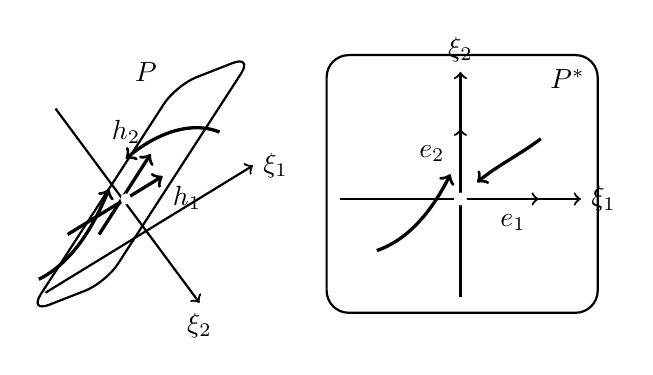
\begin{tikzpicture}[x=0.85cm,y=0.85cm,thick]
  % Oblique plane P and its eigenbasis.
  \draw[rounded corners=8pt] (-4.0,-1.65)--(-1.8,1.75)--(-0.65,2.2)--(-2.85,-1.2)--cycle;
  \coordinate (O) at (-2.55,0.05);
  \draw[->] (-3.75,-1.35)--(-0.65,0.55) node[right] {$\xi_1$};
  \draw[->] (-3.6,1.4)--(-1.45,-1.5) node[below] {$\xi_2$};
  \draw[->,very thick] (-3.42,-0.48)--(-2.0,0.39);
  \draw[->,very thick] (-2.95,-0.48)--(-2.18,0.72);
  \node[below right] at (-2.0,0.39) {$\vect{h}_1$};
  \node[above left] at (-2.18,0.72) {$\vect{h}_2$};
  \fill[white] (O) circle (2pt);
  \node at (-2.25,1.95) {$P$};
  % Sample trajectories in the skew plane.
  \draw[->,very thick] (-3.85,-1.15) .. controls (-3.25,-0.85) and (-2.95,-0.15) .. (-2.8,0.2);
  \draw[->,very thick] (-1.15,1.05) .. controls (-1.65,1.25) and (-2.2,0.95) .. (-2.55,0.65);
  % Affine image P*: orthogonal coordinate axes and corresponding trajectories.
  \draw[rounded corners=8pt] (0.45,-1.65) rectangle (4.5,2.2);
  \draw[->] (0.65,0.05)--(4.25,0.05) node[right] {$\xi_1$};
  \draw[->] (2.45,-1.42)--(2.45,1.95) node[above] {$\xi_2$};
  \draw[->,very thick] (1.2,-0.72) .. controls (1.7,-0.55) and (2.05,-0.08) .. (2.3,0.42);
  \draw[->,very thick] (3.65,0.95) .. controls (3.35,0.72) and (3.0,0.55) .. (2.7,0.3);
  \draw[->] (2.85,0.05)--(3.62,0.05) node[midway,below=2pt] {$\vect{e}_1$};
  \draw[->] (2.45,0.36)--(2.45,1.10) node[midway,left=2pt] {$\vect{e}_2$};
  \fill[white] (2.45,0.05) circle (2.3pt);
  \node at (4.05,1.85) {$P^*$};
\end{tikzpicture}

 \caption{原书图 22：左侧相平面 \(P\) 中的斜交特征方向 \(\vect{h}_1,\vect{h}_2\) 经仿射映射变为
 右侧辅助平面 \(P^*\) 的坐标轴。右侧两条待画轨线在 \(P^*\) 中以 \((\xi_1,\xi_2)\)
 为直角坐标；参数条件是两个特征值为互异实数且都非零。}
 \label{fig:ch2-p2-22}
\end{figure}

在 \(P^*\) 中，除了式 (7) 的轨线外，还分别有由
\begin{equation}
 \xi_1=c_1e^{\lambda_1t},\qquad
 \xi_2=-c_2e^{\lambda_2t}
 \tag{8}
\end{equation}
以及
\begin{equation}
 \xi_1=-c_1e^{\lambda_1t},\qquad
 \xi_2=c_2e^{\lambda_2t}
 \tag{9}
\end{equation}
给出的轨线。式 (7) 关于横轴作镜面反射得到式 (8)；关于纵轴作镜面反射到式 (9)。因此只要画出
第一象限内的轨线，就能利用这两个反射补出整个 \(P^*\)。若 \(c_1=c_2=0\)，得到原点
平衡位置；若 \(c_2=0,c_1>0\)，点在正半横轴上运动；若 \(c_1=0,c_2>0\)，点在正半纵轴
上运动。当 \(\lambda_1<0\) 时，横轴上的点朝原点运动；当 \(\lambda_1>0\) 时，点背离
原点而向无穷远运动。纵轴同理。只要 \(c_1,c_2>0\)，第一象限内的点不会越出象限边界，
因为两个坐标的指数因子都保持正号。

\subsection*{结点和鞍点}
\addcontentsline{toc}{subsection}{结点和鞍点}

\begin{sourceitem}{命题 (A)}
设 \(\lambda_1,\lambda_2\) 都非零且同号，并按绝对值大小编号，使
\begin{equation}
 |\lambda_1|<|\lambda_2|.
 \tag{10}
\end{equation}
若
\[
 \lambda_1<0,\qquad\lambda_2<0,
\]
则相图称为稳定结点；若
\[
 \lambda_1>0,\qquad\lambda_2>0,
\]
则称为不稳定结点。
\end{sourceitem}

以稳定结点为例。沿正半横轴的解为
\(\vect{\xi}(t)=(c_1e^{\lambda_1t},0)\)，沿正半纵轴的解为
\((0,c_2e^{\lambda_2t})\)，两者都随 \(t\) 增大而趋近原点。在第一象限内部，假设
\(c_1,c_2>0\)，则
\[
 \xi_1=c_1e^{\lambda_1t},\qquad
 \xi_2=c_2e^{\lambda_2t}.
\]
因为 \(\lambda_2\) 更负，纵坐标衰减更快，所以曲线在原点处与横轴相切；当
\(t\to-\infty\) 时，两个坐标都增大，但纵坐标增长更快，因此远处的运动方向更偏向纵轴。
把第一象限的曲线经平面反射平移，得到全平面图，即图 23(a)。若把两个指数同时反向，
轨线形状不变而运动方向反转，得到不稳定结点，见图 23(b)。

\begin{figure}[H]
 \centering
 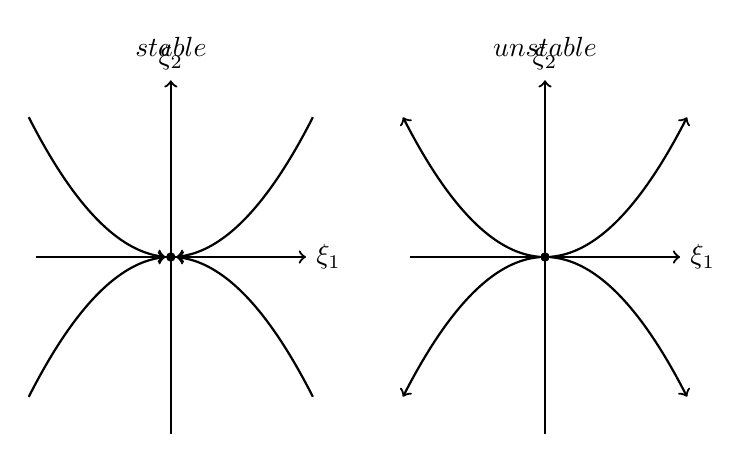
\begin{tikzpicture}[x=0.88cm,y=0.88cm,thick]
  \foreach \cx/\title in {-2.7/stable,2.7/unstable} {
    \draw[->] (\cx-1.95,0)--(\cx+1.95,0) node[right] {$\xi_1$};
    \draw[->] (\cx,-2.55)--(\cx,2.55) node[above] {$\xi_2$};
    \node[above] at (\cx,2.75) {$\title$};
    \fill (\cx,0) circle (1.7pt);
  }
  % Curves are tangent to the slow horizontal eigendirection at the node.
  \foreach \sgnx in {-1,1} {\foreach \sgny in {-1,1} {
    \draw[->] plot[domain=2.05:0.08,samples=65,variable=\s]
      ({-2.7+\sgnx*\s},{\sgny*0.48*\s*\s});
    \draw[->] plot[domain=0.08:2.05,samples=65,variable=\s]
      ({2.7+\sgnx*\s},{\sgny*0.48*\s*\s});
  }}
\end{tikzpicture}

 \caption{原书图 23：辅助平面 \(P^*\) 中的结点。两轴为特征方向；两幅图都满足
 \(|\lambda_1|<|\lambda_2|\) 且特征值同号。左图 \(\lambda_1,\lambda_2<0\)，箭头
 指向原点，是稳定结点；右图 \(\lambda_1,\lambda_2>0\)，箭头背离原点，是不稳定结点。
 曲线在原点处切于横轴，说明衰减较慢的 \(\lambda_1\) 方向占主导。}
 \label{fig:ch2-p2-23}
\end{figure}

\begin{sourceitem}{命题 (B)}
若 \(\lambda_1,\lambda_2\) 异号，则两类坐标一个衰减、一个增长。为确定起见设
\begin{equation}
 \lambda_1<0<\lambda_2.
 \tag{11}
\end{equation}
沿正半横轴的解走向原点，而沿正半纵轴的解离开原点。第一象限内的轨线是双曲线型曲线：
沿稳定方向 \(\xi_2=0\) 趋近原点，沿不稳定方向 \(\xi_1=0\) 离开原点。这个相图称为
鞍点。
\end{sourceitem}

辅助平面的标准图形即图 24。

\begin{figure}[H]
 \centering
 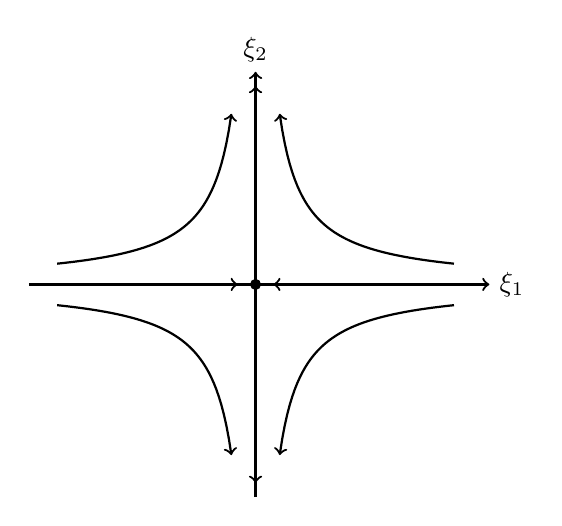
\begin{tikzpicture}[x=0.9cm,y=0.9cm,thick]
  \draw[->] (-3.2,0)--(3.3,0) node[right] {$\xi_1$};
  \draw[->] (0,-3.0)--(0,3.0) node[above] {$\xi_2$};
  % Stable horizontal and unstable vertical separatrices.
  \draw[->] (-2.8,0)--(-0.25,0); \draw[->] (2.8,0)--(0.25,0);
  \draw[->] (0,0.25)--(0,2.8); \draw[->] (0,-0.25)--(0,-2.8);
  % Hyperbolas: forward motion goes from the stable direction toward the unstable one.
  \foreach \sx in {-1,1} {\foreach \sy in {-1,1} {
    \draw[->] plot[domain=2.8:0.34,samples=70,variable=\s]
      ({\sx*\s},{\sy*0.82/\s});
  }}
  \fill (0,0) circle (2pt);
\end{tikzpicture}

 \caption{原书图 24：\(P^*\) 中的鞍点，参数条件为
 \(\lambda_1<0<\lambda_2\)。横轴 \(\xi_2=0\) 是稳定特征方向，箭头从左右两侧指向原点；
 纵轴 \(\xi_1=0\) 是不稳定特征方向，箭头从原点向外。双曲线型轨线先靠近一条特征方向，
 再转向另一条。}
 \label{fig:ch2-p2-24}
\end{figure}

图 23 与图 24 都是辅助平面 \(P^*\) 中的标准图。回到原相平面 \(P\) 时，特征向量的夹角
和长度会改变图形，所以结点可能看起来倾斜，鞍点的两条渐近特征线也未必垂直。图 25、26
给出这种仿射变形：轨线的拓扑类型不变，但弯曲程度和夹角会随 \(\vect{h}_1,\vect{h}_2\) 改变。尤其当
两个特征向量接近共线时，标准图形在 \(P\) 中会被拉得很窄，不能只凭视觉角度判断矩阵结构。

\begin{figure}[H]
 \centering
 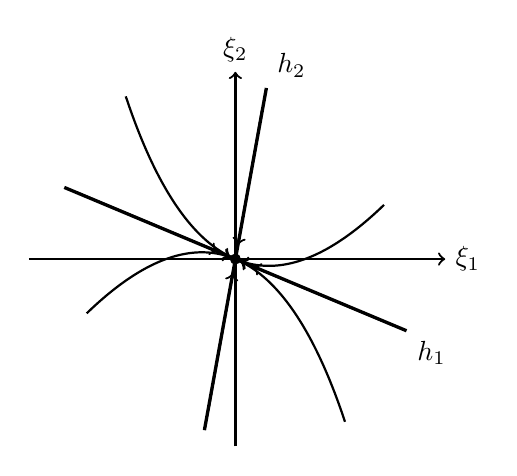
\begin{tikzpicture}[x=0.82cm,y=0.82cm,thick]
  % Stable node in a skew eigenbasis; h1 is the slow direction.
  \draw[->] (-3.2,0)--(3.25,0) node[right] {$\xi_1$};
  \draw[->] (0,-2.9)--(0,2.9) node[above] {$\xi_2$};
  \draw[very thick] (-2.65,1.11)--(2.65,-1.11) node[below right] {$\vect{h}_1$};
  \draw[very thick] (-0.48,-2.65)--(0.48,2.65) node[above right] {$\vect{h}_2$};
  \draw[->] (-2.45,1.03)--(-0.28,0.12); \draw[->] (2.45,-1.03)--(0.28,-0.12);
  \draw[->] (-0.42,-2.35)--(-0.04,-0.22); \draw[->] (0.42,2.35)--(0.04,0.22);
  % Plot v = C u^2 in eigen-coordinates, then shear it into the physical plane.
  \foreach \su in {-1,1} {\foreach \sv in {-1,1} {
    \draw[->] plot[domain=2.0:0.08,samples=65,variable=\s]
      ({\su*\s+0.18*\sv*0.42*\s*\s},{-0.42*\su*\s+\sv*0.42*\s*\s});
  }}
  \fill (0,0) circle (2pt);
\end{tikzpicture}

 \caption{原书图 25：相平面 \(P\) 中的稳定结点，坐标轴是特征方向
 \(\xi_1,\xi_2\) 的像。参数为 \(\lambda_1,\lambda_2<0\)，两个特征方向不垂直；
 轨线在原点附近偏向衰减较慢的特征方向。}
 \label{fig:ch2-p2-25}
\end{figure}

\begin{figure}[H]
 \centering
 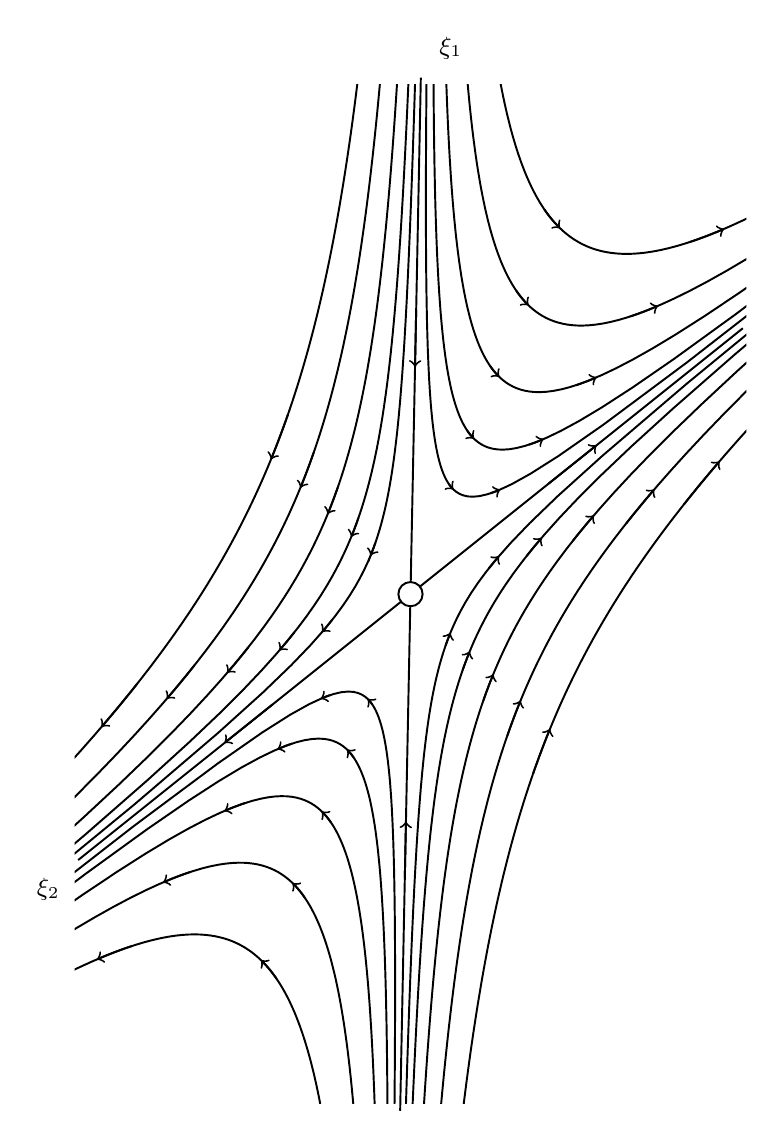
\begin{tikzpicture}[scale=2.5729,font=\small,x=0.85cm,y=0.85cm,line width=0.7pt]
  % Saddle: u'=-u, v'=v; h_1=(0.02,1), h_2=(-1,-0.8).
  % Thus x=0.02u-v, y=u-0.8v and u*v is constant along each orbit.
  \begin{scope}
    \clip (-1.95,-2.96) rectangle (1.95,2.96);
    \foreach \su in {-1,1} {
      \foreach \sv in {-1,1} {
        \foreach \k in {0.10,0.22,0.43,0.76,1.22} {
          \draw plot[domain=0.035:6,samples=220,variable=\s]
            ({0.02*\su*\s-\sv*\k/\s},
             {\su*\s-0.8*\sv*\k/\s});
          \foreach \m in {0.65,1.40} {
            \draw[->] plot[domain={1.06*\m*sqrt(\k)}:{0.94*\m*sqrt(\k)},
              samples=9,variable=\s]
              ({0.02*\su*\s-\sv*\k/\s},
               {\su*\s-0.8*\sv*\k/\s});
          }
        }
      }
    }
  \end{scope}
  \draw (-0.060,-3)--(0.060,3);
  \draw (-1.93,-1.544)--(1.93,1.544);
  \foreach \sgn in {-1,1} {
    \draw[->] ({0.02*1.65*\sgn},{1.65*\sgn})
      --({0.02*1.32*\sgn},{1.32*\sgn});
    \draw[->] ({0.80*\sgn},{0.64*\sgn})
      --({1.08*\sgn},{0.864*\sgn});
  }
  \fill[white] (0,0) circle (1.7pt);
  \draw (0,0) circle (1.7pt);
  \node[above right=3pt] at (0.060,3) {$\xi_1$};
  \node[below left=3pt] at (-1.93,-1.544) {$\xi_2$};
\end{tikzpicture}

 \caption{原书图 26：相平面 \(P\) 中的鞍点，坐标轴是特征方向
 \(\xi_1,\xi_2\) 的像。参数为 \(\lambda_1<0<\lambda_2\)，两条特征直线不垂直；
 箭头沿稳定特征方向趋近原点，并沿不稳定特征方向离开原点。}
 \label{fig:ch2-p2-26}
\end{figure}

\subsection*{焦点和中心}
\addcontentsline{toc}{subsection}{焦点和中心}

\begin{sourceitem}{命题 (C)}
现在考察矩阵有一对非实复共轭特征值的情形。写成
\begin{equation}
 \lambda=\mu+i\nu,\qquad
 \overline\lambda=\mu-i\nu,\qquad \nu\neq0.
 \tag{12}
\end{equation}
特征向量也可以选成共轭
\(\vect{h}\) 与 \(\overline{\vect{h}}\)。把
\[
 \vect{h}=\frac12(\vect{h}_1-i\vect{h}_2)
\]
中的 \(\vect{h}_1,\vect{h}_2\) 取为实向量；可以证明 \(\vect{h}_1,\vect{h}_2\) 线性无关。若它们线性相关，则 \(\vect{h}\)
与 \(\overline{\vect{h}}\) 也线性相关，这与复特征向量不属于同一个一维实方向相矛盾。因此
\((\vect{h}_1,\vect{h}_2)\) 可以作为实相平面 \(P\) 的一组基。

任一实解写成
\begin{equation}
 \vect{x}=c\,\vect{h} e^{\lambda t}
  +\overline c\,\overline{\vect{h}} e^{\overline\lambda t},
 \tag{13}
\end{equation}
其中 \(c\) 是复常数。令
\[
 \zeta=\xi_1+i\xi_2,\qquad
 \xi_1+i\xi_2=c e^{\lambda t}.
\]
于是
\[
 \vect{x}=\xi_1\vect{h}_1+\xi_2\vect{h}_2.
\]
把相平面 \(P\) 仿射映射到变量 \(\zeta\) 的辅助平面 \(P^*\)，使 \(\vect{h}_1\) 的端点变到
\(1\)，使 \(\vect{h}_2\) 的端点变到 \(i\)。则 \(\xi_1\vect{h}_1+\xi_2\vect{h}_2\) 对应
\(\xi_1+i\xi_2=\zeta\)，相轨线满足
\begin{equation}
 \zeta(t)=c e^{\lambda t}.
 \tag{14}
\end{equation}

把式 (14) 写成极坐标。令
\[
 \zeta=\rho e^{i\varphi},\qquad
 c=Re^{i\alpha}.
\]
则
\begin{equation}
 \rho(t)=Re^{\mu t},\qquad
 \varphi(t)=\nu t+\alpha.
 \tag{15}
\end{equation}
当 \(\mu\neq0\) 时，\(P^*\) 中每条轨线都是对数螺线；原相平面 \(P\) 中经仿射变形后的
对应图形称为焦点。若 \(\mu<0\)，当 \(t\) 增大时点沿螺线渐近地趋向原点，称为稳定焦点，
见图 27(a)。若 \(\mu>0\)，点离开原点而趋于无穷，称为不稳定焦点，见图 27(b)。

\begin{figure}[H]
 \centering
 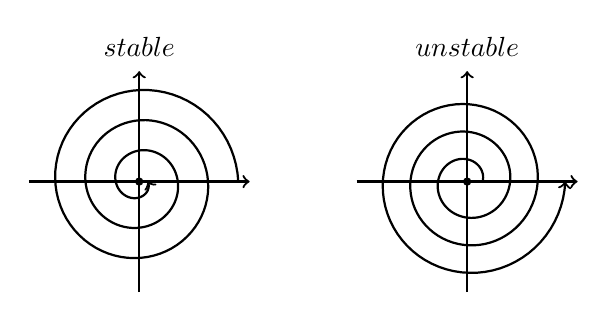
\begin{tikzpicture}[x=0.85cm,y=0.85cm,thick]
  \foreach \cx/\sgn/\title in {-2.45/-1/stable,2.45/1/unstable} {
    \draw[->] (\cx-1.65,0)--(\cx+1.65,0); \draw[->] (\cx,-1.65)--(\cx,1.65);
    \node[above] at (\cx,1.72) {$\title$}; \fill (\cx,0) circle (1.5pt);
  }
  \draw[->] plot[domain=0:1080,samples=220,variable=\t] ({-2.45+1.48*(1-\t/1180)*cos(\t)},{1.48*(1-\t/1180)*sin(\t)});
  \draw[->] plot[domain=0:1080,samples=220,variable=\t] ({2.45+(0.23+0.00115*\t)*cos(\t)},{(0.23+0.00115*\t)*sin(\t)});
\end{tikzpicture}

 \caption{原书图 27：辅助平面 \(P^*\) 中的焦点。横轴为 \(\xi_1\)，纵轴为
 \(\xi_2\)，\(\lambda=\mu\pm i\nu\) 且 \(\nu\neq0\)。左图 \(\mu<0\)，螺线随
 \(t\) 增大而向原点收紧，是稳定焦点；右图 \(\mu>0\)，螺线向外扩展，是不稳定焦点。}
 \label{fig:ch2-p2-27}
\end{figure}

若 \(\mu=0\)，则 \(\rho(t)=R\) 为常数，\(\varphi(t)=\nu t+\alpha\) 线性变化。除平衡
位置 \((0,0)\) 外，每条轨线都是闭圆；这样的相图称为中心，见图 28。中心不是
稳定焦点或渐近稳定平衡位置：解不趋近原点，只是周期地绕行。
\end{sourceitem}

\begin{figure}[H]
 \centering
 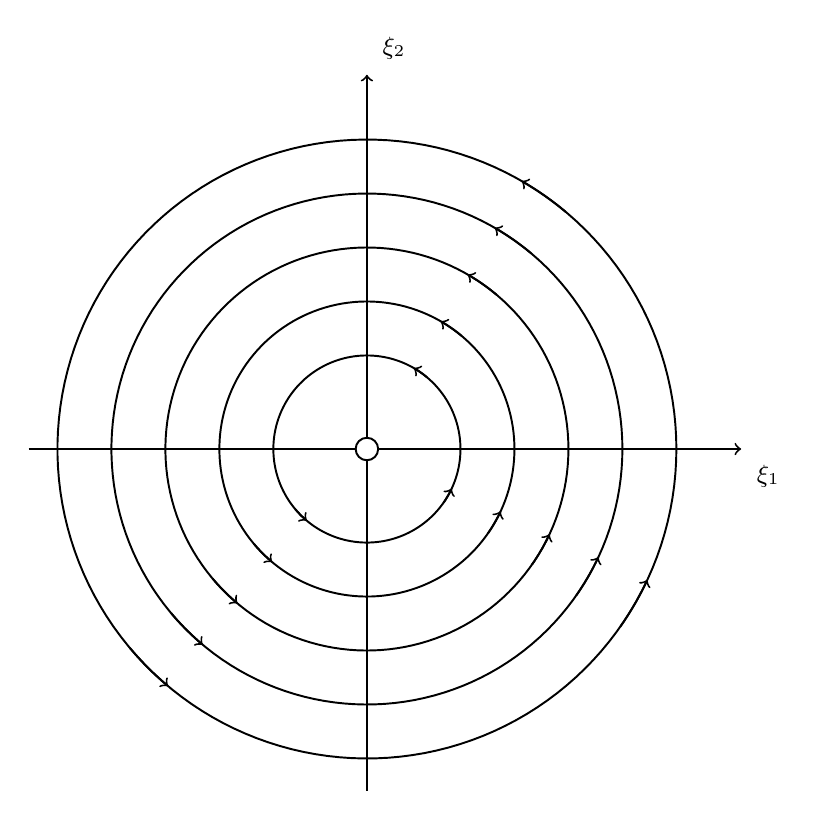
\begin{tikzpicture}[scale=2.5390,font=\small,x=0.9cm,y=0.9cm,line width=0.7pt]
  % xi_1'=-xi_2, xi_2'=xi_1: concentric counterclockwise periodic orbits.
  \foreach \r in {0.52,0.82,1.12,1.42,1.72} {
    \draw plot[domain=0:360,samples=160,variable=\a]
      ({\r*cos(\a)},{\r*sin(\a)})--cycle;
    \foreach \b in {55,225,330} {
      \draw[->] plot[domain={\b-5}:{\b+5},samples=9,variable=\a]
        ({\r*cos(\a)},{\r*sin(\a)});
    }
  }
  \draw[->] (-1.88,0)--(2.08,0);
  \draw[->] (0,-1.90)--(0,2.08);
  \fill[white] (0,0) circle (1.6pt);
  \draw (0,0) circle (1.6pt);
  \node[below right=2pt] at (2.08,0) {$\xi_1$};
  \node[above right=2pt] at (0,2.08) {$\xi_2$};
\end{tikzpicture}

 \caption{原书图 28：辅助平面 \(P^*\) 中的中心，横轴为 \(\xi_1\)、纵轴为
 \(\xi_2\)，参数条件是 \(\mu=0,\nu\neq0\)。所有非零轨线都是以原点为圆心的闭环，
 箭头方向由 \(\nu\) 的符号决定；这里每圈半径由初值 \(|c|\) 保持不变。}
 \label{fig:ch2-p2-28}
\end{figure}

图 27、28 给出 \(P^*\) 中的标准图形。回到 \(P\) 后，圆和螺线被仿射地拉成椭圆、螺线形
椭圆。图 29、30 说明这种变形：中心的同心圆可以变成同心椭圆，焦点的螺线也可以被拉斜，
但闭合与趋近原点的性质不变。

\begin{figure}[H]
 \centering
 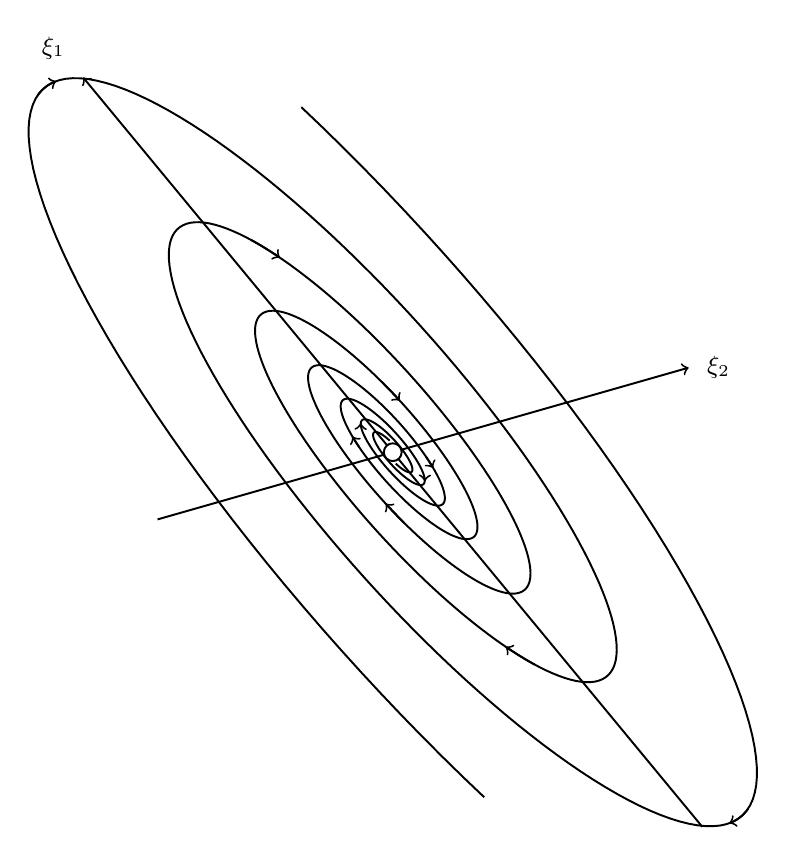
\begin{tikzpicture}[scale=2.1413,font=\small,x=0.9cm,y=0.9cm,line width=0.7pt]
  % Two centrally inverted stable logarithmic spirals under one affine map.
  % P=[(-0.95,1.15)^T,(0.42,0.12)^T], rho=3 exp(-0.0027(a-55)).
  \foreach \sgn in {-1,1} {
    \draw plot[domain=55:1315,samples=500,variable=\a]
      ({\sgn*3*exp(-0.0027*(\a-55))*(-0.95*cos(\a)+0.42*sin(\a))},
       {\sgn*3*exp(-0.0027*(\a-55))*(1.15*cos(\a)+0.12*sin(\a))});
    \foreach \j in {110,330,550,770,990} {
      \draw[->] plot[domain={55+\j-5}:{55+\j+5},samples=9,variable=\a]
        ({\sgn*3*exp(-0.0027*(\a-55))*(-0.95*cos(\a)+0.42*sin(\a))},
         {\sgn*3*exp(-0.0027*(\a-55))*(1.15*cos(\a)+0.12*sin(\a))});
    }
  }
  % Original coordinate images only: positive xi_1 is NW, positive xi_2 is NE.
  \draw[->] (2.04,-2.469)--(-2.04,2.469);
  \draw[->] (-1.55,-0.443)--(1.95,0.557);
  \fill[white] (0,0) circle (1.5pt);
  \draw (0,0) circle (1.5pt);
  \node[above left=3pt] at (-2.04,2.469) {$\xi_1$};
  \node[right=3pt] at (1.95,0.557) {$\xi_2$};
\end{tikzpicture}

 \caption{原书图 29：相平面 \(P\) 中由焦点经仿射变形得到的稳定螺旋。斜轴标出
 \(\xi_1,\xi_2\) 的像；参数为 \(\mu<0,\nu\neq0\)，沿轨线的箭头随 \(t\) 增大而向
 原点收紧。}
 \label{fig:ch2-p2-29}
\end{figure}

\begin{figure}[H]
 \centering
 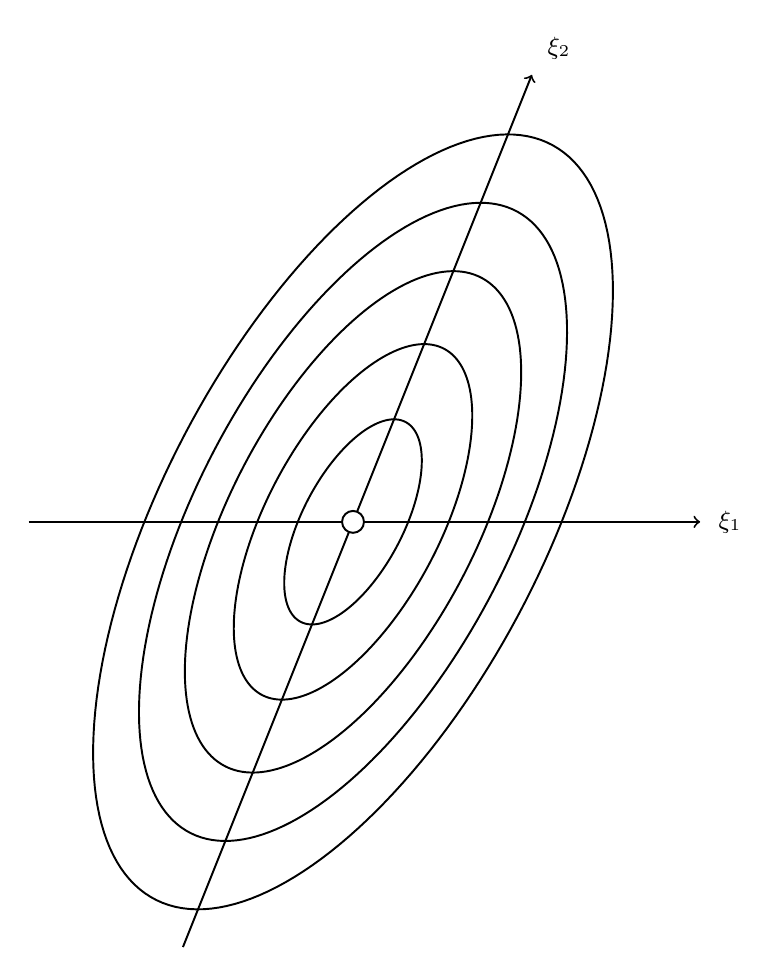
\begin{tikzpicture}[scale=2.4742,font=\small,x=0.9cm,y=0.9cm,line width=0.7pt]
  % Affine image of u'=-v, v'=u under P=[(0.70,0)^T,(0.52,1.30)^T].
  % The source shows closed orbits without flow arrows.
  \foreach \r in {0.45,0.78,1.10,1.40,1.70} {
    \draw plot[domain=0:360,samples=180,variable=\a]
      ({\r*(0.70*cos(\a)+0.52*sin(\a))},{1.30*\r*sin(\a)})--cycle;
  }
  \draw[->] (-1.85,0)--(1.98,0);
  \draw[->] (-0.97,-2.425)--(1.02,2.55);
  \fill[white] (0,0) circle (1.6pt);
  \draw (0,0) circle (1.6pt);
  \node[right=3pt] at (1.98,0) {$\xi_1$};
  \node[above right=2pt] at (1.02,2.55) {$\xi_2$};
\end{tikzpicture}

 \caption{原书图 30：相平面 \(P\) 中的中心经仿射变形得到的同心椭圆族。斜轴标出
 \(\xi_1,\xi_2\) 的像；参数为 \(\mu=0,\nu\neq0\)，每个椭圆都是闭轨线，运动方向由
 \(\nu\) 的符号决定。}
 \label{fig:ch2-p2-30}
\end{figure}

以上讨论的是非退化情形：\(\lambda_1,\lambda_2\) 不相等且都不为零。矩阵元素作足够小的
扰动时，结点、鞍点和焦点的基本相图通常保持不变；中心是例外。中心条件
\(\operatorname{tr}\mat{A}=0,\det \mat{A}>0\) 只是一个等式条件，微扰可能使实部变为负或正，于是
中心分裂成稳定焦点或不稳定焦点。这就是中心的结构不稳定性。其他退化情形，即重根或至少
一个零特征值，将在下面例题 1 和例题 3 中讨论。

\subsection*{例题}

\paragraph{例 1：退化结点.}
设方程组 (2) 的矩阵 \(\mat{A}\) 只有一个特征值 \(\lambda\)。二重特征值并
不自动意味着矩阵可对角化，因此有两种本质上不同的情形。以下用 \(\mat{A}\) 同时表示矩阵和它
所定义的线性变换。

\medskip
\noindent\textbf{情形 I.}
相平面 \(P\) 中存在由两个特征向量组成的基 \(\vect{h}_1,\vect{h}_2\)，使
\begin{equation}
 \mat{A}\vect{h}_1=\lambda \vect{h}_1,\qquad
 \mat{A}\vect{h}_2=\lambda \vect{h}_2.
 \tag{16}
\end{equation}
这等价于 \(\mat{A}=\lambda \mat{I}\) 在其特征基下可对角化，因而几何重数等于二。

\medskip
\noindent\textbf{情形 II.}
相平面中存在一组基 \(\vect{h}_1,\vect{h}_2\)，使
\begin{equation}
 \mat{A}\vect{h}_1=\lambda \vect{h}_1,\qquad
 \mat{A}\vect{h}_2=\lambda \vect{h}_2+\vect{h}_1.
 \tag{17}
\end{equation}
这时 \(\vect{h}_2\) 是二级广义特征向量，\((\vect{h}_1,\vect{h}_2)\) 是一条长度为一的 Jordan 链。

一般 Jordan 标准形定理直接保证两种基至少有一种存在。这里也可以直接验证。先取
\(\vect{h}_1\neq\vect{0}\) 为特征向量，再取任意与 \(\vect{h}_1\) 不共线的 \(\vect{h}_2\)。因为
\(\vect{h}_1,\vect{h}_2\) 构成基，可写
\[
 \mat{A}\vect{h}_2=a \vect{h}_1+\mu \vect{h}_2.
\]
在这组基下，变换矩阵为
\[
 \begin{pmatrix}
  \lambda&a\\
  0&\mu
 \end{pmatrix}.
\]
它的特征值为 \(\lambda,\mu\)，而根据假设只有唯一特征值 \(\lambda\)，所以
\(\mu=\lambda\)。若 \(a=0\)，就是情形 I。若 \(a\neq0\)，把 \(\vect{h}_1\) 换成
\(a \vect{h}_1\)；这个向量仍属于同一特征空间，并且
\[
 \mat{A} \vect{h}_2=\lambda \vect{h}_2+a \vect{h}_1
 =\lambda \vect{h}_2+(a \vect{h}_1),
\]
于是得到情形 II 的关系式 (17)。

在情形 I 中，通解可以直接写成
\begin{equation}
 \vect{x}(t)=c_1\vect{h}_1e^{\lambda t}+c_2\vect{h}_2e^{\lambda t}
 =\vect{x}_0e^{\lambda t}.
 \tag{18}
\end{equation}
只要 \(\vect{x}_0\neq\vect{0}\)，\(\lambda\neq0\) 时每个解都沿过原点、方向为 \(\vect{x}_0\) 的半射线
运动。\(\lambda<0\) 时朝原点运动，\(\lambda>0\) 时离开原点。每条由初值决定的射线本身
是一条轨线；与通常的稳定结点不同，这里没有另一条趋于较慢的特征方向，而是所有方向都以
相同指数速率伸缩。

\begin{figure}[H]
 \centering
 \begin{tikzpicture}[scale=1.7587,font=\small,x=.82cm,y=.82cm,line width=.65pt,>=Stealth]
  % Scalar matrices: every half-ray is a complete trajectory.
  \foreach \cx/\sense/\panel in {-2.8/in/a,2.8/out/b} {
    \begin{scope}[shift={(\cx,0)}]
      \foreach \ang in {0,22.5,...,337.5} {
        \draw ({.055*cos(\ang)},{.055*sin(\ang)})
          --({2.18*cos(\ang)},{2.18*sin(\ang)});
        \def\inward{in}
        \ifx\sense\inward
          \draw[->] ({1.55*cos(\ang)},{1.55*sin(\ang)})
            --({1.10*cos(\ang)},{1.10*sin(\ang)});
        \else
          \draw[->] ({.92*cos(\ang)},{.92*sin(\ang)})
            --({1.40*cos(\ang)},{1.40*sin(\ang)});
        \fi
      }
      \filldraw[fill=white,line width=.45pt] (0,0) circle (1.5pt);
      \node[below] at (0,-2.38) {(\panel)};
    \end{scope}
  }
\end{tikzpicture}

 \caption{原书图 31：例 1 情形 I 的二重特征值、可对角化情形。左图
 \(\lambda<0\)，沿每条从原点出发的半射线向内运动，原点为稳定退化结点，而且不出现
 螺旋项；右图 \(\lambda>0\)，方向反转，所有点向外运动。此情形在二维中正是
 \(\mat{A}=\lambda \mat{I}\)；图中所有半射线都是轨线。}
 \label{fig:ch2-p2-31}
\end{figure}

在情形 II 中，任意解都可写成
\begin{equation}
 \vect{x}(t)=c_1\vect{h}_1e^{\lambda t}
      +c_2(t\vect{h}_1+\vect{h}_2)e^{\lambda t}.
 \tag{19}
\end{equation}
把它按基 \((\vect{h}_1,\vect{h}_2)\) 展开为
\(\vect{x}=\xi_1\vect{h}_1+\xi_2\vect{h}_2\)，得到
\begin{equation}
 \xi_1(t)=(c_1+c_2t)e^{\lambda t},\qquad
 \xi_2(t)=c_2e^{\lambda t}.
 \tag{20}
\end{equation}
由于 \(\vect{h}_1,\vect{h}_2\) 可能不垂直，仿射映射把 \(P\) 送到辅助平面 \(P^*\)，并把 \(\vect{h}_1,\vect{h}_2\)
变成沿两个坐标轴的互相正交单位向量。在 \(P^*\) 中，式 (20) 给出
普通直角坐标下的轨线；回到 \(P\) 时再作仿射变形。

以下讨论 \(\lambda\neq0\)，\(\lambda=0\) 见例题 3。由于同时改变 \(c_1,c_2\) 的符号
把 \(P^*\) 中的点关于原点中心对称，并把轨线送到轨线，所以只要研究上半平面的轨线。
当 \(c_2=0,c_1\neq0\) 时，得到两条与横轴重合的轨线：正半横轴和负半横轴，两者都朝原点
运动。再取 \(c_1=0,c_2>0\)，得到
\begin{equation}
 \xi_1(t)=c_2te^{\lambda t},\qquad
 \xi_2(t)=c_2e^{\lambda t}.
 \tag{21}
\end{equation}

当 \(t=0\) 时，点在纵轴上的 \((0,c_2)\)。随着 \(t\) 从零增大，纵坐标以指数速度下降，
而横坐标 \(c_2te^{\lambda t}\) 先向右、随后在 \(t=-1/\lambda\) 处转向左；但整条轨线
始终向原点弯曲，并在原点处与正横轴相切。当 \(t\) 从零减到 \(-\infty\) 时，纵坐标变得
很大，横坐标为负且绝对值增长更快，整体趋势朝向负横轴。让 \(c_2\) 取遍所有正值，这样
的轨线填满上半平面。当 \(\lambda<0\) 时，所有箭头都指向原点，称为稳定的退化结点。

\begin{figure}[H]
 \centering
 \begin{tikzpicture}[x=0.76cm,y=0.76cm,thick,>=Stealth]
  % Auxiliary Jordan coordinates: trajectories are tangent to the xi_1 axis.
  \begin{scope}[shift={(-2.35,0)}]
    \draw[thin] (-1.8,0)--(1.8,0) node[right] {$\xi_1$};
    \draw[thin] (0,-1.7)--(0,1.7) node[above] {$\xi_2$};
    \node[above] at (0,2.28) {$stable$};
    \fill (0,0) circle (1.4pt);
    % Stable flow along the eigendirection.
    \draw[->] (-1.55,0)--(-0.28,0);
    \draw[<-] (0.28,0)--(1.55,0);
    % Upper trajectories enter from the left, bend around, then approach tangent to xi_1.
    \draw[->] (-2.15,1.50).. controls (-1.55,1.70) and (0.95,0.03)..(0.16,0.03);
    \draw[->] (-1.80,1.08).. controls (-1.25,1.25) and (0.70,0.02)..(0.14,0.02);
    \draw[->] (-1.45,0.68).. controls (-0.98,0.80) and (0.48,0.01)..(0.12,0.01);
    % Lower trajectories are the reflected family.
    \draw[->] (2.15,-1.50).. controls (1.55,-1.70) and (-0.95,-0.03)..(-0.16,-0.03);
    \draw[->] (1.80,-1.08).. controls (1.25,-1.25) and (-0.70,-0.02)..(-0.14,-0.02);
    \draw[->] (1.45,-0.68).. controls (0.98,-0.80) and (-0.48,-0.01)..(-0.12,-0.01);
  \end{scope}
  \begin{scope}[shift={(2.35,0)}]
    \draw[thin] (-1.8,0)--(1.8,0) node[right] {$\xi_1$};
    \draw[thin] (0,-1.7)--(0,1.7) node[above] {$\xi_2$};
    \node[above] at (0,2.28) {$unstable$};
    \fill (0,0) circle (1.4pt);
    % Reverse every arrow for the unstable case.
    \draw[<-] (-1.55,0)--(-0.28,0);
    \draw[->] (0.28,0)--(1.55,0);
    \draw[<-] (-2.15,1.50).. controls (-1.55,1.70) and (0.95,0.03)..(0.16,0.03);
    \draw[<-] (-1.80,1.08).. controls (-1.25,1.25) and (0.70,0.02)..(0.14,0.02);
    \draw[<-] (-1.45,0.68).. controls (-0.98,0.80) and (0.48,0.01)..(0.12,0.01);
    \draw[<-] (2.15,-1.50).. controls (1.55,-1.70) and (-0.95,-0.03)..(-0.16,-0.03);
    \draw[<-] (1.80,-1.08).. controls (1.25,-1.25) and (-0.70,-0.02)..(-0.14,-0.02);
    \draw[<-] (1.45,-0.68).. controls (0.98,-0.80) and (-0.48,-0.01)..(-0.12,-0.01);
  \end{scope}
\end{tikzpicture}

 \caption{原书图 32：Jordan 链基下辅助平面 \(P^*\) 的退化结点。坐标轴就是
 \((\vect{h}_1,\vect{h}_2)\) 的像。左图 \(\lambda<0\)，轨线在原点与横轴相切，运动向内，是稳定
 退化结点；右图 \(\lambda>0\)，运动向外，是不稳定退化结点。两幅图都对应二重特征值且
 只有一个独立特征向量。}
 \label{fig:ch2-p2-32}
\end{figure}

若 \(\lambda>0\)，把上面的图形关于纵轴作镜面反射并反转时间方向，就得到不稳定退化结点，
见图 32(b)。图 33(a),(b) 回到原相平面 \(P\)，显示非正交特征基造成的倾斜变形。相切的
方向仍然是唯一的特征直线 \(\vect{h}_1\)；另一条 Jordan 方向的像 \(\vect{h}_2\) 只决定曲线从哪一侧
接入。

\begin{figure}[H]
 \centering
 \begin{tikzpicture}[scale=1.1900,font=\small,line width=.65pt,>=Stealth]
  % The two original panels use different oblique bases.  Each is a
  % linear image of the exact Jordan portrait of Figure 32.
  \begin{scope}[shift={(-3.0,0)},x={(.58cm,.92cm)},y={(-.35cm,.74cm)}]
    \begin{scope}
      \clip (-2.55,-2.25)--(2.55,-2.25)--(2.55,2.25)--(-2.55,2.25)--cycle;
      \foreach \a in {.55,1.05,1.60} {
        \foreach \sgn in {-1,1} {
          \draw plot[domain=-1.5:8,samples=190,variable=\t]
            ({\sgn*2.7*\a*\t*exp(-\t)},{\sgn*\a*exp(-\t)});
          \foreach \ta/\tb in {-.28/-.12,.65/.82} {
            \draw[->] plot[domain=\ta:\tb,samples=12,variable=\t]
              ({\sgn*2.7*\a*\t*exp(-\t)},{\sgn*\a*exp(-\t)});
          }
        }
      }
    \end{scope}
    \draw[line width=.45pt] (-2.70,0)--(2.70,0)
      node[above right,xshift=2pt] {$\xi_1$};
    \draw[line width=.45pt] (0,-2.30)--(0,2.30)
      node[above left,xshift=-2pt] {$\xi_2$};
    \draw[->] (-2.2,0)--(-1.75,0);
    \draw[->] (2.2,0)--(1.75,0);
    \filldraw[fill=white,line width=.45pt] (0,0) circle (1.5pt);
  \end{scope}
  \node[below] at (-3.0,-2.95) {(a)};
  \begin{scope}[shift={(3.0,0)},x={(.78cm,.78cm)},y={(-1.20cm,0cm)}]
    \begin{scope}
      \clip (-2.55,-2.25)--(2.55,-2.25)--(2.55,2.25)--(-2.55,2.25)--cycle;
      \foreach \a in {.55,1.05,1.60} {
        \foreach \sgn in {-1,1} {
          \draw plot[domain=-1.5:8,samples=190,variable=\t]
            ({-\sgn*2.7*\a*\t*exp(-\t)},{\sgn*\a*exp(-\t)});
          \foreach \ta/\tb in {-.28/-.12,.65/.82} {
            \draw[<-] plot[domain=\ta:\tb,samples=12,variable=\t]
              ({-\sgn*2.7*\a*\t*exp(-\t)},{\sgn*\a*exp(-\t)});
          }
        }
      }
    \end{scope}
    \draw[line width=.45pt] (-2.70,0)--(2.70,0)
      node[above right,xshift=2pt] {$\xi_1$};
    \draw[line width=.45pt] (0,-2.30)--(0,2.30)
      node[left,xshift=-2pt] {$\xi_2$};
    \draw[->] (-1.75,0)--(-2.2,0);
    \draw[->] (1.75,0)--(2.2,0);
    \filldraw[fill=white,line width=.45pt] (0,0) circle (1.5pt);
  \end{scope}
  \node[below] at (3.0,-2.95) {(b)};
\end{tikzpicture}

 \caption{原书图 33：原相平面 \(P\) 中的退化结点。与图 32 相比，坐标轴不再正交，曲线被
 仿射拉斜，但两个特征方向 \(\vect{h}_1,\vect{h}_2\) 仍然保留；轨线在原点附近仍切于特征方向
 \(\vect{h}_1\)。左、右两个图形对应稳定和不稳定两个时间方向。}
 \label{fig:ch2-p2-33}
\end{figure}

\paragraph{例 2：二阶常系数线性齐次方程.}
考虑标量方程
\begin{equation}
 \ddot x+a\dot x+bx=0,
 \qquad a,b\in\R,
 \tag{22}
\end{equation}
其中 \(\dot x\) 表示对时间的导数。按第~\S4 的方法引入状态变量 \((x,\dot x)\)，可写成
标准方程组
\begin{equation}
 \dot x=y,\qquad
 \dot y=-bx-ay.
 \tag{23}
\end{equation}
把 \((x,y)\) 平面看成原方程的相平面。直接计算可知，方程组 (23)
的系数矩阵特征多项式为
\begin{equation}
 p^2+ap+b.
 \tag{24}
\end{equation}
它正好是原二阶方程的特征多项式。因此前面关于相平面的结点、鞍点、焦点和中心结论都可以
直接用于二阶方程。

若式 (24) 的根为复数，则相平面出现焦点或中心。下面讨论两根非零、
互不相同且为实数的情形。设 \(\lambda\) 是根，\(\vect{h}=(h^1,h^2)\neq\vect{0}\) 是对应特征向量。
由方程组 (23) 的形式，
\[
 \lambda h^1=h^2.
\]
因此特征方向由
\begin{equation}
 y=\lambda x
 \tag{25}
\end{equation}
确定；这条直线称为特征直线。这里第一坐标是位移，第二坐标是速度；图中的横轴标为
\(x\)，纵轴标为 \(\dot x\)，两者都是同一标量函数的相位坐标。

若 \(\lambda_1,\lambda_2<0\)，就有稳定结点，见命题 (A)。两条特征直线都经过第二、
第四象限；在原点附近，轨线切于靠近横轴的那条特征直线。其原因是该方向对应的
\(|\lambda|\) 较小，指数衰减较慢，故成为进入原点时的主导方向。图 34 给出这一情形。

\begin{figure}[H]
 \centering
 \begin{tikzpicture}[x=0.8cm,y=0.8cm,thick,>=Stealth]
  \draw[->] (-4.4,0)--(4.4,0) node[right] {$x$};
  \draw[->] (0,-3.5)--(0,3.5) node[above] {$\dot x$};
  % Stable eigenlines: one slow, shallow direction and one fast, steep direction.
  \draw[very thick] (-4.0,1.4)--(4.0,-1.4);
  \draw[very thick] (-2.55,3.45)--(2.55,-3.45);
  \draw[->] (-2.65,0.93)--(-0.24,0.084);
  \draw[->] (2.65,-0.93)--(0.24,-0.084);
  \draw[->] (-1.85,2.50)--(-0.18,0.24);
  \draw[->] (1.85,-2.50)--(0.18,-0.24);
  % Distinct trajectories curve through the upper-left and lower-right sectors.
  % Each approaches the origin tangent to the slower eigendirection.
  \draw[->] (-3.75,2.95).. controls (-3.05,2.75) and (-1.05,0.42)..(-0.14,0.05);
  \draw[->] (-3.35,2.20).. controls (-2.65,2.05) and (-0.92,0.34)..(-0.14,0.05);
  \draw[->] (-3.05,1.45).. controls (-2.35,1.42) and (-0.82,0.29)..(-0.14,0.05);
  \draw[->] (3.75,-2.95).. controls (3.05,-2.75) and (1.05,-0.42)..(0.14,-0.05);
  \draw[->] (3.35,-2.20).. controls (2.65,-2.05) and (0.92,-0.34)..(0.14,-0.05);
  \draw[->] (3.05,-1.45).. controls (2.35,-1.42) and (0.82,-0.29)..(0.14,-0.05);
  \fill (0,0) circle (2pt);
\end{tikzpicture}

 \caption{原书图 34：方程 (24) 的两根皆为负实根时的稳定结点。
 横轴为位移 \(x\)，纵轴为速度 \(\dot x\)；两条斜线是满足 \(\dot x=\lambda x\) 的
 特征直线。所有箭头指向原点，轨线在原点附近切于衰减较慢的特征直线。}
 \label{fig:ch2-p2-34}
\end{figure}

若 \(\lambda_1,\lambda_2>0\)，则有拓扑上的不稳定结点。两条特征直线经过第一、第三象限，
轨线在原点附近仍切于位置较靠近横轴的那条特征直线，但箭头反向，点随时间离开原点。
见图 35。

\begin{figure}[H]
 \centering
 \begin{tikzpicture}[x=0.8cm,y=0.8cm,thick,>=Stealth]
  \draw[->] (-4.4,0)--(4.4,0) node[right] {$x$};
  \draw[->] (0,-3.5)--(0,3.5) node[above] {$\dot x$};
  % Unstable eigenlines have positive slopes.
  \draw[very thick] (-4.0,-1.4)--(4.0,1.4);
  \draw[very thick] (-2.55,-3.45)--(2.55,3.45);
  \draw[->] (0.24,0.084)--(2.65,0.93);
  \draw[->] (-0.24,-0.084)--(-2.65,-0.93);
  \draw[->] (0.18,0.24)--(1.85,2.50);
  \draw[->] (-0.18,-0.24)--(-1.85,-2.50);
  % Reverse-flow companions of the stable-node curves; all arrows leave zero.
  \draw[<-] (3.75,2.95).. controls (3.05,2.75) and (1.05,0.42)..(0.14,0.05);
  \draw[<-] (3.35,2.20).. controls (2.65,2.05) and (0.92,0.34)..(0.14,0.05);
  \draw[<-] (3.05,1.45).. controls (2.35,1.42) and (0.82,0.29)..(0.14,0.05);
  \draw[<-] (-3.75,-2.95).. controls (-3.05,-2.75) and (-1.05,-0.42)..(-0.14,-0.05);
  \draw[<-] (-3.35,-2.20).. controls (-2.65,-2.05) and (-0.92,-0.34)..(-0.14,-0.05);
  \draw[<-] (-3.05,-1.45).. controls (-2.35,-1.42) and (-0.82,-0.29)..(-0.14,-0.05);
  \fill (0,0) circle (2pt);
\end{tikzpicture}

 \caption{原书图 35：方程 (24) 的两根皆为正实根时的不稳定结点。
 横轴 \(x\)、纵轴 \(\dot x\)；两条特征直线 \(\dot x=\lambda_i x\) 均经过第一、第三
 象限，箭头由原点向外。原点附近的主导方向仍是衰减较慢（这里等价于增长较慢）的特征
 直线。}
 \label{fig:ch2-p2-35}
\end{figure}

若两根异号，则原方程为鞍点。两条特征直线中一条经过第二、第四象限，另一条经过第一、
第三象限。轨线沿稳定的特征方向接近原点，而沿不稳定方向离开原点。图 36 给出这一力学
相图；两条双曲线分支的连接方式由 \(b<0\) 和根的符号确定。

\begin{figure}[H]
 \centering
 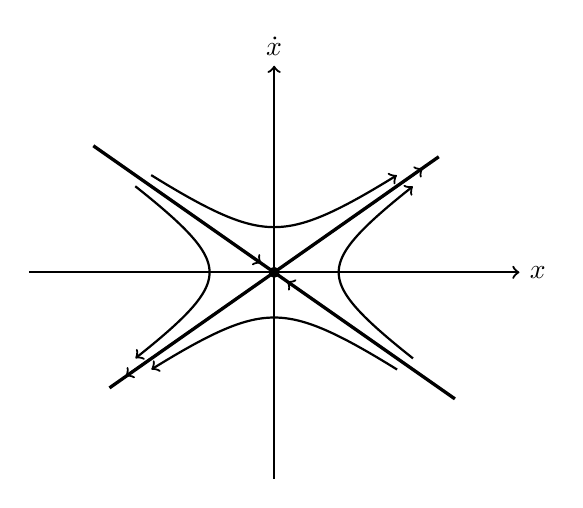
\begin{tikzpicture}[x=0.82cm,y=0.82cm,thick]
  \draw[->] (-3.8,0)--(3.8,0) node[right] {$x$};
  \draw[->] (0,-3.2)--(0,3.2) node[above] {$\dot x$};
  % Stable eigenline has negative slope; unstable eigenline has positive slope.
  \draw[very thick] (-2.8,1.96)--(2.8,-1.96);
  \draw[very thick] (-2.55,-1.79)--(2.55,1.79);
  \draw[->] (-2.5,1.75)--(-0.2,0.14); \draw[->] (2.5,-1.75)--(0.2,-0.14);
  \draw[->] (0.2,0.14)--(2.3,1.61); \draw[->] (-0.2,-0.14)--(-2.3,-1.61);
  % Hyperbolic sample orbits for one negative and one positive eigenvalue.
  \foreach \cOne/\cTwo in {0.5/0.5,0.5/-0.5,-0.5/0.5,-0.5/-0.5} {
    \draw[->] plot[domain=-2:2,samples=140,variable=\t]
      ({\cOne*exp(-0.7*\t)+\cTwo*exp(0.7*\t)},
       {-0.7*\cOne*exp(-0.7*\t)+0.7*\cTwo*exp(0.7*\t)});
  }
  \fill (0,0) circle (2pt);
\end{tikzpicture}

 \caption{原书图 36：方程 (24) 的根一正一负时的相图。横轴为
 \(x\)，纵轴为 \(\dot x\)。一条特征直线经过第二、第四象限，另一条经过第一、第三象限；
 箭头沿前者趋近原点、沿后者离开原点，故为鞍点。}
 \label{fig:ch2-p2-36}
\end{figure}

\paragraph{例 3：至少一个特征值等于零.}

\medskip
\noindent\textbf{情形 I.}
只有一个特征值等于零：
\begin{equation}
 \lambda_1\neq0,\qquad\lambda_2=0.
 \tag{26}
\end{equation}
这时解仍按式 (3) 写，其中
\begin{equation}
 \xi_1(t)=c_1e^{\lambda_1t},\qquad
 \xi_2(t)=c_2.
 \tag{27}
\end{equation}
因为 \(\xi_2=c_2\) 为常数，所有沿固定直线 \(\xi_2=\text{常数}\) 的运动都平行于
\(\xi_1\) 轴；当 \(\lambda_1<0\) 时朝直线 \(\xi_1=0\) 运动，当 \(\lambda_1>0\) 时背离
它运动。直线 \(\xi_1=0\) 上每一点都满足 \(\vect{f}(\vect{x})=\vect{0}\)，因此整条直线由平衡位置组成。
原点不再是唯一平衡位置，所以不能用孤立的结点、鞍点或焦点来称呼这一相图。图 37 给出
辅助平面中的这一结构。

\begin{figure}[H]
 \centering
 \begin{tikzpicture}[scale=2.1634,font=\small,x={(1cm,-.27cm)},y={(.68cm,.74cm)},
  line width=.65pt,>=Stealth]
  % Affine image of xi_1'=lambda_1 xi_1, xi_2'=0, lambda_1<0.
  % The whole oblique xi_2 axis consists of equilibria.
  \foreach \h in {-1.65,-1.10,-.55,.55,1.10,1.65} {
    \draw (-1.90,\h)--(1.90,\h);
    \draw[->] (-1.42,\h)--(-.78,\h);
    \draw[->] (1.42,\h)--(.78,\h);
  }
  \draw[line width=.45pt] (-2.10,0)--(2.10,0)
    node[right,xshift=3pt] {$\xi_1$};
  \draw[->,line width=.55pt] (0,-2.05)--(0,2.05)
    node[above right,xshift=2pt] {$\xi_2$};
  \draw[->] (-1.42,0)--(-.78,0);
  \draw[->] (1.42,0)--(.78,0);
  \filldraw[fill=white,line width=.45pt] (0,0) circle (1.5pt);
\end{tikzpicture}

 \caption{原书图 37：零特征值情形 I，特征值为 \(\lambda_1\neq0,\lambda_2=0\)。
 两条坐标轴为特征方向；直线 \(\xi_1=0\) 上每一点都是平衡位置。轨迹沿水平直线
 \(\xi_2=\text{常数}\) 指向或背离 \(\xi_1=0\)，方向由 \(\lambda_1\) 的符号决定。
 图示 \(\lambda_1<0\)，轨线指向平衡直线；当 \(\lambda_1>0\) 时，所有箭头反向。}
 \label{fig:ch2-p2-37}
\end{figure}

\medskip
\noindent\textbf{情形 II.}
若唯一特征值为
\begin{equation}
 \lambda_1=\lambda_2=0,
 \tag{28}
\end{equation}
则可能分别落在例题 1 的两种情形。

\emph{情形 II.1.} 见关系式 (16) 且 \(\lambda=0\)。通解
(18) 成为
\begin{equation}
 \vect{x}(t)=\vect{x}_0.
 \tag{29}
\end{equation}
这只有当方程组 (1) 的所有系数都等于零时才发生；此时相平面每一点
都是平衡位置，整个平面都是静止的，没有需要分类的轨线。

\emph{情形 II.2.} 见关系式 (17) 且 \(\lambda=0\)。通解
(19) 成为
\begin{equation}
 \xi_1(t)=c_1+c_2t,\qquad
 \xi_2(t)=c_2.
 \tag{30}
\end{equation}
沿着每一条固定直线 \(\xi_2=\text{常数}\)，运动都以常速度 \(c_2\) 进行；当 \(c_2>0\)
时向右，当 \(c_2<0\) 时向左。直线 \(\xi_2=0\) 上所有点都有 \(c_2=0\)，因此都是平衡
位置。图 38 显示这种一维平移的平行轨线族。

\begin{figure}[H]
 \centering
 \begin{tikzpicture}[scale=2.1989,font=\small,x={(.87cm,.22cm)},y={(.12cm,.74cm)},
  line width=.65pt,>=Stealth]
  % Keep the scanned oblique layout; correct its reversed flow arrows
  % according to xi_1'=xi_2, xi_2'=0 in equation (30).
  \foreach \h in {.35,.70,1.05,1.40,1.75,2.10} {
    \draw (-3.10,\h)--(3.10,\h);
    \draw (-3.10,-\h)--(3.10,-\h);
    \foreach \p in {-2.30,-.45,1.40} {
      \draw[->] (\p,\h)--({\p+.55},\h);
      \draw[<-] (\p,-\h)--({\p+.55},-\h);
    }
  }
  \draw[line width=.8pt] (-3.10,0)--(3.10,0)
    node[right,xshift=3pt] {$\xi_1$};
  \draw[line width=.45pt] (0,-2.45)--(0,2.45)
    node[above right,xshift=2pt] {$\xi_2$};
\end{tikzpicture}

 \caption{原书图 38：零特征值且矩阵不可对角化的情形。坐标轴为
 \((\xi_1,\xi_2)\) 的特征链方向；每条水平直线 \(\xi_2=\text{常数}\) 是一条轨线，
 运动匀速并沿 \(\xi_1\) 方向。直线 \(\xi_2=0\) 由平衡位置组成。与图 37 相比，这里
 没有非零指数伸缩，时间依赖是线性的。}
 \label{fig:ch2-p2-38}
\end{figure}

\section*{补证：Hurwitz判据为何成立}
\addcontentsline{toc}{section}{补证：Hurwitz判据为何成立}
\label{sec:hurwitz-proof}

\noindent\textbf{编者补证。}
原书§9只陈述定理7，另引文献给出证明。
为使本稿可独立使用，这里补上证明；它不冒充原书已有的段落。
证明采用与控制理论相通的Routh降阶思路，再把降阶条件写成Hurwitz顺序主子式。
沿用本章已使用的代数事实：固定次数多项式的根作为一个带重数的集合，随系数连续变化。
这不要求能把所有根在全参数范围内逐个编号为单值函数。

\subsection*{1. 奇偶部分与降阶多项式}

设
\[
 P(s)=a_0s^n+a_1s^{n-1}+\cdots+a_n,\qquad a_0>0,
\]
各$a_j$均为实数，且$n\ge2$。
先假定$a_1>0$。把多项式按幂次的奇偶性分成
\[
 U(s)=a_0s^n+a_2s^{n-2}+a_4s^{n-4}+\cdots,
 \qquad
 V(s)=a_1s^{n-1}+a_3s^{n-3}+a_5s^{n-5}+\cdots.
\]
令$c=a_0/a_1>0$，定义
\[
 W(s)=U(s)-csV(s),\qquad Q(s)=V(s)+W(s).
\]
$U$与$csV$的最高次项相消，所以$\deg W\le n-2$，
而$Q$恰为$n-1$次多项式，首项系数$a_1>0$。
写开即为
\[
 Q(s)=a_1s^{n-1}
 +\left(a_2-\frac{a_0a_3}{a_1}\right)s^{n-2}
 +a_3s^{n-3}
 +\left(a_4-\frac{a_0a_5}{a_1}\right)s^{n-4}
 +\cdots.
\]
系数越界时取零。它就是Routh过程的一次降阶。

\subsection*{2. 降阶为什么保持左半平面稳定性}

我们证明
\begin{equation}
 P\text{稳定}
 \quad\Longleftrightarrow\quad
 a_1>0\ \text{且}\ Q\text{稳定}.
 \label{eq:routh-reduction}
\end{equation}
先注意：若$P$稳定，实根给出因子$s+r$，$r>0$；
一对共轭根$-\alpha\pm i\beta$给出
$s^2+2\alpha s+\alpha^2+\beta^2$，$\alpha>0$。
这些因子的系数均为正，故乘积的系数均为正，特别有$a_1>0$。

在$a_1>0$的条件下，考虑实参数族
\[
 P_\tau(s)=W(s)+V(s)+\tau sV(s),\qquad \tau>0.
\]
其中$P_c=P$，而当$\tau\downarrow0$时$P_\tau\to Q$。
对实数$\omega$，$W(i\omega)$与$i\omega V(i\omega)$
都属于同一个实直线$i^n\R$，
$V(i\omega)$则属于与它垂直的实直线$i^{n-1}\R$。
因此
\[
 P_\tau(i\omega)=0
 \quad\Longleftrightarrow\quad
 V(i\omega)=0\ \text{且}\ W(i\omega)=0
 \quad\Longleftrightarrow\quad Q(i\omega)=0.
\]
这个条件与$\tau$无关。
所以，只要$P$或$Q$中一个没有虚轴根，整个$\tau>0$的多项式族都没有虚轴根。

在任意闭参数区间$0<\tau_1\le\tau\le\tau_2$上，
$P_\tau$的首项系数为$\tau a_1$，不会消失。
根随系数连续变化，并且在这个闭参数区间内有统一的根模上界。
因此右半平面的根数若发生改变，必有某个根经过虚轴。
既然虚轴根不存在，右半平面根数就在所有$\tau>0$上保持不变。

还需要检查$\tau\downarrow0$时那个因降阶而“走向无穷”的根。
$Q$有$n-1$个有限根，按重数计；$P_\tau$有$n-1$个根趋向这些根，
余下一个根记为$r_\tau$。
由根与系数的关系，$P_\tau$全部根之和恰为$-1/\tau$。
有限的$n-1$个根之和有界，所以
\[
 r_\tau=-\frac1\tau+O(1).
\]
由于系数为实数，非实根必须成共轭对；
只有一个根离开所有有界区域，因此这个根在充分小的$\tau$下必为实数，
并且为负。
关于有限根的收敛，也可把
$P_\tau(s)=\tau a_1\prod_{j=1}^n(s-r_j(\tau))$
局限在包含$Q$全部根的一个大圆内来理解：圆内的根按重数保持为$n-1$个，
剩下的一个根离开圆。

若$Q$稳定，则充分小$\tau>0$时，趋向$Q$根的$n-1$个根都在左半平面，
额外的实根也为负。因此小$\tau$时$P_\tau$稳定；
再由没有虚轴穿越，得到$P=P_c$稳定。

反过来，若$P$稳定，则所有$\tau>0$的$P_\tau$都稳定。
令$\tau\downarrow0$，$Q$的有限根只能位于闭左半平面。
但若$Q$有虚轴根，上面的等价式会使$P$也有同一个虚轴根，矛盾。
因此$Q$所有根实部严格为负。降阶等价式得证。

\subsection*{3. Hurwitz顺序主子式的递推}

定义
\[
 \mat{H}(P)=(a_{2j-i})_{i,j=1}^n
 =
 \begin{pmatrix}
 a_1&a_3&a_5&\cdots\\
 a_0&a_2&a_4&\cdots\\
 0&a_1&a_3&\cdots\\
 0&a_0&a_2&\cdots\\
 \vdots&\vdots&\vdots&\ddots
 \end{pmatrix},
\]
并令$\Delta_k(P)$为其左上角$k\times k$子矩阵的行列式。
对任意$k\ge2$，在这个子矩阵中，
把每个偶数行减去其上一个奇数行的$c=a_0/a_1$倍。
这不改变行列式，并把第一列变成$(a_1,0,\ldots,0)^{\mathsf T}$。
按第一列展开，剩余的子矩阵恰为$\mat{H}(Q)$的左上角$(k-1)\times(k-1)$部分。
故
\begin{equation}
 \Delta_1(P)=a_1,\qquad
 \Delta_k(P)=a_1\Delta_{k-1}(Q)\quad(2\le k\le n).
 \label{eq:hurwitz-recursion}
\end{equation}
例如第二阶给出
\[
 \Delta_2(P)
 =a_1\left(a_2-\frac{a_0a_3}{a_1}\right)
 =a_1a_2-a_0a_3,
\]
正是降阶后首两项系数所决定的第一个条件。

\subsection*{4. 归纳完成定理7}

当$n=1$时，$P(s)=a_0s+a_1$，其唯一根为$-a_1/a_0$；
在$a_0>0$下，稳定当且仅当$a_1>0$，也就是$\Delta_1(P)>0$。

假设结论对$n-1$次多项式成立。
若$n$次多项式$P$稳定，由\eqref{eq:routh-reduction}有$a_1>0$且$Q$稳定。
归纳假设给出$\Delta_j(Q)>0$，$1\le j\le n-1$。
再由\eqref{eq:hurwitz-recursion}得到$\Delta_k(P)>0$，$1\le k\le n$。

反过来，若所有$\Delta_k(P)>0$，则$a_1=\Delta_1(P)>0$，
所以降阶多项式$Q$可定义，并由\eqref{eq:hurwitz-recursion}得到
$\Delta_j(Q)>0$，$1\le j\le n-1$。
归纳假设说明$Q$稳定，降阶等价式再说明$P$稳定。
于是
\[
 \boxed{\quad P\text{的全部根满足}\ \Re s<0
 \quad\Longleftrightarrow\quad
 \Delta_1(P),\ldots,\Delta_n(P)>0.\quad}
\]
证明完成。

这里判定的是严格左半平面稳定性。
某个顺序主子式为零时，不能把上述严格不等式改成非严格不等式继续套用；
边界根、零行等情形需要另行分析。


% 第三章及后续章节：创建对应源文件后，在此追加。
% \input{chapters/chapter3.tex}
